%% ----------------------------------------------------------------
%% Thesis.tex
%% ---------------------------------------------------------------- 
\documentclass[twoside,hidelinks]{ecsthesis}      % Use the Thesis Style
% \hypersetup{colorlinks=false}   % Set to false for black/white printing
% % % % % % % % % % % % % % % % % % % % % % % % % % % % % % % % % % % % % % % % % % % 
%% ---------------- INCLUDES EXTRAS
\usepackage[brazilian]{babel}
\usepackage[utf8]{inputenc}
\usepackage[T1]{fontenc}
\usepackage{lscape}
\usepackage{graphicx,url}
\usepackage{graphics}
% \usepackage[dvips]{color}
% \usepackage{color, colortbl}
\usepackage[usenames,dvipsnames]{color,colortbl}
\usepackage{multirow}
\usepackage{graphicx}

\usepackage{caption}
%\usepackage{subcaption}

\usepackage{epigraph}
\usepackage{array}
\usepackage{bigstrut}
\usepackage{subfigure}
\usepackage{booktabs}
\usepackage{multirow}
\usepackage{scalefnt}
\usepackage{txfonts} 
\usepackage[mathscr]{euscript}
\usepackage{upgreek}
\definecolor{orange}{RGB}{255,127,0}
\definecolor{bittersweet}{rgb}{1.0, 0.44, 0.37}
\usepackage{listings}
\makeatletter
\usepackage[portuguese, ruled, linesnumbered]{algorithm2e}
% \usepackage{algorithm,algorithmic}
\usepackage{enumitem}
\usepackage[table,xcdraw]{xcolor}
\usepackage{adjustbox}
\usepackage{nicefrac}
\usepackage{tikz,pgfplots}
\usepgfplotslibrary{statistics}
\usepackage{adjustbox}
\usepackage{scalefnt}
\usepackage{tabularx}
\usepackage{longtable}
\usepackage{xltabular}
\usepackage{pdfpages}

%\usepackage{mwe}    % loads »blindtext« and »graphicx«
%\usepackage{subfig}

\renewcommand\tabularxcolumn[1]{m{#1}} %centralizar linha da tabela verticalmente

\usepackage{minted} % ajusta cores das palavras reservadas no código-fonte

\usepgfplotslibrary{dateplot}
\pgfplotsset{compat=1.9}

% REMOVE OS HIPENS... MANTENDO AS PALAVRAS SEM QUEBRA-LAS EM SILABAS...
\usepackage[none]{hyphenat} % Nao separa as silabas... diante de quebras de linhas em um paragrafo.
\tolerance=1
\emergencystretch=\maxdimen
\hyphenpenalty=10000
\hbadness=10000




\usepackage{natbib}            % Use Natbib style for the refs.
\removecolourlinks    % Uncomment this command to remove colour from any links
\input{chapters/definicoes.tex}            % Include your abbreviations

\usepackage[nounderscore]{syntax}
\usepackage{etoolbox}
\newenvironment{BNF}
{\captionsetup{type=lstlisting}}
{}

\makeatletter
% define the main command on the model of the original one
% we add stepping the counter and typesetting the number
\def\gr@implnumbereditem<#1> #2 {%
	\stepcounter{grammarline}%
	\sbox\z@{\hskip\labelsep\grammarlabel{#1}{#2}}
	\strut\@@par%
	\vskip-\parskip%
	\vskip-\baselineskip%
	\hrule\@height\z@\@depth\z@\relax%
	\item[%
	\rlap{\hskip\dimexpr\linewidth+\grammarindent\relax %% add the number
		\llap{(\thegrammarline)}}%
	\unhbox\z@]%
	\catcode`\<\active%
}
% copy the grammar environment under a new name
\let\numberedgrammar\grammar
\let\endnumberedgrammar\endgrammar
% now patch the new environment
\pretocmd\numberedgrammar{\setcounter{grammarline}{0}}{}{}
\patchcmd\numberedgrammar
{\gr@implitem}
{\gr@implnumbereditem}
{}{}
\patchcmd\numberedgrammar
{\def\alt{\\\llap{\textbar\quad}}}
{\let\alt\alt@num}
{}{}

% the command for numbering the \alt lines
\def\alt@num{\\\relax
	%   \stepcounter{grammarline}%
	%   \rlap{\hskip\dimexpr\linewidth-\labelwidth+\grammarindent-\labelsep\relax
		%          \llap{(\thegrammarline)}}% add the number
	\llap{\textbar\quad}
}

\newcounter{grammarline}
\makeatother

% % % % % % % % % % % % % % % % % % % % % % % % % % % % % % % % % % % % % % % % % % % 

\newcommand{\novo}[1]{\textcolor{blue}{#1}}

\definecolor{eclipseStrings}{RGB}{42,0.0,255}
\definecolor{eclipseKeywords}{RGB}{127,0,85}
\colorlet{numb}{magenta!60!black}

\lstdefinelanguage{json}{
	basicstyle=\normalfont\ttfamily,
	commentstyle=\color{eclipseStrings}, % style of comment
	stringstyle=\color{eclipseKeywords}, % style of strings
	numbers=left,
	numberstyle=\scriptsize,
	stepnumber=1,
	numbersep=8pt,
	showstringspaces=false,
	breaklines=true,
	frame=lines,
	backgroundcolor=\color{white}, %only if you like
	string=[s]{"}{"},
	comment=[l]{:\ "},
	morecomment=[l]{:"},
	literate=
	*{0}{{{\color{numb}0}}}{1}
	{1}{{{\color{numb}1}}}{1}
	{2}{{{\color{numb}2}}}{1}
	{3}{{{\color{numb}3}}}{1}
	{4}{{{\color{numb}4}}}{1}
	{5}{{{\color{numb}5}}}{1}
	{6}{{{\color{numb}6}}}{1}
	{7}{{{\color{numb}7}}}{1}
	{8}{{{\color{numb}8}}}{1}
	{9}{{{\color{numb}9}}}{1}
}

\begin{document}
% Desabilita a opção de impressão como livro
\setboolean{@twoside}{false}

\frontmatter
%\title      {Método para Criação e Utilização de Objetos Tangíveis de Aprendizagem com Verificação da Aprendizagem Baseada em Métricas}
%\title      {Objetos Tangíveis de Aprendizagem: um caminho para criação, utilização e verificação da aprendizagem baseada em métricas}
\title      {Um Método baseado em Objetos Tangíveis para Verificação da Aprendizagem}
\authors    {\texorpdfstring
	{\href{mailto:gabriel.leitao@gmail.com}{Gabriel de Souza Leitão}}
	{Gabriel de Souza Leitão}
}
\department {\href{http://icomp.ufam.edu.br}{Instituto de Computação - IComp}}
\group      {\href{http://icomp.ufam.edu.br}{Grupo de Interesse em Sistemas Embarcados - GISE}}
\university	{\href{http://www.ufam.edu.br}{Universidade Federal do Amazonas}}
\faculty	{\href{http://icomp.ufam.edu.br}{Programa de Pós-Graduação em Informática - PPGI}}
\addresses  {\groupname\\\deptname\\\univname}
\date       {\today}
\subject    {}
\keywords   {}
\textoFinalidadeDissertacao	{Tese apresentada ao Programa de Pós-Graduação em Informática 
	da Universidade Federal do Amazonas, como parte dos requisitos necessários
	à obtenção do título de Doutor em Informática.}



% BEGIN... Informacoes_adicionais...
\datadefesa		{Manaus - Amazonas\\ Janeiro de 2023}
\dataaprovacao		{25 de Janeiro de 2023}
\orientadorname		{Prof. Dr. Raimundo da Silva Barreto}
\orientadoruniversity		{PRESIDENTE}
\membroumname		{Prof. Dr. Juan Gabriel Colonna}
\membroumuniversity{MEMBRO INTERNO}
\membrodoisname		{Prof. Dra. Francisca Maria Coelho Cavalcanti}
\membrodoisuniversity{MEMBRO EXTERNO}
\membrotresname		{Prof. Dr. Credin\'{e} da Silva Menezes}
\membrotresuniversity{MEMBRO EXTERNO}
\membroquatroname		{Prof. Dr. Tiago Thompsen Primo}
\membroquatrouniversity{MEMBRO EXTERNO}

%END..Informacoes_adicionais...

\maketitle % capa

\makesubtitle % contra capa

%TODO:BEGIN: Parametros de inicializacao da pagina de catalogacao do trabalho...
\nomeorientadorcatalogacao	{Barreto, Raimundo da Silva}
\nomeautorcatalogacao		{Leitão, Gabriel de Souza}
\localcatalogacao			{Manaus, BR - AM}
\anocatalogacao				{2023}
\referenciacatalogacao		{384 f.: il. color; 31 cm}
\graucatalogacao			{Tese (Doutorado em Informática)}
\paginarefbibcatalogacao	{XX - XX}
\palavraschavecatalogacao	{1. Objetos tangíveis. 2. Educação. 3. Ambientes de aprendizagem. 4. Sistemas embarcados. 5. Manipulativos de aprendizagem.}

\imprimirfolhadecatalogacao
%TODO: END : Parametros de inicializacao da pagina de catalogacao do trabalho...
%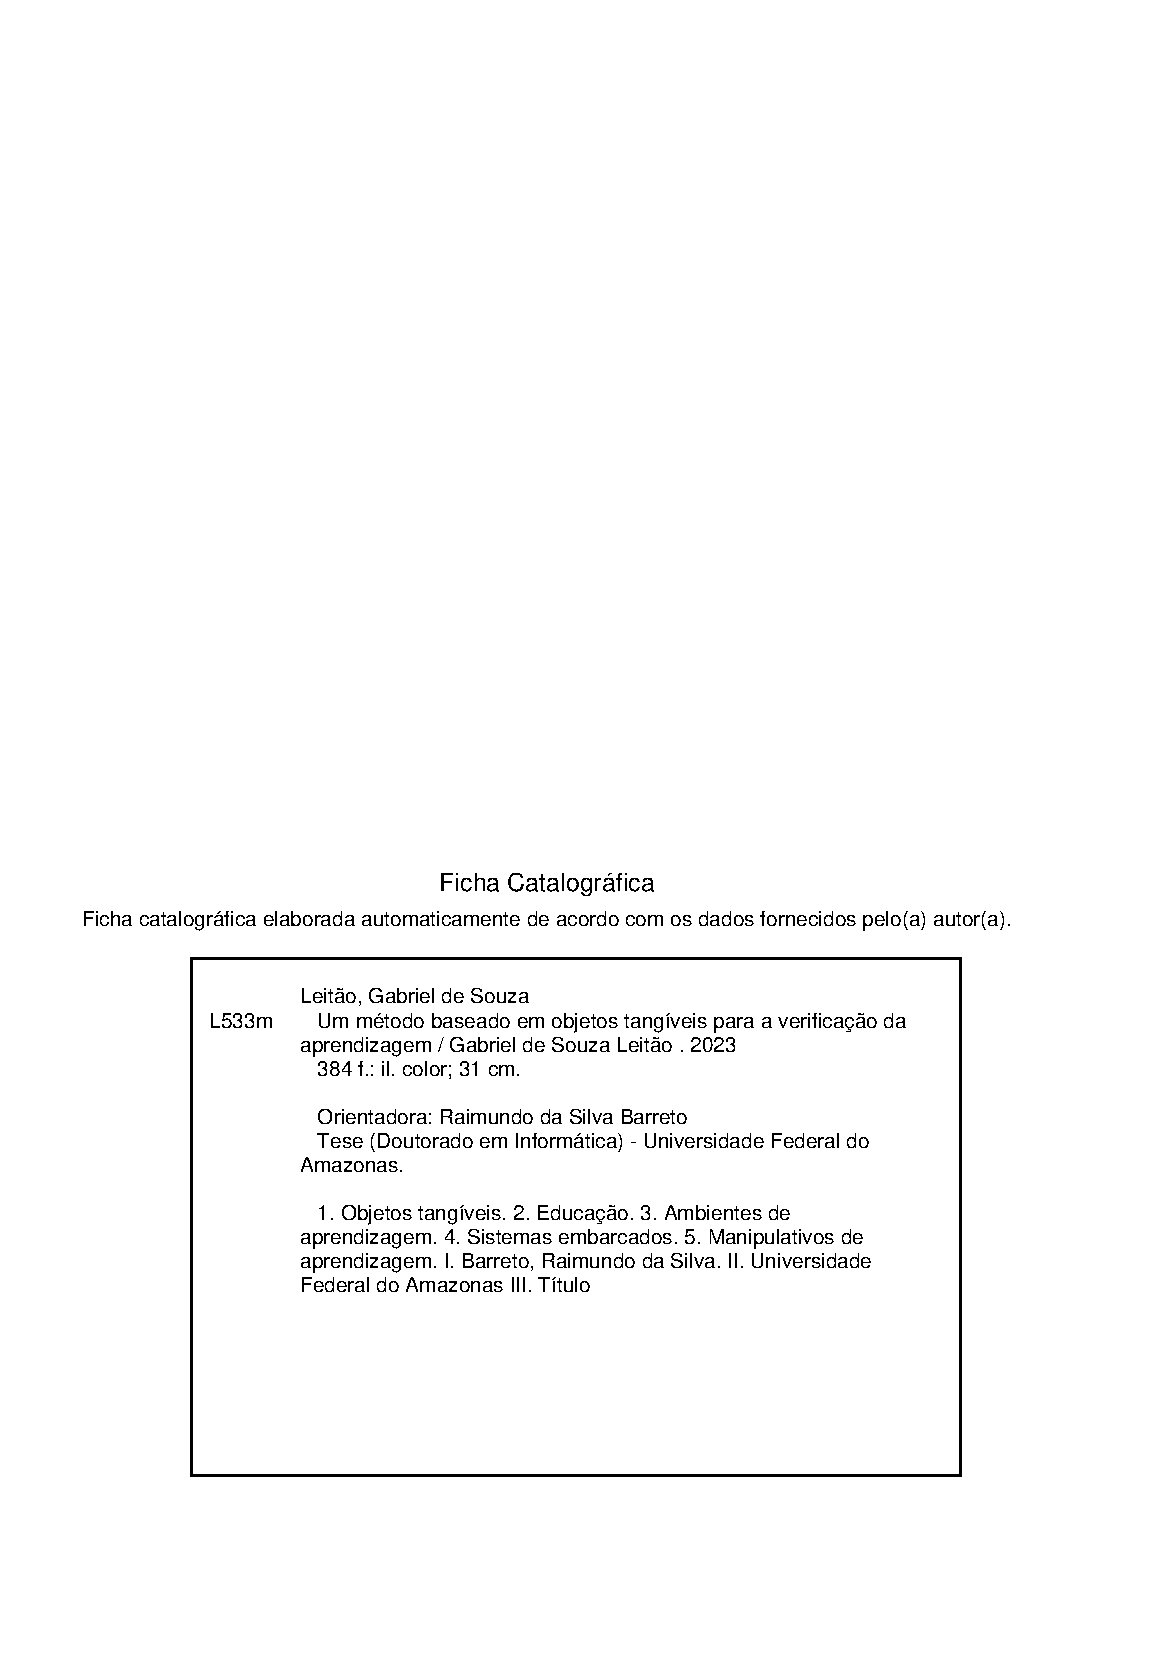
\includepdf[pages=-,offset=75 -75] {Presentation/Documentos/fichacatalografica.pdf}

%\imprimirfolhadeaprovacao
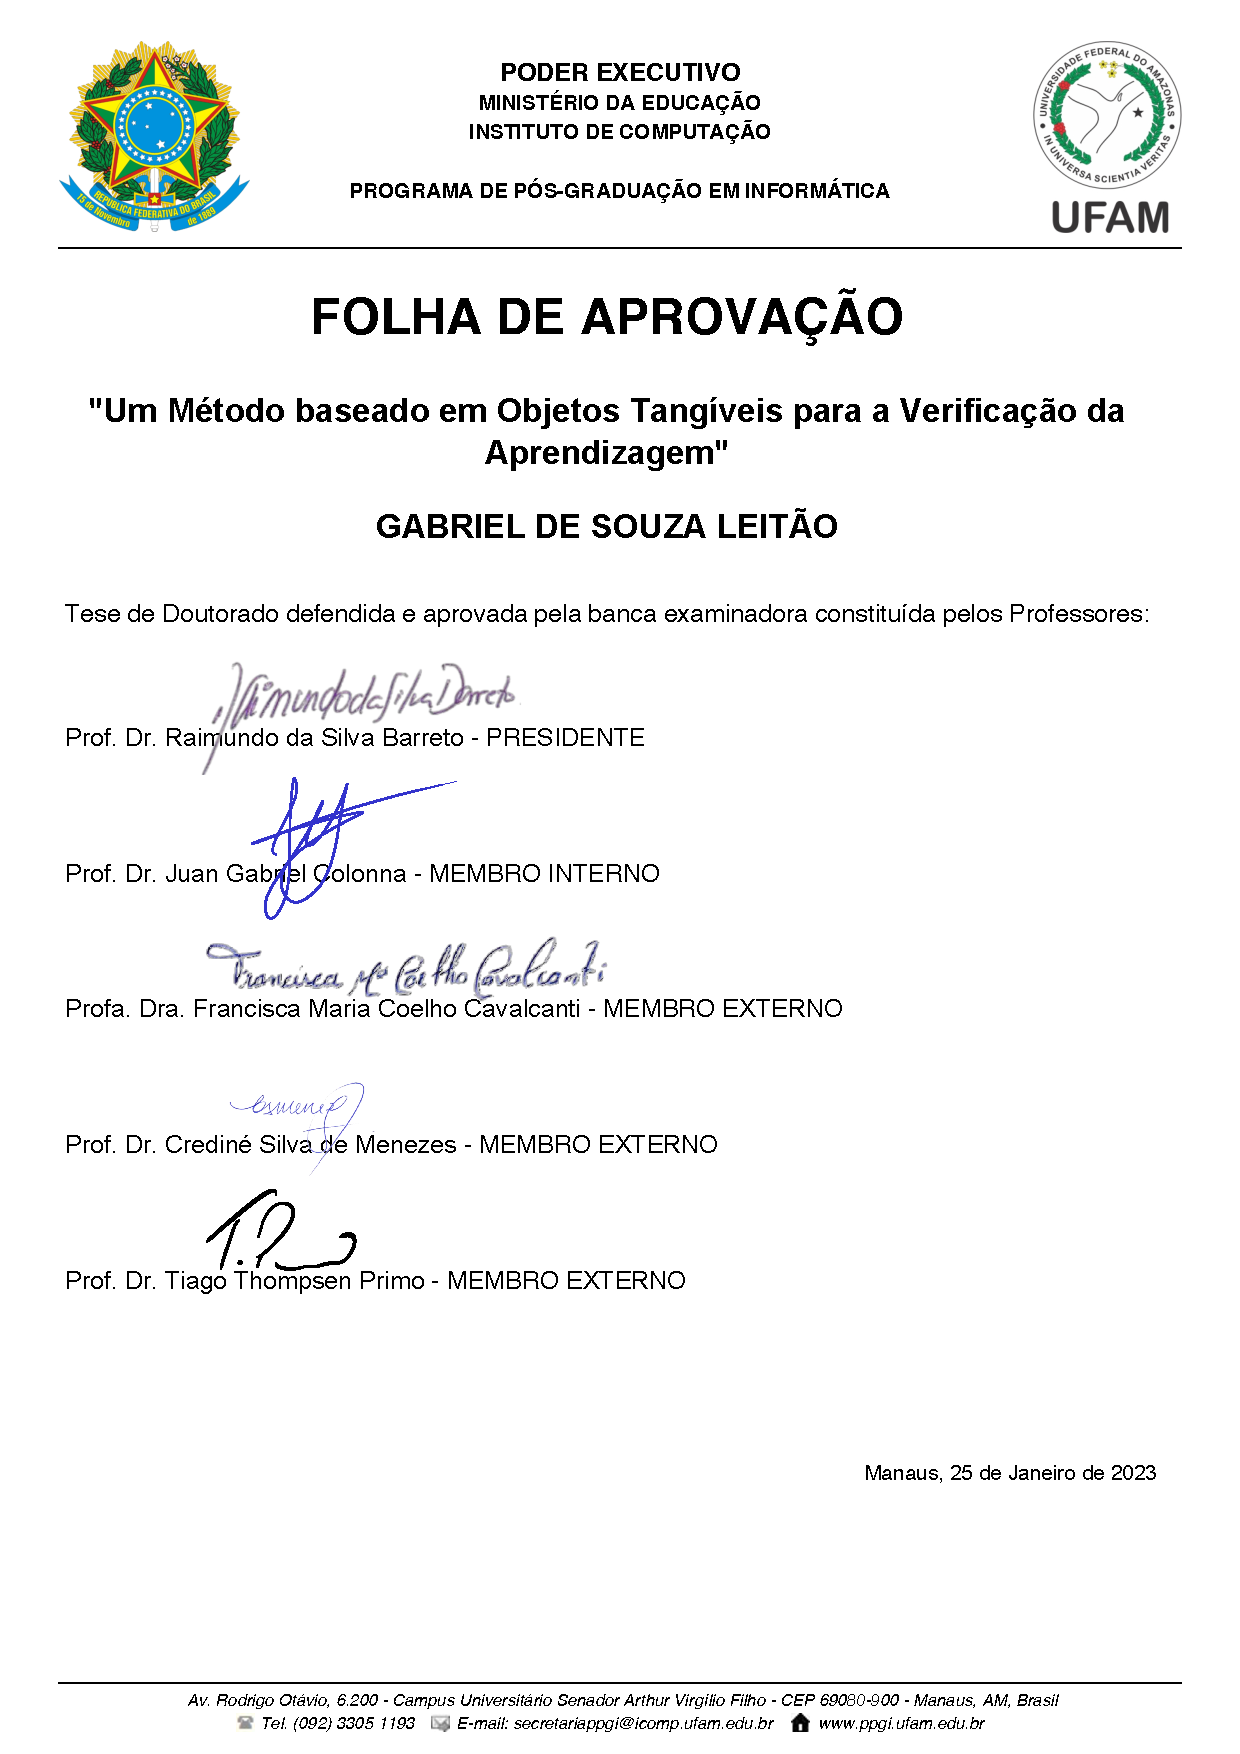
\includepdf[pages=-,offset=75 -75] {Presentation/Documentos/folhaaprovacao.pdf}




% % % % % % % % % % % % % % % % % % % % % % % % % % % % % % % % % % % % % % % 
% % -------------------- Código para personalização
%para os códigos em C
\lstset{language=C,basicstyle=\scriptsize}
% 
% 
\lstset{numbers=left, numberstyle=\tiny, stepnumber=1, numbersep=5pt}
\lstset{firstnumber=1}
\lstset{frame=single}
\lstset{showstringspaces=false}
\lstset{showspaces=false}
\lstset{showtabs=false}
\lstset{tabsize=2}
\lstset{
	language={C},
	morekeywords={assert,uchar,sizeof_FORTES}
}
% % % % % % % % % % % % % % % % % % % % % % % % % % % % % % % % % % % % % % % 





% % % % % % % % % % % % % % % % % % % % % % % % % % % % % % % % % % % % % % % % % % % % % 
% % % % % Begin Chapters

% -----------------------------------------------------------------
% => DEDICATORIA
% -----------------------------------------------------------------
\dedicatory{Esta Tese é dedicada à minha família, meu apoio em todos os momentos.}

% -----------------------------------------------------------------
% => AGRADECIMENTOS
% -----------------------------------------------------------------
\acknowledgements{
%Primeiramente, agradeço a vida e a saúde que me foram concedidas ao longo destes árduos tempos, foram muitas dificuldades, mas, todas superadas com paciência e auxílio de quem me acompanhou nessa jornada.

% Agradeço à minha família, meu esteio, sem os quais seria impossível eu ter chegado onde estou. Eu sou extremamente grato por todo o carinho, atenção e disponibilidade que vocês tem tido comigo ao longo dos anos.

%Especialmente, agradeço à minha esposa, Thais Augusto do Nascimento, pelo constante apoio e carinho, mas, principalmente, pela compreensão com as dificuldades inerentes a este processo e pelas discussões e ideias que muito contribuíram para o desenvolvimento desta pesquisa. Obrigado por estar comigo e me ajudar a abrir os olhos para as possibilidades dos diversos processos educativos.

%% Primeiramente, agradeço a Deus, sem o qual nada teria sido possível. Agradeço especialmente por tanto bem e tantas dádivas recebidas através das pessoas que me acompanharam, apoiaram e auxiliaram nesta pesquisa. Todas são sinais da presença amorosa de Deus na minha vida.

%%Primeiramente, agradeço a Deus por tanto bem e tantas dádivas recebidas através das pessoas que me apoiaram nesta pesquisa. Todas são sinais da Sua presença amorosa em minha vida. 

% Ao meu orientador e amigo, professor Raimundo da Silva Barreto, que tem acompanhado grande parte da minha odisseia acadêmica, desde os primeiros anos na graduação em Engenharia da Computação, minha temporada na Filosofia e, então, o meu retorno para continuar os estudos no Mestrado em Informática. Muito obrigado, professor, pela amizade, humanidade, orientação e, especialmente, por toda a confiança que tem depositado em mim e no meu processo.

% Às professoras Elaine Harada Teixeira de Oliveira e Francisca Cavalcante e aos professores Tiago Thompsen Primo e Juan Gabriel Colonna, muito obrigado pela solicitude em aceitar participar da minha banca de defesa e pelas excelentes contribuições seja por ocasião da qualificação, seja por outros projetos relacionados com os quais estivemos envolvidos.

% Agradeço também aos meus amigos e colegas do Grupo de Interesse em Sistemas Embarcados, do PPGI/ICOMP e dos cursos de Ciência da Computação, Engenharia de Software e Engenharia da Computação da UFAM que ajudaram imensamente na discussão e implementação deste trabalho. Faço um agradecimento especial a Anilton Carlos, Adelson Portela, Jeliel Augusto, Edson Magno, Edwin Juan, Fernando Furtado, Lucas Barreto, Timoteo Santos e Victor Augusto.

% Muito obrigado aos meus colegas de trabalho do IFAM que me apoiaram no afastamento para o doutorado, na viabilização dos experimentos ou segurando as pontas na preparação para a defesa da tese. Meu agradecimento especial a Ana Maria, Ana Paula, Eline, Fábio, Hilton, Jaidson, Lerkiane, Paulo Vitor, Valéria e Walter.

% Agradeço aos estudantes dos cursos técnicos integrado em informática e em jogos digitais do IFAM de Manacapuru que aceitaram participar e colaborar com a execução dos experimentos.

%Enfim, agradeço a todas as minhas amigas e amigos que tem me apoiado e torcido pelo meu sucesso pessoal e profissional.

%% Minha gratidão a CAPES pelo suporte financeiro para execução desta pesquisa. Parte dos resultados apresentados neste trabalho foram obtidos através do projeto de pesquisa ``Sistemas para Avaliação de Comportamento e Recomendação Inteligente em Ambientes Educacionais e de Saúde Remota'', financiado pela Samsung Eletrônica da Amazônia Ltda., no âmbito  da Lei no. 8.387 (art. 2º)/91.

}

% -----------------------------------------------------------------
% => EPIGRAFE
% -----------------------------------------------------------------
\dedicatory{"(...) a minha quest{\~a}o n{\~a}o {\'e} acabar com a escola, {\'e} mud{\'a}-la completamente, {\'e} radicalmente fazer que nas{\c{c}}a dela um novo ser t{\~a}o atual quanto a tecnologia. Eu continuo lutando no sentido de p{\^o}r a escola {\`a} altura do seu tempo. E p{\^o}r a escola {\`a} altura do seu tempo n{\~a}o {\'e} soterr{\'a}-la, mas refaz{\^e}-la."~(Paulo Freire,1996,In:``Seymour Papert e Paulo Freire: uma conversa sobre informática, ensino e aprendizagem'')}

% -----------------------------------------------------------------
% => ABSTRACT
% -----------------------------------------------------------------
% -----------------------------------------------------------------
% => ABSTRACT [DOING]
% -----------------------------------------------------------------
% 
\begin{resumo}

Atualmente, nós vivemos em uma sociedade tecnológica. Por essa razão, propor novas metodologias de ensino, que integrem recursos tecnológicos, que pressuponham o uso de inteligência artificial, internet das coisas e sistemas ciberfísicos, com a finalidade de aprimorar as experiências pedagógicas e, consequentemente, a qualidade da educação é uma demanda socialmente importante. Assim, no contexto da Educação 4.0, esta tese discorre sobre a resolução de um problema que pode ser expresso através da seguinte pergunta: \textit{é possível a construção de um ambiente de educação suportado por tecnologia, que utilize recursos computacionais físico-digitais como parte integrante do processo de ensino-aprendizagem e que, adicionalmente, proveja elementos que auxiliem na avaliação e acompanhamento dos estudantes?}
%minimize a dificuldade dos professores em inserir recursos computacionais físico-cibernéticos como parte integrante da metodologia de ensino e que, adicionalmente, proveja análises, inferências e recomendações para a melhoria do processo ensino-aprendizagem?}
A proposta desta tese consiste em apresentar uma plataforma de educação apoiada por tecnologia que integre manipulativos físico-digitais e métricas de avaliação da aprendizagem e, analisar como manipulativos físico-digitais criados através do modelo proposto podem auxiliar no processo e acompanhamento do ensino-aprendizagem.
%proveja recomendações de recursos educacionais baseadas em análise inteligente de aprendizagem visando atender às diversas demandas de aprendizagem dos estudantes. 
Desse modo, foi projetada uma plataforma composta de quatro partes: (i) Compositor: componente responsável pela geração de material didático, incluindo a inserção de objetos tangíveis de aprendizagem; (ii) Player Físico-Virtual: interface multiplataforma baseada em web responsável pela execução da parte digital da aula, incluindo possibilidades de interação com objeto tangível; (iii) Servidor: cria e gerencia a sala de aula virtual, trocando mensagens com todos os dispositivos do ambiente de aprendizagem, inclusive os diversos componentes físico-digitais dos recursos pedagógicos; e, (iv) Analíticos: componente responsável por calcular as diversas métricas de aprendizagem propostas a fim de fornecer informações e análises baseadas na interação do estudante com o material didático. 
A avaliação experimental foi feita da seguinte forma: (a) análises de um estudo exploratório das métricas de aprendizagem propostas cujo objetivo foi de verificar as análises que tais métricas poderiam prover; (b) Estudo de Caso dividido em três fases com o objetivo de: (i) analisar o impacto na aprendizagem do uso do objeto tangível construído de acordo com o modelo proposto; (ii) verificar a percepção dos estudantes com relação ao uso do objeto tangível; e, por fim, (iii) explorar a viabilidade do uso de um objeto tangível para avaliação/acompanhamento da aprendizagem no contexto da plataforma proposta. 

\novo{Após a escrita do capítulo de Resultados, complementar com o que foi achado `findings'}


%Além da proposta, como resultados, são apresentados: (a) análises de experimentos prévios cujo objetivo foi de verificar as análises que as métricas propostas poderiam prover; (b) dois mapeamentos sistemáticos da literatura, onde o primeiro abordou a recomendação de recursos educacionais baseados em computação cognitiva e o segundo abordou a criação de ambientes de aprendizagem baseados em ambientes ciber-físicos; e (c) uma proposta inicial de um estudo de caso que sirva de prova de conceito para o método apresentado.

\end{resumo}
% -----------------------------------------------------------------
% => ABSTRACT [DOING]
% -----------------------------------------------------------------
% 
\begin{abstract}
Coming soon...
%We live in a technological society, therefore we must propose new teaching methodologies that integrate modern technological resources and that suppose the use of artificial intelligence, internet of things and cyber-physical systems to improve pedagogical experiences and, consequently, the quality of education. Thus, in the context of Education 4.0, this thesis discusses the resolution of a problem that can be expressed through the following question: `\textit{is it possible to build a technology-supported education environment that minimizes the difficulty for teachers to insert physical-cyber computing resources such as essential part of learning methodology and that, in addition, provides analysis, inferences and recommendations to improvement of teaching-learning process?}' For this reason, the purpose of this thesis is to present a technology-supported education platform that enables the integration of learning objects that have at the same time, integrated physical and virtual components and which, after a classroom, provides recommendations of educational resources based on learning analytics to answer the diverse learning demands of students. Thus, a platform composed of five parts was designed: (i) Composer: component responsible for the generation of didactic material, including the insertion of physical-virtual learning objects; (ii) Physical-Virtual Player: runs the class with relative independence to the execution environment; (iii) Server: creates and manages the virtual classroom, exchanging messages with all devices in the learning environment, including the various physical and virtual components of pedagogical resources; (iv) Analytics: component responsible for calculating the learning metrics proposed in order to provide information and analysis based on student interaction with the didactic material; and (v) Intelligence: responsible for recommending educational resources and making notifications regarding student demand for study. Besides the proposal, as results, are presented: (a) analyzes of previous experiments whose objective was to verify the analyzes that the proposed metrics could provide; (b) two literature systematic mappings, where the first approached the recommendation of educational resources in cognitive computing-based and the second approached the creation of cyber-physics based learning environments; and (c) an initial proposal for a case study that will serve as proof of concept for the method presented.

\end{abstract} 



% % % % % % 
% Sumario
% % % % % % 
\pdfbookmark{\contentsname}{toc} % NEW
\tableofcontents

\listoffigures
\listoftables

\newpage
%\phantomsection \label{listalgorithmcfname}
%\addcontentsline{toc}{chapter}{\listalgorithmcfname}
%\listofalgorithms

\renewcommand{\listingscaption}{Código-fonte}
\renewcommand\listoflistingscaption{Lista de Códigos-fonte}
\listoflistings

% Empty page
\newpage
\thispagestyle{empty} 
\mbox{}




% -----------------------------------------------------------------
% => LISTA DE ABREVIACOES E ACRONIMOS
% -----------------------------------------------------------------
\input{chapters/listaAbreviacoesAcronimos.tex}

\mainmatter




% -----------------------------------------------------------------
% => INTRODUCTION - 1 [DOING]
% -----------------------------------------------------------------
% 
% -----------------------------------------------------------------
% => INTRODUCTION - 1
% -----------------------------------------------------------------
\chapter{Introdução} \label{Chap:intro}

Na sociedade atual, os artefatos tecnológicos são parte integrante da vida das pessoas, moldando seu relacionamento consigo mesmas e com o mundo~\citep{Leitao:2014}. Além disso, a possibilidade de armazenar e analisar grandes volumes de dados tem permitido que tecnologias baseadas em Inteligência Artificial (IA) sejam cada vez mais utilizadas para melhorar processos nos mais diversos setores da sociedade, facilitando tomadas de decisões e reduzindo desperdícios de recursos. Assim, em 2011, na Feira de Hannover (Alemanha) cunhou-se o termo ``Indústria 4.0'' que denomina uma Quarta Revolução Industrial, cujo objetivo é tornar os processos industriais mais inteligentes e autônomos utilizando, dentre outras coisas, Inteligência Artificial, Sistemas Ciber-Físicos (CPS) e a emergente Internet das Coisas (IoT)~\citep{MCDIC:2014, Almeida:2018}.

%Segundo \cite{bassedas:1996}, o objetivo da escola, enquanto instituição, é a educação dos alunos que, para ele, significa a transmissão e o ensino de conteúdos determinados. Num sentido amplo, esses conteúdos seriam conceitos, acontecimentos, procedimentos, atitudes, valores e normas. Desse modo, pode-se afirmar que a função principal da escola é introduzir o indivíduo na sociedade.

Para cumprir mais eficazmente o seu papel de integração e socialização da cultura e do conhecimento, a escola não teria como passar imune a essa nova revolução~\citep{Nogueira:2013, Levy:2010}. Assim, a escola precisa, não somente inserir recursos tecnológicos dentro dos processos de ensino-aprendizagem, mas, propor novas metodologias e práticas pedagógicas~\citep{Sousa:2011} que, integradas às novas tecnologias, ajudem os alunos a desenvolver as competências e habilidades necessárias a dinamicidade do novo mundo a partir da nova revolução industrial~\citep{Fuhr:2018}, isto é, ultrapassando a noção de educação como mera aquisição de conhecimento fechado e em escala industrial, proveniente das duas primeiras revoluções industriais~\citep{Intelitek:2018}.

% A sociedade atual é profundamente marcada pela tecnologia, o que implica que os artefatos tecnológicos não são tratados como simples ferramentas, mas, como parte integrante da vida das pessoas, moldando o modo como elas se relacionam consigo mesmas e com o mundo ao seu redor \citep{EspiritoSanto:2012,Leitao:2014}. Assim, para cumprir mais eficazmente a sua função social, a escola precisa integrar os recursos tecnológicos nos processos de ensino propondo novas metodologias e práticas pedagógicas \citep{Sousa:2011}.

Essa demanda de integração da tecnologia nos ambientes educacionais tem possibilitado a construção de novos cenários de aprendizagem e a utilização de ferramentas que colaborem, tanto com os processos de ensino quanto de avaliação do desempenho dos estudantes, através do reconhecimento de contextos, atividades ou comportamentos dos estudantes durante a aula e, assim, façam recomendações com o objetivo de melhorar a qualidade da educação~\citep{Cheng:2006,Dong:2007,Mathioudakis:2013}. Tal integração pode envolver aplicações dos conceitos de Internet das Coisas, Inteligência Ambiental ({\it Ambient Intelligence}), Aprendizagem Ubíqua, Ciência de Contexto ({\it context-awareness}), Sistemas Multiagente e Sistemas Ciberfísicos~\citep{Oluwagbemi:2014,Xue:2011} e tem sido chamada de \textbf{Educação 4.0}~\citep{Hussin2018}.

Além disso, especialmente relacionado aos sistemas ciberfísicos, é importante destacar que a integração de interfaces tangíveis (Seção~\ref{section:TUI}) em ambientes de aprendizagem, tornando-os ambientes tangíveis, adicionam novas perspectivas ao processo de ensino-aprendizagem, uma vez que a metodologia pedagógica pode ser expandida para além dos objetos de aprendizagem tradicionais (baseados apenas em interação virtual), passando a incluir também manipulativos físicos dentro de um horizonte computacional.

% Entretanto, apenas criar ou utilizar recursos educacionais tecnológicos não garante a eficácia e nem a melhoria da qualidade da educação, pois, o aproveitamento de uma aula está relacionado ao engajamento do aluno no processo de ensino-aprendizagem. Assim, o uso de tecnologias em sala de aula também poderia permitir inferências como engajamento, nível de entendimento e dificuldades dos estudantes ao longo de um processo educativo~\citep{Gligoric:2015,Leitao:2015}. Tais inferências podem auxiliar o professor na criação ou modificação de conteúdos educacionais mais adequados ao perfil e necessidades de uma turma ou de um estudante.

% -----------------------------------------------------------------
% => CONTEXTO
% -----------------------------------------------------------------
\section{Contexto}
\label{section:contexto}

Segundo \cite{bassedas:1996}, o objetivo da escola, enquanto instituição, é a educação dos alunos que, para ele, significa a transmissão e o ensino de conteúdos determinados. Num sentido amplo, esses conteúdos seriam conceitos, acontecimentos, procedimentos, atitudes, valores e normas. Desse modo, pode-se afirmar que a função principal da escola é introduzir o indivíduo na sociedade.

Além disso, para o sociólogo da educação Pierre Bourdieu, o sucesso  escolar do estudante depende de levar em consideração a bagagem que ele traz consigo~\citep{Nogueira:2013}. Desse modo, o uso de um determinado capital cultural (por exemplo, o uso de dispositivos móveis e da internet) previamente pertencente ao estudante facilitaria o processo de ensino-aprendizagem dos códigos e conteúdos transmitidos pela escola formal. Além disso, para \cite{bassedas:1996}, tal processo possui três elementos: o estudante, os conteúdos de aprendizagem e o professor.

% Assim, para melhoria e maior eficiência do processo de ensino-aprendizagem, é preciso levar em consideração a grande familiaridade que as crianças e jovens tem com as novas tecnologias e inseri-las definitivamente na educação. Por isso, este trabalho está situado no contexto do desenvolvimento de ambientes de sala de aula inteligente com enfoque na utilização de objetos de aprendizagem físico-virtuais (com interfaces concretas e virtuais integradas) como ferramenta de apoio aos processos de ensino e de avaliação da aprendizagem.

%anterior Assim, tendo em vista as infinitas possibilidades que emergem da Educação 4.0, este trabalho está situado no contexto do desenvolvimento de ambientes físico-virtuais de aprendizagem com enfoque na utilização de ferramentas de apoio às atividades do professor e do estudante. No lado do professor, o suporte acontece na geração, uso e avaliação de materiais didáticos e desempenho dos estudantes. No lado do estudante, a novidade está na inserção de ferramentas e objetos de aprendizagem físico-virtuais que se adaptem às suas necessidades e ao ambiente, possibilitando que o mesmo possa construir experiências que levem à construção de conhecimento.

%atual
Assim, tendo em vista as infinitas possibilidades que emergem da Educação 4.0, este trabalho está situado no contexto do desenvolvimento de ambientes tangíveis de aprendizagem com enfoque na utilização de ferramentas de apoio às atividades do professor e do estudante. No lado do professor, a novidade está na geração e no uso de materiais didáticos diferenciados que possibilitem inclusive uma avaliação da aprendizagem dos estudantes. No lado do estudante, a novidade está na inserção de ferramentas e objetos tangíveis de aprendizagem que sejam mais interessantes do que o ensino tradicional, possibilitando que o mesmo possa executar atividades que levem à construção de conhecimento.

%anterior Como ponto de partida, tem sido aprimorada uma plataforma implementada ao longo do projeto de mestrado do proponente, a qual é composta de quatro partes: (i) Compositor, que é uma ferramenta para geração de material didático a partir de objetos de aprendizagem inseridos pelo professor ou provenientes de um repositório; (ii) Player, que propõe uma interface multiplataforma responsável pela execução da aula em dispositivo portátil, incluindo possibilidades de interação físico-virtual; (iii) Servidor, que é responsável pela criação, gerenciamento da sala de aula e adaptação do conteúdo educacional a partir das análises feitas dos dados obtidos da interação do estudante com o conteúdo educacional; e (iv) Analytics, que é responsável pela análise de dados para tomadas de decisão e geração de gráficos que auxiliem o professor na percepção do impacto de determinada atividade educacional na turma e futuras tomadas de decisões metodológicas. Tais ferramentas serão melhor apresentadas ao longo desta proposta, onde também serão introduzidas as futuras modificações para implementação do novo sistema.

Como ponto de partida, foi aprimorada uma plataforma inicialmente proposta na dissertação de mestrado de \cite{leitao:2017}, a qual é composta de quatro partes: (i) Compositor, que é uma ferramenta para geração de material didático a partir de objetos de aprendizagem inseridos pelo professor ou provenientes de um repositório; (ii) Player, que propõe uma interface multiplataforma responsável pela execução da aula em dispositivo portátil, incluindo possibilidades de interação tangível; (iii) Servidor, que é responsável pela criação, gerenciamento da sala de aula, exibição dos recursos educacionais, além da comunicação entre as partes do objeto tangível de aprendizagem; e (iv) Analíticos, que é responsável pelo cálculo das métricas de avaliação da aprendizagem e pela geração de gráficos que auxiliem o professor na percepção do impacto de determinada atividade educacional na turma e futuras tomadas de decisões metodológicas. Tais ferramentas serão melhor apresentadas ao longo desta proposta, onde também serão introduzidas as futuras modificações para implementação do novo sistema.

% -----------------------------------------------------------------
% => Definição do Problema
% -----------------------------------------------------------------
\section{Definição do Problema}
\label{section:defProblem}

Segundo o filósofo francês \cite{Levy:2010}, a partir dos anos 80, com a invenção e popularização do computador pessoal, a informática foi perdendo seu {\it status} de técnica aplicada somente ao setor industrial, para fundir-se à cultura, tornando-se cada vez mais integrada às relações sociais, trabalhistas e organizacionais, criando um ambiente virtual (cibernético) baseado em bits, memórias, grande capacidade de processamento e transmissão de dados.

Assim, num mundo cada vez mais digitalizado, \cite{Kenski:2007} afirma que o papel social das tecnologias da informação nas relações humanas permite novas e diferentes possibilidades para a educação à medida que transformam ou mesmo transcendem o espaço físico em que ela ocorre e à medida que possibilitam novas relações com os conhecimentos e com o outro, onde todos se tornam educadores e aprendizes.

%anterior já comentado
%Essa novas relações com o mundo, proporcionadas pela tecnologia, tem propiciado uma revolução no ensino e promovido o desenvolvimento de diversas modalidades de ensino à distância. Em contraposição, o ensino presencial tradicional tem enfrentado muitas dificuldades em modificar suas ferramentas e atualizar seus modelos. Dentre essas dificuldades, \cite{EspiritoSanto:2012} afirma que o maior problema está relacionado à falta de experiência ou conhecimento dos docentes no manuseio de computadores, o que implica em deficiência na inserção espontânea de tais elementos como parte da metodologia de ensino-aprendizagem, tornando as aulas desinteressantes e monótonas.

%reescrito e readicionado
Essa novas relações com o mundo, proporcionadas pela tecnologia, tem propiciado uma revolução no ensino e promovido o desenvolvimento de diversas modalidades de ensino à distância e, mais recentemente, com a pandemia de COVID-19, a utilização do ensino remoto emergencial evidenciou ainda mais a necessidade de uma maior integração entre a educação presencial e os novos recursos tecnológicos existentes, de modo a minimizar as dificuldades encontradas quando da necessidade de distanciamento físico entre os participantes do processo educacional.
%Diante disso, é importante salientar que o ensino presencial tradicional (e de forma análoga o ensino remoto) tem enfrentado muitas dificuldades em modificar suas ferramentas e atualizar seus modelos, dentre essas dificuldades, \cite{EspiritoSanto:2012} afirma que o maior problema está relacionado à falta de experiência ou conhecimento dos docentes no manuseio de computadores, o que implica em deficiência na inserção espontânea de tais elementos como parte da metodologia de ensino-aprendizagem, tornando as aulas desinteressantes e monótonas.

O problema considerado nesta Tese pode ser expresso através da seguinte pergunta: 
%é possível a construção de um ambiente de educação suportada por tecnologia, que minimize a dificuldade dos professores em inserir recursos computacionais como parte integrante da metodologia de ensino e que, adicionalmente, proveja análises, inferências e recomendações para a melhoria do processo ensino-aprendizagem e atue como um assistente virtual de aprendizagem baseado em ciber-física?
é possível a construção de um ambiente de educação suportado por tecnologia que utilize recursos computacionais tangíveis como parte integrante do processo de ensino-aprendizagem e que, adicionalmente, proveja elementos que auxiliem na avaliação e acompanhamento dos estudantes?

O problema em questão, da construção de ecossistemas tangíveis de aprendizagem, traz consigo uma série de desafios inerentes, tanto ao componente físico quanto ao componente digital, tais como os apresentados por \cite{Leitao:2019}: (i) como \textit{registrar as interações} entre os estudantes e o ambiente físico-digital, e como usar tais informações para  \textit{avaliar a experiência de aprendizado} e das condições do ambiente de ensino; (ii) como identificar as eventuais  \textit{ações corretivas} a serem tomadas; (iii) quais \textit{recomendações} podem ser feitas para melhorar a qualidade da aprendizagem; e (iv) como \textit{definir o progresso}, ou falta dele.
%
Para tanto, dentro do contexto de ambientes tangíveis, há ainda a necessidade de métodos, técnicas e ferramentas que consigam medir o progresso de cada aluno individualmente e em grupo, e como recomendar experimentos tangíveis para que um aluno venha a melhorar o seu desempenho acadêmico.

Além disso, algumas dificuldades potenciais inerentes a esses desafios foram identificadas e estão descritas a seguir: (i) na base de dados do CBIE há apenas três artigos que tratam especificamente desse tema, onde apenas um deles propõe uma plataforma básica para implementação de ambientes físico-virtuais na educação~\citep{Santos:2014}; (ii) há um problema de se fazer recomendações e avaliações de objetos tangíveis uma vez que não há um repositório dos mesmos; (iii) há um problema para a criação e descrição de objetos tangíveis de aprendizagem porque não há um padrão de metadados e/ou ontologias que tratem desses objetos de forma adequada; e (iv) há uma problema de sistematização da execução desses objetos, visto que os objetos criados não estão integrados a nenhuma plataforma ou a quaisquer ambientes de aprendizagem.

A resolução desses problemas demanda um bom esforço da comunidade científica, mas, pode abrir caminho não apenas para a obtenção de dados empíricos de interação dos estudantes com o material didático do tipo manipulativo físico, mas, a análise desses dados proverá um conhecimento dos processos de aprendizagem dos estudantes que possibilitará: (a) adaptação dos conteúdos das aulas, a partir das necessidades da turma e durante a aula; (b) geração de recomendações ao professor relacionadas a atividades pedagógicas que mais ajudem a sanar deficiências de aprendizagem; (c) extensão do ambiente de aprendizagem para todo e qualquer lugar, de forma que o estudante possa construir e aprofundar conhecimentos a partir da interação com o mundo físico.


% -----------------------------------------------------------------
% => Motivação
% -----------------------------------------------------------------
\section{Motivação}
\label{section:motivation}

% % Aqui é o ?POR QUÊ?, ou seja, visa responder o porquê é importante resolver tal problemas, quais os benefícios, melhorias, etc.

Na Seção~\ref{section:defProblem} (Definição do Problema) foi comentado sobre como o advento e a popularização da informática provocaram uma revolução social e modificaram profundamente o modo como as pessoas se relacionam consigo mesmas e com o mundo. Não obstante, a computação  continua evoluindo, inovando e tornando-se cada vez mais ubíqua.

Essa ubiquidade da computação está atrelada ao emergente conceito de computação pervasiva que, segundo~\cite{Satyanarayanan:2001}, é caracterizada não apenas pela invisibilidade dos recursos computacionais por parte dos usuários, mas, também pelo aprofundamento da noção de espaços inteligentes, que se adaptam aos mais diversos contextos.

Além disso, de acordo com~\cite{Caron:2018}, a nova educação, que surge da revolução da Educação 4.0, precisa ajudar os alunos a desenvolver habilidades como: (i) comunicação e colaboração; (ii) iniciativa e empreendedorismo; (ii) pensamento crítico e analítico; (iv) curiosidade e imaginação; e, (v) domínio das tecnologias. Para tanto, tem-se intuído que o uso de metodologias ativas é essencial, isto é, as estratégias pedagógicas precisam levar em consideração o protagonismo do aluno no processo de aprendizagem.

\cite{Andrade:2018} elenca cinco abordagens que implementam metodologias ativas no contexto educacional: (i) Ensino Híbrido, cuja base é a integração entre o ensino online e offline; (ii) Aprendizagem Baseada em Projetos, cujo trabalho de investigação é responder uma pergunta ou desafio complexo; (iii) Sala de Aula Invertida, onde, primeiramente, os alunos estudam o conteúdo em casa e, então, na escola, todos compartilham e esclarecem dúvidas e aprendizados mediados pelo professor; (iv) STEAM, que é uma forma de aprendizagem interdisciplinar com enfoque prático nas áreas de Ciências, Tecnologia, Engenharia, Arte e Matemática; e, por fim, (v) Cultura Maker, que visa ser uma abordagem de aprendizagem criativa e prática, baseada no princípio DIY (\textit{Do It Yourself}), que tem usado plataformas de prototipagem eletrônica como Arduíno e Microbit no contexto educacional. Entretanto, é importante salientar que uso de uma ou outra abordagem depende principalmente dos objetivos pedagógicos e dos objetos de aprendizagem utilizados de modo que, por princípio, a plataforma proposta neste trabalho deve possibilitar a escolha da estratégia mais adequada a cada caso.

Dessa forma, a inserção e utilização de recursos computacionais no processo de ensino-aprendizagem presencial serve a uma dupla finalidade, a saber:

\begin{enumerate}
	\item \textbf{Revisão e adaptação do método de ensino:} Mais do que mera inserção de novas tecnologias, o uso de ferramentas computacionais no ambiente de sala de aula motiva uma verdadeira revisão dos métodos de ensino. Tal reformulação permite tornar o processo de aprendizagem mais atraente, especialmente por privilegiar e oportunizar uma dimensão de interatividade com o conteúdo educacional, seja através de jogos, de laboratórios virtuais ou de desafios que instiguem a capacidade de resolução de problemas~\citep{Sousa:2011,Chang:2014,Hwang:2009,Dekdouk:2012}, seja através de dicas, curiosidades ou conteúdos sugeridos a partir das interações físicas do estudante captadas pelo sistema~\citep{Santos:2014}.
	
	\item \textbf{Maior conhecimento formal do perfil dos estudantes:} Com o apoio de tecnologias capazes de obter dados de interação dos estudantes ao longo do processo de aprendizagem, torna-se possível a geração de gráficos e análises que ofereçam suporte ao professor na avaliação e nas tomadas de decisão que envolvam, por exemplo, a adição de atividades pedagógicas que reforcem a aprendizagem de um conteúdo ou competência, além de estratégias pedagógicas potencialmente mais eficientes. Assim, os dados obtidos a partir das aulas e processos avaliativos podem permitir melhores inferências relacionadas ao perfil de aprendizagem e às dificuldades de uma turma ou estudante e, assim, recomendações de atividades ou estratégias mais adequadas e adaptadas às suas necessidades e demandas.
\end{enumerate}

Não obstante os riscos e dilemas éticos da inserção de novas tecnologias no processo de ensino-aprendizagem, tais como o monitoramento constante das atividades dos atores envolvidos nos processos, a possibilidade de um maior controle do indivíduo, o uso dos saberes e recursos prévios dos estudantes e, ainda, a inserção de sistemas tangíveis, que mesclam as interações físicas com os conteúdos curriculares, pode motivá-los, diminuindo assim as barreiras para construção e, posterior retenção de conhecimento~\citep{Nogueira:2013, Sousa:2011}. 

% Apesar das vantagens já apresentadas, não podemos nos esquivar de que os dados obtidos com a inserção das novas tecnologias no processo de ensino-aprendizagem trazem consigo a possibilidade de uma discussão ética, devido a ocorrência de um necessário monitoramento das atividades dos atores envolvidos nos processos, o que abriria margem para um maior controle do indivíduo, risco da diminuição da liberdade ou, ainda, certa desmaterialização das experiências humanas~\citep{Demo:2010,Levy:2010}. Esta última, advinda da virtualização dos ambientes de aquisição do conhecimento.

% %%%
% Não obstante os riscos e dilemas da inserção de novas tecnologias no processo de ensino-aprendizagem, o uso dos saberes e recursos prévios que os estudantes trazem consigo pode motivá-los, diminuindo assim as barreiras para aquisição e retenção de conhecimento~\citep{Nogueira:2013,Sousa:2011}, bem como oferecer um melhor suporte ao professor ao prover um conjunto de ferramentas que o auxiliem na construção, execução, manutenção e revisão dos planos e estratégias de ensino.


% -----------------------------------------------------------------
% => Objetivos -> Geral
% -----------------------------------------------------------------
\section{Objetivos}
\label{section:goals}

%antigo
%O objetivo principal deste trabalho é \textit{propor uma plataforma de educação apoiada por tecnologia que integre objetos físico-virtuais de aprendizagem e que, após uma aula presencial, utilize análise inteligente de aprendizagem para recomendar conteúdos educacionais que proporcionem experiências de construção de conhecimento e melhoria do aprendizado do estudante.}

% plataforma brasil
%O objetivo principal deste trabalho é analisar como Objetos Físico-Virtuais de Aprendizagem(OFVA) criados através do modelo proposto podem auxiliar no processo e no acompanhamento do ensino-aprendizagem. Tal objetivo pode ser traduzido através das seguintes questões fundamentais: (1) Qual o impacto do uso de um OFVA na aprendizagem? (2) Qual a diferença entre uso de OFVA e o ensino tradicional?

%O objetivo principal deste trabalho é propor uma plataforma de educação apoiada por tecnologia que integre Objetos Físico-Virtuais de Aprendizagem (OFVA) e que  possibilite o acompanhamento e a verificação da aprendizagem baseados em métricas.

Propor uma plataforma de educação apoiada por tecnologia que integre manipulativos tangíveis e métricas de avaliação da aprendizagem e, analisar como manipulativos tangíveis criados através do modelo proposto podem auxiliar no processo e acompanhamento do ensino-aprendizagem.

%O objetivo principal deste trabalho é \textit{propor} um modelo de criação de Objetos Físico-Virtuais de Aprendizagem (OFVA) que possibilite acompanhamento e verificação da aprendizagem e \textit{analisar} como OFVAs criados através deste modelo podem auxiliar no processo e no acompanhamento do ensino-aprendizagem. Tal objetivo pode ser traduzido através das seguintes questões fundamentais: (1) Qual o impacto do uso de um OFVA na aprendizagem? (2) Qual a diferença entre uso de OFVA e o ensino tradicional?


% Objetivos -> Objetivos Específicos

Os objetivos específicos são:

%\begin{enumerate}
%    \item Apoiar o docente na preparação, durante e após uma aula focadas em um ambiente de ensino-aprendizagem apoiado por tecnologia;
%    \item Propor uma abordagem para integração de objetos de aprendizagem físico-virtuais a plataforma já existente no grupo de pesquisa.
% 	\item Aplicar métricas que permitam acompanhar e avaliar com maior precisão o desempenho de uma turma na interação com o material didático, indicando os tópicos e procedimentos em que os estudantes tiveram mais dificuldades.
%    % \item Propor uma metodologia pedagógica adaptativa, tanto durante quanto após as aulas;
%    \item Gerar recomendações de atividades pedagógicas, baseado em análise de aprendizagem e em objetos de aprendizagem, que complementem ou reforcem o que foi estudado em sala de aula.
%    \item Avaliar a experiência do usuário a partir dos pontos de vista do docente e do discente.
%\end{enumerate}

\begin{enumerate}
    \item Propor um método de composição e execução de aulas que integre objetos tangíveis de aprendizagem;
    \item Propor uma forma de registro das interações entre os estudantes e o ambiente tangível, gerando métricas de aprendizagem que avaliem a experiência de aprendizado;
%    \item Propor uma forma de registro das interações entre os estudantes e o ambiente físico-virtual, gerando métricas de aprendizagem que avaliem a experiência de aprendizado e das condições do ambiente de ensino;
%    \item Gerar recomendações de atividades pedagógicas que integrem objetos de aprendizagem físico-virtuais que complementem ou reforcem os conteúdos estudados;
%    \item Avaliar a utilidade da interação entre os componentes físicos e virtuais para o ensino-aprendizagem
	\item Verificar se um objeto tangível de aprendizagem criado usando o modelo de processos proposto colabora positivamente para a aprendizagem;
	\item Comparar um objeto tangível de aprendizagem criado usando o modelo de processos proposto e o modelo tradicional de ensino;
	\item Identificar a aceitação dos estudantes com relação a utilização de objeto tangível de aprendizagem no processo de ensino-aprendizagem;
	\item Identificar como um objeto tangível de aprendizagem criado usando o modelo de processos proposto pode ser utilizado na avaliação/acompanhamento da aprendizagem dos estudantes.
\end{enumerate}

% %%É necessário medir:
%  %Expectativas dos professores com relação a inserção de tecnologia em salas de aula
%  %Se as expectativas são cumpridas após a utilização do sistema proposto

%  %Expectativas dos alunos com o uso de tecnologia em sala de aula
%  %Se as expectativas foram atendidas


\section{Método da Pesquisa}\label{sec:metodologia}

Os procedimentos metodológicos a serem adotados neste trabalho são baseados no paradigma construcionista, proposto por Papert e, embora sua proposta inicial utilize uma linguagem de programação chamada \textit{Logo} para mediar o processo de aprendizagem, essa abordagem pode ser extrapolada. Assim, é possível transferir as atividades propostas no Construcionismo para fora do contexto de programação~\citep{Almeida:2000}, de modo que a execução metodológica do paradigma consiste em um ciclo de quatro atividades principais (Veja Figura~\ref{fig:metodologia}), tais como apresentadas por~\cite{Valente:1993}:

%\subsection{A Abordagem Construcionista}\label{subsec:construcionismo}

%No Construcionismo, o estudante assume o papel de principal sujeito do processo educacional (aprendizagem ativa) de modo que o computador seria uma ferramenta para construção do conhecimento e do seu próprio desenvolvimento~\citep{Valente:1993}. Esse pressuposto, o diferencia de outra abordagem conhecida como Instrucionista, em que o computador e os \textit{softwares} são vistos como máquina de ensinar e são utilizados apenas ou como objeto de estudo (um componente curricular a mais) ou como meio de instrução, isto é, de simples transmissão de um conteúdo, sem preocupação de levar o estudante a um conhecimento crítico, mas, simplesmente reproduzir um conteúdo pré-estabelecido~\citep{Almeida:2000,Valente:1993}.

%Em contraposição ao Instrucionismo, que tem o foco no uso de \textit{softwares} tutoriais, Papert leva a um outro patamar as teorias construtivistas, especialmente as de Piaget. A partir da noção piagetiana de que a criança constrói novos conceitos a partir da interação com objetos do contexto em que ela vive, Papert propõe uma abordagem onde o educando, literalmente, ao construir um objeto do seu próprio interesse através do computador, constrói também seu próprio conhecimento~\citep{Valente:1993}.


\begin{enumerate}
	\item \textbf{Descrição:} descrição das ideias para solução de um problema;
	\item \textbf{Execução:} executar as ações descritas com vistas a resolver tal problema;
	\item \textbf{Reflexão:} refletir sobre o produto da ação, sobre os conceitos empregados, sobre os erros ou falhas durante o processo;
	\item \textbf{Depuração:} quando o resultado não corresponde ao que foi idealizado, então, é necessário revisar e modificar a descrição para novamente executar e refletir sobre a resolução do problema.
\end{enumerate}  

%antigo Para o Construcionismo, não pode haver a mera inserção de tecnologia nos processos de ensino-aprendizagem e uma melhor transmissão de conteúdos pré-estabelecidos não é o objetivo da informática na educação, mas, as novas tecnologias devem realizar uma transformação no modo como a educação acontece, deve-se passar a um processo em que os recursos computacionais são utilizados como ferramentas que proporcionam ao estudante meios de avançar na busca pelo conhecimento~\citep{Almeida:2000}.

%Para o Construcionismo, a mera inserção de tecnologia nos processos de ensino-aprendizagem e, assim, uma melhor transmissão de conteúdos pré-estabelecidos não é o objetivo da informática na educação, mas, as novas tecnologias devem realizar uma transformação no modo como a educação acontece, devendo-se passar a um processo em que os recursos computacionais são utilizados como ferramentas que proporcionam ao estudante meios de avançar na busca pelo conhecimento~\citep{Almeida:2000}.

%É importante salientar que, para uma real transformação da educação mediada pelo uso de computadores, é necessário haver mudança no sistema educacional, em especial, no processo de formação dos professores, visto que, são eles os principais mediadores dos processos de aprendizagem. Essa mudança deve acontecer, especialmente, no modo como a aula é preparada, conduzida e o desempenho do aluno é analisado e, o primeiro passo rumo a essa mudança é entender que a educação não é simples transferência de conhecimento, mas, um verdadeiro processo de construção do conhecimento pelo aluno, onde o computador é um catalisador e o professor um necessário mediador~\citep{Valente:1993}.


%AVISO
%------ TERMINAR DE ESCREVER ----%
%  OBS: O trabalho atual ainda está dentro da linha instrucionista, mas, com evolução, por exemplo, o uso de tecnologias de interação físico-virtal pode abrir espaço pra uma abordagem mais de construção do conhecimento do que mera aquisição e replicação.


%Na fase de \textbf{Descrição}, a Revisão \textit{Ad-hoc} foi feita como meio de buscar publicações que sirvam de artigos de controle para os Mapeamentos Sistemáticos. Além disso, foram cursadas disciplinas do Programa de Pós-graduação em Informática que pudessem ajudar na construção deste projeto de Doutorado, dentre elas, Tópicos Especiais em Inteligência Artificial cujo enfoque dado foi no uso de Computação Cognitiva e Projeto e Análise de Algoritmos, onde foram analisados algoritmos que implementam técnicas de fatoração de matrizes para sistemas de recomendação.

Na fase de \textbf{Descrição}, a Revisão da Literatura foi feita como meio de buscar publicações que sirvam de referência para a construção da tese. Além disso, foram cursadas disciplinas do Programa de Pós-graduação em Informática que pudessem ajudar na construção deste projeto de Doutorado, dentre elas, Tópicos Especiais em Inteligência Artificial cujo enfoque dado foi no uso de Computação Cognitiva e Projeto e Análise de Algoritmos, onde foram analisados algoritmos que implementam técnicas de fatoração de matrizes para sistemas de recomendação, tais conteúdos estavam previstos em uma proposta inicial de tese que foi revisada e modificada.

\begin{figure}[ht]
	\centering
	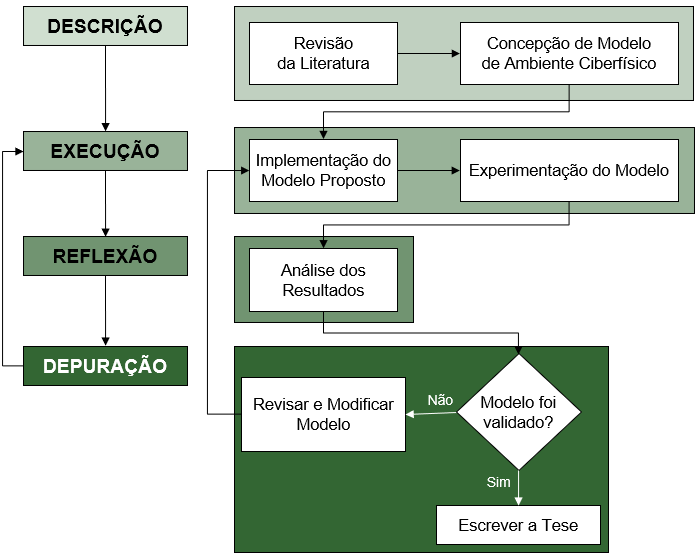
\includegraphics[width=0.8\linewidth]{imgs/METODOLOGIA_v2.png}
	\caption{Metodologia da pesquisa baseada no construcionismo de Papert}
	\label{fig:metodologia}
\end{figure}

%Com relação aos mapeamentos sistemáticos, foram planejados dois mapeamentos relativos a: (1) Recomendação de Recursos Pedagógicos utilizando sistemas computacionais cognitivos; (2) Implementação de ambientes de aprendizagem utilizando sistemas ciber-físicos. Tais mapeamentos seguem o método proposto por~\cite{kitchenham:2004} que consiste em três etapas~\citep{mafra:2006}: Planejamento do Mapeamento, Condução do Mapeamento, Análise e Publicação dos Resultados.

Ainda nessa fase, foi descrita a concepção da arquitetura e modelos do sistema proposto, tendo como base o ambiente de educação digital proposto no mestrado do proponente~\citep{leitao:2017}. Tal arquitetura foi expandida de modo a adicionar novas funcionalidades nos módulos existentes, tal como apresentado no Capítulo~\ref{Chap:prosedMethod}.

A fase de \textbf{Execução} é a fase de implementação e execução das ações descritas no Modelo com vistas a resolver o problema, além de realizar experimentos e observações para obtenção de resultados mensuráveis. Na fase de \textbf{Reflexão}, os resultados obtidos e os conceitos empregados são analisados e avaliados. Haverá também reflexão sobre os acertos, erros ou falhas ao longo do processo. A fase de \textbf{Depuração} visa revisar e, caso necessário, modificar a descrição e a implementação do Modelo fazendo ajustes para que o mesmo alcance os objetivos propostos. Assim, caso necessário, são novamente realizados as fases de ``Execução'' e ``Reflexão''.

\section{Abordagem Proposta}

Tendo em vista os desafios emanados da urgente necessidade de adaptação dos processos educacionais à nova realidade da Educação 4.0 de modo a incluir elementos de inteligência artificial, ciência de dados, internet das coisas e sistemas ciberfísicos no contexto educacional, com vistas a aprimorar as experiências de ensino-aprendizagem, tais como: a criação de ambientes de aprendizagem que incorporem elementos que tenham componentes que sejam físicos e digitais  e atuem de forma integrada; a coleta de dados de interação dos estudantes em ambos os componentes (físico e digital) de um objeto tangível; avaliação da aprendizagem através das experiências pedagógicas proporcionadas por objetos tangíveis de aprendizagem; e, a recomendação de objetos tangíveis de aprendizagem bem como a criação de padrões de metadados e de um repositório que permitam o reuso destes objetos.

%antigo Esta tese apresenta uma abordagem que expande o trabalho de mestrado de \cite{leitao:2017}, onde são propostas uma arquitetura e um conjunto de ferramentas que permitam a criação de uma aula com utilização de objetos físico-virtuais de aprendizagem, inclusive no processo de avaliação da aprendizagem. Assim, o método proposto nesta tese consiste de 5 componentes, sendo: (i) compositor: ferramenta para autoria de objetos físico-virtuais de aprendizagem que implementa uma proposta de modelo para estes objetos; (ii) servidor: \textit{middleware} para trocas de mensagens entre os componentes físicos e virtuais, além de recepção e consolidação dos dados coletados de interação dos estudantes com o material didático; (iii) player físico-virtual: interface de usuário para manipulação física ou virtual dos objetos de aprendizagem, sendo também responsável pela coleta dos dados de interação e seu envio ao servidor; (iv) analytics: módulo que implementa as métricas de avaliação da aprendizagem propostas nesta tese com o objetivo de gerar análises sobre as demandas dos estudantes; e, (v) inteligência: módulo baseado em agentes que recomendam objetos de aprendizagem ou notificam acerca das prioridades de tópicos ou disciplinas a ser estudados pelos alunos.

Esta tese apresenta uma abordagem
% que expande o trabalho de mestrado de \cite{leitao:2017},
onde são propostas uma arquitetura e um conjunto de ferramentas que permitam a criação de uma aula com utilização de objetos tangíveis de aprendizagem, inclusive no processo de avaliação da aprendizagem. Assim, o método proposto nesta tese consiste de quatro componentes, sendo: (i) compositor: ferramenta para autoria de objetos tangíveis de aprendizagem que implementa uma proposta de modelo para estes objetos; (ii) servidor: \textit{middleware} para trocas de mensagens entre os componentes físicos e digitais, além de recepção e consolidação dos dados coletados de interação dos estudantes com o material didático; (iii) player físico-virtual: interface de usuário para manipulação física ou digital dos objetos de aprendizagem, sendo também responsável pela coleta dos dados de interação e seu envio ao servidor; e, (iv) analíticos: módulo que implementa as métricas de avaliação da aprendizagem propostas nesta tese com o objetivo de gerar análises sobre as demandas dos estudantes.

Além disso, será apresentado um estudo de caso que servirá para validar e aprimorar a abordagem apresentada. Tal estudo de caso consiste na criação e utilização de um objeto tangível de aprendizagem baseado no método proposto que implementa o manipulativo ``quadro trigonométrico'' e proverá dados para análise da aprendizagem.

% -----------------------------------------------------------------
% => Organização do Trabalho
% -----------------------------------------------------------------
\section{Organização do Trabalho}
\label{section:outline}

A introdução deste trabalho apresentou o contexto, definição do problema, motivação e os objetivos desta pesquisa. Os capítulos restantes deste trabalho estão organizados da seguinte forma. 
No Capítulo~\ref{Chap:background}, \textbf{Conceitos e Definições}, são apresentados pressupostos pedagógicos e conceitos-chave abordados por este trabalho, tais como:
educação e práticas pedagógicas, as teorias sociopedagógicas, além de detalhes sobre a computação aplicada à educação.
%Educação e abordagens pedagógicas, o papel do professor no processo de ensino-aprendizagem, Computação Aplicada à Educação, Objetos de Aprendizagem, além de sistemas multiagente e sistemas ciber-físicos.
No Capítulo \ref{Chap:relatedWork}, \textbf{Trabalhos Correlatos}, são apresentados e discutidos alguns dos principais trabalhos relacionados ao uso de sistemas ciber-físicos em educação, além de ferramentas de autoria de objetos de aprendizagem e de avaliação da aprendizagem.
No Capítulo \ref{Chap:prosedMethod}, \textbf{Método Proposto}, são descritas a arquitetura e a abordagem propostas nesta Tese para criação de um ambiente de educação digital que suporte uma aula contendo objetos físico-virtuais de aprendizagem, além de permitir a avaliação da aprendizagem dos estudantes. Além disso, são também apresentadas as ferramentas desenvolvidas para implementação do estudo de caso que embasará a validação do método proposto.
%antigo No Capítulo~\ref{Chap:partialResults}, \textbf{Resultados Parciais}, são apresentados e analisados os resultados experimentais relacionados ao Módulo Analytics, onde as métricas de aprendizagem propostas nesta Tese são utilizadas para prover análises sobre os estudantes cujos dados de interação foram coletados. Além disso, são apresentadas uma proposta de estudo de caso relacionado a arquitetura proposta neste trabalho e dados acerca dos mapeamentos sistemáticos da literatura previstos na metodologia.
No Capítulo~\ref{Chap:Results}, \textbf{Resultados Experimentais}, são detalhadas as fases e os resultados do estudo de caso utilizado para validação da proposta apresentada neste trabalho.
% e dados acerca dos mapeamentos sistemáticos da literatura previstos na metodologia.
%No Capítulo \ref{Chap:partialResults}, \textbf{Resultados Experimentais}, são apresentados e analisados os resultados experimentais do método proposto. Na análise, são utilizadas métricas de aprendizagem que possibilitem verificar o desempenho \textit{a posteriori} dos estudantes no momento da execução da aula.
E, por fim, no Capítulo \ref{Chap:endFuture}, \textbf{Conclusões}, são expostas as considerações finais e os trabalhos futuros.

% -----------------------------------------------------------------
% => BACKGROUND - 2 [DOING]
% -----------------------------------------------------------------
%% 
% -----------------------------------------------------------------
% => BACKGROUND
% -----------------------------------------------------------------
\chapter{Conceitos e Definições}
\label{Chap:background}

Este capítulo faz uma contextualização teórica a partir de elementos utilizados na construção de ambientes de aprendizagem apoiados por tecnologia, tais elementos vão de novos paradigmas educacionais a áreas emergentes da Computação.

\section{Educação e práticas pedagógicas}\label{section:educacao_praticas}
Em nossa sociedade, a escola é a detentora oficial e formal dos mecanismos de validação do saber. Por isso, segundo ~\cite{Nogueira:2013}, em sua crítica à educação escolar, Bourdieu atenta para o problema de que a escola pode legitimar e reforçar as desigualdades sociais, caso não leve em consideração, em suas metodologias, a herança socialmente herdada pelos indivíduos que nela estudam. Desse modo, faz-se urgente e necessário buscar estratégias pedagógicas que diminuam o abismo entre o conhecimento oficialmente balizado e os capitais sociais e culturais dos estudantes economicamente menos favorecidos, para assim, colaborar mais eficazmente no seu êxito escolar.
 
\subsection{Educação, fracasso escolar e mudanças pedagógicas}\label{section:educacao_fracasso_mudancas}

Propor quaisquer modificações em metodologias pedagógicas ou processos educativos sem um questionamento prévio acerca do significado daquilo que está sendo feito, do contexto no qual se está inserido ou, ainda, sem considerar os diversos atores e elementos envolvidos nesses processos, pode contribuir ainda mais com o que se costuma chamar de ``fracasso escolar'' e que, para~\cite{Collares:1989}, tem fatores extra e intra escolares que precisam ser levados em consideração. Os fatores extra escolares são aqueles relacionados às condições de vida e subsistência, onde estudantes de classes mais pobres são prejudicados pelas péssimas condições econômicas, de saneamento básico, de moradia, alimentação e diversas outras privações.

Dentre os fatores intra escolares estão os programas de curso, os currículos, os trabalhos dos professores e os processos avaliativos. Para vários críticos da educação brasileira, dentre eles~\cite{Collares:1989} e~\cite{Perrenoud:2001}, o fracasso escolar depende mais dos fatores intra do que dos extra escolares. Todavia, para um melhor entendimento do problema, os fatores externos precisam estar articulados em relação aos internos, de modo que a caracterização do fracasso escolar deveria ser considerada menos como um problema de aprendizagem, isto é, vindo de deficiências do aluno, e mais como um problema de ``ensinagem'', vindo do sistema de ensino~\citep{Collares:1989}.

Pensar a melhoria e a eficiência da educação escolar a partir da necessidade de modificação dos processos educacionais, tem sido objeto de muitas análises ao longo dos anos, principalmente quando é feita uma crítica sociológica da educação, tal como pode ser constatado ao ler obras de pensadores como~\cite{charlot:2000}, \cite{Freire:1987} e Pierre Bourdieu~\citep{Nogueira:2013}. Destas leituras críticas, surgiram questionamentos e abordagens que levaram a novas concepções e tentativas de romper com um sistema concebido em uma época diferente da atual e que, por isso, já não consegue cumprir seu papel social. Assim, para uma educação de maior qualidade, é necessário reconhecer que o conhecimento é construído a partir da interação do indivíduo com o mundo ao seu redor e da significação que ele dá àquilo que o interpela, às atividades que executa e às interações sociais que estabelece com outros~\citep{charlot:2000}.

\subsection{Elementos do Processo de Ensino-Aprendizagem}

De acordo com~\cite{bassedas:1996}, o processo de aprendizagem, com interações complexas e variadas, possui pelo menos três elementos: (i) o estudante; (ii) os conteúdos de aprendizagem; e (iii) o professor. Sobre o estudante, pode-se retomar o pensamento de Pierre Bourdieu, onde cada indivíduo possui uma bagagem socialmente herdada, de modo que o sucesso escolar depende, em grande medida, de se levar em consideração os diversos tipos de capitais (econômico, social, cultural,...) que ele traz consigo para a escola~\citep{Nogueira:2013}. Em outras palavras, significa dizer que para um processo educativo ter êxito, é preciso que a escola adapte seus processos ao grupo ou ao indivíduo no contexto de aprendizagem. Além disso, tal adaptação precisa levar em consideração diversos elementos, dentre eles, o acesso aos conteúdos de aprendizagem.

\cite{Levy:2010}, ao discorrer sobre a Cibercultura, faz uma profunda discussão sobre a relação entre cultura, sociedade e técnica, apresentando a ideia de que esses três elementos são indissociáveis, mas, o fator humano é o mais preponderante, visto que, são as pessoas que produzem, utilizam e significam de diversos modos as diferentes técnicas.

Entretanto, \cite{Kenski:2007}, recorda que, por vivermos em um mundo imerso na tecnologia, estamos acostumados a certos confortos, como água encanada, luz elétrica, sapatos, Internet, e outros. Alguns desses elementos técnicos estão de tal maneira presentes na vida das pessoas que sua visão e significação do mundo passa necessariamente por essa base. Deste modo, um melhor proveito das novas tecnologias da informação no contexto educacional, exige que os conteúdos de aprendizagem não apenas estejam disponíveis nos dispositivos e canais de comunicação, mas, que usem linguagens e metodologias que verdadeiramente se comuniquem com os estudantes.

Seguindo o pensamento de~\cite{bassedas:1996}, não faz sentido pensar um processo de aprendizagem voltado para o êxito escolar do estudante sem tomar o professor como um elemento igualmente importante. De acordo com~\cite{Perrenoud:2001}, para que haja êxito escolar, o professor é o principal elemento a ser modificado. Por esse motivo, a inserção e a adaptação de recursos computacionais precisam levar em consideração a atuação e o papel do professor no contexto educacional, papel este que, gradativamente, migra de uma posição centralizadora, para uma postura de mediação.

O papel de mediador pressupõe o professor como um impulsionador da busca pelo conhecimento, que atue não como simples apresentador de conteúdo, mas, como agente de promoção de oportunidades que colaborem com o desenvolvimento do estudante, do seu pensamento crítico e da sua autonomia na busca pelo conhecimento~\citep{Chiovatto:2000}. Nesse sentido, a inserção de recursos computacionais no contexto de educação, implica em proporcionar ao docente um ambiente no qual ele se sinta seguro, livre e motivado a exercitar sua criatividade. Para que isso ocorra, é fundamental que as novas ferramentas e metodologias o façam sentir-se menos ameaçado com uma suposta perda de autoridade e centralidade, e mais empoderado com as oportunidades ação e intervenção~\citep{Perrenoud:2001}.

% %  O objetivo é trazer conceitos fundamenais relacionados a educação e à institucionalização da educação a partir da escola. Talvez, já entroduzir o conceito de Escola Tradicional que terá oposição na seção seguinte (onde serão abordados alguns elementos teóricos de Piaget, Paulo Freire, Bordieu e, talvez, Vygotsky).

\section{Teorias Sociopedagógicas}\label{section:sociopedagogicas}

Para realizar qualquer intervenção no processo de ensino-aprendizagem é preciso entender como ele acontece, por isso, é necessário adentrar na discussão sobre abordagens e concepções pedagógicas~\citep{bassedas:1996}.

\subsection{A Construção do Conhecimento a partir da Experiência}

De acordo com vários teóricos da educação, dentre eles, Seymour Papert, a inserção dos recursos computacionais no processo de ensino-aprendizagem pode colaborar com a urgente demanda de atualizar as metodologias educacionais~\citep{Almeida:2000}. Assim, nesta seção, serão apresentados alguns elementos das concepções e abordagens pedagógicas propostas por pensadores como Dewey, Paulo Freire, Piaget e Vygotsky que proverão fundamentos para a proposta apresentada neste trabalho.

\subsubsection{Método por Descoberta}

John Dewey propôs uma concepção de educação com base empírica a partir da aplicação do método científico, salientando a aquisição do conhecimento como um processo de reconstrução contínua a partir da reflexão sobre as experiências anteriores do indivíduo~\citep{Dewey:1971}.

Segundo~\cite{Almeida:2000}, o uso do método empírico envolve quatro etapas:
\begin{enumerate}
	\item \textbf{Ação:} experiência a partir de um objeto físico. 
	\item \textbf{Testagem:} reflexão para testar as hipóteses levantadas, o que permite encontrar outros objetos.
	\item \textbf{Depuração:} comparação entre os resultados obtidos e os esperados, a fim de corrigir os erros cometidos ou confirmar o que já se esperava.
	\item \textbf{Generalização:} transferência dos resultados a situações diferentes a partir da observação de novas experiências.
\end{enumerate}

Esta abordagem de Dewey leva em consideração que toda experiência humana decorre de interações e que é papel do professor compreender o processo de aprendizagem dos alunos, conhecendo seus interesses, necessidades, capacidades e experiências anteriores, para que possa propor ações que possibilitem novas interações e experiências significativas. Assim, tanto o professor, quanto o aluno precisam estar engajados como parceiros e assumindo uma postura de aprendizado~\citep{Almeida:2000}.

\subsubsection{Educação Emancipadora}

Paulo Freire critica a concepção dos processos de ensino-aprendizagem voltados a mera transmissão do conhecimento, considerando a acumulação deste por parte do aluno, como um `depósito' para uso futuro. Tal modelo é chamado por ele de educação bancária e é contraposto pela sua proposta pedagógica de caráter progressista e libertador~\citep{Freire:1987, Almeida:2000}.

A pedagogia proposta por Paulo Freire preocupa-se com que o aluno construa seu próprio conhecimento através da experiência direta, aprendendo a ler a palavra a partir do mundo~\citep{Almeida:2000}. Assim, para Freire, a escola precisa ser completamente modificada e atualizada, embora mantendo a sua condição de espaço-tempo que proporciona ``o conhecimento do conhecimento já existente'', a fim de se que possa produzir novos conhecimentos~\citep{Freire:1996}.

\subsubsection{Conhecimento como construção progressiva}\label{subsub:piaget}
De acordo com~\cite{Almeida:2000}, Piaget afirma que o conhecimento não é transmitido, mas, construído progressivamente a partir de interações entre o sujeito e seu meio. Assim, para Piaget, a inteligência é um recurso que possibilita a adaptação do sujeito ao meio, mas, que depende da combinação entre a assimilação e a acomodação.

Os processos de assimilação são caracterizados pela atuação do sujeito sobre um objeto, onde os elementos deste objeto são incorporados às estruturas existentes ou em formação no sujeito. Já os processos de acomodação estão relacionados a atuação do sujeito sobre si próprio, a partir da transformação que os elementos assimilados provocam no próprio sujeito. Assim, o conhecimento é construído no processo de adaptação do sujeito que acontece no equilíbrio entre a assimilação e a acomodação, a partir da interação com um objeto~\citep{Almeida:2000}.

Tendo isso como pressuposto, seria função dos processos pedagógicos promover interações (experimentações) entre o sujeito e os objetos que favorecessem a construção progressiva das estruturas de inteligência a partir da reflexão e da descoberta. No contexto desta tese, será proposto um ambiente e um modelo para integração de manipulativos tangíveis de aprendizagem que possibilitem experiências que promovam a construção do conhecimento por parte dos estudantes.

\subsubsection{Zona de Desenvolvimento Proximal}
Vygotsky propôs a teoria histórico-social onde afirma que o conhecimento é edificado e construído a partir dos contextos sociais da aprendizagem~\citep{Vygotsky:1998}. Assim, fica evidenciada a importância da cultura na aprendizagem, pois, é a cultura que determina quais habilidades e saberes são necessárias para estar socialmente presente na e com a sociedade.

\cite{Rego:2013} afirma que para que a aprendizagem aconteça é fundamental que se tenha: (a) mediação, (b) linguagem, (c) processo de internalização e (d) níveis de desenvolvimento. Destes quatro elementos, destacamos a mediação e os níveis de desenvolvimento, onde, no primeiro momento, a relação do ser humano com o mundo, e consequentemente sua aprendizagem, é entendida como uma relação mediada por objetos, símbolos, outro ser humano ou elementos. Nessa perspectiva, o papel social do professor e da tecnologia é o de mediar o processo de aprendizagem.

Além disso, é preciso considerar que, pela teoria histórico-social, o ser humano possui um nível de desenvolvimento atual e um nível potencial. O atual tem relação com aquilo que o estudante já conhece e, portanto, sabe fazer por conta própria, isto é, o conhecimento já construído, enquanto o potencial diz respeito às possibilidades de conhecimento a ser construído. Assim,~\cite{Vygotsky:1998} infere a existência de uma distância entre os níveis de desenvolvimento atual e potencial, a qual chama de Zona de Desenvolvimento Proximal (ZDP). %e que ``define aquelas funções que ainda não amadureceram, mas que estão em processo de maturação, funções que amadurecerão, mas que estão, presentemente, em estado embrionário"~\cite{Vygotsky:1998}.

Desse modo, o professor deve conhecer o que cada aluno já traz consigo e o que poderá construir para, assim, identificar a ZDP de cada um e atuar adequadamente no processo de aprendizagem, ajudando no estabelecimento de novas as estruturas e conhecimentos~\cite{Almeida:2000}. Assim, é importante salientar que a inserção das novas tecnologia nos processos educacionais pode auxiliar o professor tanto na identificação quanto na criação da ZDP, além de permitir um nível de autonomia do estudante no processo de busca e construção do conhecimento.

No contexto desta tese, além dos objetos de aprendizagem tradicionais e dos manipulativos tangíveis, serão apresentadas métricas que possibilitem a avaliação e o acompanhamento da aprendizagem dos estudantes, de modo a fornecer aos entes envolvidos no processo de ensino-aprendizagem mais elementos que auxiliem na percepção do que precisa ser apreendido pelos estudantes.

%AVISO
%------ TERMINAR DE ESCREVER ----%

%A ideia é embasar a adaptação da escola aos tempos atuais a partir da crítica de alguns teóricos da educação como Piaget, Paulo Freire, Bordieu e, talvez, Vygotsky


%----------------------------------


%\section{Informática na Educação}
%      Por que usar computadores na educação? 
%      Breve introdução ao tema da inserção de computadores no processo de ensino. 
%      Reforço da distinção entre uma disciplina sobre como usar o computador e o computador como instrumento de fato. 

%\subsection{Aprendizado apoiado por Tecnologia}
%   Sociedade digital. Cibercultura, ciberespaço, possibilidades de interação com o mundo virtual para construção ou aquisição de conhecimento, algo sobre interação físico-virtual?
%   Dispositivos Móveis, Android, Tecnologia Web.

\section{Computação Aplicada à Educação}\label{section:computacao_educacao}

A Educação 4.0, pressupõe que a computação facilite e aprimore os processos educacionais, alterando drasticamente os diversos elementos pedagógicos, seja o ambiente de sala de aula, seja as atividades de aprendizagem ou seja os mecanismos de avaliação e acompanhamento. Desse modo, o principal objetivo de aliar o uso de dispositivos móveis, sensores, Internet das Coisas e sistemas ciber-físicos aos processos educacionais é colaborar com que as diversas situações de  ensino-aprendizagem sejam mais interessantes e eficientes.

Nesta Tese, a essa integração entre sala de aula e tecnologia denominamos Educação Digital e alguns conceitos relacionados são apresentados a seguir.

\subsection{Objetos de Aprendizagem}
Seja em processos educativos mais tradicionais, seja onde há primazia da autonomia do estudante na construção do conhecimento, a inserção das novas tecnologias na educação tem demandado a geração de diversos materiais educacionais~\citep{Tarouco:2004}.

Esses materiais são o que chamamos de ``Objetos de Aprendizagem'' (OA) e podem ser categorizados, armazenados, distribuídos ou reusados e sempre estão atrelados a educação apoiada por tecnologia. Sendo assim, são considerados objetos de aprendizagem: imagens, gráficos, vídeos, áudios, \textit{slides} ou qualquer outra ferramenta ou recurso digital com finalidade educacional que contenha informações sobre o contexto de utilização~\citep{Tarouco:2004}.

Além da \textbf{reusabilidade}, OAs possuem ainda as seguintes características: \textbf{(i) acessibilidade:} possível de ser usado remotamente e simultaneamente em diversos lugares; \textbf{(ii) portabilidade:} um recurso produzido em um local e com uma ferramenta pode ser usado em outro local com outra ferramenta; \textbf{(iii) modularidade:} um objeto pode estar contido em outro, podendo ser combinados; \textbf{(iv) autossuficiência:} um objeto não depende de outros para fazer sentido; \textbf{(v) metadados:} são descritos por metadados como nome do autor, data, idioma, objetivos educacionais~\citep{Tarouco:2004,Sabbatini:2013}.

Considerando que um objeto de aprendizagem é um recurso didático (vídeo, slide, áudio, imagem, etc) a ser inserido no processo educativo, a composição e a efetiva utilização destes objetos em um sistema ou ambiente de ensino-aprendizagem faz parte do que chamamos de aula. No contexto desta proposta, esses objetos seriam acionados e utilizados de acordo com a necessidade e visando a interação do estudante com o sistema. Assim, %expandindo o exemplo da Seção~\ref{sub:contextawareness} sobre Ciência de Contexto, diferentes objetos poderiam ser acionados 
de acordo com os objetivos de aprendizagem, um estudante pode interagir com diferentes objetos de aprendizagem que o ajudem a construir conhecimentos e a desenvolver competências e habilidades específicas.

Nesse contexto, o estudo de~\cite{Salehi:2014} indica que o uso de manipulativos físicos pode aumentar significativamente os ganhos de aprendizagem quando comparados a simulações em ambientes virtuais. Assim, o uso de objetos de aprendizagem que sejam, ao mesmo tempo, físicos e digitais deve não somente expandir as possibilidades de construção do conhecimento, mas, também aumentar o engajamento dos estudantes. Nas seções~\ref{section:iot}, \ref{section:ciberfisico} e \ref{section:TUI}, são apresentados elementos que agregam mais informação ao tipo específico de objeto de aprendizagem que dá o enfoque deste trabalho.

\textbf{Padrões de Metadados de OAs}

Para tornar a criação e o uso dos diversos Objetos de Aprendizagem mais fácil, muitos grupos de pesquisa e entidades tem proposto padronizações dos metadados~\citep{vicari:2009}. Esta busca por padronização tem como principal objetivo facilitar a pesquisa, avaliação, aquisição e o uso de tais objetos por parte dos estudantes, professores e softwares automatizados, bem como permitir o desenvolvimento de repositórios de objetos que levem em consideração os diversos contextos culturais nos quais os objetos podem ser reutilizados~\citep{learning2002ieee}.

De acordo com~\cite{mcclelland:2003}, os dois padrões mais populares são \textit{Dublin Core Metadata Element Set} e \textit{IEEE Learning Object Metadata}. Assim, neste trabalho, focaremos no IEEE-LOM (\textit{Learning Object Metadata}) por ser um padrão aberto e internacionalmente reconhecido, que segue a norma IEEE Std 1484.12.1 - 2020, sendo normalmente codificado em XML. Além disso, existe uma extensão brasileira para o padrão IEEE-LOM, disponibilizada por~\cite{vicari:2009}, cujo  objetivo é apresentar um padrão para objetos de aprendizagem que seja multiplataforma (em especial, \textit{Web}, TV Digital e dispositivos móveis), que suporte requisitos de acessibilidade e que disponibilize informações educacionais específicas do contexto brasileiro. Tal extensão é chamada de OBAA (Objetos de Aprendizagem Baseados em Agentes) e também possui um modelo básico para sintaxe e semântica dos metadados, através da especificação de uma ontologia OWL para os mesmos~\citep{vicari:2009}.

Desse modo, após um estudo dos padrões OBAA e IEEE-LOM, selecionamos um perfil de metadados que seja razoavelmente compatível com a proposta desta tese (disponível no Apêndice~\ref{Chap:AppendixA}).
%, mas que ainda assim precisará ser estendido para abarcar os objetos físico-virtuais de aprendizagem.

%\subsection{Aprendizagem Ubíqua}
%
%O desenvolvimento de ambientes de aprendizagem ubíqua se baseia no conceito de computação ubíqua (ou pervasiva) que é o uso de dispositivos embarcados, computadores vestíveis (sapatos, roupas, relógios, etc) e dispositivos móveis conectados por rede de comunicação sem fio~\citep{Yau:2003}.
%
%O termo "computação ubíqua"~significa que a computação existe "em torno de nós", "em todos os lugares", assim, quando aplicado à aprendizagem, quer dizer que o espaço de informação e o espaço físico são convergentes. Sendo assim, as demandas e os recursos de aprendizagem estão por toda parte e os estudos, a vida e o trabalho estão interligados \citep{Oluwagbemi:2014,Xue:2011}.
%
%De acordo com~\cite{Ogata:2005}, as principais características de ambientes de aprendizagem ubíqua são:
%\begin{itemize}
%	\item \textbf{Permanência:} os estudantes nunca perdem seus trabalhos, a não ser que sejam propositalmente apagados e, todo o processo de aprendizagem é gravado.
%	\item \textbf{Acessibilidade:} os estudantes tem acesso aos seus documentos, dados ou vídeos em qualquer lugar. A informação provida é baseada nas requisições feitas por ele, isso faz com que o aprendizado seja auto direcionado.
%	\item \textbf{Imediatismo:} onde o estudante estiver pode obter quaisquer informações imediatamente. Assim, podem resolver problemas rapidamente.
%	\item \textbf{Interatividade:} os estudantes podem interagir com especialistas, professores ou colegas síncrona ou assicronicamente.
%	\item \textbf{Situação de atividades de instrução:} o aprendizado pode ser embutido na própria vida do estudante. Tanto os problemas encontrados, quanto o conhecimento necessário pra resolvê-los, são apresentados de maneira natural e autêntica.
%\end{itemize}
%
%\subsection{Inteligência de Ambientes (AmI)}
%
%De acordo com~\cite{Margetis:2011}, a maior parte das pesquisas envolvendo ambientes inteligentes é relacionada ao desenvolvimento de casas inteligentes ou ambientes de escritório colaborativos. Entretanto, quase não se tem usado essa abordagem na criação de salas de aula inteligentes.
%
%Tal como a computação ubíqua ou pervasiva, AmI parte do pressuposto da integração em rede entre os dispositivos embarcados para criar um cenário em que os processos computacionais não sejam claramente percebidos pelas pessoas. Adicionalmente, a interação com a tecnologia deve ser tão amigável que o usuário se perceba naturalmente capacitado para seu uso, além de um serviço de suporte mais efetivo~\citep{Li:2009}.
%
%Segundo~\cite{Li:2009}, um AmI é constituído de quatro características:
%\begin{itemize}
%	\item \textbf{Embarcação:} capacidade computacional embutida em todos os dispositivos que devem se comunicar em rede;
%	\item \textbf{Personalização:} dispositivos e dados nos dispositivos são direcionados ao uso pessoal;
%	\item \textbf{Adaptação:} os dispositivos devem se adaptar a pessoa que o está utilizando ou ao contexto em que está sendo usado;
%	\item \textbf{Antecipação:} os dispositivos devem antecipar o comportamento preferido e começar a se comportar de acordo com ele sem a necessidade de se dizer explicitamente para fazer isso.
%\end{itemize}
%
%
%\subsection{Ciência de Contexto}\label{sub:contextawareness}
%
%Para ser minimamente intrusivo, um sistema de computação pervasiva precisa ter ``ciência de contexto'', isto é, ele precisa: (i) reconhecer o estado atual do usuário; (ii) modificar seu comportamento a partir do conhecimento desse estado. O estado (ou contexto) de um usuário pode ter diversas características, tais como localização geográfica, orientação geoespacial, estado fisiológico, emocional ou histórico de comportamento ou preferências, entre outros. Diante do conhecimento do estado atual, o sistema pode se antecipar e tomar decisões em prol de auxiliar o usuário, com um tipo de assistente pessoal~\citep{Satyanarayanan:2001}.
%
%Um exemplo de ciência de contexto é um aplicativo que, tendo informação do componente curricular que está sendo abordado na escola, ofereça sugestões de eventos culturais relacionados. Assim, um aluno que está estudando sobre Ciclo da Borracha e, nesse período, passa próximo a um teatro em que está em cartaz um musical sobre esse tema, pode ser automaticamente notificado e receber informações sobre horários e valores de ingressos. Caso ele compre o ingresso para um sessão em um horário diferente do atual e receba essa informação por email, o sistema pode salvar o compromisso na agenda e, quando chegar o momento, traçar a melhor rota para o teatro supondo o meio de transporte mais usado por ele.
%
%Assim, para melhor apoiar o aprendizado do estudante, é necessário que o ambiente de aprendizagem se adapte a ele. Por esse motivo, o sistema precisa reunir e analisar informações relacionadas ao estudante e ao ambiente físico no qual ele está atualmente inserido. A partir dessa percepção, o sistema pode fazer recomendações mais adequadas e que auxiliem positivamente no processo de aprendizagem~\citep{Li:2009,Crompton:2015}
%
\subsection{Internet das Coisas (IoT)}\label{section:iot}

Para~\cite{Vermesan:2013}, a Internet das Coisas é um conceito e um paradigma que considera uma variedade de coisas e objetos presentes em um ambiente geral, ligadas por meio de fios ou recursos sem fios e são capazes de interagir uns com os outros e cooperar com outras coisas e objetos com o objetivo de criar novas aplicações e/ou serviços e alcançar objetivos comuns.

De acordo com~\cite{Chang:2014}, do ponto de vista da estrutura, cenários baseados em IoT podem ser divididos em quatro camadas:

\begin{itemize}
	\item \textbf{Camada de Percepção:} composta por sensores (i.e.: acelerômetro, giroscópio,...), aparelhos inteligentes (i.e.: smartphones) e etiquetas (i.e.: RFID (\textit{Radio-Frequency IDentification}), Códigos de Barra, \textit{QR Code}), ou seja, tecnologias que permitam coleta de dados ou identificação.
	\item \textbf{Camada de Rede:} camada de conexão e transferência de dados. Ela é composta por tecnologias de comunicação em rede (ie: 3G, 4G, WiFi, \textit{Bluetooth}, \textit{ZigBee}, Infravermelho);
	\item \textbf{Camada de Processamento:} tem a função de coletar, tratar e analisar os dados adquiridos pelos sensores (ie: Compressão de Dados, Cache de Dados, Computação);
	\item \textbf{Camada de Aplicação:} camada de interface com o usuário responsável por armazenar ou minerar dados, recursos de conteúdos, aplicações de ensino, entre outros.
\end{itemize}

Além disso,~\cite{serbanati:2011} definem o paradigma da Internet das Coisas de modo mais amplo ao afirmar que é uma visão da conexão entre o digital e o físico em um mundo ``aumentado'' no qual usuários (humanos ou não) cooperam para atingir seus objetivos. Assim, para concretizar este paradigma, as seguintes características deveriam estar progressivamente presentes nas infraestruturas de rede de modo a proporcionar a integração entre os mundos físico e digital: (i) identificação de objetos e detecção de presença; (ii) captura autônoma de dados; (iii) associação de identificação(ID) automática para recursos; (iv) interoperabilidade entre diferentes tecnologias de comunicação; (v) transferência de evento; (vi) interação baseada em serviço entre objetos; (vii) comunicação baseada em semântica entre objetos; (viii) cooperação entre objetos autônomos.

\begin{figure}[htb]
	\centering
	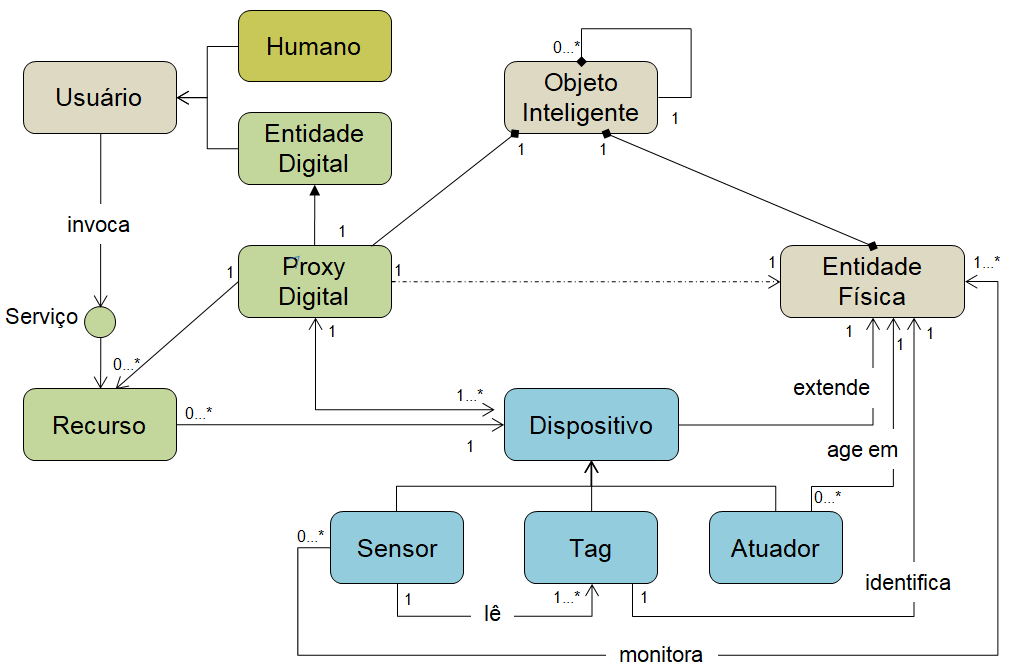
\includegraphics[width=0.9\linewidth]{chapters/background/arquitetura_IoT.png}
	\caption{Modelo de Referência para IoT. Fonte:~\cite{serbanati:2011}}
	\label{fig:modeloiot}
\end{figure}

Assim,~\cite{serbanati:2011} apresentam um modelo de referência para IoT (Figura~\ref{fig:modeloiot}) que define ``Entidades Físicas'' e ``Entidades Digitais'', onde as entidades físicas podem ser quaisquer objetos ou ambientes (de humanos a dispositivos eletrônicos ou ambientes fechados/abertos) discretos e identificáveis que sejam de interesse do usuário e o ajudem a alcançar a sua própria meta, e as digitais são ``entidades de \textit{software} que podem ser agentes com objetivos autônomos, serviços ou entradas de dados coerentes''. Além disso, as entidades digitais podem interagir tanto entre si quanto com os usuários e, no mundo digital, podem representar entidades físicas, nesse caso, como um ``\textit{Proxy} Digital''.

\cite{serbanati:2011} esclarecem que as representações digitais de Entidades Físicas podem ser de diversos tipos, dentre eles: modelos 3D, avatares, objetos (ou instâncias de uma classe em uma linguagem de programação orientada a objetos) e, até mesmo uma conta de rede social pode ser vista como tal. Entretanto, no contexto da IoT, de acordo com~\cite{serbanati:2011}, Proxies Digitais tem duas propriedades fundamentais:

\begin{itemize}
	\item Cada \textit{Proxy Digital} \textbf{representa biunivocamente uma única Entidade Física} e, por isso, contém apenas um ID para identificar o objeto representado. Além disso, a associação entre o Proxy Digital e a Entidade Física representada deve ser estabelecida automaticamente;
	\item Um \textit{Proxy Digital} é uma \textbf{representação sincronizada de um conjunto de propriedades da Entidade Física}. Assim, os parâmetros digitais relevantes que representam as características da Entidade Física podem ser atualizados de acordo com qualquer mudança observada no estado da entidade física (i.e.: através de sensores). De modo análogo, as alterações que afetam o Proxy Digital podem se manifestar na Entidade Física (i.e.: através de atuadores).
\end{itemize}

A extensão de uma Entidade Física e do \textit{Proxy} Digital associado a ela é definida por~\cite{serbanati:2011} como ``\textit{Objeto Inteligente}'', sendo necessário que \textit{Dispositivos} façam essa integração de modo que ``quaisquer mudanças nas propriedades de um objeto inteligente devem ser representadas tanto no mundo físico quanto no digital''.

Assim, do ponto de vista funcional, tais Dispositivos podem ser de três tipos: (i) \textbf{Sensores}, que proveem informações sobre a Entidade Física que eles monitoram; (ii) \textbf{Tags} (código de barra, QRCode, RFID,...), que podem dar suporte ao processo de identificação; e, (iii) \textbf{Atuadores}, que podem modificar o estado físico da Entidade Física. 

Além dos componentes mencionados anteriormente, no Modelo de Referência para IoT apresentado na Figura~\ref{fig:modeloiot}, podem ser observados outros dois elementos: (a) ``Recurso'' e (b) ``Serviço''. Onde, Recursos são componentes digitais que podem prover cinco capacidades diferentes: (1) recuperação ou modificação das propriedades físicas de uma Entidade Física associada, por meio de sensores ou atuadores; (2) modificação ou recuperação de propriedades digitais de um Proxy Digital associado; e (3) uso de serviços de hardware complexo ou de software através do objeto inteligente associado. E, por fim, Serviço é o meio pelo qual os recursos são efetivamente acessados para minimizar a dependência que as implementações tem em relação ao  \textit{hardware}.

É importante salientar que, no contexto deste trabalho, o uso de elementos de IoT diz respeito às relações e às interações que os componentes físicos e digitais precisam estabelecer e que são expressas através de modelos computacionais já estabelecidos como os apresentados nos trabalhos de~\cite{Chang:2014} e~\cite{serbanati:2011}.

% \subsection{Sistemas multiagente}
% Segundo~\cite{bez:2012}, sistemas multiagente são sistemas com múltiplos agentes com (i) comportamento autônomo e que (ii) interagem uns com os outros, sendo essas, suas duas características básicas. Além disso, cada agente é um elemento autônomo que trabalha independentemente dos outros agentes, assim, um sistema multiagente é um sistema computacional que coordena as habilidades dos diversos agentes individuais para resolver problemas ou satisfazer um conjunto de tarefas ou objetivos~\citep{bez:2012}.

% No que diz respeito à categorização, existem dois tipos de sistemas multiagente: reativo e cognitivo. Os sistemas do tipo reativo apenas respondem a estímulos ambientais, sem qualquer tipo de modelo do ambiente ou memória das ações e possuem grande número de agentes. O sistemas cognitivos tem poucos agentes, pois, cada agente é um sistema complexo e computacionalmente caro. Nesses sistemas, os agentes raciocinam e deliberam em conjunto quais ações ou planos devem ser executados e quais objetivos serão alcançados, além de manter históricos das interações passadas~\citep{giuffra:2012,ferber:1991}. 

% Em um ambiente de aprendizagem que também tenha, por exemplo, ciência de contexto, um sistema multiagente será o responsável pela percepção das sensações ambientais, reconhecimento de determinado estado do usuário e deliberação das recomendações ou ações que gerem adaptações que permitam personalização da experiência de ensino-aprendizagem. Os trabalhos inicialmente encontrados nessa área e aplicados à educação digital não utilizavam sistemas multiagente em sistemas ciber-físicos para intervenção e adaptação de conteúdo no decorrer do processo educacional.

\subsection{Sistemas Ciberfísicos}\label{section:ciberfisico}
O termo ``sistemas ciberfísicos'' foi proposto por Helen Gills para definir sistemas físicos, biológicos e de engenharia, cujas operações são integradas, monitoradas e/ou controladas por um núcleo computacional e os seus componentes estão conectados~\citep{wade:2015}. Esse termo está substituindo o famoso ``Sistemas Embarcados'', pois, enfatiza de modo mais evidente sua interação com o mundo físico~\citep{helps:2013}.

Segundo~\cite{chase:2011}, por estarem diretamente conectados ao ambiente físico, sistemas ciberfísicos tem como principais características: (i) confiáveis: não podem falhar; (ii) seguros: não pode causar dano ao ambiente e à vida que nele habita (iii) restrição de tempo: processamento de dados dentro de um pequeno limite temporal, pois, as notificações e tomadas de decisões, em determinadas circunstâncias, precisam ser imediatas.

Diversos trabalhos usando sistemas ciberfísicos tem surgido a partir das necessidades de melhoria nos processos de ensino-aprendizagem, ora focando no ensino de Engenharia, ora focando em aprendizagem colaborativa e ambientes adaptativos ou ainda na criação de extensões de ambientes virtuais~\citep{Santos:2014,lei:2013,wade:2015,noor:2011,pester:2015,peter:2015}.

Assim, tendo enfoque na construção de um ambiente ciberfísico de aprendizagem, \cite{santos:2014ambientes} propõe oito requisitos para a construção desses ambientes: (i) prover \textbf{comunicação e interação} entre estudantes e professores com vistas a possibilitar a aprendizagem colaborativa; (ii) possuir \textbf{ferramentas administrativas} para gerência educacional; (iii) possuir \textbf{ferramentas de avaliação} da aprendizagem; (iv) possibilitar diferentes \textbf{abordagens pedagógicas}; (v) possuir \textbf{ferramentas de autoria} que possibilitem a criação ou edição de conteúdos educacionais; (vi) possuir algum nível de \textbf{inteligência} para o auxílio da aprendizagem; (vii) proporcionar maior \textbf{engajamento} através de experiências participativas; (viii) deve ter uma \textbf{abordagem multissensorial} que integre informações dos ambientes, tais como sons, vídeos, textos e animações 3D, entre outras.

No contexto desta teste, um sistema ciberfísico implica na inserção e utilização de objetos de aprendizagem que sejam simultaneamente físicos e digitais em um ambiente de aprendizagem tal como outros objetos tradicionais, i.e. slides, vídeos, imagens, simulações, entre outros, o que implica na necessidade de mecanismos de controle (atuadores) e de percepção (sensores). Além disso, o ambiente de aprendizagem deve possibilitar coleta de dados de interação dos alunos durante a utilização desses objetos tangíveis e deve fornecer instrumentos para posterior análise dos dados, avaliação/acompanhamento da aprendizagem e propostas de intervenção pedagógica nos processos de ensino-aprendizagem dos estudantes.


% No contexto desta proposta, após a aula, um sistema ciber-físico pode recomendar atividades pedagógicas com objetos de aprendizagem físico-virtuais levando em consideração as dificuldades específicas de um aluno, percebidas pelo sistema, com relação a algum aspecto do conteúdo didático. Nenhum dos trabalhos encontrados que utilizam sistemas ciber-físicos em contextos educacionais utilizavam uma abordagem muiltiagente aliada a análise de dados educacionais dos alunos para tomada de decisões no sentido de adaptar conteúdo educacional ao estilo de aprendizagem ou à necessidade de reforço didático do estudante.
	
	
% \subsection{Ambientes de Sala de aula inteligente}

% Enquanto ~\cite{Gligoric:2012} considera que uma sala de aula inteligente é uma sala de aula que provê, em tempo real, \textit{feedback} automático, por exemplo, sobre a qualidade da aula, podendo também ser um ambiente inteligente equipado com diferentes tipos de \textit{hardware} e \textit{software}, para~\cite{Bargaoui:2014}, o que caracteriza esses ambientes é o fato de eles serem projetados de modo a permitir o controle dos equipamentos audiovisuais, computadores, projetores, lousas interativas com o objetivo de facilitar a interação entre professores e alunos.

% Assim, a leitura de diversos trabalhos relacionados, aponta para a percepção de que uma sala de aula inteligente é caracterizada pela inserção de dispositivos computacionais como \textit{tablets}, lousas inteligentes ou sensores diversos que possibilitem maior interatividade e algum nível de inferência para recomendações ou notificações ao professor ou ao aluno, utilizando elementos de computação pervasiva ou Internet das Coisas~\citep{Margetis:2011,Santana:2013,Dekdouk:2012}.

% Outra interpretação de sala de aula inteligente pode ser feita a luz de trabalhos focados na construção de Ambientes Virtuais de Aprendizagem (AVA). Assim, alguns dos trabalhos relacionados a AVA apresentam arquiteturas e implementações, baseadas em tecnologia Web ou de dispositivos móveis, para proporcionar interação virtual entre os alunos~\citep{Monteiro:2015} ou ambientes de aprendizagem colaborativa~\citep{Brito:2002,Netto:2003}.

% %Se a inserção de recursos computacionais tem como objetivo principal apoiar e facilitar os processos de ensino-aprendizagem e, assim, garantir uma maior qualidade na educação, então, uma sala de aula inteligente não pode ser esquivar de levar em consideração o modo retemos conhecimento.

% %\begin{figure}[h]
% %	\centering
% %	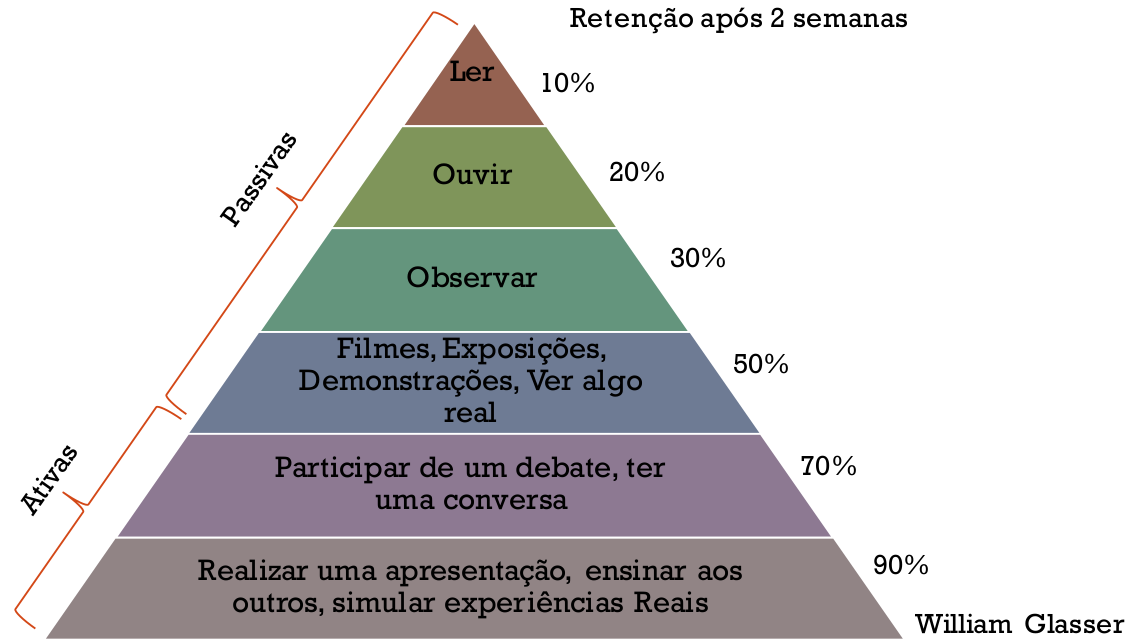
\includegraphics[width=0.7\linewidth]{imgs/piramide_glasser}
% %	\caption{Como aprendemos - Pirâmide de Glasser}
% %	\label{fig:piramide_glasser}
% %\end{figure}

% %  Conceito de sala de aula inteligente, possibilidades de aquisição de dados de sensores, dados de interação com o conteúdo educacional, possibilidades de inferências, recomendações ou notificações com relação às dificuldades ou potencialidades da turma ou de um aluno específico.
% %
% %Apresentar elementos sobre retenção de conhecimento a partir da pirâmide de William Glasser (apresentação do Tiago Primo) e como a educação apoiada por tecnologia pode ajudar nisso(quanto mais ativa aprendizagem, mais conhecimento é retido). Apresentar o conceito de sala de aula inteligente como um caminho para maior engajamento do estudante e retenção quando unido com atividades de aprendizagem ativa.



\subsection{Interfaces Tangíveis de Usuário}\label{section:TUI}

\cite{ishii:1997} introduziram o conceito de ``Interfaces Tangíveis de Usuário'' (do inglês, \textit{Tangible User Interfaces} - TUIs) como um novo tipo de Interface Humano-Computador (IHC) que permite ao usuário interagir com um sistema computacional através de objetos e ambientes físicos do dia-a-dia, ao invés de utilizar periféricos tradicionais como mouse, teclado e monitor em conjunto com uma Interface Gráfica de Usuário - GUI (Figura~\ref{fig:guiandtui}).

\begin{figure}[htb]
	\centering
	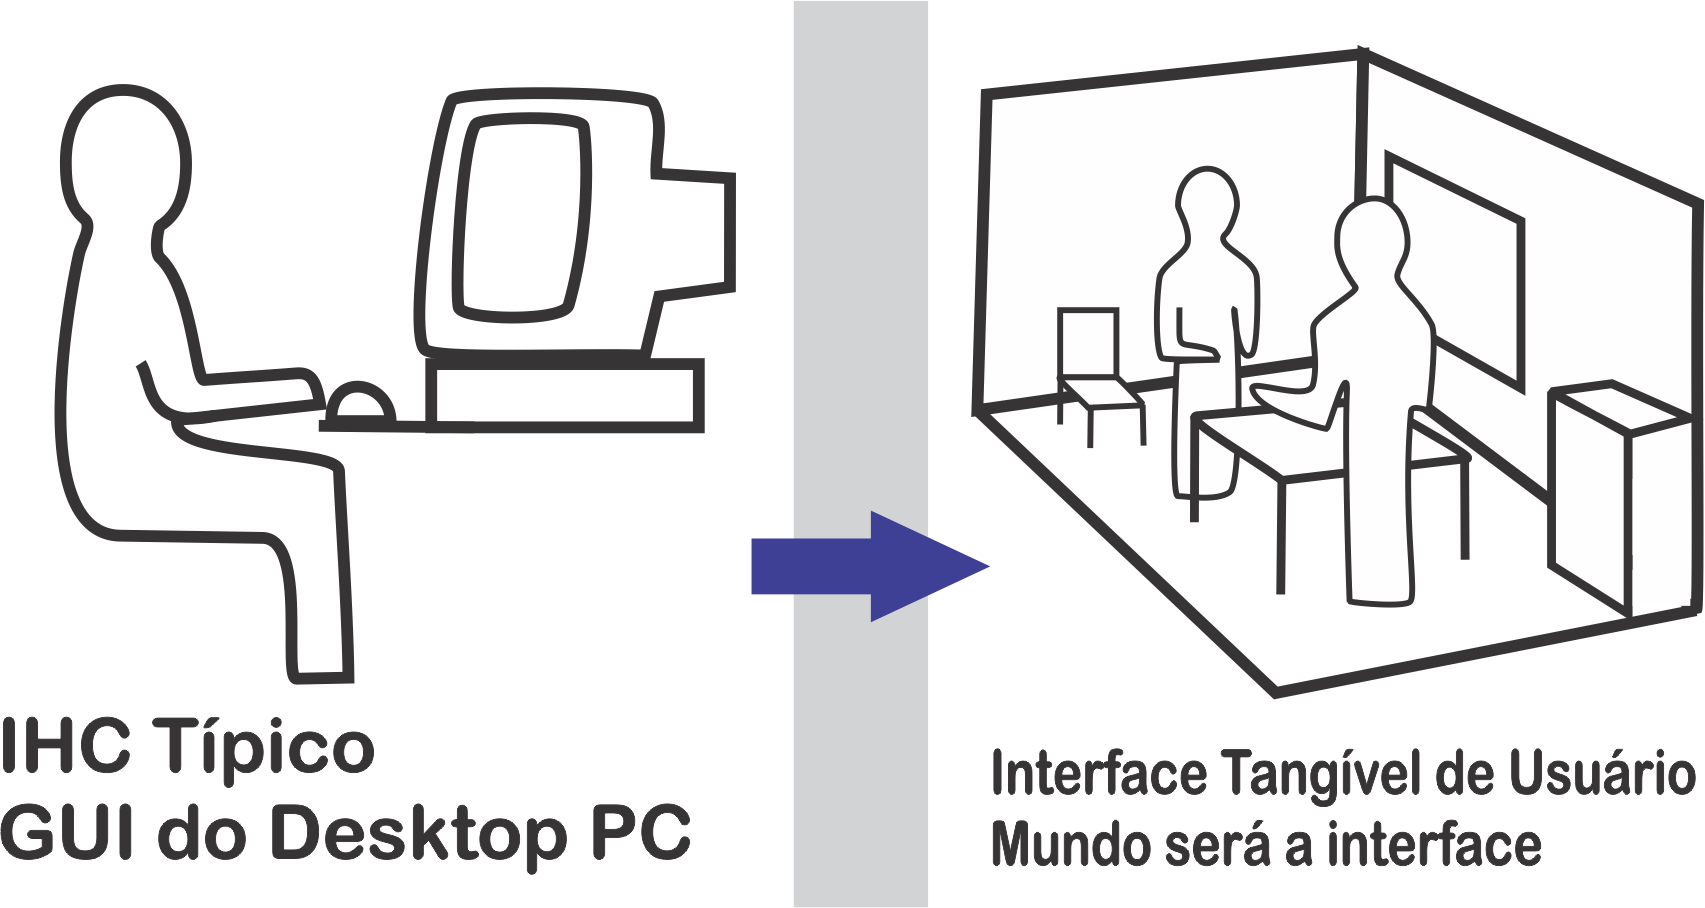
\includegraphics[width=0.7\linewidth]{chapters/background/GUIandTUI_redesenhado.png}
	\caption{GUI e TUIs. Fonte:~\cite{ishii:1997}}
	\label{fig:guiandtui}
\end{figure}

Segundo \cite{ullmer:2000}, interfaces tangíveis de usuário dão forma física à informação digital de modo que os objetos físicos servem como representações ou controles físicos para a mídia computacional. Assim, essas representações físicas (tangíveis) são combinadas com representações digitais (intangíveis e transitórias) resultando em sistemas fisicamente interativos, mas, mediados computacionalmente. Para um melhor entendimento, \cite{ullmer:2000} fornecem a seguinte heurística: quando a força/energia de uma interface tangível é desligada, as representações digitais desaparecem e as representações físicas persistem, de modo que ``as interfaces tangíveis são produtos de um cuidadoso equilíbrio entre essas duas formas de representação''.

\begin{figure}[htb]
	\centering
	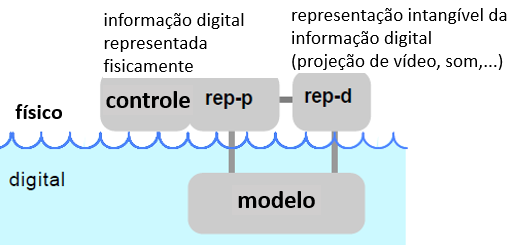
\includegraphics[width=0.6\linewidth]{chapters/background/MCRpd_2.png}
	\caption{Modelo de interação de TUI - MCRpd. Fonte:~\cite{ullmer:2000}}
	\label{fig:MCRpd}
\end{figure}

Assim, baseando-se no padrão que serviu de modelo tradicional para construção de interfaces gráficas de usuário (\textit{model-view-controller}), onde a interação humana acontece basicamente através de `entrada' (por meio de periféricos como mouse e teclado) e `saída' (representações digitais como gráficos e texto baseados em tela), \cite{ullmer:2000} apresentam um modelo de interação para interfaces tangíveis que denominam de \textit{model-control-representation (physical and digital)} (MCRpd), onde os elementos ``modelo'' e ``controle'' são mantidos e o elemento \textit{view} foi dividido em dois subcomponentes: representações físicas (``rep-p'') e representações digitais (``rep-d''), conforme a Figura~\ref{fig:MCRpd}.

Segundo~\cite{ullmer:2000} e~\cite{zhou:2015}, o modelo de interação intangível destaca quatro características chave das interfaces tangíveis: 
\begin{enumerate}
	\item As representações físicas (`rep-p') são acopladas computacionalmente aos dados digitais subjacentes (`modelo')
	\item As representações físicas incorporam mecanismos de controle físicos interativos (`controle'), permitindo ao usuário a manipulação de objetos.
	\item As representações físicas são acopladas perceptivamente às representações digitais (`rep-d').
	\item O estado físico dos objetos tangíveis incorpora parcialmente o estado digital do sistema, de modo que, o sistema é, pelo menos, parcialmente legível se a energia for cortada.
\end{enumerate}

%Objetos tangíveis são acoplados a dados digitais por meio de funcionalidade computadorizada.
%Interação manual com objetos tangíveis: os objetos tangíveis incorporam os meios de controle interativo, permitindo ao usuário manipular objetos.
%Os objetos tangíveis são acoplados perceptivamente com a representação produzida digitalmente.
%O estado dos objetos tangíveis incorpora aspectos centrais do estado de todo o sistema (significado representacional), e o sistema é, portanto, pelo menos parcialmente legível se a energia for cortada.

\textbf{Interfaces Tangíveis na Educação}

No últimos anos, diversos trabalhos tem apresentado interfaces tangíveis aplicadas ao ensino-aprendizagem, assim foram propostos principalmente trabalhos envolvendo mesas tangíveis \citep{mendoza:2019, ishii:1997}, blocos para programação tangível \citep{panaggio:2019, carbajal:2018, leite:2017, viana:2018}, realidade aumentada \citep{imamura:2018}, realidade virtual \citep{gluz:2018, lopes:2018}, aprendizado de habilidades espaciais~\citep{ha:2018}, disciplinas STEM \citep{Azad:2016} ou do currículo comum \citep{Blikstein:2012, Blikstein2016} e ferramentas de apoio a estudantes com dificuldade de comunicação \citep{moreira:2018, moreira:2018b}

Além disso, \cite{zuckerman:2005} apontam que objetos tangíveis podem ser úteis para ensinar conceitos abstratos e apresenta três vantagens para seu uso: (i) engajamento sensorial (toque, visão e audição), (ii) acessibilidade e (iii) aprendizagem em grupo. \cite{marshall:2007} ao questionar sobre se objetos tangíveis melhoram o aprendizado sugere que entre os possíveis benefícios estão: (i) se percepção e cognição estão interligados, então, o uso de materiais tangíveis no contexto de aprendizagem pode ser mais eficiente do que o simples uso de representação visual;  (ii) a ligação entre a ação física (manipulação) e seus efeitos digitais pode levar a um maior engajamento e reflexão por parte dos estudantes; (iii) interfaces tangíveis podem ser particularmente adequadas para aprendizagem colaborativa, uma vez que podem ser projetadas para proporcionar um espaço compartilhados de atividades colaborativas.

No contexto desta tese, interfaces tangíveis de usuário são objetos de aprendizagem com as características apresentadas por \cite{ullmer:2000} e \cite{zhou:2015} no que diz respeito a interação/acoplamento das representações físicas e digitais e que, nesta proposta, tem sua estrutura e funcionamento formais definidos como um objeto inteligente conforme previsto no modelo de referência para IoT proposto por \cite{serbanati:2011}, isto é, contendo entidades físicas e digitais interligadas, além de dispositivos, recursos e serviços.

\subsection{Ferramentas de Autoria de OAs}\label{section:ferramentasautoria_avaliacao}
A inserção e o uso de objetos de aprendizagem supõe, num momento anterior, a criação de tais objetos. Para isso, são utilizadas ferramentas de autoria, que permitem ao autor de um objeto, mesmo sem profundos conhecimentos de informática, criar materiais educacionais através de manipulação, desenvolvimento e uso de objetos de aprendizagem (OA)~\citep{Flores:2011}.

Desse modo, na literatura, podem ser encontradas diversas abordagens e metodologias que propõem tanto novas ferramentas para criação de objetos de aprendizagem~\citep{Orlandi:2012,Flores:2011} quanto o uso de \textit{softwares} consolidados no mercado e, por isso, de fácil acesso~\citep{Passos:2010}. Além disso, para melhor contribuir com a qualidade da aprendizagem, uma ferramenta de autoria precisa ser adequada a criar OAs contextualizados, por isso, baseando-se em~\cite{Kolb:2014},~\cite{Gagne:2013} e ~\cite{Wiley:2000},~\cite{Flores:2011} define um conjunto de funcionalidades que precisam estar presentes em uma ferramenta de autoria para a construção de OAs contextualizados (Tabela~\ref{Tabela:Objetos de Aprendizagem}).

Neste trabalho, propomos a modificação do módulo ``Compositor'', que é a ferramenta de autoria de OAs apresentada na pesquisa de mestrado de ~\cite{leitao:2017} e está integrada a plataforma de educação digital do Grupo de Interesse em Sistemas Embarcados. Tal modificação deverá permitir a criação e a inserção de objetos tangíveis de aprendizagem, isto é, que utilizem ao mesmo tempo manipulativos físicos e digitais no contexto educacional.

\begin{table}[htbp]
	\caption{Funcionalidades dos OAs em uma ferramenta de autoria}
	\begin{tabular}{|l|l|}
		\hline
		\multicolumn{1}{|c|}{\textbf{FUNCIONALIDADE}} & \multicolumn{1}{c|}{\textbf{DESCRIÇÃO}} \\ \hline
		Applet Java & Permite o uso de aplicativos desenvolvidos em Java como \\ &simulações, jogos, animações, vídeos, modelos 3D \\ \hline
		Apresentação de Slides & Permite inserir apresentações de slides no OA \\ \hline
		Leituras & Permite disponibilizar textos que servirão como embasamento e \\ &orientação sobre o assunto do OA. \\ \hline
		Estudo de Caso & Permite simular determinada situação problema, com possíveis \\ &cenários, atores e fatos \\ \hline
		Atividades com Texto Livre & Permite incluir textos livres com informações gerais, instruções, \\ &exemplos, curiosidades, leituras, sobre o assunto do OA.  \\ \hline
		Feeds (ou feed RSS) & Permite seleção de \textit{sites} que tratam de assuntos ligados ao \\&do OA.  \\ \hline
		Site da Web & Permite colocar links para sites relacionados com o tema \\&do OA. \\ \hline
		Galeria de Imagens & Permite colocar várias imagens para ilustrar o conteúdo. \\ \hline
		Ampliação de Imagens & Permite ampliar uma imagem para investigar suas \\&características. \\ \hline
		Objetivo & Permite descrever o resultado de aprendizagem esperado \\ &quando os alunos tiverem concluído a atividade.  \\ \hline
		Pré-requisitos & Permite descrever os conhecimentos prévios necessários \\ &para que os alunos possam completar efetivamente sua \\ &aprendizagem. \\ \hline
		Questionário & Permite criar questões que visam melhorar o desempenho do \\ &aluno. O professor poderá elencar dicas e \textit{feedback} para cada \\ &uma das questões. \\ \hline
		Questões Múltipla Escolha & Permite criar questões objetivas com apenas uma resposta \\&correta. \\ \hline
		Questão de Seleção Múltipla & Permite criar questões de múltipla escolha com duas ou mais \\ &respostas corretas. \\ \hline
		Questão Verdadeiro-Falso & Permite criar questões que apresentem uma declaração a ser \\ &analisada, para que o aluno determine se ela é verdadeira \\&ou não. \\ \hline
		Exercícios Cloze & Permite criar questões em forma de texto ou frases em que o \\ &aluno deve preencher as lacunas com as palavras que faltam. \\ \hline
		Reflexão & Permite criar questões que dão oportunidade aos alunos de \\ &observar e refletir sobre suas observações. \\ \hline
		Completar & Permite criar questões para serem completas com palavras: \\ &arrastando os textos, ou selecionando, ou escrevendo. \\ \hline
	\end{tabular}
	\label{Tabela:Objetos de Aprendizagem}
\end{table}


\subsection{Avaliação da Aprendizagem}\label{section:avaliacao_aprendizagem}

Embora, os exames escolares da forma como os conhecemos hoje foram sistematizados a cerca de 500 anos, de acordo com~\cite{luckesi:2014}, a expressão `avaliação da aprendizagem' começou a ser utilizada em 1930 por Ralph Tyler para falar do cuidado que os educadores precisam ter com a aprendizagem dos seus educandos em um contexto histórico que de 100 crianças, somente 30 eram aprovadas anualmente.

Assim, segundo~\cite{luckesi:2014}, Tyler propôs um sistema de `ensino por objetivos' o que implicou em estabelecer com precisão o que os estudantes deveriam aprender e o que o professor deveria fazer para que isso acontecesse. Tal sistema era composto de 4 passos básicos com coisas que o professore deveria executar~\citep{luckesi:2014}: (i) ensinar alguma coisa; (ii) diagnosticar sua consecução; (iii) caso a aprendizagem fosse satisfatória, seguir em frente; (iv) caso não fosse satisfatória, reorientar tendo em vista o objetivo que é obter um resultado satisfatório. Embora antigo, simples e até óbvio,~\cite{luckesi:2014} afirma que essa proposta nunca foi efetivamente abraçada pelos meios educacionais.

Além disso,~\cite{luckesi:2002} faz uma diferenciação entre `exame' e `avaliação' escolar onde afirma ser um equívoco tratar as duas coisas como sinônimos. Assim, avaliar seria o `ato de diagnosticar uma experiência' com o intuito de reorientá-la para produzir o melhor resultado possível, não sendo classificatória, nem seletiva, mas, diagnóstica e inclusiva. Enquanto isso, para ele, examinar por ser classificatório e seletivo, é também excludente e tem seu centro no julgamento de `aprovado' ou `reprovado'.

Embora seja um diagnóstico passível de ser registrado como uma nota, um valor quantitativo, a avaliação é mais no sentido de atribuir uma qualidade a algo, logo, ela é essencialmente qualitativa~\citep{luckesi:2002}. Desse modo, alguém que acerta 03 questões de um total de 10 em um exame, significa apenas uma quantidade, isto é, a pessoa acertou 30\% das questões. Entretanto, a avaliação acontece ao atribuir uma qualidade a esse fato, tal qualidade pode ser positiva ou negativa. Assim, a qualidade é atribuída a partir de uma quantidade, sobre o que~\cite{luckesi:2002} chama de `contagem de frequências'.

Por conseguinte, a avaliação da aprendizagem deve ser encarada mais como um instrumento para melhoria nos processos de ensino e de tomada de decisão dos caminhos e trilhas a seguir do que uma simples como uma instância de verificação ou aferição~\cite{luckesi:2014}. Assim, o ato de avaliar a aprendizagem deve ser visto mais como um processo que ajuda a direcionar o aprendizado e o desenvolvimento dos estudantes do que um ato de verificação com o objetivo de aprovar ou reprovar permeado de opressão e medo.

Com relação a avaliação do desempenho dos alunos ao longo dos processos de ensino-aprendizagem são encontradas abordagens que simplesmente inserem cálculos tradicionais de pontuação~\citep{Orlandi:2012}, mas, há ainda propostas de ferramentas que utilizam dados provenientes da interação com o material didático ou da participação do aluno em atividades virtuais como fóruns, bate-papos, etc~\citep{Lucena:2015, Nunes:2016, Malvezzi:2010}. Tais trabalhos serão melhor analisados e descritos na Seção~\ref{sec:avaliacao}. 

Adicionalmente, uma vez que os objetos físicos-digitais podem ser utilizados para coletar dados de interação dos alunos com o material pedagógico, a Seção~\ref{section:analytics} deste trabalho propõe algumas métricas que visam fornecer mais elementos que auxiliem no processo de avaliação da aprendizagem dos estudantes.


% -----------------------------------------------------------------
% => Summary - BACKGROUND - 2
% -----------------------------------------------------------------
\section{Resumo}
% \label{summary:background}

Este capítulo descreveu os principais conceitos para o entendimento deste trabalho. Assim, na Seção~\ref{section:educacao_praticas} foram introduzidos conceitos e discussões sobre educação e fracasso escolar, além da necessidade de modificações das práticas pedagógicas visando maior êxito dos atores envolvidos nesse processo. %Nessa seção, também foram introduzidos elementos relacionados ao processo de ensino-aprendizagem e ao paradigma construcionista. 

Na Seção~\ref{section:sociopedagogicas} foram brevemente apresentadas as teorias de John Dewey, Paulo Freire, Jean Piaget e Lev Vygotsky que serviram de base para o desenvolvimento da abordagem proposta nesta tese. 
%Além disso, foi feita uma explanação do Construcionismo em oposição a abordagem Instrucionista, onde é apontado como o Construcionismo rompe com o modelo tradicional de educação no qual o processo de ensino-aprendizagem é tido como mera transmissão de conhecimento e o professor como único ou maior detentor deste conhecimento.

Na Seção~\ref{section:computacao_educacao} foram apresentados conceitos relacionados à inserção da computação na Educação, assim, foram abordados temas como %Aprendizagem Ubíqua, Inteligência de Ambientes, Ciência de Contexto, 
Objetos de Aprendizagem, Internet das Coisas, Sistemas Ciberfísicos, Interfaces Tangíveis de Usuário, 
% Ambientes de Sala de Aula Inteligente, 
Ferramentas de Autoria e de Avaliação da Aprendizagem. 
% que são muito utilizados no projeto e implementação de salas de aula inteligentes.


% -----------------------------------------------------------------
% => RELATED WORKS - 3 [DOING]
% -----------------------------------------------------------------
%% 
% -----------------------------------------------------------------
% => RELATED WORKS
% -----------------------------------------------------------------

\chapter{Trabalhos Correlatos} \label{Chap:relatedWork}

% Este capítulo apresenta e discute os principais trabalhos existentes na literatura e que se relacionam com esta proposta de Tese. Por essa razão, as pesquisas abordadas a seguir são propostas de desenvolvimento de ambientes de sala de aula com inserção de novas tecnologias, isto é, ambientes de sala de aula inteligente (do inglês, \textit{smart classroom}). Além disso, são apresentados também trabalhos relacionados a autoria de objetos de aprendizagem e avaliação do desempenho dos estudantes em aulas apoiadas por tecnologia.

Este capítulo apresenta e discute os principais trabalhos existentes na literatura e que se relacionam com esta Tese. Por essa razão, as pesquisas abordadas a seguir são propostas de utilização de sistemas ciberfísicos no contexto educacional (Seção~\ref{sec:ciberfisicos}). Além disso, a integração desses sistemas ao processo educacional como um todo, isto é, ao planejamento, execução e avaliação do ensino-aprendizagem implica não apenas na construção de objetos de aprendizagem que sejam tangíveis (físico-digitais), mas, ainda, na necessidade de ferramentas de autoria e utilização desses objetos (Seção~\ref{sec:autoria}), além de ferramentas de avaliação da aprendizagem dos estudantes em aulas apoiadas por tecnologia (Seção~\ref{sec:avaliacao}).

\section{Sistemas Ciberfísicos na Educação}
\label{sec:ciberfisicos}

%O uso de sistemas ciberfísicos no contexto educacional tem sido objeto de diversas pesquisas nos últimos anos, onde alguns estudos apenas implementam manipulativos físicos e virtuais em separado com a finalidade de realizar comparações~\citep{zacharia:2011, Salehi:2014}, outros trabalhos mais recentes utilizam manipulativos híbridos (físico-virtuais)~\citep{ha:2018, Azad:2016} ou utilizam físicos e virtuais concomitantemente~\citep{Blikstein:2012, Blikstein2016}. De modo geral, o que se tem notado é que a associação entre o físico e o virtual tende a ajudar mais os processos de aprendizagem dos estudantes do que a utilização exclusiva de apenas um tipo de manipulativo. %Além disso, apenas o trabalho de~\cite{Santos:2014} foi encontrado em publicações vinculadas ao Congresso Brasileiro de Informática na Educação (CBIE).

O uso de manipulativos no contexto educacional tem sido objeto de diversas pesquisas nos últimos anos, onde alguns estudos investigam o uso de manipulativos físicos e virtuais em separado com a finalidade de realizar comparações~\citep{zacharia:2011, Salehi:2014}, outros trabalhos mais recentes utilizam manipulativos tangíveis (físico-digitais)~\citep{ha:2018, Azad:2016} ou utilizam físicos e virtuais concomitantemente~\citep{Blikstein:2012, Blikstein2016}. De modo geral, o que se tem notado é que a associação entre o físico e o virtual tende a ajudar mais os processos de aprendizagem dos estudantes do que a utilização exclusiva de apenas um tipo de manipulativo. %Além disso, apenas o trabalho de~\cite{Santos:2014} foi encontrado em publicações vinculadas ao Congresso Brasileiro de Informática na Educação (CBIE).

Antes de prosseguirmos, é importante salientar que, neste texto, o termo Manipulativo Virtual (MV) refere-se ``a visualizações dinâmicas virtuais interativas de aparelhos e materiais, fornecidas por meio de uma simulação computacional (laboratório virtual)'', conforme apresentado por \cite{zacharia:2011}, de modo que a experiência de aprendizagem acontece através da interação/manipulação de um material totalmente virtual que simula o mundo físico. Além disso, Manipulativo Físico (MF) é um objeto de aprendizagem de interação manual sem qualquer nível de conectividade computacional e Manipulativo Tangível (ou físico-digital) corresponde aos objetos apresentados na seção~\ref{section:TUI}.

\subsection{Manipulativos Físicos \textit{versus} Manipulativos Virtuais}

\textbf{Aprendizado de Física}\\
~\cite{zacharia:2011} realizaram experimentos para comparar se a utilização de manipulativos físicos (MF) e virtuais (MV) tem algum diferencial no aprendizado de Física no Ensino Superior. Os experimentos são realizados em quatro cenários: (i) apenas MF; (ii) apenas MV; (iii) MF precedendo MV e; (iv) MV precedendo MF. Além disso, os efeitos da manipulação física ou virtual na compreensão dos estudantes acerca dos conceitos de calor e temperatura foram examinados e comparados a educação tradicional (modo passivo de instrução).

Para a condução dos experimentos, foi utilizado um laboratório real de física para o experimento com MF e o \textit{software ``Virtual Lab ThermoLab''} (Figura~\ref{fig:zacharia_thermolab}) para o experimento com MV. Participaram do estudo 234 universitários inscritos em um curso introdutório de física, sendo 55 do sexo masculino e 168 do sexo feminino e tendo uma média de idade de 18.5 anos. Estes estudantes foram divididos em grupos menores de acordo com os cenários já mencionados.

\begin{figure}[htb]
	\centering
	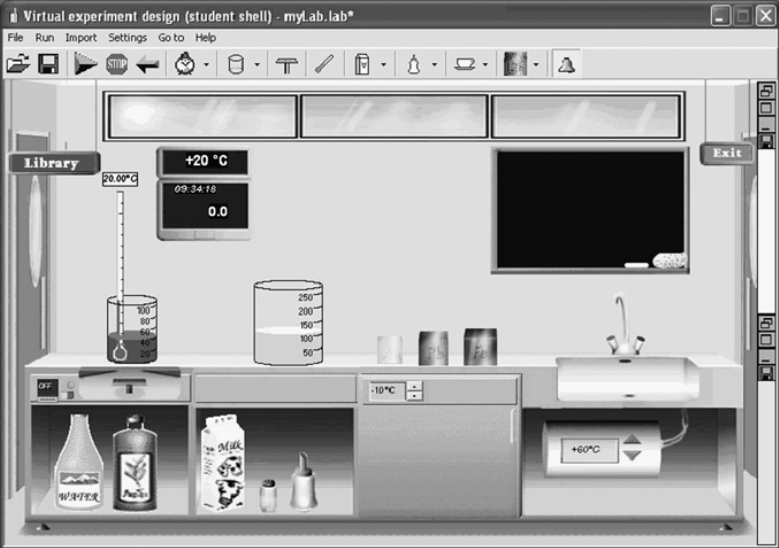
\includegraphics[width=0.90\linewidth]{chapters/works/zacharia2011.png}
	\caption{ThermoLab. Fonte:~\cite{zacharia:2011}}
	\label{fig:zacharia_thermolab}
\end{figure}

Foram realizadas quatro sessões experimentais com pré e pós-testes, onde cada teste continha 4 questões abertas e, um teste final com 8 questões abertas. Além disso, segundo os autores, não haviam itens idênticos entre o teste final e o resto dos testes e, para pontuação, foram consideradas se as respostas e as explicações das mesmas estavam certas ou erradas, onde uma resposta correta valia um ponto, e cada explicação correta valia meio ponto (uma questão poderia ter mais de uma explicação).

Com relação aos resultados, o estudo concluiu que, de modo geral, o uso de manipulativos pode contribuir tanto ou mais do que o ensino tradicional para o entendimento dos conceitos de calor e temperatura. Além disso, embora não tenham sido encontrados indícios de que o uso de manipulativos físicos é pré-requisito para o aprendizado de física, os achados corroboram que a manipulação é importante, seja ela física ou virtual. Outra descoberta diz respeito a combinação entre MF e MV, onde não foram encontradas diferenças entre iniciar com uma abordagem e prosseguir com outra ou trabalhar inteiramente com apenas uma delas.

Por fim, embora o trabalho de~\cite{zacharia:2011} tenha proposto a comparação entre o uso de objetos de aprendizagem físicos e virtuais, em nenhum dos casos há coleta de dados de interação dos estudantes com o material didático. Além disso, a experimentação envolvendo objetos físicos e virtuais mantém os dois tipos em separado, isto é, apenas físico e apenas virtual, adicionando apenas a opção metodológica de um ou outro e o seu uso consecutivo. Entretanto, um ganho importante é a evidência de que o uso de manipulativos físicos ou virtuais melhora a aprendizagem dos estudantes.

\textbf{Aprendizado de Eletrônica}\\
\cite{Salehi:2014} apresentam um estudo de menor porte, mas similar ao estudo de~\cite{zacharia:2011}, que avalia os efeitos do uso de manipulativos físicos e virtuais no aprendizado de conceitos básicos de eletrônica, mais precisamente de circuitos elétricos em série e paralelo, de acordo com as imagens apresentadas na Figura~\ref{fig:salehi2014}.

%\begin{figure}[htb]
%	\centering
%	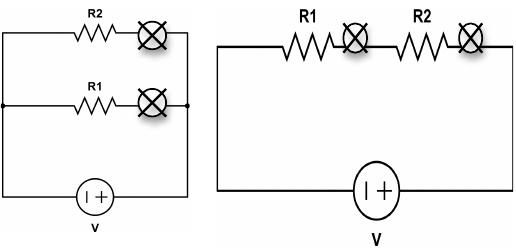
\includegraphics[width=0.6\linewidth]{imgs/salehi2014_circuito.png}
%	\caption{Esquema dos circuitos usados no estudo. Fonte:~\cite{Salehi:2014}}
%	\label{fig:salehi2014_circuitos}
%\end{figure}


\begin{figure}[htb]
	\center
	\subfigure[ref1][Manipulativo Físico]{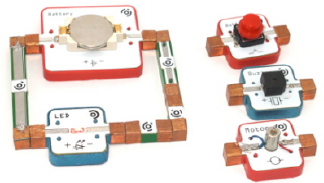
\includegraphics[width=7cm]{chapters/works/salehi-1.png}}
	\qquad
	\subfigure[ref2][Manipulativo Virtual]{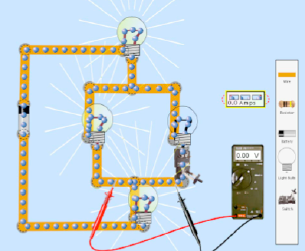
\includegraphics[width=6.4cm]{chapters/works/salehi-2.png}}
	\caption{Manipulativos usados por \cite{Salehi:2014}}
	\label{fig:salehi2014}
\end{figure}

O estudo foi feito com 32 estudantes universitários divididos em 16 pares, onde cada par trabalhou tanto com MF quanto com MV tendo que completar duas tarefas. Além disso, o experimento foi dividido em quatro blocos de acordo com a Tabela~\ref{tabela:salehi2014} e, em cada tarefa, os estudantes foram requisitados a mudar três vezes o valor de um dos resistores ($R_1$) e realizar medições de corrente e tensão dos diferentes componentes do circuito. Com esses dados, eles tiveram que elaborar teorias sobre a relação entre voltagem, corrente e resistência no circuito.
 
\begin{table}[htbp]
\caption{\textit{Design} experimental usado no estudo. Adaptado de~\cite{Salehi:2014}}
\centering
\begin{tabular}{|c|l|l|}
\hline
\textbf{Grupos} & \multicolumn{1}{c|}{\textbf{Tarefa 1}} & \multicolumn{1}{c|}{\textbf{Tarefa 2}} \\ \hline
\textbf{Bloco 1} & \begin{tabular}[c]{@{}l@{}}MV - Circuito em Série\\ 8 participantes\\ (4 pares)\end{tabular} & \begin{tabular}[c]{@{}l@{}}MF - Circuito em Paralelo\\ 8 participantes\\ (4 pares)\end{tabular} \\ \hline
\textbf{Bloco 2} & \begin{tabular}[c]{@{}l@{}}MV - Circuito em Paralelo\\ 8 participantes\\ (4 pares)\end{tabular} & \begin{tabular}[c]{@{}l@{}}MF - Circuito em Série\\ 8 participantes\\ (4 pares)\end{tabular} \\ \hline
\textbf{Bloco 3} & \begin{tabular}[c]{@{}l@{}}MF - Circuito em Série\\ 8 participantes\\ (4 pares)\end{tabular} & \begin{tabular}[c]{@{}l@{}}MV - Circuito em Paralelo\\ 8 participantes\\ (4 pares)\end{tabular} \\ \hline
\textbf{Bloco 4} & \begin{tabular}[c]{@{}l@{}}MF - Circuito em Paralelo\\ 8 participantes\\ (4 pares)\end{tabular} & \begin{tabular}[c]{@{}l@{}}MV - Circuito em Série\\ 8 participantes\\ (4 pares)\end{tabular} \\ \hline
\end{tabular}
\label{tabela:salehi2014}
\end{table}

Com relação a avaliação,~\cite{Salehi:2014} não detalham como foi calculada a pontuação ou o tipo de teste aplicado (questões abertas ou fechadas), mas afirma que para cada grupo foram executados três  testes conceituais (pré, meio e pós-teste), tendo sido calculadas as pontuações nos três testes, sendo que as pontuações dos testes do meio e pós-teste foram normalizadas a partir do pré-teste, sendo ``5'' a pontuação máxima para todos os três testes.

De modo geral, o estudo sugere que o uso de manipulativos físicos pode afetar positivamente o aprendizado e que a sequência das tarefas também pode afetar a nota final do estudante, onde os dados indicam que, para um maior ganho educacional, os manipulativos físicos deveriam ser utilizados antes dos manipulativos virtuais. Apesar disso, o artigo ainda afirma que a diferença entre iniciar com MF e prosseguir com MV ou o inverso não era estatisticamente significante, o que leva a entender que é possível inferir o mesmo que~\cite{zacharia:2011}, isto é, a ordem metodológica no uso de MF e MV não impacta substancialmente no aprendizado.

\begin{table}[htbp]
	\caption{Resumo - MF vs MV}
	\centering	
	\begin{tabular}{|l|c|c|c|c|c|c|c|c|}
		\hline
		\multicolumn{1}{|c|}{\textbf{Autor(es)}} & \textbf{MF} & \textbf{MV} & \textbf{MT} & \textbf{\begin{tabular}[c]{@{}c@{}}AE\end{tabular}} & \textbf{\begin{tabular}[c]{@{}c@{}}Coleta \\ dados\end{tabular}} & \textbf{\begin{tabular}[c]{@{}c@{}}AA\end{tabular}} & \textbf{\begin{tabular}[c]{@{}c@{}}Integração \\ com AVA\end{tabular}} & \textbf{\begin{tabular}[c]{@{}c@{}}Modelo \\ Genérico\end{tabular}} \\ \hline
		\begin{tabular}[c]{@{}l@{}}Zacharia e \\ Olympiou (2011)\end{tabular} & X & X &  & X &  &  &  &  \\ \hline
		Salehi et al. (2014) & X & X &  & X &  &  &  &  \\ \hline
	\end{tabular}
	\label{tabela:relatedsection1}
\end{table}

Assim como no trabalho de~\cite{zacharia:2011},~\cite{Salehi:2014} não coletam dados de interação dos alunos para Avaliação da Aprendizagem (AA) ou apresentam modos de calcular a aprendizagem. Além disso, embora ambos os trabalhos façam uma Avaliação Experimental (AE) e demostrem indícios de que o uso alternado de MF e MV melhorem a aprendizagem, não utilizam de manipulativos tangíveis (OT), o manipulativos utilizados não estão integrados a qualquer plataforma de aprendizagem e não apresentam um modelo genérico para a criação ou integração destes manipulativos, conforme apresentado na Tabela~\ref{tabela:relatedsection1}.

\subsection{Manipulativos Tangíveis (Físico-Digitais)}

\textbf{Melhorias nas habilidades espaciais}

\cite{ha:2018} propõem, implementam e avaliam o que chamam de ``Manipulativos Físico e Virtual ($MFV$)'' (do inglês, \textit{Virtual and Physical Manipulatives} - $VPM$), onde inserem um microcontrolador e sensores como acelerômetro, giroscópio e magnetômetro em manipulativos físicos com o objetivo de identificar as informações de orientação nos eixos x,y e z para rastrear os movimentos feitos pelos estudantes (Figura~\ref{fig:ha2018}). Além disso, cada manipulativo físico possui um correspondente ``virtual'' (Figura~\ref{fig:ha2018_VPM}) que é renderizado e movimentado de acordo com a manipulação física que o estudante executa, que o encaixa no conceito apresentado de objeto tangível.

\begin{figure}[htb]
	\centering
	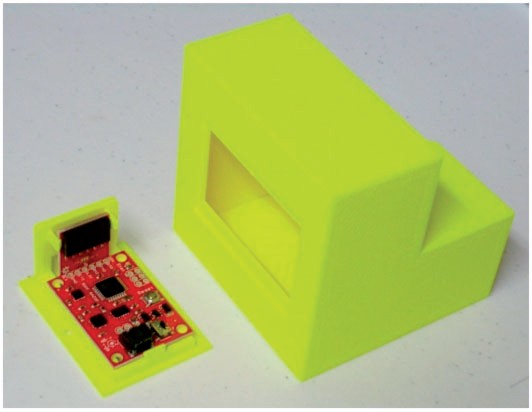
\includegraphics[width=0.7\linewidth]{chapters/works/ha2018.png}
	\caption{Manipulativo Físico com placa e sensores. Fonte:~\cite{ha:2018}}
	\label{fig:ha2018}
\end{figure}

Com o objetivo de treinar as habilidades espaciais na aula de matemática de estudantes da oitava série, especialmente no que diz respeito às habilidades de rotação mental de objetos, isto é, à capacidade de imaginar um objeto sendo rotacionado, ~\cite{ha:2018} projetaram dez tipos de $MFV$ com diferentes características geométricas de acordo com as especificações da Tabela~\ref{tab:ha2018}.

\begin{figure}[htb]
	\centering
	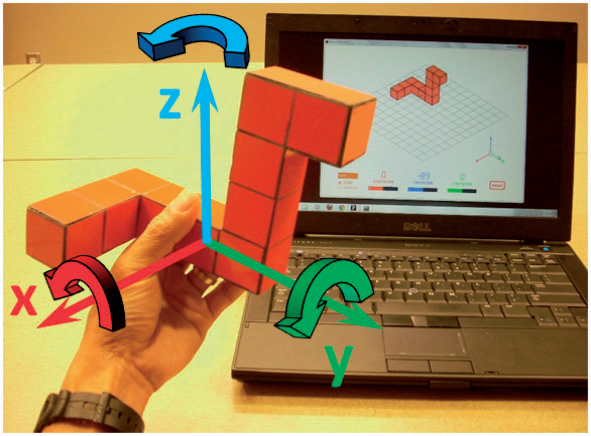
\includegraphics[width=0.7\linewidth]{chapters/works/ha2018_VPM.png}
	\caption{Manipulativo Físico e seu correspondente Virtual. Fonte:~\cite{ha:2018}}
	\label{fig:ha2018_VPM}
\end{figure}

Vale notar que os manipulativos físicos foram construídos através de impressoras 3D e os manipulativos virtuais foram projetados através do \textit{software} proprietário AutoCAD Inventor. Além disso, para avaliar os estudantes, foram realizados pré e pós-testes baseados no Teste de Visualização Espacial de Purdue (PSVT:R), que consiste em 30 questões de múltipla-escolha que ilustram um conjunto de figuras simétricas e não simétricas de objetos 3D em um formato isométrico 2D~\citep{ha:2018}.

\begin{table}[htbp]
\caption{Características Geométricas dos $MFV$ desenvolvidos por~\cite{ha:2018}}
\centering
\begin{tabular}{c|c|c|c|c|c|}
\cline{2-6}
\multicolumn{1}{l|}{} & \multicolumn{5}{c|}{\textbf{Características Geométricas}} \\ \hline
\multicolumn{1}{|c|}{\textbf{N.º}} & \textbf{\begin{tabular}[c]{@{}c@{}}Ângulo \\ Reto\end{tabular}} & \textbf{\begin{tabular}[c]{@{}c@{}}Superfícies \\ Cilíndricas\end{tabular}} & \textbf{\begin{tabular}[c]{@{}c@{}}Uma superfície \\ inclinada\end{tabular}} & \textbf{\begin{tabular}[c]{@{}c@{}}Múltiplas superfícies \\ inclinadas\end{tabular}} & \textbf{\begin{tabular}[c]{@{}c@{}}Múltiplas \\ Seções\end{tabular}} \\ \hline
\multicolumn{1}{|c|}{1} & X &  & X &  &  \\ \hline
\multicolumn{1}{|c|}{2} & X &  &  & X &  \\ \hline
\multicolumn{1}{|c|}{3} & X &  &  & X &  \\ \hline
\multicolumn{1}{|c|}{4} & X & X & X &  &  \\ \hline
\multicolumn{1}{|c|}{5} & X &  & X &  &  \\ \hline
\multicolumn{1}{|c|}{6} & X &  & X &  & X \\ \hline
\multicolumn{1}{|c|}{7} &  & X &  &  & X \\ \hline
\multicolumn{1}{|c|}{8} & X &  & X &  &  \\ \hline
\multicolumn{1}{|c|}{9} & X &  &  &  & X \\ \hline
\multicolumn{1}{|c|}{10} & X &  &  &  & X \\ \hline
\end{tabular}
\label{tab:ha2018}
\end{table}

Ao todo, sessenta e três alunos participaram das duas seções de experimento, entretanto, apenas os dados dos alunos que responderam as 30 questões foram utilizados, o que resultou em 44 alunos no pré-teste e 31 no pós-teste. A partir dos resultados de pré e pós-testes, foram calculados a pontuação de ganho e os ganhos de aprendizagem normalizados ($GAN$). As pontuações de ganho foram calculadas pela média da pontuação do pós-teste ($ps$) subtraída pela média do pré-teste ($pr$), enquanto o $GAN$ foi calculado de acordo com a Equação~\ref{equacao:hake1998}, proposta por~\cite{hake:1998}. Além disso, foram aplicados dois questionários, um de usabilidade com 21 itens baseados na Escala Likert e outro com uma questão Likert e outra aberta em que foi pedido que indicassem e justificassem a preferência por manipulativos (MF, MV ou ambos os tipos).

\begin{equation}\label{equacao:hake1998}
GAN = \frac{\% ps - \% pr}{100 - \% pr}
\end{equation}

De acordo com~\cite{ha:2018}, o uso de $MFV$ aumentou a pontuação média de todos os estudantes, onde a média no pré-teste foi 13,27(com desvio-padrão de 5,82) e a média no pós-teste foi 16,84 (com desvio-padrão de 7,58), com pontuação de ganho igual a 3,57 e ganho de aprendizagem normalizado igual a 21,3\%. O alto desvio padrão indica que as características de rotação mental é muito variável entre os estudantes analisados. Além disso, a análise estatística mostrou que a diferença entre os resultados do pré e do pós-teste é estatisticamente significativa. O mesmo aconteceu quando foram avaliados apenas os 21 estudantes que concluíram os dois testes.

Após apresentar estudos que indicam que pessoas do gênero masculino tendem a ter resultados melhores no que diz respeito a habilidades espaciais do que pessoas do gênero feminino, os dados do experimento mostram que o uso de MFV reduziu a diferença entre os gêneros de 21,5\% no pré-teste para 5,5\% no pós-teste.

Os resultados dos questionários de opinião mostram que 71,8\% dos estudantes consideram útil os MFV, 62,6\% consideram fácil de usar e, 81,3\% ficaram satisfeitos com o uso de MFV. Além do mais, a maioria dos estudantes (71,9\%) afirma preferir usar MFV do que o físico ou o virtual sozinhos porque os dois tipos de manipulativos compensam um ao outro além de alimentarem dois canais de aprendizagem (visual e tátil).

Embora, \cite{ha:2018} utilizem a expressão ``manipulativos físico e virtual'', é preciso salientar que o uso e a descrição correspondem ao que se propõe ser um manipulativo do tipo físico-digital e, portanto, objetos tangíveis de aprendizagem. Além disso, é importante notar que além de apresentar o uso de manipulativos tangíveis como uma ferramenta muito promissora para melhorar as habilidades espaciais dos estudantes, o objeto usado por \cite{ha:2018} apresentam evidências de que pode contribuir para a redução das desigualdades entre gêneros. 

Por fim, \cite{ha:2018} não oferecem elementos que garantam que o uso de manipulativos tangíveis melhorem a aprendizagem de maneira geral, não integram estes manipuláveis a uma plataforma com mecanismos de avaliação automática e/ou extraem dados de interação para análise de aprendizagem. Além disso, embora utilize questionários de múltipla-escolha, não fica claro como a pontuação dos alunos é calculada, o que permite supor que é utilizada a ``Pontuação Tradicional'' (Seção~\ref{sec:nota-tradicional}), isto é, levando em consideração unicamente se a resposta escolhida pelo aluno está certa ou errada.

\textbf{Disciplinas STEM}

\cite{Azad:2016} contextualizam seu trabalho em STEM, sigla em inglês que designa as seguintes áreas do conhecimento: Ciências, Tecnologia, Engenharia e Matemática, e em Internet das Coisas (IoT) apontando a importância do uso de sistemas ciberfísicos em uma abordagem educacional que seja interdisciplinar.

\begin{figure}[htb]
	\centering
	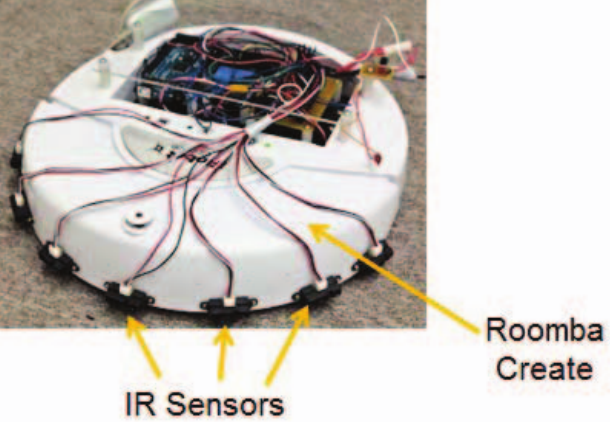
\includegraphics[width=0.6\linewidth]{chapters/works/azad2016.png}
	\captionsetup{justification=centering}
	\caption{RoCr com Arduíno e sensores infravermelho integrados. \\Fonte:~\cite{Azad:2016}}
	\label{fig:azad2016}
\end{figure}

Após uma introdução acerca da estrutura de sistemas ciberfísicos,~\cite{Azad:2016} apresentam três casos de estudo: (i) Casa Inteligente, com uso de Arduíno e sensores de luz e temperatura para controle automático de portas e de um equipamento de ventilação para ajuste da temperatura interna da casa, além de monitoramento remoto pelo usuário; (ii) \textit{Roomba Create} (RoCr), desenvolvido pela empresa \textit{iRobot}, que permite programar o comportamento do robô e que foi modificado para ser controlado remotamente pelo usuário ou funcionar de modo automático, tendo sido adicionados sensores de infravermelho e um Arduíno Mega (Figura~\ref{fig:azad2016}); e, (iii) sistemas embarcados de programação remota, que consiste em uma placa Arduíno com \textit{display} LCD, LEDs, motor de passos e um \textit{display} 7 segmentos com acesso remoto, conforme mostrado na Figura~\ref{fig:azad2016_remote}.

\begin{figure}[htb]
\center
\subfigure[ref1][Imagem da parte física]{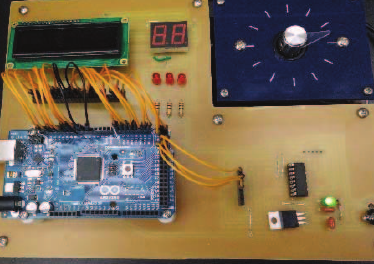
\includegraphics[width=7cm]{chapters/works/azad2016_remote1.png}}
\qquad
\subfigure[ref2][Imagem da GUI ]{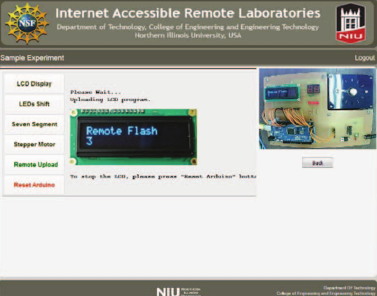
\includegraphics[width=6.4cm]{chapters/works/azad2016_remote2.png}}
\captionsetup{justification=centering}
\caption{Sistemas Embarcados de Programação Remota. \\Fonte:~\cite{Azad:2016}}
\label{fig:azad2016_remote}
\end{figure}

Com exceção do último caso, que utiliza Python no desenvolvimento, as propostas de~\cite{Azad:2016} utilizam a plataforma LabVIEW para implementação dos sistemas. Além disso, embora o trabalho seja contextualizado em STEM, os casos de uso apresentados não estão necessariamente aplicados no contexto educacional, além de não apontar elementos de coleta de dados, de integração a qualquer plataforma educacional ou de avaliação da aprendizagem.

\subsection{Modelagem Bifocal}

\cite{Blikstein:2012} e \cite{Blikstein2016} apresentam estudos que utilizam um \textit{framework} chamado Modelagem Bifocal (MB), onde manipulativos físicos e virtuais são justapostos. Segundo~\cite{Blikstein:2012}, no modelo bifocal, os estudantes constroem tanto um modelo físico, com sensores de um dado fenômeno científico, quanto um modelo virtual do mesmo fenômeno, conectando ambos em tempo real através de uma interface especial de \textit{hardware}, com o objetivo de compará-los.

De acordo com~\cite{Blikstein:2012}, a construção de um modelo bifocal implica que três tarefas principais sejam executadas pelos estudantes: (i) projetar um modelo físico para estudar o fenômeno científico usando sensores eletrônicos e a placa de baixo custo Gogo~\citep{sipitakiat:2003}; (ii) projetar um modelo virtual de computador do mesmo fenômeno usando um \textit{software} de modelagem, onde, normalmente, é usado o NetLogo, que é um ambiente de código-aberto e gratuito para modelagem baseada em agentes); e, (iii) conectar e executar ambos os modelos para compará-los e depurá-los.

\begin{figure}[htb]
	\centering
	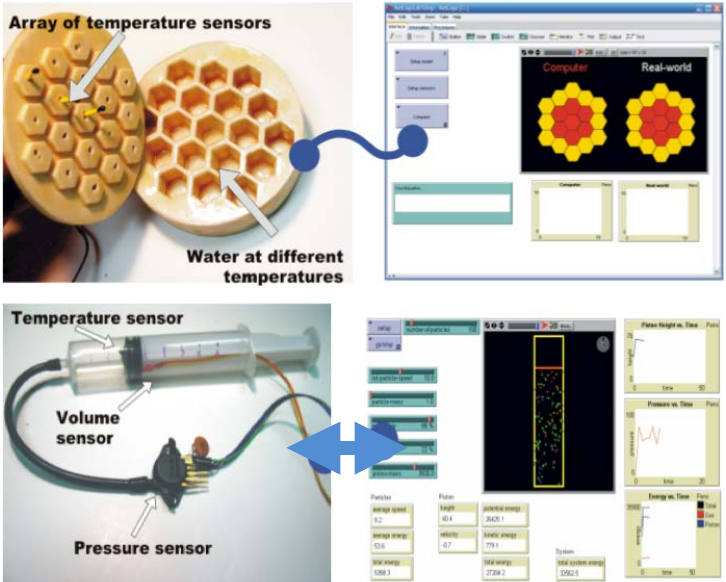
\includegraphics[width=0.8\linewidth]{chapters/works/blikstein2012.png}
	\captionsetup{justification=centering}
	\caption{Exemplos de Modelos Bifocais: transferência de calor e leis dos gases. Fonte:~\cite{Blikstein:2012}}
	\label{fig:blikstein2012}
\end{figure}

Desse modo,~\cite{Blikstein:2012} apresentam um prova de conceito com quatro estudos-piloto aplicando a MB na aprendizagem de fenômenos científicos em biologia, química e física em estudantes de ensino médio nos Estados Unidos. Os estudos consistiram em investigar e analisar padrão de crescimento de bactérias, leis de Newton a partir do tempo de uma bola descendo uma rampa, relação entre volume e pressão em um sistema fechado e difusão líquida. A Figura~\ref{fig:blikstein2012} apresenta dois exemplos de modelos bifocais propostos em~\cite{Blikstein:2012}, onde a esquerda podemos observar os manipulativos físicos e a direita os virtuais.

Além disso,~\cite{Blikstein:2012} dividiram as modelagens física e virtual em sequências de atividades menores que consistiram em: (i) pesquisa inicial para busca de fundamentos; (ii) projeto dos modelos com seleção de variáveis a ser observadas e construção de hipóteses a ser testadas; (iii) construção dos modelos físicos e virtuais para estudo do fenômeno; e, (iv) interação dos estudantes com os próprios modelos para observação, coleta de dados ou mudança de parâmetros. 

Com relação aos resultados, \cite{Blikstein:2012} apenas foca em como os estudantes resolveram as diferenças entre os modelos reais e virtuais, não apresentando estratégias de avaliação da aprendizagem ou se a abordagem de modelagem bifocal fez alguma diferença na aprendizagem das disciplinas propostas no estudo. Além disso, outra característica tanto de~\cite{Blikstein:2012} quanto de~\cite{Blikstein2016} é a metodologia baseada no trabalho de~\cite{Papert:1980} e~\cite{Papert:1994}.

\begin{table}[htbp]
	\caption{Resumo - Manipulativos Tangíveis}
	\centering
	\begin{tabular}{|l|c|c|c|c|c|c|c|c|}
		\hline
		\multicolumn{1}{|c|}{\textbf{Autor(es)}} & \textbf{MF} & \textbf{MV} & \textbf{MT} & \textbf{AE} & \textbf{\begin{tabular}[c]{@{}c@{}}Coleta\\ dados\end{tabular}} & \textbf{AA} & \textbf{\begin{tabular}[c]{@{}c@{}}Integração \\ com AVA\end{tabular}} & \textbf{\begin{tabular}[c]{@{}c@{}}Modelo\\ Genérico\end{tabular}} \\ \hline
		Ha Fang (2018) &  &  & X & X &  &  &  &  \\ \hline
		\begin{tabular}[c]{@{}l@{}}Azad e \\ Hashemian (2016)\end{tabular} &  &  & X &  &  &  &  &  \\ \hline
		\begin{tabular}[c]{@{}l@{}}Blikstein et \\ al. (2012) e (2016)\end{tabular} & X & X & X &  & X &  &  &  \\ \hline
	\end{tabular}
	\label{tabela:relatedsection2}
\end{table}

Por fim, a Tabela~\ref{tabela:relatedsection2} apresenta um resumo do apresentado nesta seção, de modo que é possível notar que, embora os trabalhos abordem a construção e o uso de manipulativos tangíveis, nenhum apresenta elementos para Avaliação da Aprendizagem (AA), Integração com Ambientes Virtuais de Aprendizagem (AVA) ou um modelo genérico para construção de objetos tangíveis compatíveis com alguma plataforma. Além disso, apenas uma abordagem proporciona coleta de dados, sendo que tal coleta não está relacionada a avaliação ou acompanhamento da aprendizagem através de dados provenientes da interação com os objetos de aprendizagem.

\subsection{Sistemas Físico-Virtuais de Aprendizagem no Brasil}

Nossa busca nas bases de dados da ``Comissão Especial de Informática na Educação'' (CEIE) da Sociedade Brasileira de Computação (SBC), que é a principal base brasileira de publicações na área de informática na educação, retornou apenas duas publicações evidentemente relacionadas a construção de ambientes baseados a sistemas ciberfísicos no contexto educacional no Brasil e que utilizam o termo ``físico-virtual'' ao invés de ``tangível''. Em contrapartida, uma grande quantidade de trabalhos recentes alinha-se ao desenvolvimento de ambientes tangíveis de aprendizagem.

\textbf{Plataforma Toogle}

\cite{Santos:2014} apresentam uma proposta embrionária de um ambiente físico-virtual de aprendizagem e uma plataforma para implementação de sistemas físico-virtuais, cuja arquitetura (Figura~\ref{fig:santos2014plataforma}) contém quatro módulos: (i) \textbf{\textit{Middleware} e Componentes:} proporciona comunicação entre as entidades físicas e virtuais do ambiente, sendo composto pelo \textit{framework} ROS (\textit{Robot Operating System}) que, por meio de ferramentas e bibliotecas próprias, fornece uma abstração de \textit{hardware}, \textit{drivers} para diversos dispositivos e um sistema de troca de mensagens; (ii) \textbf{Toogle Editor:} módulo que utiliza a ferramenta \textit{Blender} para adicionar, remover e editar componentes físico-virtuais, além dos objetivos do ambiente; (iii) \textbf{Inteligência de Ambiente:} fornece um conjunto ordenado de recursos para conduzir o ambiente ao alcance dos objetivos estabelecidos; e, (iv) \textbf{Toogle Navegador:} possibilita a interação dos usuários com o ambiente, provendo por exemplo, informações sonoras, estereoscópicas, táteis, dentre outras, além de um \textit{plugin} para Web. 
Além disso, o trabalho publicado por~\cite{Santos:2014} é derivado da tese de doutorado do mesmo autor principal, isto é~\cite{santos:2014ambientes}, igualmente defendida em 2014. 

\begin{figure}[htb]
	\centering
	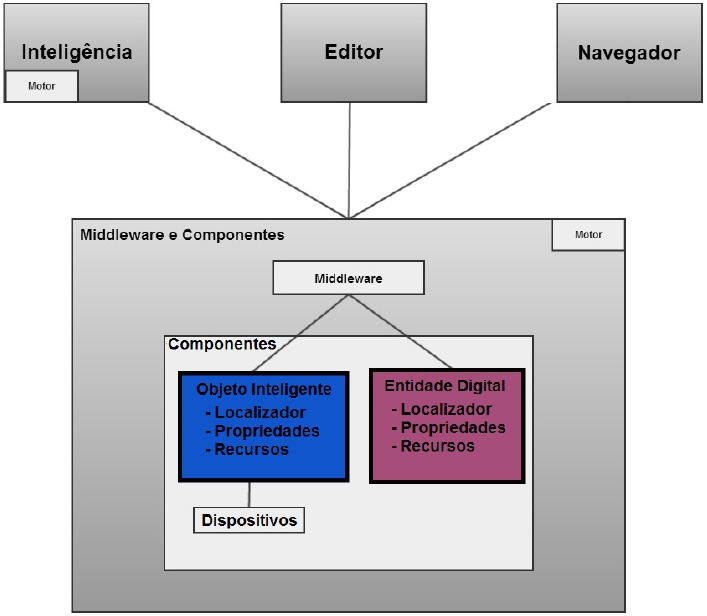
\includegraphics[width=0.8\linewidth]{chapters/works/santos2014_arquitetura.png}
	\caption{Arquitetura da Plataforma Toogle. Fonte:~\cite{Santos:2014}}
	\label{fig:santos2014plataforma}
\end{figure}

Após apresentar a plataforma Toogle e baseando-se no trabalho de~\cite{xu:2005}, que apresenta um modelo conceitual para um ambiente virtual de aprendizagem construtivista, ~\cite{Santos:2014} e~\cite{santos:2014ambientes} propõem um modelo conceitual para ambientes físico-virtuais de aprendizagem (Figura~\ref{fig:santos2014modelo}), o qual está relacionado com a plataforma apresentada. Tal modelo contém os sete elementos a seguir: (i) \textbf{aluno e contexto:} ``alunos'' são identificados como atores que interagem com o ambiente com o objetivo de aprender, enquanto o ``contexto'' pode ajudar nos momentos de aprendizagem, por exemplo, estabelecendo novos conteúdos; (ii) \textbf{professores: } elaboram os currículos, determinam os objetivos de aprendizagem e mediam as adaptações (oportunismo) das situações de aprendizagem; (iii) \textbf{situação: } formaliza o contexto da situações de aprendizagem usando a abordagem de solução de problemas \textit{STRIPS}, proposta por~\cite{fikes:1971}, além de oferecer novas oportunidades para o ensino; (iv) \textbf{oportunismo: }sugerir situações de aprendizagem (com elementos físicos e virtuais) baseando-se nas interações prévias ou atuais dos estudantes; (v) \textbf{interação: }proporciona espaços de interação em que há a mistura de elementos físicos e virtuais; (vi) \textbf{objetivos de aprendizagem: } indicados pelo professor, são o enfoque das atividades; (vii) \textbf{currículo:} armazena as informações do currículo, além de possibilitar que o professor desenvolva objetos de aprendizagem que sejam físico-virtuais.

\begin{figure}[htb]
	\centering
	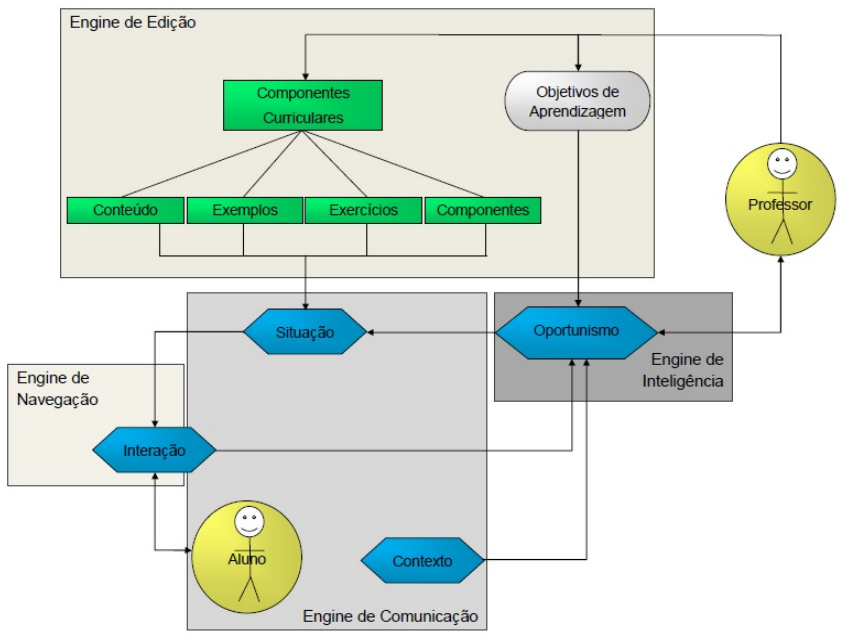
\includegraphics[width=0.9\linewidth]{chapters/works/santos2014_modelo_v2.png}
	\captionsetup{justification=centering}
	\caption{Modelo Conceitual de um Ambiente Físico-Virtual de Aprendizagem proposto por~\cite{santos:2014ambientes}}
	\label{fig:santos2014modelo}
\end{figure}

O estudo de caso de~\cite{Santos:2014} foi a criação de uma aula com os seguintes componentes: sala de aula, aluno, professor, apostila 1, apostila 2 e \textit{smartphone}. Desse modo, foi introduzido um modelo em 3D de um prédio com várias salas de aula às quais foram associadas coordenadas de GPS que serviriam de gatilho para a visualização de apostilas em PDF, sendo a visualização das mesmas o objetivo de aprendizagem definido pelo professor. Além disso, o componente \textit{smartphone} estaria associado a um componente ``prevê\_posição'' para que as posições do aluno fossem coletadas e, então, se verificasse se a posição atual coincide com a posição do objetivo de aprendizagem.

A comunicação entre os diversos módulos da plataforma acontece através de arquivos XML que, por último, são enviados ao módulo de ``inteligência do ambiente'' que planeja a execução dos recursos. O artigo não detalha o modo como esse planejamento acontece, embora mencione que a execução das ações acontece mediante verificação das propriedades dos recursos, por exemplo, enquanto a apostila não tiver sido visualizada, o sistema pode enviá-la assim que determinado estudante atingir a localização geográfica associada a ela.

\cite{Santos:2014} concentra-se somente em definir uma arquitetura geral de como deveria ser um ambiente físico-virtual de aprendizagem e em implementar um exemplo dessa arquitetura, sem desenvolver/aplicar ferramentas/estratégias de gerência ou avaliação da aprendizagem e sem explorar dados relacionados a interação dos alunos com o material didático. Além disso, a plataforma e o modelo apresentados cobrem efetivamente apenas quatro dos oito requisitos requisitos de um ambiente físico-virtual de aprendizagem definidos por~\cite{santos:2014ambientes}.

\textbf{Leitura colaborativa em ambiente físico-virtual}

O trabalho de~\cite{imamura:2018} segue uma linha de leitura colaborativa que toma por base o construtivismo e o enativismo, onde, de acordo com os autores, no primeiro caso, o conhecimento é tido como algo a ser construído a partir das relações físicas e sociais estabelecidas pelos indivíduos e, no segundo, o conhecimento está relacionado a uma descoberta pela ação, a uma sensorialidade ou a uma experimentação do mundo físico~\citep{imamura:2018}. 

Assim, a pesquisa de~\cite{imamura:2018} utiliza realidade aumentada para viabilizar a implementação de um sistema socioenativo de Leitura Colaborativa Físico-Virtual (LCFV) que leva em consideração a exploração física do espaço por meio de uma aplicação para \textit{smartphones}, conforme mostrado na Figura~\ref{fig:imamura2018}.

O primeiro protótipo do projeto utilizou \textit{QR Codes} em cada objeto físico para dar acesso a sua representação e conteúdo virtuais e para o cenário de leitura foi criada uma narrativa baseada em um desafio onde o objetivo dos participantes era descobrir o que aconteceu usando informações do ambiente físico-virtual. Embora o primeiro experimento tenha sido feito com quatro estudantes de pós-graduação, o desafio foi proposto para ser aplicado a crianças de 10 anos que visitassem o Museu Exploratório de Ciências da Unicamp.

\begin{figure}[htb]
	\centering
	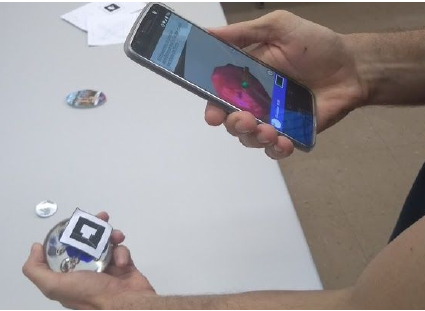
\includegraphics[width=0.6\linewidth]{chapters/works/imamura2018.png}
	\captionsetup{justification=centering}
	\caption{Exemplo de exploração do cenário físico usando \textit{smartphone}. Fonte:~\cite{imamura:2018}}
	\label{fig:imamura2018}
\end{figure}

\cite{imamura:2018} indicam que o primeiro protótipo para LCFV foi implementado de modo que cada grupo tivesse 4 leitores e um moderador que conhece o funcionamento da história, tendo sido utilizados 14 objetos físicos com \textit{QR Code} e 5 objetos sem interações virtuais diretas. Além disso, cada leitor recebe um papel diferente (cientista, programador, atleta e professor), onde cada um terá acesso a diferentes informações do objeto físico durante dois minutos. Assim, há um rodízio que faz com que, enquanto um membro do grupo ``explora'' o cenário, os outros levantam questionamentos e hipóteses que ajudem a compor a narrativa (Figura~\ref{fig:imamura2018_LCFV}).

\begin{figure}[htb]
	\centering
	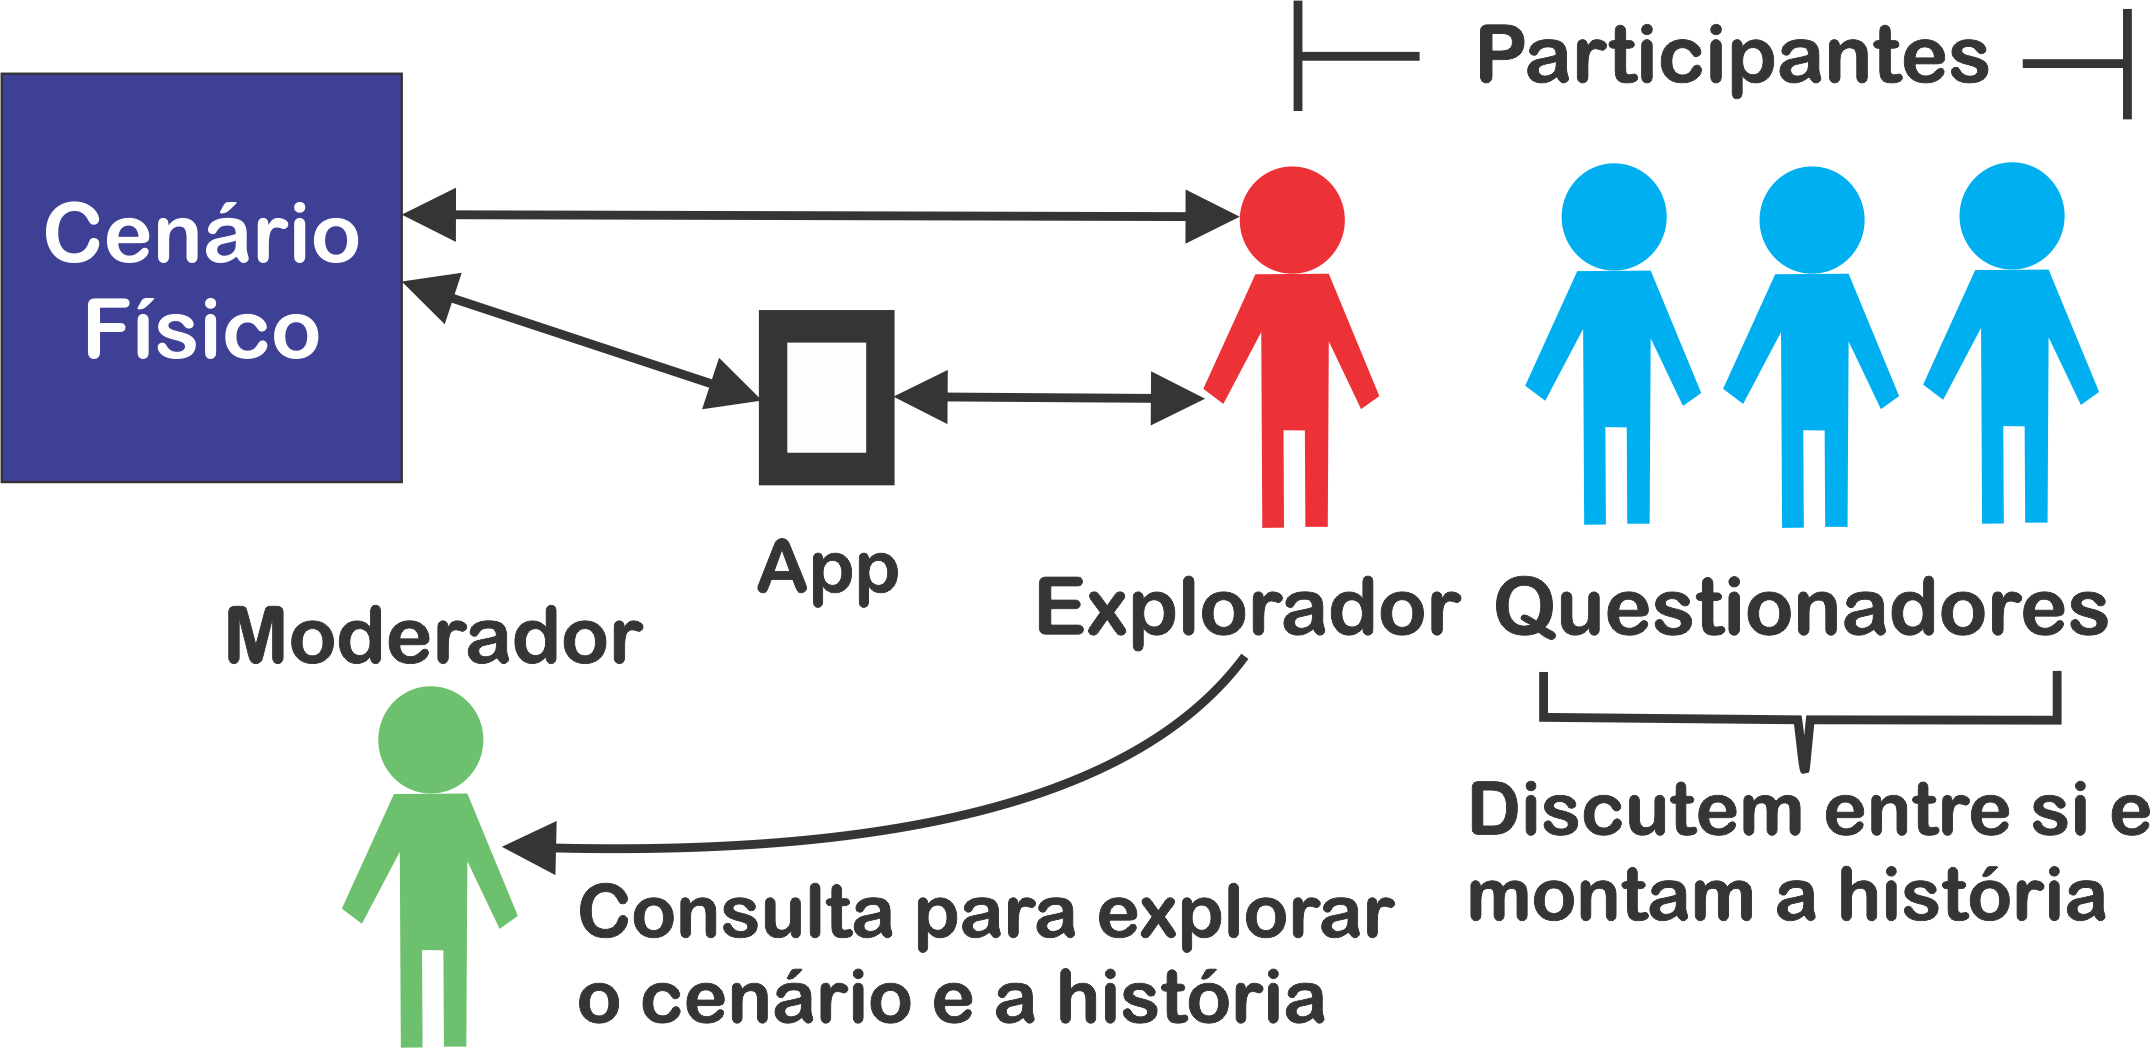
\includegraphics[width=0.7\linewidth]{chapters/works/imamura2018_LCFV.png}
	\captionsetup{justification=centering}	
	\caption{Configuração da LCFV para o primeiro experimento. \\Fonte:~\cite{imamura:2018}}
	\label{fig:imamura2018_LCFV}
\end{figure}

Segundo~\cite{imamura:2018}, a leitura colaborativa deve resultar em ``um texto estruturado por imagens, colagens, diagramas e falas dos participantes''. Além disso, os participantes também tem disponíveis objetos que ajudem a organizar as informações, tais como materiais de escrita, \textit{post-it} e um espaço para colocar as perguntas envolvendo a história, reflexões resultantes da experiência, conexões feitas entre o que foi explorado e o mundo exterior.

Após a atividade, foi feita uma avaliação utilizando um questionário AttrakDiff que, de acordo com~\cite{imamura:2018}, usa uma escala semântica de -3 a 3 para avaliar aspectos da experiência do usuário tais como atratividade, estímulo e qualidade pragmática e hedônica. Assim, de acordo com essa avaliação, a experiência dos usuários foi expressa através de palavras com 100\% de concordância dos participantes (`agradável',`convidativo', `criativo', `cativante' e `motivadora'), com concordância acima de 80\% (`prática', `integradora', `boa', `inovadora', `desafiadora', `nova', `profissional', `imprevisível' e `apresentável'). Além disso, houve menos concordância a respeito se a experiência foi `confusa' ou `claramente estruturada'.

Embora proponha algo muito inovador, não somente pela inserção de sistemas ciberfísicos, mas também pela proposta de leitura colaborativa com uma abordagem socioenativa, o trabalho de~\cite{imamura:2018}
não prevê um modo de avaliar automaticamente a aprendizagem dos estudantes (especialmente por que o cenário demanda algum nível de imprevisibilidade) e não utiliza os elementos tangíveis em associação a uma plataforma educacional mais ampla.

\textbf{Objetos Tangíveis no Ensino de Matemática}

\cite{lima:2016} apresentam uma proposta de design colaborativo de objetos tangíveis para crianças e uma versão tangível do Tangram que fornece \textit{feedback} automático aos estudantes e professores com relação a posição das peças (se foram colocadas corretamente ou não). De acordo com os autores, o jogo Tangram possibilita o aprendizado de conceitos geométricos de frações, lados, ângulos, formatos semelhantes, perímetro e área de figuras planas, semelhanças de triângulos, ângulos e polígonos congruentes.

\begin{figure}[htb]
	\centering
	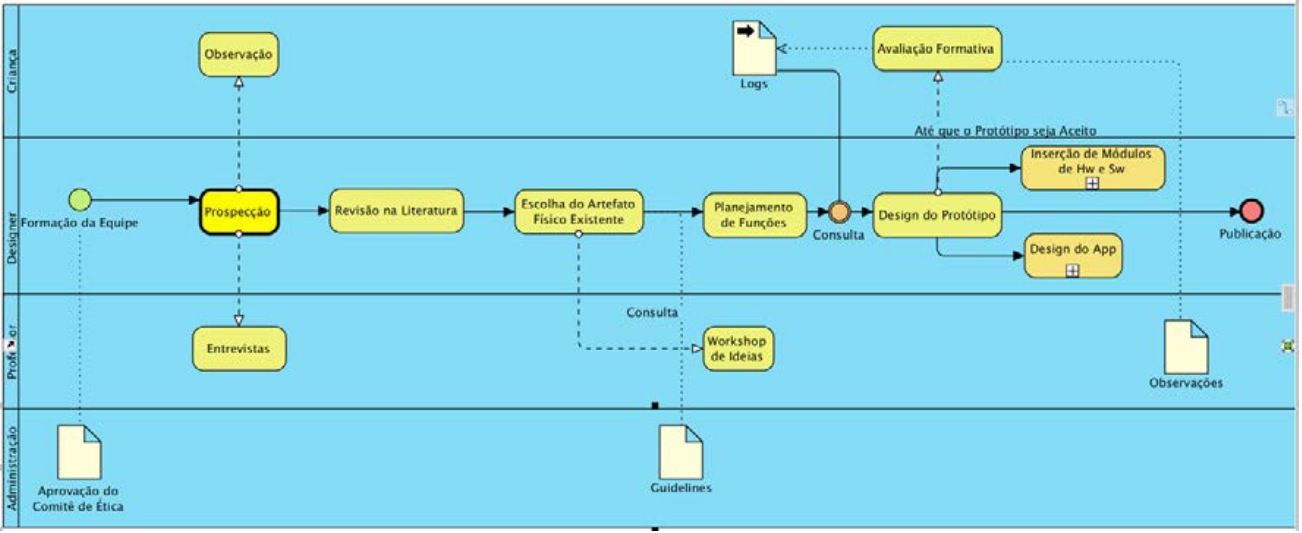
\includegraphics[width=1\linewidth]{chapters/works/lima2016.png}
	\captionsetup{justification=centering}	
	\caption{Processo de Design em Artefatos Tangíveis para Crianças. \\Fonte:~\cite{lima:2016}}
	\label{fig:lima2016}
\end{figure}

Como parte da metodologia utilizada, uma abordagem baseada em Design Participativo foi adaptada de modo que o objeto tangível fosse gerado a partir da observação e colaboração de crianças que utilizariam o jogo, além disso é apresentada uma descrição do modelo de processo utilizando diagrama BPMN (Figura~\ref{fig:lima2016}).

\begin{figure}[htb]
	\center
	\subfigure[ref1][Peça com sensores e Arduíno embutidos ]{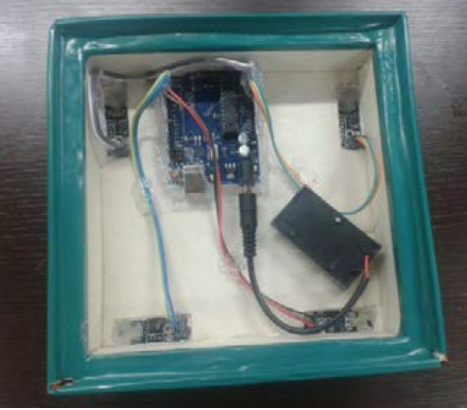
\includegraphics[width=7cm]{chapters/works/lima2016-2.png}}
	\qquad
	\subfigure[ref2][Peças do Tangram instrumentadas com sensores ]{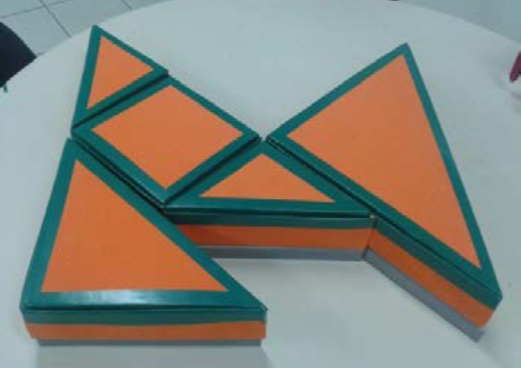
\includegraphics[width=6.4cm]{chapters/works/lima2016-3.png}}
	\captionsetup{justification=centering}
	\caption{Protótipo do Tangram Tangível}
	\label{fig:lima2016_prototipo}
\end{figure}

Foram elaborados dois protótipos funcionais, onde o primeiro protótipo foi apenas uma prévia para o segundo, de modo que os  materiais utilizados na construção das sete peças do Tangram no protótipo final (Figura~\ref{fig:lima2016_prototipo}) foram: ``Arduíno Uno, Sensor \textit{Hall}, \textit{Shield Bluetooth}, \textit{Jumper wires}, Cabo USB, LED, Tecido inteligente, Cartolina, Emborrachado, Papelão Branco, Régua, Lápis, Pincel e Fitas''. 
Como parte da proposta do jogo, foi implementado um aplicativo Android (Figura~\ref{fig:lima2016_app}) com imagens que deveriam ser selecionadas pelos estudantes e replicadas utilizando o objeto tangível.

\begin{figure}[htb]
	\centering
	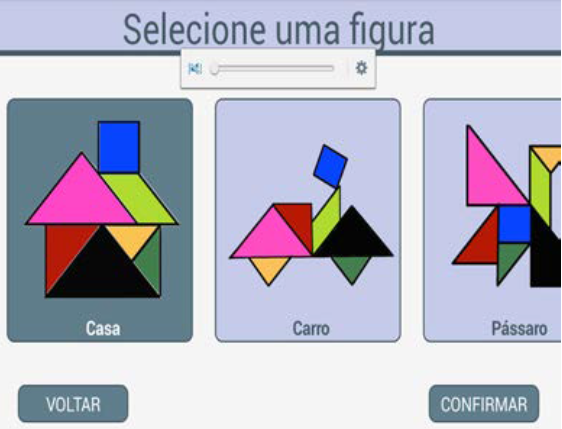
\includegraphics[width=0.6\linewidth]{chapters/works/lima2016-4.png}
	\caption{Tela do App para o Tangram Tangível. \\Fonte:~\cite{lima:2016}}
	\label{fig:lima2016_app}
\end{figure}

Por fim, é importante salientar que, embora o trabalho comente sobre o fornecimento de um \textit{feedback} para estudantes e professores e sobre uma avaliação formativa ter sido realizada, não são apresentados mais detalhes além de que essa avaliação fez parte do processo de construção dos protótipos. Além disso, o trabalho não prevê um método de avaliação da aprendizagem usando dados coletados pelo objeto tangível, bem como o protótipo não está integrado a qualquer ambiente de aprendizagem mais abrangente.

\textbf{Ambiente Virtual Tangível no Ensino de Ciências}

\begin{figure}[htb]
	\centering
	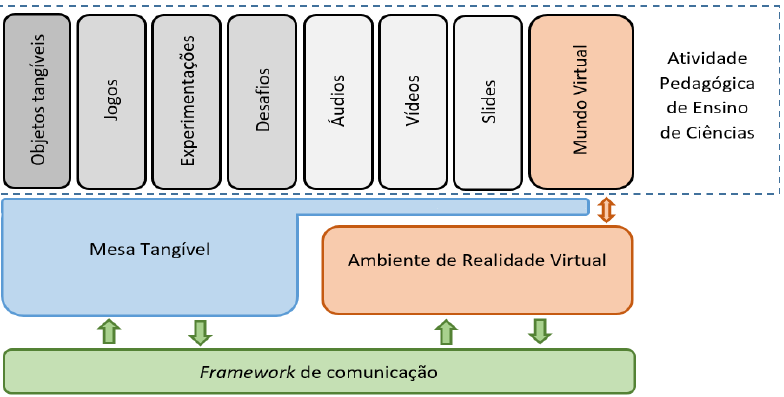
\includegraphics[width=0.8\linewidth]{chapters/works/gluz2018.png}
	\captionsetup{justification=centering}
	\caption{Integração da MT e RV numa atividade pedagógica. \\Fonte:~\cite{gluz:2018}}
	\label{fig:gluz2018-framework}
\end{figure}

\cite{gluz:2018} apresentam uma proposta de ambiente de aprendizagem que utiliza objetos tangíveis e realidade virtual 3D, que denominam de ``Ambiente de ensino Virtual Tangível (AVT)'', cujo objetivo é auxiliar no ensino de Ciências numa perspectiva inclusiva, com estudantes que tem déficit de comunicação.

Como objeto tangível é utilizada uma Mesa Tangível (MT), que provê uma superfície onde os estudantes podem manipular os objetos de modo que essa manipulação física seja comunicada a um ambiente de Realidade Virtual (RV) 3D através de um \textit{framework} especialmente construído para isso. A Figura~\ref{fig:gluz2018-framework} apresenta como as partes desse ambiente se comunicam.

De acordo com \cite{gluz:2018}, a construção da MT contou com os seguintes materiais: estrutura de madeira, superfície de acrílico e vinil translúcido, LEDs de infravermelho, projetor, câmera de infravermelho e um computador. O software da MT é composto de um editor, um player e uma biblioteca de protocolos de comunicação, tendo sido desenvolvido utilizando tecnologias web como HTML5 e JavaScript. Além disso, a comunicação com a RV é feita através de \textit{web services}.

\begin{figure}[htb]
	\centering
	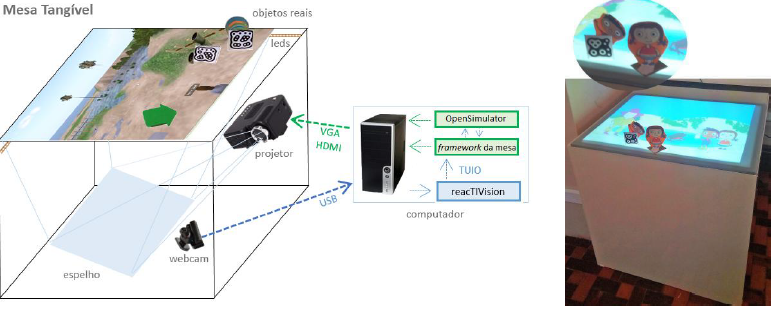
\includegraphics[width=0.9\linewidth]{chapters/works/gluz2018-mesa.png}
	\caption{Estrutura e componentes da mesa tangível. \\Fonte:~\cite{gluz:2018}}
	\label{fig:gluz2018-mesa}
\end{figure}

A Figura~\ref{fig:gluz2018-mesa} apresenta o esquema dos componentes da mesa tangível e uma imagem da mesa real construída, onde se pode observar a superfície tangível através da qual os estudantes interagem com o ambiente virtual utilizando objetos físicos. 

No contexto da proposta apresentada por \cite{gluz:2018}, o AVT apresenta uma história educativa ambientada no Parque Estadual de Itapeva (RS) contendo quatro personagens com diferentes funções dentro da história e que interagem com os estudantes como um agente pedagógico inteligente cujo objetivo é explicar, guiar, interagir e lançar desafios aos estudantes.

Ademais, o trabalho apresentado é centrado na descrição do desenvolvimento do ambiente virtual e da prova de conceito, inclusive apresentando a proposta de roteiro da história implementada, de modo que os próprios autores comentam que o próximo seria a realização de experimentos empíricos em sala de aula. Assim, o ambiente virtual tangível, sendo uma proposta ambiente educacional, possibilita o uso de diferentes objetos de aprendizagem (objetos tangíveis, jogos, desafios, áudios, vídeos, slides,...), mas, não pressupõe alguma abordagem de avaliação da aprendizagem ou coleta de dados de interação dos estudantes com a mesa tangível.


Por fim, a Tabela~\ref{tabela:relatedsection_br} apresenta um resumo dos trabalhos desta seção, de modo a melhor comparar as suas características. Assim, nenhum dos trabalhos apresenta isoladamente um objeto físico ou virtual, mas, objetos que podem ser considerados tangíveis, uma vez que tais objetos contém elementos físicos e virtuais que, de algum modo, estão integrados entre si. Apenas dois trabalhos fazem uma Avaliação Experimental (AE) \citep{imamura:2018,lima:2016}, dois trabalhos tem algum tipo de integração com um ambiente de aprendizagem \citep{santos:2014ambientes, gluz:2018}, embora \cite{santos:2014ambientes} apresente um modelo e uma instância de um ambiente `físico-virtual' que provê objetos tradicionais e, outros dois trabalhos \citep{santos:2014ambientes,lima:2016} apresentam modelos genéricos relacionados a objetos físico-virtuais (tangíveis). É importante notar que nenhum dos trabalhos apresenta coleta de dados e nem avaliação da aprendizagem, inclusive através de dados provenientes destas coletas.

\begin{table}[htbp]
	\caption{Resumo - Sistemas Físico-Virtuais no Brasil}
	\centering
	\begin{tabular}{|l|c|c|c|c|c|c|c|c|}
		\hline
		\multicolumn{1}{|c|}{\textbf{Autor(es)}} &
		\textbf{MF} &
		\textbf{MV} &
		\textbf{MT} &
		\textbf{AE} &
		\textbf{\begin{tabular}[c]{@{}c@{}}Coleta\\ dados\end{tabular}} &
		\textbf{AA} &
		\textbf{\begin{tabular}[c]{@{}c@{}}Integração \\ com AVA\end{tabular}} &
		\textbf{\begin{tabular}[c]{@{}c@{}}Modelo\\ Genérico\end{tabular}} \\ \hline
		Santos et al. (2014)                                                    &  &  &   &   &  &  & X & X \\ \hline
		\begin{tabular}[c]{@{}l@{}}Imamura e \\ Baranauskas (2018)\end{tabular} &  &  & X & X &  &  &   &   \\ \hline
		Lima et al. (2016)                                                      &  &  & X & X &  &  &   & X \\ \hline
		Gluz et al. (2018)                                                      &  &  & X &   &  &  & X &   \\ \hline
	\end{tabular}
	\label{tabela:relatedsection_br}
\end{table}

% \section{Ambientes de Aprendizagem} 
% \label{section:LearninAmbients}

% \cite{Garcia:2010} afirma que há dois tipos de aprendizado: o formal, que ocorre dentro da sala de aula, e o informal, que acontece fora dela. O primeiro tipo é mais comum na educação escolar tradicional, entretanto, o segundo tipo inclui todos os lugares que não sejam, à primeira vista, um ambiente de sala de aula em si. Nessa perspectiva, a casa do estudante, um museu, um parque, ou qualquer outro local pode ser considerado ambiente de aprendizagem, visto que está passível de ocorrer nele uma situação de aprendizado informal. Considerando esses fatores, classificaremos os ambientes de sala de aula inteligente em dois tipos:

% \begin{enumerate}
% 	\item \textbf{Ambiente interno:} são aqueles desenvolvidos num contexto de salas de aula formal. Trabalhos relacionados ao ensino à distância, ao uso de dispositivos móveis, sensores ou computadores vestíveis que necessitem da presença dos estudantes e do professor simultaneamente e que simule uma sala de aula formal também estão contidos nesta classificação. 
	
% 	\item \textbf{Ambiente externo:} contextos educacionais ao ar livre o que implica em ambientes mais abertos como museus, zoológicos, parques, ou até mesmo a casa do estudante. Trabalhos relacionados ao ensino à distância, ao uso de dispositivos móveis, sensores ou computadores vestíveis que permitam mobilidade e liberdade dos estudantes em relação ao conteúdo e tempo de estudo também se encaixam nessa classificação.
% \end{enumerate}

% % -----------------------------------------------------------------
% => Ambiente Interno
% -----------------------------------------------------------------

\subsection{Ambiente Interno de Aprendizagem}
\label{section:wIndoorClassroom}

%Abordagens de construção de ambientes ou componentes de sala de aula presencial tem sido objeto de estudo de alguns trabalhos, em geral, esses trabalhos enfocam o uso de RFID (\textit{Radio-Frequency IDentification}), câmeras, servidores, novos tipos de mobiliário, lousas inteligentes e dispositivos móveis.

\cite{Bargaoui:2014} apresentam um \textit{Gateway} para conectar os múltiplos dispositivos utilizados numa sala de aula inteligente. Para construção da solução são utilizados RFID, servidor de dados, ferramentas de administração, lousa inteligente, \textit{Raspberry-Pi}, OSGi (\textit{Open Service Gateway Initiative}) e dispositivos inteligentes diversos. Como trabalhos futuros, é sugerida a criação de um modelo de avaliação da experiência do estudante e compará-lo com uma sala de aula clássica.

\cite{Margetis:2011} descrevem uma abordagem a partir da aplicação de Inteligência de Ambientes em sala de aula e faz um levantamento de requisitos importantes a serem levados em consideração a fim de ajudar de modo mais eficiente na melhoria da educação dos estudantes. Utiliza um \textit{framework} chamado ClassMATE (\textit{Classroom Multiplatform Augmented Technology Environment}) dentre outras ferramentas como: FAMINE (\textit{FORTH's AMI Network Environment}), PERSONAF (\textit{Personalised Pervasive Scrutable Ontological Framework}), \textit{Learning Technology Systems Architecture} (LTSA), Desk aumentado, lousa inteligente, PUPIL (um \textit{front-end educacional}) que são aplicações eletrônicas para sala de aula (Figura~\ref{fig:margetis2011}).

\begin{figure}[ht]
\centering
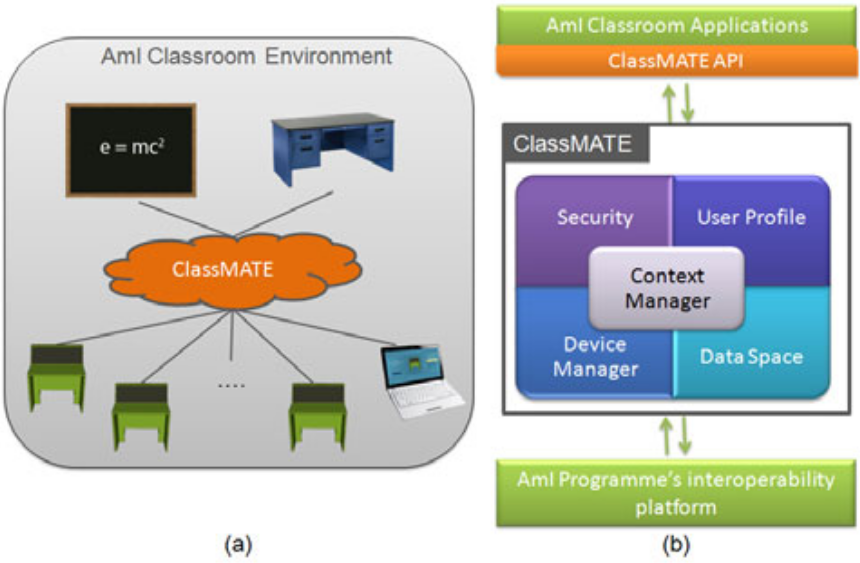
\includegraphics[width=0.8\linewidth]{imgs/margetis2011}
\caption{(a) Cenário do ClassMATE. (b) Arquitetura do ClassMATE}
\label{fig:margetis2011}
\end{figure}

\cite{Chang:2014} apresentam soluções de transformação de salas de aula tradicionais em salas de aula inteligentes baseadas em Internet das Coisas (IoT). Apresentam a definição de uma estrutura IoT composta por quatro camadas: \textit{Perceptive Layer, Network Layer, Processing Layer, Application Layer}. Afirma que há uma relação entre essas camadas e uma sala de aula. Assim, para tornar uma escola tradicional uma escola inteligente é necessário atingir três pontos:

\begin{enumerate}
   \item "Transformar uma sala de aula tradicional em uma IoT-base" através da instalação de um Set-top-box (STB) com webcam, RFID, Wifi e outras ferramentas de transmissão de dados (Figura~\ref{fig:chang2014}).
   \item Analisar o comportamento de aprendizagem dos alunos usando o RFID instalado no STB para identificar individualmente a presença do aluno na sala, além de enviar informações das respostas dos exercícios no \textit{tablet} ou \textit{smartphone} para gerar estatísticas relativas ao desempenho e às dificuldades dos alunos em determinado conteúdo de uma disciplina;
   \item Gerenciar dispositivos inteligentemente usando \textit{tablet} se comunicando através de Zigbee\footnote{Tecnologia de comunicação sem fio desenvolvida pela \textit{Zigbee Alliance} como padrão global aberto visando baixos custo e consumo de energia~\citep{Digi:2017}} para controlar dispositivos como projetor, ventilador, ar-condicionado e luzes.
\end{enumerate}

Ao detalhar os componentes de cada um desses pontos, o artigo apresenta em qual camada IoT um componente específico está localizado.

\begin{figure}[ht]
	\centering
	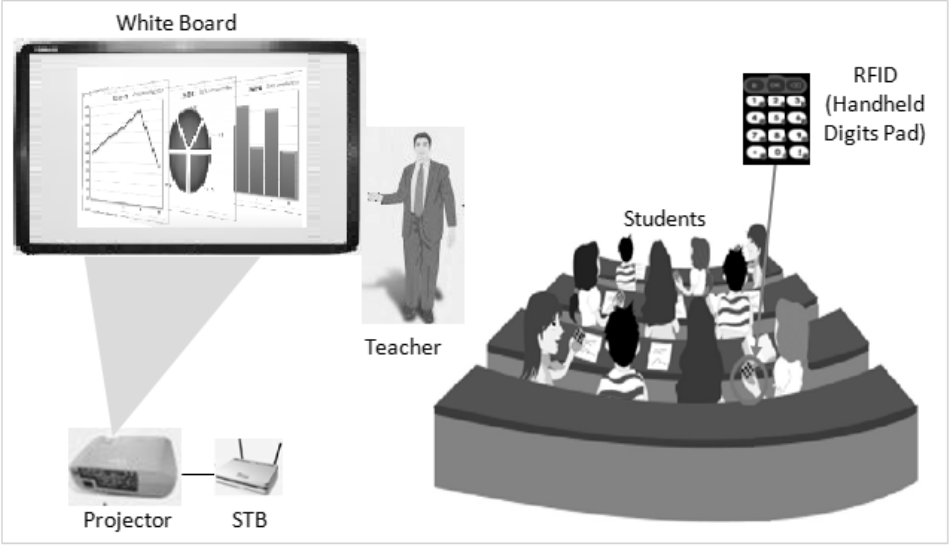
\includegraphics[width=0.8\linewidth]{imgs/Chang2014}
	\caption{Cenário de Sala de Aula Inteligente}
	\label{fig:chang2014}
\end{figure}

\cite{Savvaki:2013} apresentam o projeto de uma nova mesa (desk) para estudantes em uma sala de aula inteligente. A nova configuração utiliza como requisitos de projeto elementos de Estética, Usabilidade, Tecnologia e Viabilidade. Inicialmente, foram projetadas quatro alternativas baseadas no uso de tablet, mas, a versão final propõe um computador \textit{all-in-one} embarcado em uma estrutura que também permite atividades baseadas em papel (Figura~\ref{fig:Savvaki2013}). Duas mesas adjacentes podem se conectar e possibilitar atividades colaborativas e, assim, promover trabalhos em equipe.

\begin{figure}[ht]
\centering
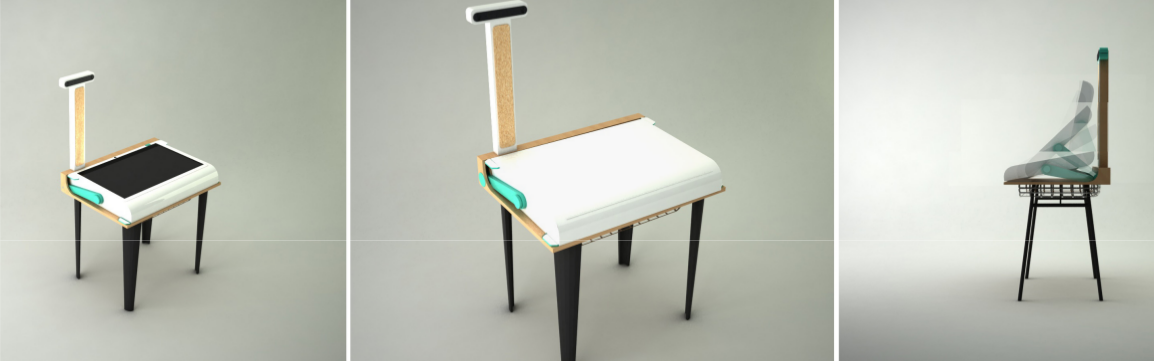
\includegraphics[width=0.9\linewidth]{imgs/Savvaki2013}
\caption{Mesa de estudos inteligente}
\label{fig:Savvaki2013}
\end{figure}

O trabalho de \cite{Zhang:2003} foca em aprendizado remoto que utiliza: protocolo multicast híbrido aplicação-camada, um software dedicado chamado "\textit{SameView}", uma sala de aula inteligente que é uma sala de aula ampliada com telas do tamanho da parede, sensores, câmeras e módulos de percepção e computação associados, alguns tipos de tecnologia de computação de padrões de aprendizagem, aprendizagem de interconexão através de protocolos de comunicação com e sem fio. A ideia é proporcionar maior participação na aula para quem está assistindo remotamente.

\cite{Mathioudakis:2013} apresentam uma abordagem centrada no aluno para dar apoio aos professores na melhoria do processo de aprendizado em ambientes educacionais. O sistema proposto apresenta uma infraestrutura multiagente inteligente que monitora, discretamente, as atividades dos alunos e notifica o professor, em tempo real, sobre as potenciais deficiências e armadilhas que precisam ser tratadas. O trabalho também aborda a questão da identificação do comportamento e análise de estatística de sala de aula.

O trabalho de \cite{Hwang:2009} está contextualizado no ensino da prática de laboratório de Difracção de Raios X de cristal único para pesquisadores inexperientes. O sistema identifica em que parte do laboratório o estudante está e, assim, infere a atividade que será executada por ele. Associando essa informação de contexto à temperatura ambiente, o estudante recebe instruções dos procedimentos que devem ser feitos, por exemplo, a seleção de um cristal de qualidade e tamanho adequado para a atividade a ser feita. Essas instruções são passadas através de um PDA (\textit{Personal Digital Assistant}). A efetividade do sistema foi medida através de pesquisa de opinião com os próprios estudantes que relataram uma melhoria no desempenho e na praticidade das aulas de laboratório.

Para \cite{Santana:2013}, simplesmente utilizar dispositivos móveis em sala de aula não é suficiente, é necessário que esses dispositivos se comuniquem entre si e contribuam com a melhoria do processo de ensino-aprendizagem. Este trabalho descreve a aplicação do conceito de Inteligência de Ambientes para criação de um ambiente educacional adaptado e personalizado, no caso, em escolas mexicanas. Foram utilizadas duas placas (mestre e escrava). A placa mestre (com um microcontrolador Pic18f4550) é a responsável pela interação com a sala de aula inteligente, monitoramento de temperatura, quantidade de luz ambiente, presença do professor para ligar o projetor e um \textit{display LCD} para monitoramento de todos os componentes. Entretanto, nada é explicitamente dito sobre o funcionamento da placa escrava.

\cite{Dekdouk:2012} introduz um ambiente de sala de aula inteligente baseado em "\textit{mobile learning}"~com uso de \textit{tablets}, \textit{RFID} e servidor de gerenciamento do ambiente (\textit{WebCT/Moodle}) focado na interação do estudante com o conteúdo (exemplo de aula de física) através do tablet e de uma lousa inteligente (Figura~\ref{fig:Dekdouk2012}). Nesse ambiente, também é possível fazer trabalhos em grupos. O trabalho apresenta um cenário e um esboço de um protocolo de comunicação, entretanto, não são executados testes e não é feito reconhecimento de atividades ou comportamentos.

\begin{figure}[ht]
	\centering
	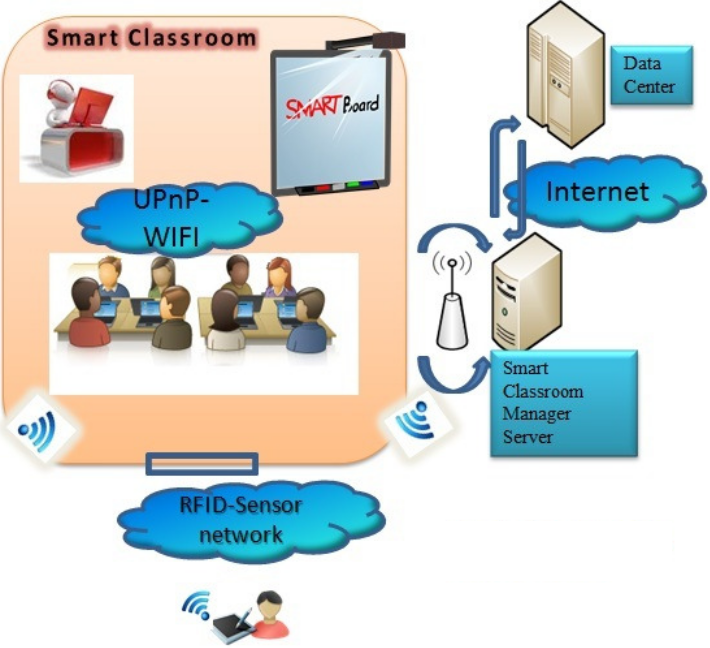
\includegraphics[width=0.6\linewidth]{imgs/Dekdouk2012}
	\caption{Sala de aula inteligente}
	\label{fig:Dekdouk2012}
\end{figure}

\cite{Gligoric:2012} apresentam um sistema de inferência da qualidade de uma palestra com ênfase na aplicação de Internet das Coisas (IoT) em Sala de Aula Inteligente. Neste trabalho é discutido como Inteligência de Ambientes pode ser usada para oferecer um \textit{feedback} automático e em tempo real da qualidade de uma palestra em auditório baseando-se em parâmetros. Utilizando sensores de ruído, \textit{Passive Infrared} (PIR), câmeras de vídeo e microfones. A inferência da qualidade da palestra é feita a partir do nível de interesse da plateia, que pode ser medido pela inquietação dos ouvintes e pelo ruído ambiente. 


% Após apresentados e discutidos alguns pontos dos trabalhos correlatos que abordam a construção de ambientes de internos de aprendizagem, nota-se que a abordagem proposta nesta dissertação se diferencia das pesquisas relacionadas expostas até o momento, especialmente no que diz respeito à materialidade do ambiente proposto. Nesta dissertação, trabalha-se igualmente na construção de um ambiente baseado em sala de aula presencial, mas, não se mantém o foco unicamente na construção de novos dispositivos ou aparatos físicos, como os trabalhos apresentados nesta Seção~\ref{section:wIndoorClassroom}. A maior parte das intervenções contidas no método proposto nesta dissertação, diz respeito à inserção de tecnologia usando o conceito de computação pervasiva, de modo que, a interação das pessoas com os dispositivos seja percebida como algo natural. Por isso, os diversos elementos de intervenção direta no ambiente de sala de aula propostos neste trabalho primam por utilizar equipamentos já existentes e muito utilizados no dia a dia, tais como, computadores pessoais, \textit{smartphones} e \textit{tablets}. Sendo assim, no sentido de construção de ambiente de sala de aula, a abordagem proposta tem também baixo custo de implantação, uma vez que é possível utilizar uma infraestrutura pré-existente em diversas escolas.

% % -----------------------------------------------------------------
% => Ambiente Externo
% -----------------------------------------------------------------

\subsection{Ambiente Externo de Aprendizagem}
\label{section:OutdoorClassroom}

\cite{Xue:2011} descrevem um \textit{framework} para criação de ambiente de aprendizado ubíquo baseado em Internet das Coisas e com três camadas: percepção, rede de computadores e aplicação. Apesar de não utilizar um sensor específico, este trabalho indica elementos que podem ser utilizados para construir um ambiente de aprendizado ubíquo e que seja integrado com qualquer sensor ou aplicação (Figura~\ref{fig:Xue2011}).

\begin{figure}[ht]
	\centering
	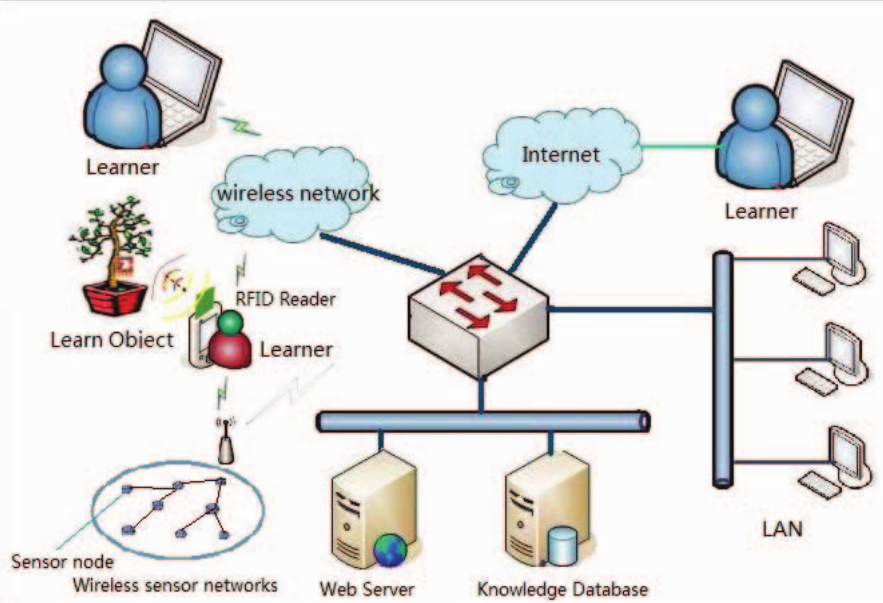
\includegraphics[width=0.9\linewidth]{imgs/Xue2011}
	\caption{Arquitetura do Sistema de Aprendizagem Ubíqua}
	\label{fig:Xue2011}
\end{figure}

\cite{Oluwagbemi:2014} apresentam uma revisão de literatura acerca das tendências da aplicação de métodos de computação pervasiva em ambientes de sala de aula apresenta trabalhos focados em \textit{3D Printing}, \textit{Quantified Self}, Assistentes Virtuais, Jogos e \textit{Gamification}. Como trabalhos futuros é sugerida a adoção e implementação de um modelo nigeriano de ambiente de aprendizado em sala de aula.

\cite{Dong:2007} apresentam um método de reconhecimento de contexto de aprendizagem baseado na Análise do Comportamento para recomendação de um calendário de estudos, quando o estudo é feito em casa, com o objetivo de incentivar o estudante a adquirir o hábito da aprendizagem. O trabalho utiliza sensores de RFID para detectar se os livros estão sobre a mesa de estudo e o sistema cruza essa informação com os dados dos professores e a demanda dos pais para considerar se o aluno está ou não em um contexto de aprendizagem. Se estiver, então, uma programação de estudos é feita pelo sistema. Entretanto, a avaliação do desempenho do sistema foi feita através de formulários aplicados aos estudantes, onde mais de 80\% concordou que o sistema proposto contribui para a melhoria do processo de aprendizado.

\cite{Tan:2007} propõem utilizar a tecnologia em ambientes de aprendizagem externa para ajudar num maior ganho educacional. Utilizando os conceitos de aprendizagem móvel, aprendizagem ubíqua e reconhecimento de contexto foi desenvolvido um sistema denominado "\textit{Ubiquitous Learning with Educational Resources}"~(EULER) baseado em RFID, Internet, redes sem fio, sistemas embarcados e tecnologias de Banco de Dados.

\begin{figure}[ht]
	\centering
	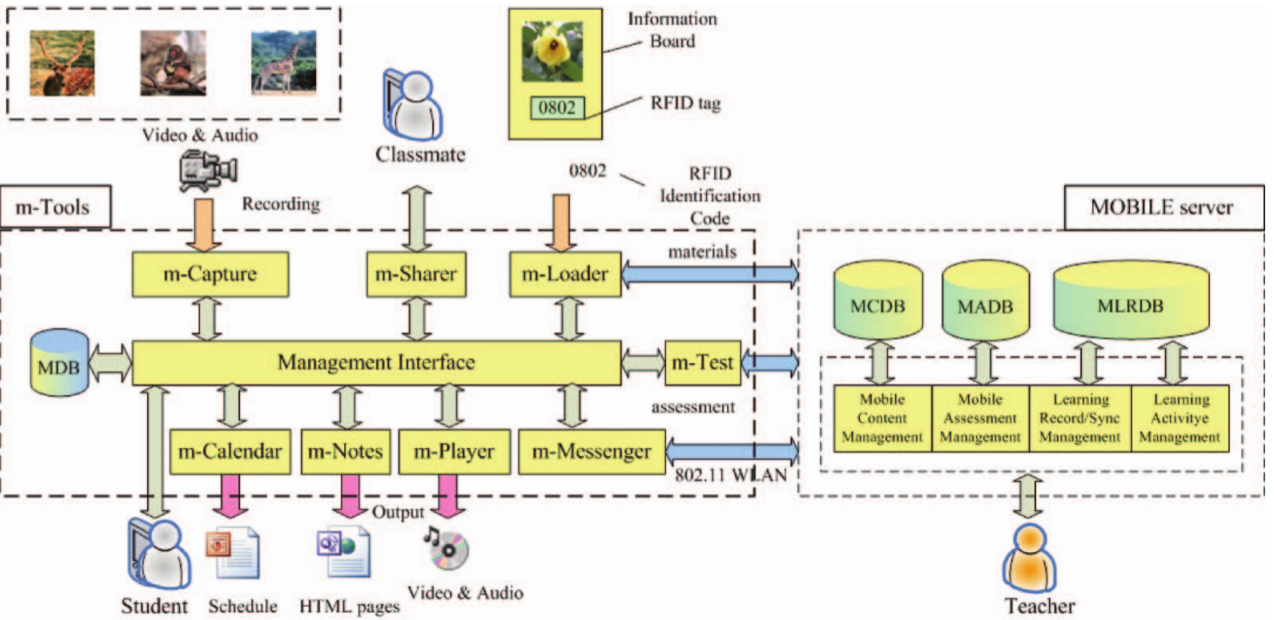
\includegraphics[width=0.8\linewidth]{imgs/Tan2007a}
	\caption{Estrutura do sistema EULER}
	\label{fig:Tan2007a}
\end{figure}

O sistema EULER consiste em dois subsistemas (Figura~\ref{fig:Tan2007a}): (a) Servidor "\textit{MObile-Based Interactive Learning Environment}"(MOBILE) para uso do professor; (b) ferramentas móveis para os estudantes (m-Tools). O professor prepara e armazena o material didático (que pode conter temas, imagens, áudios e descrição textual) no servidor, construindo as relações entre este e os códigos RFID. Os alunos podem coletar e compartilhar dados, além de editar artigos ao seu próprio critério. Dentre as ferramentas do \textit{m-Tools} que os estudantes podem usar estão: PDA, leitor RFID e câmera.

Com tudo configurado, a aula pode acontecer em qualquer ambiente externo, seja um museu, um zoológico ou um parque. A Figura~\ref{fig:Tan2007b} apresenta um cenário de uso do EULER no \textit{Guandu Nature Park} em Taiwan.

\begin{figure}[ht]
	\centering
	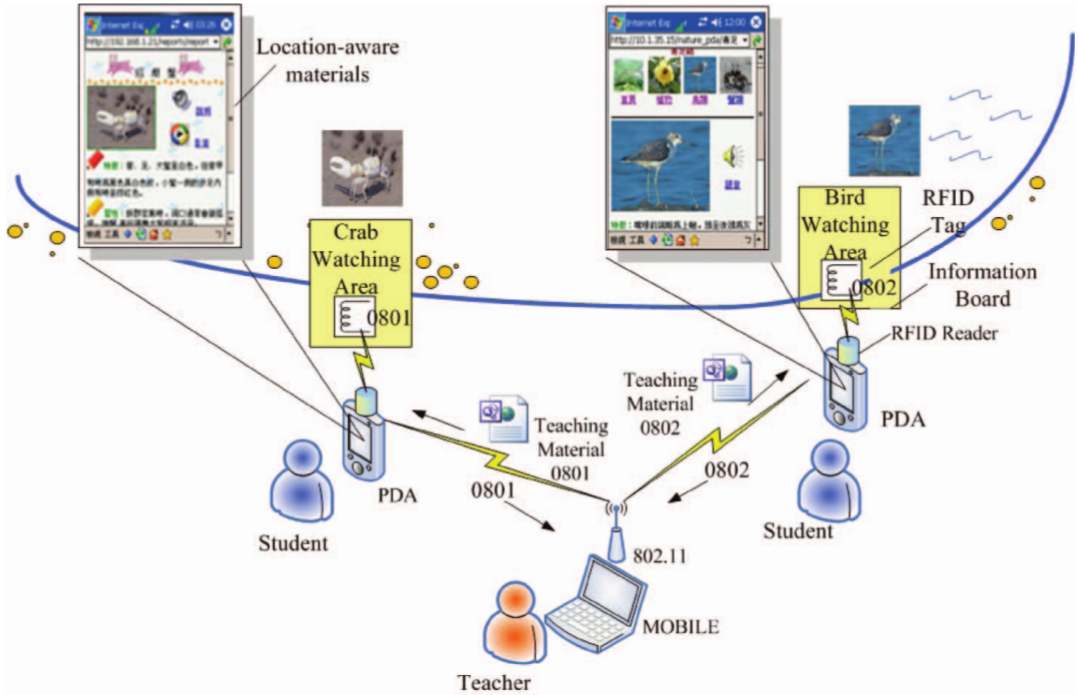
\includegraphics[width=0.9\linewidth]{imgs/Tan2007b}
	\caption{Cenário de uso do sistema EULER no Guandu Nature Park}
	\label{fig:Tan2007b}
\end{figure}

Os experimentos foram executados com dois grupos de 36 alunos cada e o auxílio de quatro professores experientes em educação com uso de computadores. Um grupo experimental utilizou o EULER e um grupo de controle recebeu instrução tradicional. Os experimentos foram divididos em quatro fases e foram aplicados testes antes, durante e depois dos experimentos, com exceção do pré-teste, os estudantes que utilizaram o EULER obtiveram maior desempenho em todos os testes das quatro fases.

% Após breve apresentação e discussão dos trabalhos correlatos à construção de ambientes externos de aprendizagem, nota-se que a abordagem proposta nesta dissertação tem grande proximidade, a maior parte desses trabalhos faz uso de metodologias de aprendizado ubíquo que permitem que a interação do estudante com o sistema seja a mais natural possível, mesmo em ambientes não controlados, como um museu ou um parque.

% É importante observar que, tanto os trabalhos voltados à construção de ambientes internos de aprendizagem, quanto os trabalhos que propõe metodologias para ambientes externos não apresentam: (i) ferramentas de apoio ao professor na fase de composição da aula; (ii) inserção de metodologias de ajuda sob demanda, especialmente, voltadas para a avaliação da aprendizagem dos estudantes; (iii) métricas de aprendizagem para análise \textit{a posteriori} do desempenho dos estudantes após a execução de uma aula. Outro fator importante consiste de que a maior parte dos trabalhos que fazem alguma análise de desempenho, voltam-se para avaliação do sistema baseada unicamente em formulários de opinião aplicados aos estudantes. A proposta apresentada neste trabalho é avaliada utilizando métricas de aprendizagem que possibilitem ao professor fazer análises, inferências e, assim, tomar decisões que impactem positivamente o desempenho dos estudantes. Desse modo, a eficácia do método proposto neste trabalho está ligada à sua capacidade de apresentar métricas que permitam ao professor fazer um diagnóstico da turma para tomadas de decisões relacionadas às metodologias utilizadas durante a execução da aula.

% %Achei que antes do resumo faltou você comentar (pode ser em um parágrafo) em que aspectos o teu trabalho vai acrescentar o estado-da-arte, principalmente quando comparado com os trabalhos correlatos.

\section{Ferramentas de Autoria de Objetos de Aprendizagem}
\label{sec:autoria}
%\label{section:author_performance_evaluation}

Ferramentas de autoria auxiliam nos processos de criação, inserção e utilização de objetos de aprendizagem como parte do material didático com o objetivo de facilitar o ensino-aprendizagem e, assim, contribuir com o engajamento e a construção do conhecimento por parte dos estudantes. Neste trabalho, o processo de autoria de objetos de aprendizagem, especialmente questionários avaliativos e objetos tangíveis, está a cargo do módulo Compositor (ver Seção \ref{section:composer}), de modo que esta seção apresenta alguns trabalhos relacionados a métodos e ferramentas de autoria.

Tendo em vista que pacotes de aplicativos para escritório contendo editores de texto, de planilhas ou de apresentação são amplamente difundidos e que, por isso, tais ferramentas podem ter seu uso facilmente direcionado para a criação de objetos de aprendizagem, \cite{Passos:2010} propõem a inserção de códigos em VBA (\textit{Visual Basic for Applications}) no Microsoft PowerPoint para criação de aplicações interativas que facilitem a aprendizagem dos conteúdos curriculares em escolas públicas de um município do interior do Estado do Amazonas~(Brasil).

\begin{figure}[htb]
	\centering
	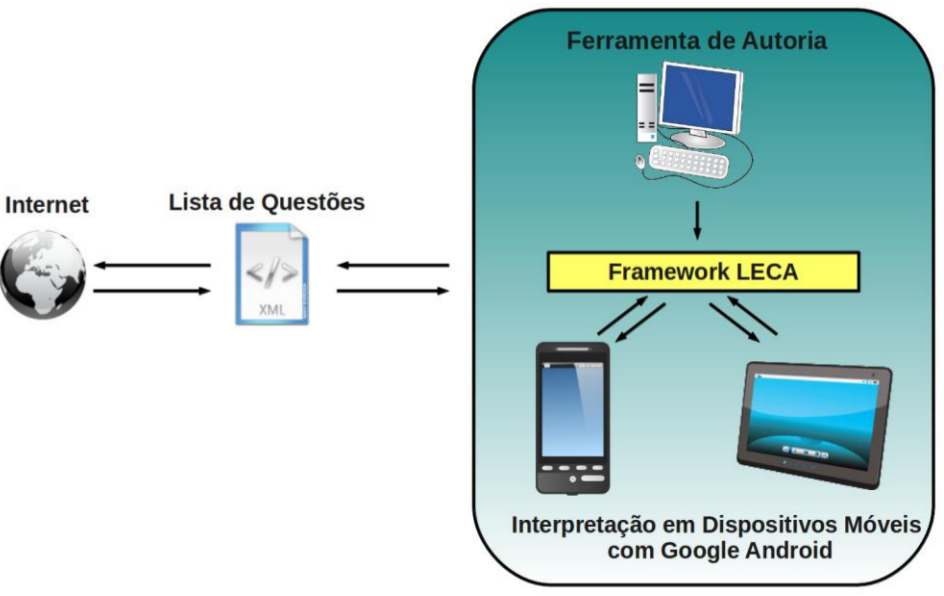
\includegraphics[width=0.8\linewidth]{chapters/works/orlandi2012.png}
	\caption{Arquitetura do LECA. Fonte:~\cite{Orlandi:2012}}
	\label{fig:orlandi2012}
\end{figure}

\cite{Orlandi:2012} apresentam uma ferramenta de autoria para dispositivos móveis chamada LECA (Lista de Exercícios com Correção Automática), focada na criação e na responsividade de listas de exercícios de múltipla escolha com avaliação do desempenho do aluno através de pontuação. A Figura~\ref{fig:orlandi2012} apresenta o diagrama da relação do \textit{framework} do LECA com as aplicações diversas, onde nota-se que o sistema é composto por uma parte de autoria das questões e por outra de visualização.

\begin{figure}[htb]
	\centering
	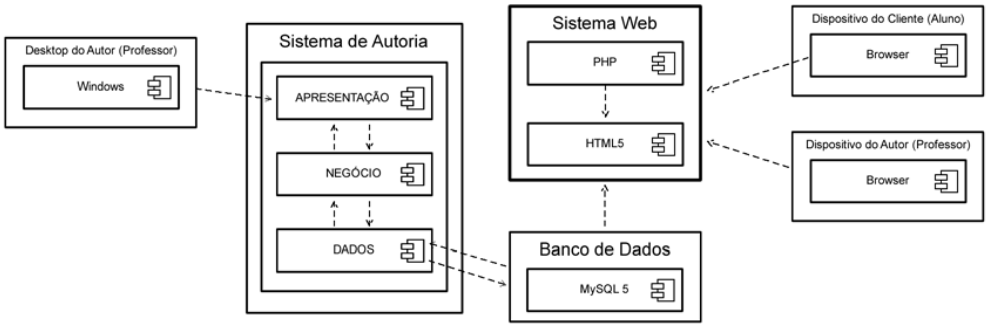
\includegraphics[width=0.8\linewidth]{chapters/works/guterres2014.png}
	\captionsetup{justification=centering}
	\caption{Estrutura da Plataforma ``Fábrica de Objetos''. \\Fonte:~\cite{Guterres:2014}}
	\label{fig:guterres2014}
\end{figure}

\cite{Guterres:2014} descrevem uma plataforma para construção de objetos de aprendizagem com foco em usuários com pouco conhecimento de informática. A plataforma apresentada foi implementada usando tecnologias web, dentre elas: HTML5, CSS e JQuery. A Figura~\ref{fig:guterres2014} ilustra o diagrama de componentes desta plataforma, onde pode-se observar que ela tem duas partes principais: (a) Sistema de Autoria e (b) Sistema Web com Banco de Dados. Onde o Sistema de Autoria é o responsável de fato pela criação, modificação ou remoção dos objetos de aprendizagem ou das páginas que os compõem e o Sistema Web permite o gerenciamento destes OAs. Além disso, cada objeto de aprendizagem existente no repositório é organizado conforme ilustrado na Figura~\ref{fig:guterres2014_objetos}.

\begin{figure}[htb]
	\centering
	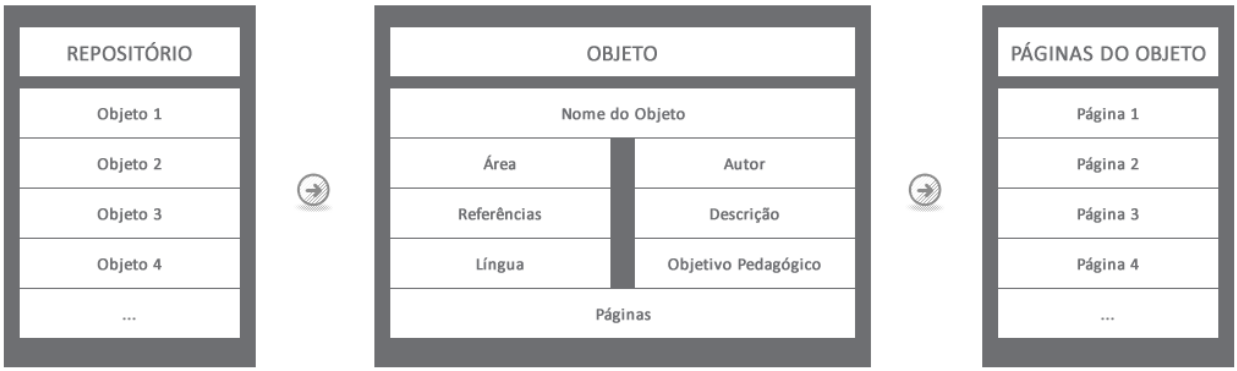
\includegraphics[width=1\linewidth]{chapters/works/guterres2014_objetos.png}
	\captionsetup{justification=centering}
	\caption{Estrutura dos OAs na plataforma ``Fábrica de Objetos''. \\Fonte:~\cite{Guterres:2014}}
	\label{fig:guterres2014_objetos}
\end{figure}


%\cite{Flores:2011}, baseando-se em Kolb, Gagné e Wiley, definem um conjunto de funcionalidades que precisam estar presentes em uma ferramenta de autoria para a construção de objetos de aprendizagem mais adequados. Além disso, apresentam um exemplo de criação e aplicação de um objeto de aprendizagem para ensino de matemática usando a ferramenta gratuita eXeLearning. Dentre as funcionalidades descritas no artigo, destacamos: \textit{Applet Java}, Apresentação em \textit{Slides}, Textos, Imagens, Questionários de múltipla escolha ou verdadeiro-falso, entre outros.

\section{Ferramentas e Métricas de Avaliação do Desempenho}\label{sec:avaliacao}
%\label{sec:related-avaliacao-aprendizagem}

As novas tecnologias possibilitam obter dados de interação dos estudantes ao longo do processo de aprendizagem, permitindo gerar gráficos e análises que auxiliem o professor na avaliação e na tomada de decisões que envolvam, por exemplo, a adição de atividades pedagógicas que reforcem o aprendizado de um conteúdo, e é considerada uma estratégia pedagógica mais eficiente.
Assim, dados obtidos de aulas e avaliações podem permitir melhores inferências relacionadas ao perfil de aprendizagem e às dificuldades de uma determinada turma ou de um único estudante. Desta forma, o sistema pode recomendar diversas atividades e estratégias que sejam mais adequadas e adaptadas às reais necessidades da classe ou aluno.

Além disso, há ainda pesquisas relacionadas ao desenvolvimento de métricas e ferramentas específicas para a avaliação do desempenho dos estudantes a fim de melhorar o acompanhamento da aprendizagem por parte do professor. 
Assim, esta seção apresenta alguns trabalhos correlatos a avaliação da aprendizagem de estudantes em situação escolar.

%Avaliação do desempenho
%\cite{Malvezzi:2010} introduzem uma ferramenta para avaliação de alunos em cursos presenciais mediados por tecnologia aplicando a Teoria \textit{Fuzzy} em variáveis de interação como \textit{chat}, fórum, tarefas e testes. 

\subsection{WebMonitor - monitoramento e acompanhamento}
\cite{Lucena:2015} propõem uma ferramenta para monitoramento de desempenho em um Ambiente Virtual de Aprendizagem (AVA) chamada o WebMonitor, que funciona como um \textit{plugin} para monitoramento de \textit{logs} de tarefas e participação em fóruns do Moodle.

\begin{figure}[htb]
	\centering
	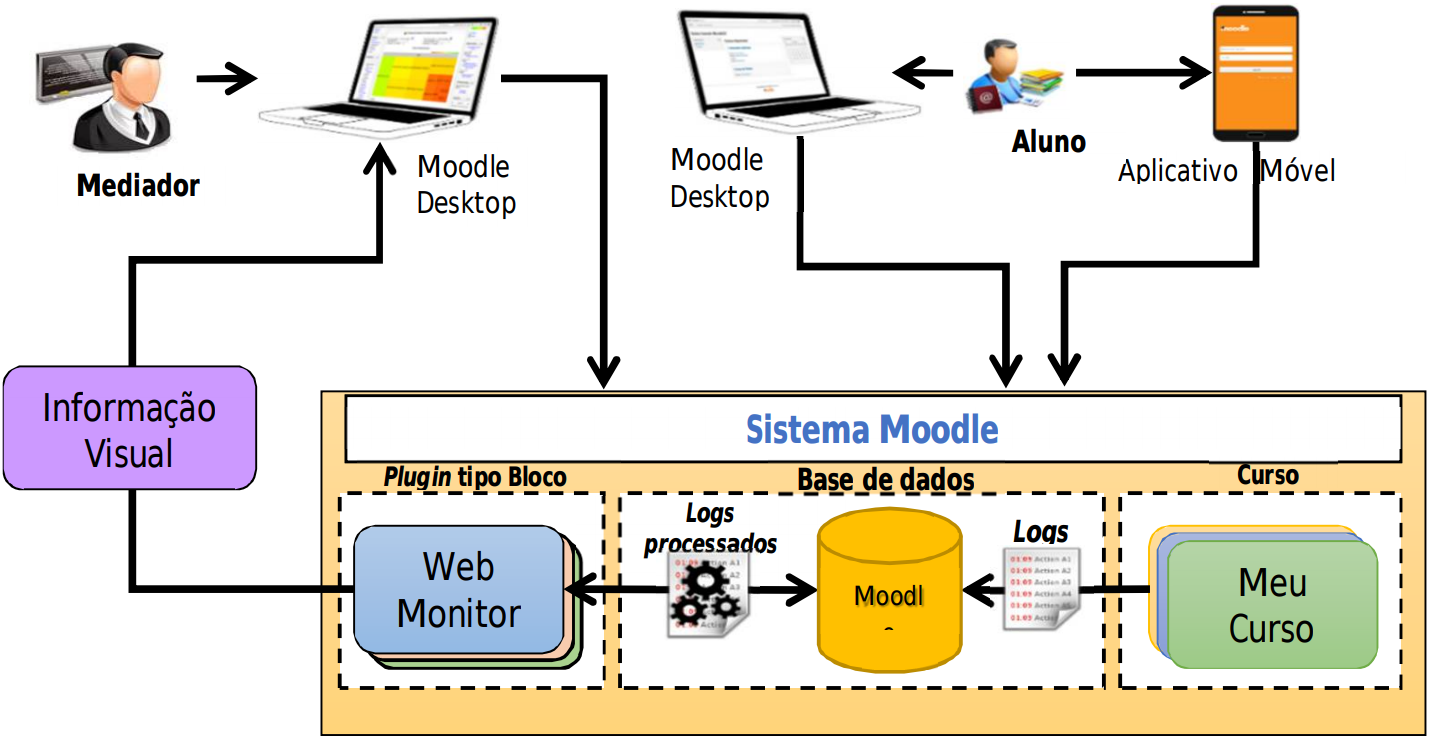
\includegraphics[width=0.9\linewidth]{chapters/works/Lucena2015_5162-6882-1-PB_arquitetura.png}
	\caption{Arquitetura do WebMonitor. Fonte:~\cite{Lucena:2015}}
	\label{fig:Lucena2015_Arquitetura}
\end{figure}

A Figura~\ref{fig:Lucena2015_Arquitetura} apresenta a arquitetura da ferramenta, cujo fluxo de informações pode ser resumido em cinco passos~\citep{Lucena:2015}: 
\begin{enumerate}
    \item Acesso ao AVA Moodle pelos estudantes (via Desktop ou dispositivo móvel);
    \item Moodle coleta as ações dos usuários e as registra em um log;
    \item Mediador acessa o WebMonitor instalado no Moodle;
    \item WebMonitor recupera e processa os dados de logs da base de dados do Moodle;
    \item A informação processada é transformada visualmente e disponibilizada ao mediador através de representações gráficas (\textit{Treemaps} e gráficos de barras).
\end{enumerate}

Desse modo, o monitoramento é realizado utilizando a técnica \textit{Treemap} para visualização da informação a fim de auxiliar o professor na percepção do desempenho acadêmico e do comportamento dos estudantes em atividades como postagem de arquivos e interações em fóruns de discussão, o que, segundo os autores, possibilitaria melhores condições de identificar possíveis desistências, reprovações ou evasão de
estudantes por parte dos professores ou mediadores. Na Figura~\ref{fig:Lucena2015}, o WebMonitor exibe as interações de um aluno.

\begin{figure}[htb]
	\centering
	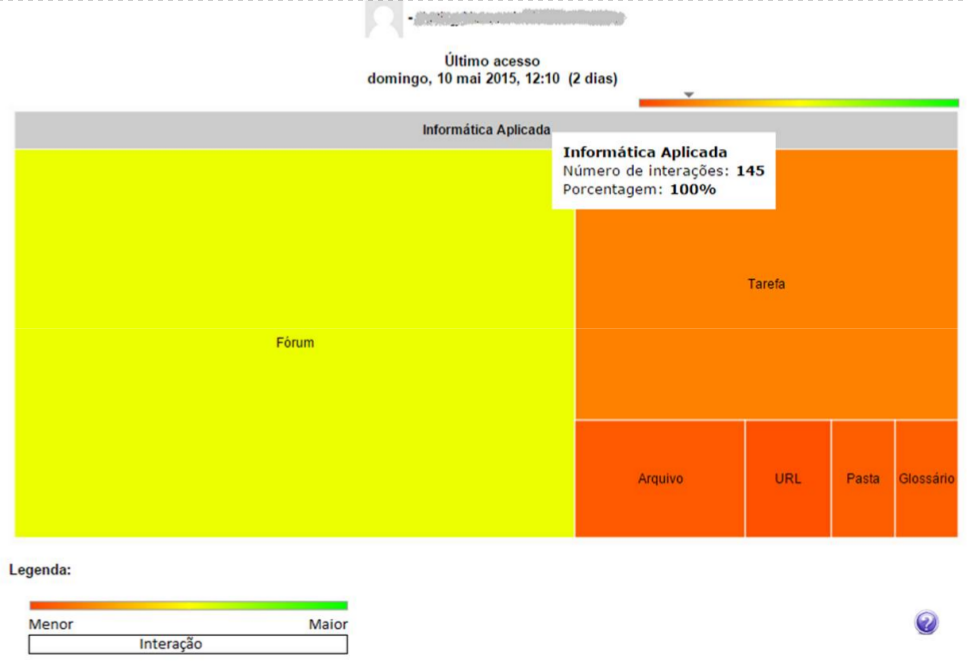
\includegraphics[width=0.9\linewidth]{chapters/works/Lucena2015.png}
	\captionsetup{justification=centering}
	\caption{Exemplo do Treemap das interações de um estudante. \\Fonte:\cite{Lucena:2015}}
	\label{fig:Lucena2015}
\end{figure}

\subsection{Metodologia para \textit{Learning Analytics}}

Com enfoque em cursos semipresenciais ou híbridos, \cite{Nunes:2016} propõem uma metodologia de avaliação onde o desempenho é calculado a partir das notas e da participação do aluno. 

De acordo~\cite{Nunes:2016}, o processo de \textit{Learning Analytics} consiste nos cinco passos seguintes: (1) Capturar dados; (2) Reportar dados; (3) Predizer; (4) Adaptar; (5) Personalizar; e (6) Intervir. Além disso, as técnicas utilizadas para a realização de \textit{Learning Analytics} podem ser: (i) análises de redes sociais; (ii) processamento de linguagem natural; (iii) predição; (iv) determinação de risco; (v) sequenciamento de curso; e (vi) identificação de alunos que precisam de ajuda.

Assim, a proposta apresentada por~\cite{Nunes:2016} apresenta como critério avaliativo, para cada aluno, o cálculo de uma Nota Final (NF), a partir da Equação~\ref{equacao:nunes2016}. Onde, PT é dada pela ``Participação da Turma'', seja virtual (fóruns, mensagens e \textit{chats}), seja presencial (assiduidade, resolução de exercícios em sala, cumprimento de prazos de entrega); AE são ``Atividades Executadas'' e PE é a nota da ``Prova Escrita''. 

Como \textit{feedback}, são apresentados gráficos de quantidade de alunos aprovados e reprovados por turma (Figura~\ref{fig:Nunes2016}), relação entre a nota da participação virtual ou presencial e o número de acessos por turma.

\begin{equation}\label{equacao:nunes2016}
NF = \frac{(PT + AE + (PE*2)}{4}
\end{equation}

\begin{figure}[htb]
	\centering
	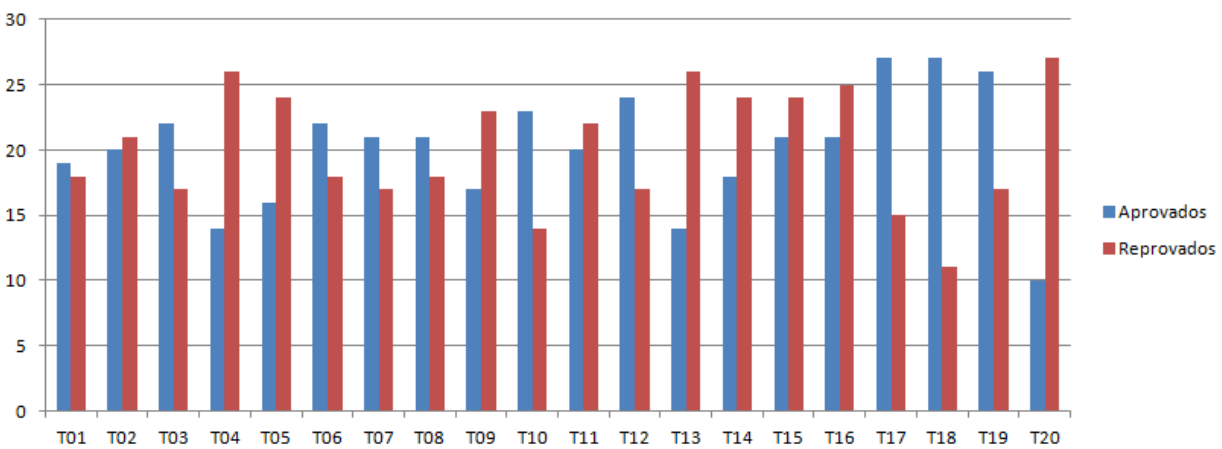
\includegraphics[width=1\linewidth]{chapters/works/Nunes2016.png}
	\captionsetup{justification=centering}
	\caption{Alunos Aprovados e Reprovados por Turma}
	\label{fig:Nunes2016}
\end{figure}

\subsection{Métricas de Desempenho para Estudantes e Professores}
\label{sec:level-understanding}

Um conjunto de métricas que leva em consideração o histórico de atividades dos estudantes foi descrito por~\cite{Biswas:2007}, são eles: (a) Nível de Compreensão, (b) Taxa de Aprendizagem do Aluno e, (c) Nível de dificuldade de um elemento de ontologia (assunto, tópico ou conceito).

\textbf{Nível de Compreensão (Equação~\ref{eq:lu})} é uma métrica que quantifica a relação entre diferentes índices de dificuldade, tempo de resposta e desvio. Os \textbf{índices de dificuldade} (tópico, conceito e questão) são descritos na Tabela~\ref{tab:Lu}.
O \textbf{tempo de resposta} é aplicado para capturar os chutes do estudante e deve ser comparado com o tempo de resposta esperado fornecido pelo autor da questão. Existem duas classes de Tempo de Resposta, a classe ``chute'' com valor 5 e a ``resposta normal'' (ou opinião fundamentada), cujo valor é 1.
O parâmetro \textbf{desvio} é dado de acordo com a classificação de resposta mostrada na Tabela ~\ref{tab:Weight_Biswas}, onde 0 significa que é uma resposta ``completamente incorreta'' e 5 corresponde a resposta ``perfeita'', ou seja, a resposta correta.

\begin{equation}\label{eq:lu}
L_u = \frac{IDT \cdot IDC \cdot IDQ \cdot Desvio}{Tempo \ de \ Resposta}
\end{equation}

\begin{table}[htbp]
\centering
\caption{O índice de dificuldade significa o quão difícil é uma questão ou tópico.}
\begin{center}
\begin{tabular}{|l|c|c|c|}
\hline
\textbf{Índice de Dificuldade} & \textbf{Fácil} & \textbf{Normal} & \textbf{Difícil} \\\hline
Índice de Dificuldade do Tópico (IDT) & 1 & 3 & 5 \\\hline
Índice de Dificuldade do Conceito (IDC) & 1 & 3 & 5 \\\hline
Índice de Dificuldade da Questão (IDQ) & 1 & 3 & 5 \\\hline
\end{tabular}
\end{center}
\label{tab:Lu}
\end{table}

\cite{Biswas:2007} enfatizam que os valores das Tabelas~\ref{tab:Lu}, \ref{tab:Weight_Biswas} e do ``Tempo de Resposta'' não foram derivados matematicamente, mas eles são aplicados apenas para diferenciar as distintas classes de estudantes. Nesse caso, é possível escolher quaisquer outros valores.

\begin{table}[htbp]
\caption{Valor do parâmetro Desvio}
\centering
\begin{tabular}{|c|c|c|c|c|c|}
\hline
\textbf{Desvio} & \textbf{Não tem ideia} & \textbf{Abaixo do Meio} & \textbf{Meio} & \textbf{Quase correto} & \textbf{Correto} \\ \hline
\textbf{Valor} & 0 & 2 & 3 & 4 & 5\\ \hline
\end{tabular}
\label{tab:Weight_Biswas}
\end{table}

Para estabelecer a métrica \textbf{Taxa de Aprendizado do Estudante ($SLR$)}, \cite{Biswas:2007} introduzem a definição de ``Pontuação do Estudante'', definida por $SS (s,i,o)$, que diz sobre a pontuação de um estudante $s$ em uma $i$-ésima avaliação em relação a um elemento ontológico $o$, onde esta ontologia pode ser uma disciplina, tópico ou conceito.
Assim, a taxa de aprendizado do estudante é a melhoria, na média, na pontuação de um estudante com respeito ao conjunto de avaliações. Isso permite a observação da evolução contínua e é expressa pela Equação~\ref{eq:student_rate}, onde $N$ é o total de questões acerca do elemento ontológico $o$, e $i$ é uma variável que expressa uma avaliação específica.

\begin{equation}\label{eq:student_rate}
\begin{split}
SLR(s,o) =  \frac{\sum \{(SS(i+1)-SS(i)) \cdot |SS(i+1)-SS(i)| \} }{N-1}
\end{split}
\end{equation}

%\noindent onde $N$ é o total de questões acerca do elemento ontológico $o$, e $i$ é uma variável que expressa uma avaliação específica.

Finalmente, \cite{Biswas:2007} definem que o \textbf{Nível de Dificuldade ($DL$)} de um elemento ontológico $o$ pode ser quantificado para todo $s$ através da Equação~\ref{eq:DL}.

\begin{equation}\label{eq:DL}
DL(o) = \overline{SLR}(s,o)
\end{equation}

\subsection{Modelo \textit{Learning Vectors} para \textit{Moodle}}
\label{sec:learningvectors}

\begin{figure}[htb]
	\centering
	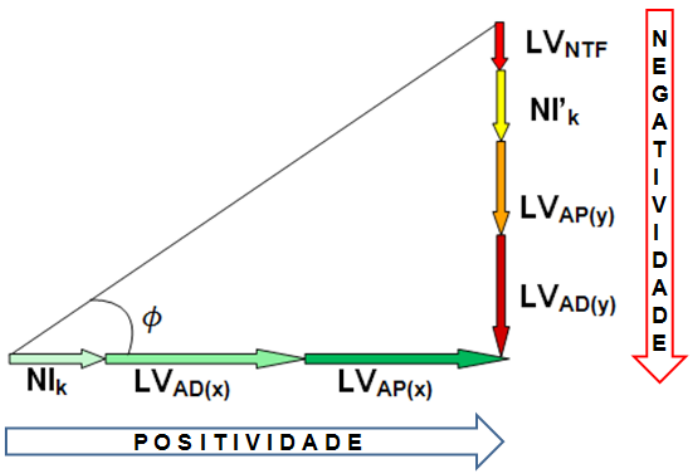
\includegraphics[width=0.45\linewidth]{chapters/works/Sales2019_LearningVectors_FatorB2.png}
	\caption{Representação do Vetor-Aprendizagem. Fonte:\cite{sales:2019}}
	\label{fig:Sales2019fatorbeta}
\end{figure}

\cite{sales:2019} apresentam uma ferramenta para Avaliação Formativa no AVA Moodle através de \textit{emoticons} e GIFs animados que alimentam um modelo baseado em Vetores-Aprendizagem. Os \textit{emoticons} e GIFs compõem uma escala iconográfica que os associa às seguintes menções qualitativas: ``muito bom'', ``bom'', ``regular'', ``fraco'', ``não satisfatório'' e ``neutro'' com o objetivo de alimentar um modelo matemático que leva em consideração as interações dos alunos em fóruns de discussão, tarefas, wikis e salas de chats para gerar pontuações, permitindo também a importação de notas de quizzes e o gerenciamento da frequência dos alunos.

A Figura~\ref{fig:Sales2019} apresenta o modelo proposto por~\cite{sales:2019}, onde, através de uma escala de menções qualitativas baseada na Escala Likert associada ao uso de \textit{emoticons} e GIFs, o professor/tutor avalia as interações dos alunos nas diversas atividades dentro do Moodle. Com essas avaliações, é possível calcular os vetores de aprendizagem (Figura~\ref{fig:Sales2019fatorbeta}) de modo que as projeções horizontais (LVx) e verticais (LV{y}) do vetor expressam, de um lado, a positividade de desempenho do aluno e a nota da atividade e, de outro, a negatividade do desempenho, respectivamente.

\begin{figure}[htb]
	\centering
	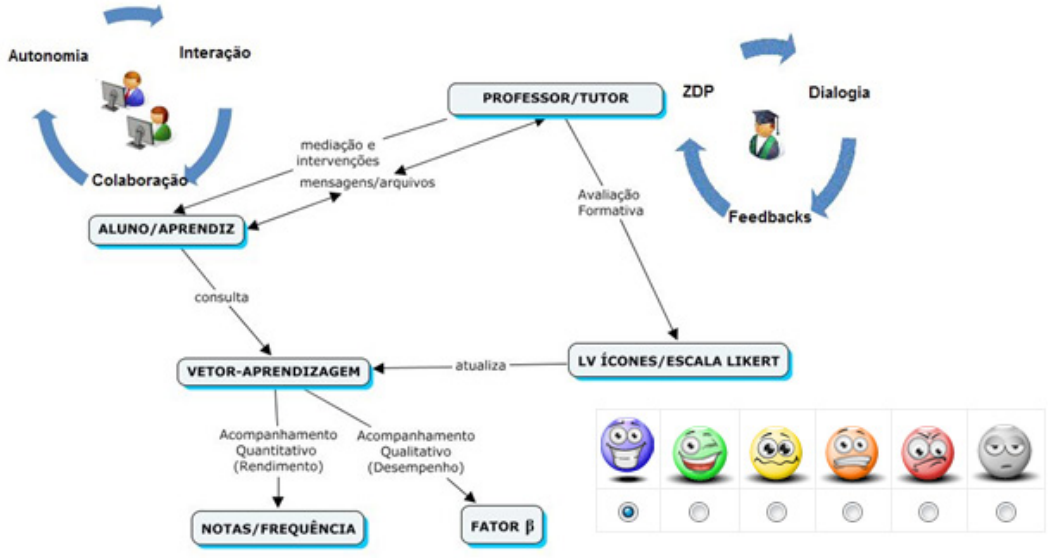
\includegraphics[width=1\linewidth]{chapters/works/Sales2019_LearningVectors.png}
	\captionsetup{justification=centering}
	\caption{Modelo de Avaliação usando Learning Vectors. \\Fonte:~\cite{sales:2019}}
	\label{fig:Sales2019}
\end{figure}

Além disso, em um trabalho anterior, \cite{sales:2012} especificam que a Positividade ($P$), dada pela Equação~\ref{eq:Positividade}, é o somatório das projeções horizontais dos vetores de aprendizagem $LV_{AD(x)}$ de atividades a distância (fóruns, chats, tarefas e wikis) e $LV_{AP(x)}$ de atividades presenciais, acrescido do número de interações positivas $NI_k$ ponderadas e categorizadas pelo professor/tutor como ``muito bom'' (peso 3 - azul), ``bom'' (peso 2 - verde) e ``regular'' (peso 1 - amarelo).

\begin{equation}
	\label{eq:Positividade}
	P = \sum_{x}^{i=1} LV_{ADi} +  \sum_{y}^{j=1} LV_{APj} + \sum_{z}^{k=1} NI_k
\end{equation}

Por sua vez, a Negatividade ($N$), expressa na Equação~\ref{eq:Negatividade}, é o somatório das projeções verticais dos vetores de aprendizagem $LV_{AD(y)}$ e $LV_{AP(y)}$, acrescido do somatório do número de interações negativas $NI'_k$ categorizadas como ``fraco'' (peso 1 - laranja) ou ``não satisfatório'' (peso 2 - vermelho) e do número total de faltas, dado por $LV_{NTF}$~\citep{sales:2012}.

\begin{equation}
	\label{eq:Negatividade}
	N = \sum_{x}^{i=1} LV'_{ADi} +  \sum_{y}^{j=1} LV'_{APj} + \sum_{z}^{k=1} NI'_k + LV_{NTF}
\end{equation}

Dados os vetores ortogonais de positividade e negatividade, é calculado o ``Fator $\beta$'', que é dado por $\nicefrac{P}{N}$ e é o indicador qualitativo não linear do nível de desempenho dos alunos~\citep{sales:2012}.

\section{Resumo}
Neste capítulo, descrevemos e analisamos diversos trabalhos relacionados com a criação e utilização de manipulativos físicos e virtuais no contexto educacional, tais trabalhos têm em comum o enfoque somente em uma ou no máximo duas fases do processo de ensino-aprendizagem. Assim, a maioria dos trabalhos propõe objetos de aprendizagem físicos ou virtuais juntamente com um ambiente de utilização especializado~\citep{zacharia:2011, Salehi:2014, ha:2018, Blikstein:2012, Blikstein2016, Azad:2016, imamura:2018}, mas, poucos fazem avaliação da aprendizagem~\citep{zacharia:2011,Salehi:2014,ha:2018} e nenhum dos trabalhos propõe efetivamente uma avaliação da aprendizagem que leve em consideração dados de interação dos alunos com objetos físicos/virtuais.

Os trabalhos de \cite{Santos:2014, imamura:2018, lima:2016, gluz:2018}, que abordam diretamente o contexto de objetos tangíveis e de ambientes físico-digitais, apesar de conterem elementos embrionários que podem ser aproveitados como inspiração para a construção de um ambiente tangível de aprendizagem, não apresentam abordagens formais para descrição e padronização de objetos tangíveis de modo que possam ser integrados a um ambiente de aprendizagem coerente que possibilite o registro e a análise de dados de interação dos estudantes e, por conseguinte, a avaliação da experiência de aprendizado, de modo que seja possível propor ações pedagógicas voltadas a melhoria dessa experiência.

Além disso, a maioria dos trabalhos focados somente na autoria de objetos de aprendizagem em geral~\citep{Passos:2010, Orlandi:2012, Guterres:2014}, não levam em consideração a criação de objetos que sejam ao mesmo tempo físicos e virtuais/digitais.

%Embora \cite{Santos:2014} e~\cite{santos:2014ambientes} conceituem vários aspectos relativos a criação de ambientes físico-virtuais de aprendizagem e apresentem uma proposta de implementação, seus trabalhos não discorrem sobre os principais desafios acerca da construção e utilização plenas de objetos físico-virtuais tais como o registro e a análise da interação dos estudantes com tais objetos, de modo a avaliar a experiência de aprendizado e propor ações pedagógicas voltadas a melhoria dessa experiência. Além disso, permanecem os problemas relacionados a sistematização dos metadados ou de uma ontologia para esses objetos, visto que inexiste uma proposta nesse sentido. Vale ressaltar que tais problemas de descrição e padronização dificultam o reuso desses objetos, bem como a avaliação da aprendizagem quando da inserção dos mesmos em uma aula apoiada por tecnologia.

Por fim, este capítulo apresentou trabalhos e ferramentas que abordam a questão da avaliação em ambientes virtuais de aprendizagem~\citep{Lucena:2015, Nunes:2016, Biswas:2007, sales:2012, sales:2019}. Entretanto, apenas~\cite{Biswas:2007} e~\cite{sales:2012} apresentam novas métricas ou modelos para verificação do desempenho dos estudantes nesses ambientes. Além disso, nenhum dos trabalhos leva em consideração o uso de objetos físico-digitais de aprendizagem.

% Os trabalhos apresentados aqui %, sobre ferramentas de autoria, criação de ambientes de aprendizagem ou avaliação da aprendizagem, 
% têm em comum o enfoque em somente uma ou no máximo duas fases do processo de ensino-aprendizagem. Assim, ora há trabalhos que abordam a criação de objetos de aprendizagem juntamente com um ambiente para utilização, ora há trabalhos que apresentam ferramentas que apenas geram tais objetos. Da mesma forma, a maioria dos trabalhos apenas agrega ferramentas de avaliação a ambientes pré-existentes ou abstraem o ambiente que executará os OAs. Além disso, na literatura, poucos trabalhos focados em avaliação de desempenho do estudante introduzem novas métricas de avaliação, como~\cite{Biswas:2007} e~\cite{sales:2012} apesar de alguns introduzirem novas formas de visualização de resultados, como faz~\cite{Lucena:2015}.

Desse modo, a plataforma a ser apresentada nesta Tese, ao abranger as três fases de Autoria, Condução e Avaliação de uma aula, %de modo simples e eficiente, 
almeja contribuir com os esforços de aprimoramento destes processos através da inserção de recursos computacionais tangíveis em um ambiente de aprendizagem de modo que possam ser utilizados de forma integrada aos objetos de aprendizagem já existentes, além de possibilitar avaliação/acompanhamento da aprendizagem de uma forma diferenciada.

% -----------------------------------------------------------------
% => SYSTEMATIC REVIEW - 4 [DOING]
% -----------------------------------------------------------------
%% 
%\input{chapters/sysreview_inv.tex}

% -----------------------------------------------------------------
% => PROPOSED METHOD - 5 [DOING]
% -----------------------------------------------------------------
%% 
% -----------------------------------------------------------------
% => PROPOSED METHOD 
% -----------------------------------------------------------------

% \chapter{Verificações Simplificadas e Demonstração de Erros em Código C} \label{Chap:prosedMethod}
\chapter{Método Proposto} \label{Chap:prosedMethod}

Este capítulo descreve a arquitetura e as ferramentas propostas por este trabalho para a criação de um ambiente de educação apoiada por tecnologia que permita a inserção e o uso de objetos tangíveis de aprendizagem, além de métricas para acompanhamento e avaliação da aprendizagem que auxiliem o professor e os estudantes ao longo do processo de ensino-aprendizagem.

\cite{Zilse:2016} afirmam que o processo de educação em sala de aula tem duas fases principais: (1) Composição da aula e (2) Execução da aula. Na fase de execução, há a possibilidade de avaliação da aula a partir de \textit{feedbacks} que o professor obtém através de comentários, comportamentos ou mesmo dos questionários que ele aplicou aos estudantes. Assim, o Modelo apresentado nesta Tese, consiste em uma arquitetura composta por quatro módulos que interagem entre si: (1) \textit{Compositor}, (2) \textit{Servidor}, (3)  \textit{Player} e (4) \textit{Analytics}.

\begin{figure}[htb]
\centering
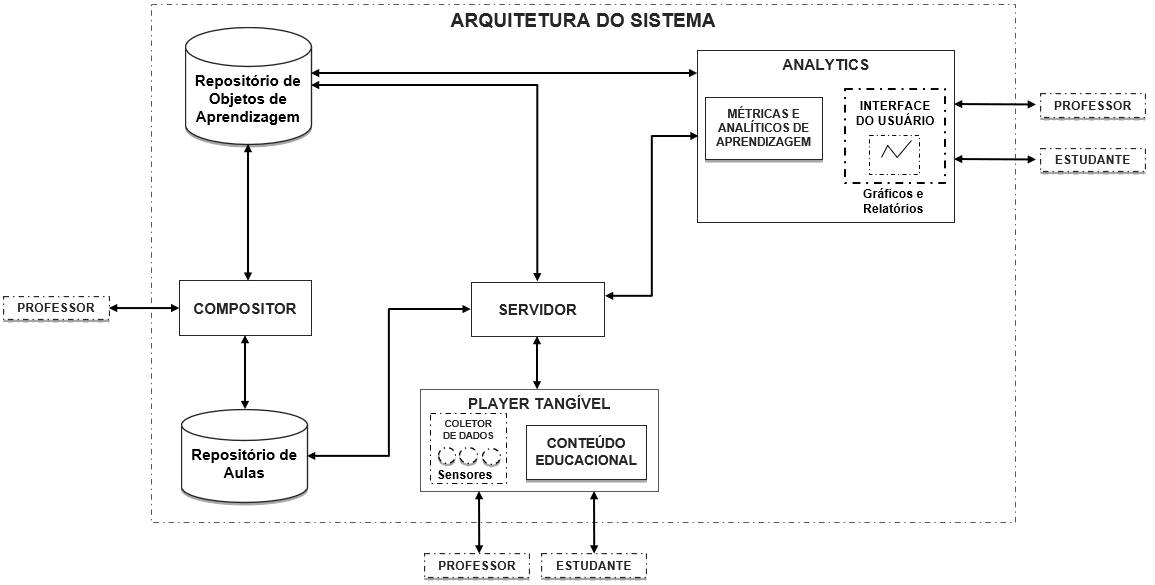
\includegraphics[width=1\linewidth]{chapters/proposedMethod/arquitetura_v4_1.png}
\caption{Arquitetura da Plataforma proposta}
\label{fig:arquitetura}
\end{figure}

De acordo com o Modelo apresentado na Figura~\ref{fig:arquitetura}, pode-se perceber que o professor interage e atua no ambiente educacional durante todo o processo, isto é, da composição e execução da aula até a visualização dos gráficos ou analíticos de aprendizagem gerados pelas interações dos estudantes com o conteúdo educacional, que acontecem apenas durante a aula e, sempre, mediadas pelo \textit{Player}.

Este capítulo é dividido em 4 seções. A primeira descreve o Compositor, os tipos de objetos de aprendizagem que são aceitos para a elaboração de uma aula, além da proposta de inclusão de objetos tangíveis de aprendizagem. A segunda seção apresenta o Servidor, que é responsável por agregar e armazenar os dados da interação dos estudantes com os dispositivos. Após isso, é apresentada a arquitetura do Player, que é responsável pela execução da aula, propriamente dita, e pela coleta dos dados de interação. Além de uma proposta de adição de objetos tangíveis de aprendizagem que permita interação entre suas partes física e digital. Por fim, a quarta seção aborda as métricas e analíticos de aprendizagem, ou seja, a parte do sistema responsável pelas análises dos dados e pela construção de gráficos para ajudar em tomadas de decisão que mais ajudem os estudantes nos processos de ensino-aprendizagem. %E, finalmente, a quinta seção apresenta um novo componente que serve de interface entre os módulos \textit{Servidor} e \textit{Analytics} e que aciona agentes que deem notificações ou façam recomendações adaptadas às percepções de contexto do estudante e às suas necessidades pedagógicas.
% , onde tais percepções e necessidades serão recebidas do componente analíticos.


\section{Compositor}\label{section:composer}
Essencialmente, este módulo atua como ferramenta e repositório de aulas e objetos de aprendizagem, de modo que é o responsável pela composição das aulas a partir de objetos de aprendizagem criados e/ou inseridos pelo professor, podendo também receber objetos provenientes de outros repositórios. É importante salientar que, em especial, o compositor permite a geração de objetos de aprendizagem como questionários avaliativos de múltipla-escolha e tangíveis. Outros objetos como slides, vídeos e imagens podem ser inseridos/trocados e utilizados na composição de uma aula, mas não podem ser editados pela ferramenta.

Para organização do sistema, foi criada uma hierarquia em que o maior nível é o da `Disciplina', dentro dele são cadastradas várias `Aulas', onde cada aula pode conter objetos de aprendizagem de diversos tipos. Além disso, estes objetos também estão ligados às disciplinas e a um professor que pode exercer o papel de autor desse objeto.

% %A Figura~\ref{fig:composerhierarquia} mostra a parte do Diagrama Entidade Relacionamento (Diagrama ER), que descreve a relação entre as entidades do banco de dados do Compositor. No extrato em questão, pode-se visualizar as entidades: \textit{user},\textit{Disciplina}, \textit{Aula} e \textit{Capitulo}.

% %\begin{figure}[h]
% %	\centering
% %	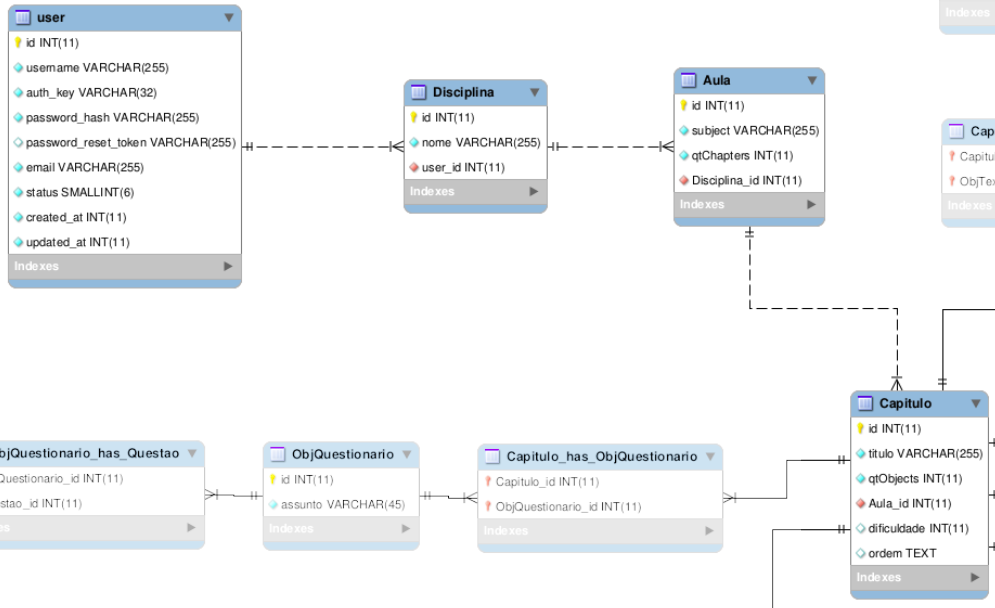
\includegraphics[width=1\linewidth]{imgs/ERComposer_hierarquiav2}
% %	\caption{Composer: entidades base}
% %	\label{fig:composerhierarquia}
% %\end{figure}

A Figura~\ref{fig:arquitetura_compositor} apresenta os principais componentes do Compositor, divididos em duas partes: (i) `Repositório de Aulas', onde é possível visualizar as entidades \textit{Disciplina}, \textit{Aula} e \textit{Objetos de Aprendizagem}, e (ii) `Repositório de Objetos de Aprendizagem', onde os objetos incluídos em uma aula podem ser acessados diretamente do banco de dados, especialmente, quando há reutilização de um objeto já armazenado. Além disso, há um destaque para a integração de objetos tangíveis de aprendizagem na plataforma.

\begin{figure}[htb]
	\centering
	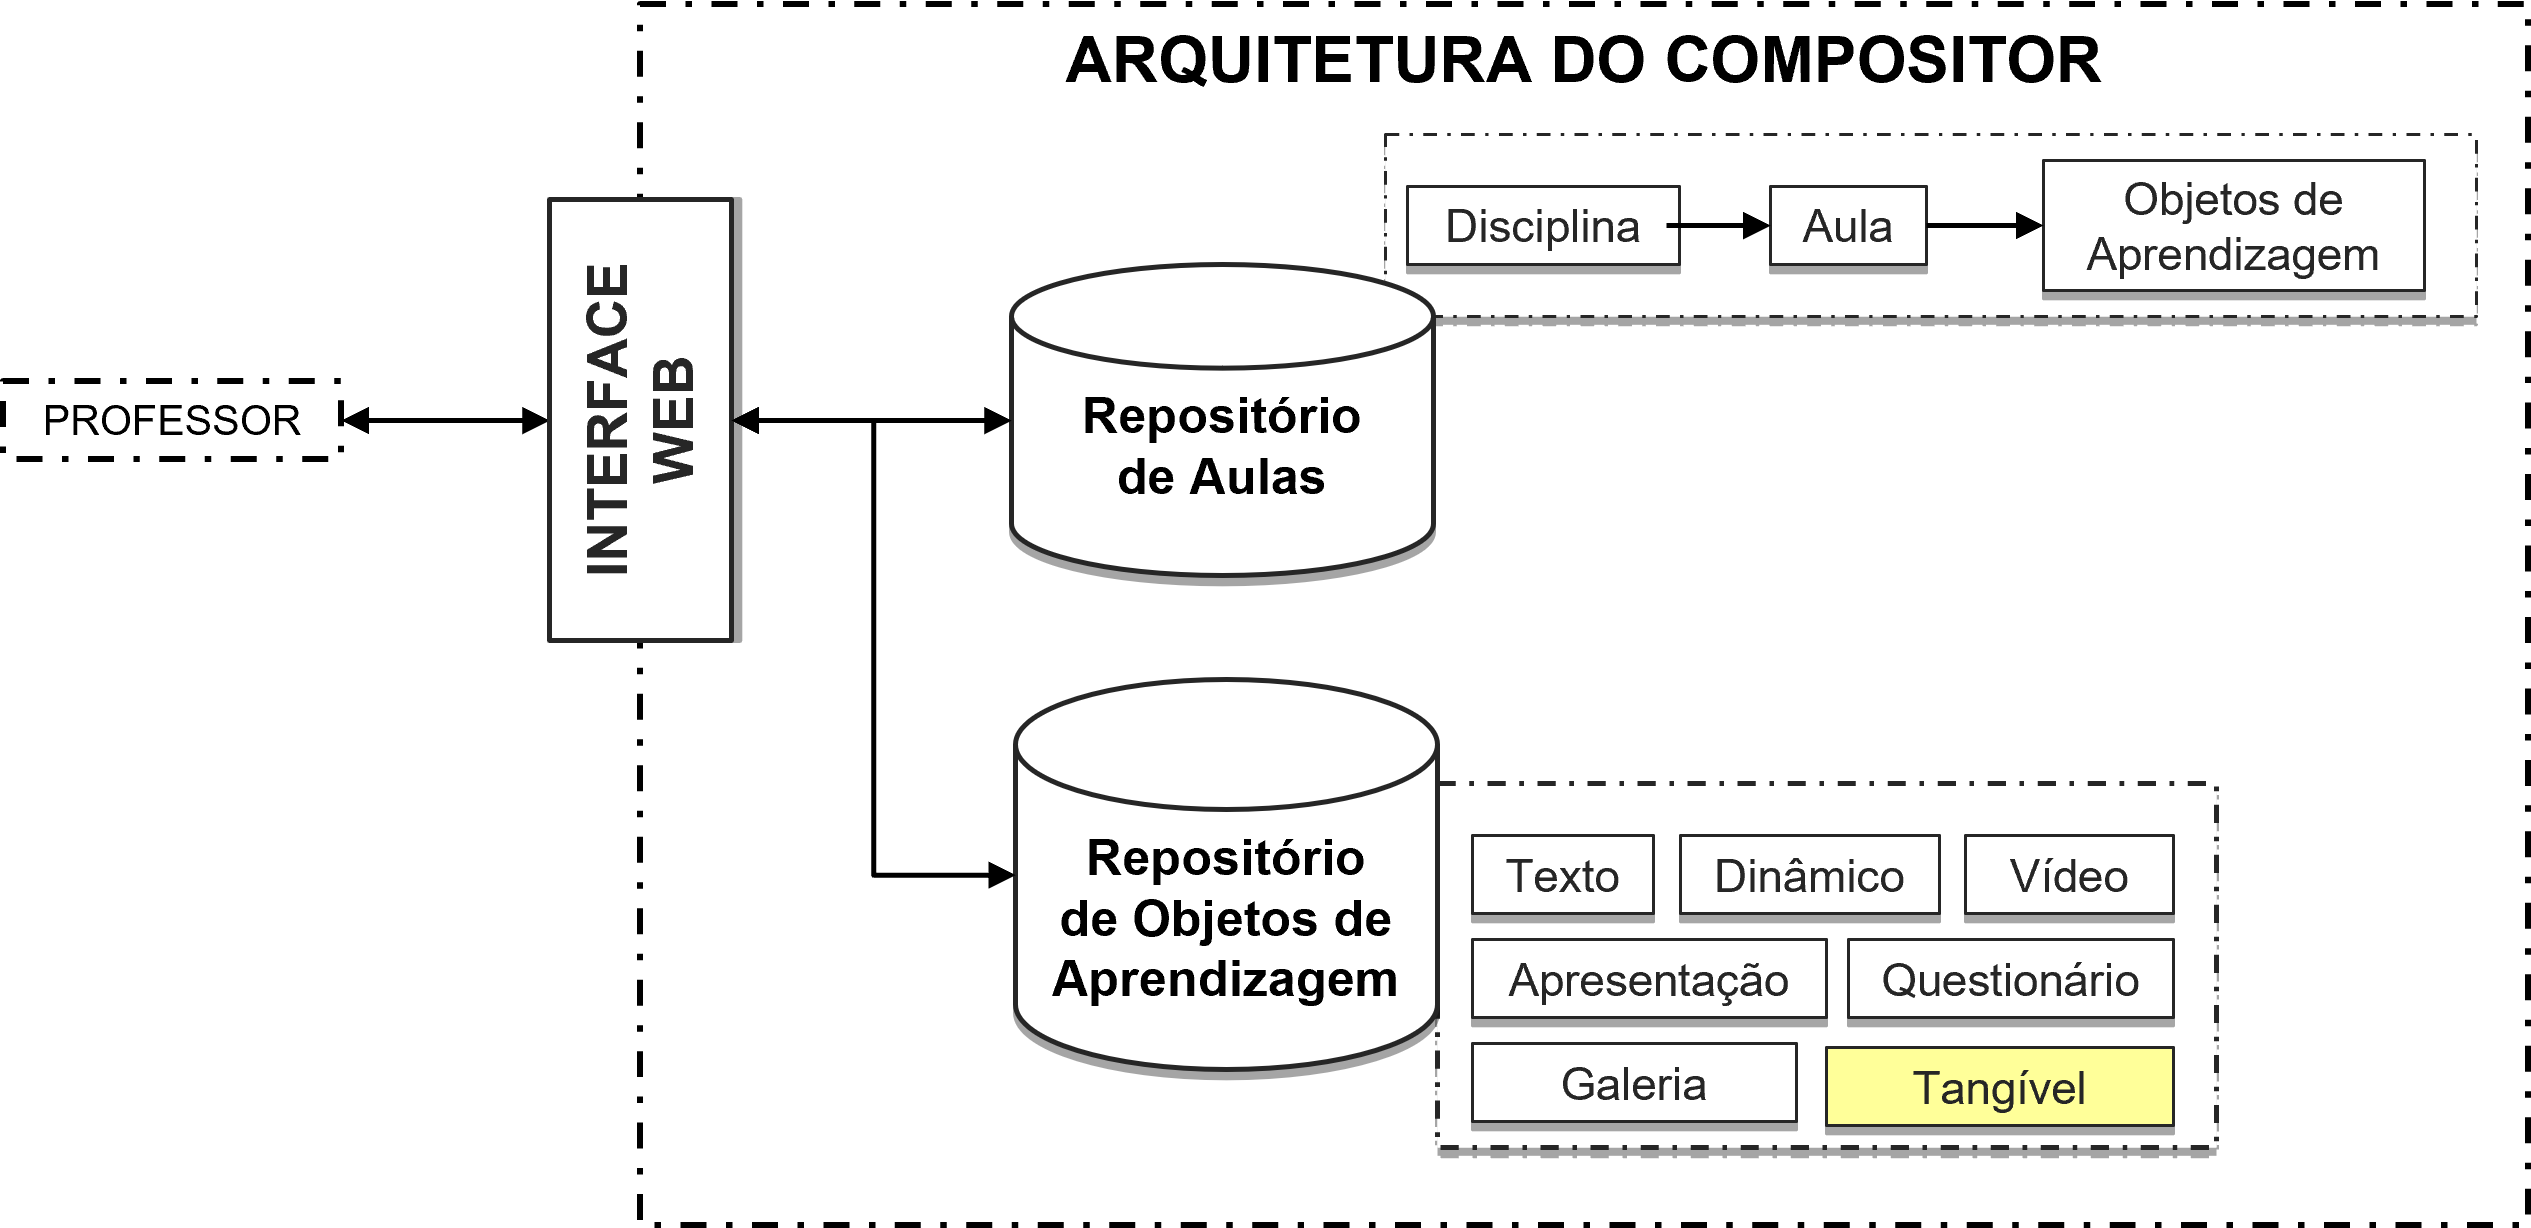
\includegraphics[width=0.9\linewidth]{chapters/proposedMethod/arquitetura_compositor.png}
	\caption{Compositor: arquitetura básica}
	\label{fig:arquitetura_compositor}
\end{figure}

Nesta abordagem, o banco de dados foi modelado para descrever os objetos de aprendizagem de tal modo que os seus metadados sejam compatíveis com os padrões IEEE-LOM e OBAA, tendo sido acrescentadas informações além do padrão relacionadas às métricas de aprendizagem e ao uso dos objetos tangíveis.

Com relação às métricas de aprendizagem (ver Seção~\ref{section:analytics}), considerando inicialmente objetos de aprendizagem do tipo questão de múltipla-escolha, foram acrescentadas informações relativas aos pesos das alternativas a serem escolhidas pelos alunos, além do tempo estimado pelo professor para que os alunos respondam a questão. Além disso, as informações relativas ao nível de dificuldade, previstas pelo IEEE-LOM e que são utilizadas na métrica de Nível de Compreensão, apresentada na Seção~\ref{section:analytics}, foram adaptadas com base no trabalho de~\cite{Biswas:2007}, onde são considerados apenas os níveis `Fácil`, `Normal' e `Difícil'.

% Nesta abordagem, cada Capítulo possui três níveis de dificuldade (`Fácil', `Normal' e `Difícil') previamente definidos pelo professor, quando da criação do mesmo. Além de ter relação com um ou mais capítulos, um objeto de aprendizagem possui um atributo `Conceito' que é o assunto específico tratado pelo objeto. Este atributo tem seu nível de dificuldade baseado nos mesmos três níveis dos Capítulos. Assim, tomando como exemplo, a disciplina de Física do currículo do Ensino Médio, tem-se o \textit{Capítulo} sobre `Oscilações, ondas, óptica e radiação' que tem nível de dificuldade `Difícil', onde é abordado o \textit{Conceito} de `Reflexão e Refração' que tem nível de dificuldade `Normal'.

% Essa classificação dos níveis do \textit{Capítulo} e do \textit{Conceito}, indicada pelo professor, será um elemento a ser levado em consideração nas métricas e análises de aprendizagem propostas neste trabalho. Entretanto, 
Para elaboração de uma aula completa, conceitualmente, o módulo Compositor aceita sete tipos de objetos de aprendizagem: (i) Galeria; (ii) Texto; (iii) Vídeo; (iv) Dinâmico; (v) Apresentação; (vi) Questionário; e, (vii) Tangível (Figura~\ref{fig:arquitetura_compositor}). Dos quais, os seis primeiros foram apresentados na dissertação de mestrado deste proponente~\citep{leitao:2017}.

% %\begin{figure}[h]
% %	\centering
% %	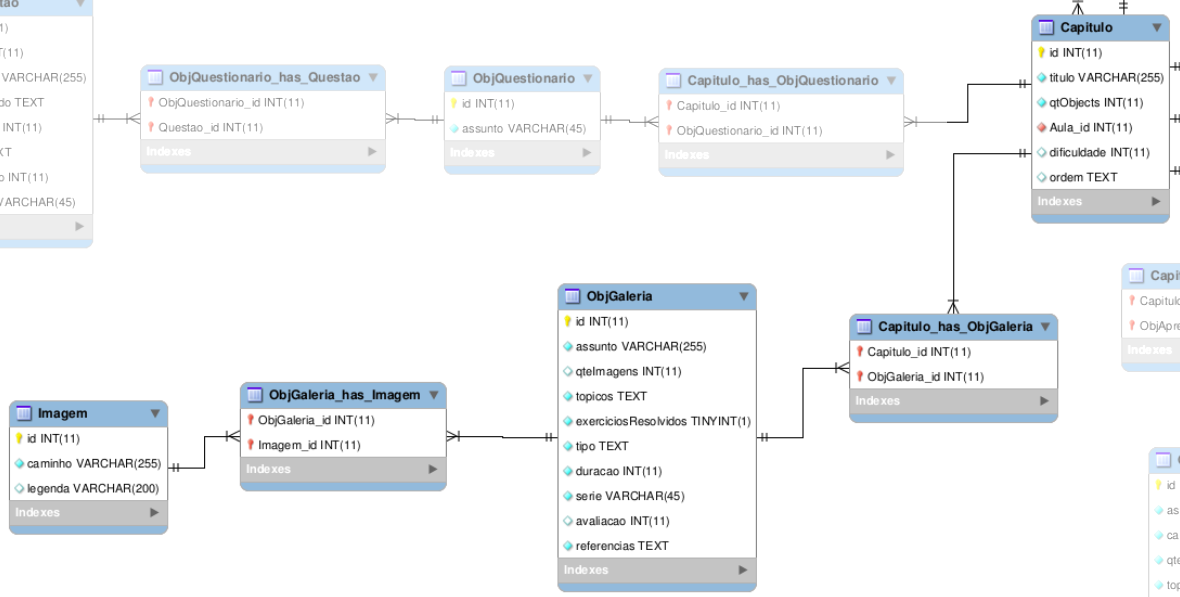
\includegraphics[width=1\linewidth]{imgs/ERComposer_galeriav2}
% %	\caption{Compositor: objetos `Galeria' e `Questionário'}
% %	\label{fig:composergaleria}
% %\end{figure}


Desse modo, o objeto `Galeria' corresponde a uma coleção de imagens, onde cada imagem é um objeto único no banco de dados e pode ser utilizada em diferentes galerias. O objeto `Texto' armazena conteúdos textuais da aula, podendo ser usado para descrição de atividades a serem feitas pela turma ou ainda para simples adição de conteúdos de texto sobre o tema a ser estudado.

O objeto `Vídeo' guarda informações relativas aos vídeos que serão exibidos durante uma aula, enquanto um objeto `Dinâmico' prevê a inserção de objetos com algum nível de interação, tais como \textit{applets} provenientes do Geogebra\footnote{Aplicativo de matemática que combina dinamicamente conceitos de geometria e álgebra em uma única interface do usuário.}. O objeto `Apresentação' corresponde aos \textit{slides} provenientes de ferramentas de escritório, sendo que o compositor converte todos os \textit{slides} em imagens, de modo a possibilitar a obtenção de informações mais precisas sobre a navegação do estudante neste tipo de objeto.

% %\begin{figure}[h]
% %	\centering
% %	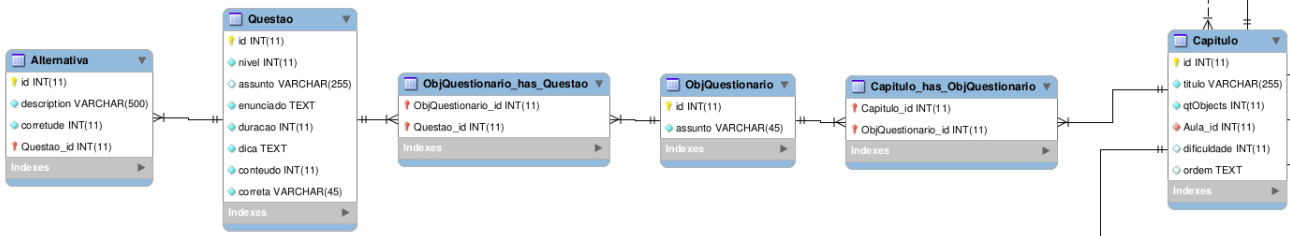
\includegraphics[width=1\linewidth]{imgs/ERComposer_questao}
% %	\caption{Compositor: 'Questionário'}
% %	\label{fig:composerquestionario}
% %\end{figure}

% \begin{figure}[ht]
% 	\centering
% 	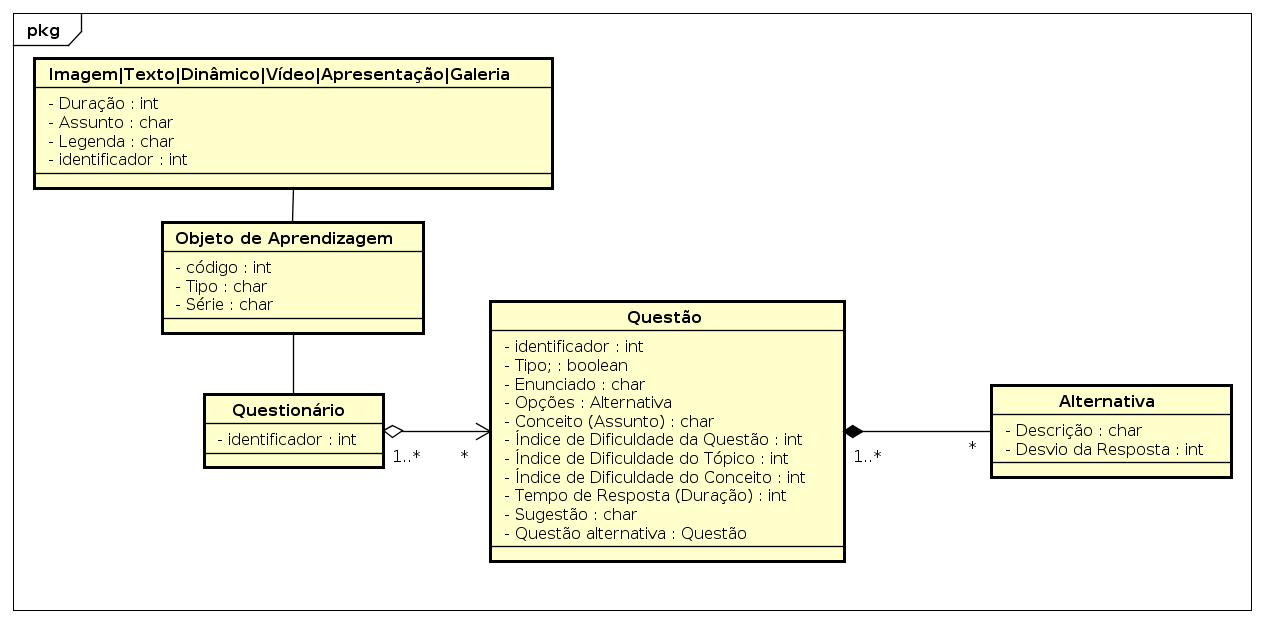
\includegraphics[width=1\linewidth]{imgs/Objetos_de_Aprendizagem}
% 	\caption{Compositor: Modelo dos Objetos de Aprendizagem}
% 	\label{fig:composerquestionario}
% \end{figure}

\textbf{OA Questionário}

O objeto de aprendizagem `Questionário' é uma coleção de questões para verificação do aprendizado do aluno de acordo com as métricas apresentadas na Seção~\ref{section:analytics}. Assim, como o objeto Galeria, cada questão cadastrada é um único objeto de aprendizagem que pode ser reutilizado em outros questionários.
% (Figura~\ref{fig:composerquestionario}). 

Ao criar uma questão, o autor do objeto deve inserir informações relativas ao `Índice de Dificuldade da Questão (IDQ)', `Índice de Dificuldade do Conteúdo (IDC)', `Tempo de Resposta do estudante', que é o tempo máximo esperado que o estudante responda a questão, e ao `Peso' de cada alternativa de resposta da Questão, que tem relação com a proximidade que uma alternativa está da resposta correta, isto é, quanto mais perto da resposta correta, maior o peso. 
%Essa proximidade é medida em cinco níveis, sendo melhor detalhada na Seção~\ref{sec:compreensao-questao}. 
A Figura~\ref{fig:compositor_questao} apresenta uma pré-visualização de um questionário no Compositor, onde é possível conferir esses elementos nos itens adicionados a um questionário.

\begin{figure}[htb]
	\centering
	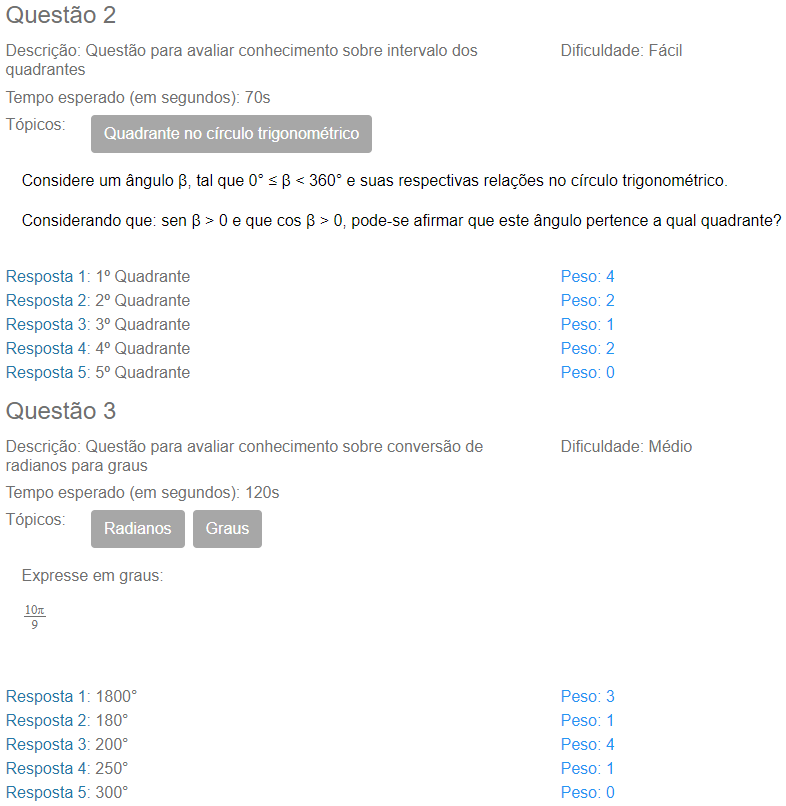
\includegraphics[width=0.9\linewidth]{chapters/proposedMethod/compositor_questoes.png}
	\caption{Compositor: Pré-visualização do Questionário}
	\label{fig:compositor_questao}
\end{figure}

% Além das informações já mencionadas, vale ressaltar que o questionário está inserido no contexto de uma proposta de ajuda sob demanda. Assim, a visualização e os recursos disponíveis, durante a resolução de uma questão, podem ser modificados de acordo com a percepção do sistema da dificuldade do estudante em dar uma resposta ao problema proposto.

% Como parte do mecanismo de modificação na aparência das questões, no momento da criação da questão, o professor precisará introduzir outros três elementos: (i) `Sugestão', que é uma frase ou parágrafo relacionado ao conteúdo que ajude a iluminar o problema; (ii) `Conceito', isto é, o assunto específico da questão, o que possibilitará uma consulta mais rápida e focada ao material didático fornecido; e (iii) `Questão Alternativa' que é uma questão sobre o mesmo assunto e com nível de dificuldade menor ou igual ao da questão principal. Assim, com a \textit{Sugestão} e o \textit{Conceito}, a questão alternativa também servirá como iluminação da resposta da questão principal.

% Na Figura~\ref{fig:composerquestao}, que representa uma questão com os atributos inseridos através do Compositor, pode-se observar tanto dados relacionados às métricas de aprendizagem quanto às opções de ajuda sob demanda.

% \begin{figure}[ht]
% 	\centering
% 	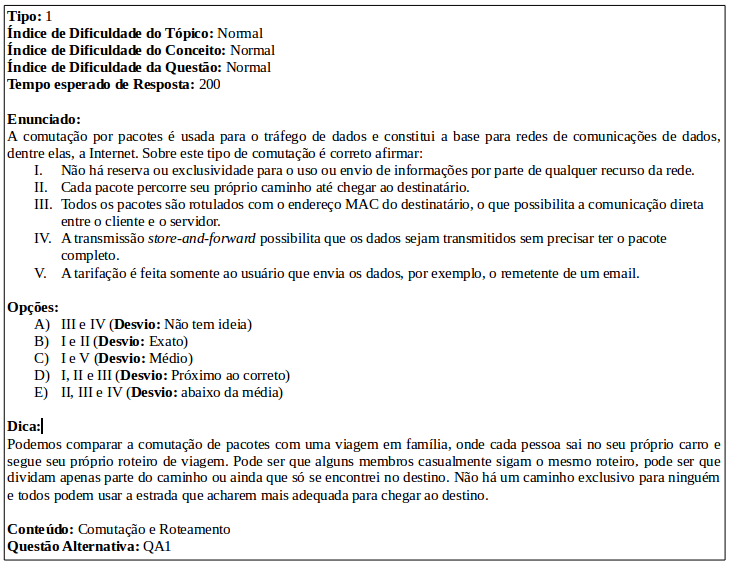
\includegraphics[width=1\linewidth]{imgs/exemplo_questao}
% 	\caption{Compositor: Exemplo de Atributos de uma Questão}
% 	\label{fig:composerquestao}
% \end{figure}

% %\begin{figure}[h]
% %	\centering
% %	\includegraphics[width=1\linewidth]{imgs/composer}
% %	\caption{Exemplo de Tela do Composer}
% %	\label{fig:composer}
% %\end{figure}

% %A Figura~\ref{fig:composer} exibe uma tela com objetos de aprendizagem cadastrados no banco e associados a uma aula de Matemática. Tais objetos serão utilizados para compor o Player e serão utilizados durante a execução da aula presencial.

\textbf{OA Tangível}\label{section:OA_fisicovirtual}

Objetos Tangíveis de Aprendizagem (OTA) são manipulativos que contém, ao mesmo tempo, uma parte física e uma parte digital integradas entre si de modo que, ao ser criado no Compositor, cada OTA precisa ter componentes de ambas as partes devidamente instanciados e suas relações descritas.

Desse modo, será utilizado o conceito de objeto inteligente, apresentado na Seção~\ref{section:iot} e definido por \cite{serbanati:2011}, onde um objeto inteligente tem uma entidade digital e uma entidade física associadas através de um \textit{proxy} digital (vide p.~\pageref{fig:modeloiot}), de modo que o proxy digital atue como uma representação da entidade física no mundo digital. Além disso,~\cite{pires:2015} afirmam que um modelo de entidade virtual precisa ter um identificador unívoco e 
% um tipo (\textit{entityType}), 
atributos com informações sobre a entidade virtual e associação com os serviços que permitem o acesso aos recursos dos dispositivos por parte da entidade.

\begin{figure}[ht]
	\centering
	\includegraphics[width=0.8\linewidth]{chapters/proposedMethod/modelo_OTA.png}
	\caption{Modelo de Objeto Tangível de Aprendizagem proposto neste trabalho}
	\label{fig:modelo_ota}
\end{figure}

%Em vista disso, o modelo referencial de IoT apresentado na Figura~\ref{fig:modeloiot}, onde é definido um objeto inteligente com seus atributos e relações, foi adaptado para o modelo formal de objeto tangível de aprendizagem utilizado neste trabalho, de modo que um OTA contém quatro componentes principais: Dispositivos, \textit{Gateway}, Recursos e Serviços. Assim, Dispositivos são componentes de \textit{hardware} que funcionam como atuadores, TAGs e sensores e são utilizados na instrumentação do objeto, de modo que no contexto deste trabalho a descrição dos recursos é feita através de um código-fonte . Recursos são componentes digitais que fazem referência às propriedades físicas e digitais do objeto, de modo que as informações de ambas as partes possam ser recuperadas ou modificadas, assim, nesta proposta, a descrição dos Recursos corresponde a definição das variáveis de entrada e saída físicas e virtuais.
Em vista disso, o modelo referencial de IoT apresentado por \cite{serbanati:2011} que define um objeto inteligente, seus atributos e relações foi adaptado conforme apresentado na Figura~\ref{fig:modelo_ota}, e servirá de modelo para o objeto tangível de aprendizagem utilizado neste trabalho, de modo que um objeto tangível de aprendizagem proposto nestes termos contém quatro componentes principais: Dispositivos, \textit{Gateway}, Recursos e Serviços. 

Assim, Dispositivos são os componentes de \textit{hardware} que funcionam como atuadores, TAGs e sensores e são utilizados na instrumentação do objeto de aprendizagem. O Gateway é um componente que garante o acesso aos Dispositivos e deve ser executado em um microcontrolador com capacidade de transmissão e recepção de pacotes de mensagens, de modo que a comunicação entre as entidades física e a virtual do objeto seja estabelecida através de um protocolo de troca de mensagens.

Recursos são componentes digitais que fazem referência às propriedades físicas e digitais do objeto, de modo que as informações de ambas as partes possam ser recuperadas ou modificadas. Assim, nesta proposta, a descrição dos Recursos corresponde a definição das variáveis de entrada e saída físicas e virtuais.

\begin{figure}[htb]
	\centering
	\includegraphics[width=1\linewidth]{chapters/proposedMethod/bpmn_ofva.png}
	\caption{Modelo BPMN para Criação de OTAs vinculados a uma plataforma educacional}
	\label{fig:bpmn_ofva}
\end{figure}

Além disso, é preciso que o compositor de objetos de aprendizagem seja capaz de integrar um manipulativo físico, instrumentado com sensores diversos, a um conjunto de páginas web que implementam um manipulativo virtual, com entradas e saídas equivalentes ao físico, de modo que o produto do processo seja um objeto com ambos os manipulativos físico e virtual integrados como um único objeto físico/digital de aprendizagem. Assim, o componente Serviços descreve e implementa as ações que estarão disponíveis ao usuário no Player (ver Seção~\ref{section:player}) e que garantem ao estudante o acesso aos Recursos do OTA, de modo que são especificados tanto os componentes necessários a execução da entidade digital associada ao objeto físico (páginas web, componentes javascript) quanto quais entradas e saídas físicas e digitais serão utilizadas em cada caso de teste com suas respectivas regras de avaliação da aprendizagem e \textit{feedback}, conforme o necessário (Figura~\ref{fig:bpmn_ofva_casos}).

\begin{figure}[htb]
	\centering
	\includegraphics[width=0.9\linewidth]{chapters/proposedMethod/bpmn_servicos.png}
	\caption{Subprocesso `Definir Serviços'}
	\label{fig:bpmn_ofva_casos}
\end{figure}

É importante salientar que, no contexto deste trabalho, um caso de teste equivale uma situação-problema que pode ser instrumentada com parâmetros (regras) que permitam ao Player auxiliar o estudante no caminho de construção do conhecimento, de modo que ele possa corrigir as suas respostas até que descubra a resposta correta ao utilizar o objeto tangível no \textbf{modo estudo}. Além disso, para que o objeto tangível seja utilizado para o acompanhamento/avaliação da aprendizagem, um caso de teste também precisa estar associado aos parâmetros das diversas métricas propostas neste trabalho (Seção~\ref{section:analytics}).

%Além disso, para que o fluxo desse processo aconteça conforme o necessário, é preciso que o compositor de objetos de aprendizagem seja capaz de integrar um manipulativo físico instrumentado com sensores diversos a um conjunto de páginas web que implementam um manipulativo virtual com entradas e saídas equivalentes ao físico, de modo que o produto do processo seja um objeto com ambos os manipulativos físico e virtual integrados como um único objeto físico-virtual de aprendizagem.

A fim de formalizar esta proposta, diagramas de processos BPMN (\textit{Business Process Model and Notation}) foram definidos de modo a orientar os passos para composição de um OTA. Assim, as Figuras \ref{fig:bpmn_ofva} e \ref{fig:bpmn_ofva_casos} apresentam o modelo, onde o autor dos objetos de aprendizagem precisa definir: (i) aspectos educacionais do OTA; (ii) gateway; (iii) dispositivos (hardware); (iv) recursos (entradas e saídas físicas e virtuais) e (v) serviços (componentes digitais e casos de teste). A Tabela~\ref{tabela:OFV} detalha os atributos necessários para a construção de um objeto tangível de aprendizagem conforme o modelo proposto.

% Entretanto, para a formalização da instanciação dos elementos dos OFV e facilitar a comunicação entre os componentes da plataforma deverá ser definida uma linguagem de marcação que consiga descrever os atributos e dados coletados de cada objeto físico-virtual de aprendizagem. Dentre as opções de linguagens estão a OWL e a EEML que são muito utilizadas para essa finalidade, estando presentes em quase todas os \textit{middleware} IoT apresentados por~\cite{pires:2015}. Em vista das limitações inerentes a estas linguagens, deverá ser feita uma extensão dos seus elementos para que possibilitem uma descrição mais adequada dos dados coletados provenientes dos diversos sensores ou atuadores.


\begin{table}[htb]
\caption{Atributos de um Objeto Tangível de Aprendizagem}
\centering

\begin{tabularx}{\textwidth}{|c|X|}
\hline
\textbf{Atributo} & \textbf{Descrição} \\ \hline
\textbf{ID} & Identificador unívoco do OTA \\ \hline
\textbf{Título} & Nome do OTA \\ \hline
\textbf{Descrição Geral} & Descrição textual acerca do conteúdo do OTA \\ \hline
\textbf{Descrição Educacional} & Descrição acerca de como o OTA deve ser usado \\ \hline
\textbf{Tópicos} & Conceitos abordados pelo OTA \\ \hline
\textbf{Modo} & -\textbf{Estudo}: modo com \textit{feedbacks} em tempo de interação do aluno com dicas sobre o tópico estudado e a posteriori das métricas de aprendizagem;

	-\textbf{Avaliação}: modo apenas com \textit{feedback} a posteriori das métricas de aprendizagem\\ \hline
\textbf{Gateway} & Código-fonte a ser executado em um microcontrolador\\ \hline
\textbf{Dispositivos} & Sensores, tags ou atuadores que compõem o OTA\\ \hline
\textbf{Recursos} & Conjuntos de Entradas e Saídas Físicas e Digitais com rótulos, tipos de dado e valores\\ \hline
\textbf{Serviços} &  -\textbf{Componentes Digitais} da Entidade Virtual (páginas web, javascripts,...); 

-\textbf{Casos de Teste}: Situações-problema a serem resolvidas pelos estudantes com fins de acompanhamento/verificação da aprendizagem. É necessário indicar os parâmetros das métricas de avaliação propostas neste trabalho (níveis de dificuldade, pesos, tempo...). \\ \hline
\end{tabularx}
\label{tabela:OFV}
\end{table}

Adicionalmente, o Compositor de OTA utiliza uma linguagem de programação em blocos baseada na biblioteca Blockly~\citep{Blockly:2022} para definição das Entradas e Saídas e das regras dos Casos de Teste (Figura~\ref{fig:blockly_exemplo}). Tais elementos serão utilizados pela plataforma para comunicação e respostas do servidor às ações dos estudantes na parte virtual, inclusive com relação às respostas esperadas para as situações-problema definidas pelo autor do objeto de aprendizagem, uma vez que Blockly permite a tradução da lógica dos blocos para outras linguagens de programação como JavaScript (Figura~\ref{fig:blockly_exemplo}), PHP e Python.

\begin{figure}[ht]
	\centering
	\includegraphics[width=1\linewidth]{chapters/proposedMethod/Blockly.png}
	\caption{Exemplo de definição de regra para caso de teste e sua tradução para linguagem JavaScript}
	\label{fig:blockly_exemplo}
\end{figure}


Além disso, é importante ressaltar que, ao desafio de modelar e padronizar os objetos tangíveis de aprendizagem, acrescentam-se: (i) a demanda por uma descrição adequada dos seus metadados de modo a facilitar não apenas a criação de repositórios, mas, a recomendação e o reuso desses tipos de objetos; e, (ii) a necessidade de estabelecer critérios de avaliação e verificação do aprendizado de maneira automática.

\textbf{Padrão de Metadados}

Com relação a descrição dos metadados, após estudar alguns dos padrões existentes como Dublin Core, IEEE-LOM e OBAA, optou-se pelo último, que é derivado do padrão IEEE-LOM. Essa opção foi feita pelo fato do OBAA ser um padrão brasileiro presente implementado em importantes repositórios de objetos de aprendizagem nacionais, além de oferecer suporte a mídias de diferentes plataformas, dentre elas, TV Digital, Web e Móveis, ter descritores educacionais com uma base epistemológica interacionista e descritores de acessibilidade~\citep{vicari:2009}.

Assim, inicialmente, foi escolhido o perfil compatível ideal com o OBAA denominado ``PM-OBAA-FULL''. Entretanto, para melhor descrição dos objetos de aprendizagem que estamos usando, alguns dos descritores fora do perfil ideal padrão foram utilizados. A tabela do Apêndice~\ref{Chap:AppendixA} apresenta os descritores atualmente utilizados. 

%\textbf{ATUALIZAR TEXTO A SEGUIR: Além disso, nos próximos passos, a pesquisa será aprofundada com vistas a propor uma extensão do padrão OBAA que descreva adequadamente objetos físico-virtuais de aprendizagem.}

\section{Servidor}\label{section:service}
É o módulo que cria uma sala de aula virtual, gerencia as trocas de mensagens entre os dispositivos dos estudantes e do professor, além de consolidar os dados para análise de acordo com as métricas de aprendizagem propostas. Com a adição dos objetos tangíveis de aprendizagem, o Servidor também tratará os dados provenientes da interação dos estudantes com ambas as partes física e digital do objeto, além de disponibilizar acesso aos recursos virtuais do OTA.

% além de realizar modificações na apresentação das questões, segundo uma abordagem de percepção da dificuldade dos estudantes.

\begin{figure}[htbp]
	\centering
	\includegraphics[width=0.8\linewidth]{chapters/proposedMethod/arquitetura_servidor.png}
	\caption{Arquitetura do Servidor}
	\label{fig:servidor}
\end{figure}

Inicialmente, o professor disponibiliza através do Servidor a aula a ser ministrada juntamente com as informações da turma que terá aula (por exemplo: nome, matrícula, senha,...). Esse carregamento é necessário pois, por decisão de projeto, a plataforma foi implementada de modo a levar em consideração que o acesso a internet em escolas periféricas brasileiras pode ser restrito ou inexistente e, no caso amazônico, essas escolas também podem estar situadas em municípios interioranos ou comunidades ribeirinhas. Dessa forma, o protótipo de servidor que gerencia a aula contendo o objeto tangível implementado neste trabalho provê a condução da aula sem uma conexão com a internet.

Após o carregamento da aula e das turmas relacionadas, uma sessão é criada para cada aluno que se conecta ao Servidor e, além disso, o conteúdo da aula é disponibilizado via \textit{streaming} para cada dispositivo conectado de acordo com as requisições HTTP Rest executadas. Desse modo, o Servidor terá uma tripla finalidade: (i) gerenciar as conexões dos alunos com a finalidade de coletar dados e armazenar \textit{logs} de interação dos estudantes com o material didático; (ii) prover acesso às possíveis notificações e recomendações pedagógicas; e, (iii) prover acesso aos recursos dos objetos de aprendizagem.
% e, de acordo com as dificuldades apresentadas pelos alunos na hora de responder um questionário avaliativo, apresentar recursos adicionais de ajuda. 

A Figura~\ref{fig:servidor} destaca em amarelo as modificações feitas na estrutura do servidor em relação ao proposto originalmente por~\cite{leitao:2017}, em especial os acréscimos necessários para que o mesmo trabalhe com objetos tangíveis de aprendizagem. Desse modo, podemos observar um novo componente correspondente aos  ``Recursos'', que é responsável por referenciar as entradas e saídas físicas e digitais do objeto com o objetivo de armazenar essas interações no log. O segundo componente adicionado corresponde aos ``Serviços'' disponibilizados pelo Player e que estão armazenados no banco de dados, tais serviços correspondem ao conteúdo dos objetos (ie: páginas web, códigos em javascript que proveem o \textit{feedback} do modo estudo).

Por fim, pode-se notar que a comunicação com os módulos Analytics, o novo Player Tangível e os repositórios de objetos de aprendizagem e de aulas acontece via HTTP Rest.

\section{Player Tangível}\label{section:player}
% %É um conjunto de páginas web contendo todo o material didático de uma aula a ser ministrada (Figura~\ref{fig:aulaplayer}). Tais páginas são executadas em um navegador de internet, onde acontece a interação do estudante com o material didático.

% %\begin{figure}[h]
% %\centering
% %\includegraphics[width=0.75\linewidth]{imgs/player_aulageometria}
% %\caption{Exemplo de aula sendo executada no Player}
% %\label{fig:aulaplayer}
% %\end{figure}

O Player apresentado por~\cite{leitao:2017}, é definido como um conjunto de páginas web contendo todo o material didático de uma aula a ser ministrada, de modo que tais páginas são executadas em um navegador de internet, através do qual acontece a interação do estudante com o conteúdo educacional. O Player Tangível expande esse conceito de modo que o novo \textit{player} conta com uma interface física (manipulativo físico instrumentado com sensores) cuja interação do aluno reflete na sua respectiva interface digital.

Assim, enquanto o Player tradicional possui duas partes principais (Figura~\ref{fig:arquiteturaplayer}): (i) Aula Digital; (ii) Coletor de Dados; onde, a `Aula Digital' é o material didático baseado em web e o `Coletor de Dados' é um rastreador que coleta os cliques dos alunos. O conceito de Player Tangível acrescenta uma terceira parte relacionada a `entidade física' que é integrada a sua respectiva contraparte `entidade digital' através do \textit{Gateway}. 

Assim, o que para \cite{leitao:2017} corresponde a aula digital provendo os diversos objetos de aprendizagem tradicionais (questionários, slides, vídeos,...), neste trabalho, o mesmo componente provê também a entidade digital do objeto tangível, correspondendo assim ao \textit{proxy digital} do objeto físico/digital. Ademais, na entidade física, pode-se notar a presença dos componentes `Dispositivos', `Gateway' e `Recursos' definidos no modelo proposto de um objeto tangível (Figura~\ref{fig:modelo_ota}) conforme a proposta deste trabalho. O componente `Serviços' serve de ponte para ambas as interfaces física e digital de modo que as entradas físicas e digitais correspondentes e o conteúdo educacional sejam acessados pelos estudantes.

%de `controle de objeto' atrelada aos `atributos' deste objeto (entradas físicas e virtuais e regras dos casos de teste) de modo a proporcionar a comunicação em tempo real entre as partes física e virtual, de modo que toda manipulação física do aluno é refletida automaticamente na sua parte virtual.

% É essa interação do Coletor com o Servidor que viabilizará os três níveis de ajuda sob demanda apresentados nas Seções~\ref{section:composer} e \ref{section:service}.

\begin{figure}[htb]
	\centering
	\includegraphics[width=1\linewidth]{chapters/proposedMethod/arquitetura_player.png}
	\caption{Arquitetura do Player Tangível}
	\label{fig:arquiteturaplayer}
\end{figure}

Assim, a proposta de Player Tangível apresentada neste trabalho conta com duas interfaces de comunicação com o usuário (professores ou estudantes), uma baseada em web e outra baseada em manipulativo físico. A interface digital permite a entrega do conteúdo educacional digital em praticamente qualquer dispositivo e plataforma sem necessidade de instalação de \textit{softwares} adicionais. Essa característica possibilita grande portabilidade dessa parte do sistema e, por conseguinte, baixo custo de implantação, visto que cada aluno pode, por exemplo, usar seu próprio dispositivo móvel durante a aula. Essa abordagem visa não apenas inserir definitivamente as novas tecnologias em sala de aula, mas, tirar proveito dos recursos que os estudantes trazem consigo, além de tentar aumentar o nível de engajamento do estudante em uma aula.

Por fim, é importante notar que a interface física está atrelada ao manipulativo físico utilizado, o qual deve possuir um conjunto de dados que o descrevam, incluindo informações acerca dos sensores utilizados, dos formatos de dados e das ações executadas como resposta às interações dos estudantes (conforme especificado nas regras dos casos de teste). Assim como os outros objetos de aprendizagem, os OTA também tem seus dados de interação coletados pelo sistema com a finalidade de viabilizar uma análise inteligente da aprendizagem que permita extrair conhecimentos sobre o comportamento e o desempenho dos estudantes para, no futuro, propor recursos ou estratégias educacionais que colaborem efetivamente na melhoria da aprendizagem.

%Dentre os dados a serem descritos, além dos necessários ao funcionamento do OTA que devem ser descritos em alguma linguagem que permita a associação com sensores tais como OWL ou EEML, é importante ressaltar a necessidade de se estender algum padrão de metadados de modo a descrever adequadamente estes objetos.

\subsection{Processo de conexão entre as entidades física e digital}\label{sub:JSON}

Em termos de ferramenta, propomos a utilização do protocolo \textit{Websocket} de modo a tornar a comunicação em tempo real mais eficiente, onde o \textit{Gateway} apresentado no Modelo de Referência (Figura~\ref{fig:modelo_ota}) como elemento de integração entre as entidades física e digital foi implementado, nesta proposta de Tese, como um servidor \textit{Websocket} (ver Subseção~\ref{subsec:tools_player}). 

Além disso, como parte da formalização desta proposta, para o processo de troca de mensagens com o Gateway, foi escolhido o formato \textit{JSON} de modo a garantir que maior compatibilidade entre as partes física e digital, de modo que a Tabela~\ref{tabela:JSON} apresenta uma descrição inicial dos principais campos utilizados no formato definido, que serão detalhados no decorrer desta seção.

% Please add the following required packages to your document preamble:
% \usepackage[table,xcdraw]{xcolor}
% If you use beamer only pass "xcolor=table" option, i.e. \documentclass[xcolor=table]{beamer}
\begin{table}[htb]
	\caption{Campos para troca de mensagens entre as entidades do Player Tangível}
	\centering
	\begin{tabular}{|c|c|c|c|}
		\hline
		\rowcolor[HTML]{C0C0C0} 
		\textbf{Campo} & \textbf{Tipo} & \textbf{Descrição} & \textbf{Observação} \\ \hline
		type & string & Tipo da mensagem & Obrigatório \\ \hline
		action & string & Ação a ser realizada & Obrigatório \\ \hline
		data & object & Informação específica de cada mensagem & Opcional \\ \hline
		error & object & Detalhes do erro & Opcional \\ \hline
	\end{tabular}
	\label{tabela:JSON}
\end{table}

A Listagem~\ref{JSON_exemplo} apresenta um exemplo inicial de modelo para o formato JSON a ser utilizado nas mensagens trocadas, note-se que alguns dos campos possuem subcampos que especificam mais informações.

\begin{listing}[htb]
	\begin{minted}[frame=lines,framesep=2mm,fontsize=\footnotesize,linenos]{json}
		{
			"type": "connection",
			"action": "connect",
			"data": {
				"connected": false,
			},
			"error": {
				"code": 1,
				"message": "Já existe um usuário conectado"
			}
		}
	\end{minted}
	\caption{Exemplo de mensagem JSON}
	\label{JSON_exemplo}
\end{listing}

\textbf{Conexão via \textit{Websocket} e preparação para pareamento}

O passo inicial para o pareamento entre as entidades física e virtual é o estabelecimento de uma conexão via \textit{websocket}, por onde todas as mensagens no formato JSON serão trocadas. Assim, a Figura~\ref{fig:diagrama-websockets} apresenta o diagrama de sequência que ilustra esse processo, onde pode-se notar que, após o estudante inserir o número identificador único da entidade física (URI) na parte virtual do Player Tangível, as mensagens seguintes estabelecem primeiro um canal \textit{websocket} e, em seguida, é feita uma primeira troca de mensagens para verificação da possibilidade de pareamento entre as entidades.

\begin{figure}[htb]
	\centering
	\includegraphics[width=0.9\linewidth]{chapters/proposedMethod/msg_websocket.png}
	\caption{Diagrama de Sequência - Conexão Websocket}
	\label{fig:diagrama-websockets}
\end{figure}

%A Tabela~\ref{tab:websocket} detalha a mensagens que devem ser trocadas durante esta etapa prévia ao pareamento. 
É importante notar que após a confirmação do \textit{handshake}, a interface virtual envia automaticamente a mensagem $M1$ de solicitação de pareamento (Tabela~\ref{tab:websocket}), obtendo como resposta a mensagem $M2$, que pode ser tanto de confirmação quanto de recusa da solicitação. 

\begin{table}[htb]
	\centering
	\caption{Mensagem de solicitação de pareamento}
	\begin{tabular}{|c|ccc|}
		\hline
		\rowcolor[HTML]{C0C0C0} 
		\textbf{Mensagem} & \multicolumn{3}{c|}{\cellcolor[HTML]{C0C0C0}\textbf{Descrição}} \\ \hline
		M1 & \multicolumn{3}{c|}{Solicitar pareamento} \\ \hline
		\rowcolor[HTML]{C0C0C0} 
		\textbf{Campo} & \multicolumn{1}{c|}{\cellcolor[HTML]{C0C0C0}\textbf{Tipo}} & \multicolumn{1}{c|}{\cellcolor[HTML]{C0C0C0}\textbf{Valor}} & \textbf{Observação} \\ \hline
		\textit{type} & \multicolumn{1}{c|}{\textit{string}} & \multicolumn{1}{c|}{\textit{connection}} & \multicolumn{1}{l|}{} \\ \hline
		\textit{action} & \multicolumn{1}{c|}{\textit{string}} & \multicolumn{1}{c|}{\textit{connect}} & \multicolumn{1}{l|}{} \\ \hline
	\end{tabular}
	\label{tab:websocket}
\end{table}

Uma mensagem de confirmação permite o prosseguimento do processo de pareamento, de modo que a interface física gera um número de \textit{token} que deve ser informado em até 30 segundos através da interface virtual.

\begin{table}[htb]
	\centering
	\caption{Mensagens de solicitação e de status da solicitação de pareamento}
\begin{tabular}{|c|ccc|}
	\hline
	\rowcolor[HTML]{C0C0C0} 
	\textbf{Mensagem} & \multicolumn{3}{c|}{\cellcolor[HTML]{C0C0C0}\textbf{Descrição}} \\ \hline
	M2 & \multicolumn{3}{c|}{Status da solicitação} \\ \hline
	\rowcolor[HTML]{C0C0C0} 
	\textbf{Campo} & \multicolumn{1}{c|}{\cellcolor[HTML]{C0C0C0}\textbf{Tipo}} & \multicolumn{1}{c|}{\cellcolor[HTML]{C0C0C0}\textbf{Valor}} & \textbf{Observação} \\ \hline
	\textit{type} & \multicolumn{1}{c|}{\textit{string}} & \multicolumn{1}{c|}{\textit{connection}} &  \\ \hline
	\textit{action} & \multicolumn{1}{c|}{\textit{string}} & \multicolumn{1}{c|}{\textit{connect}} &  \\ \hline
	\textit{data.connected} & \multicolumn{1}{c|}{\textit{boolean}} & \multicolumn{1}{c|}{\textit{true | false}} & \begin{tabular}[c]{@{}c@{}}Solicitação recebida com\\ sucesso | Erro no \\pareamento\end{tabular} \\ \hline
	\textit{data.expires\_in} & \multicolumn{1}{c|}{\textit{integer}} & \multicolumn{1}{c|}{30} & \begin{tabular}[c]{@{}c@{}}Tempo de espera para \\ recebimento do Token\end{tabular} \\ \hline
	\textit{error.code} & \multicolumn{1}{c|}{\textit{integer}} & \multicolumn{1}{c|}{1} &  \\ \hline
	\textit{error.message} & \multicolumn{1}{c|}{string} & \multicolumn{1}{c|}{Já existe um usuário conectado} & \begin{tabular}[c]{@{}c@{}}Só é permitida uma conexão \\ por dispositivo físico\end{tabular} \\ \hline
\end{tabular}
	\label{tab:websocketstatus}
\end{table}

Já uma mensagem de recusa de pareamento por parte da entidade física encerra o processo com o código de erro `1' e a mensagem `Já existe um usuário conectado', uma vez que uma entidade física só pode se conectar a uma única entidade virtual.

\textbf{Mensagens relativas ao pareamento}

Quando a interface virtual recebe um \textit{status} de confirmação da solicitação ($M2$ é verdadeiro), então, o usuário tem trinta segundos para inserir na interface virtual e enviar o \textit{token} aleatório que aparece na tela da interface física. Assim, a validação do \textit{token} é solicitada através da mensagem $M3$, que é enviada pela interface virtual para a parte física (vide Figura~\ref{fig:diagrama-token} e Tabela~\ref{tab:tokenM3}).

\begin{figure}[htb]
	\centering
	\includegraphics[width=0.9\linewidth]{chapters/proposedMethod/msg_token.png}
	\caption{Diagrama de Sequência para Pareamento}
	\label{fig:diagrama-token}
\end{figure}

A mensagem $M4$ ocorre quando a entidade física retorna o status do pareamento para a entidade virtual. Essa mensagem pode ser de confirmação (\textit{true}) ou de recusa de pareamento (\textit{false}), conforme ilustrado na Figura~\ref{fig:diagrama-token}. Em caso de confirmação, o status do token para o usuário é dado pela atualização da interface virtual de modo que a entidade virtual se torna visível e passa a exibir a mesma aparência e posição dos elementos da entidade física.

\begin{table}[htb]
	\centering
	\caption{Solicitação de validação do \textit{token}}
	\begin{tabular}{|c|ccc|}
		\hline
		\rowcolor[HTML]{C0C0C0} 
		\textbf{Mensagem} & \multicolumn{3}{c|}{\cellcolor[HTML]{C0C0C0}\textbf{Descrição}} \\ \hline
		M3 & \multicolumn{3}{c|}{Envia Token para validação} \\ \hline
		\rowcolor[HTML]{C0C0C0} 
		\textbf{Campo} & \multicolumn{1}{c|}{\cellcolor[HTML]{C0C0C0}\textbf{Tipo}} & \multicolumn{1}{c|}{\cellcolor[HTML]{C0C0C0}\textbf{Valor}} & \textbf{Observação} \\ \hline
		\textit{type} & \multicolumn{1}{c|}{\textit{string}} & \multicolumn{1}{c|}{\textit{connection}} &  \\ \hline
		\textit{action} & \multicolumn{1}{c|}{\textit{string}} & \multicolumn{1}{c|}{\textit{token}} &  \\ \hline
		data.token & \multicolumn{1}{c|}{string} & \multicolumn{1}{c|}{Token informado pelo usuário} &  \\ \hline
	\end{tabular}
	\label{tab:tokenM3}	
\end{table}

Caso ocorra recusa no pareamento por parte da entidade física, a mensagem $M4$ retorna um dos erros especificados na Tabela~\ref{tab:tokenM4}. De modo que, o erro `2' corresponde a mensagem de que o token informado é inválido por não ser igual ao token mostrado na tela da entidade física e, o erro `3' é relativo ao fato de que o tempo de validade do token expirou. Para o segundo caso, é gerado um novo token com um novo tempo de validade.

\begin{table}[htb]
	\centering
	\caption{Mensagem para validação do \textit{token}}
	\begin{tabular}{|c|ccc|}
		\hline
		\rowcolor[HTML]{C0C0C0} 
		\textbf{Mensagem} & \multicolumn{1}{c|}{\cellcolor[HTML]{C0C0C0}\textbf{Descrição}} & \multicolumn{1}{c|}{\cellcolor[HTML]{C0C0C0}\textbf{}} & \textbf{} \\ \hline
		M4 & \multicolumn{3}{c|}{Status do pareamento} \\ \hline
		\rowcolor[HTML]{C0C0C0} 
		\textbf{Campo} & \multicolumn{1}{c|}{\cellcolor[HTML]{C0C0C0}\textbf{Tipo}} & \multicolumn{1}{c|}{\cellcolor[HTML]{C0C0C0}\textbf{Valor}} & \textbf{Observação} \\ \hline
		\textit{type} & \multicolumn{1}{c|}{\textit{string}} & \multicolumn{1}{c|}{\textit{connection}} & \multicolumn{1}{l|}{} \\ \hline
		\textit{action} & \multicolumn{1}{c|}{\textit{string}} & \multicolumn{1}{c|}{\textit{token}} & \multicolumn{1}{l|}{} \\ \hline
		\textit{data.is\_valid\_token} & \multicolumn{1}{c|}{\textit{boolean}} & \multicolumn{1}{c|}{\textit{true | false}} & \multicolumn{1}{l|}{\begin{tabular}[c]{@{}l@{}}True: Token é válido. \\ False: Token informado é \\ inválido ou o tempo de \\ validação expirou (erro é\\ detalhado)\end{tabular}} \\ \hline
		\textit{error.code} & \multicolumn{1}{c|}{\textit{integer}} & \multicolumn{1}{c|}{2 | 3} & \multicolumn{1}{l|}{\begin{tabular}[c]{@{}l@{}}2: Token inválido\\ 3: Token expirado\end{tabular}} \\ \hline
		\textit{error.message} & \multicolumn{1}{c|}{string} & \multicolumn{1}{c|}{\begin{tabular}[c]{@{}c@{}}2:Token inválido\\ 3: Token expirado\end{tabular}} & \multicolumn{1}{l|}{\begin{tabular}[c]{@{}l@{}}2: O token enviado pelo \\ virtual não coincide com \\ o gerado pelo físico.\\ 3: O tempo para validação\\ do token expirou. É \\ necessário gerar um novo.\end{tabular}} \\ \hline
	\end{tabular}
	\label{tab:tokenM4}	
\end{table}


\textbf{Envio de Dados}

Com o estabelecimento da conexão entre as entidades física e virtual, qualquer manipulação captada pelos sensores presentes no artefato físico deve refletir na sua respectiva contraparte virtual, de modo que, a partir deste momento, todas as mensagens enviadas da parte física para a virtual são relativas a atualização das posições do manipulativo físico e correspondem às entradas físicas definidas no projeto do objeto tangível, de modo que a mensagem $M5$ é encarregada de transmitir estas informações utilizando os campos constantes na Tabela~\ref{tab:dadosEF}.

\begin{table}[htb]
	\centering
	\caption{Mensagem para envio de dados da entrada física}
	\begin{tabular}{|c|ccc|}
		\hline
		\rowcolor[HTML]{C0C0C0} 
		\textbf{Mensagem} & \multicolumn{3}{c|}{\cellcolor[HTML]{C0C0C0}\textbf{Descrição}} \\ \hline
		M5 & \multicolumn{3}{c|}{Envia dados} \\ \hline
		\rowcolor[HTML]{C0C0C0} 
		\textbf{Campo} & \multicolumn{1}{c|}{\cellcolor[HTML]{C0C0C0}\textbf{Tipo}} & \multicolumn{1}{c|}{\cellcolor[HTML]{C0C0C0}\textbf{Valor}} & \textbf{Observação} \\ \hline
		\textit{type} & \multicolumn{1}{c|}{\textit{string}} & \multicolumn{1}{c|}{\textit{physical}} &  \\ \hline
		\textit{action} & \multicolumn{1}{c|}{\textit{string}} & \multicolumn{1}{c|}{\textit{message}} &  \\ \hline
		data.input & \multicolumn{1}{c|}{string} & \multicolumn{1}{c|}{Nome da entrada física} &  \\ \hline
		\textit{data.value} & \multicolumn{1}{c|}{\textit{integer | float}} & \multicolumn{1}{c|}{Dado enviado} & \multicolumn{1}{l|}{\begin{tabular}[c]{@{}l@{}}Este campo pode assumir \\ diversos tipos de acordo \\ com a necessidade\end{tabular}} \\ \hline
	\end{tabular}
	\label{tab:dadosEF}	
\end{table}

Do mesmo modo, eventuais manipulações na entidade virtual também devem ser refletidas na sua contraparte física (através de atuadores), se essas manipulações virtuais estiverem previstas na concepção do objeto tangível. A Tabela~\ref{tab:dadosSF} apresenta os campos que devem constar na mensagem $M6$, responsável por essa troca de informações.

\begin{table}[htb]
	\centering
	\caption{Mensagem para envio de dados para a saída física}
	\begin{tabular}{|c|ccc|}
		\hline
		\rowcolor[HTML]{C0C0C0} 
		\textbf{Mensagem} & \multicolumn{3}{c|}{\cellcolor[HTML]{C0C0C0}\textbf{Descrição}} \\ \hline
		M6 & \multicolumn{3}{c|}{Envia dados} \\ \hline
		\rowcolor[HTML]{C0C0C0} 
		\textbf{Campo} & \multicolumn{1}{c|}{\cellcolor[HTML]{C0C0C0}\textbf{Tipo}} & \multicolumn{1}{c|}{\cellcolor[HTML]{C0C0C0}\textbf{Valor}} & \textbf{Observação} \\ \hline
		\textit{type} & \multicolumn{1}{c|}{\textit{string}} & \multicolumn{1}{c|}{\textit{physical}} &  \\ \hline
		\textit{action} & \multicolumn{1}{c|}{\textit{string}} & \multicolumn{1}{c|}{\textit{message}} &  \\ \hline
		data.output & \multicolumn{1}{c|}{string} & \multicolumn{1}{c|}{Nome da saída física} &  \\ \hline
		\textit{data.value} & \multicolumn{1}{c|}{\textit{integer | float}} & \multicolumn{1}{c|}{Dado enviado} & \multicolumn{1}{l|}{\begin{tabular}[c]{@{}l@{}}Este campo pode assumir \\ diversos tipos de acordo \\ com a necessidade\end{tabular}} \\ \hline
	\end{tabular}
	\label{tab:dadosSF}	
\end{table}

Eventualmente, pode ser requisitado que o estudante não apenas manipule a parte física, mas, além disso, envia uma mensagem indicando que cessou a manipulação. Nesses casos, a mensagem $M6$ é enviada pela entidade física conforme o especificado na Tabela~\ref{tab:dadosConfirmacao}.

\begin{table}[htb]
	\centering
	\caption{Mensagem para envio de resposta}
	\begin{tabular}{|c|ccc|}
		\hline
		\rowcolor[HTML]{C0C0C0} 
		\textbf{Mensagem} & \multicolumn{3}{c|}{\cellcolor[HTML]{C0C0C0}\textbf{Descrição}} \\ \hline
		M7 & \multicolumn{3}{c|}{Envia resposta} \\ \hline
		\rowcolor[HTML]{C0C0C0} 
		\textbf{Campo} & \multicolumn{1}{c|}{\cellcolor[HTML]{C0C0C0}\textbf{Tipo}} & \multicolumn{1}{c|}{\cellcolor[HTML]{C0C0C0}\textbf{Valor}} & \textbf{Observação} \\ \hline
		\textit{type} & \multicolumn{1}{c|}{\textit{string}} & \multicolumn{1}{c|}{\textit{physical}} &  \\ \hline
		\textit{action} & \multicolumn{1}{c|}{\textit{string}} & \multicolumn{1}{c|}{\textit{message}} &  \\ \hline
		data.input & \multicolumn{1}{c|}{string} & \multicolumn{1}{c|}{Nome da entrada física} &  \\ \hline
		\textit{data.value} & \multicolumn{1}{c|}{\textit{integer | float}} & \multicolumn{1}{c|}{Dado enviado} & \multicolumn{1}{l|}{\begin{tabular}[c]{@{}l@{}}Este campo pode assumir \\ diversos tipos de acordo \\ com a necessidade\end{tabular}} \\ \hline
		data.confirm & \multicolumn{1}{c|}{boolean} & \multicolumn{1}{c|}{True} & \multicolumn{1}{l|}{\begin{tabular}[c]{@{}l@{}}Confirma que é uma \\ mensagem de resposta e \\ não de atualização de \\ posição\end{tabular}} \\ \hline
	\end{tabular}
	\label{tab:dadosConfirmacao}	
\end{table}

Por fim, o diagrama de sequência da Figura~\ref{fig:diagrama-dados} ilustra os três tipos de mensagens que podem ser enviadas durante este processo de envio de dados. É importante notar que o estudante é representado em ambas as pontas do diagrama, ora interagindo com a interface física, ora com a virtual.

\begin{figure}[htb]
	\centering
	\includegraphics[width=0.9\linewidth]{chapters/proposedMethod/msg_dadosv2.png}
	\caption{Diagrama de Sequência para envio de dados}
	\label{fig:diagrama-dados}
\end{figure}


\textbf{Mensagens de reconexão e desconexão}

Durante uma aula, o estudante pode transitar entre diferentes objetos de aprendizagem, de modo que é necessário prever que, em caso de saída da interface virtual para acessar outro objeto (i.e: uma apresentação ou um questionário) e um eventual retorno a mesma interface, embora a conexão via websocket seja mantida, o navegador web precisa garantir que ambas as entidades (física e virtual) estão corretamente pareadas. 

Assim, a interface física pode requisitar uma reconexão através da mensagem $M8$, conforme os campos apresentados na Tabela~\ref{tab:reconexao}, onde nota-se que o conteúdo do campo \textit{data.token} desta mensagem contém o último \textit{token} inserido pelo usuário. Esse procedimento acontece para que a entidade física consiga reconhecer a virtual sem a necessidade de o usuário inserir um novo token a cada vez que precise utilizar outro objeto de aprendizagem.

\begin{table}[htb]
	\centering
	\caption{Mensagem para solicitação de reconexão}
	\begin{tabular}{|c|ccc|}
		\hline
		\rowcolor[HTML]{C0C0C0} 
		\textbf{Mensagem} & \multicolumn{3}{c|}{\cellcolor[HTML]{C0C0C0}\textbf{Descrição}} \\ \hline
		M8 & \multicolumn{3}{c|}{Solicita reconexão} \\ \hline
		\rowcolor[HTML]{C0C0C0} 
		\textbf{Campo} & \multicolumn{1}{c|}{\cellcolor[HTML]{C0C0C0}\textbf{Tipo}} & \multicolumn{1}{c|}{\cellcolor[HTML]{C0C0C0}\textbf{Valor}} & \textbf{Observação} \\ \hline
		\textit{type} & \multicolumn{1}{c|}{\textit{string}} & \multicolumn{1}{c|}{\textit{connection}} &  \\ \hline
		\textit{action} & \multicolumn{1}{c|}{\textit{string}} & \multicolumn{1}{c|}{\textit{reconnect}} &  \\ \hline
		data.token & \multicolumn{1}{c|}{string} & \multicolumn{1}{c|}{Último token guardado} & \multicolumn{1}{l|}{\begin{tabular}[c]{@{}l@{}}Reenvia o último token \\ utilizado\end{tabular}} \\ \hline
	\end{tabular}
	\label{tab:reconexao}	
\end{table}

A Figura~\ref{fig:diagrama-reconexao} indica que a solicitação de reconexão feita pela entidade virtual deve ser respondida pela entidade física através de uma mensagem $M4$, de modo que o comportamento da interface virtual seja o mesmo de quando do estabelecimento de uma nova conexão, isto é, o status de confirmação do token faz com que a entidade virtual apareça para o usuário e seja automaticamente atualizada com os dados de posição provenientes da entidade física.

\begin{figure}[htb]
	\centering
	\includegraphics[width=0.9\linewidth]{chapters/proposedMethod/msg_reconexao.png}
	\caption{Diagrama de Sequência para reconexão}
	\label{fig:diagrama-reconexao}
\end{figure}

%o envio de dados entre as entidades deve cessar a fim de evitar tráfego de dados desnecessário na rede.

Por fim, a última mensagem definida é a de desconexão (Tabela~\ref{tab:desconexao}) e deve ocorrer quando um usuário solicita a saída (\textit{logout}) do ambiente tangível de aprendizagem, encerrando sua participação na aula.

\begin{table}[htb]
	\centering
	\caption{Mensagem para solicitação de desconexão}
	\begin{tabular}{|c|ccc|}
		\hline
		\rowcolor[HTML]{C0C0C0} 
		\textbf{Mensagem} & \multicolumn{3}{c|}{\cellcolor[HTML]{C0C0C0}\textbf{Descrição}} \\ \hline
		M9 & \multicolumn{3}{c|}{Solicita desconexão} \\ \hline
		\rowcolor[HTML]{C0C0C0} 
		\textbf{Campo} & \multicolumn{1}{c|}{\cellcolor[HTML]{C0C0C0}\textbf{Tipo}} & \multicolumn{1}{c|}{\cellcolor[HTML]{C0C0C0}\textbf{Valor}} & \textbf{Observação} \\ \hline
		\textit{type} & \multicolumn{1}{c|}{\textit{string}} & \multicolumn{1}{c|}{\textit{connection}} &  \\ \hline
		\textit{action} & \multicolumn{1}{c|}{\textit{string}} & \multicolumn{1}{c|}{\textit{disconnect}} &  \\ \hline
	\end{tabular}
	\label{tab:desconexao}	
\end{table}


\section{Analíticos}\label{section:analytics}

Neste trabalho, \textit{Analíticos} é a parte do sistema que utiliza os dados de interação dos estudantes com o ambiente de aprendizagem para calcular métricas que sirvam 
%de novas ``features''
tanto para avaliar e acompanhar a aprendizagem quanto para gerar análises de dificuldades e necessidades dos estudantes.
Desse modo, este trabalho propõe a adoção de oito métricas para medir tanto a interação do estudante com o material didático quanto o seu desempenho em atividades educacionais. Além disso, algumas dessas métricas são baseadas no trabalho de~\cite{Biswas:2007} e uma delas é exatamente o modo tradicional de calcular a pontuação de um estudante, isto é, baseando-se apenas nos seus acertos e erros.

Estas métricas podem ser divididas em duas partes: (i) cinco métricas independentes (Nota Tradicional, Nota Ponderada, Dúvida da Questão, Grau de Assertividade, Tempo de Resposta); e (ii) três métricas baseadas na composição de outras métricas (Prioridade, Nível de Compreensão da Questão, Nível de Compreensão).
%Estas métricas podem ser divididas em duas partes: (i) sete métricas independentes (Nota Tradicional, Nota Ponderada, Desvio da Resposta, Dúvida da Questão, Grau de Assertividade, Tempo de Resposta, Nível de Desordem); e (ii) quatro métricas baseadas na composição de outras métricas (Desvio do Conjunto, Prioridade, Nível de Compreensão da Questão, Nível de Compreensão)

\subsection{Métricas Independentes}
O conjunto das métricas de avaliação da aprendizagem apresentadas nesta subseção corresponde aquelas que podem ser consideradas isoladas, no sentido de que não dependem de um cálculo anterior de outras métricas. 

\subsubsection{Nota Tradicional}\label{sec:nota-tradicional}

É a métrica mais comum para calcular a pontuação de um aluno, sendo uma medida de precisão entre a quantidade de respostas corretas ($rc$) e o número total de questões ($n$). Dessa métrica, podemos definir a taxa de erro como o complemento da \textbf{Nota Tradicional (NT)} por $e=1-NT$. A pontuação e o erro tradicionais são normalizados no intervalo $[0,1]$, mas, costuma-se apresentar a pontuação no intervalo $[0,10]$, conforme a Equação~\ref{eq:NT}.

\begin{equation}\label{eq:NT}
NT=10\cdot \frac{rc}{n}
\end{equation}

Como exemplo, podemos considerar um questionário de seis questões, onde um estudante que acerta todas as seis questões, pela Equação~\ref{eq:NT}, obtém uma pontuação igual a ``10'' e um estudante que responde corretamente apenas cinco questões, obtém ``8,33''.

Neste trabalho, argumentamos que a Nota Tradicional não é suficiente para avaliar corretamente o desempenho do aluno, de modo que, nas Seções~\ref{sec:level-understanding} e~\ref{sec:learningvectors} expusemos algumas métricas encontradas na literatura para avaliar o grau de conhecimento do aluno e produzir uma pontuação.

Assim, nas próximas subseções, proporemos oito novas métricas para avaliação de estudantes em ambientes de aprendizagem apoiados por tecnologia e que podem ser aproveitadas para uso em diversos tipos de objetos de aprendizagem, dentre eles, os objetos físico-virtuais propostos neste trabalho.

\subsubsection{Nota Ponderada}\label{sec:nota-ponderada}

\textbf{Nota Ponderada (NP)} é outra pontuação que pode ser apresentada no intervalo $[0,10]$, mas, que é baseada no peso ($p_i$) de cada resposta selecionada e na pontuação ponderada máxima ($pmp$). A Equação~\ref{eq:NP} mostra a fórmula $NP$, onde o valor do peso das respostas de cada questão ($p_i$) é um número inteiro de 0 a 4, onde 0 significa resposta totalmente errada, 4 significa resposta totalmente correta e os outros são respostas intermediárias (veja Tabela~\ref{tab:Pesos}).
A pontuação máxima ponderada ($pmp$) é simplesmente a quantidade total de perguntas no questionário ($n$) multiplicada por 4.

\begin{table}[htbp]
\caption{Pesos das respostas - p}
\centering
\begin{tabular}{|c|c|c|c|c|c|}
\hline
\textbf{Peso} & \textbf{Não tem ideia} & \textbf{Abaixo do Meio} & \textbf{Meio} & \textbf{Quase correto} & \textbf{Correto} \\ \hline
\textbf{Valor} & 0 & 1 & 2 & 3 & 4 \\ \hline
\end{tabular}
\label{tab:Pesos}
\end{table}

\begin{equation}
\label{eq:NP}
NP = 10 \cdot \frac{\sum_{i=1}^n p_i}{ppm}
\end{equation}

onde\\
\indent $p_i$ é proveniente da Tabela~\ref{tab:Pesos};\\
$ppm = $n$ \cdot 4$; e\\
$n$ é o total de questões no questionário.

A Tabela~\ref{tab:notas-estudantes} será usada como exemplo para explicar algumas métricas propostas neste trabalho. Ela mostra as notas de um aluno de acordo com os pesos das opções de resposta selecionadas em duas disciplinas. Além disso, as questões na cor verde correspondem aos verdadeiros positivos (acertos) e as questões em vermelho correspondem às respondidas incorretamente.

\begin{table}[ht]
\caption{Notas do Estudante}
\centering
\begin{tabular}{|c|c|c|c|c|c|c|c|}
\hline
\multicolumn{8}{|c|}{\cellcolor[HTML]{000000}{\color[HTML]{FFFFFF} \textbf{DISCIPLINA ``A''}}} \\ \hline
\textbf{$n$ = 6; pmp=24} & \cellcolor[HTML]{009901}Q1 & \cellcolor[HTML]{FE0000}\textbf{Q2} & \cellcolor[HTML]{009901}\textbf{Q3} & \cellcolor[HTML]{FE0000}\textbf{Q4} & \cellcolor[HTML]{009901}\textbf{Q5} & \cellcolor[HTML]{009901}\textbf{Q6} & \textbf{Total} \\ \hline
\textbf{p$_j$} & \textbf{4} & \textbf{3} & \textbf{4} & \textbf{2} & \textbf{4} & \textbf{4} & \textbf{21}  \\ \hline
\multicolumn{8}{|c|}{\cellcolor[HTML]{000000}{\color[HTML]{FFFFFF} \textbf{DISCIPLINA ``B''}}} \\ \hline
\textbf{$n$ = 6; pmp=24} & \cellcolor[HTML]{FE0000}\textbf{Q1} & \cellcolor[HTML]{FE0000}\textbf{Q2} & \cellcolor[HTML]{FE0000}\textbf{Q3} & \cellcolor[HTML]{FE0000}\textbf{Q4} & \cellcolor[HTML]{FE0000}\textbf{Q5} & \cellcolor[HTML]{009901}\textbf{Q6} & \textbf{Total} \\ \hline
\textbf{p$_j$} & \textbf{3} & \textbf{3} & \textbf{3} & \textbf{3} & \textbf{3} & \textbf{4} & \textbf{19}  \\ \hline
\end{tabular}
\label{tab:notas-estudantes}
\end{table}

No caso da disciplina ``A'', o estudante errou as questões Q2 e Q4, de modo que, pela Nota Tradicional, a nota do aluno é 
$$TS=10\cdot \frac{4}{6}=6,67$$

No entanto, usando a Nota Ponderada, o aluno não perdeu totalmente todas as respostas visto que todos os pesos ($p_i$) são maiores do que 0. Assim, aplicando a Equação~\ref{eq:NP}, temos:
$$NP=10\cdot \frac{4 + 3 + 4 + 2 + 4 + 4}{24} = 8,75$$

Vale ressaltar que, enquanto a Nota Tradicional ($NT$) é 6,67, a Nota Ponderada é 8,75. Portanto, a métrica NP pode ser uma opção melhor para avaliar a aprendizagem do aluno quando comparada à Nota Tradicional, uma vez que as respostas para o Q2 e Q4 não estão totalmente erradas.

No caso da disciplina ``B'', o estudante errou as questões Q1, Q2, Q3, Q4 e Q5. Assim, usando a Nota Tradicional, a nota do aluno é:
$$NT=\frac{1}{6} = 1,67$$

No entanto, usando a Nota Ponderada, o aluno tem:
$$NP=10\cdot \frac{3 + 3 + 3 + 3 + 3 + 4}{24} = 7,92$$

Nesse segundo caso, a diferença entre $NP$ e $NT$ é bem mais evidente.


%\subsubsection{Desvio da Resposta}
%\label{sub:desvio-resposta}
%
%O \textbf{Desvio da Resposta ($DR$)} mede a distância em relação a resposta correta de uma \textit{questão específica} em um questionário. Consulte a Equação~\ref{eq:DR} em que $p$ é o peso da resposta, conforme apresentado na Tabela~\ref{tab:Pesos}.
%
%\begin{equation}
%\label{eq:DR}
%D = 4 - p
%\end{equation}
%
%Assim, considerando a disciplina ``A'' da Tabela~\ref{tab:notas-estudantes}, temos um $DR$ para cada pergunta (Q1, Q2, Q3, Q4, Q5 e Q6), ou seja, $DR$ é igual a 0, 1, 0, 2, 0 e 0, respectivamente.
%Ao passo que na disciplina ``B" da Tabela~\ref{tab:notas-estudantes}, temos que $DR$ é igual a 1, 1, 1, 1, 1 e 0, respectivamente.

\subsubsection{Dúvida da Questão}\label{sec:duvida-questao}

\textbf{Dúvida da Questão ($DQ$)} refere-se ao número de vezes que o aluno retorna à mesma pergunta e altera a resposta dada, sendo calculada pela Equação~\ref{eq:DV}, onde o valor ``m'' representa essas alterações.

Por exemplo, se em uma questão de múltipla escolha um aluno marcou uma resposta e, depois disso, alterou essa resposta marcando outra alternativa qualquer, o valor de ``m'' é 2 e a Dúvida da Questão ($DQ$) é ``1''.

\begin{equation}
\label{eq:DV}
DQ = \sum_{i=1}^{m-1} 1, m\geq0
\end{equation}

Além disso, se o estudante não fez nenhuma alteração na resposta, DQ deve ser 0. Entretanto, se ele não marcar nenhuma resposta, o DQ desta questão será igual a -1. Isso nos permite separar as perguntas respondidas das não respondidas.

\begin{table}[htbp]
\caption{Marcações}
\begin{center}
\begin{tabular}{|c|c|c|c|c|c|c|}
\hline
\textbf{Estudantes} & \textbf{Q1} & \textbf{Q2} & \textbf{Q3} & \textbf{Q4} & \textbf{Q5} & \textbf{Q6} \\ \hline
\textbf{Estudante 1} & 0 & 1 & 0 & 1 & 1 & 1 \\ \hline
\textbf{Estudante 2} & 1 & 1 & 1 & 1 & 1 & 1 \\ \hline
\textbf{Estudante 3} & 2 & 4 & 5 & 6 & 8 & 1 \\ \hline
\textbf{Estudante 4} & 9 & 8 & 6 & 6 & 7 & 9 \\ \hline
\end{tabular}
\end{center}
\label{tab:marcacoes}
\end{table}

As Tabelas ~\ref{tab:marcacoes} e ~\ref{tab:duvidas-questao} apresentam uma amostra das ``Marcações'' e ``Dúvidas da Questão'' para um questionário com seis perguntas, onde pode ser verificada a aplicação da Equação~\ref{eq:DV} para dados de quatro alunos. Nessas tabelas, podemos ver que o Estudante 1 não marcou as perguntas Q1 e Q3; O Estudante 2 marcou apenas uma vez todas as perguntas; e o Estudante 4 marcou 9 vezes as perguntas Q1 e Q6.

\begin{table}[htbp]
\caption{Dúvidas das Questões}
\begin{center}
\begin{tabular}{|c|c|c|c|c|c|c|}
\hline
\textbf{Estudantes} & \textbf{Q1} & \textbf{Q2} & \textbf{Q3} & \textbf{Q4} & \textbf{Q5} & \textbf{Q6} \\ \hline
\textbf{Estudante 1} & -1 & 0 & -1 & 0 & 0 & 0 \\ \hline
\textbf{Estudante 2} & 0 & 0 & 0 & 0 & 0 & 0 \\ \hline
\textbf{Estudante 3} & 1 & 3 & 4 & 5 & 7 & 0 \\ \hline
\textbf{Estudante 4} & 8 & 7 & 5 & 5 & 6 & 8 \\ \hline
\end{tabular}
\end{center}
\label{tab:duvidas-questao}
\end{table}

Além disso, para facilitar a visualização dos dados pelo professor, a métrica Dúvida da Questão pode ser expressa como um gráfico de barras (Figura~\ref{fig:DV}).

\begin{figure}[ht]
		\centering
		\begin{tikzpicture}[scale=1]
		\pgfplotsset{width=10cm,compat=newest}
		\begin{axis}[
		ybar,
		bar width=0.25cm,
		x=2.5cm,
		enlargelimits=0.18,
		legend style={at={(0.1,0.95)},
			anchor=north,legend columns=1},
		ylabel={Total de Estudantes
		},
		symbolic x coords={Estudante1, Estudante2, Estudante3, Estudante4},
		xtick=data,
		visualization depends on={y\as\YY},
		nodes near coords
		={\pgfmathtruncatemacro{\YY}{ifthenelse(\YY==0,0,1)}\ifnum\YY=0\else\pgfmathprintnumber\pgfplotspointmeta\fi},
		nodes near coords align={vertical},
		]
		
		\addplot+[] coordinates {
			% TS
			(Estudante1,-1) 
			(Estudante2,0) 
			(Estudante3,1) 
			(Estudante4,8)};
		
		\addplot+[] coordinates {
			% WS
			(Estudante1,0) 
			(Estudante2,0) 
			(Estudante3,3) 
			(Estudante4,7)};
		
		\addplot+[] coordinates {
			% AD
			(Estudante1,-1)
			(Estudante2,0) 
			(Estudante3,4)
			(Estudante4,5)};
		
		\addplot+[] coordinates {
			% QuCL
			(Estudante1,0)
			(Estudante2,0) 
			(Estudante3,5)
			(Estudante4,5)};
			
		\addplot+[] coordinates {
			% QuCL
			(Estudante1,0)
			(Estudante2,0) 
			(Estudante3,7)
			(Estudante4,6)};
			
		\addplot+[] coordinates {
			% QuCL
			(Estudante1,0)
			(Estudante2,0) 
			(Estudante3,0)
			(Estudante4,8)};
		\legend{Q1, Q2, Q3, Q4, Q5, Q6}
		\end{axis}
		\end{tikzpicture}
		\caption{Dúvida da Questão}
		\label{fig:DV}
	\end{figure}

\subsubsection{Grau de Assertividade}\label{sec:grau-assertividade}

\textbf{Grau de Assertividade ($A$)} é uma medida sobre a autoconfiança de um aluno ao responder a um conjunto de perguntas (que pode ser um questionário ou partes dele) com base na relação entre o número total de respostas corretas ($rc$ - consulte a Seção~\ref{sec:nota-tradicional}) e o somatório das marcações de resposta ($m_i$) em cada pergunta de um conjunto com $n$ questões. A Equação~\ref{eq:A} expressa a fórmula $A$ do grau de assertividade.

\begin{equation}
\label{eq:A}
A = \frac{rc}{\sum_{i=1}^{n} m_i}
\end{equation}

Por exemplo, dado um questionário de múltipla escolha, com três respostas possíveis, se um aluno escolheu a primeira alternativa, alterou sua resposta para a segunda alternativa e, depois, mudou novamente para a terceira alternativa antes de enviar a decisão final, podemos inferir que esse aluno não tinha certeza sobre sua escolha final. Isso pode ocorrer porque o aluno está confuso sobre os conceitos ou tem capacidade de autocorreção. No entanto, combinando $A$ com $NT$ (Nota Tradicional - ver Seção~\ref{sec:nota-tradicional}) ou $NCP$ (Nível de Compreensão do Questionário - ver Seção~\ref{sec:NC}), podemos observar os diferentes comportamentos dos alunos e, possivelmente, detectar quem teve mais dificuldades.

Além disso, existem alguns casos extremos a serem analisados para entender o potencial da assertividade ($A$). No primeiro caso, suponha que um aluno nunca mude suas respostas originais e obtenha a pontuação máxima ($rc=n$); portanto, seu ``grau de assertividade'' também é o \textit{máximo} ($A = 1$ ou $A = 100\%$). O segundo caso ocorre quando o aluno nunca muda suas respostas, mas todas estão erradas, indicando que ele interpretou os conceitos de uma maneira muito errada ($rc \approx 0 $ ou $ rc \ll n $); nesse caso, $A$ é mínimo ($A \approx 0$ ou $A \approx 0\%$). Finalmente, o terceiro caso caracteriza um comportamento menos problemático, em que o aluno altera suas respostas várias vezes ($\sum m_i > n$), mas a pontuação final mais próxima do máximo ($rc \approx n$), indicando capacidade de autocorreção ($0 \ll A < 1$). Esses casos ilustram as principais diferenças entre a análise simples da Nota Tradicional e o novo Grau de Assertividade.


\subsubsection{Tempo de Resposta}\label{section:Tempo}
Esta métrica calcula o tempo total que um estudante precisou para resolver cada questão ou um conjunto de questões (Figura~\ref{fig:exemplo_temporesposta_grafico}). A quantidade de tempo gasto na resolução de determinada questão pode dar indícios de que o estudante não compreendeu bem o assunto avaliado, a questão contém um nível de dificuldade muito elevado ou precisaria ser reformulada.

\begin{figure}[ht]
	\centering
	\includegraphics[width=0.8\linewidth]{chapters/proposedMethod/exemplo_tempo_questao}
	\caption{Exemplo do `Tempo de Resposta' de um Questionário (em segundos)}
	\label{fig:exemplo_temporesposta_grafico}
\end{figure}

Na Figura~\ref{fig:exemplo_temporesposta_grafico}, pode-se ainda realizar uma comparação entre o tempo de resposta de cada estudante com o estimado pelo professor no Compositor (veja Seção~\ref{section:composer}).

A medida do tempo de resposta do aluno ou da turma em uma questão (ou questionário) pode ser cruzada com o ``Grau de Assertividade'' (Seção~\ref{sec:grau-assertividade}), o que pode ajudar a visualizar a necessidade de maior reforço em algum conteúdo já estudado ou alguma recomendação de modificação da questão/questionário em si. Por exemplo, um baixo grau de assertividade da turma em uma determinada questão (classificada como `Fácil' pelo professor no Compositor) associada a um elevado tempo de resposta dessa mesma questão pode ser um indicativo de que a linguagem do problema precisaria ser revista ou os alunos não entenderam bem o tópico avaliado.

%\subsubsection{Nível de Desordem}\label{sec:disorder}
%
%O \textbf{Nível de Desordem ($D$)} é uma métrica que usa o conceito de entropia proveniente da área de teoria da informação, que ajuda a quantificar o grau de incerteza de uma variável aleatória ou o resultado de um processo aleatório~\citep{Mackay2003book}. Em outras palavras, a métrica $D$ representa o grau de desordem dos eventos gravados em um `\textit{log}' ou, mais precisamente, o quanto um estudante respondeu às questões em uma ordem diferente da originalmente proposta pelo professor.
%
%A entropia foi originalmente proposta por~\cite{Shannon1948} baseando-se na função massa de probabilidade, que associa uma probabilidade a cada possível ocorrência de uma variável aleatória discreta, tal como apresentado no trabalho de~\cite{bandt2002permutation} e expresso pela Equação~\ref{eq:H}:
%
%\begin{equation}\label{eq:H}
%H = -\sum_{i=1}^n p_i \log p_i
%\end{equation}
%
%\noindent onde $p_i$ é a probabilidade da ocorrência do \textit{i-ésimo} símbolo de um conjunto $N = \{1,2,\dots, n\}$. Um dos maiores problemas desta medida é como obter $p_i$ a partir de uma função distribuição de probabilidade desconhecida. Neste trabalho, nós consideramos apenas os símbolos $p_1$ e $p_2$, onde $p_1$ corresponde ao evento do aluno responder uma questão $t_i$ e, em seguida, responder uma questão $t_{i+1}$, sendo $p_2$ o evento inverso, isto é, responder uma questão $t_{i+1}$ seguida de uma questão $t_i$. Assim, podemos inferir $p_1$ e $p_2$ a partir da sequência de eventos como uma série temporal discreta.
%
%O pseudo-código do Algoritmo~\ref{algo:PE} mostra esta transformação baseada no trabalho original de~\cite{bandt2002permutation} chamado Entropia de Permutação. Assim, seja um questionário com 6 questões e um \textit{log} `$V$' com essas questões respondidas por um estudante e representado por $V = \{1,2,3,1,5,6,5,2,1,4\}$, o Nível de Desordem será calculado de acordo com os passos a seguir: 
%% percorrendo o vetor na ordem inversa afim de obter a ordem final das respostas, desconsiderando valores repetidos e aplicando . Neste caso, a ordem das respostas do estudante é dada por $V = \{3,6,5,2,1,4\}$. 
%
%\begin{enumerate}
% 	\item Extrair a sequência final das respostas, i.e.: $V'=\{3,6,5,2,1,4\}$;
%    \item Percorrer $V'$ comparando o número da resposta atual ($t_i$) com o número da resposta a seguinte ($t_{i+1}$). Toda vez que a condição $t_i \leq t_{i+1}$ for atendida, então, o contador $p_1$ deverá ser incrementado; caso contrário, é o contador $p_2$ que deverá ser incrementado;
%    \item Normalizar $p_1$ e $p_2$ para obter as probabilidades; e
%  \item Aplicar a Equação~\ref{eq:disorder}.
%\end{enumerate}
%
%\begin{algorithm}[!htb]
%% 	\scalefont{0.8}
%	\caption{Nível de Desordem} 
%	\label{algo:PE}
%	\SetAlgoLined
%	
%	\SetKwFunction{WriteLineCode}{WriteLineCode}
%	\SetKwFunction{GetValuesCEER}{GetValuesCEER}
%	\SetKwFunction{GetValuesCode}{GetValuesCode}
%	\SetKwFunction{GetTotalLineCE}{GetTotalLineCE}
%	\SetKwFunction{StartTrigger}{StartTrigger}
%	
%%	\KwIn{Code, CE\_Out}
%%	\KwOut{Novo código instanciado}                    
%%	\tcp{Primeira fase}
%
%    p1 = 0\; p2 = 0\;
%    \Para{$i=1$ to $n-1$}{
%    	\Se{$t_{i} \leq t_{i+1}$}{$p1++$}
%    	\Senao{$p2++$}
%     }
%    Calcular Equação~\ref{eq:disorder}
%\end{algorithm}
%
%    \begin{equation}\label{eq:disorder}
%    D = -\frac{p_1}{p_1+p_2} \ \log(\frac{p_1}{p_1+p_2})-\frac{p_2}{p_1+p_2} \ \log(\frac{p_2}{p_1+p_2})
%    \end{equation}
%
%Desse modo, a partir do Algoritmo~\ref{algo:PE}, obtemos os valores de $p_1=2$ e $p_2=3$ que serão utilizados na Equação~\ref{eq:disorder} e, para o exemplo em questão, o valor de $D$ é 0,6730. Vale ressaltar que quanto mais perto de `1', maior a desordem da resposta.
%
%A Figura~\ref{fig:exemplo_desordem_grafico} mostra o nível de desordem de estudantes de uma turma hipotética, onde se pode observar que alguns estudantes responderam o questionário de acordo com a ordem proposta pelo professor ($D=0$), enquanto outros responderam em uma ordem muito diferente ($D \approx 1$).
%
%\begin{figure}[ht]
%	\centering
%	\includegraphics[width=0.8\linewidth]{imgs/exemplo_grafico_desordemv3}
%	\caption{Exemplo do Nível de Desordem por aluno}
%	\label{fig:exemplo_desordem_grafico}
%\end{figure}
%
%Esta métrica pode dar indícios do comportamento dos estudantes e ajudar a entender melhor o que pode estar acontecendo com os mesmos. Por exemplo, alunos com um alto nível de desordem podem ter mais dificuldades para responder um conjunto de questões do que outro. Nesse caso, essa métrica precisa ser associada a outras como o ``Desvio do Conjunto'' ou o ``Tempo de Resposta do Estudante'' para confirmar essa hipótese.

\subsection{Métricas Compostas}
As métricas apresentadas nesta subseção são consideraras compostas porque dependem de outras métricas para que sejam calculadas. 

%\subsubsection{Desvio do Conjunto}
%\label{sub:desvio-do-conjunto}
%
%Da mesma maneira que o Desvio da Resposta ($DR$), o \textbf {Desvio do Conjunto ($DC$)} representa a porcentagem da distância entre as respostas corretas e as respostas marcadas pelo aluno em um grupo de questões, por exemplo, um questionário. Em outras palavras, é o complementar da nota ponderada ($NP$). A equação ~\ref{eq:desvio} indica como calcular o desvio do conjunto para um aluno.
%
%\begin{equation}
%\label{eq:desvio}
%DC = (10 - NP) \cdot 10
%\end{equation}
%
%Ambas as métricas, NP e DC, são melhorias baseadas no parâmetro ``desvio'' do Nível de Entendimento (consulte a Seção~\ref{sec:level-understanding}). Nesse caso, DC significa a porcentagem do desvio real da resposta correta, diferente da proposta original de~\cite{Biswas:2007}, que indica que o valor do desvio cresce quando a resposta está mais próxima do valor correto.
%
%Por exemplo, aplicando a Equação~\ref{eq:desvio} nos dados da disciplina ``A'' da Tabela~\ref{tab:notas-estudantes}, podemos observar que, embora o aluno tenha $NT=6,67$, seu desvio de conjunto é de apenas $12,5\%$ devido ao valor de sua $NP=8,75$.
%%
%Na Disciplina ``B'', podemos observar que $NT=1,67$, o que indica uma alta quantidade de respostas incorretas. No entanto, o estudante tem $NP=7,92$ e seu Desvio do Conjunto é apenas de $20,8\%$. Assim, comparando PT e DC, em ambos os casos, é evidente que DC pode dizer com mais precisão sobre a aprendizagem dos alunos.

\subsubsection{Prioridade}
\label{sec:prioridade}

\textbf{Prioridade ($P$)} (veja Eq.~\ref{eq:prioridade}) indica a relevância de uma disciplina ou de um tópico a ser estudado por um aluno com base nas pontuações obtidas na Nota Tradicional ($NT$) e na Nota Ponderada ($NP$).
% Em outras palavras, a prioridade depende da relevância do tópico / assunto.

\begin{equation}
    \label{eq:prioridade}
    P = (10 - TS)\cdot \frac{WS}{10}
\end{equation}

Como apresentado anteriormente na Subseção~\ref{sec:nota-ponderada}, para a disciplina ``A'', temos $NT = 6,67 $ e $NP = 8,75$; e para a disciplina ``B'', $NT = 1,67 $ e $NP = 7,92$. Em seguida, podemos usar a Equação~\ref{eq:prioridade} para calcular a prioridade de cada assunto, resultando em:

$$ P_A = (10 - 6,67) \cdot \frac{8,75}{10} = 2,914$$
$$ P_B = (10 - 1,67) \cdot \frac{7,92}{10} = 6,597$$

Onde, a prioridade para a disciplina ``A'' é $2.914 $ e $6.597$ para a disciplina ``B''. Observando a Tabela~\ref{tab:notas-estudantes}, podemos ver que, apesar do melhor desempenho geral na Disciplina A, a Disciplina B tem mais prioridade e, portanto, é mais recomendável estudá-la primeiro. Isso acontece porque o aluno \textit{quase} acerta mais questões na Disciplina B, o que significa que é necessário um baixo nível de esforço para aprender e alcançar um alto desempenho.


\subsubsection{Nível de Compreensão da Questão}\label{sec:compreensao-questao}

O \textbf{Nível de Compreensão da Questão ($NCQ$)} mede o desempenho do aluno, levando em consideração o nível de dificuldade da questão e o tempo que levou para respondê-la. Portanto, o $NCQ$ é baseado no Índice de Dificuldade da Questão ($IDQ$) e no Índice de Dificuldade de Conteúdo ($IDC$) da Tabela~\ref{tab:DVI}, no peso ``p'' da resposta do aluno (ver Seção~\ref{sec:nota-ponderada} e Tabela~\ref{tab:Pesos}) e o Tempo de Resposta do estudante ($TR$). Assim, o nível máximo de compreensão ($Max$) é a maior compreensão possível de ser medida; e o Nível Efetivo de Compreensão ($NEC$) é a compreensão efetivamente medida, sendo obtidos pelas Equações~\ref{eq:MCL} e~\ref{eq:ECL}, respectivamente.

\begin{subequations}
\label{eq:MaxNEC}
\begin{equation}\label{eq:MCL}
Max = IDQ\cdot IDC \cdot 4
\end{equation}
\begin{equation}\label{eq:ECL}
NEC = IDQ \cdot IDC \cdot p
\end{equation}
\end{subequations}

Os valores de $IDQ$ e $IDC$ podem ser obtidos a partir da Tabela~\ref{tab:DVI}, onde `1' significa o conteúdo ou a pergunta com a menor dificuldade,`3' é considerado uma dificuldade normal e, finalmente, o valor '5' corresponde a um conceito mais difícil de entender.

\begin{table}[htbp]
\caption{Valores dos Índices de Dificuldade}
\begin{center}
\begin{tabular}{|c|c|c|c|}
\hline
\textbf{Índices} & \textbf{Fácil} & \textbf{Normal} & \textbf{Difícil}  \\ \hline
\textbf{Índice de Dificuldade da Questão - IDQ} & 1 & 3 & 5\\ \hline
\textbf{Índice de Dificuldade do Conteúdo - IDC} & 1 & 3 & 5\\ \hline
\end{tabular}
\end{center}
\label{tab:DVI}
\end{table}

Assim, $NCQ$ considera o tempo que o estudante levou para responder a questão e, de acordo com a Equação~\ref{eq:NCQ}, podemos ver que $NCQ$ pode ser calculado de três maneiras diferentes dependendo do tempo de resposta do aluno para cada pergunta. Além disso, a Tabela~\ref{tab:QCL_1st} demonstra cinco estudos de caso.

\begin{equation}
\fontsize{14}{14}\selectfont
\label{eq:NCQ}
NCQ = 
\begin{cases}
\frac{NEC}{Max\cdot 4}, & TR \leq t/4 \\
\frac{NEC}{Max}, & t/4 < TR \leq t\\
\frac{NEC}{Max + (\frac{TR - t}{t})}, & TR > t
\end{cases}
\end{equation}

onde $t$ é o tempo máximo esperado que o estudante leve para responder a questão.

Na Tabela~\ref{tab:QCL_1st}, podemos notar que Q1 implica que o aluno acertou a pergunta ($p_1 = 4$), mas respondeu muito rapidamente ($TR \leq t/4 \therefore 60 \leq 62,5$), o que pode indicar que ele tentou adivinhar (ou chutar) a resposta. Nesse caso, pela Equação~\ref{eq:NCQ}, o $NCQ$ será igual a apenas 25\%.

Por outro lado, Q2 e Q3 foram respondidas dentro do tempo esperado ($t/4 < TR \leq t$). Ou seja, ($62,5 <\textbf{70} \leq 250$) e ($45 < \textbf{60} \leq 180$), respectivamente.
No entanto, apenas o Q2 está totalmente correto, obtendo um $NCQ$ igual a 100\%. Q3 está quase correto e, portanto, seu $NCQ$ é de 75\%. Nesses casos específicos, podemos observar que o $NCQ$ do aluno depende apenas do peso de sua resposta.

\begin{table}[htbp]
\caption{Nível de Compreensão da Questão}
\centering
\begin{tabular}{|c|c|c|c|c|c|c|c|c|c|c|c|}
\hline
\multicolumn{2}{|c|}{\textbf{Questão}} & \multicolumn{2}{c|}{\textbf{Q1}} & \multicolumn{2}{c|}{\textbf{Q2}} & \multicolumn{2}{c|}{\textbf{Q3}} & \multicolumn{2}{c|}{\textbf{Q4}} & \multicolumn{2}{c|}{\textbf{Q5}} \\ \hline
\multicolumn{2}{|c|}{\textbf{p}} & \multicolumn{2}{c|}{4} & \multicolumn{2}{c|}{4} & \multicolumn{2}{c|}{3} & \multicolumn{2}{c|}{4} & \multicolumn{2}{c|}{2} \\ \hline
\textbf{IDC} & \textbf{IDQ} & 5 & 5 & 3 & 3 & 5 & 5 & 3 & 3 & 5 & 5 \\ \hline
\multicolumn{1}{|l|}{\textbf{NEC}} & \multicolumn{1}{l|}{\textbf{Max}} & \multicolumn{1}{l|}{100} & \multicolumn{1}{l|}{100} & \multicolumn{1}{l|}{36} & \multicolumn{1}{l|}{36} & \multicolumn{1}{l|}{75} & \multicolumn{1}{l|}{100} & \multicolumn{1}{l|}{36} & \multicolumn{1}{l|}{36} & 50 & 100 \\ \hline
\textbf{TR} & \textbf{t} & 60 & 250 & 70 & 250 & 60 & 180 & 300 & 250 & 650 & 300 \\ \hline
\multicolumn{2}{|c|}{\textbf{t/4}} & \multicolumn{2}{c|}{62,5} & \multicolumn{2}{c|}{62,5} & \multicolumn{2}{c|}{45} & \multicolumn{2}{c|}{62,5} & \multicolumn{2}{c|}{75} \\ \hline
\multicolumn{2}{|c|}{\textbf{NCQ}} & \multicolumn{2}{c|}{25\%} & \multicolumn{2}{c|}{100\%} & \multicolumn{2}{c|}{75\%} & \multicolumn{2}{c|}{99,45\%} & \multicolumn{2}{c|}{49,42\%} \\ \hline
\end{tabular}
\label{tab:QCL_1st}
\end{table}

No terceiro caso, a saber, quando o aluno exceder o tempo esperado ($TR > t \therefore \textbf{300} > 250$), será descontado um pequeno valor apenas para distingui-lo do segundo caso, independentemente de sua resposta. Portanto, se esse aluno atrasou mais do que o previsto, é provável que seu nível de compreensão seja apenas um pouco menor do que o nível de quem respondeu dentro do tempo esperado. Assim, embora o aluno tenha respondido corretamente a pergunta Q4, pela Equação~\ref{eq:NCQ}, seu $NCQ$ será 99,45\%.

Finalmente, o quinto caso mostra que o aluno também excedeu o tempo esperado ($SRT > t \therefore \textbf{650} > 300 $), mas, dessa vez, respondeu a pergunta incorretamente e, portanto, obteve um peso igual a 2. Assim, a pontuação do aluno será calculada de acordo com o terceiro caso da Equação~\ref{eq:NCQ} e será diminuída proporcionalmente ao tempo excedido e ao peso obtido, de modo que seu $NCQ$ dele será igual a 49,42\%.


\subsubsection{Nível de Compreensão do Questionário}\label{sec:NC}

Ao contrário da métrica $NCQ$, que é focada em questões isoladas, o Nível de Compreensão do Questionário ($NC$) mede o desempenho dos estudantes em um questionário (ou um conjunto de questões). Esta métrica é baseada no \textbf{$NCQ$} e no complementar do ``Grau de Assertividade'' ($1-A$) para cada questão. A Equação~\ref{eq:NC} detalha como calcular o $NC$, onde `n' é o total de questões.

\begin{equation}
\label{eq:NC}
NC = \frac{\sum_{i=1}^{n}NCQ_i}{n + (1 - A)}
\end{equation}

\begin{table}[htbp]
\caption{Nível de Compreensão do Questionário}
\centering
\begin{adjustbox}{center, width=\columnwidth-16pt}
\begin{tabular}{|c|c|c|c|c|c|c|}
\hline
\multicolumn{7}{|c|}{\textbf{Disciplina A}} \\ \hline
\textbf{Questão} & \textbf{Q1} & \textbf{Q2} & \textbf{Q3} & \textbf{Q4} & \textbf{Q5} & \textbf{Q6} \\ \hline
\textbf{NCQ} & 1 & 0,75 & 1 & 0,50 & 1 & 1 \\ \hline
\textbf{1-A} & \multicolumn{6}{c|}{0,764} \\ \hline
\multicolumn{7}{|c|}{\textbf{Disciplina B}} \\ \hline
\textbf{Questão} & \textbf{Q1} & \textbf{Q2} & \textbf{Q3} & \textbf{Q4} & \textbf{Q5} & \textbf{Q6} \\ \hline
\textbf{NCQ} & 0,75 & 0,75 & 0,75 & 0,75 & 0,75 & 1 \\ \hline
\textbf{1-A} & \multicolumn{6}{c|}{0,833} \\ \hline
\end{tabular}
\end{adjustbox}
\label{tab:NC}
\end{table}

Através da Equação~\ref{eq:NC} e usando os dados da Tabela~\ref{tab:NC}, podemos calcular o $NC$, contendo as mesmas perguntas e respostas relacionadas às disciplinas `A' e `B' na Seção~\ref{sec:nota-ponderada} (Tabela~\ref{tab:notas-estudantes}:

$$NC_A = \frac{1 + 0,75 + 1 + 0,50 + 1 + 1}{6 + 0,764} \approx 77,61\% $$

$$NC_B = \frac{0,75 + 0,75 + 0,75 + 0,75 + 1}{6 + 0,833} \approx 58,54\% $$

No caso da disciplina `A', enquanto $NT_A = 6,67$ e $NP_A = 8,75$, $NC_A = 77,61\%$, e, no caso da disciplina `B', enquanto $NT_B=1,67$ e $NP_B=7,92$, tem-se um $NC_B=58,54\%$, onde estamos levando em consideração não apenas os pesos, acertos ou erros, mas também os índices de dificuldade de cada questão. Além disso, podemos notar que essa métrica usa elementos de quase todas as métricas definidas anteriormente e, assim, pode falar sobre o entendimento do estudante com mais propriedade do que a Nota Tradicional ($NT$).

\subsection{Métricas aplicadas a Objetos Tangíveis de Aprendizagem (OTA)}\label{subsec:aplicacao_metricasOFVA}

Embora as métricas apresentadas neste trabalho tenham sido inicialmente propostas e validadas com base em questionários de múltipla-escolha, uma vez que elas são produto do aprimoramento das métricas apresentadas por~\cite{leitao:2017}, propomos a sua extrapolação, e consequente utilização, para avaliação da aprendizagem a partir do uso de Objetos Tangíveis de Aprendizagem. 

\begin{figure}[htb]
	\centering
	\includegraphics[width=1\linewidth]{chapters/proposedMethod/bpmn_metricas.png}
	\caption{Diagrama BPMN para Definição dos Parâmetros das Métricas de Aprendizagem aplicadas a um OTA}
	\label{fig:bpmn_metricas}
\end{figure}

Assim, de modo a conduzir a aplicação das métricas propostas aos objetos tangíveis utilizados em conjunto com a abordagem proposta nas seções anteriores, um modelo de processos BPMN é apresentado na Figura~\ref{fig:bpmn_metricas}.

\begin{figure}[htb]
	\centering
	\includegraphics[width=0.9\linewidth]{chapters/proposedMethod/bpmn_metricas_NCQ.png}
	\caption{Subprocesso para definição dos parâmetros do Nível de Compreensão da Questão}
	\label{fig:bpmn_metricas_NCQ}
\end{figure}

Enquanto a Figura~\ref{fig:bpmn_metricas} apresenta o modelo geral do processo para caracterização das métricas de aprendizagem de cada objeto tangível, a Figura~\ref{fig:bpmn_metricas_NCQ} detalha os passos necessários para a parametrização do Nível de Compreensão da Questão (NCQ), que depende dos índices de dificuldade e do tempo esperado/gasto em cada caso de teste.

Assim, pode-se notar que há duas possibilidades a seguir para o cálculo da pontuação do estudante: (i) baseado nas entradas ou (ii) baseado nos casos de teste. Caso a primeira opção seja a escolhida, então, módulo Analíticos irá calcular o $NCQ$ tomando como base as entradas de todos os casos de teste e a nota gerada dependerá também dos índices de dificuldade do conteúdo e da entrada além do tempo de resposta esperado específicos de cada entrada.

Caso a segunda opção seja a escolhida, então, a nota será calculada tomando como base cada caso de teste com seus respectivos parâmetros.

\begin{figure}[htb]
	\centering
	\includegraphics[width=0.9\linewidth]{chapters/proposedMethod/bpmn_metricas_NP.png}
	\caption{Subprocesso para definição dos parâmetros da Nota Ponderada}
	\label{fig:bpmn_metricas_NP}
\end{figure}

A Figura~\ref{fig:bpmn_metricas_NP} evidencia a necessidade de indicar os pesos para as diversas possibilidades de respostas dadas pelos estudantes, o que viabiliza o cálculo da Nota Ponderada %e do Desvio da Resposta e, por conseguinte, do NCQ.
e, por conseguinte, do NCQ. Além disso, a Figura~\ref{fig:CASO1NPEF1} apresenta a associação entre uma entrada ($EF1$) a um caso de teste (``Caso de Teste 1'') com as respectivas respostas esperadas ($RE$) e os pesos de cada resposta.

\begin{figure}[htb]
	\centering
	\includegraphics[width=0.6\linewidth]{chapters/appendixAnalytics/CASO1NPEF1.png}
	\caption{Exemplo de definição da NP para EF1 do Caso de Teste 1}
	\label{fig:CASO1NPEF1}
\end{figure}

Adicionalmente, também foram definidos subprocessos para a Nota Tradicional (Figura~\ref{fig:bpmn_metricas_NT}), Dúvida (Figura~\ref{fig:bpmn_metricas_Duvida}) e Assertividade (Figura~\ref{fig:bpmn_metricas_NA}) de modo a melhor caracterizar o fluxo e os parâmetros de cada uma dessas métricas.

\begin{figure}[htb]
	\centering
	\includegraphics[width=0.9\linewidth]{chapters/proposedMethod/bpmn_metricas_NT.png}
	\caption{Subprocesso para definição dos parâmetros da Nota Tradicional}
	\label{fig:bpmn_metricas_NT}
\end{figure}

Por fim, foi realizado um estudo de caso (ver Seção~\ref{sec:estudo_caso1}) com o objetivo de validar e aprimorar o método apresentado neste trabalho. Tal estudo de caso consiste na implementação e utilização de objetos tangíveis de aprendizagem baseados no método proposto que instanciam o manipulativo físico-digital ``Quadro Trigonométrico'' e proveem dados e analíticos de aprendizagem. Além disso, as atividades pedagógicas nas quais as instâncias do OTA serão utilizadas estão baseadas em uma sequência didática proposta por~\cite{silva:2011} para o ensino de trigonometria. 

\begin{figure}[htb]
	\centering
	\includegraphics[width=0.9\linewidth]{chapters/proposedMethod/bpmn_metricas_Duvida.png}
	\caption{Subprocesso para definição dos parâmetros da Dúvida}
	\label{fig:bpmn_metricas_Duvida}
\end{figure}

Essa sequência prevê uma dinâmica construtivista para o estudo das relações e razões trigonométricas, sendo que cada atividade pedagógica tem por objetivo introduzir uma parte do círculo trigonométrico, de modo que, ao final da sequência, o estudante tenha construído conhecimento acerca dos quadrantes, posição dos ângulos em uma circunferência, valores destes ângulos em graus e radianos, além dos valores de seno, cosseno e tangente de cada ângulo.

\begin{figure}[htb]
	\centering
	\includegraphics[width=0.8\linewidth]{chapters/proposedMethod/bpmn_metricas_NA.png}
	\caption{Subprocesso para definição dos parâmetros da Assertividade}
	\label{fig:bpmn_metricas_NA}
\end{figure}

\section{Ferramentas}\label{section:Tools}

Esta seção descreve brevemente as ferramentas implementadas para a validação do método proposto nesta tese. Tais ferramentas serão descritas seguindo cada parte do método apresentado ao longo deste capítulo.

 \begin{figure}[htb]
	\centering
	\includegraphics[width=0.95\linewidth]{chapters/proposedMethod/tools/composer_ota}
	\caption{Compositor de OTA - Casos de Teste}
	\label{fig:composer_ofva_testcase}
\end{figure}

\subsection{Compositor}

%O Compositor é uma ferramenta web desenvolvida usando o nodejs, os \textit{Frameworks} Angular e Django, associados a um banco de dados SQL. O componente em Angular corresponde a atualização da versão apresentada por~\cite{leitao:2017} de modo a prover melhores recursos e experiência ao usuário, tendo tido a interface proposta por uma aluna do curso de Design da UFAM. Já o componente em Django, viabiliza a inclusão dos objetos físico-virtuais de aprendizagem de acordo com o modelo de processos apresentado nas Figuras~\ref{fig:bpmn_ofva} e~\ref{fig:bpmn_ofva_casos}.

O Compositor é uma ferramenta web desenvolvida usando o nodejs, o \textit{Framework} Angular associado a um banco de dados SQL e uma versão modificada da Ferramenta Blockly. Com Angular, foram implementados dois componentes em separado, de modo que o primeiro corresponde a atualização da versão apresentada por~\cite{leitao:2017} de modo a prover melhores recursos e experiência ao usuário, tendo tido a interface proposta por uma aluna do curso de Design da UFAM. Já o segundo componente, viabiliza a inclusão dos objetos tangíveis de aprendizagem de acordo com o modelo de processos apresentado nas Figuras~\ref{fig:bpmn_ofva} e~\ref{fig:bpmn_ofva_casos}.

A Figura~\ref{fig:composer_ofva_testcase} apresenta uma imagem da tela de inserção dos casos de teste utilizados na instanciação do objeto tangível utilizado neste trabalho. Note-se que é possível editar o Rótulo, o Enunciado, o modo de utilização do estudante (Estudo ou Avaliação) e, por fim, o agrupamento ao qual o caso de teste pode estar vinculado.

 \begin{figure}[htb]
	\centering
	\includegraphics[width=0.95\linewidth]{chapters/proposedMethod/tools/blockly_ota}
	\caption{Compositor de OTA - Blockly}
	\label{fig:composer_ofvablockly}
\end{figure}

Como dito anteriormente, para definição das variáveis de entrada e saída e das regras de validação dos casos de teste, foi implementada uma ferramenta de programação em blocos baseada na biblioteca de código aberto Blockly~\citep{Blockly:2022}, mantida pelo Google. A Figura~\ref{fig:composer_ofvablockly} apresenta a tela principal da ferramenta modificada e que permite a utilização de blocos específicos para a necessidade do Compositor de Objetos Tangíveis, de modo que esses blocos podem ser salvos para reutilização e o código-fonte seja automaticamente traduzido para JavaScript, que é a linguagem utilizada pelo Player para validação das respostas dos estudantes.

Dentre as modificações implementadas estão a possibilidade de declarar e editar as entradas e saídas tangíveis (físicas e virtuais), a abertura e o salvamento dos blocos utilizados em um arquivo xml de modo a permitir edições posteriores, o salvamento do código gerado automaticamente em java script de modo que possa ser exportado e armazenado em um banco de dados SQL.

% % Ao iniciar o Compositor, é exibida uma página com informações gerais sobre os componentes relacionados a criação e condução da Aula Digital, isto é, o Compositor, o Player e o Servidor (Figura~\ref{fig:composer_telainicial}).

% \begin{figure}[htb]
% 	\centering
% 	\includegraphics[width=0.95\linewidth]{imgs/tools/composer_telainicial}
% 	\caption{Tela Inicial do Compositor}
% 	\label{fig:composer_telainicial}
% \end{figure}

% % Através da interface apresentada na Figura~\ref{fig:compositor_disciplinas}, é possível criar novas disciplinas ou gerenciar disciplinas já existentes no banco de dados. Após criar uma disciplina, é possível criar ou gerenciar as Aulas relacionadas a ela e, para cada aula, criar ou gerenciar o Capítulo (Tópico) a ser trabalhado, conforme introduzido na Seção~\ref{section:composer}.

% \begin{figure}[htb]
% 	\centering
% 	\includegraphics[width=0.9\linewidth]{imgs/tools/compositor_disciplinas}
% 	\caption{Compositor - Tela `Disciplinas'}
% 	\label{fig:compositor_disciplinas}
% \end{figure}

% % Cada Objeto de Aprendizagem é vinculado a um Capítulo, assim, a Figura~\ref{fig:compositor_objetosaprendizagem} apresenta a tela do Compositor relativa ao Capítulo sobre `Comutação e Roteamento' da Disciplina `Redes de Computadores', onde é possível verificar a existência dos OAs `Galeria', `Vídeo', `Apresentação' e `Questionário'. Além disso, nesta mesma tela, é feita a identificação do nível de dificuldade o Tópico, a ser utilizado nas métricas de avaliação do estudante (Seção~\ref{section:analytics}).

% % \begin{figure}[ht]
% % 	\centering
% % 	\includegraphics[width=0.75\linewidth]{imgs/tools/compositor_objetosaprendizagem}
% % 	\caption{Compositor - Tela `Objetos de Aprendizagem'}
% % 	\label{fig:compositor_objetosaprendizagem}
% % \end{figure}

% % Somente após a criação ou inserção dos objetos de aprendizagem específicos de um capítulo, são executados \textit{scripts} para a geração do conjunto de páginas web que farão a composição da Aula Digital a ser executada pelo Player.

% \subsection{Objetos Físico-Virtuais de Aprendizagem}

\subsection{Player Tangível}\label{subsec:tools_player}

O `Player' é o módulo onde acontece a interação do aluno com o conteúdo educacional. No caso de objetos de aprendizagem tradicionais, tal interação é essencialmente digital de modo que o estudante tem acesso e interage com o objeto de aprendizagem exclusivamente através de algum dispositivo tradicional (computadores, \textit{smartphones}, \textit{tablets},...). Entretanto, no caso de objetos tangíveis, a interação com o material pedagógico acontece também através de um manipulativo físico que tem uma contraparte digital. Assim, nesta subseção, apresentaremos uma instância de um OTA criado para a prova de conceito desta tese.

% % Além disso, através de um \textit{Javascript} chamado ``DataCollector'', o Player coleta todos os dados de interação do estudante com o material didático exibido por ele. Esses dados são enviados para o servidor para análise da dificuldade do estudante para ativação das ajudas sob demanda (Figura~\ref{fig:player_adaptacao}), criação do \textit{log} da aula e posterior análise pelas métricas. Assim, a Figura~\ref{fig:player_adaptacao} apresenta a tela do Player utilizada na `Aula 01', uma das aulas apresentadas no Capítulo~\ref{Chap:partialResults} (Seção~\ref{subsection:questionarioAula01}). 

% % \begin{figure}[ht]
% % 	\centering
% % 	\includegraphics[width=0.95\linewidth]{imgs/tools/player_adaptacao}
% % 	\caption{Player - Questionário com Ajuda sob Demanda}
% % 	\label{fig:player_adaptacao}
% % \end{figure}

% Assim, com o objetivo de validar método e a arquitetura propostas nesta Tese, foi executado um estudo de caso para o qual foi proposto e implementado um objeto de aprendizagem físico-virtual de acordo com as especificações definidas na Seção~\ref{section:OA_fisicovirtual}. Desse modo, a Tabela~\ref{tabela:OFV_estudo_caso1} apresenta uma instanciação de um OFV chamado ``Quadro Trigonométrico''. Tal objeto tem por objetivo facilitar e verificar a aprendizagem de estudantes do Ensino Médio, no que diz respeito aos tópicos Trigonometria, Ângulos, Graus, Radianos e Razões Trigonométricas (seno, cosseno e tangente).

\begin{table}[htb]
	\caption{Aspectos Educacionais: Prancha Trigonométrica - Quadrantes}
	\centering
	\begin{tabular}{|l|l|}
		\hline
		\textbf{Atributo} & \textbf{Descrição} \\ \hline
		\textbf{ID} & 001 \\ \hline
		\textbf{Título} & Prancha Trigonométrica: Quadrantes \\ \hline
		\textbf{Descrição Geral} & \begin{tabular}[c]{@{}l@{}}Este objeto de aprendizagem trabalha com conceitos relacionados a \\Trigonometria, em especial, os valores dos quadrantes do círculo \\trigonométrico.\end{tabular} \\ \hline
		\textbf{Descrição Educacional} & \begin{tabular}[c]{@{}l@{}}Na Interface Virtual, o estudante deve escolher o item a ser estudado \\(início ou fim de um quadrante) e, então, deve manipular o ponteiro \\da Interface Física de modo a indicar a posição (ângulo) em que o \\quadrante começa ou termina (de acordo com o item escolhido). 
			\\Para cada movimentação do ponteiro físico, o ponteiro virtual é \\movimentado e, após a confirmação da posição pelo estudante, é \\habilitada uma caixa de texto, onde deverão ser inseridos os valores \\do ângulo em graus e em radianos. Caso o aluno posicione o \\ponteiro físico em um local que não é um limite de quadrante, ou \\insira um valor incorreto, a Interface Virtual deverá retornar uma \\informação que o ajude a corrigir os valores ou posições. \\Este objeto deve usar a Face A01.\end{tabular} \\ \hline
		\textbf{Tópicos} & \begin{tabular}[c]{@{}l@{}}Trigonometria, ângulos, círculo trigonométrico, quadrantes, graus, \\radianos.\end{tabular} \\ \hline
		\textbf{Modo} & Estudo \\ \hline
		\textbf{Gateway} & .hex e .ino em Arduíno \\ \hline
		\textbf{Dispositivos} & \begin{tabular}[c]{@{}l@{}} 32 Sensores de efeito Hall; 1 teclado membrana; matricial;\end{tabular} \\ \hline
		
		%\textbf{Recursos Físicos} & \begin{tabular}[c]{@{}l@{}}.hex e .ino em Arduíno, Ponteiro físico, Face A01 (com círculo \\trigonométrico sem posições/valores de ângulos/quadrantes \\definidos)\end{tabular} \\ \hline
		%\textbf{Recursos Digitais} & Player Virtual \\ \hline
		%\textbf{Serviços} & \begin{tabular}[c]{@{}l@{}}Iniciar atividade (botão); Leitura de hipertexto; Envio de resposta \\física (botão físico + formato: json + requisição websocket); Envio \\de resposta digital (html \textit{tracking}); Confirmação de resposta \\(visualização de respostas dadas); \textit{Feedback} (modo estudo); \\Encerrar atividade (botão)\end{tabular} \\ \hline
		%% \textbf{Casos de Teste} & \begin{tabular}[c]{@{}l@{}}Situação 1: Maria tinha 2 lápis de cor. Ela ganhou mais 3. Quantos \\lápis Maria tem agora?; \\Entrada Física: 2 + 3; Entrada Digital: 5(4), 4(3), 6(3), 3(2), 7(2);\\ \\Situação 2: Mariana tem 2 borrachas e ganhou mais 2. \\Com quantas borrachas Mariana ficou?; \\Entrada Física: 2 + 2; Entrada Digital: 4(4), 3(3), 5(3), 2(2), 6(2);\\ \\IDQ: 1 IDC: 1 TR: 200s\end{tabular} \\ \hline
	\end{tabular}
	\label{tabela:OFV_estudo_caso1}
\end{table}

\subsubsection{Instanciação da descrição de um Objeto Tangível de Aprendizagem}\label{subsubsec:descricaoOFVA}
Tomando por base o perfil de aplicação OBAA escolhido (disponível no Apêndice~\ref{Chap:AppendixA}) e a Tabela~\ref{tabela:OFV}, que resume as especificações para criação de um OTA conforme o proposto nesta pesquisa, com o objetivo de validar o método e a arquitetura propostas nesta tese, foram implementados cinco OTAs. % de acordo com as especificações definidas na Seção~\ref{section:OA_fisicovirtual}.
E, como afirmado na Seção~\ref{subsec:aplicacao_metricasOFVA}, tais objetos tangíveis são baseados nas atividades pedagógicas da sequência didática proposta por~\cite{silva:2011}, de modo que cada objeto representa uma parte da construção do ``Quadro Trigonométrico'' final.

\begin{figure}[htb]
	\centering
	\includegraphics[width=0.7\linewidth]{chapters/proposedMethod/tools/OFVA_quadrotrigonometrico.jpeg}
	\caption{Player Tangível - Interface Física}
	\label{fig:ofva_quadrotrigonometrico}
\end{figure}

Assim, nesta seção de ferramentas, apresentaremos apenas uma das instâncias de OTA implementadas, a fim de facilitar a compreensão do método proposto e do processo de construção de um OTA qualquer, de modo que os demais OTAs serão devidamente apresentados e abordados na seção sobre o estudo de caso (Seção~\ref{sec:estudo_caso1}) e estão disponíveis nos Apêndices~\ref{Chap:AppendixB}, ~\ref{Chap:AppendixC}, ~\ref{Chap:AppendixSeno}, ~\ref{Chap:AppendixCosseno} e~\ref{Chap:AppendixTangente}.

\begin{figure}[htb]
	\centering
	\includegraphics[width=0.7\linewidth]{chapters/proposedMethod/tools/OFVA_VIRTUAL.png}
	\caption{Player Tangível - Interface Virtual}
	\label{fig:ofva_virtual}
\end{figure}

Dessa forma, a Tabela~\ref{tabela:OFV_estudo_caso1} apresenta uma instanciação de um OTA chamado ``Prancha  Trigonométrica - Quadrantes'' no que diz respeito aos aspectos educacionais (nome, descrição geral, descrição educacional, tópicos, modo), dispositivos e gateway. %recursos (físicos e digitais) e serviços. 

A partir desta descrição, pode-se notar que tal objeto tangível tem o objetivo de colaborar com a aprendizagem de estudantes do Ensino Médio, no que diz respeito aos tópicos Trigonometria, Ângulos, Graus e Radianos no processo de identificação dos quadrantes do círculo trigonométrico. %e Razões Trigonométricas (seno, cosseno e tangente).
Para facilitar a descrição do objeto proposto, os dados restantes desta instanciação (entrada, saídas e regras de casos de teste) serão devidamente apresentados na Subseção~\ref{subsubsec:casosdetesteOFVA}.

% \begin{figure}[ht]
% \centering
% \subfigure[ref1][Interface Física]{	\includegraphics[width=0.3\linewidth]{imgs/OFVA_FISICO.png}}
% \qquad
% \subfigure[ref2][Interface Virtual]{	\includegraphics[width=0.6\linewidth]{imgs/OFVA_VIRTUAL.png}}
% \caption{Estudo de Caso - Player Físico-Virtual}
% \end{figure}

%\begin{figure}[ht]
%	\centering
%    \includegraphics[width=0.7\linewidth]{imgs/OFVA_FISICO.png}
%	\caption{Player Físico-Virtual- Interface Física}
%	\label{fig:ofva_fisico}
%\end{figure}

Em termos de funcionamento, na sua parte física (Figura~\ref{fig:ofva_quadrotrigonometrico}), o objeto proposto coleta os dados referentes à manipulação que o estudante faz de um ponteiro no círculo trigonométrico e os envia para a sua contraparte digital (Figura~\ref{fig:ofva_virtual}). De modo que, toda vez que o estudante altera o ângulo na entidade física, o ângulo também é alterado na entidade digital.

A coleta de dados na entidade física acontece através do uso de sensores de efeito Hall posicionados em cada ângulo a ser detectado e de um ponteiro equipado com ímãs de neodímio, de modo que sempre que o ponteiro ``imantado'' é posicionado sobre um ângulo, o sensor de efeito Hall muda de estado e a entidade digital é atualizada com o valor correspondente.

\begin{figure}[htb]
	\centering
	\includegraphics[width=0.9\linewidth]{chapters/proposedMethod/tools/OFVA_FISICO_SENSORES.png}
	\caption{Esquemático do Circuito Elétrico utilizado no Player Tangível}
	\label{fig:ofva_fisico_sensores}
\end{figure}

A Figura~\ref{fig:ofva_fisico_sensores} apresenta o esquemático do circuito elétrico projetado para a instrumentação do manipulativo físico de modo que podemos notar que foi utilizado um microcontrolador ESP-WROOM-32 e um expansor CJMCU-2317 (que usa o chip MCP-23017) para a conexão dos 32 sensores de efeito hall necessários a detecção dos ângulos do círculo trigonométrico. Além disso, como pode ser observado na Figura~\ref{fig:ofva_quadrotrigonometrico}, foram adicionados um Display LCD e um Teclado de Membrana Matricial para melhorar a interação do estudante com o manipulativo, além de proporcionar o fluxo de pareamento necessário entre as duas partes do objeto.

Como proposto na Seção~\ref{section:player}, a comunicação entre as entidades física e virtual do objeto tangível acontece através do uso do protocolo \textit{Websocket}. Assim, foi utilizado o ESP-WROOM-32 de modo que o servidor \textit{Websocket} foi implementado nesta parte do OTA para atuar como um gateway entre as duas entidades e facilitar a atualização dos componentes web da parte virtual do player, uma vez que a entidade digital atua principalmente como um consumidor dos dados provenientes da entidade física e, no caso deste objeto em específico, do valor do ângulo identificado por cada sensor de efeito Hall.

% Ao criar o objeto de aprendizagem, o professor elege cinco possíveis respostas para os alunos marcarem na tela, de modo que a cada alternativa há um peso associado de acordo com o nível de proximidade da resposta correta (que possui o maior peso). Ao final, a plataforma calcula as pontuações dos alunos conforme as métricas apresentadas na Seção~\ref{section:analytics} e os dados informados pelo professor.


% Para melhor entendimento, a Figura~\ref{fig:virtual_casamento} ilustra quatro momentos do estudo de caso. O primeiro momento é quando a criança ouve a situação-problema ao reproduzir um áudio. No segundo momento, a criança inseriu as bolinhas nos dois tubos conforme solicitado e, então, no terceiro momento, ela contou as bolinhas que caídas na peça de baixo. Por fim, a criança seleciona uma das respostas, que pode estar correta ou errada.

% Para o exemplo em questão, considerando a primeira situação-problema da Tabela~\ref{tabela:OFV_estudo_caso1}, caso o estudante selecione a resposta 7 (peso 2) e, em seguida, na segunda situação-problema escolha a alternativa cuja resposta é igual a 4 (peso 4), então, enquanto a nota tradicional é igual a 5,0, a nota ponderada será igual a 7,5.

% \begin{figure}[ht]
% 	\centering
% 	\includegraphics[width=0.9\linewidth]{imgs/Tubo_novo.png}
% 	\caption{Estudo de Caso - Interfaces Virtual e Física}
% 	\label{fig:virtual_casamento}
% \end{figure}

% Vale ressaltar que o objeto de aprendizagem deste estudo de caso pode facilmente ser transformado em outro, por exemplo, em uma máquina de subtração ou de multiplicação.

\subsubsection{Instanciação das Entradas, Saídas e Casos de Teste de um OTA}\label{subsubsec:casosdetesteOFVA}

Para que um objeto tangível de aprendizagem cumpra seu propósito, é importante que haja uma forma de comunicação entre as entidades física e virtual. Desse modo, é necessário especificar as características dos dados a ser enviados e recebidos (entradas e saídas), bem como o que será feito com eles (casos de teste).

\begin{table}[htb!]
	\caption{Recursos: Prancha Trigonométrica - Quadrantes}
	\centering
	\begin{tabular}{|c|c|c|c|c|c|}
		\hline
		\multicolumn{6}{|c|}{\cellcolor[HTML]{C0C0C0}\textbf{RECURSOS}} \\ \hline
		%		\textbf{ID} & 001 \\ \hline
		\multicolumn{6}{|c|}{\cellcolor[HTML]{DEDEDE}\textbf{ENTRADAS FÍSICAS}} \\ \hline
		\textbf{ID} & \textbf{FONTE} & \textbf{RÓTULO} & \textbf{TIPO DE DADO} & \textbf{BLOCOS} & \textbf{JavaScript} \\ \hline
		1 & Físico & EF1 & inteiro & \multicolumn{1}{|l|}{\begin{tabular}[c]{@{}l@{}} \\ \includegraphics[width=0.2\linewidth]{chapters/appendixC/entrada1.png}  \end{tabular} } & var EF1; \\ \hline
		\multicolumn{6}{|c|}{\cellcolor[HTML]{DEDEDE}\textbf{ENTRADAS DIGITAIS}} \\ \hline
		\textbf{ID} & \textbf{FONTE} & \textbf{RÓTULO} & \textbf{TIPO DE DADO} & \textbf{BLOCOS} & \textbf{JavaScript} \\ \hline
		2 & Virtual & EV1 & inteiro & \multicolumn{1}{|l|}{\begin{tabular}[c]{@{}l@{}} \\ \includegraphics[width=0.2\linewidth]{chapters/appendixC/entrada2.png}  \end{tabular} } & var EV1; \\ \hline
		3 & Virtual & EV2 & ponto flutuante & \multicolumn{1}{|l|}{\begin{tabular}[c]{@{}l@{}} \\ \includegraphics[width=0.2\linewidth]{chapters/appendixC/entrada3.png}  \end{tabular} } & var EV2; \\ \hline
		
		\multicolumn{6}{|c|}{\cellcolor[HTML]{DEDEDE}\textbf{SAÍDAS DIGITAIS}} \\ \hline
		\textbf{ID} & \textbf{FONTE} & \textbf{RÓTULO} & \textbf{TIPO DE DADO} &  \multicolumn{2}{|c|}{\textbf{CONTEÚDO}} \\ \hline
		1 & Virtual & SV1 & String & \multicolumn{2}{|l|}{Mova o ponteiro no sentido horário} \\ \hline
		2 & Virtual & SV2 & String & \multicolumn{2}{|l|}{Mova o ponteiro no sentido anti-horário} \\ \hline
		3 & Virtual & SV3 & String & \multicolumn{2}{|l|}{Posição está correta!} \\ \hline
		4 & Virtual & SV4 & String & \multicolumn{2}{|l|}{\begin{tabular}[c]{@{}l@{}} Ao menos um dos valores informados \\deveria ser menor \end{tabular}} \\ \hline
		5 & Virtual & SV5 & String & \multicolumn{2}{|l|}{\begin{tabular}[c]{@{}l@{}} Ao menos um dos valores informados \\deveria ser maior \end{tabular}} \\ \hline
		6 & Virtual & SV6 & String & \multicolumn{2}{|l|}{Todos os valores estão corretos!} \\ \hline	
		\multicolumn{6}{|c|}{\textbf{BLOCOS}} \\ \hline
		\multicolumn{6}{|c|}{\begin{tabular}[c]{@{}l@{}} \\ \includegraphics[width=0.8\linewidth]{chapters/appendixC/saidas.png}  \end{tabular}} \\ \hline
		\multicolumn{6}{|c|}{\textbf{JavaScript gerado}} \\ \hline
		\multicolumn{6}{|l|}{\begin{tabular}[c]{@{}l@{}} var SV1 = "Mova o ponteiro no sentido horário!";\\ 			var SV2 = "Mova o ponteiro no sentido anti-horário!";\\ 			var SV3 = "Posição está correta!";\\ 			var SV4 = "Ao menos um dos valores informados deveria ser menor";\\			var SV5 = "Ao menos um dos valores informados deveria ser maior";\\			var SV6 = "Todos os valores estão corretos!"; \end{tabular}} \\ \hline
	\end{tabular}
	\label{tabela:OTA_recursos}
\end{table}	

A Tabela~\ref{tabela:OTA_recursos} apresenta um extrato do Apêndice~\ref{Chap:AppendixB} relativo às entradas e saídas físicas e virtuais de um objeto tangível. Na coluna `Blocos', pode-se observar os blocos criados usando a ferramenta Blockly modificada, enquanto na coluna `JavaScript' tem-se a visão do código gerado automaticamente pela mesma ferramenta, de modo que esta tradução possa ser utilizada pelos outros componentes do objeto.

Como a interface digital do Player Tangível é baseada em tecnologia web, a linguagem JavaScript foi utilizada para definir e tratar os dados recebidos de ambas as entidades física e digital do Player. Assim, a definição das entradas e saídas corresponde a declarações e atribuições dos valores de variáveis JavaScript e a definição das regras dos casos de teste corresponde a criação de uma função nesta mesma linguagem. Além disso, no caso das variáveis de entrada/saída, é necessário indicar se são físicas ou virtuais. Para tanto, como dito anteriormente, foi modificada uma ferramenta baseada em programação em blocos, de modo que a definição de todos esses elementos seja facilitada. %Assim, a Figura~\ref{fig:ofva_entradas} apresenta uma visão da ferramenta implementada, onde 

%\begin{figure}[htb]
%	\centering
%	\includegraphics[width=1\linewidth]{imgs/ofva_entradas_saidas.png}
%	\caption{Conjuntos de Entradas e Saídas do OFVA}
%	\label{fig:ofva_entradas}
%\end{figure}

\begin{table}[htb]
	\caption{Definição de um caso de teste}
	\centering
	\begin{tabular}{|l|l|}
		\hline
		\textbf{Item} & \textbf{Descrição} \\ \hline
		\textbf{Rótulo} & \textbf{Início} \\ \hline
		\textbf{Enunciado} & \begin{tabular}[c]{@{}l@{}}Indique o início do primeiro quadrante e informe seu valor em grau e radiano.\end{tabular} \\ \hline
	\end{tabular}
	\label{tabela:OFV_casoteste1}
\end{table}

A definição do caso de teste consiste em estabelecer uma situação-problema a ser resolvida pelo estudante e, de acordo com a necessidade, as regras de \textit{feedback}.%, tal definição consistirá em uma descrição tal como um enunciado. 
Assim, o autor do objeto tangível pode definir tanto o texto do enunciado do caso de teste quanto o seu rótulo (Tabela~\ref{tabela:OFV_casoteste1}). Além disso, quando o objeto tangível prevê o modo ``estudo'' será necessário também indicar o \textit{feedback} a ser dado para uma determinada entrada, visto que o OTA deverá ajudar o estudante a atingir objetivo de aprendizagem através de informações que o levem a melhorar/corrigir suas respostas, de modo que o conhecimento seja construído pelo estudante durante o processo de interação com o material didático.

\begin{table}[htb]
	\caption{Caso de Teste 1 - Regra 1}
	\centering
	\begin{tabular}{|c|c|}
		\hline
		\multicolumn{2}{|c|}{\cellcolor[HTML]{DEDEDE}\textbf{REGRA 1}} \\ \hline
		\textbf{Blocos} & \multicolumn{1}{c|}{\textbf{JavaScript gerado}} \\ \hline
		\multicolumn{1}{|l|}{\begin{tabular}[c]{@{}l@{}} \\ \includegraphics[width=0.4\linewidth]{chapters/appendixB/c1r1.png}  \end{tabular}
		} & \begin{tabular}[c]{@{}l@{}} if((EF1 == 0))\{   return SV3; \}\\ else if ((EF1 < 0))\{   return SV2; \}\\ else \{   return SV1; \} \end{tabular} \\ \hline
	\end{tabular}
	\label{tabela:OTA_c1r1}
\end{table}
 
Essa abordagem foi escolhida para que diversas estratégias pedagógicas pudessem ser utilizadas, uma vez que o modo ``estudo'' permite que o estudante sinta que está construindo conhecimento através da construção ou descoberta dos elementos que compõem o objeto tangível, ao invés de sentir que está sendo simplesmente avaliado.

%\begin{figure}[ht]
%	\centering
%	\includegraphics[width=0.8\linewidth]{imgs/ofva_regra1.png}
%	\caption{Regra 1 - Caso de Teste Q1-Início}
%	\label{fig:ofva_regra1}
%\end{figure}

\begin{table}[htb]
	\caption{Caso de Teste 1 - Regra 2}
	\centering
	\begin{tabular}{|c|c|}
		\hline
		\multicolumn{2}{|c|}{\cellcolor[HTML]{DEDEDE}\textbf{REGRA 2}} \\ \hline
		\textbf{Blocos} & \multicolumn{1}{c|}{\textbf{JavaScript gerado}} \\ \hline
		\multicolumn{1}{|l|}{\begin{tabular}[c]{@{}l@{}} \\ \includegraphics[width=0.4\linewidth]{chapters/appendixB/c1r2.png}  \end{tabular}
		} &  \begin{tabular}[c]{@{}l@{}}if((EV1 == 0))\{   return SV6; \}\\ else if ((EV1 < 0))\{   return SV5; \}\\ else \{   return SV4; \} \end{tabular}  \\ \hline
	\end{tabular}
	\label{tabela:OTA_c1r2}
\end{table}

Através de programação em blocos, são definidas regras para avaliação das entradas fornecidas pelo estudante, de modo que um código em JavaScript seja gerado automaticamente para ser incorporado a interface digital do Player. As Tabelas~\ref{tabela:OTA_c1r1}, \ref{tabela:OTA_c1r2} e \ref{tabela:OTA_c1r3} apresentam as definições das regras para o caso de teste apresentado na Tabela~\ref{tabela:OFV_casoteste1}, onde a atividade em questão prevê que o estudante deve encontrar os valores dos ângulos de início do primeiro quadrante, respectivamente, 0° e 0 rad.
 %As Figuras~\ref{fig:ofva_regra1}, \ref{fig:ofva_regra2} e \ref{fig:ofva_regra3} apresentam as definições das regras para o caso de teste da Tabela~\ref{tabela:OFV_casoteste1}


%\begin{figure}[ht]
%	\centering
%	\includegraphics[width=0.8\linewidth]{imgs/ofva_regra2.png}
%	\caption{Regra 2 - Caso de Teste Q1-Início}
%	\label{fig:ofva_regra2}
%\end{figure}

%\begin{figure}[ht]
%	\centering
%	\includegraphics[width=0.8\linewidth]{imgs/ofva_regra3.png}
%	\caption{Regra 3 - Caso de Teste Q1-Início}
%	\label{fig:ofva_regra3}
%\end{figure}


\begin{table}[htb]
	\caption{Caso de Teste 1 - Regra 3}
	\centering
	\begin{tabular}{|c|c|}
		\hline
		\multicolumn{2}{|c|}{\cellcolor[HTML]{DEDEDE}\textbf{REGRA 3}} \\ \hline
		\textbf{Blocos} & \multicolumn{1}{c|}{\textbf{JavaScript gerado}} \\ \hline
		\multicolumn{1}{|l|}{\begin{tabular}[c]{@{}l@{}} \\ \includegraphics[width=0.4\linewidth]{chapters/appendixB/c1r3.png}  \end{tabular}
		} & \begin{tabular}[c]{@{}l@{}}if((EV2 == 0))\{   return SV6; \}\\ else if ((EV2 < 0))\{   return SV5; \}\\ else \{   return SV4; \} \end{tabular}  \\ \hline
	\end{tabular}
	\label{tabela:OTA_c1r3}
\end{table}

Além disso, pode-se observar que as regras definem o \textit{feedback} dado de acordo com a entrada fornecida pelo estudante, de modo que esta etapa corresponde ao processo de associação entre as entradas e saídas físicas e digitais, tal como previsto na Figura~\ref{fig:bpmn_ofva_casos}, que apresenta o subprocesso de definição de serviços. Por fim, o restante da definição desta atividade pode ser encontrado no Apêndice~\ref{Chap:AppendixB}.

Para que haja o acompanhamento da aprendizagem é necessário definir também os parâmetros das métricas de avaliação conforme os modelos de processos apresentados na Subseção~\ref{subsec:aplicacao_metricasOFVA}. Tal ação somente pode ser executada após a criação do OTA no Compositor e através do módulo Analíticos.

\subsection{Servidor}

O Servidor é o módulo responsável pela criação e gerenciamento da sala de aula virtual, permitindo o acesso dos estudantes ao material didático e a consolidação dos dados coletados pelo Player. 

É importante ressaltar que, neste trabalho, o servidor foi implementado em dois serviços distintos, uma vez que a implementação relacionada aos objetos de aprendizagem tradicionais está em estágio avançado e sendo executada em servidores na nuvem, tendo sido implementada usando o \textit{Framework} Angular e \textit{NodeJS}.

A parte do servidor que provê o objeto tangível foi implementada em duas partes, sendo a primeira parte uma API (do inglês, Interface de Programação de Aplicação) desenvolvida utilizando a linguagem de programação \textit{Python} e o \textit{Framework Django}, de modo que esta API concentra todas as regras de negócio (casos de teste, regras de validação, acesso e administração). 

A segunda parte corresponde ao \textit{frontend} - isto é, a interface gráfica da entidade virtual com a qual o estudante interage diretamente - foi desenvolvida em \textit{Typescript} através do \textit{Framework} Angular de modo que fossem providos tanto a interação do estudante com a entidade digital, quanto a conexão via \textit{websocket} com a entidade física.

Os dados coletados por ambos os serviços são armazenados em um banco de dados \textit{MongoDB} que é do tipo não relacional (\textit{NoSQL}) de modo que os \textit{logs} das atividades dos estudantes em ambas as interfaces (virtual ou tangível) possam ser recuperados e utilizados para o cálculo das diversas métricas de aprendizagem propostas neste trabalho. 

\begin{figure}[htb]
	\centering
	\includegraphics[width=0.8\linewidth]{chapters/proposedMethod/tools/servidor_log.png}
	\caption{Exemplo de Log de um objeto de aprendizagem tradicional}
	\label{fig:servidor_log}
\end{figure}

Assim, a Figura~\ref{fig:servidor_log} apresenta um dado relativo a resposta dada por um estudante a uma questão de múltipla-escolha cujo identificador é `592', a resposta fornecida corresponde a alternativa `C'. É possível observar que o log armazena também informação relacionada ao momento em que o dado foi capturado (\textit{timestamp}), o que possibilita o cálculo das métricas baseadas em tempo.

\begin{figure}[htb!]
	\centering
	\includegraphics[width=0.4\linewidth]{chapters/proposedMethod/tools/servidor_log_tangivel.png}
	\caption{Exemplo de Log de um OTA}
	\label{fig:log_tangivel}
\end{figure}

A Figura~\ref{fig:log_tangivel} apresenta uma instância do log de um objeto tangível armazenado no banco de dados, onde é possível notar que o dado corresponde a entrada física de rótulo `ef1' cujo valor é relativo ao ângulo '100'.

% % Para criar a sala de aula virtual, gerenciar as modificações nos players dos estudantes a partir dos níveis de ajuda sob demanda e criar os \textit{logs}, o Servidor utiliza um conjunto de \textit{scripts} em Python implementados a partir do microframework Flask.

% % Vale ressaltar que, além de ser um exemplo de tela do Player exibindo um Questionário, a Figura~\ref{fig:player_adaptacao} também exibe as modificações dos três níveis de ajuda já ativadas pelo Servidor para a `Questão 1 - Principal' no Player de um aluno.

% % \begin{figure}[ht]
% % 	\centering
% % 	\includegraphics[width=1\linewidth]{imgs/tools/servidor_log}
% % 	\caption{Servidor - Log do Aluno 01}
% % 	\label{fig:servidor_log}
% % \end{figure}

% % A Figura~\ref{fig:servidor_log} introduz o log do `Aluno 01', onde é possível verificar o \textit{timestamp}, a página destino (i.e: questionario.html) e a informação ou ajuda exibidas para o aluno. Onde, `Q:1' e `Q:2' (linhas 1 e 12) indicam que o aluno abriu as Questões 01 e 02, respectivamente e, as letras `D' e `C' indicam que ele utilizou ajuda sob demanda. Nesse caso, foram utilizados dois níveis: (D) Sugestão e (C) Conteúdo. O nível de ajuda relativo a troca de Questão Principal para Questão Alternativa está relacionado a identificação `H:', que indica que a questão, a dica ou o conteúdo visualizados tem ligação com a Questão Principal. Assim, caso estivem ligados a uma Questão Alternativa, a identificação seria `E:'.


\subsection{Analíticos}

% % O módulo responsável pelas métricas foi implementado utilizando um conjunto de Shell Scripts. Tais scripts extraem informações dos logs gerados pelo servidor e realizam a análise de acordo com as métricas apresentadas na Seção~\ref{section:analytics}. Além dos cálculos e geração das métricas, estes \textit{scripts} também plotam os gráficos a serem exibidos para o professor.

O módulo responsável pelas métricas foi implementado utilizando um conjunto de scripts em linguagem \textit{Python}. Tais scripts extraem informações dos logs armazenados no banco de dados pelo servidor e realizam os cálculos das métricas apresentadas na Seção~\ref{section:analytics}. O resultados destes cálculos são guardados em um novo banco de dados não relacional, de modo que possam ser utilizados para acompanhamento e avaliação da aprendizagem dos estudantes e das turmas que utilizaram o ambiente proposto.  %Além dos cálculos e geração das métricas, estes \textit{scripts} também plotam os gráficos a serem exibidos para o professor.

%\begin{figure}[htb]
%	\centering
%	\includegraphics[width=0.6\linewidth]{chapters/proposedMethod/tools/analiticos_ponderada_entradas.png}
%	\caption{Exemplo - Média Ponderada}
%	\label{fig:media_ponderada_entradas_exemplo}
%\end{figure}

\begin{figure}[htb]
	\centering
	\subfigure[ref1][Por Entrada]{\includegraphics[width=6.8cm]{chapters/proposedMethod/tools/analiticos_ponderada_entradas_.png}\label{fig:media_ponderada_entradas_exemplo}}
	\qquad
	\subfigure[ref2][Por Caso de Teste]{\includegraphics[width=7.3cm]{chapters/proposedMethod/tools/analiticos_ponderada_casos.png}\label{fig:media_ponderada_casos_exemplo}}
	\caption{Exemplo de instâncias da Média Ponderada}
	\label{fig:media_ponderada_exemplo}
\end{figure}

A Figura~\ref{fig:media_ponderada_entradas_exemplo} ilustra três instâncias do banco de dados que armazenam o valor da média ponderada de um estudante relativo às entradas `EF1', `EV1' e `EV2', respectivamente. No exemplo em questão, a média ponderada foi calculada considerando que as entradas e os casos de teste são agrupados de uma vez, para ilustrar a liberdade de escolha que o professor tem com relação ao acompanhamento e avaliação do estudante, conforme proposto no modelo de processos da Figura~\ref{fig:bpmn_metricas}. 

%\begin{figure}[htb]
%	\centering
%	\includegraphics[width=0.5\linewidth]{chapters/proposedMethod/tools/analiticos_ponderada_casos.png}
%	\caption{Exemplo - Média Ponderada}
%	\label{fig:media_ponderada_casos_exemplo}
%\end{figure}

Além disso, como é possível definir se o cálculo das métricas vai levar em consideração os casos de teste ou as entradas, é preciso entender que essa decisão influencia no modo como a métrica é calculada já que, para o cálculo do ponto de vista do caso de teste, todas as entradas serão agrupadas por caso de teste, de modo que a avaliação das resposta do estudante será feita com esse parâmetro de base. Assim, a Figura~\ref{fig:media_ponderada_casos_exemplo} ilustra as notas de um estudante calculadas de acordo com essa possibilidade, onde cada instância corresponde a um caso de teste diferente (rótulo `fonte').

\begin{figure}[htb]
	\centering
	\includegraphics[width=0.5\linewidth]{chapters/proposedMethod/tools/NCQ_topicos.png}
	\caption{Parâmetros do NCQ - Tópicos}
	\label{fig:NCQ_topicos}
\end{figure}

No caso de escolher o método das entradas, então, será levado em consideração o tópico específico de cada entrada, por exemplo, na Figura~\ref{fig:NCQ_entradas} pode-se observar que cada entrada de cada caso de teste corresponde a um tópico (ie: `Radianos', `Leitura de instrumento',...), de modo que cada tópico possui seu próprio nível de dificuldade (Figura~\ref{fig:NCQ_topicos}).

\begin{figure}[htb]
	\centering
	\includegraphics[width=1\linewidth]{chapters/proposedMethod/tools/NCQ_entradas.png}
	\caption{Parâmetros do NCQ - Entradas}
	\label{fig:NCQ_entradas}
\end{figure}

É importante ressaltar que todos dados relativos aos objetos de aprendizagem, seja os objetos tradicionais, seja os objetos tangíveis, estão armazenados em bancos de dados do tipo relacional (SQL), de modo que os diversos serviços possam facilmente fazer consultas e inserções a partir de uma hierarquia que leva em consideração os autores dos objetos de aprendizagem e, tanto quanto possível, o preenchimento automático do metadados a partir do perfil apresentado no Apêndice~\ref{Chap:AppendixA}, que já foi comentado previamente.

\begin{table}[htb!]
	\caption{Nota Ponderada - Caso de Teste 1 - EF1}
	\centering
	\begin{tabular}{|c|c|}
		\hline
		\multicolumn{2}{|c|}{\cellcolor[HTML]{DEDEDE}\textbf{NP - CASO 1 - EF1}} \\ \hline
		\textbf{Blocos} & \multicolumn{1}{c|}{\textbf{Python gerado}} \\ \hline
		\multicolumn{1}{|l|}{\begin{tabular}[c]{@{}l@{}} \\ \includegraphics[width=0.6\linewidth]{chapters/appendixAnalytics/CASO1NPEF1.png}  \end{tabular}
		} & \begin{tabular}[c]{@{}l@{}}import math \\ \# Nota Ponderada - Caso 1\\ def EF1CASO1(EF1):\\ \quad global RE, PESO\\ \quad RE = 0\\ \quad	if math.fabs(RE - EF1) == 0:\\	\quad \quad PESO = 4\\ \quad elif math.fabs(RE - EF1) <= 10:\\ \quad \quad PESO = 3\\	\quad elif math.fabs(RE - EF1) <= 20:\\ \quad \quad	PESO = 2\\ \quad elif math.fabs(RE - EF1) <= 30:\\ \quad \quad PESO = 1\\ \quad	else:\\ \quad \quad	PESO = 0\\ return PESO
	 \end{tabular}  \\ \hline
	\end{tabular}
	\label{tabela:OTA_C1EF1}
\end{table}

Por fim, a Tabela~\ref{tabela:OTA_C1EF1} apresenta uma instância da definição de parâmetros para o cálculo da Nota Ponderada do Caso de Teste previamente instanciado na Seção~\ref{subsubsec:casosdetesteOFVA}, onde pode-se observar que é gerado um código-fonte na linguagem Python a partir do blocos definidos em Analíticos. As instâncias restantes desta atividade podem ser encontradas no Apêndice~\ref{Chap:AppendixAnaliticos}. Os parâmetros das métricas para os Exercícios 2, 3, 4 e 5, encontram-se nos Apêndices~\ref{Chap:AppendixAnaliticosA02}, \ref{Chap:AppendixAnaliticosA03}, \ref{Chap:AppendixAnaliticosA04} e \ref{Chap:AppendixAnaliticosA05}, respectivamente.

% % -----------------------------------------------------------------
% % => Summary - PROPOSED METHOD 
% % -----------------------------------------------------------------
\section{Resumo}
\label{summary:ProposedMethod}

Neste capítulo descrevemos uma abordagem para inserção de tecnologia em sala de aula, proposta a partir de uma arquitetura com quatro componentes principais, possibilitando o uso de objetos tangíveis de aprendizagem em sala de aula de modo a permitir o acompanhamento/avaliação da aprendizagem e a fornecer mais elementos e análises a partir de dados de interação dos estudantes com os diversos recursos educacionais disponíveis.
% a avaliação de conteúdo baseada em questões com ajuda sob demanda, além de permitir a verificação de outros elementos que ajudem o professor a entender melhor o desenvolvimento dos estudantes.

Na Seção~\ref{section:composer}, foi detalhado o modelo do Compositor, primeiro elemento da abordagem proposta, que é o responsável pelo processo de autoria dos objetos de aprendizagem inseridos e a montagem da aula em si de modo que tais objetos possam ser associados por um professor como parte de uma mesma aula. Ainda nessa seção, foram apresentados (i) novos elementos relacionados ao objeto de aprendizagem questionário, que servirão de parâmetro para algumas das métricas propostas; e (ii) uma proposta de modelo para um objeto tangível de aprendizagem de modo que os atributos desse objeto possibilitem sua inserção, uso e funcionamento dentro de um ambiente de aprendizagem. Ademais, também foi proposto utilizar o perfil ``PM-OBAA-FULL'' como padrão de metadados.

Na Seção~\ref{section:service}, foi apresentada a parte do ambiente de aprendizagem responsável pelo gerenciamento da sala de aula virtual e pela consolidação das informações coletadas pelos dispositivos dos alunos durante a aula. Nesta seção, foram introduzidas modificações relacionadas ao funcionamento dos objetos tangíveis de aprendizagem de modo a haver compatibilidade com o modelo de objeto tangível proposto.

A Seção~\ref{section:player} apresentou a comunicação e o funcionamento interno do Player Tangível, que é a interface de interação do estudante com o sistema, mas que, também, é o meio através do qual os dados dessa interação são coletados e enviados para o Servidor. Além disso, foram apresentados os componentes que possibilitam o funcionamento das interface física e digital, além da definição formal do processo de pareamento e comunicação (trocas de mensagens) entre as entidades do objeto tangível.

A Seção~\ref{section:analytics} introduziu novas métricas de aprendizagem com o objetivo de melhorar a verificação e o entendimento da aprendizagem dos estudantes ao longo de uma rotina educativa. Assim, são apresentadas as métricas: Nota Tradicional, Nota Ponderada, Dúvida da Questão, Grau de Assertividade, Tempo de Resposta, Prioridade, Nível de Compreensão da Questão e Nível de Compreensão do Questionário. Por fim, nesta mesma seção, são apresentados diagramas de modelos de processos que formalizam o passo-a-passo para aplicação das métricas propostas a objetos tangíveis.
%Desvio da Resposta, Dúvida da Questão, Grau de Assertividade, Tempo de Resposta, Nível de Desordem, Desvio do Conjunto, Prioridade, Nível de Compreensão da Questão e Nível de Compreensão do questionário.

% Por fim, a Seção~\ref{section:inteligencia} apresenta um novo módulo da arquitetura cujo objetivo é utilizar agentes inteligentes que façam recomendações e notificações baseadas nas análises provenientes do Módulo Analytics.

Finalmente, a Seção~\ref{section:Tools} apresentou alguns detalhes da implementação feita com a finalidade de experimentar e validar o método proposto nas Seções~\ref{section:composer},~\ref{section:service},~\ref{section:player},~\ref{section:analytics} deste capítulo. 

% % -----------------------------------------------------------------
% => METHODOLOGY
% -----------------------------------------------------------------

\chapter{Metodologia} 
% \label{Chap:methodology}






% -----------------------------------------------------------------
% => PARTIAL RESULTS - 6 [DOING]
% -----------------------------------------------------------------
%% 
% -----------------------------------------------------------------
% => PARTIAL RESULTS 
% -----------------------------------------------------------------

\chapter{Resultados} \label{Chap:Results}

Neste capítulo são discutidos os resultados experimentais obtidos a partir de coletas de dados feitas em um estudo exploratório e em um estudo de caso. O estudo exploratório consistiu na realização de simulados preparatórios para o exame vestibular em turmas do primeiro e segundo anos do Ensino Médio de uma escola pública do interior do Amazonas. Tais experimentos concentraram-se na validação do Módulo `Analíticos', de modo que os dados coletados através de questionários de múltipla-escolha foram utilizados para alimentar as métricas de aprendizagem propostas com a finalidade de verificar as possibilidades de análise inteligente de aprendizagem e de viabilizar a comparação entre os métodos a serem comparados no estudo de caso.

O estudo de caso consistiu em três fases, de modo que foram analisados: (i) o impacto do uso de objetos tangíveis na aprendizagem, (ii) a percepção dos estudantes sobre o uso de objetos tangíveis e, (iii) estudo de viabilidade do uso de objetos tangíveis para o acompanhamento da aprendizagem através de métricas. Além disso, como parte da preparação para a avaliação experimental do método apresentado nesta tese, o planejamento do experimento foi submetido à apreciação dos comitês de ética das entidades participantes, de modo que o Certificado de Apresentação de Apreciação Ética (CAAE) n. 51513221.9.0000.5020 foi aprovado sob o parecer n. 4.981.458 e o CAAE n. 51513221.9.3001.8119 foi aprovado sob o parecer n. 5.264.862.


%Além disso, é apresentada uma proposta de estudo de caso acerca da integração dos objetos físico-virtuais de aprendizagem a plataforma proposta. Por fim, são apresentados alguns elementos dos Mapeamentos Sistemáticos feitos até o momento.

%Neste capítulo são discutidos os resultados experimentais iniciais obtidos a partir de coletas de dados feitas em simulados preparatórios para o exame vestibular em turmas do primeiro e segundo anos do ensino médio de um instituto federal. Tais experimentos concentraram-se na verificação do Módulo Analytics de modo que os dados coletados foram utilizados para alimentar as métricas de aprendizagem propostas com a finalidade de verificar as possibilidades de análise inteligente de aprendizagem. Além disso, é apresentada uma proposta de estudo de caso acerca da integração dos objetos físico-virtuais de aprendizagem a plataforma proposta. Por fim, são apresentados alguns elementos dos Mapeamentos Sistemáticos feitos até o momento.

\section{Estudo Exploratório das Métricas de Aprendizagem}\label{sec:resultados_analytics}
Para demonstrar e validar o Módulo das métricas apresentadas na Seção~\ref{section:analytics}, utilizamos a plataforma educacional proposta por~\cite{leitao:2017} que permite incluir um questionário de múltipla-escolha baseado em Web, contendo cinco alternativas possíveis para cada pergunta. Portanto, os alunos podem selecionar ou alterar suas respostas quantas vezes quiserem, enquanto o questionário estiver disponível. Além disso, existem também botões de navegação que permitem aos alunos revisar suas respostas. Como dito na Seção~\ref{section:player}, esta plataforma coleta dados de interação dos alunos com o material didático em tempo de execução, dentre os dados coletados estão: o tempo que o aluno passou em cada pergunta e quantas vezes o aluno mudou uma resposta para a mesma pergunta. 

\subsection{Sobre a coleta dos dados}
Foram feitas cinco coletas de dados em turmas do primeiro e segundo ano do ensino médio de um instituto federal, onde foram aplicados questionários simulando o exame de vestibular. Cada questionário tinha entre 40 e 44 questões abordando as seguintes disciplinas: Língua Portuguesa, Língua Inglesa, Língua Espanhola, História, Química, Física, Sociologia, Matemática, Geografia e Biologia. Além disso, os alunos tiveram no máximo quatro horas para responder a todas as perguntas.

A interação dos alunos com o questionário foi registrada em um arquivo {\it log} no formato CSV (\textit{Comma Separated Values}), onde foram registrados o ID da pergunta e o registro de data e hora de cada evento. Assim, o conjunto de eventos inclui as perguntas selecionadas e todas as respostas escolhidas. O cálculo das métricas foi implementado em Python e armazenado em um banco de dados NoSQL usando o MongoDB.

\subsection{Análise das Métricas}
\label{subsection:class_analysis}

Nesta seção, analisaremos alguns dos dados coletados de modo a permitir o conhecimento dos estudantes e da turma a fim de facilitar inferências que permitam tomadas de decisões pedagógicas. Para simplificar a análise e o entendimento, os dados utilizados nesta seção são restritos apenas a uma turma do primeiro ano do ensino médio contendo 33 alunos.

\subsubsection{Avaliando os estudantes}
Para analisar as métricas, usamos um método de distribuição de frequência para classificar os alunos em um conjunto de grupos (consulte Tabela~\ref{tab:Groups}), em que o valor de Piso é um intervalo fechado e o valor de Teto é um intervalo aberto. Este é um método muito utilizado em análise exploratória dos dados, pois, permite resumir e organizar o conjunto de dados em classes mutuamente exclusivas de modo a entender melhor a distribuição dos elementos neste conjunto.

O total de classes é dado pela raiz quadrada do total de alunos, ou seja, $k = \sqrt{33} \approx 6$. Considerando que as classes deveriam estar no intervalo $[0,1]$, a amplitude $h$ para cada uma é dada por $h = (1/k) = (1/6) = 0,1667$. É importante ressaltar que os valores de $k$ e $h$ são os mesmos para todas as métricas da Figura~\ref{fig:groups_students} porque o parâmetro básico o cálculo deste, isto é, a quantidade total de alunos, é o mesmo para todas elas. Além disso, para facilitar a comparação, convencionou-se que os valores mínimo e máximo dos conjuntos de dados corresponde ao menor e maior valores possíveis, respectivamente, $0$ e $1$.

\begin{table}[htbp]
\caption{Classes de Estudantes}
\centering
\begin{tabular}{|c|c|c|}
\hline
\multicolumn{1}{|c|}{\textbf{Classes}} & \multicolumn{1}{c|}{\textbf{Piso}} & \multicolumn{1}{c|}{\textbf{Teto}} \\ \hline
\textbf{Classe 1} & 0.0000 & 0.1667 \\ \hline
\textbf{Classe 2} & 0.1667 & 0.3333 \\ \hline
\textbf{Classe 3} & 0.3333 & 0.5000 \\ \hline
\textbf{Classe 4} & 0.5000 & 0.6667 \\ \hline
\textbf{Classe 5} & 0.6667 & 0.8333 \\ \hline
\textbf{Classe 6} & 0.8333 & 1.0000 \\ \hline
\end{tabular}
\label{tab:Groups}
\end{table}

A Figura~\ref{fig:groups_students} mostra o total de estudantes em cada classe de acordo com as métricas Nota Tradicional(\textit{NT}), Nota Ponderada(\textit{NP}), Grau de Assertividade(\textit{A}) e Nível de Compreensão do Questionário(\textit{NC}), que descrevem o desempenho dos alunos um conjunto de perguntas. Vale ressaltar que, se somarmos todas as barras de qualquer uma das métricas, o valor será sempre 33, que é a quantidade total de estudantes na turma.

\begin{figure}[htb]
	\centering
	\begin{tikzpicture}[scale=0.75]
\pgfplotsset{width=13.5cm,compat=1.9}
\begin{axis}[
    ybar,
    enlargelimits=0.16,
    legend style={at={(0.85,0.95)},
      anchor=north,legend columns=1},
    ylabel={Total de Estudantes
},
    symbolic x coords={Classe1, Classe2, Classe3, Classe4, Classe5, Classe6},
    xtick=data,
    nodes near coords,
    nodes near coords align={vertical},
    ]

\addplot+[y filter/.expression={y==0 ? nan : y}] coordinates {
% TS
(Classe1,2) 
(Classe2,4) 
(Classe3,2) 
(Classe4,19) 
(Classe5, 4) 
(Classe6, 2)};

\addplot+[y filter/.expression={y==0 ? nan : y}] coordinates {
% WS
(Classe1,0)
(Classe2,0) 
(Classe3,3) 
(Classe4,9) 
(Classe5, 18)
(Classe6, 3)};

\addplot+[y filter/.expression={y==0 ? nan : y}] coordinates {
% AD
(Classe1,3)
(Classe2,5) 
(Classe3,7)
(Classe4,12)
(Classe5,3)
(Classe6,3)};

\addplot+[y filter/.expression={y==0 ? nan : y}] coordinates {
% QuCL
(Classe1,0)
(Classe2,1)
(Classe3,7)
(Classe4,16) 
(Classe5,7)
(Classe6,2)};
\legend{NT, NP, A, NC}
\end{axis}
\end{tikzpicture}
\caption{Estudantes organizados por grupos de pontuações}
     \label{fig:groups_students}
\end{figure}

Ao considerar as métricas \textit{NT}, \textit{A} e \textit{NC}, a maioria dos estudantes está nas classes 3-4 e, consequentemente, suas pontuações estão entre 0,3333 e 0,6667 (consulte os Grupos 3 e 4 na Tabela~\ref{tab:Groups}).
Por outro lado, ao considerar a métrica $NP$, a maioria dos estudantes está nas classes 4-5 e, consequentemente, suas pontuações estão entre 0,5000 e 0,8333 (consulte as Classes 4 e 5 na Tabela~\ref{tab:Groups}), indicando que essa métrica obteve uma pontuação mais alta que as outras.
No entanto, é importante notar que a métrica \textit{NT} inclui a maioria dos estudantes (19 pessoas) na Classe 4 (de 0,5000 a 0,6667); e \textit{NC} e \textit{A} mostram uma curva semelhante a uma distribuição normal.

\begin{figure}[ht]
	\centering
	\begin{tikzpicture}[scale=0.90]
\begin{axis}[
    ybar,
    enlargelimits=0.15,
    legend style={at={(1.3,0.65)},
      anchor=north,legend columns=1},
    ylabel={Total de estudantes
},
    symbolic x coords={NT,NP,A,NC},
    xtick=data,
    nodes near coords,
    nodes near coords align={vertical},
    ]
\addplot coordinates {(NT,25) (NP,30) (A,18) (NC,25)};
\addplot coordinates {(NT,8) (NP,3) (A,15) (NC,8)};
\legend{estudantes $\geq$ 0.5, estudantes $<$ 0.5}
\end{axis}
\end{tikzpicture}
	\caption{Estudantes agrupados por situação na pontuação}
     \label{fig:students_media}
\end{figure}

A Figura~\ref{fig:students_media} apresenta a quantidade de alunos de acordo com a pontuação mínima para obter aprovação no ensino médio, ou seja, uma pontuação igual ou superior a 0,5. Primeiramente, podemos confirmar a tendência da \textit{NP} de obter uma pontuação mais alta do que outras métricas, pois trinta alunos obtiveram uma pontuação maior que 0,5. Essa característica ocorre porque essa métrica se baseia no peso da resposta, o que dá uma pontuação quando a resposta está próxima da correta.
%
Quase metade dos alunos não tem certeza absoluta de suas respostas (métrica \textit{A}). No entanto, a maioria dos alunos tem alto nível de compreensão (métrica \textit{NC}).

\subsubsection{Avaliando Disciplinas}

\begin{table}[htbp]
\caption{Prioridades das Disciplinas}
\centering
\begin{tabular}{|l|c|}
\hline
\textbf{Disciplina} & \textbf{Prioridade} \\ \hline
\textbf{Língua Inglesa} & 0.393 \\ \hline
\textbf{Geografia} & 0.373 \\ \hline
\textbf{Língua Portuguesa} & 0.322 \\ \hline
\textbf{Biologia} & 0.288 \\ \hline
\textbf{Física} & 0.260 \\ \hline
\textbf{Química} & 0.257 \\ \hline
\textbf{Matemática} & 0.240 \\ \hline
\textbf{História} & 0.205 \\ \hline
\end{tabular}
\label{tab:PrioritiesSubject}
\end{table}

\begin{table}[htbp]
\caption{Prioridades da Disciplina: Geografia}
\centering
\begin{tabular}{|l|l|}
\hline
\textbf{Dinâmica Terrestre} & 0.402 \\ \hline
\textbf{Escala} & 0.384 \\ \hline
\textbf{Cartografia} & 0.325 \\ \hline
\end{tabular}
\label{tab:PrioritiesBiology}
\end{table}

Após calcular e ordenar a média das prioridades de todos os alunos da turma, a  Tabela~\ref{tab:PrioritiesSubject} (normalizado no intervalo $[0,1]$) mostra que três as disciplinas com a maior prioridade são: Língua Inglesa (39,3\%), Geografia (37,3\%) e Língua Portuguesa (32,2\%), respectivamente. Assim, pode-se calcular os \textbf{tópicos prioritários} que cada professor pode revisar em sala de aula com todos os alunos. Por exemplo, em relação a disciplina Geografia, a Tabela~\ref{tab:PrioritiesBiology} apresenta ``Dinâmica Terrestre'' como o tópico mais prioritário, seguido por ``Escala'' e ``Cartografia'', respectivamente.

\begin{figure}[htb]
		\centering
		\begin{tikzpicture}[scale=0.7]
		\begin{axis}[height=10cm, width=12cm,
		xbar,
		ylabel=Disciplinas,
		xlabel=Tempo de Resposta do Estudante 
		no Questionário,
		symbolic y coords={Português,
			Inglês,
			História,
			Geografia,
			Matemática,
			Física,
			Biologia,
			Química,
			Geral},
		bar width=14pt,
		y=1.0cm,
		x filter/.code={\pgfmathparse{#1/60}},
		xticklabel={ % Split into hours and minutes
			\pgfmathsetmacro\hours{floor(\tick)}%
			\pgfmathsetmacro\minutes{(\tick-\hours)*0.6}%
			% Use some trickery to get leading zeros
			\pgfmathprintnumber{\hours}:\pgfmathprintnumber[fixed, fixed zerofill, skip 0.=true, dec sep={}]{\minutes}%
		},
		xmin=0,
		% 	xmax=225,
% 		xtick={0,0.70,...,3.8},
		]
		\addplot table{
		num values
		183 Português
		149 Inglês
		148 História
		179 Geografia
		221 Matemática
		196 Física
		148 Biologia
		108 Química
		174 Geral
		};
		\end{axis}
		\end{tikzpicture}
		\caption{Tempo médio gasto nas perguntas de cada disciplina}
		\label{fig:students_time_questionnaire}
	\end{figure}

A Figura~\ref{fig:students_time_questionnaire} mostra o tempo médio gasto em cada disciplina, de acordo com a métrica Tempo de Resposta (Seção ~\ref{section:Tempo}). Pode-se notar que Matemática, Física e Língua Portuguesa foram as disciplinas em que os alunos ocuparam mais tempo. Todas essas disciplinas estão acima da média geral das aulas.
Em relação a Língua Portuguesa, a Tabela~\ref{tab:SRTPortuguese} compara o tempo de resposta esperado com a média do tempo de resposta efetivo de todos os alunos, onde apenas as perguntas 4, 6 e 7 tiveram o tempo efetivo menor que o tempo esperado.
Essa situação diminuirá um pouco da métrica \textit{NC}, pois os alunos se encaixam no terceiro caso da Equação~\ref{eq:NCQ}, ou seja, $SRT>t$.

\begin{table}[htbp]
\caption{Tempo Gasto em Língua Portuguesa}
\centering
\begin{tabular}{|c|c|c|}
\hline
\textbf{Questões} & \textbf{TR Médio} & \textbf{Tempo Esperado (t)} \\ \hline
\textbf{Q1} & 04:47 & 03:20 \\ \hline
\textbf{Q2} & 02:50 & 02:00 \\ \hline
\textbf{Q3} & 02:58 & 01:20 \\ \hline
\textbf{Q4} & \textbf{02:17} & \textbf{03:00} \\ \hline
\textbf{Q5} & 02:49 & 01:20 \\ \hline
\textbf{Q6} & \textbf{02:18} & \textbf{03:00} \\ \hline
\textbf{Q7} & \textbf{02:46} & \textbf{03:00} \\ \hline
\textbf{Q8} & 03:38 & 03:00 \\ \hline
\textbf{Total} & 24:22 & 20:00 \\ \hline
\end{tabular}
\label{tab:SRTPortuguese}
\end{table}

%Como apresentado anteriormente na Seção~\ref{sec:disorder} (Nível de Desordem), quando a desordem é igual a zero ($D = 0$), isso significa que o aluno respondeu de maneira rígida, da primeira a última questão.
%A tabela~\ref{tab:LevelDisorderClass} apresenta a métrica Nível de Desordem ($D$) considerando todos as disciplinas. O nível de desordem é um número no intervalo $[0,1]$, mas nessa tabela é mostrado como porcentagem. As colunas são: (i) a média da desordem de cada disciplina, incluindo todos os alunos; e (ii) a porcentagem de alunos com desordem diferente de zero em relação ao tamanho da turma.

%Assim, considerando todos os estudantes, a coluna ``\textbf{Média (todos)}'' mostra que a maior desordem ocorreu na disciplina Matemática com uma média igual a 32,52\%. Além disso, na coluna ``\textbf{Percentual ($D>0$)}'', que considera apenas os alunos com desordem maior que zero, podemos ver que Matemática também tem a maior proporção de alunos com um nível de desordem, ou seja, 69,70\%.
%Este resultado pode indicar que os alunos podem ter mais dificuldades em matemática. Isso pode ser corroborado pela Figura ~\ref{fig:students_time_questionnaire}, que mostra que os alunos passaram mais tempo em matemática do que em outras disciplinas.
%
%No entanto, apesar de quase 70\% dos alunos terem respondido às perguntas fora de ordem em Matemática, seu nível de desordem, no geral, pode ser considerado baixo porque a média do nível de desordem, considerando todos os estudantes, é $32,52\%$. Esta informação deve ser considerada na análise.

%\begin{table}[htbp]
%\caption{Níveis de Desordem das Disciplinas}
%\centering
%\begin{tabular}{|l|c|c|}
%\hline
%\textbf{Disciplinas} & \textbf{Média (todos)} &  \textbf{Percentual ($D>0$)} \\ \hline
%Língua Portuguesa & 25.04\% & 54,55\% (18) \\ \hline
%Língua Inglesa & 13.44\% & 24,24\% (8)\\ \hline
%História & 31.55\% & 54,55\% (18)\\ \hline
%Geografia & 17.45\% & 33,33\% (11)\\ \hline
%Matemática & 32.52\% & 69,70\% (23)\\ \hline
%Física & 18.54\% & 36,36\% (12)\\ \hline
%Biologia & 29.62\% & 51,52\% (17)\\ \hline
%Química & 31.40\% & 54,55\% (18) \\ \hline
%%\textbf{Exam} & 35.63\% & 93,94\% \\ \hline
%\end{tabular}
%\label{tab:LevelDisorderClass}
%\end{table}
%
%Além disso, poderíamos comparar o nível de desordem com outras métricas como Grau de Assertividade (\textit{A}) e Tempo de Resposta do estudante (\textit{TR}) para verificar se a desordem alta ocorre porque os alunos estavam apenas confusos (baixo grau de assertividade) ou porque não sabiam as respostas também (desvio alto do grupo ou muito tempo gasto).

Por fim, pode-se observar na Figura~\ref{fig:students_time_questionnaire} que, no caso de Matemática, a média de tempo gasto para responder a uma pergunta é maior que todas as outras disciplinas. Também podemos observar na Tabela~\ref{tab:ADGDClass} que a média do Grau de Assertividade ($A$) da turma é de apenas 36,29\%.
Isso implica que os alunos tiveram mais dificuldade nesse assunto do que em outros, porque os estudantes passaram mais tempo e tiveram pouca segurança de resposta e alto desvio em relação às respostas corretas.

\begin{table}[htbp]
%\caption{Assurance Degree and Grouping Deviation of Subjects}
\caption{Grau de Assertividade das Disciplinas}
\centering
%\begin{tabular}{|l|c|c|}
\begin{tabular}{|l|c|}
\hline
\multicolumn{1}{|c|}{\textbf{Disciplinas}} & \textbf{A} \\ \hline % & \textbf{GD} \\ \hline
Língua Portuguesa & 0.4825 \\ \hline % & 0.3191 \\ \hline
Língua Inglesa & 0.3755 \\ \hline % & 0.3258 \\ \hline
História & 0.2446 \\ \hline % & 0.7121 \\ \hline
Geografia & 0.4162 \\ \hline % & 0.2973 \\ \hline
Matemática & 0.3629 \\ \hline % & 0.5985 \\ \hline
Física & 0.5061 \\ \hline % & 0.3977 \\ \hline
Biologia & 0.4466 \\ \hline % & 0.4413 \\ \hline
Química & 0.2611 \\ \hline % & 0.6231 \\ \hline
Geral & 0.3831 \\ \hline % & 0.4633 \\ \hline
\end{tabular}
\label{tab:ADGDClass}
\end{table}

\subsubsection{Composição das métricas: Grau de Assertividade versus Nível de Compreensão do Questionário}
\label{subsection:AD_QuCL}

Para compor as métricas do Grau de Assertividade ($A$) e do Nível de Compreensão do Questionário ($NC$), agrupamos os resultados das duas métricas em quatro grupos. O gráfico na Figura~\ref{fig:TAS_QuCL} mostra a composição. Como se pode observar, traçamos duas linhas perpendiculares nos pontos 0,5 de cada eixo, porque esta é a nota estabelecida para aprovação dos alunos na maioria das escolas de ensino médio do Brasil.

Considerando o conceito de quadrantes do Plano Cartesiano, o primeiro quadrante contém estudantes acima ou igual a 0,5 em ambas as métricas, ou seja, esses alunos têm um bom desempenho tanto em $NC$ quanto em $A$ e, por isso, não precisamos de tanta preocupação quando comparado aos estudantes nos outros quadrantes. Por exemplo, os três alunos com $NC$ maior que 0,8 têm um $A$ maior que 0,75. Isso significa que eles têm uma compreensão e confiança muito boas.

\begin{figure}[htb]
\centering
\begin{tikzpicture}
\draw[blue] (0,2.85) -- (6.85,2.85);
\draw[blue] (3.43,0) -- (3.43,5.7);
    \begin{axis}[
    % axis lines = middle,
    % enlargelimits = true,
    % axis lines=center,
    xmin=0, xmax=1,
    ymin=0, ymax=1,
    xlabel={A},
    ylabel={NC}]   
    \addplot[scatter, only marks] 
    table[x=x,y=y]{
        x    y
    0.2857	0.2839
    0.3846	0.6924
    0.5000	0.6146
    0.7500	0.8216
    0.6250	0.6829
    0.0909	0.4681
    0.8750	0.8352
    0.4444	0.5806
    0.8750	0.8432
    0.3333	0.5894
    0.5000	0.5796
    0.6000	0.4054
    0.4444	0.5347
    0.6250	0.7115
    0.6250	0.5817
    0.3636	0.6003
    0.5000	0.5225
    0.7143	0.6511
    0.4167	0.5405
    0.7500	0.7219
    0.6250	0.6855
    0.2222	0.5193
    0.2500	0.5383
    0.1739	0.4402
    0.1111	0.4389
    0.6250	0.7634
    0.1250	0.3624
    0.4444	0.5652
    0.5000	0.5447
    0.8571	0.3523
    0.5000	0.6427
    0.2857	0.3574
    0.5000	0.6639
    };
    \end{axis}
\end{tikzpicture}
     \caption{Comparação A vs. NC - Língua Portuguesa}
     \label{fig:TAS_QuCL}
 \end{figure}

Por outro lado, no terceiro quadrante, observamos os alunos em uma situação oposta, ou seja, com $NC$ e $A$ abaixo de 0,5. Essa é uma situação mais preocupante, porque os alunos têm baixos níveis de compreensão e assertividade. Na Figura~\ref{fig:TAS_QuCL}, podemos observar que todos os seis alunos deste quadrante têm um $A$ abaixo de 0,3, ou seja, eles têm um Grau de Assertividade abaixo de 30\%. O caso mais crítico de $NC$ é um aluno com 0,286. Ao analisar as duas métricas, os alunos com mais dificuldades são os três estudantes com $A$ entre 0,1 e 0,3 e $NC$ entre 0,2 e 0,4.

Os demais quadrantes têm alunos com diferentes comportamentos e necessidades. Por exemplo, no segundo quadrante, há alunos com bom $NC$ (acima de 50\%) e má confiança ($A$ abaixo de 50\%). Isso significa que esses alunos estão respondendo as perguntas corretamente, embora ainda tenham muitas dúvidas.
No entanto, esses resultados mostram que, embora esses alunos tenham muitas dúvidas, são capazes de se autocorrigir.

Finalmente, no quarto quadrante, podemos observar alunos com alto grau de assertividade, mas baixo nível de compreensão. Isso significa que esses alunos poderiam ter respondido às perguntas de maneira errada ou muito rápida, talvez tentando adivinhar. Para entender melhor cada comportamento, é necessário verificar as métricas sobre perguntas específicas ou conjunto de perguntas.

Assim, na próxima seção, analisaremos com mais detalhes o caso mais crítico.

\subsection{Analisando os estudantes do Terceiro Quadrante}\label{subsection:3rdQnd}

Conforme declarado na Seção~\ref{subsection:AD_QuCL}, a Figura~\ref{fig:TAS_QuCL} mostra que os alunos do terceiro quadrante têm baixos níveis de compreensão e assertividade e precisam de mais suporte. Por esse motivo, focaremos em alguns deles para demonstrar como as informações de novas métricas podem ser usadas para ajudar a superar suas dificuldades.

Na Tabela~\ref{tab:3rdQstudents}, comparamos as métricas dos cinco alunos com o menor $NC$ do terceiro quadrante, ou seja, valores entre 0,284 e 0,440.
Todos os dados da Tabela~\ref{tab:3rdQstudents} foram normalizados entre 0 e 1 para facilitar a comparação das métricas.
Além disso, a Figura~\ref{fig:students_time} mostra o tempo gasto pelos alunos em cada questão de Língua Portuguesa, onde os tópicos avaliados estão disponíveis na Tabela~\ref{tab:3rdQstudents_Topic}.

\begin{table}[htbp]
\caption{Estudantes com NC mais baixo}
\centering
%\begin{tabular}{|c|c|c|c|c|c|c|}
\begin{tabular}{|c|c|c|c|c|c|}
\hline
\textbf{Estudante ID} & \textbf{NT} & \textbf{NP} & %\textbf{GD} & 
\textbf{A} & \textbf{NC} & \textbf{Desordem} \\ \hline
0322 & 0.250 & 0.344 & %0.656 & 
0.286 & 0.284 & 0.000 \\ \hline
0290 & 0.500 & 0.688 & %0.313 & 
0.174 & 0.440 & 0.410 \\ \hline
0304 & 0.375 & 0.531 & %0.469 & 
0.111 & 0.439 & 0.349 \\ \hline
0320 & 0.125 & 0.406 & %0.594 & 
0.125 & 0.362 & 0.000 \\ \hline
0398 & 0.250 & 0.406 & %0.594 & 
0.286 & 0.357 & 0.000 \\ \hline
\end{tabular}
\label{tab:3rdQstudents}
\end{table}

A Tabela~\ref{tab:3rdQstudents} mostra que, para este grupo de estudantes, $NT$ está entre 0,125 e 0,500, $NP$ está entre 0,344 e 0,688, $A$ está entre 0,111 e 0,286 e apenas dois estudantes apresentaram Desordem acima de 0\%.
Vale a pena notar que um baixo grau de assertividade pode ter ocorrido não porque os alunos mudaram muito as respostas, mas porque erraram muito.

Podemos confirmar essa hipótese apenas olhando para a soma dos alunos que acertaram. Nesse caso, os dados da Tabela~\ref{tab:3rdHitsMisses} mostram que ninguém respondeu às perguntas 5 e 7, apenas um acertou as perguntas 1, 3, 6 e 8, mas as perguntas 2 e 4 foram acertadas por quatro estudantes. No entanto, apenas usando a métrica $NT$ (acertos comuns) não podemos afirmar nada sobre quais tópicos os alunos devem priorizar. Em vista disso, calculamos a métrica $P$ para esse questionário nas Tabelas~\ref{tab:3rdQstudents_Priority} e~\ref{tab:Portuguese_PriorityClass}.

\begin{table}[htbp]
\caption{Acertos (1) e erros (0) - Língua Portuguesa}
\centering
\begin{tabular}{|c|c|c|c|c|c|c|c|c|}
\hline
\multicolumn{1}{|c|}{\textbf{Estudantes}} & \textbf{Q1} & \textbf{Q2} & \textbf{Q3} & \textbf{Q4} & \textbf{Q5} & \textbf{Q6} & \textbf{Q7} & \textbf{Q8} \\ \hline
0322 & 0 & 0 & 0 & 1 & 0 & 0 & 0 & 1 \\ \hline
0290 & 1 & 1 & 1 & 1 & 0 & 0 & 0 & 0 \\ \hline
0304 & 0 & 1 & 0 & 1 & 0 & 1 & 0 & 0 \\ \hline
0320 & 0 & 1 & 0 & 0 & 0 & 0 & 0 & 0 \\ \hline
0398 & 0 & 1 & 0 & 1 & 0 & 0 & 0 & 0 \\ \hline
Total de Acertos & 1 & 4 & 1 & 4 & 0 & 1 & 0 & 1 \\ \hline
\end{tabular}
\label{tab:3rdHitsMisses}
\end{table}

\begin{table}[htbp]
\caption{Tópicos de Língua Portuguesa}
\centering
\begin{tabular}{|c|l|c|}
\hline
\textbf{ID do Tópico} & \multicolumn{1}{c|}{\textbf{Descrição}} & \textbf{Questão} \\ \hline
17 & Interpretação de Texto & 4, 7, 8 \\ \hline
81 & Ortografia & 3\\ \hline
91 & Variação Linguística & 1, 2 \\ \hline
92 & Verbo & 5, 6\\ \hline
\end{tabular}
\label{tab:3rdQstudents_Topic}
\end{table}

A Tabela~\ref{tab:3rdQstudents_Topic} mostra o ID do tópico, sua descrição e em qual pergunta este tópico foi avaliado. Na Tabela~\ref{tab:3rdQstudents_Priority}, observamos a prioridade do tópico calculado para cada aluno, em ordem decrescente. Portanto, em seu estudo pessoal, os alunos ``0322'', ``0290'' e ``0320'' devem priorizar o estudo de ``Interpretação de Texto''; o aluno ``0304'' deve se concentrar em ``Variação linguística'' e o aluno ``0398'' precisa se concentrar em ``Verbo''. Mais tarde, sugere-se aos alunos que estudem a segunda prioridade e assim por diante.

\begin{table}[htbp]
\caption{Prioridade dos Tópicos.}
\centering
\begin{tabular}{|c|l|c|l|c|l|c|l|c|}
\hline
\textbf{ID do Estudante} & \multicolumn{2}{c|}{\textbf{Prioridade 1}} & \multicolumn{2}{c|}{\textbf{Prioridade 2}} & \multicolumn{2}{c|}{\textbf{Prioridade 3}} & \multicolumn{2}{c|}{\textbf{Prioridade 4}} \\ \hline
0322 & 17 & 0.278 & 91 & 0.125 & 81 & 0.000 & 81 & 0.000 \\ \hline
0290 & 17 & 0.389 & 92 & 0.375 & 91 & 0.000 & 91 & 0.000 \\ \hline
0304 & 91 & 0.438 & 92 & 0.313 & 81 & 0.250 & 17 & 0.222 \\ \hline
0320 & 17 & 0.500 & 91 & 0.313 & 81 & 0.250 & 92 & 0.125 \\ \hline
0398 & 92 & 0.375 & 17 & 0.333 & 91 & 0.250 & 81 & 0.000 \\ \hline
\end{tabular}
\label{tab:3rdQstudents_Priority}
\end{table}

Com o objetivo de melhor apoiar o professor, no caso de uma aula de reforço para todos os alunos, a Tabela~\ref{tab:Portuguese_PriorityClass} mostra a prioridade de cada tópico para a turma (não para um aluno específico). Nesse caso, o tópico com alta prioridade é ``Variação linguística'', seguido de ``Verbo'', ``Interpretação de Texto'' e, finalmente, ``Ortografia''.

\begin{table}[htbp]
\caption{Turma - Prioridade dos Tópicos}
\centering
\begin{tabular}{|l|l|l|l|l|l|l|l|}
\hline
\multicolumn{2}{|c|}{\textbf{Prioridade 1}} & \multicolumn{2}{c|}{\textbf{Prioridade 2}} & \multicolumn{2}{c|}{\textbf{Prioridade 3}} & \multicolumn{2}{c|}{\textbf{Prioridade 4}} \\ \hline
91 & 0.342 & 92 & 0.329 & 17 & 0.323 & 81 & 0.263 \\ \hline
\end{tabular}
\label{tab:Portuguese_PriorityClass}
\end{table}

Ao considerar o tempo gasto por esses estudantes, analisando a Figura~\ref{fig:students_time}, podemos observar que alguns alunos responderam perguntas mais rapidamente que a média da turma. Em alguns casos, podemos pensar que era um chute.
Por exemplo, no caso do estudante ``0322'', questões 3 e 6; estudante ``0290'', questão 2; estudante ``0304'', questão 5; e estudante ``0398'', questão 3.

Comparando a Tabela~\ref{tab:SRTPortuguese} e a Figura~\ref{fig:students_time}, podemos ver que na Questão 2, o estudante ``0322'' excedeu o tempo em 03:22 min e o estudante ``0398'' em 03:33 min. Da mesma forma, na Questão 8, o tempo excedido foi de 01:58 e 02:50 min, respectivamente.

\begin{figure}[htb]
		\centering
		\begin{tikzpicture}[scale=0.70]
		\pgfplotsset{width=17cm,compat=newest}
		\begin{axis}[
		ybar,
		xtick=data,
		legend style={at={(0.92,0.95)},
			anchor=north,legend columns=1},
		symbolic x coords={0322, 0290, 0304, 0320, 0398, ClassAvg.},
		enlarge x limits={abs=1.6cm},
		bar width = 2.00mm,
		ylabel=Tempo (MM:SS),
		xlabel=Estudantes,
		x=2.3cm,
		y filter/.code={\pgfmathparse{#1/60}},
		yticklabel={ % Split into hours and minutes
			\pgfmathsetmacro\hours{floor(\tick)}%
			\pgfmathsetmacro\minutes{(\tick-\hours)*0.6}%
			% Use some trickery to get leading zeros
			\pgfmathprintnumber{\hours}:\pgfmathprintnumber[fixed, fixed zerofill, skip 0.=true, dec sep={}]{\minutes}%
		},
		xticklabel style=
		{rotate=0,anchor=near xticklabel},
		ytick={0,1.05,...,10.55},
		% ymin = 2009-08-18 002009-08-18 00:11:0000:00,
		]
		\addplot table {
			num value
			0322	38
			0290	148
			0304	206
			0320	258
			0398	255
			ClassAvg.	286
			
		};
		\addplot table {
			num value
			0322		322
			0290		16
			0304		310
			0320		63
			0398		333
			ClassAvg.		170
			
		};
		\addplot table {
			num value
			0322			0
			0290			95
			0304			284
			0320			90
			0398			0
			ClassAvg.			178
			
			
		};
		\addplot table {
			num value
			0322				345
			0290				37
			0304				169
			0320				77
			0398				141
			ClassAvg.				136		
		};
		\addplot table {
			num value
			0322				586
			0290				227
			0304				1
			0320				108
			0398				99
			ClassAvg.				168
			
		};
		\addplot table {
			num value
			0322					7
			0290					571
			0304					111
			0320					80
			0398					159
			ClassAvg.					137
			
		};
		\addplot[black!20!black, fill=red] table {
			num value
			0322						54
			0290						60
			0304						259
			0320						91
			0398						148
			ClassAvg.						165						
		};
		\addplot[fill=yellow] table {
			num value
			0322							298
			0290							113
			0304							51
			0320							375
			0398							350
			ClassAvg.							217	
		};
		\legend{1, 2, 3, 4, 5, 6, 7, 8}	
		\end{axis}
		\end{tikzpicture}
		\caption{Tempo gasto pelos estudantes com menor $NC$}
		\label{fig:students_time}
	\end{figure}

Observando os dados desses estudantes para essas questões específicas, podemos notar que o estudante ``0322'' acertou a Q8, mas errou a questão 2, e o contrário aconteceu com o estudante ``0398''. Assim, o tempo extra gasto nessas questões foi útil para apenas um deles. Além disso, pela Tabela~\ref{tab:QD_3rdquadrant}, a Dúvida da Questão ($DQ$) para ambos questões e estudantes era igual a zero, indicando que eles pensaram na resposta durante todo o tempo e responderam apenas uma vez. Apesar do baixo valor de $DQ$ para essas questões, o Grau de Assertividade (que é medido para o questionário inteiro) é baixo para ambos os estudantes porque, em geral, eles erraram a maioria das questões de acordo com a métrica de $NT$.

\begin{table}[htbp]
\caption{Dúvida da Questão - Estudantes com menor $NC$}
\centering
\begin{tabular}{|c|c|c|c|c|c|c|c|c|}
\hline
\textbf{Estudante} & \textbf{Q1} & \textbf{Q2} & \textbf{Q3} & \textbf{Q4} & \textbf{Q5} & \textbf{Q6} & \textbf{Q7} & \textbf{Q8} \\ \hline
0322 & 0 & 0 & -1 & 0 & 0 & 0 & 0 & 0 \\ \hline
0290 & 1 & 0 & 0 & 0 & 3 & 10 & 1 & 0 \\ \hline
0304 & 13 & 0 & 1 & 0 & 0 & 1 & 3 & 1 \\ \hline
0320 & 0 & 0 & 0 & 0 & 0 & 0 & 0 & 0 \\ \hline
0398 & 0 & 0 & -1 & 0 & 0 & 0 & 0 & 0 \\ \hline
\end{tabular}
\label{tab:QD_3rdquadrant}
\end{table}

% Para avaliar esta proposta, foi necessário implementar e testar uma plataforma experimental que auxiliasse o professor ao longo das fases do processo educativo propostas por~\cite{Zilse:2016}, isto é, as fases de composição e de execução da aula. Foi implementada ainda uma fase de avaliação a partir das métricas propostas na Seção~\ref{section:analytics} e que podem ser utilizadas para verificar se o processo educativo ocorreu conforme o planejado. Além disso, foi aplicado um questionário qualitativo ao professor com o objetivo de mensurar os impactos da plataforma a partir do ponto de vista do educador.

% Dito isto, a experimentação proposta neste capítulo visa responder às seguintes questões:
% \begin{description}
% %	\item[QP1:] É possível a construção de um ambiente de sala de aula para ensino presencial suportado por tecnologia, que possibilite a inserção de recursos computacionais dentro da metodologia normal de ensino?
% 	\item[QP1:] Quais análises e inferências podem ser feitas a partir da adição de recursos computacionais no contexto de educação?
% 	\item[QP2:] A utilização de questionários com ajuda sob demanda em processos avaliativos melhora o desempenho dos estudantes?
% 	\item[QP3:] O modelo proposto nesta dissertação auxilia satisfatoriamente o professor no uso da tecnologia para apoiar o processo de ensino-aprendizagem?
% \end{description}

% %Assim, nas seções seguintes são descritas duas aulas. Na primeira, um grupo de 15 alunos utilizou a plataforma com todos os recursos disponíveis. Na segunda, 14 alunos divididos em dois grupos heterogêneos utilizaram a plataforma, onde o primeiro grupo recebeu ajuda sob demanda proveniente da abordagem descrita nas Seções~\ref{section:composer} e~\ref{section:service} e o segundo grupo não recebeu as ajudas sob demanda.

% \section{Composição das Aulas Experimentais}\label{section:composicao_aula_experimental}

% Esta seção descreve a parte inicial dos experimentos, que coincide com a primeira fase do processo de educação, isto é, a Composição da Aula. Nesta fase, foram planejadas e executadas aulas reais da disciplina de Redes de Computadores em uma turma de Curso Técnico em Informática em uma escola do interior do Estado do Amazonas. Nesta dissertação são apresentadas duas destas aulas.

% Na primeira aula descrita (`Aula01'), um grupo de 15 estudantes utilizou a plataforma com todos os recursos disponíveis e, na segunda (`Aula02'), 14 estudantes foram divididos em dois grupos heterogêneos, onde o primeiro grupo teve acesso ao recurso das ajudas sob demanda descrito nas Seções~\ref{section:composer} e~\ref{section:service} e o segundo grupo não.

% O planejamento e a composição das aulas foram realizados a partir do modelo proposto na Seção~\ref{section:composer} em que, baseado no seu nível de dificuldade, tanto o Capítulo quanto o Assunto recebem um valor numérico a ser utilizado na métrica do nível de compreeensão. Neste caso, o professor rotulou estes dois elementos com nível de dificuldade Normal, o que significa que foi atribuído o valor 3 para tanto para o Índice de Dificuldade do Tópico (IDT), quanto para o Índice de Dificuldade do Conceito (IDC). Tendo sido utilizados os seguintes objetos de aprendizagem `Apresentação', `Vídeo', `Galeria' e `Questionário', melhor detalhados na Subseção~\ref{subsection:objetosaprendizagem}.

% \subsection{Objetos de Aprendizagem}\label{subsection:objetosaprendizagem}

% A Figura~\ref{fig:tela_aulaexperimental} apresenta a tela inicial da Aula01, onde é possível visualizar que, dos objetos de aprendizagem utilizados nessa aula, o objeto Apresentação consistiu na inserção de slides acerca dos conceitos abordados, no caso, Comutação, Roteamento e Modelos OSI e TCP/IP. O objeto Vídeo consistiu em uma animação 3D de curta-metragem sobre o roteamento e a comutação de pacotes na Internet. O objeto Galeria agregou informação histórica trazendo um conjunto de imagens com os diversos dispositivos e arquiteturas usados nas redes de comunicação de dados e de voz ao longo dos anos. O objeto Questionário contendo um conjunto de questões sobre os tópicos trabalhados anteriormente.

% \begin{figure}[ht]
% 	\centering
% 	\includegraphics[width=0.8\linewidth]{imgs/aula_experimental}
% 	\caption{Tela Inicial da Aula01}
% 	\label{fig:tela_aulaexperimental}
% \end{figure}

% Na Figura~\ref{fig:tela_aulaexperimental2}, pode-se observar a inserção de dois tipos de objetos de aprendizagem: Apresentação, que consistiu em dois conjuntos de slides sobre Meios de Transmissão Guiados (que utilizam cabos) e Meios de Transmissão Não Guiados (que utilizam o ar) em Redes de Computadores e Questionário.

% \begin{figure}[ht]
% 	\centering
% 	\includegraphics[width=0.4\linewidth]{imgs/aula_experimental2}
% 	\caption{Tela Inicial da Aula02}
% 	\label{fig:tela_aulaexperimental2}
% \end{figure}

% Em ambas as aulas, o objeto Questionário consistiu em um conjunto de questões avaliativas contendo 10 Questões Principais, 10 Sugestões e 10 Questões Alternativas, com conteúdo relacionado inserido na própria plataforma e presente no objeto Apresentação. Entretanto, na execução da Aula02, apenas um grupo recebeu ajuda sob demanda.

% Para um melhor entendimento do contexto das métricas utilizadas para avaliação na Seção~\ref{section:aulaexperimental}, é importante levar em consideração alguns dados sobre os questionários aplicados aos alunos. Assim, as Subseções~\ref{subsection:questionarioAula01} e~\ref{subsection:questionarioAula02} apresentam gráficos acerca das questões utilizadas.

% \subsection{Questionário da `Aula01'}\label{subsection:questionarioAula01}

% A Figura~\ref{fig:metrica_proporcao_conteudosAula01} detalha os conteúdos trabalhados e a proporção de cada um desses conteúdos no questionário aplicado à turma. Nota-se que a maior parte das questões pertence ao Tópico `Introdução' (40\%) e abarca Conceitos como representação e fluxo de dados, componentes, tipos de conexões, topologias e tipos de rede.

% O segundo tópico mais presente é `Modelo TCP/IP' (30\%) que detalha os conceitos da pilha de protocolos e dos serviços de rede baseados nessa pilha. O terceiro Tópico mais recorrente no questionário foi sobre `Comutação e Roteamento'(20\%), que aborda os conceitos de comutação de circuitos, comutação de pacotes e roteamento de pacotes. Já o Tópico `Modelo OSI' esteve presente em apenas 10\% das questões.

% \begin{figure}[ht]
% 	\centering
% 	\includegraphics[width=0.7\linewidth]{imgs/metricas/proporcao_conteudosAula01}
% 	\caption{Proporção dos Tópicos das Aulas no Questionário}
% 	\label{fig:metrica_proporcao_conteudosAula01}
% \end{figure}

% A Figura~\ref{fig:metrica_nivel_dificuldadeAula01} resume informações sobre a distribuição do nível de dificuldade das questões. Pode-se perceber que, das 10 questões, 50\% são rotuladas como Difícil, 40\% são questões de nível Normal e 10\% questões de nível Fácil. A distribuição se deu desse modo porque o professor desejava provocar um maior uso dos níveis de ajuda por parte dos estudantes.

% \begin{figure}[ht]
% 	\centering
% 	\includegraphics[width=0.8\linewidth]{imgs/metricas/nivel_dificuldades_questoesAula01}
% 	\caption{Gráfico do Nível de Dificuldade das Questões}
% 	\label{fig:metrica_nivel_dificuldadeAula01}
% \end{figure}

% A Figura~\ref{fig:metrica_dificuldade_topicosAula01} apresenta o gráfico da distribuição do nível de dificuldade das questões a partir dos Tópicos estudados na aula. Analisando esse gráfico, podemos perceber que as questões rotuladas como `Difícil' (N5) estão distribuídas em três assuntos, em ordem decrescente: Modelo TCP/IP (30\%), Modelo OSI (10\%) e Introdução (10\%).

% Apesar de o tópico Introdução apresentar maior variabilidade no nível de dificuldade das questões, metade destas foram rotuladas como `Normal' (N3) e a outra metade foi igualmente dividida entre os níveis `Difícil' e `Fácil'(N1). E, finalmente, o tópico Comutação e Roteamento é composto somente de questões de nível `Normal'.

% \begin{figure}[ht]
% 	\centering
% 	\includegraphics[width=0.9\linewidth]{imgs/metricas/nivel_dificuldades_questoes_topicoAula01}
% 	\caption{Gráfico do Nível de Dificuldade dos Tópicos}
% 	\label{fig:metrica_dificuldade_topicosAula01}
% \end{figure}

% A Tabela~\ref{tabela:dificuldade_questao} apresenta a correspondência entre uma determinada questão e o conteúdo ao qual ela pertence. Ter conhecimento dessa relação pode ajudar a identificar mais facilmente as questões e os conteúdos que precisam de reforço, uma vez que as métricas apresentadas na Seção~\ref{section:aulaexperimental} fornecerão mais detalhes sobre o desempenho dos estudantes.

% \begin{table}[htbp]
% 	\caption{Nível de Dificuldade das Questões}
% 	\begin{center}
% 		\begin{tabular}{|c|l|}
% 			\hline
% 			\textbf{Questão} & \multicolumn{1}{c|}{\textbf{Conteúdo}} \\ \hline
% 			1 & Comutação e Roteamento \\ \hline
% 			2 & Comutação e Roteamento \\ \hline
% 			3 & Modelo TCP/IP \\ \hline
% 			4 & Modelo OSI \\ \hline
% 			5 & Introdução \\ \hline
% 			6 & Modelo TCP/IP \\ \hline
% 			7 & Introdução \\ \hline
% 			8 & Modelo TCP/IP \\ \hline
% 			9 & Introdução \\ \hline
% 			10 & Introdução \\ \hline
% 		\end{tabular}
% 	\end{center}
% 	\label{tabela:dificuldade_questao}
% \end{table}

% \subsection{Questionário da `Aula02'}\label{subsection:questionarioAula02}

% Observando a  Figura~\ref{fig:metrica_proporcao_conteudosAula02}, nota-se que a maior parte das questões pertence ao Tópico `Meios de Transmissão Guiados' (70\%) que aborda diversos tipos de cabos para transmissão de dados em redes de computadores, além de conectores, padrões e estatísticas de atenuação do sinal associados a eles.

% O segundo tópico abordado `Meios de Transmissão não guiados' (30\%) descreve a transmissão de dados sem fio apresentando meios de propagação de sinal, detalhando os tipos de onda e seus respectivos espectros eletromagnéticos e finalidades.

% \begin{figure}[ht]
% 	\centering
% 	\includegraphics[width=0.7\linewidth]{imgs/metricas/proporcao_conteudosAula02}
% 	\caption{Proporção dos Tópicos das Aulas no Questionário}
% 	\label{fig:metrica_proporcao_conteudosAula02}
% \end{figure}

% A Figura~\ref{fig:metrica_nivel_dificuldadeAula02} resume informações sobre a distribuição do nível de dificuldade das questões, onde pode-se perceber que todas as 10 questões possuem o mesmo nível de dificuldade, isto é, o nível `Normal' (N3).

% Essa distribuição ocorreu para possibilitar uma melhor medição dos dois grupos de alunos pesquisados, com o objetivo de verificar se as ajudas sob demanda influenciaram ou não o desempenho dos alunos.

% \begin{figure}[ht]
% 	\centering
% 	\includegraphics[width=0.8\linewidth]{imgs/metricas/nivel_dificuldades_questoesAula02}
% 	\caption{Gráfico do Nível de Dificuldade das Questões}
% 	\label{fig:metrica_nivel_dificuldadeAula02}
% \end{figure}

% A análise da  Figura~\ref{fig:metrica_dificuldade_topicosAula02} e da Tabela~\ref{tabela:dificuldade_questaoAula02} corrobora a informação contida nas Figuras~\ref{fig:metrica_proporcao_conteudosAula02} e~\ref{fig:metrica_nivel_dificuldadeAula02}, isto é, que existem mais questões relacionadas ao tópico `Meios de Transmissão Guiados' (70\%) e que todas as questões apresentam o mesmo nível de dificuldade (`Normal').

% \begin{figure}[ht]
% 	\centering
% 	\includegraphics[width=0.7\linewidth]{imgs/metricas/nivel_dificuldades_questoes_topicoAula02}
% 	\caption{Gráfico do Nível de Dificuldade dos Tópicos}
% 	\label{fig:metrica_dificuldade_topicosAula02}
% \end{figure}

% \begin{table}[htbp]
% 	\caption{Nível de Dificuldade das Questões}
% 	\begin{center}
% 		\begin{tabular}{|c|c|c|}
% 			\hline
% 			\textbf{Questão} & \textbf{Conteúdo} & \textbf{Nível de Dificuldade} \\ \hline
% 			1 & Guiado & 3 \\ \hline
% 			2 & Guiado & 3 \\ \hline
% 			3 & Guiado & 3 \\ \hline
% 			4 & Guiado & 3 \\ \hline
% 			5 & Guiado & 3 \\ \hline
% 			6 & Guiado & 3 \\ \hline
% 			7 & Guiado & 3 \\ \hline
% 			8 & Não Guiado & 3 \\ \hline
% 			9 & Não Guiado & 3 \\ \hline
% 			10 & Não Guiado & 3 \\ \hline
% 		\end{tabular}
% 	\end{center}
% 	\label{tabela:dificuldade_questaoAula02}
% \end{table}

% Uma vez conhecidos os detalhes de cada uma das aulas e questionários aplicados, podemos tratar e discutir o desempenho dos estudantes a partir das métricas propostas nesta dissertação.

% \section{Execução da Aula Experimental}\label{section:aulaexperimental}

% A execução de um processo educacional vai além do momento temporal em que acontece a aula, abrangendo inclusive o processo avaliativo e as análises feitas dos \textit{feedbacks} dados pelos estudantes como comentários ou os próprios questionários devolvidos. A proposta apresentada nesta dissertação acrescenta ainda os dados coletados automaticamente pela interação do estudante com o material didático como parte do \textit{feedback} para avaliação \textit{a posteriori} da aula. Assim, para melhor organização e entendimento dos resultados, a discussão será feita a partir das aulas descritas da Seção~\ref{section:composicao_aula_experimental} e das métricas de aprendizagem apresentadas na Seção~\ref{section:analytics} e que são parte integrante do Módulo \textit{Métricas} da arquitetura introduzida no Capítulo~\ref{Chap:prosedMethod}.

% \subsection{Análises da `Aula01'}\label{section:analiseAula01}

% Esta subseção apresenta as análises a partir dos dados obtidos na execução da aula descrita nas Subseções~\ref{subsection:objetosaprendizagem} e~\ref{subsection:questionarioAula01}, onde o grupo pesquisado foi composto por 15 estudantes de ensino técnico da Rede Federal de Educação Profissional, Científica e Tecnológica matriculados no 3º Módulo do Curso Técnico Subsequente em Informática.

% \subsubsection{Análise pela Pontuação Tradicional}\label{section:analise_pontuacao}
% A primeira métrica a ser discutida aqui é a da pontuação tradicional, apresentada na Seção~\ref{section:score}. Considerando que o questionário elaborado contém 10 questões principais, por essa métrica, cada questão vale exatamente 1 ponto. Assim, se um estudante acerta 7 questões, obtém 7 pontos.

% \begin{figure}[ht]
% 	\centering
% 	\includegraphics[width=1\linewidth]{imgs/metricas/pontuacao}
% 	\caption{Gráfico com a Pontuação dos alunos no questionário}
% 	\label{fig:metrica_pontuacao}
% \end{figure}

% Na Figura~\ref{fig:metrica_pontuacao}, pode-se verificar que 46,67\% da turma obteve nota igual ou superior a 5.0 pontos, enquanto 53,33\% dos estudantes obtiveram pontuação entre 2 e 4 pontos. Se fôssemos permanecer apenas nessa métrica, poderíamos chegar à conclusão de que a aplicação do exercício foi um desastre e que os estudantes pouco aprenderam. Entretanto, uma análise a partir dos gráficos do Nível de Dificuldade por Tópico (Figura~\ref{fig:metrica_dificuldade_topicosAula01}) e do Percentual de Acertos por Tópico (Figura~\ref{fig:metrica_acertos_conteudo}), revela que a maioria dos erros vieram das questões consideradas mais difíceis, o que significa que a diferença no nível de dificuldade das questões moldou a distribuição dos acertos por conteúdo.

% \begin{figure}[ht]
% 	\centering
% 	\includegraphics[width=0.65\linewidth]{imgs/metricas/acertos_por_conteudo}
% 	\caption{Percentual de acertos por Tópico}
% 	\label{fig:metrica_acertos_conteudo}
% \end{figure}

% Essa análise inicial nos leva a considerar a insuficiência da avaliação baseada unicamente em número absoluto de questões acertadas e corrobora a necessidade de inserção de outros tipos de métricas e abordagens que ajudem a entender melhor o desempenho dos estudantes em uma situação de avaliação baseada em questionário de múltipla escolha.

% \subsubsection{Análise pelo Nível de Confusão}\label{section:analise_confusao}

% Conforme introduzido na Seção~\ref{section:confusao}, o Nível de Confusão diz respeito à incerteza ou dúvida que um estudante teve ao responder uma questão. Essa dúvida é mensurada a partir da quantidade de vezes que uma resposta marcada foi alterada, assim, quanto mais alterações, maior a dúvida do estudante.

% \begin{figure}[ht]
% 	\centering
% 	\includegraphics[width=1\linewidth]{imgs/metricas/mudanca_nas_respostas}
% 	\caption{Quantidade de Respostas (valores absolutos)}
% 	\label{fig:metrica_quantidade_respostas}
% \end{figure}

% No gráfico da Figura~\ref{fig:metrica_quantidade_respostas}, observa-se que a Questão 3 (Difícil) foi a que mais motivou confusão por parte dos estudantes, pois, foi a questão com maior quantidade de alterações. Entretanto, ainda pode-se notar comportamentos muito diferenciados, por exemplo, nas respostas dos Alunos 04 e 13. Enquanto o primeiro alterou 5 vezes (primeira marcação + cinco alterações) a resposta da Questão 3, o segundo marcou apenas uma única vez. Comparando com o gráfico da Pontuação (Figura~\ref{fig:metrica_pontuacao}) vemos que, apesar de estar mais confuso do que o Aluno 13, o Aluno 04 obteve, nessa métrica, um desempenho melhor do que o Aluno 13.

% Comparando o Gráfico no Nível de Confusão com o Gráfico do Nível de Dificuldade das Questões (Figura~\ref{fig:metrica_nivel_dificuldadeAula01}), observa-se que a Questão 3, onde os estudantes tiveram mais dúvidas e tem nível de dificuldade Normal, de acordo com a Tabela~\ref{tabela:dificuldade_questao}, pertence ao Tópico Modelo TCP/IP. Essa descoberta pode fornecer indícios da necessidade de reforço desse conteúdo.

% A partir dessa análise, o Nível de Confusão parece ser um bom mecanismo para conhecer melhor o padrão de conhecimento adquirido da turma e de cada estudante avaliado, entretanto, ainda é necessário analisar outras métricas para um conhecimento mais completo.


% \subsubsection{Análise pelo Tempo de Resposta}\label{section:analise_temporesposta}

% A métrica Tempo de Resposta está relacionada com o tempo gasto para resolução de uma questão/questionário, em valores absolutos. Pela Figura~\ref{fig:metrica_tempo_resposta}, tem-se que as Questões 2 e 3 estão entre as que a turma gastou mais tempo para responder. Ao cruzar essa informação com o que foi percebido pela Análise do Nível de Confusão (Seção~\ref{section:analise_confusao}, corrobora-se a necessidade de reforço do Tópico `Modelo TCP/IP' (Questão 3) por parte do professor.

% \begin{figure}[ht]
% 	\centering
% 	\includegraphics[width=1\linewidth]{imgs/metricas/tempo_resposta_questao}
% 	\caption{Tempo de Resposta das Questões/Questionário (em segundos)}
% 	\label{fig:metrica_tempo_resposta}
% \end{figure}

% \subsubsection{Análise pelo Nível de Desordem}\label{section:analise_desordem}

% O Nível de Desordem diz respeito à ordem em que os estudantes responderam definitivamente as questões, isto é, a ordem final das respostas do estudante em relação à ordem proposta pelo professor para as questões. Assim, quanto maior o valor calculado, mais longe da ordem inicialmente prevista. Essa é mais uma métrica de avaliação do professor que do estudante, pois, sua principal finalidade consiste em tentar encontrar indícios de que a ordem das questões, pensada pelo professor, foi a mais adequada para a turma avaliada.

% \begin{figure}[ht]
% 	\centering
% 	\includegraphics[width=1\linewidth]{imgs/metricas/nivel_desordem}
% 	\caption{Gráfico do Nível de Desordem no Questionário (por aluno)}
% 	\label{fig:metrica_desordem}
% \end{figure}

% Pela Figura~\ref{fig:metrica_desordem}, nota-se que apenas um terço dos alunos (33,33\%), de um total de 15, responderam às questões em uma ordem entre 30\% e 50\% diferente da pensada pelo professor durante a fase de planejamento da aula (Seção~\ref{section:composicao_aula_experimental}). Em contrapartida, dois terços (66,67\%) da turma respondeu o questionário seguindo a ordem pré-estabelecida.

% É interessante notar que uma análise crítica desta métrica, pode levar a supor que esta é uma métrica fraca, visto que, o simples percentual de estudantes que respondem o questionário na ordem pré-estabelecida pelo professor não leva em consideração fatores humanos como um possível pré-condicionamento da turma a responder sempre as questões na ordem dada. Entretanto, essa tendência pode ou não ser confirmada a partir de um número maior de aplicações de questionários usando a abordagem proposta nesta dissertação.

% \subsubsection{Análise pelo Nível de Compreensão}\label{section:analise_compreensao}

% O Nível de Compreensão é uma razão do produto dos diversos niveis de dificuldade (Tópico, Conteúdo, Questão) e do desvio da alternativa (o quão distante a opção marcada está da correta) pelo tempo esperado de resposta do aluno (informado pelo professor no Compositor). Ou seja, se o estudante responder a questão dentro do tempo esperado, o produto será dividido por 1, senão, será dividido por 5. Assim, se o aluno ultrapassar o tempo esperado para resposta, mesmo que marque a alternativa correta, seu nível de compreensão será mais baixo do que alguém que respondeu dentro do tempo estimado. Essa diferenciação ajuda a mensurar o nível de esforço de um aluno e, indiretamente, a curva de aprendizagem que ele precisou superar.

% \begin{figure}[ht]
% 	\centering
% 	\includegraphics[width=1\linewidth]{imgs/metricas/metrica_nivel_compreensao}
% 	\caption{Gráfico do Nível de Compreensão}
% 	\label{fig:metrica_compreensao}
% \end{figure}

% Por exemplo, o Aluno 10 obteve o valor 4 na métrica Pontuação (Figura~\ref{fig:metrica_pontuacao}), pois, acertou as questões Q5, Q8, Q9 e Q10. A partir do gráfico do Nível de Compreensão, nota-se que obteve os valores: 45, 45, 9 e 27 para as mesmas questões. Aplicando a Equação~\ref{equacao:entendimento} em cada uma destas questões, obtém-se que o valor máximo possível desta métrica é 225, 255, 45 e 135 (conforme exemplificado na Seção~\ref{section:entendimento}) e, assim, tem-se que este estudante alcançou 20\% do total da métrica para estas questões. Essa diferença entre a Pontuação e o Nível de Compreensão pode ser facilmente entendida olhando o gráfico do Tempo de Resposta (Figura~\ref{fig:metrica_tempo_resposta}), onde verifica-se que, em todos esses casos, o aluno ultrapassou o limite máximo de tempo esperado para responder às questões. Assim, podemos considerar que a sua curva de aprendizagem foi mais alta para estas questões. Outro dado importante é que 3/4 das questões acertadas pelo Aluno 10 pertencem ao Tópico `Introdução'.

% Analisando o restante das questões respondidas pelo Aluno 10, nota-se que, apesar de ter obtido nota 0 a partir da métrica Pontuação, o Nível de Compreensão nos ajuda a fazer um diagnóstico melhor do seu desempenho. Olhando o parâmetro `Desvio' (Figura~\ref{fig:metrica_compreensao_desvio}), relativo à distância que a opção marcada está da opção correta, percebe-se que, para as Questões 1, 2, 3, 4 e 6, foram marcadas alternativas com o valor 4, isto é, o mais próximo do correto e, para a Questão 7, o desvio foi de 3, seja, o valor médio. Assim, apesar de não ter marcado as alternativas exatas (desvio igual a 5), o estudante marcou a alternativa mais próxima.

% \begin{figure}[ht]
% 	\centering
% 	\includegraphics[width=1\linewidth]{imgs/metricas/desvio_questao.png}
% 	\caption{Desvio na Questão - Parâmetro do Nível de Compreensão}
% 	\label{fig:metrica_compreensao_desvio}
% \end{figure}

% De acordo com o gráfico do Nível de Compreensão, percebe-se uma diferença relevante entre os Alunos 12 e 13, pois, enquanto o primeiro registrou o menor nível de compreensão da turma, o segundo obteve o melhor desempenho nesta métrica. Analisando o parâmetro de Desvio (Figura~\ref{fig:metrica_compreensao_desvio}), percebe-se que a diferença de resposta entre eles não foi discrepante, visto que o somatório dos seus desvios é 35 e 42, respectivamente. Assim, entende-se essa diferença em função do tempo que cada um gastou resolvendo as questões, pois, no gráfico do tempo de resposta (Figura~\ref{fig:metrica_tempo_resposta}), nota-se que o Aluno 12 foi um dos que mais gastou tempo na resolução das questões (ultrapassando várias vezes o limite de tempo previsto), enquanto, o Aluno 13 registrou um dos menores tempos por questão da turma. 

% \subsubsection{Análise do Impacto das Ajudas}\label{section:analise_uso_adaptacoes}

% Na Seção~\ref{section:service}, foi apresentada e proposta uma abordagem para o uso de questionários com ajuda sob demanda, isto é, que apresentam níveis de apoio ao estudante na resolução de uma questão, mediante uma necessidade ou demanda. Neste trabalho, as ajudas foram condicionadas ao tempo de inatividade, isto é, estando no questionário e após um período de tempo sem interação, é detectada uma possível dificuldade do estudante para resolver uma questão. A partir daí, o servidor começa a enviar modificações no questionário, isto é, são habilitadas algumas opções na tela da questão com o objetivo de auxiliar o aluno na resolução do problema.

% Para esse experimento, foi definido o tempo de 30 segundos como parâmetro para envio de cada uma das três ajudas possíveis (Sugestão, Voltar ao Conteúdo, Questão Alternativa). Assim, para um questionário com 10 questões, há um total de 30 ajudas disponíveis. 

% \begin{figure}[ht]
% 	\centering
% 	\includegraphics[width=1\linewidth]{imgs/metricas/adaptacoesporaluno.png}
% 	\caption{Quantidade de Ajudas por Aluno}
% 	\label{fig:metrica_adaptacao}
% \end{figure}

% Com a finalidade de mensurar melhor o impacto das ajudas no desempenho dos estudantes, eles foram divididos em dois grupos: (1) Estudantes que usaram 15 ou mais ajudas; (2) Estudantes que usaram menos de 15 ajudas. Essa divisão pode ser facilmente observada na Figura~\ref{fig:metrica_adaptacao}. Assim, o primeiro grupo contém 8 estudantes (Alunos 1, 2, 3, 5, 8, 12, 14 e 16), enquanto o segundo grupo contém 7 (Alunos 4, 6, 7, 9, 10, 11 e 13). Utilizando a Pontuação tradicional, nota-se que a média dos alunos que usaram mais ajudas (4.62 pontos) é maior do que a média do alunos que usaram menos ajudas (4.42 pontos), o que fornece indícios de que o uso de questionários com níveis de ajuda melhora o desempenho do estudante.

% \subsection{Análises da `Aula02'}\label{section:analiseAula02}

% Esta subseção apresenta as análises a partir dos dados obtidos na execução da aula descrita nas Subseções~\ref{subsection:objetosaprendizagem} e~\ref{subsection:questionarioAula02}, onde 14 estudantes foram divididos pelo professor em dois grupos heterogêneos.

% \subsubsection{Análise pela Pontuação Tradicional}\label{section:analise_pontuacaoAula02}
% Assim como na Seção~\ref{section:analise_pontuacao}, nesta métrica, a nota obtida pelo estudante depende da quantidade de questões principais respondidas corretamente, tendo sido utilizado um conjunto de 10 questões. As Figuras~\ref{fig:metrica_pontuacaocomajuda} e~\ref{fig:metrica_pontuacaosemajuda} apresentam os acertos de cada aluno dos grupos pesquisados, onde a Figura~\ref{fig:metrica_pontuacaocomajuda} exibe as pontuações dos alunos que receberam ajuda e a Figura~\ref{fig:metrica_pontuacaosemajuda} as dos que não receberam.

% \begin{figure}[ht]
% 	\centering
% 	\includegraphics[width=1\linewidth]{imgs/metricas/pontuacao_comajuda}
% 	\caption{Gráfico com a Pontuação do grupo que recebeu ajuda sob demanda}
% 	\label{fig:metrica_pontuacaocomajuda}
% \end{figure}

% \begin{figure}[ht]
% 	\centering
% 	\includegraphics[width=1\linewidth]{imgs/metricas/pontuacao_semajuda}
% 	\caption{Gráfico com a Pontuação do grupo que não recebeu ajuda sob demanda}
% 	\label{fig:metrica_pontuacaosemajuda}
% \end{figure}

% Observando as  Figuras~\ref{fig:metrica_pontuacaocomajuda} e~\ref{fig:metrica_pontuacaosemajuda}, nota-se que o grupo que recebeu ajuda sob demanda obteve uma Pontuação maior (35 pontos) do que o grupo que não recebeu ajuda (27 pontos). Em termos de média aritmética, o primeiro grupo obteve média igual a 5.0, enquanto o segundo obteve média 3.85. Assim, o grupo que recebeu as ajudas sob demanda acertou 22,86\% mais questões do que o grupo que não recebeu.

% \begin{figure}[ht]
% 	\centering
% 	\includegraphics[width=1\linewidth]{imgs/metricas/acertos_questao_geral}
% 	\caption{Gráfico com total geral de acertos na Aula 02}
% 	\label{fig:metrica_pontuacaotradicionalgeralAula02}
% \end{figure}

% Enquanto o gráfico da Figura~\ref{fig:metrica_pontuacaotradicionalgeralAula02} apresenta uma consolidação dos acertos por questão e facilita a visualização do desempenho da turma em números absolutos, os gráficos com o percentual de acertos por tópico, apresentados nas Figuras~\ref{fig:metrica_acertos_conteudocomajuda} e~\ref{fig:metrica_acertos_conteudosemajuda}, evidenciam que os dois grupos tiveram um desempenho similar em relação à proporcionalidade de questões acertadas, além disso, não ficaram muito distantes da distribuição original das questões, visto que a Figura~\ref{fig:metrica_proporcao_conteudosAula02}, que apresenta a proporção dos conteúdos por tópico no questionário, exibe uma proporção de 70\% das questões sobre Meios de Transmissão Guiado e 30\% sobre Meios de Transmissão Não Guiado.

% Apesar de um percentual semelhante, pode-se notar que o grupo que recebeu ajuda acertou proporcionalmente mais questões do primeiro tópico do que o outro grupo, 74,29\% e 70,37\% respectivamente. É importante recordar que todas as questões possuem mesmo nível de dificuldade (`Normal').

% \begin{figure}[ht]
% 	\centering
% 	\includegraphics[width=0.65\linewidth]{imgs/metricas/acertos_topico_comajuda}
% 	\caption{Percentual de acertos por Tópico do Grupo com ajuda sob demanda}
% 	\label{fig:metrica_acertos_conteudocomajuda}
% \end{figure}

% \begin{figure}[ht]
% 	\centering
% 	\includegraphics[width=0.65\linewidth]{imgs/metricas/acertos_topico_semajuda}
% 	\caption{Percentual de acertos por Tópico do Grupo sem ajuda sob demanda}
% 	\label{fig:metrica_acertos_conteudosemajuda}
% \end{figure}

% Apesar desta métrica já evidenciar que os alunos que receberam ajuda do sistema obtiveram melhor desempenho no questionário, vimos que a Pontuação Tradicional não fornece maiores detalhes sobre o aprendizado, fazendo-se necessário observar as outras métricas propostas a fim de entender melhor o comportamento dos dois grupos pesquisados.

% \subsubsection{Análise pelo Nível de Confusão}\label{section:analise_confusaoAula02}

% Com relação ao nível de confusão, que mostra a incerteza através da quantidade de marcações de respostas em uma questão, as Figuras~\ref{fig:metrica_quantidade_respostasAula02comajuda} e~\ref{fig:metrica_quantidade_respostasAula02semajuda} evidencia que o grupo que recebeu ajuda sob demanda teve mais dúvidas (94 marcações) do que o que não recebeu (85 marcações).

% \begin{figure}[ht]
% 	\centering
% 	\includegraphics[width=1\linewidth]{imgs/metricas/mudanca_nas_respostasAula02_comajuda}
% 	\caption{Quantidade de Respostas (com ajuda sob demanda)}
% 	\label{fig:metrica_quantidade_respostasAula02comajuda}
% \end{figure}

% Analisando a  Figura~\ref{fig:metrica_quantidade_respostasAula02comajuda}, nota-se que 50\% do questionário foi objeto de incerteza por parte dos estudantes, especificamente, as Questões 1, 3, 6, 8 e 10 tiveram a partir de 3 mudanças nas respostas. Entretanto, na Figura~\ref{fig:metrica_quantidade_respostasAula02semajuda} observa-se que apenas Questão 7 atinge uma quantidade de trocas compatível.

% Cruzando os dados das Figuras~\ref{fig:metrica_quantidade_respostasAula02comajuda} com os dados da Pontuação Tradicional (Seção~\ref{section:analise_pontuacaoAula02}), pode-se notar que, apesar trocar mais vezes a quantidade de respostas (duvidar mais), no fim, quem recebeu ajuda sob demanda acertou mais. Essa informação dá indícios de que o sistema, com o uso de ajuda de sob demanda, contribui para maior compreensão dos problemas e conceitos abordados em aula.

% \begin{figure}[ht]
% 	\centering
% 	\includegraphics[width=1\linewidth]{imgs/metricas/mudanca_nas_respostasAula02_semajuda}
% 	\caption{Quantidade de Respostas (sem ajuda sob demanda)}
% 	\label{fig:metrica_quantidade_respostasAula02semajuda}
% \end{figure}

% Analisando conjuntamente as Figuras~\ref{fig:metrica_quantidade_respostasAula02comajuda} e~\ref{fig:metrica_quantidade_respostasAula02semajuda} e a Tabela~\ref{tabela:dificuldade_questaoAula02}, percebe-se que das 6 questões que suscitaram mais dúvidas, 4 questões estão relacionadas ao tópico meio de transmissão guiados, que percentualmente pode ser expresso como 66,67\%. Ao comparar esse percentual com a distribuição das questões por tópico (Figura~\ref{fig:metrica_proporcao_conteudosAula02}), é possível notar uma ligeira diferença de 3,33\%, indicando que a distribuição das dúvidas para a turma como um todo foi praticamente a mesma da distribuição dos conteúdos, o que significa que não houve uma quantidade expressiva de dúvidas em nenhum dos dois tópicos abordados no questionário.

% \subsubsection{Análise pelo Tempo de Resposta}\label{section:analise_temporespostaAula02}

% \begin{figure}[ht]
% 	\centering
% 	\includegraphics[width=1\linewidth]{imgs/metricas/tempo_resposta_questaoAula02comajuda}
% 	\caption{Tempo de Resposta das Questões/Questionário (em segundos) - Com ajuda}
% 	\label{fig:metrica_tempo_respostaAula02comajuda}
% \end{figure}

% Com relação ao tempo gasto na resolução das questões, através das Figuras~\ref{fig:metrica_tempo_respostaAula02comajuda} e~\ref{fig:metrica_tempo_respostaAula02semajuda} nota-se que o grupo que recebeu ajuda demorou mais para responder às questões do que o grupo que não recebeu. Em termos percentuais, 85,71\% dos estudantes do grupo com ajuda sob demanda demorou mais de 2500 segundos (aproximadamente 42 minutos) para responder todo o questionário e apenas 14,28\% dos alunos do outro grupo ultrapassou esse tempo.

% Esse resultado era esperado, visto que o grupo com ajuda sob demanda tinha à disposição mais conteúdos do que o grupo sem ajuda. Além disso, a disponibilidade desse conteúdo adicional dependia da dificuldade percebida pelo sistema através do tempo de inatividade na tela da questão.


% \begin{figure}[ht]
% 	\centering
% 	\includegraphics[width=1\linewidth]{imgs/metricas/tempo_resposta_questaoAula02semajuda}
% 	\caption{Tempo de Resposta das Questões/Questionário (em segundos) - Sem ajuda}
% 	\label{fig:metrica_tempo_respostaAula02semajuda}
% \end{figure}

% \subsubsection{Análise pelo Nível de Desordem}\label{section:analise_desordemAula02}

% \begin{figure}[ht]
% 	\centering
% 	\includegraphics[width=0.9\linewidth]{imgs/metricas/nivel_desordemAula02comajuda}
% 	\caption{Gráfico do Nível de Desordem no Questionário (por aluno) - Com ajuda}
% 	\label{fig:metrica_desordemAula02comajuda}
% \end{figure}

% Como dito na Seção~\ref{section:analise_desordem}, essa métrica tem relação com a diferença entre a ordem das questões tal como proposta pelo professor e a ordem em que os alunos efetivamente responderam tais questões onde, quanto maior o valor calculado, mais longe da ordem original do professor.

% As Figuras~\ref{fig:metrica_desordemAula02comajuda} e~\ref{fig:metrica_desordemAula02semajuda} apresentam dados divergentes entre si, indicando que os alunos que não receberam ajuda sob demanda tenderam a responder às questões numa ordem mais diferente da proposta (média de 0,406) do que os alunos que receberam a ajuda (média de 0,300). Isso pode indicar que os alunos que não receberam ajuda trocaram mais vezes para tentar responder as questões que julgaram mais fáceis, enquanto o outro grupo tendem a responder as questões na ordem estabelecida porque confiava nas ajudas do sistema.

% \begin{figure}[ht]
% 	\centering
% 	\includegraphics[width=0.9\linewidth]{imgs/metricas/nivel_desordemAula02semajuda}
% 	\caption{Gráfico do Nível de Desordem no Questionário (por aluno) - Sem ajuda}
% 	\label{fig:metrica_desordemAula02semajuda}
% \end{figure}


% \subsubsection{Análise pelo Nível de Compreensão}\label{section:analise_compreensaoAula02}

% Analisando os gráficos~\ref{fig:metrica_compreensaoAula02comajuda} e~\ref{fig:metrica_compreensaoAula02semajuda}, nota-se que o grupo dos alunos sem ajuda sob demanda obteve níveis de compreensão ligeiramente mais elevados que o grupo que recebeu  as ajudas. Em termos percentuais, essa diferença foi de 11,05\%. Cruzando esses dados com os dados da métrica `Tempo de Resposta' (que também é um parâmetro do Nível de Compreensão), pode-se perceber que o tempo gasto na resolução de uma questão tem maior peso do que o desvio da resposta, pois, um elevado tempo de resposta corresponde exatamente a um baixo nível de compreensão.

% Essa conclusão é confirmada pelos resultados dos Alunos 02 e 06 do grupo `com ajuda' e os Alunos 02 e 04 do grupo `sem ajuda'. Do grupo `com ajuda', o Aluno 02 obteve o maior nível de compreensão e, com exceção da Q10, foi exatamente o aluno que respondeu as questões mais rapidamente. O mais fenômeno ocorreu com o Aluno 04 do grupo `sem ajuda'. De modo inverso, os Alunos 06 (com ajuda) e 02 (sem ajuda), obtiveram o menor nível de compreensão de seus grupos e também estão entre os que mais demoraram para responder as questões.

% É interessante salientar que a importância do tempo de resposta para o nível de compreensão já havia sido notada na Aula 01, apresentada e comentada na Seção~\ref{section:analise_compreensao}.

% \begin{figure}[ht]
% 	\centering
% 	\includegraphics[width=1\linewidth]{imgs/metricas/metrica_nivel_compreensaoAula02_comajuda}
% 	\caption{Gráfico do Nível de Compreensão (com Ajuda)}
% 	\label{fig:metrica_compreensaoAula02comajuda}
% \end{figure}

% \begin{figure}[ht]
% 	\centering
% 	\includegraphics[width=1\linewidth]{imgs/metricas/metrica_nivel_compreensaoAula02_semajuda}
% 	\caption{Gráfico do Nível de Compreensão (sem Ajuda)}
% 	\label{fig:metrica_compreensaoAula02semajuda}
% \end{figure}

% Ao observar os gráficos do Desvio para os dois grupos (Figuras~\ref{fig:metrica_compreensaoAula02comajuda} e~\ref{fig:metrica_compreensaoAula02semajuda}) nota-se que não há diferença significativa entre os desvios destes grupos, visto que a diferença percentual é de 4,96\%, onde o grupo que recebeu ajuda obteve um melhor desempenho. Com esse dado, fica ainda mais evidente a importância do tempo de resposta para o Nível de Compreensão, pois, apesar de um desvio percentualmente maior, o grupo que recebeu ajuda precisou de 30,09\% a mais de tempo para responder às questões.

% A partir da Figura~\ref{fig:metrica_pontuacaosemajuda} (Pontuação Tradicional do grupo sem ajuda) nota-se que os Alunos 01, 02, 03 e 05 responderam corretamente 3, 3, 1 e 3 questões (Desvio 5), respectivamente, o que equivale a 30\% para os Alunos 01, 02 e 05 e 10\% de acertos para o Aluno 03. Ao comparar este resultado com o gráfico da Figura~\ref{fig:metrica_compreensao_desvioAula02sem ajuda} (Desvio do grupo sem ajuda), nota-se que os mesmos alunos se aproximaram em 70\%, 64\%, 56\% e 72\% de acertar completamente o questionário. Essa informação sugere que o parâmetro Desvio pode contribuir como métrica auxiliar de verificação de acertos em relação a Pontuação Tradicional.

% \begin{figure}[ht]
% 	\centering
% 	\includegraphics[width=1\linewidth]{imgs/metricas/desvio_questaoAula02comajuda.png}
% 	\caption{Desvio na Questão (com ajuda)}
% 	\label{fig:metrica_compreensao_desvioAula02com ajuda}
% \end{figure}

% \begin{figure}[ht]
% 	\centering
% 	\includegraphics[width=1\linewidth]{imgs/metricas/desvio_questaoAula02semajuda.png}
% 	\caption{Desvio na Questão (sem ajuda)}
% 	\label{fig:metrica_compreensao_desvioAula02sem ajuda}
% \end{figure}

% \subsubsection{Análise do Impacto das Ajudas}\label{section:analise_uso_adaptacoesAula02comajuda}

% Assim como na Seção~\ref{section:analise_uso_adaptacoes}, foi medida a quantidade de vezes que os alunos utilizaram o recurso da ajuda sob demanda. Para esse experimento, foi definido o tempo de 30 segundos de inatividade como parâmetro para envio da primeira ajuda (Sugestão) e 7 segundos para as ajudas seguintes (Voltar ao Conteúdo e Questão Alternativa). Assim, do mesmo modo que na Aula 01, para um questionário com 10 questões, há um total de 30 ajudas disponíveis. 

% \begin{figure}[ht]
% 	\centering
% 	\includegraphics[width=1\linewidth]{imgs/metricas/adaptacoesporalunoAula02comajuda.png}
% 	\caption{Quantidade de Ajudas por Aluno}
% 	\label{fig:metrica_adaptacaoAula02comajuda}
% \end{figure}

% Pela Figura~\ref{fig:metrica_adaptacaoAula02comajuda}, observa-se que a quantidade de uso das ajudas variou entre 8 e 19, sendo estes os valores mínimo e máximo, respectivamente. Além disso, 71,42\% dos alunos usaram mais de 17 ajudas no decorrer de todo o questionário e a Q1 foi a questão que os alunos mais precisaram de suporte.

% Considerando que, para cada um dos 7 alunos do grupo havia um total de 30 ajudas disponíveis, tem-se que um conjunto de 210 possibilidades de ajuda. Relacionando esse dado com a quantidade absoluta de ajudas efetivamente usadas pelo grupo (107), calcula-se que o grupo recorreu a 50,95\% das ajudas disponíveis. 

% Comparando os dados de uso das ajudas dos dois grupos pesquisados (50,95\% e 0\%) com os dados da Pontuação Tradicional (Seção~\ref{section:analise_pontuacaoAula02}), tem-se uma reafirmação da contribuição da ajuda sob demanda para um melhor desempenho dos alunos, onde o grupo que recebeu ajuda acertou 22,86\% mais questões do que o grupo que não recebeu.

\section{Estudo de Caso}\label{sec:estudo_caso1}

O estudo de caso consistiu em três fases, de modo que os objetivos principais e secundários fossem contemplados com os resultados obtidos em cada uma delas. Ademais, %conforme planejamento aprovado pelo comitê de ética sob o parecer 4.981.458, 
para a condução deste estudo foram realizadas as cinco atividades abaixo, onde a divisão dos grupos utilizados nos procedimentos 3 e 4 foi feita de forma aleatória:

\begin{enumerate}
	\item Aula de conceitos básicos para o estudo do círculo trigonométrico;
	\item Pré-teste: Exame avaliativo inicial aplicado a todos os estudantes;
%	\item Divisão aleatória da turma em dois grupos;
	\item Grupo A recebe uma aula com atividade de fixação tradicional;
	\item Grupo B recebe uma aula com um Objeto Tangível de Aprendizagem (OTA) e um formulário de experiência do usuário sobre o uso do OTA;
	\item Pós-teste: Exame avaliativo aplicado a todos os estudantes.
\end{enumerate}

A Atividade 1 consistiu em uma aula tradicional com o objetivo de oferecer uma revisão introdutória para o estudo do círculo trigonométrico, baseando-se nos temas prévios indicados na sequência didática proposta por~\cite{silva:2011}. O plano de aula e a apresentação em \textit{slides} utilizados nesta atividade estão disponíveis no Apêndice~\ref{Chap:AppendixLesson}.

A condução da Atividade 2 (pré-teste), proporcionou a obtenção de parâmetros de base para as comparações da Fase 1 (Seção ~\ref{subsec:fase1}), de modo que as métricas de avaliação da aprendizagem apresentadas na Seção~\ref{section:analytics} servissem como instrumento para verificação e comparação da aprendizagem.

Ambas as atividades 3 e 4 são aulas cujo tema abordado é o `ciclo trigonométrico', entretanto, a Atividade 3 consiste em uma aula cujos exercícios de fixação foram executados utilizando papel e caneta, enquanto na Atividade 4 foram utilizadas instâncias do objeto tangível ``Quadro Trigonométrico'' que implementam os mesmos exercícios da Atividade 3, contudo, cada instância do objeto tangível implementa uma parte do ciclo trigonométrico, de modo que cada exercício leva o estudante a construir uma parte do ciclo trigonométrico até que o mesmo esteja completo (com informações de ângulos, seno, cosseno e tangente).
%É importante ressaltar que a construção do conteúdo utilizado neste estudo foi baseada na sequência didática proposta por \citep{dasilva:2011}, que utiliza de elementos construtivistas no processo de ensino-aprendizagem de modo que, a cada atividade, os estudantes avancem um pouco mais no assunto estudado.

Além disso, é importante ressaltar que a construção do conteúdo utilizado neste estudo foi baseada na sequência didática proposta por \cite{silva:2011}, que utiliza de elementos construtivistas no processo de ensino-aprendizagem de modo que, a cada exercício, os estudantes avançam um pouco mais no assunto estudado. O Apêndice~\ref{Chap:AppendixLesson2} contém os planos de aula das atividades 3 (Seção~\ref{section:atividade2_planoaula}) e 4 (Seção~\ref{section:atividade3_planoaula}), os exercícios de fixação da Atividade 3 (Seção~\ref{section:atividade2_fixação}) e a apresentação em \textit{slides} utilizada em ambas as Atividades 3 e 4 (\ref{section:atividade2_slides}).

A Atividade 4 contém cinco exercícios de fixação, conforme apresentado nos Apêndices \ref{Chap:AppendixB}, ~\ref{Chap:AppendixC}, ~\ref{Chap:AppendixSeno}, ~\ref{Chap:AppendixCosseno} e ~\ref{Chap:AppendixTangente}. Nesta atividade, será também aplicado o formulário de experiência do usuário cujos dados serão analisados na Fase 2 (Seção~\ref{subsec:fase2}). O formulário completo está disponível no Apêndice~\ref{Chap:AppendixUX}. Além disso, os dados coletados durante o uso do OTA forneceram insumo para as análises do estudo exploratório conduzido na Fase 3 (Seção~\ref{subsec:fase3}) de modo que as métricas propostas nesta tese também sejam utilizadas para acompanhamento da aprendizagem dos estudantes ao longo do processo de interação com os objetos de aprendizagem.

Por fim, no Pós-teste (Atividade 5), foi novamente aplicado um exercício avaliativo para comparar os resultados de ambos os grupos de acordo com os objetivos da Fase 1 (Seção ~\ref{subsec:fase1}).

\subsection{Fase '1' - Impacto do uso de OTA na Aprendizagem em comparação com o ensino tradicional}\label{subsec:fase1}

\begin{table}[htbp]
	\centering
	\caption{Objetivos - Fase 1}
	\begin{tabular}{|l|l|}
		\hline
		\textbf{Analisar} & O uso de Objetos Tangíveis de Aprendizagem \\ \hline
		\textbf{Com o objetivo de} & avaliar \\ \hline
		\textbf{No que diz respeito a} & \begin{tabular}[c]{@{}l@{}}seu impacto sobre a aprendizagem e em comparação com ensino\\ tradicional\end{tabular} \\ \hline
		\textbf{No contexto} & educação escolar \\ \hline
		\textbf{Do ponto de vista do} & Pesquisador \\ \hline
	\end{tabular}
	\label{tab:F1_Goals}
\end{table}

Nesta fase, serão analisados os dados de pré e pós-teste para avaliar o impacto do uso de OTA sobre a aprendizagem e em comparação com ensino tradicional tendo como parâmetro as métricas Nota Tradicional, Nota Ponderada, Grau de Assertividade, Tempo de Resposta e Nível de Compreensão do Questionário, conforme apresentadas na Seção~\ref{section:analytics}.

\begin{table}[htbp]
	\centering
	\caption{Questões (Q) e Métricas(M) - Fase 1}	
	\begin{tabular}{|c|l|l|}
		\hline
		\textbf{Item} & \multicolumn{1}{c|}{\textbf{Questão}}                                                 & \multicolumn{1}{c|}{\textbf{Métrica}} \\ \hline
		\textbf{1} &
		\begin{tabular}[c]{@{}l@{}}Qual a relação entre a quantidade de respostas corretas\\ e o total de questões avaliadas no pré e no pós teste de\\ cada grupo?\end{tabular} &
		Nota Tradicional \\ \hline
		\textbf{2} &
		\begin{tabular}[c]{@{}l@{}}Qual a relação entre a quantidade de respostas mais\\ próximas ao correto e o total de questões avaliadas no\\ pré e no pós teste de cada grupo?\end{tabular} &
		Nota Ponderada \\ \hline
		\textbf{3} &
		\begin{tabular}[c]{@{}l@{}}Qual a relação entre a quantidade de respostas dadas\\ pelos estudantes e a quantidade de respostas corretas\\ no pré e no pós teste de cada grupo?\end{tabular} &
		Grau de Assertividade \\ \hline
		\textbf{4}    & 
		\begin{tabular}[c]{@{}l@{}}Qual o tempo gasto pelos estudantes para responder\\ às questões no pré e pós teste?\end{tabular} & 
		Tempo de Resposta \\ \hline
		\textbf{5} &
		\begin{tabular}[c]{@{}l@{}}Qual o nível de compreensão dos estudantes levando\\ em consideração o nível de dificuldade do conteúdo\\ avaliado e o tempo gasto nas respostas no pré e no pós\\ teste?\end{tabular} &
		Nível de Compreensão \\ \hline
	\end{tabular}
	\label{tab:F1_QM}
\end{table}

A Tabela~\ref{tab:F1_Goals} apresenta os objetivos desta fase, enquanto a Tabela~\ref{tab:F1_QM} detalha as questões de pesquisa e as respectivas métricas utilizadas, de acordo com a metodologia GQM (\textit{Goal Question Metric}) \citep{basili:1994}.


%\begin{tabular}[c]{@{}l@{}}Identificar paradigmas, teorias, objetos e atividades \\ pedagógicas, técnicas, ferramentas e disciplinas utilizadas\end{tabular}


%\begin{table}[htbp]
%	\centering
%	\caption{Questões (Q) e Métricas(M) - Fase 1}
%	\begin{tabular}{|l|l|}
%		\hline
%%		\multicolumn{1}{|c|}{\textbf{Questão}} & \multicolumn{1}{c|}{\textbf{Descrição}} \\ \hline
%		\multicolumn{1}{|c|}{\textbf{Q1}} & \multicolumn{1}{c|}{ \begin{tabular}[c]{@{}l@{}}Qual a relação entre a quantidade de respostas corretas e o total de questões\\ avaliadas no pré e no pós teste de cada grupo?\end{tabular}} \\ \hline
%		\textbf{M1} & Nota Tradicional \\ \hline
%		\textbf{Q2} & \begin{tabular}[c]{@{}l@{}}Qual a relação entre a quantidade de respostas mais próximas ao correto e o total de\\ questões avaliadas no pré e no pós teste de cada grupo?\end{tabular} \\ \hline
%		\textbf{M2} & Nota Ponderada \\ \hline
%		\textbf{Q3} & \begin{tabular}[c]{@{}l@{}}Qual a relação entre a quantidade de\\ respostas dadas pelos estudantes e a quantidade de respostas corretas no pré e no\\ pós teste de cada grupo? \end{tabular} \\ \hline
%		\textbf{M3} & Grau de Assertividade \\ \hline
%		\textbf{Q4} & \begin{tabular}[c]{@{}l@{}}Qual o tempo gasto pelos estudantes para responder às questões do pré e no pós\\ teste? \end{tabular} \\ \hline
%		\textbf{M4} & Tempo de Resposta \\ \hline
%		\textbf{Q5} & \begin{tabular}[c]{@{}l@{}}Qual o nível de entendimento dos estudantes levando em consideração o nível de\\ dificuldade do conteúdo avaliado e o tempo gasto nas respostas no pré e no pós\\ teste? \end{tabular} \\ \hline
%		\textbf{M5} & Nível de Compreensão \\ \hline
%	\end{tabular}
%	\label{tab:F1_QM}
%\end{table}


%(Embasar essas hipóteses na literatura sobre manipulativos...)
Por esta fase ter um caráter mais experimental, também foram definidas hipóteses nulas (H01 e H02) e alternativas (HA1 e HA2) para que seja possível verificar se os objetivos definidos foram alcançados.

\subsection{Sobre o impacto do uso de objeto tangível na aprendizagem}\label{subsec:fase1-H01}

Nesta subseção, verificaremos se a hipótese nula (H01) é confirmada ou refutada, isto é, se o uso de objetos tangíveis de aprendizagem impacta negativamente no processo de ensino-aprendizagem. Desse modo, se a hipótese nula for rejeitada, então, a hipótese alternativa (HA1) será confirmada, o que implicará que a utilização de recursos educacionais tangíveis tais como propostos neste trabalho tem influência positiva sobre a aprendizagem dos estudantes.

Formalmente, as hipóteses nula e alternativa analisadas nesta parte da Fase 1 são as seguintes:
\begin{itemize}
	\item \textbf{H01:} O uso de OTA não impacta positivamente a aprendizagem de relações no círculo trigonométrico
	\item \textbf{HA1:} O uso de OTA impacta positivamente a aprendizagem de relações no círculo trigonométrico
\end{itemize}

Tendo como referência a Tabela~\ref{tab:F1_QM}, iremos utilizar as métricas escolhidas para verificar se houve melhora ou piora a partir da comparação dos resultados de ambos os testes dos participantes do Grupo B, que recebeu o tratamento com objeto tangível. Assim, as Tabelas \ref{tab:F1_A01-preteste} e \ref{tab:F1_A01-posteste} apresentam os resultados de pré e pós-testes, respectivamente.

\begin{table}[htbp]
	\centering
	\caption{Grupo B - Pré-Teste}		
	\begin{tabular}{|c|c|c|c|c|c|}
		\hline
		\rowcolor[HTML]{C0C0C0} 
		\textbf{Participante} & \textbf{NT} & \textbf{NP} & \textbf{A} & \textbf{NC} & \textbf{TR} \\ \hline
		B1 & 0.267 & 0.467 & 0.286 & 0.238 & 324 \\ \hline
		\rowcolor[HTML]{EFEFEF} 
		B2 & 0.200 & 0.350 & 0.100 & 0.291 & 799 \\ \hline
		B3 & 0.000 & 0.233 & 0.000 & 0.250 & 696 \\ \hline
		\rowcolor[HTML]{EFEFEF} 
		B4 & 0.267 & 0.367 & 0.267 & 0.295 & 748 \\ \hline
		B5 & 0.200 & 0.417 & 0.176 & 0.343 & 875 \\ \hline
		\rowcolor[HTML]{EFEFEF} 
		B6 & 0.267 & 0.500 & 0.222 & 0.459 & 998 \\ \hline
		B7 & 0.200 & 0.367 & 0.200 & 0.229 & 534 \\ \hline
		\rowcolor[HTML]{EFEFEF} 
		B8 & 0.667 & 0.800 & 0.588 & 0.685 & 1583 \\ \hline
		B9 & 0.200 & 0.433 & 0.136 & 0.400 & 527 \\ \hline
		\rowcolor[HTML]{EFEFEF} 
		B10 & 0.267 & 0.467 & 0.250 & 0.327 & 563 \\ \hline
		Média do Grupo & 0.253 & 0.440 & 0.223 & 0.352 & 764.700  \\ \hline
	\end{tabular}
	\label{tab:F1_A01-preteste}
\end{table}

Como pode ser observado na Tabela~\ref{tab:F1_A01-preteste}, o pré-teste contou com 10 participantes, de modo que a média da Nota Tradicional foi $0.253$, a média da Nota Ponderada foi $0.440$, a média do Grau de Assertividade foi $0.223$, a média do Nível de Compreensão do Questionário foi $0.352$ e a média do tempo de resposta foi $764.700$ segundos (aproximadamente 12'45").

Devido ao fato de que somente um participante não concluiu o experimento (em todas as fases), o total de elementos na amostra apresentada na Tabela~\ref{tab:F1_A01-posteste} é igual a nove, onde a média da Nota Tradicional foi $0.674$, a média da Nota Ponderada foi $0.774$, a média do Grau de Assertividade foi $0.603$, a média do Nível de Compreensão do Questionário foi $0.644$ e a média do tempo de resposta foi $1321.778$ segundos.

\begin{table}[htbp]
	\centering
	\caption{Grupo B - Pós-Teste}		
	\begin{tabular}{|c|c|c|c|c|c|}
		\hline
		\rowcolor[HTML]{C0C0C0} 
		\textbf{Participante} & \textbf{NT} & \textbf{NP} & \textbf{A} & \textbf{NC} & \textbf{TR} \\ \hline
		B1 & - & - & - & - & - \\ \hline
		\rowcolor[HTML]{EFEFEF} 
		B2 & 0.667 & 0.750 & 0.556 & 0.700 & 1679 \\ \hline
		B3 & 0.333 & 0.483 & 0.278 & 0.433 & 1283 \\ \hline
		\rowcolor[HTML]{EFEFEF} 
		B4 & 0.800 & 0.883 & 0.750 & 0.565 & 997 \\ \hline
		B5 & 0.800 & 0.867 & 0.667 & 0.769 & 1924 \\ \hline
		\rowcolor[HTML]{EFEFEF} 
		B6 & 0.600 & 0.733 & 0.474 & 0.659 & 1438 \\ \hline
		B7 & 0.667 & 0.767 & 0.667 & 0.594 & 640 \\ \hline
		\rowcolor[HTML]{EFEFEF} 
		B8 & 1.000 & 1.000 & 0.938 & 0.844 & 1206 \\ \hline
		B9 & 0.467 & 0.650 & 0.368 & 0.501 & 1092 \\ \hline
		\rowcolor[HTML]{EFEFEF} 
		B10 & 0.733 & 0.833 & 0.733 & 0.732 & 1637 \\ \hline
		Média do Grupo & 0.674 & 0.774 & 0.603 & 0.644 & 1321.778 \\ \hline
	\end{tabular}
	\label{tab:F1_A01-posteste}
\end{table}

Além disso, ao observar as métricas NT, NP, A e NC em ambas as tabelas, pode-se notar que os resultados de todos os participantes aumentou no pós-teste, em relação ao pré-teste, de modo que os participantes com maior aumento em cada métricas foram: B5 teve um aumento de $300\%$ em relação a Nota Tradicional do pré-teste, B4 teve um aumento de $140\%$ em relação a Nota Ponderada do pré-teste, B2 teve um aumento de $455.56\%$ no Grau de Assertividade e B7 teve $158.69\%$ de aumento do Nível de Compreensão. Com exceção do participante B8, que reduziu o Tempo de Resposta em $23.82\%$ do pré-teste para o pós-teste, todos os outros participantes tiveram aumento no tempo de resposta, onde B10 foi quem teve maior aumento ($190.76\%$).

\textbf{Questão 1: Qual a relação entre a quantidade de respostas corretas e o total de questões avaliadas no pré e no pós teste de cada grupo?}

%\begin{figure}[htb]
%	\centering
%	\begin{tikzpicture}
%		%		\begin{axis}[xlabel={$x$}, ylabel={$y$}, title=Box Plot]
%		\begin{axis}[xtick={1,2},xticklabels={Pré-Teste, Pós-Teste},boxplot/draw direction=y,ylabel= Nota Tradicional]
%			%			[xlabel={$ValoresNT$}, ylabel={$Testes$}]
%			\addplot+ [boxplot prepared={lower whisker=0.2000, lower quartile=0.2000, median=0.2333, upper quartile=0.2667, upper whisker=0.2667},]
%			table[row sep=\\,y index=0] {0\\ 0.6667\\};
%			\addplot+ [boxplot prepared={lower whisker=0.3333, lower quartile=0.6000, median=0.6667, upper quartile=0.8000, upper whisker=1},]
%			coordinates { };
%		\end{axis} 
%	\end{tikzpicture}
%	\caption{Grupo B: NT do Pré e Pós-teste}
%	\label{fig:F1_NT_H01}
%\end{figure}

%\begin{tikzpicture}[scale=0.7]
%	\begin{axis}[height=10cm, width=12cm,

\begin{figure}[htb]
	\centering
	\subfigure[ref1][Nota Tradicional\label{fig:F1_NT_H01}]{\begin{tikzpicture}[scale=0.85]
			%		\begin{axis}[xlabel={$x$}, ylabel={$y$}, title=Box Plot]
			\begin{axis}[xtick={1,2},xticklabels={Pré-Teste, Pós-Teste},boxplot/draw direction=y,ylabel= Nota Tradicional]
				%			[xlabel={$ValoresNT$}, ylabel={$Testes$}]
				\addplot+ [boxplot prepared={lower whisker=0.2000, lower quartile=0.2000, median=0.2333, upper quartile=0.2667, upper whisker=0.2667},]
				table[row sep=\\,y index=0] {0\\ 0.6667\\};
				\addplot+ [boxplot prepared={lower whisker=0.3333, lower quartile=0.6000, median=0.6667, upper quartile=0.8000, upper whisker=1},]
				coordinates { };
			\end{axis} 
	\end{tikzpicture}}
	\qquad
	\subfigure[ref2][Nota Ponderada \label{fig:F1_NP_H01}]{\begin{tikzpicture}[scale=0.85]
			%		\begin{axis}[xlabel={$x$}, ylabel={$y$}, title=Box Plot]
			\begin{axis}[xtick={1,2},xticklabels={Pré-Teste, Pós-Teste},boxplot/draw direction=y,ylabel= Nota Ponderada]
				%			[xlabel={$ValoresNT$}, ylabel={$Testes$}]
				\addplot+ [boxplot prepared={lower whisker=0.2333, lower quartile=0.3625, median=0.4250, upper quartile=0.4750, upper whisker=0.5000},]
				table[row sep=\\,y index=0] {0.8000\\};
				\addplot+ [boxplot prepared={lower whisker=0.4833, lower quartile=0.6917, median=0.7667, upper quartile=0.8750, upper whisker=1},]
				coordinates { };
			\end{axis} 
		\end{tikzpicture}
	}
	\subfigure[ref3][Assertividade \label{fig:F1_A_H01}]{\begin{tikzpicture}[scale=0.85]
		%		\begin{axis}[xlabel={$x$}, ylabel={$y$}, title=Box Plot]
		\begin{axis}[xtick={1,2},xticklabels={Pré-Teste, Pós-Teste},boxplot/draw direction=y,ylabel= Grau de Assertividade]
			%			[xlabel={$ValoresNT$}, ylabel={$Testes$}]
			\addplot+ [boxplot prepared={lower whisker=0, lower quartile=0.127, median=0.211, upper quartile=0.271, upper whisker=0.287},]
			table[row sep=\\,y index=0] {0.588\\};
			\addplot+ [boxplot prepared={lower whisker=0.2778, lower quartile=0.4210, median=0.6667, upper quartile=0.7417, upper whisker=0.9375},]
			coordinates { };
		\end{axis} 
	\end{tikzpicture}
	}
	\subfigure[ref4][Nível de Compreensão \label{fig:F1_NC_H01}]{\begin{tikzpicture}[scale=0.85]
		%		\begin{axis}[xlabel={$x$}, ylabel={$y$}, title=Box Plot]
		\begin{axis}[xtick={1,2},xticklabels={Pré-Teste, Pós-Teste},boxplot/draw direction=y,ylabel= Nível de Compreensão]
			%			[xlabel={$ValoresNT$}, ylabel={$Testes$}]
			\addplot+ [boxplot prepared={lower whisker=0.229, lower quartile=0.247, median=0.311, upper quartile=0.415, upper whisker=0.459},]
			table[row sep=\\,y index=0] {0.685\\};
			\addplot+ [boxplot prepared={lower whisker=0.4334, lower quartile=0.5332, median=0.6593, upper quartile=0.7504, upper whisker=0.8443},]
			coordinates { };
		\end{axis} 
	\end{tikzpicture}
	}
	\captionsetup{justification=centering}
	\caption{Grupo B: NT, NP, A e NC do Pré e Pós-Teste}
	\label{fig:F1_H01}
\end{figure}

O gráfico da Figura~\ref{fig:F1_NT_H01} resume a evolução dos participantes tomando por base a métrica Nota Tradicional, de modo que é possível observar que os valores obtidos no pós-teste são maiores que os valores do pré-teste. Em termos percentuais, houve um aumento de $166.08\%$ no valor médio da Nota Tradicional para o grupo, onde o intervalo do primeiro e terceiro quartis do pré-teste está entre $0.200$ e $0.267$ e do pós-teste está entre $0.600$ e $0.800$.

Além disso, para o pré-teste, os valores mínimo e máximo (desconsiderando os \textit{outliers}) são os mesmos valores dos quartis, enquanto para o pós-teste, esses valores são $0.333$ e $1.000$, que correspondem aos valores mínimo e máximo da amostra. Desse modo, é possível notar na Figura~\ref{fig:F1_NT_H01} que o valor mínimo do gráfico de caixa do pós-teste é maior do que o valor máximo do pré-teste.

Por fim, é importante salientar que o \textit{outlier} do pré-teste (participante B8) foi o único cujo Tempo de Resposta do pós-teste mostrou-se menor do que o tempo do pré-teste, o que corrobora os indícios de que este indivíduo possuía conhecimento prévio sobre o assunto abordado no experimento.

\textbf{Questão 2: Qual a relação entre a quantidade de respostas mais próximas ao correto e o total de questões avaliadas no pré e no pós teste de cada grupo?}

A Figura~\ref{fig:F1_NP_H01} apresenta o gráfico de caixa correspondente aos pré e pós-teste da Nota Ponderada, onde é possível observar um aumento da média ponderada da turma de modo que a nota mínima do pós-teste ($0.4833$) é aproximadamente $3\%$ menor do que o limite superior ($0.5000$) do pré-teste. De um modo geral, a distribuição da turma no pós-teste ficou entre $0.6917$ (1º Quartil) e $0.8750$ (3º Quartil), que corresponde ao intervalo no qual está situado o \textit{outlier} do pré-teste.

De maneira geral, considerando a média do grupo em ambos os testes, houve um aumento de $75.93\%$ na Nota Ponderada, o que corrobora as observações anteriores a respeito de uma melhoria no desempenho dos participantes. Além disso, é importante salientar que esta métrica leva em consideração o quão próximo da resposta correta o participante chegou, de modo que ela fornece uma melhor percepção do aprendizado do que a Nota Tradicional.

Em termos de comparação entre métricas, a mediana do pré-teste da nota ponderada foi $0.4250$, enquanto a mediana do pós-teste foi de $0.7667$ e a mediana da nota tradicional no pré-teste foi $0.233$ e do pós-teste foi $0.667$, respectivamente. Assim, a mediana da turma na NT teve um aumento de $185.71\%$ e na NP teve um aumento de $80.39\%$.

%\begin{figure}[htb]
%	\centering
%	\begin{tikzpicture}
%		%		\begin{axis}[xlabel={$x$}, ylabel={$y$}, title=Box Plot]
%		\begin{axis}[xtick={1,2},xticklabels={Pré-Teste, Pós-Teste},boxplot/draw direction=y,ylabel= Nota Ponderada]
%			%			[xlabel={$ValoresNT$}, ylabel={$Testes$}]
%			\addplot+ [boxplot prepared={lower whisker=0.2333, lower quartile=0.3625, median=0.4250, upper quartile=0.4750, upper whisker=0.5000},]
%			table[row sep=\\,y index=0] {0.8000\\};
%			\addplot+ [boxplot prepared={lower whisker=0.4833, lower quartile=0.6917, median=0.7667, upper quartile=0.8750, upper whisker=1},]
%			coordinates { };
%		\end{axis} 
%	\end{tikzpicture}
%	\caption{Grupo B: NP do Pré e Pós-teste}
%	\label{fig:F1_NP_H01}
%\end{figure}

\textbf{Questão 3: Qual a relação entre a quantidade de respostas dadas pelos estudantes e a quantidade de respostas corretas no pré e no pós teste de cada grupo?}

O Grau de Assertividade é uma métrica que mede a autoconfiança do participante com relação à correção das respostas dadas em uma atividade avaliativa, de modo é levado em consideração a quantidade de alteração nas respostas das questões de uma avaliação em relação ao total de respostas corretas. 

A Figura~\ref{fig:F1_A_H01} resume os dados da coluna `A' das Tabelas~\ref{tab:F1_A01-preteste} e \ref{tab:F1_A01-posteste}, de modo que é possível verificar visualmente que houve uma melhoria na autoconfiança da turma no pós-teste. Além disso, é interessante notar que o grau de assertividade do grupo testado aumentou em $171.06\%$ com relação ao pré-teste (de $0.223$ para $0.644$).

No mesmo gráfico, observa-se que o intervalo da caixa varia de $0.127$ a $0.271$, enquanto a mediana está situada em $0.211$ e os limites mínimo e máximo são $0.000$ e $0.286$, respectivamente, para o pré-teste. Por outro lado, como resultado do pós-teste, a caixa varia de $0.410$ a $0.7417$, com mediana em $0.6667$ e limites mínimo e máximo $0.2778$ e $0.9375$, respectivamente.

Assim com nos gráficos representantes da turma nas métricas abordadas anteriormente, o \textit{outlier} permaneceu sendo o participante B8, uma vez que seu desempenho no pré-teste foi superior em relação aos acertos e proximidade da resposta correta. Entretanto, foi também o participante com menor aumento de Assertividade ($59.38\%$), abaixo da média da turma, esse fato fornece indícios de que o uso do objeto tangível ajudou a esclarecer eventuais dúvidas existentes com relação ao conteúdo avaliado pelo pré-teste (cuja assertividade foi de $0.588$, por tanto, acima da média da turma).


\textbf{Questão 4: Qual o tempo gasto pelos estudantes para responder às questões no pré e pós teste?}

%oficial pré-teste
%\begin{figure}[htb]
%	\centering
%	\begin{tikzpicture}[scale=0.9]
%		\pgfplotsset{compat=newest}
%%		\pgfplotsset{width=17cm, my personal style/.style= {grid=major,font=\large}}
%		\begin{axis}[
%%			ymin=0,ymax=1600,
%			scale only axis,
%%			height=10cm,
%			width=\textwidth,
%%			height=\axisdefaultheight,
%			major y grid style={dotted,black},
%			ymajorgrids,
%%			grid=major,
%			ybar stacked,
%%			enlarge x limits={upper},
%			enlarge y limits={upper},
%%			enlargelimits=0.15,
%			legend style={at={(0.5,-0.20)},
%				anchor=north,legend columns=-1},
%			ylabel={Tempo de Resposta},
%			xlabel={Participantes},
%			symbolic x coords={B1, B2, B3, B4, B5, B6, B7,B8,B9,B10,Média},
%			xtick=data,
%			x tick label style={rotate=45,anchor=east},
%			yticklabels={},
%			extra y ticks={0,100,...,1600},
%			extra y tick labels={0,100,...,1600},
%			]
%			\addplot+[ybar] plot coordinates {(B1,4) (B2,5) (B3,5) (B4,13) (B5,13) (B6,13) (B7,14) (B8,18) (B9,30) (B10,9) (Média,12.40)};
%			\addplot+[ybar] plot coordinates {(B1,22) (B2,64) (B3,62) (B4,45) (B5,166) (B6,132) (B7,27) (B8,149) (B9,48) (B10,105)(Média,82)};
%			\addplot+[ybar] plot coordinates {(B1,18) (B2,20) (B3,80) (B4,44) (B5,42) (B6,30) (B7,21) (B8,42) (B9,3) (B10,45) (Média,34.50)};
%			\addplot+[ybar] plot coordinates {(B1,7) (B2,44) (B3,58) (B4,15) (B5,16) (B6,80) (B7,19) (B8,34) (B9,51) (B10,43) (Média,36.70)};
%			\addplot+[ybar] plot coordinates {(B1,4) (B2,103) (B3,23) (B4,52) (B5,7) (B6,21) (B7,39) (B8,98) (B9,20) (B10,30) (Média,39.70)};
%			\addplot+[ybar] plot coordinates {(B1,13) (B2,75) (B3,29) (B4,45) (B5,12) (B6,82) (B7,37) (B8,59) (B9,12) (B10,8) (Média,37.20)};
%			\addplot+[ybar] plot coordinates {(B1,19) (B2,47) (B3,184) (B4,238) (B5,257) (B6,137) (B7,191) (B8,383) (B9,8) (B10,57) (Média,152.10)};
%			\addplot+[ybar] plot coordinates {(B1,2) (B2,40) (B3,22) (B4,87) (B5,34) (B6,52) (B7,31) (B8,53) (B9,100) (B10,47) (Média,46.8)};
%			\addplot+[ybar] plot coordinates {(B1,5) (B2,55) (B3,33) (B4,14) (B5,28) (B6,53) (B7,9) (B8,145) (B9,3) (B10,12) (Média,35.70)};
%			\addplot+[ybar] plot coordinates {(B1,5) (B2,10) (B3,31) (B4,28) (B5,24) (B6,26) (B7,14) (B8,71) (B9,27) (B10,8) (Média,24.40)};
%			\addplot+[ybar] plot coordinates {(B1,120) (B2,56) (B3,78) (B4,71) (B5,155) (B6,117) (B7,46) (B8,160) (B9,73) (B10,46) (Média,92.20)};
%			\addplot+[ybar] plot coordinates {(B1,37) (B2,108) (B3,30) (B4,17) (B5,6) (B6,24) (B7,11) (B8,107) (B9,33) (B10,28) (Média,40.10)};
%			\addplot+[ybar] plot coordinates {(B1,35) (B2,47) (B3,8) (B4,43) (B5,7) (B6,42) (B7,25) (B8,63) (B9,45) (B10,15) (Média,33)};
%			\addplot+[ybar] plot coordinates {(B1,16) (B2,25) (B3,26) (B4,18) (B5,55) (B6,129) (B7,23) (B8,95) (B9,40) (B10,10) (Média,43.70)};
%			\addplot+[ybar] plot coordinates {(B1,17) (B2,100) (B3,27) (B4,18) (B5,53) (B6,60) (B7,27) (B8,106) (B9,34) (B10,100) (Média,54.20)};
%			\legend{Q1, Q2, Q3, Q4, Q5, Q6, Q7,Q8,Q9,Q10,Q11,Q12,Q13,Q14,Q15}
%		\end{axis}
%	\end{tikzpicture}
%	\caption{Grupo B: Tempo de Resposta - Pré-Teste}
%	\label{fig:F1_TR_H01preteste}
%\end{figure}
%
%
%oficial pós-teste
%\begin{figure}[htb]
%	\centering
%	\begin{tikzpicture}[scale=0.9]
%		\pgfplotsset{compat=newest}
%		%		\pgfplotsset{width=17cm, my personal style/.style= {grid=major,font=\large}}
%		\begin{axis}[
%			%			ymin=0,ymax=1600,
%			scale only axis,
%			%			height=10cm,
%			width=\textwidth,
%			%			height=\axisdefaultheight,
%			major y grid style={dotted,black},
%			ymajorgrids,
%			%			grid=major,
%			ybar stacked,
%			%			enlarge x limits={upper},
%			enlarge y limits={upper},
%			%			enlargelimits=0.15,
%			legend style={at={(0.5,-0.20)},
%				anchor=north,legend columns=-1},
%			ylabel={Tempo de Resposta},
%			xlabel={Participantes},
%			symbolic x coords={B2, B3, B4, B5, B6, B7, B8, B9, B10, Média},
%			xtick=data,
%			x tick label style={rotate=45,anchor=east},
%			yticklabels={},
%			extra y ticks={0,100,...,1600},
%			extra y tick labels={0,100,...,1600},
%			]
%			\addplot+[ybar] plot coordinates {(B2,25) (B3,24) (B4,8) (B5,66) (B6,13) (B7,11) (B8,49) (B9,23) (B10,79) (Média,33.11)};
%			\addplot+[ybar] plot coordinates {(B2,22) (B3,9) (B4,10) (B5,10) (B6,22) (B7,8) (B8,22) (B9,18) (B10,33) (Média,17.11)};
%			\addplot+[ybar] plot coordinates {(B2,326) (B3,17) (B4,230) (B5,218) (B6,41) (B7,37) (B8,29) (B9,118) (B10,56) (Média,119.11)};
%			\addplot+[ybar] plot coordinates {(B2,142) (B3,66) (B4,10) (B5,290) (B6,251) (B7,50) (B8,106) (B9,26) (B10,204) (Média,127.22)};
%			\addplot+[ybar] plot coordinates {(B2,61) (B3,72) (B4,107) (B5,87) (B6,37) (B7,121) (B8,143) (B9,111) (B10,51) (Média,87.78)};
%			\addplot+[ybar] plot coordinates {(B2,163) (B3,273) (B4,355) (B5,325) (B6,53) (B7,76) (B8,79) (B9,91) (B10,508) (Média,213.67)};
%			\addplot+[ybar] plot coordinates {(B2,139) (B3,45) (B4,39) (B5,130) (B6,164) (B7,30) (B8,78) (B9,255) (B10,59) (Média,104.33)};
%			\addplot+[ybar] plot coordinates {(B2,248) (B3,207) (B4,61) (B5,64) (B6,314) (B7,33) (B8,157) (B9,76) (B10,41) (Média,133.44)}; %
%			\addplot+[ybar] plot coordinates {(B2,69) (B3,80) (B4,52) (B5,151) (B6,34) (B7,78) (B8,150) (B9,14) (B10,119)  (Média,83)};
%			\addplot+[ybar] plot coordinates {(B2,122) (B3,28) (B4,10) (B5,169) (B6,64) (B7,44) (B8,155) (B9,45) (B10,51) (Média,76.44)};
%			\addplot+[ybar] plot coordinates {(B2,53) (B3,48) (B4,13) (B5,75) (B6,57) (B7,39) (B8,88) (B9,197) (B10,79) (Média,72.11)};
%			\addplot+[ybar] plot coordinates {(B2,109) (B3,93) (B4,11) (B5,66) (B6,20) (B7,50) (B8,54) (B9,16) (B10,187) (Média,67.33)};
%			\addplot+[ybar] plot coordinates {(B2,70) (B3,48) (B4,47) (B5,124) (B6,196) (B7,19) (B8,34) (B9,12) (B10,108) (Média,73.11)};
%			\addplot+[ybar] plot coordinates {(B2,73) (B3,247) (B4,2) (B5,71) (B6,57) (B7,27) (B8,19) (B9,2) (B10,15) (Média,57)};
%			\addplot+[ybar] plot coordinates {(B2,57) (B3,26) (B4,42) (B5,78) (B6,115) (B7,17) (B8,43) (B9,88) (B10,47) (Média,57)};
%			\legend{Q1, Q2, Q3, Q4, Q5, Q6, Q7,Q8,Q9,Q10,Q11,Q12,Q13,Q14,Q15}
%		\end{axis}
%	\end{tikzpicture}
%	\caption{Grupo B: Tempo de Resposta - Pós-Teste}
%	\label{fig:F1_TR_H01_posteste}
%\end{figure}


%Exemplo barra empilhada com agrupamento
%\begin{tikzpicture}
%	\definecolor{satPointsColor}{HTML}{D7191C}
%	\definecolor{unsatPointsColor}{HTML}{FDAE61}
%	\definecolor{timedOutPointsColor}{HTML}{ABDDA4}
%	%\definecolor{rendering}{HTML}{2B83BA}
%	
%	\pgfplotstableread{
%		name
%		2-Clusters
%		2-Clusters
%		2-Clusters
%		2-Clusters
%		2-Clusters
%		8-Clusters
%		8-Clusters
%		8-Clusters
%		8-Clusters
%		8-Clusters
%		16-Clusters
%		16-Clusters
%		16-Clusters
%		16-Clusters
%		16-Clusters
%	}\datatable
%	
%	\begin{axis}[ybar stacked,
%		legend style={ legend columns=3,
%			at={(xticklabel cs:0.5)},
%			anchor=north,
%			draw=none},  
%		xtick=data,
%		bar width=2mm,
%		ymin=0,
%		axis y line*=none,
%		axis x line*=none,
%		xticklabels from table={\datatable}{name},
%		x tick label style={rotate=90,anchor=east,font=\tiny,color=red},
%		tick label style={font=\footnotesize},
%		legend style={font=\footnotesize,yshift=-3ex},
%		label style={font=\footnotesize},
%		xlabel style={yshift=-5ex},
%		xlabel={$\alpha$},
%		ylabel={Total Points Explored},
%		area legend]    
%		\addplot [satPointsColor,fill=satPointsColor,x tick label style={xshift=-0.3cm}] table[x=Clusters,y=satPoints] {chapters/table.txt};
%		\addlegendentry[]{sat points};
%		\addplot [unsatPointsColor,fill=unsatPointsColor,x tick label style={xshift=-0.3cm}] table[x=Clusters,y=unsatPoints] {chapters/table.txt};
%		\addlegendentry{unsat points};
%		\addplot [timedOutPointsColor,fill=timedOutPointsColor,x tick label style={xshift=-0.3cm}] table[x=Clusters,y=timedoutPoints] {chapters/table.txt};
%		\addlegendentry{timed out points};
%		
%	\end{axis}
%	% x ticks label
%	\draw (0.90,-1.8)  node{1};
%	\draw (2.15,-1.8)  node{5};
%	\draw (3.45,-1.8) node{10};
%	\draw (4.70,-1.8) node{15};
%	\draw (6.00,-1.8) node{20};
%\end{tikzpicture}

%exemplo barra empilhada simples
%\begin{tikzpicture}
%	\begin{axis}[
%		ybar stacked,
%		enlargelimits=0.15,
%		legend style={at={(0.5,-0.15)},
%			anchor=north,legend columns=-1},
%		ylabel={\#participants},
%		symbolic x coords={tool8,tool81,tool9,tool91,tool10,tool101},
%		xtick=data,
%		nodes near coords,
%		nodes near coords align={vertical},
%		]
%		\addplot coordinates {(tool8,7) (tool9,9) (tool10,4)};
%		\addplot coordinates {(tool8,4) (tool9,4) (tool10,4)};
%		\addplot coordinates {(tool8,1) (tool9,1) (tool10,1)};
%		\legend{used,understood,not understood}
%	\end{axis}
%\end{tikzpicture}

\begin{figure}[htb]
	\centering
	\begin{tikzpicture}
		\pgfplotstableread{
			name
			Pré
			Pré
			Pré
			Pré
			Pré
			Pré
			Pré
			Pré
			Pré
			Pré
			Pré
			Pós
			Pós
			Pós
			Pós
			Pós
			Pós
			Pós
			Pós
			Pós
			Pós
			Pós
		}\datatable
	
		\begin{axis}[
			ybar stacked,
%			enlargelimits=0.15,
%			legend style={at={(0.92,0.95)},
%				anchor=north,legend columns=1},
			legend style={at={(0.5,1.12)},
%			legend style={at={(0.5,-0.15)},
				anchor=north,legend columns=-1},
			xtick=data,
			bar width=2mm,
			width=\textwidth,
			ymin=0,
			major y grid style={dotted,black},
			ymajorgrids,
%			axis y line*=none,
%			axis x line*=none,
	%		symbolic x coords={tool8,tool81,tool9,tool91,tool10,tool101},
	 		xticklabels from table={\datatable}{name},
			x tick label style={rotate=90,anchor=east},
%			nodes near coords,
%			nodes near coords align={vertical},
			legend style={font=\footnotesize,yshift=-3ex},
%			label style={font=\footnotesize},
			xlabel style={yshift=-3ex},
			ylabel={Tempo de Resposta},
			xlabel={Participantes},
			]
			\addplot table[x=Clusters,y=407] {chapters/results/Fase 1/TR_pre_posteste_GB.txt};
			\addplot table[x=Clusters,y=408] {chapters/results/Fase 1/TR_pre_posteste_GB.txt};
			\addplot table[x=Clusters,y=410] {chapters/results/Fase 1/TR_pre_posteste_GB.txt};
			\addplot table[x=Clusters,y=411] {chapters/results/Fase 1/TR_pre_posteste_GB.txt};
			\addplot table[x=Clusters,y=409] {chapters/results/Fase 1/TR_pre_posteste_GB.txt};
			\addplot table[x=Clusters,y=412] {chapters/results/Fase 1/TR_pre_posteste_GB.txt};
			\addplot table[x=Clusters,y=413] {chapters/results/Fase 1/TR_pre_posteste_GB.txt};
			\addplot table[x=Clusters,y=414] {chapters/results/Fase 1/TR_pre_posteste_GB.txt};
			\addplot table[x=Clusters,y=415] {chapters/results/Fase 1/TR_pre_posteste_GB.txt};
			\addplot table[x=Clusters,y=416] {chapters/results/Fase 1/TR_pre_posteste_GB.txt};
			\addplot table[x=Clusters,y=419] {chapters/results/Fase 1/TR_pre_posteste_GB.txt};
			\addplot table[x=Clusters,y=418] {chapters/results/Fase 1/TR_pre_posteste_GB.txt};
			\addplot table[x=Clusters,y=422] {chapters/results/Fase 1/TR_pre_posteste_GB.txt};
			\addplot table[x=Clusters,y=420] {chapters/results/Fase 1/TR_pre_posteste_GB.txt};
			\addplot table[x=Clusters,y=421] {chapters/results/Fase 1/TR_pre_posteste_GB.txt};
%			\addplot coordinates {(1,7) (2,9) (4,4)(5,2) (7,4)(8,2)};
%			\addplot coordinates {(1,4) (2,4) (4,4)(5,2) (7,4)(8,2)};
%			\addplot coordinates {(1,1) (2,1) (4,1)(5,2) (7,4)(8,2)};
			\legend{Q1,Q2,Q3,Q4,Q5,Q6,Q7,Q8,Q9,Q10,Q11,Q12,Q13,Q14,Q15}
		\end{axis}
	\draw (1.3,-1)  node{B1};
	\draw (2.4,-1)  node{B2};
	\draw (3.5,-1)  node{B3};
	\draw (4.6,-1)  node{B4};
	\draw (5.7,-1)  node{B5};
	\draw (6.8,-1)  node{B6};
	\draw (7.9,-1)  node{B7};
	\draw (9.0,-1)  node{B8};
	\draw (10.1,-1)  node{B9};
	\draw (11.2,-1)  node{B10};
	\draw (12.3,-1)  node{Média};

	\end{tikzpicture}
	\caption{Grupo B - Tempo de Resposta no Pré e Pós-Teste}
	\label{fig:F1_TR_H01_preposteste}
\end{figure}


As Tabelas~\ref{tab:F1_A01-preteste} e \ref{tab:F1_A01-posteste} apresentam os valores de TR para cada teste, enquanto a Figura~\ref{fig:F1_TR_H01_preposteste} detalha os tempos de resposta dos participantes em ambos os testes por questão, de modo que é possível notar o aumento do tempo de uma questão para outra em cada participante. Além disso, é importante ressaltar que o participante $B1$ possui somente a barra do pré-teste porque este indivíduo não participou do pós-teste.

É importante notar que a média do tempo de resposta do Grupo B aumentou $72.85\%$ em relação ao pré-teste, de modo que os participantes levaram mais tempo para responder às questões do pós-teste, o que indica que, uma vez executadas as atividades propostas com o objeto tangível, os participantes foram capazes de refletir e ponderar mais sobre as respostas das questões do teste.

Com relação ao tempo de cada questão, com exceção das questões Q2, Q7 e Q11, houve um aumento no tempo médios de resposta do grupo avaliado para todas as questões, onde as questões Q2 e Q11 correspondem ao mesmo tópico avaliado (`Quadrante no círculo trigonométrico') e a Q7 corresponde ao tópico `Radianos'. Por outro lado, as questões com maior aumento percentual médio no tempo foram Q4 ($246.65\%$), Q3 ($245.25\%$), Q6 ($474.37\%$) e Q10 ($213.30\%$), onde Q3, Q4 e Q6 estão relacionadas ao tópico `Radianos' e Q10 ao tópico `Quadrante no círculo trigonométrico'. 

Assim, observou-se que o tópico relacionado aos conteúdo de radianos, cujas questões implicavam em operações matemáticas com a técnica `Regra de 3' para realizar conversões de graus pra radianos ou vice-versa, foram as que os participantes necessitaram de mais tempo para encontrar a solução.


\textbf{Questão 5: Qual o nível de compreensão dos estudantes levando em consideração o nível de dificuldade do conteúdo avaliado e o tempo gasto nas respostas no pré e no pós teste?}

Conforme apresentado na Seção~\ref{sec:NC}, o nível de compressão mede o entendimento do aluno baseado na Equação~\ref{eq:NC}, que leva em consideração os índices de dificuldade da questão, do conteúdo (tópico), o tempo gasto e o grau de assertividade da resposta.

Assim, a Figura~\ref{fig:F1_NC_H01} apresenta um resumo estatístico das Tabelas~\ref{tab:F1_A01-preteste} e \ref{tab:F1_A01-posteste}, onde é possível notar que Nível de Compreensão segue a tendência das demais métricas na qual está baseado, isto é, Nota Ponderada e Assertividade, de modo que houve uma melhora no desempenho do grupo com relação ao pré-teste, inclusive, considerando que o tempo de resposta médio foi maior no pós-teste.

Comparando o gráfico de caixa do Nível de Compreensão com a Nota Tradicional e a Nota Ponderada, pode-se notar que, para o grupo analisado, esta métrica apresenta um meio termo entre as médias dos participantes, de modo que a nota não é tão baixa quanto da nota tradicional (que considera somente certo ou errado) e nem tão alta quanto da nota ponderada (que considera somente a proximidade da resposta correta esperada).

Em termos numéricos, no pré-teste, a caixa do Grupo B varia de $0.247$ a $0.415$ com mediana em $0.311$, enquanto no pós-teste varia de $0.533$ a $0.750$ com mediana em $0.659$ (aumento de $111.86\%$ no pós-teste). Além disso, no pré-teste, a mínima e a máxima estão em $0.229$ e $0.459$, respectivamente, e no pós-teste estão em $0.433$ e $0.844$. De um modo geral, observou-se um aumento de $83.14\%$ na média do nível de compreensão do Grupo B.

\subsubsection{Hipóteses H01 e HA1}

Conforme apresentado na Tabela~\ref{tab:F1_Goals}, a proposta desta primeira parte da Fase 1 foi avaliar experimentalmente se há indícios de que um objeto de aprendizagem tangível baseado no modelo proposto nesta tese seria ou não eficaz com relação ao aprendizado dos participantes, o que foi traduzido pela hipótese nula $H01$ através da seguinte sentença ``O uso de OTA não impacta positivamente a aprendizagem de relações no círculo trigonométrico''.

Assim, tomando como parâmetro as métricas e questões apresentadas na Tabela~\ref{tab:F1_QM} e a discussão feita nesta seção, os indícios apontam para a rejeição da hipótese H01, de modo que os dados coletados sugerem uma confirmação da hipótese alternativa $HA1$, isto é, que ``o uso de OTA impacta positivamente a aprendizagem de relações no círculo trigonométrico''.

\subsection{Comparação entre o uso de objeto tangível e o ensino tradicional}\label{subsec:fase1-H02}

Nesta subseção, verificaremos se a hipótese nula (H02) é confirmada ou refutada, isto é, se o uso de objetos tangíveis de aprendizagem é menos eficiente do que o ensino tradicional quando utilizado ao longo processo de ensino-aprendizagem. Desse modo, se a hipótese nula for rejeitada, então, a hipótese alternativa (HA2) será confirmada, o que implicará que a utilização de recursos educacionais tangíveis tais como propostos neste trabalho são mais eficientes sobre a aprendizagem dos estudantes do que o ensino tradicional. 

%Adicionalmente, será feita uma comparação para verificar se há diferença no desempenho do grupo de que recebeu somente o tratamento tradicional em relação a ele mesmo, caso este mesmo grupo receba o tratamento com objeto tangível a posteriori. Assim, após a atividade usando o objeto tangível, os participantes foram novamente submetidos ao exame de pós-teste, de modo que os dados coletados neste novo exame serão analisados em seguida.

As hipóteses nula ($H02$) e alternativa ($HA2$) verificadas nesta parte da Fase 1 são as seguintes:
\begin{itemize}
	\item \textbf{H02:}  Não há diferença em termos de eficiência no impacto do ensino-aprendizagem entre o uso de OTA e o ensino tradicional
	\item \textbf{HA2:} O uso de OTA é mais eficiente do que o ensino tradicional para a aprendizagem
\end{itemize}

Assim como na Seção~\ref{subsec:fase1-H01}, nesta seção, iremos utilizar as métricas e questões apresentadas na Tabela \ref{tab:F1_QM}, para comparar os diferentes tratamentos utilizados com os grupos A e B nas diversas atividades, onde o Grupo A recebeu como tratamento uma aula com atividade de fixação tradicional, tal como apresentada no Apêndice~\ref{section:atividade2_fixação} e o  Grupo B fez a aula cuja atividade de fixação utilizou os objetos tangíveis, tal como propostos nos Apêndices~\ref{Chap:AppendixB}, \ref{Chap:AppendixC}, \ref{Chap:AppendixSeno}, \ref{Chap:AppendixCosseno}, \ref{Chap:AppendixTangente}.


\begin{table}[htbp]
	\centering
	\caption{Grupo A - Pré-Teste}		
	\begin{tabular}{|c|c|c|c|c|c|}
		\hline
		\rowcolor[HTML]{C0C0C0} 
		\textbf{Participante} & \textbf{NT} & \textbf{NP} & \textbf{A} & \textbf{NC} & \textbf{TR} \\ \hline
		\textbf{A1} & 0.200 & 0.383 & 0.130 & 0.387 & 1153 \\ \hline
		\rowcolor[HTML]{EFEFEF} 
		\textbf{A2} & 0.333 & 0.550 & 0.943 & 0.352 & 963 \\ \hline
		\textbf{A3} & 0.267 & 0.500 & 0.190 & 0.450 & 727 \\ \hline
		\rowcolor[HTML]{EFEFEF} 
		\textbf{A4} & 0.267 & 0.400 & 0.222 & 0.251 & 624 \\ \hline
		\textbf{A5} & 0.267 & 0.600 & 0.211 & 0.492 & 573 \\ \hline
		\rowcolor[HTML]{EFEFEF} 
		\textbf{A6} & 0.133 & 0.417 & 0.111 & 0.308 & 580 \\ \hline
		\textbf{A7} & 0.133 & 0.417 & 0.111 & 0.339 & 2007 \\ \hline
		\rowcolor[HTML]{EFEFEF} 
		\textbf{A8} & 0.133 & 0.450 & 0.133 & 0.369 & 726 \\ \hline
		\textbf{A9} & 0.200 & 0.350 & 0.136 & 0.258 & 811 \\ \hline
		\rowcolor[HTML]{EFEFEF} 
		\textbf{A10} & 0.200 & 0.383 & 0.158 & 0.380 & 781 \\ \hline
		\textbf{A11} & 0.200 & 0.400 & 0.214 & 0.195 & 721 \\ \hline
		\rowcolor[HTML]{EFEFEF} 
		\textbf{A12} & 0.133 & 0.317 & 0.125 & 0.205 & 762 \\ \hline
		\textbf{A13} & 0.133 & 0.367 & 0.118 & 0.361 & 702 \\ \hline
		\rowcolor[HTML]{EFEFEF} 
		\textbf{Média do Grupo} & 0.200 & 0.426 & 0.216 & 0.334 & 856.154 \\ \hline
	\end{tabular}
	\label{tab:F1_H02-preteste}
\end{table}

Assim, as Tabelas \ref{tab:F1_H02-preteste} e \ref{tab:F1_H02-posteste} apresentam, respectivamente, os resultados de pré-teste e pós-teste dos participantes do Grupo A, de modo que é possível observar uma melhora nos resultados do grupo após a intervenção com exercício de fixação baseado no ensino tradicional. Por exemplo, observando média do grupo na Nota Tradicional, houve um aumento de $191.67\%$ do pós-teste ($0.583$) em relação ao pré-teste ($0.200$).

\begin{table}[htbp]
	\centering
	\caption{Grupo A - Pós-Teste}		
	\begin{tabular}{|c|c|c|c|c|c|}
		\hline
		\rowcolor[HTML]{C0C0C0} 
		\textbf{Participante} & \textbf{NT} & \textbf{NP} & \textbf{A} & \textbf{NC} & \textbf{TR} \\ \hline
		\textbf{A1} & - & - & - & - & - \\ \hline
		\rowcolor[HTML]{EFEFEF} 
		\textbf{A2} & 0.867 & 0.900 & 0.262 & 0.599 & 2021 \\ \hline
		\textbf{A3} & 0.333 & 0.533 & 0.474 & 0.584 & 1743 \\ \hline
		\rowcolor[HTML]{EFEFEF} 
		\textbf{A4} & 0.733 & 0.800 & 0.733 & 0.734 & 2310 \\ \hline
		\textbf{A5} & 0.733 & 0.850 & 0.100 & 0.284 & 803 \\ \hline
		\rowcolor[HTML]{EFEFEF} 
		\textbf{A6} & 0.133 & 0.367 & 0.933 & 0.830 & 508 \\ \hline
		\textbf{A7} & 0.800 & 0.900 & 0.619 & 0.831 & 1958 \\ \hline
		\rowcolor[HTML]{EFEFEF} 
		\textbf{A8} & 0.200 & 0.483 & 0.571 & 0.705 & 2207 \\ \hline
		\textbf{A9} & 0.133 & 0.350 & 0.111 & 0.393 & 642 \\ \hline
		\rowcolor[HTML]{EFEFEF} 
		\textbf{A10} & 0.933 & 0.967 & 0.579 & 0.737 & 709 \\ \hline
		\textbf{A11} & 0.733 & 0.850 & 0.167 & 0.435 & 960 \\ \hline
		\rowcolor[HTML]{EFEFEF} 
		\textbf{A12} & 0.600 & 0.650 & 0.263 & 0.505 & 708 \\ \hline
		\textbf{A13} & 0.800 & 0.883 & 0.632 & 0.800 & 2257 \\ \hline
		\rowcolor[HTML]{EFEFEF} 
		\textbf{Média do Grupo} & 0.583 & 0.711 & 0.454 & 0.620 & 1402.167 \\ \hline
	\end{tabular}
	\label{tab:F1_H02-posteste}
\end{table}

Com relação à média da Nota Ponderada, houve um aumento de $67.07\%$ do pré-teste ($0.426$) para o pós-teste ($0.711$). Além disso, a média do Grau de Assertividade do Grupo A teve um aumento de $110.35\%$ do pré-teste ($0.216$) para o pós-teste ($0.454$) e, considerando a média do Nível de Compreensão, o Grupo A teve aumento de $85.41\%$ do pós-teste ($0.620$) para o pré-teste ($0.334$). Por fim, a média do Tempo de Resposta também sofreu aumento, nesse caso, de $63.78\%$ do pré-teste ($856.154$ segundos) para o pós-teste ($1402.167$ s).

É importante notar que tal como no Grupo B, também houve diminuição de participantes ao longo das execução das atividades, de modo que o pré-teste contou com a participação de 13 indivíduos e o pós-teste com 12 indivíduos. Essa diminuição na quantidade de participantes se deu por fatores alheios ao experimento, de modo que foram relatados problemas com transporte, chuva forte ou adoecimento.

Nesta breve descrição dos resultados do Grupo A, pode-se notar uma semelhança inicial com o comportamento do Grupo B apresentado na Seção~\ref{subsec:fase1-H01}, onde o desempenho de ambos os grupos considerando as métricas $NT$, $NP$, $A $e $NC$ foi melhorando ao longo das atividades do experimento e o tempo de resposta ($TR$) foi aumentando. Assim, a seguir, responderemos às questões de pesquisa de modo a comparar e diferenciar os resultados de ambos os grupos e verificar qual hipótese é apoiada pelos dados coletados.

\textbf{Questão 1: Qual a relação entre a quantidade de respostas corretas e o total de questões avaliadas no pré e no pós teste de cada grupo?}

Na Figura~\ref{fig:F1_NT_H01} da seção~\ref{subsec:fase1-H01} foram analisados os gráficos de caixa correspondentes a Nota Tradicional do pré e pós-teste do Grupo B, onde foram encontradas as primeiras evidências de que a aplicação do método usando objetos tangíveis teve um impacto positivo na aprendizagem. Assim, na Figura~\ref{fig:F1_A_H02}, retomamos estes gráficos para comparar com os gráficos correspondentes do Grupo A que foi o grupo de controle, tendo recebido inicialmente somente a aula com o exercício de fixação tradicional, conforme o Plano de Aula e Exercícios apresentados nas Seções~\ref{section:atividade2_planoaula} e~\ref{section:atividade2_fixação} do Apêndice~\ref{Chap:AppendixLesson2}).

Comparando os gráficos de pré-teste de ambos os grupos, nota-se que as notas dos participantes do Grupo B tem uma distribuição menor ($0.200$ a $0.267$) do que o Grupo A ($0.133$ a $0.267$) e, embora o gráfico do Grupo B não tenha cauda, o do Grupo A tem uma cauda com o limite superior em $0.333$. É importante salientar que o limite superior da caixa de ambos os grupos é o mesmo ($0.267$), embora o limite inferior do Grupo A seja mais baixo do que o do Grupo B, indicando que o Grupo A teve um desempenho prévio inferior ao Grupo B. Em termos percentuais, a média da nota tradicional do Grupo B ($0.253$) no pré-teste foi $26.67\%$ superior a média do Grupo A ($0.200$).

\begin{figure}[htb]
	\centering
	\begin{tikzpicture}
			%		\begin{axis}[xlabel={$x$}, ylabel={$y$}, title=Box Plot]
			\begin{axis}[ymin=0,width=\textwidth, major y grid style={dotted,gray},
				ymajorgrids, xtick={1,2,3,4,5},xticklabels={GA Pré, GB Pré, GA Pós, GB Pós, GA Pós 2},boxplot/draw direction=y,ylabel= Nota Tradicional]
				%			[xlabel={$ValoresNT$}, ylabel={$Testes$}]
				\addplot+ [boxplot prepared={lower whisker=0.133, lower quartile=0.133, median=0.200, upper quartile=0.267, upper whisker=0.333},]
				coordinates { };
				\addplot+ [boxplot prepared={lower whisker=0.2000, lower quartile=0.2000, median=0.2333, upper quartile=0.2667, upper whisker=0.2667},]
				table[row sep=\\,y index=0] {0\\ 0.6667\\};
				\addplot+ [boxplot prepared={lower whisker=0.133, lower quartile=0.233, median=0.733, upper quartile=0.8, upper whisker=0.933},]
				coordinates { };
				\addplot+ [boxplot prepared={lower whisker=0.3333, lower quartile=0.6000, median=0.6667, upper quartile=0.8000, upper whisker=1},]
				coordinates { };
%				\addplot+ [boxplot prepared={lower whisker=0.533, lower quartile=0.7, median=0.8, upper quartile=0.933, upper whisker=1},]
%				coordinates { };
			\end{axis} 
	\end{tikzpicture}
	\captionsetup{justification=centering}
	\caption{NT - Pré e Pós-Testes dos Grupos A e B}
	\label{fig:F1_NT_H02}
\end{figure}

Ao observar os gráficos correspondentes ao pós-teste dos dois grupos(GA Pós e GB Pós), pode-se verificar que o Grupo B mantém um desempenho superior ao Grupo A, de modo que os limites inferiores da cauda são $0.1333$ e $0.333$ e os limites superiores da cauda são $0.933$ e $1.000$ para os Grupos A e B, respectivamente. Além disso, com relação à caixa do gráfico, houve um aumento no distanciamento do limite mínimo dos grupos, antes da distância era de $0.067$ pontos, onde o valor do Grupo B era $50.37\%$ maior do que o valor do Grupo A e, após os exercícios de fixação, essa distância passou a ser de $0.333$ pontos, onde o valor do 1º quartil do Grupo B passou a ser $128.75\%$ maior do que o do Grupo A. 

Embora o limite superior da caixa (3º quartil) seja o mesmo para os dois grupos ($0.800$) e a mediana do Grupo A ($0.733$) seja maior do que a mediana do Grupo B ($0.667$), como o limite inferior do Grupo B é maior, este grupo possui uma variação menor dos valores, de modo que um percentual maior de participantes deste grupo obteve uma média acima de $0.500$, isto é, $50\%$ do valor máximo. Assim, observando as tabelas~\ref{tab:F1_A01-posteste} e~\ref{tab:F1_H02-posteste}, pode-se observar que $66.67\%$ dos participantes do Grupo A obtiveram nota acima de $0.500$ no pós-teste, enquanto para o Grupo B, este percentual foi de $77.78\%$. Além disso, comparando a média das notas dos grupos no pós-teste, verificou-se que, no pós-teste, houve uma diminuição da vantagem do Grupo B, em relação ao Grupo A, onde o valor médio do Grupo B foi $0.674$ e do Grupo A foi $0.583$, de modo que o Grupo B obteve uma média $15.56\%$ maior do que o Grupo A.

Por fim, pode-se considerar que a comparação dos dados da nota tradicional destes grupos não possibilitou uma resposta definitiva para a questão de pesquisa e refutação da hipótese nula, uma vez que embora tenha havido aumento na distância entre os limites inferiores dos gráficos de caixa dos grupos evidenciando uma melhoria nas notas mais baixas do Grupo B em relação ao Grupo A, houve também uma maior melhoria no desempenho do Grupo A, que não recebeu tratamento com o objeto tangível.


\textbf{Questão 2: Qual a relação entre a quantidade de respostas mais próximas ao correto e o total de questões avaliadas no pré e no pós teste de cada grupo?}

Com relação à Nota Ponderada, comparando os gráficos de caixa dos Grupos A e B, é possível notar visualmente que os grupos A e B tiveram um desempenho muito similar no pré-teste, uma vez que apesar dos limites inferior e superior das caudas do gráfico do Grupo A ($0.317$ e $0.600$) serem maiores do que os mesmos limites do gráfico do Grupo B ($0.233$ e $0.500$), as caixas de ambos os grupos possuem quase o mesmo tamanho e limites inferiores e superiores muito próximos, de modo que os limites inferior e superior do Grupo A são $0.375$ e $0.475$, enquanto os limites do Grupo B são $0.363$ e $0.475$. Além disso, a mediana dos grupos são $0.400$ e $0.425$, respectivamente. Em termos percentuais, o Grupo B teve um desempenho $3.37\%$ superior ao Grupo A.

\begin{figure}[htb]
	\centering
	\begin{tikzpicture}
		%		\begin{axis}[xlabel={$x$}, ylabel={$y$}, title=Box Plot]
		\begin{axis}[ymin=0,width=\textwidth, major y grid style={dotted,gray},
			ymajorgrids, xtick={1,2,3,4,5},xticklabels={GA Pré, GB Pré, GA Pós, GB Pós, GA Pós 2},boxplot/draw direction=y,ylabel= Nota Ponderada]
			%			[xlabel={$ValoresNT$}, ylabel={$Testes$}]
			\addplot+ [boxplot prepared={lower whisker=0.317, lower quartile=0.375, median=0.4, upper quartile=0.475, upper whisker=0.6},]
			coordinates { };
			\addplot+ [boxplot prepared={lower whisker=0.2333, lower quartile=0.3625, median=0.4250, upper quartile=0.4750, upper whisker=0.5000},]
			table[row sep=\\,y index=0] {0.8000\\};
			\addplot+ [boxplot prepared={lower whisker=0.35, lower quartile=0.4958, median=0.825, upper quartile=0.8958, upper whisker=0.9667},]
			coordinates { };
			\addplot+ [boxplot prepared={lower whisker=0.4833, lower quartile=0.6917, median=0.7667, upper quartile=0.8750, upper whisker=1},]
			coordinates { };
%			\addplot+ [boxplot prepared={lower whisker=0.6833, lower quartile=0.7916, median=0.8833, upper quartile=0.9667, upper whisker=1},]
%			coordinates { };
		\end{axis} 
	\end{tikzpicture}
	\captionsetup{justification=centering}
	\caption{NP - Pré e Pós-Testes dos Grupos A e B}
	\label{fig:F1_NP_H02}
\end{figure}

É interessante recordar que a nota ponderada mede o quão próximo da resposta correta está uma resposta dada pelo estudante, de modo que é uma medida mais interessante, especialmente, quando se quer comparar o quanto dois estudantes (ou dois grupos de estudantes) estão longe entre si e do conhecimento esperado sobre um determinado tópico de estudo. Assim, embora os valores obtidos através da nota tradicional supostamente indiquem um melhor desempenho geral do Grupo B em relação ao Grupo A, através da nota ponderada, podemos observar que a média da distância do conhecimento esperado de ambos os grupos é muito próxima, de modo que esta métrica parece ser mais promissora do que a métrica anterior para auxiliar na resposta a questão de pesquisa.

Por conseguinte, com relação aos gráficos de pós-teste dos dois grupos estudados, pode-se observar que o Grupo A tem um gráfico com uma distribuição maior, isto é, com limites inferiores e superiores mais distantes entre si, o que implica que os participantes do Grupo B estão mais próximos entre si do que os participantes do Grupo A.

Em termos numéricos, os limites inferiores da cauda dos gráficos dos Grupos A e B são $0.350$ e $0.483$, enquanto os limites superiores são $0.967$ e $1.000$, respectivamente. Além disso, os valores de mediana são $0.825$ para o Grupo A e $0.767$ para o Grupo B, enquanto os valores das caixas são $0.496$ e $0.896$ para o Grupo A e para o Grupo B são $0.692$ e $0.875$.

Em termos percentuais, a média da nota ponderada do Grupo B ($0.774$) no pós-teste foi $8.85\%$ maior do que a média do Grupo A ($0.711$), indicando um aumento na distância entre os grupos, quando comparado com o pré-teste, dando os primeiros indícios de que o uso de objetos tangíveis de acordo com o proposto neste trabalho pode ser mais eficiente para a aprendizagem do que o ensino tradicional. 

Além disso, ao se comparar os dados das tabelas~\ref{tab:F1_A01-preteste} e~\ref{tab:F1_H02-preteste}, referentes ao pré-teste de ambos os grupos, tem-se que o Grupo A obteve $23.08\%$ de alunos com notas acima de $0.500$, enquanto o Grupo B teve $20\%$ de alunos com esse mesmo desempenho, reforçando a similaridade entre os grupos. Em contrapartida, de acordo com os dados das tabelas ~\ref{tab:F1_A01-posteste} e~\ref{tab:F1_H02-posteste}, é possível notar que o Grupo B teve um desempenho superior ao Grupo A, uma vez $88.89\%$ dos participantes deste grupo obtiveram nota ponderada superior a $50\%$ do máximo, enquanto do outro grupo cerca de $75\%$ dos participantes obtiveram o mesmo desempenho.

\textbf{Questão 3: Qual a relação entre a quantidade de respostas dadas pelos estudantes e a quantidade de respostas corretas no pré e no pós teste de cada grupo?}

Analisando os gráficos de caixa da Assertividade na Figura~\ref{fig:F1_A_H02} com relação ao pré-teste, pode-se notar que o Grupo A possui uma variação menor do que o Grupo B, uma vez que tanto a altura da caixa ($0.121$ a $0.212$) quanto dos limites inferior ($0.111$) e superior ($0.222$) das caudas do gráfico do do Grupo A estão muito próximos entre si. Além disso, embora a mediana do Gráfico B ($0.211$) seja $55.14\%$ superior ao valor da mediana do Grupo A ($0.136$), o valor do 1º quartil de ambos os grupos é muito próximo ($0.121$ e $0.127$) e, de acordo com as Tabelas~\ref{tab:F1_A01-preteste} e~\ref{tab:F1_H02-preteste}, o valor médio a Assertividade do Grupo B ($0.223$) é somente $3.19\%$ maior do que o valor médio do Grupo A ($0.216$).

\begin{figure}[htb]
	\centering
	\begin{tikzpicture}
		%		\begin{axis}[xlabel={$x$}, ylabel={$y$}, title=Box Plot]
		\begin{axis}[ymin=0,width=\textwidth, major y grid style={dotted,gray},
			ymajorgrids, xtick={1,2,3,4,5},xticklabels={GA Pré, GB Pré, GA Pós, GB Pós, GA Pós 2},boxplot/draw direction=y,ylabel= Grau de Assertividade]
			%			[xlabel={$ValoresNT$}, ylabel={$Testes$}]
			\addplot+ [boxplot prepared={lower whisker=0.111, lower quartile=0.121, median=0.136, upper quartile=0.212, upper whisker=0.222},]
			table[row sep=\\,y index=0] {0.943\\};
			\addplot+ [boxplot prepared={lower whisker=0, lower quartile=0.127, median=0.211, upper quartile=0.271, upper whisker=0.287},]
			table[row sep=\\,y index=0] {0.588\\};
			\addplot+ [boxplot prepared={lower whisker=0.1, lower quartile=0.1904, median=0.5225, upper quartile=0.6284, upper whisker=0.9333},]
			coordinates { };
			\addplot+ [boxplot prepared={lower whisker=0.2778, lower quartile=0.4210, median=0.6667,  upper quartile=0.7417, upper whisker=0.9375},]
			coordinates { };
%			\addplot+ [boxplot prepared={lower whisker=0.1, lower quartile=0.4496, median=0.5789, upper quartile=0.7389, upper whisker=0.8},]
%			coordinates { };
		\end{axis} 
	\end{tikzpicture}
	\captionsetup{justification=centering}
	\caption{A - Pré e Pós-Testes dos Grupos A e B}
	\label{fig:F1_A_H02}
\end{figure}

Com relação aos gráficos do pós-teste de ambos os grupos, é possível notar que os dois grupos possuem um limite superior de cauda muito próximo ($0.933$ para o Grupo A e $0.938$ para o Grupo B), além de que com relação ao limite superior da caixa, houve uma redução da diferença entre os dois grupos, de modo que, no pré-teste, o Grupo B ($0.271$) tinha um valor $27.83\%$ superior ao Grupo A ($0.212$) e essa diferença passou a ser de $18.15\%$, levando em consideração que o limite do Grupo B foi de  $0.742$ e do Grupo A foi de $0.628$, indicando que ambas as abordagens conseguiram elevar os valores máximos, onde a abordagem tradicional demonstrou alguma eficiência, uma vez que essa diferença de limite superior diminuiu. 

Entretanto, ao comparar os limites inferiores da cauda e da caixa, nota-se que o Grupo B teve maior aumento do que o Grupo A nesse sentido, uma vez que o limite inferior da cauda do Grupo A no pré-teste foi $111\%$ maior do que o correspondente do Grupo B, enquanto no pós-teste o limite inferior da cauda do gráfico do Grupo B ($0.278$) passou a ser $178\%$ maior do que o limite do Grupo A ($0.100$). E, com relação ao limite inferior da caixa, o Grupo B ($0.421$) teve um valor $121.57\%$ maior do que o valor do Grupo A ($0.190$). Além disso, observa-se que a variação do gráfico de pós-teste do Grupo A é maior do que a do Grupo B, de modo que esses elementos apontam para evidências de que o uso do objeto tangível colaborou com uma melhoria na autoconfiança dos participantes do Grupo B, uma vez que acertaram mais questões com menos troca de resposta do que o Grupo A.

Por fim, através dos dados de média do nível de assertividade relativos ao pós-teste (Tabelas~\ref{tab:F1_A01-posteste} e~\ref{tab:F1_H02-posteste}), verificou-se que a média da Assertividade do Grupo B aumentou de $3.19\%$ para $32.98\%$ maior do que a média do Grupo A.


\textbf{Questão 4: Qual o tempo gasto pelos estudantes para responder às questões no pré e pós teste?}

A Figura~\ref{fig:F1_TR_H02} condensa os dados de tempo de resposta dos participantes de modo que é possível comparar os grupos de acordo com a distribuição dos gráficos de caixa. Observando os valores de mediana de todos os gráficos, é possível notar que não há uma diferença substancial entre os tempos de resposta dos grupos levando em consideração os pré e pós-teste, por exemplo, com relação ao pré-teste as medianas dos Grupos A e B são $727$ e $722$, respectivamente, enquanto com relação ao pós-teste as medianas correspondem aos pontos $1351.5$ e $1283$.

\begin{figure}[htb]
	\centering
	\begin{tikzpicture}
		%		\begin{axis}[xlabel={$x$}, ylabel={$y$}, title=Box Plot]
		\begin{axis}[ymin=0,width=\textwidth, major y grid style={dotted,gray},
			ymajorgrids, xtick={1,2,3,4,5},xticklabels={GA Pré, GB Pré, GA Pós, GB Pós, GA Pós 2},boxplot/draw direction=y,ylabel= Tempo de Resposta]
			%			[xlabel={$ValoresNT$}, ylabel={$Testes$}]
			\addplot+ [boxplot prepared={lower whisker=573, lower quartile=663, median=727,  upper quartile=887, upper whisker=1153},]
			table[row sep=\\,y index=0] {2007\\};
			\addplot+ [boxplot prepared={lower whisker=324, lower quartile=532.25, median=722,  upper quartile=905.75, upper whisker=998},]
			table[row sep=\\,y index=0] {1583\\};
			\addplot+ [boxplot prepared={lower whisker=508, lower quartile=708.25, median=1351.5, upper quartile=2160.5, upper whisker=2310},]
			coordinates { };
			\addplot+ [boxplot prepared={lower whisker=640, lower quartile=1044.5, median=1283,  upper quartile=1658, upper whisker=1924},]
			coordinates { };
%			\addplot+ [boxplot prepared={lower whisker=529, lower quartile=826, median=1602,  upper quartile=2325.5, upper whisker=2850},]
%			coordinates { };
		\end{axis} 
	\end{tikzpicture}
	\captionsetup{justification=centering}
	\caption{TR - Pré e Pós-Testes dos Grupos A e B}
	\label{fig:F1_TR_H02}
\end{figure}

De modo geral, no pós-teste, o tempo de resposta dos participantes do Grupo A demonstrou estar mais disperso (limite inferior da caixa é $708.25$ e limite superior $2160.5$) do que o tempo dos participantes do Grupo B (limite inferior da caixa é $1044.5$ e limite superior $1658$), o que fornece indícios (não conclusivos) de que o uso dos objetos tangíveis pode ter ajudado o Grupo B a ser um pouco mais uniforme com relação ao tempo gasto respondendo o teste.

Por fim, é importante notar que ambos os grupos tiveram aumento no tempo de resposta no pós-teste e, uma vez que o valor inicial da mediana do pré-teste dos grupos foi muito próximo (5 segundos de distância), pode-se afirmar que o Grupo B tendeu a responder o pós-teste mais rápido do que o Grupo A, visto que a mediana do pós-teste do Grupo A foi $85.90\%$ maior do que a mediana do pré-teste, enquanto a mediana do Grupo B foi $77.70\%$ maior no pós-teste do que no pré-teste.

\textbf{Questão 5: Qual o nível de compreensão dos estudantes levando em consideração o nível de dificuldade do conteúdo avaliado e o tempo gasto nas respostas no pré e no pós teste?}

\begin{figure}[htb]
	\centering
	\begin{tikzpicture}
		%		\begin{axis}[xlabel={$x$}, ylabel={$y$}, title=Box Plot]
		\begin{axis}[ymin=0,width=\textwidth, major y grid style={dotted,gray},
			ymajorgrids, xtick={1,2,3,4,5},xticklabels={GA Pré, GB Pré, GA Pós, GB Pós, GA Pós 2},boxplot/draw direction=y,ylabel= Nível de Compreensão]
			%			[xlabel={$ValoresNT$}, ylabel={$Testes$}]
			\addplot+ [boxplot prepared={lower whisker=0.195, lower quartile=0.255, median=0.352,  upper quartile=0.383, upper whisker=0.492},]
			coordinates { };
			\addplot+ [boxplot prepared={lower whisker=0.229, lower quartile=0.247, median=0.311, upper quartile=0.415, upper whisker=0.459},]
			table[row sep=\\,y index=0] {0.685\\};
			\addplot+ [boxplot prepared={lower whisker=0.2840, lower quartile=0.4522, median=0.6521,  upper quartile=0.7843, upper whisker=0.8310},]
			coordinates { };			
			\addplot+ [boxplot prepared={lower whisker=0.4334, lower quartile=0.5332, median=0.6593,  upper quartile=0.7504, upper whisker=0.8443},]
			coordinates { };
%			\addplot+ [boxplot prepared={lower whisker=0.5431, lower quartile=0.6400, median=0.6845,  upper quartile=0.8191, upper whisker=0.8861},]
%			coordinates { };
		\end{axis} 
	\end{tikzpicture}
	\captionsetup{justification=centering}
	\caption{NC - Pré e Pós-Testes dos Grupos A e B}
	\label{fig:F1_NC_H02}
\end{figure}

Os gráficos de caixa do pré-teste da Figura~\ref{fig:F1_NC_H02} demonstram visualmente que os valores inferiores, medianas e superiores dos Grupos A e B não estão afastados, uma vez que com exceção do \textit{outlier} em $0.685$, todos os participantes estão compreendidos no intervalo de $0.195$ a $0.492$,  de modo que os limites inferiores da cauda são $0.195$ e $0.229$, respectivamente, e os limites mínimos da caixa (1º quartil) são $0.225$ e $0.247$.

As medianas dos dois grupos estão em $0.352$ e $0.311$, de modo que a mediana do Grupo A é $13.18\%$ maior do que a mediana do Grupo B. Com relação aos limites superiores da caixa, temos $0.383$ para o Grupo A e $0.415$ para o Grupo B e, por fim, como limites da cauda superior temos $0.492$ e $0.459$ para os mesmos grupos. Desse modo, é possível verificar que embora os valores estejam próximos no pré-teste, em termos de nível de compreensão, os participantes do Grupo A se saíram ligeiramente melhores do que os participantes do Grupo B, tendo inclusive menor variação entre as notas do grupo.

Ao comparar os gráficos de caixa do pós-teste (Figura~\ref{fig:F1_NC_H02}), pode-se notar que houve uma inversão com relação aos resultados, de modo que os dados dos participantes do Grupo B se mostram com uma menor variação dentro do gráfico, onde os limites inferior e superior da caixa são $0.533$ e $0.750$ (diferença de $0.217$), respectivamente, enquanto os mesmos limites para o Grupo A são $0.452$ e $0.784$ (diferença de $0.332$). Além disso, a mediana do Grupo A é $0.652$, enquanto a do Grupo B é $0.659$, o que pode dar indícios de que o uso do objeto tangível colaborou uma maior coesão do nível de entendimento dos participantes, uma vez que os níveis de compreensão estão mais próximos entre si. 

Embora o limite superior da cauda esteja próximo para ambos os grupos, $0.831$ (Grupo A)e $0.844$ (Grupo B), o limite inferior do Grupo B ($0.433$) é um valor $52.46\%$ maior do que o limite do Grupo A ($0.284$). Além disso, comparando os resultados dos participantes no que diz respeito aos limites inferiores de pré e pós-teste, é possível notar que enquanto a cauda inferior do Grupo A subiu $45.13\%$ (de $0.195$ para $0.283$) no pós-teste em relação ao pré-teste, a cauda do Grupo B teve um aumento de $89.08\%$. 

Por fim, com relação aos limites inferiores das caixas, o Grupo B obteve um aumento de $115.79\%$ (subindo de $0.247$ no pré-teste para $0.533$ no pós-teste), enquanto o Grupo A teve um aumento de $77.25\%$ (de $0.255$ para $0.452$), de modo que esses achados endossam os indícios das métricas anteriores de que o uso de objetos tangíveis colaborou mais com a aprendizagem dos participantes do que o ensino tradicional.

%melhora ou piora a partir da comparação dos resultados de ambos os testes dos participantes do Grupo B, que recebeu o tratamento com objeto tangível. Assim, as Tabelas \ref{tab:F1_H02-preteste} e \ref{tab:F1_A01-posteste} apresentam os resultados de pré e pós-testes, respectivamente.

%//H02: Não há diferença no impacto da aprendizagem de relações no círculo trigonométrico entre o ensino com uso de OFVA e o ensino tradicional
%//HA2: O uso de OFVA é mais eficiente do que o ensino tradicional para a aprendizagem de relações no círculo trigonométrico

\subsubsection{Hipóteses H02 e HA2}

Conforme apresentado na Tabela~\ref{tab:F1_Goals}, a proposta desta segunda parte da Fase 1 foi avaliar experimentalmente se há indícios de que um objeto de aprendizagem tangível baseado no modelo proposto nesta tese seria ou não mais eficiente com relação ao ensino tradicional, o que foi traduzido pela hipótese nula $H02$ através da seguinte sentença ``não há diferença no impacto da aprendizagem de relações no círculo trigonométrico entre o ensino com uso de OTA e o ensino tradicional''.

Assim, tomando como parâmetro as métricas e questões apresentadas na Tabela~\ref{tab:F1_QM} e a discussão feita nesta seção, os indícios apontam para a rejeição da hipótese H02, de modo que os dados coletados sugerem uma confirmação da hipótese alternativa $HA2$, isto é, que ``o uso de OTA é mais eficiente do que o ensino tradicional para a aprendizagem de relações no círculo trigonométrico''.

\subsubsection{Sobre o Pós-teste adicional do Grupo A}\label{subsec:fase1-posteste2}

No decorrer do experimento, os participantes do Grupo B demonstram muito interesse e curiosidade acerca do funcionamento do objeto tangível, de modo que foi notado um engajamento maior no processo de aprendizagem durante o uso do objeto tangível do que no restante da aula. Diante desse contexto, o Grupo A questionou se seria possível utilizarem o objeto mesmo que não fizesse parte do escopo do experimento, de modo que foi proposta uma sessão adicional para este grupo.

Assim, foi sugerido que este grupo fizesse novamente o pós-teste de modo que pudéssemos compará-lo com ele mesmo a fim de verificar qual o impacto do uso do objeto tangível considerando um processo de aprendizagem composto por uma aula com um exercício de fixação tradicional, seguida da utilização do objeto tangível proposto.

%Adicionalmente, será feita uma comparação para verificar se há diferença no desempenho do grupo de que recebeu somente o tratamento tradicional em relação a ele mesmo, caso este mesmo grupo receba o tratamento com objeto tangível a posteriori. Assim, após a atividade usando o objeto tangível, os participantes foram novamente submetidos ao exame de pós-teste, de modo que os dados coletados neste novo exame serão analisados a seguir.

\begin{table}[htbp]
	\centering
	\caption{Grupo A - Pós-Teste 2}		
	\begin{tabular}{|c|c|c|c|c|c|}
		\hline
		\rowcolor[HTML]{C0C0C0} 
		\textbf{Participante} & \textbf{NT} & \textbf{NP} & \textbf{A} & \textbf{NC} & \textbf{TR} \\ \hline
		\textbf{A1} & - & - & - & - & - \\ \hline
		\rowcolor[HTML]{EFEFEF} 
		\textbf{A2} & 1.000 & 1.000 & 0.478 & 0.848 & 2477 \\ \hline
		\textbf{A3} & - & - & - & - & - \\ \hline
		\rowcolor[HTML]{EFEFEF} 
		\textbf{A4} & 0.733 & 0.783 & 0.700 & 0.543 & 2174 \\ \hline
		\textbf{A5} & 0.733 & 0.833 & 0.778 & 0.660 & 1602 \\ \hline
		\rowcolor[HTML]{EFEFEF} 
		\textbf{A6} & 0.800 & 0.883 & 0.421 & 0.790 & 1940 \\ \hline
		\textbf{A7} & - & - & - & - & - \\ \hline
		\rowcolor[HTML]{EFEFEF} 
		\textbf{A8} & - & - & - & - & - \\ \hline
		\textbf{A9} & 0.533 & 0.683 & 0.650 & 0.660 & 529 \\ \hline
		\rowcolor[HTML]{EFEFEF} 
		\textbf{A10} & 0.867 & 0.917 & 0.100 & 0.620 & 1300 \\ \hline
		\textbf{A11} & 0.933 & 0.967 & 0.556 & 0.886 & 2850 \\ \hline
		\rowcolor[HTML]{EFEFEF} 
		\textbf{A12} & 0.933 & 0.967 & 0.800 & 0.776 & 979 \\ \hline
		\textbf{A13} & 0.667 & 0.800 & 0.579 & 0.685 & 673 \\ \hline
		\rowcolor[HTML]{EFEFEF} 
		\textbf{Média do Grupo} & 0.800 & 0.870 & 0.562 & 0.719 & 1613.778 \\ \hline
	\end{tabular}
	\label{tab:F1_H02-posteste2}
\end{table}

A Tabela~\ref{tab:F1_H02-posteste2} apresenta os dados do segundo pós-teste do Grupo A, de modo que ao compará-la com as tabelas dos testes anteriores(Tabelas \ref{tab:F1_H02-preteste} e \ref{tab:F1_H02-posteste}) é possível observar uma melhora dos resultados dos grupos a cada nova intervenção. Assim, de acordo com a média da Nota Tradicional, houve um aumento de $37.14\%$ do pós-teste 2 ($0.800$) para o pós-teste ($0.583$) anterior. E, se considerarmos somente o segundo pós-teste (após o uso do objeto tangível) e o pré-teste ($0.200$), o aumento da média tradicional do grupo foi de $300\%$.

Com relação à média da Nota Ponderada, houve um aumento de $22.40\%$ do pós-teste ($0.711$) para o pós-teste 2 ($0.870$) e de $104.48\%$, considerando o pós-teste 2 e o pré-teste ($0.426$). Além disso, a média do Grau de Assertividade do Grupo A teve um aumento de $23.96\%$ do pós-teste 2 ($0.562$) para o pós-teste ($0.454$) e de $160.75\%$ do pós-teste 2 para o pré-teste ($0.216$) e, considerando a média do Nível de Compreensão, o Grupo A teve aumento de $15.97\%$ do pós-teste ($0.620$) para o pós-teste 2 ($0.719$) e de $115.27\%$ do pós-teste 2 para o pré-teste ($0.334$). Por fim, a média do Tempo de Resposta também teve aumento, nesse caso, de $15.09\%$ do pós-teste 2 ($1613.778$ segundos) com relação ao pós-teste ($1402.167$ s) e de $88.49\%$ do pós-teste 2 para o pré-teste ($856.154$ s).

É importante notar que tal como nas seções anteriores, também houve diminuição de participantes nesta atividade, de modo que o pós-teste adicional teve a participação de 9 indivíduos.

\subsection{Fase '2' - Percepção dos estudantes sobre o uso de OTA}\label{subsec:fase2}

Nesta fase, a fim de verificar a percepção dos estudantes em relação à utilidade, satisfação e intenção de uso de um Objeto Tangível de Aprendizagem, baseando-se no trabalho de~\cite{marques:2019}, foi aplicado um formulário de avaliação da experiência do usuário baseado no Modelo de Aceitação de Tecnologia TAM3 (\textit{Technology Acceptance Model}), proposto por~\citep{Venkatesh:2008}, de modo que serão verificados alguns aspectos com relação à Utilidade Percebida (UP), Satisfação Percebida (SP) e Intenção de Uso (IU). Este método foi escolhido devido a sua simplicidade, considerando que os participantes não tem experiência em avaliação ou teste de \textit{software}. Além disso, em anexo ao questionário TAM3, os participantes também receberam um questionário com perguntas abertas relacionadas a utilização do objeto tangível proposto de modo que pudessem se expressar livremente acerca do que tornou o objeto fácil ou difícil de usar e quais melhorias poderiam ser feitas.

\begin{table}[htbp]
	\centering
	\caption{Objetivos - Fase 2}
	\begin{tabular}{|l|l|}
		\hline
		\textbf{Analisar}             & 
		O uso de Objetos Tangíveis de Aprendizagem \\ \hline
		\textbf{Com o objetivo de}    & caracterizar                                     \\ \hline
		\textbf{No que diz respeito a} & 
		\begin{tabular}[c]{@{}l@{}}percepção dos participantes em termos de Utilidade Percebida,\\ Satisfação Percebida e Intenção de Uso de OTA \end{tabular} \\ \hline
		\textbf{No contexto}          & ensino-aprendizagem usando OTA                  \\ \hline
		\textbf{Do ponto de vista do} & dos estudantes e pesquisadores                   \\ \hline
	\end{tabular}
	\label{tab:F2_Goals}
\end{table}

Para guiar as análises, as Tabelas~\ref{tab:F2_Goals} e~\ref{tab:F2_QM} apresentam os objetivos, questões e métricas definidos para essa fase, de acordo com a metodologia \textit{GQM} (\textit{Goal Question Metric}) proposta por \cite{basili:1994}. %Além disso, com o objetivo de valorar a percepção dos estudantes, possibilitar a análise e uma vez que a escala utilizada pelo TAM3 é ordinal, foi calculada a mediana de cada item avaliado.

\begin{table}[htbp]
	\centering
	\caption{Questões (Q) e Métricas(M) - Fase 2}
	\begin{tabular}{|c|l|l|}
		\hline
		\textbf{Item} & \multicolumn{1}{c|}{\textbf{Questão}}           & \multicolumn{1}{c|}{\textbf{Métrica}} \\ \hline
		\textbf{1} & 
		\begin{tabular}[c]{@{}l@{}}Os estudantes consideram útil o uso de OTA para o\\ processo de ensino-aprendizagem?\end{tabular} & 
		Utilidade Percebida \\ \hline
		\textbf{2}    & 
		Os estudantes gostaram de estudar usando OTA? & 
		Satisfação Percebida                  \\ \hline
		\textbf{3}    & 
		Os estudantes estudariam usando OTA?         &
		Intenção de Uso                       \\ \hline
	\end{tabular}
	\label{tab:F2_QM}
\end{table}

\subsubsection{Formulário TAM3}\label{sub:TAM3}

A Tabela~\ref{tab:UXTable} apresenta uma descrição dos itens avaliados de acordo com cada aspecto a ser analisado e o formulário aplicado está disponível no Apêndice~\ref{Chap:AppendixUX}. 

Assim, seguindo a metodologia do TAM3, cada aspecto é avaliado com base em um conjunto de afirmações, de modo que o participante deve indicar o grau de concordância com cada afirmação, escolhendo um entre sete graus variando de (1) Discordo Totalmente a (7) Concordo Totalmente.

% Please add the following required packages to your document preamble:
% \usepackage{multirow}
% \usepackage{graphicx}
% \usepackage[table,xcdraw]{xcolor}
% If you use beamer only pass "xcolor=table" option, i.e. \documentclass[xcolor=table]{beamer}
\begin{table}[htbp]
	\centering
	\caption{Aspectos Avaliados pelo TAM3}
	\label{tab:UXTable}
	\resizebox{\textwidth}{!}{%
		\begin{tabular}{|c|l|l|}
			\hline
			\rowcolor[HTML]{C0C0C0} 
			\textbf{Aspecto Avaliado}                  & \textbf{Sigla} & \multicolumn{1}{c|}{\cellcolor[HTML]{C0C0C0}\textbf{Itens}}                 \\ \hline
			& UP1            & Estudar com OTA melhora minha participação na aula                         \\ \cline{2-3} 
			& UP2            & Usar OTA na aula aumenta o entendimento do conteúdo estudado               \\ \cline{2-3} 
			& UP3            & Usar OTA melhora meu aprendizado do conteúdo estudado                      \\ \cline{2-3} 
			\multirow{-4}{*}{\textbf{\begin{tabular}[c]{@{}c@{}}Utilidade \\ Percebida\end{tabular}}}     & UP4 & Eu acho útil estudar usando OTA \\ \hline
			& SP1            & Acho que usar OTA é agradável.                                             \\ \cline{2-3} 
			& SP2            & O processo real de estudar usando OTA é agradável.                         \\ \cline{2-3} 
			\multirow{-3}{*}{\textbf{\begin{tabular}[c]{@{}c@{}}Satisfação \\  Percebida\end{tabular}}} & SP3 & Eu me divirto estudando com OTA \\ \hline
			& IU1            & Assumindo que eu tenha acesso a um OTA, eu pretendo usá-lo para estudar    \\ \cline{2-3} 
			& IU2            & Dado que eu tenha acesso a um OTA, eu prevejo que eu o usaria para estudar \\ \cline{2-3} 
			\multirow{-3}{*}{\textbf{Intenção de Uso}} & IU3            & Eu pretendo usar um OTA para estudar no próximo mês \\ \hline
		\end{tabular}%
	}
\end{table}

Além disso, cada questão de pesquisa elaborada para esta fase corresponde a um dos aspectos escolhidos para ser avaliado através do TAM3 e, embora~\cite{wohlin:2012} sugira que, para escalas ordinais (como a escala do TAM3), a medida estatística significativa seja a mediana, nesta análise, optou-se por utilizar a média, uma vez que a mediana de todos itens avaliados corresponde ao grau máximo de aceitação, com exceção de SP3 cuja mediana foi 6. Assim, neste caso, a média é a medida que possibilita uma melhor descrição e análise dos dados, de modo que o `percentual de aceitação' foi calculado como sendo a média do item avaliado dividida pelo grau máximo de concordância.


\textbf{Questão 1: Os estudantes consideram útil o uso de OTA para o processo de ensino-aprendizagem?}

Como pode ser notado na Tabela~\ref{tab:UX_UP}, a média da opinião dos participantes em todos os itens do aspecto `Utilidade Percebida' está acima de $6.78$ que é o valor médio do item $UP3$, de modo que este item obteve um valor médio que corresponde a aproximadamente $96.83\%$ do valor máximo avaliado. Além disso, oito dos nove participantes concordaram totalmente com afirmação `usar OTA melhora meu aprendizado do conteúdo estudado', que expressa este item.

\begin{table}[htbp]
	\centering
	\caption{Média e Percentual da Utilidade Percebida}
	\label{tab:UX_UP}
	\begin{tabular}{|c|c|c|}
		\hline
		\rowcolor[HTML]{C0C0C0} 
		\textbf{\begin{tabular}[c]{@{}c@{}}Utilidade\\ Percebida\end{tabular}} & \textbf{\begin{tabular}[c]{@{}c@{}}Média da opinião \\ dos participantes\end{tabular}} & \textbf{\begin{tabular}[c]{@{}c@{}}Percentual de \\ aceitação\end{tabular}} \\ \hline
		UP1 & 6.89 & 98.41\% \\ \hline
		\rowcolor[HTML]{EFEFEF} 
		UP2 & 6.89 & 98.41\% \\ \hline
		UP3 & 6.78 & 96.83\% \\ \hline
		\rowcolor[HTML]{EFEFEF} 
		UP4 & 7.00 & 100.00\% \\ \hline
	\end{tabular}
\end{table}

Os itens $UP1$ e $UP2$ expressos através das afirmações `estudar com OTA melhora minha participação na aula' e `usar OTA na aula aumenta o entendimento do conteúdo estudado', respectivamente, obtiveram uma média de $6.89$, correspondendo a $98.41\%$ do valor máximo de concordância. Assim, como no item $UP3$, $88.89\%$ dos participantes concordaram totalmente com estas afirmações.

Por fim, $100.00\%$ dos participantes concordou totalmente com o item $UP4$, isto é, `acho útil estudar usando OTA'.


\textbf{Questão 2: Os estudantes gostaram de estudar usando OTA?}

A Tabela~\ref{tab:UX_SP} apresenta a média da opinião dos participantes com relação à `Satisfação Percebida' ao utilizar o objeto tangível no contexto da aula. Os itens $SP1$ e $SP2$ obtiveram a mesma pontuação média ($6.67$) e, assim, o mesmo percentual de aceitação ($95.24\%$).

De acordo com a Tabela~\ref{tab:UXTable}, estes itens correspondem às afirmações `Acho que usar OTA é agradável' e `O processo real de estudar usando OTA é agradável', de modo que é verificada a opinião dos participantes sobre a diferença entre o que acham acerca da agradabilidade do uso objeto e o quanto isso acontece ao de fato usá-lo. Ao atingir a mesma pontuação, os indícios são de que a percepção geral e real do uso do objeto para este grupo de indivíduos é correspondente.

\begin{table}[htbp]
	\centering
	\caption{Média e Percentual da Satisfação Percebida}
	\label{tab:UX_SP}
	\begin{tabular}{|c|c|c|}
		\hline
		\rowcolor[HTML]{C0C0C0} 
		\textbf{\begin{tabular}[c]{@{}c@{}}Satisfação\\ Percebida\end{tabular}} & \textbf{\begin{tabular}[c]{@{}c@{}}Média da opinião \\ dos participantes\end{tabular}} & \textbf{\begin{tabular}[c]{@{}c@{}}Percentual de \\ aceitação\end{tabular}} \\ \hline
		SP1 & 6.67 & 95.24\% \\ \hline
		\rowcolor[HTML]{EFEFEF} 
		SP2 & 6.67 & 95.24\% \\ \hline
		SP3 & 6.22 & 88.89\% \\ \hline
	\end{tabular}
\end{table}

O item $SP3$ deste aspecto corresponde a afirmação `Eu me divirto estudando com OTA', que quer mensurar o quão prazeroso pode ser estudar com o objeto tangível em questão. Embora a pontuação média deste item tenha sido a menor entre todos os aspectos ($6.22$), foi superior a $88.89\%$, indicando que, de algum modo,  o uso de objeto tangível pode tornar o processo de estudo interessante e divertido.

É importante ressaltar que as atividades com objetos tangíveis foram capazes de proporcionar um maior foco e atenção dos participantes do que as aulas tradicionais (onde alguns indivíduos demonstraram tédio, sono ou acessaram programas alheios ao tema da aula), de modo que é possível afirmar, através da observação do comportamento do grupo, que o estudo com o objeto tangível aumentou o engajamento dos alunos no processo de ensino-aprendizagem.

\textbf{Questão 3: Os estudantes estudariam usando OTA?}

De acordo com a Tabela~\ref{tab:UXTable}, o item $IU3$ corresponde a afirmação `Eu pretendo usar um OTA para estudar no próximo mês', que recebeu uma pontuação média de $6.33$ pontos, o que implica em um percentual médio de $90.48\%$, tendo sido a menor pontuação dos itens deste aspecto, o que pode ser explicado pela questão temporal implícita na pergunta, uma vez que os participantes não teriam previsão de acesso a um objeto tangível como o utilizado. Entretanto, mesmo diante desta probabilidade, a intenção de uso foi acima de $90\%$.

\begin{table}[htbp]
	\centering
	\caption{Média e Percentual da Intenção de Uso}
	\label{tab:UX_IU}
	\begin{tabular}{|c|c|c|}
		\hline
		\rowcolor[HTML]{C0C0C0} 
		\textbf{\begin{tabular}[c]{@{}c@{}}Intenção\\ de Uso\end{tabular}} & \textbf{\begin{tabular}[c]{@{}c@{}}Média da opinião \\ dos participantes\end{tabular}} & \textbf{\begin{tabular}[c]{@{}c@{}}Percentual de \\ aceitação\end{tabular}} \\ \hline
		IU1 & 6.67 & 95.24\% \\ \hline
		\rowcolor[HTML]{EFEFEF} 
		IU2 & 6.78 & 96.83\% \\ \hline
		IU3 & 6.33 & 90.48\% \\ \hline
	\end{tabular}
\end{table}

Assim, as afirmações seguintes `Assumindo que eu tenha acesso a um OTA, eu pretendo usá-lo para estudar' e `Dado que eu tenha acesso a um OTA, eu prevejo que eu o usaria para estudar', que correspondem aos itens $IU1$ e $IU2$, respectivamente, retratam a intenção de uso futuro condicionada a possibilidade de acesso, isto é, caso tenha acesso a um objeto tangível o percentual da média de intenção de uso corresponde a $95.24\%$ e $96.83$, para os dois itens analisados. É importante notar que as afirmações $IU1$ e $IU2$ são muito similares de modo a verificarem se haveria alguma inconsistência (contradição) nas respostas, o que não foi o caso.

\subsubsection{Questões abertas}\label{sub:TAM3-abertas}

Como mencionado na introdução desta seção, em anexo ao formulário TAM3, foi acrescentado um questionário com perguntas abertas de modo que os participantes pudessem detalhar alguns dos aspectos avaliados. Este formulário também está disponível no Apêndice~\ref{Chap:AppendixUX}.

Assim, nesta subseção, serão apresentadas algumas das respostas dos participantes.

\textbf{Questão 1: Você se sentiu à vontade ao estudar com o OTA? Porque?}

Todos os participantes afirmaram que se sentiram à vontade ao estudar com o objeto tangível, o que corrobora as pontuações e médias apresentadas na subseção relacionada ao aspecto `Satisfação Percebida'. De acordo com a maior parte dos relatos apresentados, pode-se destacar que os participantes $B3$, $B4$, $B5$ e $B10$ acharam que estudar com um objeto tangível ajudou na aprendizagem e no entendimento do assunto estudado.

\begin{quote}
	\textit{``Sim, Porque ajudou bastante no meu aprendizagem''($B3$)}
\end{quote}

\begin{quote}
	\textit{``Eu me senti a vontade porque o OTA melhorou muito meu entendimento do assunto''($B4$)}
\end{quote}

\begin{quote}
	\textit{``Sim, achei muito interessante e facilita bastante nosso aprendizado...''($B10$)}
\end{quote}

Além disso, os participantes $B2$, $B7$ e $B8$ afirmaram que sentiram-se à vontade em usar o objeto porque a experiência era confortável, fácil e divertida. O participante $B9$ acrescentou que o uso de OTA no estudo não somente ajudou a entender melhor o assunto de ângulos, mas auxilia com que o estudante esteja mais engajado no processo de aprendizagem.

\begin{quote}
\textit{``Sim, achei uma experiência muito confortável e muito útil'' ($B2$)}
\end{quote}

\begin{quote}
	\textit{``Sim porque ele é bem fácil de ser usado'' ($B7$)}
\end{quote}

\begin{quote}
	\textit{``Sim, pois é muito mas divertido estudar com OTA'' ($B8$)}
\end{quote}

\begin{quote}
	\textit{``Senti, pois usar OTA ajuda muito com os ângulos e mantém entretido por horas e horas'' ($B9$)}
\end{quote}

%B2 Sim, achei uma experiência muito confortável e muito útil.
%B3 Sim, Porque ajudou bastante no meu aprendizagem
%B4 eu me senti a vontade porque o OTA melhorou muito meu entendimento do assunto
%B5 Sim. Facilitou muito para meu entendimento.
%B6 sim, pois achei interessante a proposta e foi bem válido para as demais matérias escolar
%B7 sim porque ele é bem fácil de ser usado
%B8 Sim. pois é muito mas divertido estudar com OFVA
%B9 SENTI,POIS USAR A OFVA  LHE AJUDA MUITO COM OS ÁNGULOS E LHE MANTEM ENTRETIDO POR HORAS QUE VOCÊ POR HORAS.
%B10 sim, achei muito interessante e facilita bastante nosso aprendizado...


\textbf{Questão 2: O que foi fácil ao usar o OTA Quadro Trigonométrico?}

De acordo com os relatos dos participantes, o objeto tangível tornou mais fácil a localização/descoberta dos ângulos e valores de seno, cosseno e tangente, conforme pode ser atestado nas citações dos participantes $B2$, $B4$ e $B8$.

\begin{quote}
	\textit{``Foi mais fácil localizar os ângulos.'' ($B2$)}
\end{quote}

\begin{quote}
	\textit{``Foi bem mais fácil descobrir o seno e o cosseno e a relação entre graus e radianos.'' ($B4$)}
\end{quote}

\begin{quote}
	\textit{``Foi muito fácil ver os ângulos, cosseno, seno e a tangente'' ($B8$)}
\end{quote}

%B2 Foi mais fácil localizar os ângulos.
%B4 foi bem mas fácil descobrir o seno e o cosseno e a relação entre graus e radianos   
%B5 Achar o seno, cosseno e tangente.
%B6 ao entender sobre os graus, radianos, o conteúdo em si nos ajudou em atividades de matemática e física
%B7 tudo
%B8 Foi muito fácil ver os angulos, coseno, seno e a tangente
%B9 ELA LHE INFORMA A TANGENTE E OS ÁNGULOS.
%B10 achei muito fácil a parte em que segue mesmo ponto de linha oque eu coloco e ele facilita na resoluções de questões.  


\textbf{Questão 3: O que foi difícil ao usar o OTA Quadro Trigonométrico?}

Os participantes $B2$, $B7$ e $B9$ afirmaram não encontrar dificuldades no uso do objeto, enquanto os participantes $B3$ e $B6$ tiveram dificuldade em realizar os cálculos necessários que, em geral, consistiu na conversão de radiano para grau e vice-versa.

\begin{quote}
	\textit{``Sobre o [exercício de] sen e cos, os cálculos são meio confusos, mas foram bem explicados'' ($B6$)}
\end{quote}

O participante $B8$ comentou que a sua maior dificuldade foi com relação aos \textit{bugs} existentes na versão utilizada no experimento. Vale ressaltar que este participante foi o \textit{outlier} do grupo na análise feita da Seção~\ref{subsec:fase1-H01}.

\begin{quote}
	\textit{``Alguns bugs dificultaram a minha experiência'' ($B8$)}
\end{quote}

%B2 Não achei nada muito complicado.
%B3 Em apenas fazer os calculo 
%B4 o mas difícil que eu achei foi o tangente, pra mim foi esse
%B5 Achar o ângulo.
%B6 sobre o sen e cos, os cálculos são meio confusos, mas foram bem explicados
%B7 nada
%B8 alguns bugs dificultaram a minha experiência 
%B9 EU NÃO SENTI DIFILCUDADE EM USAR A OFVA.
%B10 só as partes de identificação dos números.


\textbf{Questão 4: O que você mudaria para melhorar o OTA Quadro Trigonométrico?}

A partir deste questionamento, foi aberta a possibilidade para os participantes contribuírem com propostas de melhorias do objeto, de modo que os participantes $B3$, $B4$, $B6$ e $B7$ afirmaram que não mudariam em nada o objeto.

O participante $B2$ sugeriu que a estabilidade da conexão entre as partes física e virtual do objeto poderia ser aprimorada, enquanto o participante $B5$ comentou sobre a existência de falhas, mas, entrou em detalhes.

\begin{quote}
	\textit{``Apenas a questão da conexão, que as vezes dava uma leve caída, mas nada demais'' ($B2$)}
\end{quote}

\begin{quote}
	\textit{``O aparelho utilizado demonstrou falhas quando utilizava. Poderia melhorar para que não aconteça muitas vezes.'' ($B5$)}
\end{quote}

Por fim, o participante $B8$ sugeriu ajustes com relação à velocidade e precisão do ponteiro do objeto.

\begin{quote}
	\textit{`Resolveria os bugs e melhoraria a velocidade que o ponteiro se move e também a precisão.'' ($B8$)}
\end{quote}

%B2 Apenas a questão da conexão, que as vezes dava uma leve caída, mas nada demais.
%B3 Em nada
%B4 pra mim eu não mudaria nada
%B5 O aparelho utilizado demonstrou falhas quando utilizava. Poderia melhor para que não aconteça muitas vezes.
%B6 acho que nada
%B7 nada
%B8 resolveria os bugs e melhoraria a velocidade que o ponteiro se move e também a precisão 
%B9 NA MINHA OPNIÃO SÓ AS QUESTÕES DOS BUGS SENDO AJEITADOS.
%B10 colocaria para mostrar todos o respectivos numero na qual o ponteiro indica, fora isso ele esta perfeito.


\subsection{Fase '3' - Estudo de Viabilidade}\label{subsec:fase3}

Nesta fase, os dados que foram coletados automaticamente durante a aula com o objeto tangível serão analisados com relação à Nota Tradicional, Nota Ponderada, Grau de Assertividade, Tempo de Resposta, Nível de Compreensão e Prioridade do tópico com o objetivo de identificar como esses dados podem ajudar a descrever o aprendizado dos estudantes, seja individual, seja em grupo.

Por ser um estudo exploratório de viabilidade, definimos apenas os objetivos da fase (Tabela~\ref{tab:F3_Goals}) e a seguinte questão de pesquisa: ``As métricas propostas conseguem descrever de algum modo a aprendizagem do estudante após o uso de um objeto tangível de aprendizagem?''. De modo que, as métricas serão utilizadas para encontrar possibilidades de descrição do aprendizado dos estudantes após o estudo com o OTA.

\begin{table}[htbp]
	\centering
	\caption{Objetivos - Fase 3}
	\begin{tabular}{|l|l|}
		\hline
		\textbf{Analisar}             & Viabilidade das métricas de aprendizagem propostas \\ \hline
		\textbf{Com o objetivo de}    & identificar                                        \\ \hline
		\textbf{No que diz respeito a} & possibilidades de utilização dos dados coletadas pelo OTA \\ \hline
		\textbf{No contexto}          & acompanhamento do processo de ensino-aprendizagem  \\ \hline
		\textbf{Do ponto de vista do} & pesquisador                                        \\ \hline
	\end{tabular}
	\label{tab:F3_Goals}
\end{table}

Além disso, é importante recordar que, por meio do modelo de processos apresentado no diagrama BPMN da Figura~\ref{fig:bpmn_metricas} (ver Seção~\ref{subsec:aplicacao_metricasOFVA}), pode-se definir o conjunto de parâmetros para o cálculo das métricas após o uso dos objetos tangíveis, de modo que a interação do estudante com o objeto de aprendizagem possa ser mensurada. Assim, inicialmente, o modelo de processos proposto exige que sejam definidos como parâmetros básicos a existência ou não de agrupamentos e se o cálculo será feito tomando por base \textbf{as entradas} (onde uma entrada seria transversal a todos os casos de teste, avaliando assim o tópico relacionado a uma entrada específica) ou \textbf{os casos de testes} (conceito análogo ao de questão, de modo que são consideradas todas as respostas relacionadas ao caso específico). 

Como detalhamento do modelo inicial, o diagrama~\ref{fig:bpmn_metricas_NT} apresenta o processo para definição dos parâmetros da `Nota Tradicional', o diagrama \ref{fig:bpmn_metricas_NP} define o processo relativo aos parâmetros da `Nota Ponderada' e os diagramas~\ref{fig:bpmn_metricas_NCQ}, \ref{fig:bpmn_metricas_Duvida} e \ref{fig:bpmn_metricas_NA} definem o processo para especificação das métricas `Dúvida', `Grau de Assertividade' e `Nível de Compreensão da Questão', respectivamente. 

\begin{figure}[htb]
	\centering
	\includegraphics[width=1\linewidth]{chapters/proposedMethod/tools/NCQ_case.png}
	\caption{Parâmetros do NCQ - Casos de Teste}
	\label{fig:NCQ_case}
\end{figure}

De acordo com os modelos apresentados anteriormente, as métricas que exigem um maior detalhamento são (i) `Nota Ponderada': cuja associação entre entradas e pesos foi feita por meio da ferramenta de programação em blocos implementada para este trabalho (Figura~\ref{fig:CASO1NPEF1}) que converte os blocos criados para um código-fonte em \textit{python} e cujos parâmetros definidos podem ser encontrados nos Apêndices~\ref{Chap:AppendixAnaliticos}, \ref{Chap:AppendixAnaliticosA02},  \ref{Chap:AppendixAnaliticosA03},  \ref{Chap:AppendixAnaliticosA04} e  \ref{Chap:AppendixAnaliticosA05}; e, (ii) `Nível de Compreensão da Questão', cujos parâmetros foram definidos através da população das tabelas \textit{$NCQ\_input$} e \textit{$NCQ\_case$} definidas no banco de dados SQL que armazena os dados do objeto tangível (Figuras~\ref{fig:NCQ_entradas} e~\ref{fig:NCQ_case}).

Assim, as subseções a seguir apresentam possibilidades de cálculo das métricas tomando como base os parâmetros que podem ser especificados para cada uma delas. É importante notar que a escolha da base de cálculo (i.e.: por entrada, caso de teste ou considerando os possíveis agrupamentos indicados na construção do OTA) impacta no resultado final das notas obtidas pelos estudantes, sendo um critério a ser levado em consideração pelo profissional que deseja avaliar o processo de aprendizagem.

\subsubsection{Exercício 1 - Quadrantes}\label{subsubsec:F3A1}

O Exercício 1, cujos parâmetros estão definidos no Apêndice~\ref{Chap:AppendixB}, consiste em uma instanciação do objeto tangível Quadro Trigonométrico que adapta a primeira questão do exercício de fixação tradicional (disponível na Seção~\ref{section:atividade2_fixação}), de modo que os ponteiros do objeto de tangível aprendizagem implementado sejam utilizados no processo de descoberta dos limites iniciais e finais de cada um dos quadrantes do círculo trigonométrico, onde a Interface Física A01 (ver Seção~\ref{subsection:atividade3_A01}) contém apenas uma circunferência orientada de raio 1.

\begin{figure}[htb]
	\centering
	\includegraphics[width=0.8\linewidth]{chapters/results/Fase 3/E1_Virtual_2.png}
	\caption{Exercício 1 - Quadrantes}
	\label{fig:E1}
\end{figure}

A Figura~\ref{fig:E1} mostra o estudante respondendo a segunda questão do exercício, onde é possível observar que há \textit{feedbacks} que auxiliam no processo de encontrar o ângulo correto a partir da posição do ponteiro da interface física do objeto. Além disso, pode-se notar que, para cada informação inserida pelo estudante, há uma resposta do sistema que indica o que fazer para chegar a resposta correta, por exemplo, se o ponteiro deve ser movido no sentido horário ou anti-horário, ou se os valores inseridos nos campos `Grau' ou `Radiano' estão corretos ou deveriam ser maiores/menores (ver Tabela `Entradas e Saídas' no Apêndice~\ref{Chap:AppendixB}). 

Além disso, na Figura~\ref{fig:E1} também é possível observar uma coloração diferenciada nas questões, onde a cor `azul' indica o caso de teste que está selecionado, a cor `amarelo' significa que falta complementar algum item e, `verde' simboliza que todas as respostas do caso de teste estão corretas. É importante ressaltar que os \textit{feedbacks} adicionados tem o objetivo de colaborar com a construção do conhecimento por parte dos estudantes de modo que sejam um auxílio para que ele entenda a lógica por trás do ciclo trigonométrico, bem como os conceitos matemáticos envolvidos, de modo que cada um dos exercícios colabora com a construção de um aprendizado específico, sendo este primeiro exercício uma interação com as noções de quadrante, ângulo reto, além do fortalecimento do aprendizado sobre `regra de três' para conversão entre graus e radianos.

\subsubsection*{Nota Tradicional ($NT$)}
Considerando o modelo de processos apresentado na Figura~\ref{fig:bpmn_metricas_NT}, com relação à nota tradicional, o cálculo dessa métrica pode ser baseado `nas entradas' ou `nos casos de teste', caso seja baseado nas entradas, as métricas serão calculadas de modo proporcional, o que significa que será calculada a média das respostas de uma mesma entrada para todos os casos de teste, o que permite a verificação da aprendizagem a partir de um ponto de interação específico (e que pode corresponder a um tópico de estudo específico). 

Além disso, a Figura~\ref{fig:bpmn_metricas} que apresenta o modelo geral para aplicação das métricas em objetos tangíveis, o processo `Definir 'agrupamentos' como critério de cálculo' indica que a métrica também pode ser calculada levando em consideração que os casos de teste estão agrupados em conjuntos menores.

Assim, na análise dos dados de nota tradicional desta seção, quando considerada a existência de agrupamentos, o que significa que os casos de teste estão organizados em subconjuntos conforme a Tabela~\ref{tab:F3_Agrupamentos} extraída do Apêndice~\ref{Chap:AppendixB}, todas as respostas dada por um estudante para todos os casos de teste de um agrupamento devem estar corretas para que este agrupamento esteja correto, onde a nota tradicional da entrada é calculada como a média das respostas de cada agrupamento.
%Para a análise dos dados de nota tradicional desta seção, será considerada a existência de agrupamentos, o que significa que os casos de teste estão organizados em subconjuntos conforme a Tabela~\ref{tab:F3_Agrupamentos} extraída do Apêndice~\ref{Chap:AppendixB}, de modo que todas as respostas dada por um estudante para todos os casos de teste de um agrupamento devem estar corretas para que este agrupamento esteja correto, onde a nota tradicional é calculada como a média das respostas de cada agrupamento.

\begin{table}[htbp]
	\centering
	\caption{Exercício 1 - Agrupamentos}
	\begin{tabular}{|c|c|}
		\hline
		\cellcolor[HTML]{C0C0C0}\textbf{AGRUPAR CASOS DE TESTE?} & SIM \\ \hline
		\cellcolor[HTML]{DEDEDE}\textbf{ID GRUPO} & \cellcolor[HTML]{DEDEDE}1\\ \hline
		\textbf{RÓTULO} & QUADRANTE 1 \\ \hline
		\textbf{AGRUPAMENTO} & \{1,2\}\\ \hline
		\cellcolor[HTML]{DEDEDE}\textbf{ID GRUPO} & \cellcolor[HTML]{DEDEDE}2\\ \hline
		\textbf{RÓTULO} & QUADRANTE 2 \\ \hline
		\textbf{AGRUPAMENTO} & \{3,4\}\\ \hline
		\cellcolor[HTML]{DEDEDE}\textbf{ID GRUPO} & \cellcolor[HTML]{DEDEDE}3\\ \hline
		\textbf{RÓTULO} & QUADRANTE 3 \\ \hline
		\textbf{AGRUPAMENTO} & \{5,6\}\\ \hline
		\cellcolor[HTML]{DEDEDE}\textbf{ID GRUPO} & \cellcolor[HTML]{DEDEDE}4\\ \hline
		\textbf{RÓTULO} & QUADRANTE 4 \\ \hline
		\textbf{AGRUPAMENTO} & \{7,8\}\\ \hline	
	\end{tabular}
	\label{tab:F3_Agrupamentos}
\end{table}

\textbf{$NT$: Cálculo por Entrada}

A Tabela~\ref{tab:F3_NT_entradas} apresenta a nota tradicional baseada nas entradas, de modo que no lado esquerdo da tabela pode-se observar as notas tradicionais obtidas pelo Grupo B considerando que os casos de teste estavam agrupados, enquanto no lado direito da mesma tabela estão as notas relativas às entradas desconsiderando os agrupamentos. 

\begin{table}[htbp]
	\centering
	\caption{Nota Tradicional - Cálculo por Entrada com método proporcional}
	\begin{tabular}{|
			>{\columncolor[HTML]{EFEFEF}}c cccc
			>{\columncolor[HTML]{EFEFEF}}c 
			>{\columncolor[HTML]{EFEFEF}}c 
			>{\columncolor[HTML]{EFEFEF}}c 
			>{\columncolor[HTML]{EFEFEF}}c |}
		\hline
%		\multicolumn{9}{|c|}{\cellcolor[HTML]{C0C0C0}\textbf{NOTA   TRADICIONAL}} \\ \hline
		\multicolumn{1}{|c|}{\cellcolor[HTML]{EFEFEF}\textbf{Agrupamento}} & \multicolumn{4}{c|}{Sim} & \multicolumn{4}{c|}{\cellcolor[HTML]{EFEFEF}Não} \\ \hline
		\multicolumn{1}{|c|}{\cellcolor[HTML]{C0C0C0}\textbf{Participante}} & \multicolumn{1}{c|}{\cellcolor[HTML]{C0C0C0}\textbf{EF1}} & \multicolumn{1}{c|}{\cellcolor[HTML]{C0C0C0}\textbf{EV1}} & \multicolumn{1}{c|}{\cellcolor[HTML]{C0C0C0}\textbf{EV2}} & \multicolumn{1}{c|}{\cellcolor[HTML]{C0C0C0}\textbf{Média}} & \multicolumn{1}{c|}{\cellcolor[HTML]{C0C0C0}\textbf{EF1}} & \multicolumn{1}{c|}{\cellcolor[HTML]{C0C0C0}\textbf{EV1}} & \multicolumn{1}{c|}{\cellcolor[HTML]{C0C0C0}\textbf{EV2}} & \cellcolor[HTML]{C0C0C0}\textbf{Média} \\ \hline
		\multicolumn{1}{|c|}{\cellcolor[HTML]{F2F2F2}\textbf{B02}} & \multicolumn{1}{c|}{10.00} & \multicolumn{1}{c|}{10.00} & \multicolumn{1}{c|}{7.50} & \multicolumn{1}{c|}{9.167} & \multicolumn{1}{c|}{\cellcolor[HTML]{F2F2F2}10.00} & \multicolumn{1}{c|}{\cellcolor[HTML]{F2F2F2}10.00} & \multicolumn{1}{c|}{\cellcolor[HTML]{F2F2F2}8.75} & 9.583 \\ \hline
		\multicolumn{1}{|c|}{\cellcolor[HTML]{F2F2F2}\textbf{B03}} & \multicolumn{1}{c|}{10.00} & \multicolumn{1}{c|}{10.00} & \multicolumn{1}{c|}{10.00} & \multicolumn{1}{c|}{10.000} & \multicolumn{1}{c|}{\cellcolor[HTML]{F2F2F2}10.00} & \multicolumn{1}{c|}{\cellcolor[HTML]{F2F2F2}10.00} & \multicolumn{1}{c|}{\cellcolor[HTML]{F2F2F2}10.00} & 10.000 \\ \hline
		\multicolumn{1}{|c|}{\cellcolor[HTML]{F2F2F2}\textbf{B04}} & \multicolumn{1}{c|}{7.50} & \multicolumn{1}{c|}{10.00} & \multicolumn{1}{c|}{10.00} & \multicolumn{1}{c|}{9.167} & \multicolumn{1}{c|}{\cellcolor[HTML]{F2F2F2}8.75} & \multicolumn{1}{c|}{\cellcolor[HTML]{F2F2F2}10.00} & \multicolumn{1}{c|}{\cellcolor[HTML]{F2F2F2}10.00} & 9.583 \\ \hline
		\multicolumn{1}{|c|}{\cellcolor[HTML]{F2F2F2}\textbf{B05}} & \multicolumn{1}{c|}{7.50} & \multicolumn{1}{c|}{10.00} & \multicolumn{1}{c|}{10.00} & \multicolumn{1}{c|}{9.167} & \multicolumn{1}{c|}{\cellcolor[HTML]{F2F2F2}8.75} & \multicolumn{1}{c|}{\cellcolor[HTML]{F2F2F2}10.00} & \multicolumn{1}{c|}{\cellcolor[HTML]{F2F2F2}10.00} & 9.583 \\ \hline
		\multicolumn{1}{|c|}{\cellcolor[HTML]{F2F2F2}\textbf{B06}} & \multicolumn{1}{c|}{10.00} & \multicolumn{1}{c|}{10.00} & \multicolumn{1}{c|}{10.00} & \multicolumn{1}{c|}{10.000} & \multicolumn{1}{c|}{\cellcolor[HTML]{F2F2F2}10.00} & \multicolumn{1}{c|}{\cellcolor[HTML]{F2F2F2}10.00} & \multicolumn{1}{c|}{\cellcolor[HTML]{F2F2F2}10.00} & 10.000 \\ \hline
%		\multicolumn{1}{|c|}{\cellcolor[HTML]{F2F2F2}\textbf{B07}} & \multicolumn{1}{c|}{2.50} & \multicolumn{1}{c|}{0.00} & \multicolumn{1}{c|}{0.00} & \multicolumn{1}{c|}{0.833} & \multicolumn{1}{c|}{\cellcolor[HTML]{F2F2F2}1.25} & \multicolumn{1}{c|}{\cellcolor[HTML]{F2F2F2}1.25} & \multicolumn{1}{c|}{\cellcolor[HTML]{F2F2F2}1.25} & 1.250 \\ \hline
		\multicolumn{1}{|c|}{\cellcolor[HTML]{F2F2F2}\textbf{B08}} & \multicolumn{1}{c|}{10.00} & \multicolumn{1}{c|}{10.00} & \multicolumn{1}{c|}{10.00} & \multicolumn{1}{c|}{10.000} & \multicolumn{1}{c|}{\cellcolor[HTML]{F2F2F2}10.00} & \multicolumn{1}{c|}{\cellcolor[HTML]{F2F2F2}10.00} & \multicolumn{1}{c|}{\cellcolor[HTML]{F2F2F2}10.00} & 10.000 \\ \hline
		\multicolumn{1}{|c|}{\cellcolor[HTML]{F2F2F2}\textbf{B09}} & \multicolumn{1}{c|}{10.00} & \multicolumn{1}{c|}{10.00} & \multicolumn{1}{c|}{10.00} & \multicolumn{1}{c|}{10.000} & \multicolumn{1}{c|}{\cellcolor[HTML]{F2F2F2}10.00} & \multicolumn{1}{c|}{\cellcolor[HTML]{F2F2F2}10.00} & \multicolumn{1}{c|}{\cellcolor[HTML]{F2F2F2}10.00} & 10.000 \\ \hline
		\multicolumn{1}{|c|}{\cellcolor[HTML]{F2F2F2}\textbf{B10}} & \multicolumn{1}{c|}{10.00} & \multicolumn{1}{c|}{10.00} & \multicolumn{1}{c|}{10.00} & \multicolumn{1}{c|}{10.000} & \multicolumn{1}{c|}{\cellcolor[HTML]{F2F2F2}10.00} & \multicolumn{1}{c|}{\cellcolor[HTML]{F2F2F2}10.00} & \multicolumn{1}{c|}{\cellcolor[HTML]{F2F2F2}10.00} & 10.000 \\ \hline
		\multicolumn{1}{|c|}{\cellcolor[HTML]{D0CECE}\textbf{Média}} & \multicolumn{1}{c|}{\cellcolor[HTML]{D0CECE}9.38} & \multicolumn{1}{c|}{\cellcolor[HTML]{D0CECE}10.00} & \multicolumn{1}{c|}{\cellcolor[HTML]{D0CECE}9.69} & \multicolumn{1}{c|}{\cellcolor[HTML]{D0CECE}9.69} & \multicolumn{1}{c|}{\cellcolor[HTML]{D0CECE}9.69} & \multicolumn{1}{c|}{\cellcolor[HTML]{D0CECE}10.00} & \multicolumn{1}{c|}{\cellcolor[HTML]{D0CECE}9.84} & \cellcolor[HTML]{D0CECE}9.84 \\ \hline
	\end{tabular}
	\label{tab:F3_NT_entradas}
\end{table}

É importante notar que optar por uma ou outra forma de calcular impacta no resultado final, de modo que as notas calculadas sem os agrupamentos são maiores do que as provenientes de agrupamento. Entretanto, é preciso levar em consideração o objetivo da avaliação da aprendizagem, assim, para a atividade em questão, os agrupamentos consideram o início e o fim de cada quadrante como uma mesma unidade avaliativa, de modo que a nota corresponde ao estudante identificar corretamente os limites de um quadrante, enquanto o cálculo sem agrupamento corresponde tão somente aos ângulos isolados, de modo que sua nota implica em verificar se o estudante identifica corretamente cada ângulo solicitado.

De todo modo, independentemente da opção escolhida, é possível notar que o participante $B02$ teve mais dificuldade com a entrada $EV2$, o que significa uma maior dificuldade com ângulos em radiano, assim como os participantes $B04$ e $B05$ tiveram maior dificuldade com a localização do ângulo no círculo trigonométrico, uma vez que o ponteiro físico corresponde a entrada $EF1$, cujo valor foi mais baixo para este participantes. 

Como o objetivo do objeto de aprendizagem é que o estudante chegue ao fim da atividade tendo construído e identificado os quadrantes do círculo trigonométrico, é esperado que todos os valores da nota tradicional sejam iguais a $10.00$, de modo que quando um estudante não alcança esse valor, pode ser um indicativo de que não terminou a atividade ou teve alguma dificuldade. 

Por fim, ao observar a média das notas tradicionais de cada entrada em ambos os modos de cálculo (com ou sem agrupamento), é possível notar com quais entradas os estudantes tiveram mais dificuldade, de modo que estas entradas podem também estar associadas a tópicos de estudo. Assim, as entradas $EF1$ e $EV2$ foram as que apresentaram menor valor de nota tradicional, de modo que pode-se considerar que a dificuldade maior se deu tanto para identificar o ângulo no objeto físico quanto para converter os valores para radianos.

\textbf{$NT$: Cálculo por Caso de Teste}

A Tabela~\ref{tab:F3_NT_casos} apresenta quatro possibilidades de cálculo da nota tradicional com objetos tangíveis, onde, além de levar em consideração se os dados estão ou não agrupados, o cálculo é feito através de uma correção binária (se todas as entradas de um caso estiverem corretas, então, o caso está correto) ou proporcional (média das entradas de cada caso).

\begin{table}[htbp]
	\centering
	\caption{Nota Tradicional - Cálculo por Casos de Teste}
\begin{tabular}{|
		>{\columncolor[HTML]{F2F2F2}}c |cc|
		>{\columncolor[HTML]{F2F2F2}}c 
		>{\columncolor[HTML]{F2F2F2}}c |}
	\hline
	\cellcolor[HTML]{D0CECE}\textbf{Modo} & \multicolumn{2}{c|}{\cellcolor[HTML]{D0CECE}\textbf{Binário}} & \multicolumn{2}{c|}{\cellcolor[HTML]{D0CECE}\textbf{Proporcional}} \\ \hline
	\textbf{Agrupamento} & \multicolumn{1}{c|}{Sim} & Não & \multicolumn{1}{c|}{\cellcolor[HTML]{F2F2F2}Sim} & Não \\ \hline
%	\cellcolor[HTML]{D0CECE}\textbf{Participante} & \multicolumn{1}{c|}{\cellcolor[HTML]{D0CECE}\textbf{NT}} & \cellcolor[HTML]{D0CECE}\textbf{NT} & \multicolumn{1}{c|}{\cellcolor[HTML]{D0CECE}\textbf{}} & \cellcolor[HTML]{D0CECE}\textbf{} \\ \hline
	\textbf{B02} & \multicolumn{1}{c|}{7.50} & 8.75 & \multicolumn{1}{c|}{\cellcolor[HTML]{F2F2F2}9.17} & 9.58 \\ \hline
	\textbf{B03} & \multicolumn{1}{c|}{10.00} & 10.00 & \multicolumn{1}{c|}{\cellcolor[HTML]{F2F2F2}10.00} & 10.00 \\ \hline
	\textbf{B04} & \multicolumn{1}{c|}{7.50} & 8.75 & \multicolumn{1}{c|}{\cellcolor[HTML]{F2F2F2}9.17} & 9.58 \\ \hline
	\textbf{B05} & \multicolumn{1}{c|}{7.50} & 8.75 & \multicolumn{1}{c|}{\cellcolor[HTML]{F2F2F2}9.17} & 9.58 \\ \hline
	\textbf{B06} & \multicolumn{1}{c|}{10.00} & 10.00 & \multicolumn{1}{c|}{\cellcolor[HTML]{F2F2F2}10.00} & 10.00 \\ \hline
%	\textbf{B07} & \multicolumn{1}{c|}{0.00} & 1.25 & \multicolumn{1}{c|}{\cellcolor[HTML]{F2F2F2}0.83} & 1.250 \\ \hline
	\textbf{B08} & \multicolumn{1}{c|}{10.00} & 10.00 & \multicolumn{1}{c|}{\cellcolor[HTML]{F2F2F2}10.00} & 10.00 \\ \hline
	\textbf{B09} & \multicolumn{1}{c|}{10.00} & 10.00 & \multicolumn{1}{c|}{\cellcolor[HTML]{F2F2F2}10.00} & 10.00 \\ \hline
	\textbf{B10} & \multicolumn{1}{c|}{10.00} & 10.00 & \multicolumn{1}{c|}{\cellcolor[HTML]{F2F2F2}10.00} & 10.00 \\ \hline
	\cellcolor[HTML]{D0CECE}\textbf{Média} & \multicolumn{1}{c|}{\cellcolor[HTML]{D0CECE}9.06} & \cellcolor[HTML]{D0CECE}9.53 & \multicolumn{1}{c|}{\cellcolor[HTML]{D0CECE}9.69} & \cellcolor[HTML]{D0CECE}9.84 \\ \hline
\end{tabular}
	\label{tab:F3_NT_casos}
\end{table}

Neste modo de cálculo, cada caso de teste funciona como uma questão, onde as entradas são agrupadas por caso, tendo uma saída diferente se o tipo de correção for binária ou proporcional. Assim, a partir da Tabela~\ref{tab:F3_NT_casos}, pode-se observar que os alunos com mais dificuldade foram $B2$, $B4$ e $B5$, uma vez que possuem nota abaixo de $10.00$. 

Assim como a abordagem de cálculo `por entrada', a escolha de algum dos modos de calcular a nota tradicional depende dos critérios avaliativos adotados, por exemplo, a escolha por um modo de cálculo binário atende uma perspectiva de que o estudante aprendeu somente se acertou completamente as questões (casos de teste) e a escolha por um modo proporcional leva em consideração que a aprendizagem é um processo e, assim, é importante considerar o conjunto das respostas para se fazer um acompanhamento.

\textbf{Nota Ponderada ($NP$)}

De acordo com o diagrama BPMN das métricas (Figura~\ref{fig:bpmn_metricas}), após a definição dos parâmetros da nota tradicional, são definidos os parâmetros da nota ponderada, de modo que o subprocesso da Figura~\ref{fig:bpmn_metricas_NP} apresenta as ações necessárias para essa definição de parâmetros, cujo resultado é a associação dos pesos e das respostas esperadas às entradas dos casos de teste de um objeto tangível. 

Com relação ao Exercício 1, estas ações geraram os dados do Apêndice~\ref{Chap:AppendixAnaliticos} e do banco de dados apresentado na Figura~\ref{fig:NCQ_case} de modo que, no recorte da Tabela~\ref{tab:F3_NP_Exemplo}, é possível observar um exemplo da associação entre a entrada $EV2$, os pesos das possíveis respostas e o Caso de Teste 1, onde a ferramenta de programação em blocos adaptada gerou um código-fonte em \textit{python} a ser utilizado para efetiva atribuição dos pesos às respostas do estudante pelo módulo Analíticos.

\begin{table}[htbp]
	\centering
	\caption{Nota Ponderada - Associação entre pesos, entradas e casos de teste}
	\begin{xltabular}{\textwidth}{|l|X|X|}
		\hline
		\endfirsthead
		
		\hline \multicolumn{3}{|c|}{continuação da página anterior} \\ \hline
		\endhead
		
		\hline \multicolumn{3}{|r|}{Continua na próxima página} \\ \hline
		\endfoot
		
		\hline
		\endlastfoot
		
		\multicolumn{3}{|c|}{\cellcolor[HTML]{C0C0C0}\textbf{CASO DE TESTE 1}} \\ \hline
			
		%EV2
		\multicolumn{3}{|c|}{\cellcolor[HTML]{DEDEDE}\textbf{Nota Ponderada - EV2}} \\ \hline
		\multicolumn{3}{|c|}{\textbf{Blocos}} \\ \hline
		\multicolumn{3}{|l|}{\begin{tabular}[c]{@{}l@{}} \\ \includegraphics[width=0.9\linewidth]{chapters/appendixAnalytics/CASO1NPEV2.png}  \end{tabular}
		} \\ \hline
		\multicolumn{3}{|c|}{\textbf{Python gerado}} \\ \hline
		\multicolumn{3}{|l|}{ \begin{tabular}[c]{@{}l@{}}import math\\ \# Nota Ponderada - Caso 1\\  def EV2CASO1(EV2):\\ \quad	global RE, PESO\\ \quad	RE = 0\\ \quad if EV2 == 0:\\ \quad \quad PESO = 4\\ \quad elif EV2 == 2 * math.pi:\\ \quad \quad	PESO = 3\\ \quad elif math.fabs(RE - EV2) <= math.pi / 18:\\ \quad \quad	PESO = 2\\ \quad	elif math.fabs(RE - EV2) <= math.pi / 9:\\ \quad \quad	PESO = 1\\ \quad	else:\\ \quad \quad		PESO = 0\\ \quad return PESO \end{tabular} }\\ \hline
		
	\end{xltabular}
	\label{tab:F3_NP_Exemplo}
\end{table}

\textbf{$NP$: Cálculo por Entrada}

Como explicado na Seção~\ref{sec:nota-ponderada}, a nota ponderada considera o quão próximo a resposta dada pelo estudante está do correto, de modo que a Tabela~\ref{tab:F3_NP_entradas} apresenta os valores de $NP$ calculados com base no modo `por entrada', onde a nota ponderada é calculada a partir do peso médio, isto é, a média dos pesos de todas as respostas dadas pelo estudante ao manipular o objeto tangível a partir de uma determinada entrada (física ou virtual). Assim, esses pesos médios são utilizados para o cálculo da métrica segundo a Equação~\ref{eq:NP}.

\begin{table}[htbp]
	\centering
	\caption{Nota Ponderada - Cálculo por Entrada}
\begin{tabular}{|
		>{\columncolor[HTML]{EFEFEF}}c cccc
		>{\columncolor[HTML]{EFEFEF}}c 
		>{\columncolor[HTML]{EFEFEF}}c 
		>{\columncolor[HTML]{EFEFEF}}c 
		>{\columncolor[HTML]{EFEFEF}}c |}
	\hline
%	\multicolumn{9}{|c|}{\cellcolor[HTML]{D0CECE}\textbf{NOTA   PONDERADA}} \\ \hline
	\multicolumn{1}{|c|}{\cellcolor[HTML]{EFEFEF}\textbf{Agrupamento}} & \multicolumn{4}{c|}{Sim} & \multicolumn{4}{c|}{\cellcolor[HTML]{EFEFEF}Não} \\ \hline
	\multicolumn{1}{|c|}{\cellcolor[HTML]{D0CECE}\textbf{Participante}} & \multicolumn{1}{c|}{\cellcolor[HTML]{D0CECE}\textbf{EF1}} & \multicolumn{1}{c|}{\cellcolor[HTML]{D0CECE}\textbf{EV1}} & \multicolumn{1}{c|}{\cellcolor[HTML]{D0CECE}\textbf{EV2}} & \multicolumn{1}{c|}{\cellcolor[HTML]{D0CECE}\textbf{Média}} & \multicolumn{1}{c|}{\cellcolor[HTML]{D0CECE}\textbf{EF1}} & \multicolumn{1}{c|}{\cellcolor[HTML]{D0CECE}\textbf{EV1}} & \multicolumn{1}{c|}{\cellcolor[HTML]{D0CECE}\textbf{EV2}} & \cellcolor[HTML]{D0CECE}\textbf{Média} \\ \hline
	\multicolumn{1}{|c|}{\cellcolor[HTML]{EFEFEF}\textbf{B02}} & \multicolumn{1}{c|}{9.58} & \multicolumn{1}{c|}{10.00} & \multicolumn{1}{c|}{8.75} & \multicolumn{1}{c|}{9.444} & \multicolumn{1}{c|}{\cellcolor[HTML]{EFEFEF}9.58} & \multicolumn{1}{c|}{\cellcolor[HTML]{EFEFEF}10.00} & \multicolumn{1}{c|}{\cellcolor[HTML]{EFEFEF}8.75} & 9.444 \\ \hline
	\multicolumn{1}{|c|}{\cellcolor[HTML]{EFEFEF}\textbf{B03}} & \multicolumn{1}{c|}{8.54} & \multicolumn{1}{c|}{9.38} & \multicolumn{1}{c|}{10.00} & \multicolumn{1}{c|}{9.306} & \multicolumn{1}{c|}{\cellcolor[HTML]{EFEFEF}8.54} & \multicolumn{1}{c|}{\cellcolor[HTML]{EFEFEF}9.38} & \multicolumn{1}{c|}{\cellcolor[HTML]{EFEFEF}10.00} & 9.306 \\ \hline
	\multicolumn{1}{|c|}{\cellcolor[HTML]{EFEFEF}\textbf{B04}} & \multicolumn{1}{c|}{4.95} & \multicolumn{1}{c|}{9.38} & \multicolumn{1}{c|}{9.00} & \multicolumn{1}{c|}{7.775} & \multicolumn{1}{c|}{\cellcolor[HTML]{EFEFEF}4.96} & \multicolumn{1}{c|}{\cellcolor[HTML]{EFEFEF}9.38} & \multicolumn{1}{c|}{\cellcolor[HTML]{EFEFEF}9.00} & 7.777 \\ \hline
	\multicolumn{1}{|c|}{\cellcolor[HTML]{EFEFEF}\textbf{B05}} & \multicolumn{1}{c|}{8.54} & \multicolumn{1}{c|}{9.38} & \multicolumn{1}{c|}{7.09} & \multicolumn{1}{c|}{8.336} & \multicolumn{1}{c|}{\cellcolor[HTML]{EFEFEF}8.54} & \multicolumn{1}{c|}{\cellcolor[HTML]{EFEFEF}9.38} & \multicolumn{1}{c|}{\cellcolor[HTML]{EFEFEF}7.09} & 8.336 \\ \hline
	\multicolumn{1}{|c|}{\cellcolor[HTML]{EFEFEF}\textbf{B06}} & \multicolumn{1}{c|}{8.54} & \multicolumn{1}{c|}{8.75} & \multicolumn{1}{c|}{10.00} & \multicolumn{1}{c|}{9.097} & \multicolumn{1}{c|}{\cellcolor[HTML]{EFEFEF}8.54} & \multicolumn{1}{c|}{\cellcolor[HTML]{EFEFEF}8.75} & \multicolumn{1}{c|}{\cellcolor[HTML]{EFEFEF}10.00} & 9.097 \\ \hline
%	\multicolumn{1}{|c|}{\cellcolor[HTML]{EFEFEF}\textbf{B07}} & \multicolumn{1}{c|}{} & \multicolumn{1}{c|}{} & \multicolumn{1}{c|}{} & \multicolumn{1}{c|}{} & \multicolumn{1}{c|}{\cellcolor[HTML]{EFEFEF}} & \multicolumn{1}{c|}{\cellcolor[HTML]{EFEFEF}} & \multicolumn{1}{c|}{\cellcolor[HTML]{EFEFEF}} &  \\ \hline
	\multicolumn{1}{|c|}{\cellcolor[HTML]{EFEFEF}\textbf{B08}} & \multicolumn{1}{c|}{8.85} & \multicolumn{1}{c|}{10.00} & \multicolumn{1}{c|}{9.38} & \multicolumn{1}{c|}{9.410} & \multicolumn{1}{c|}{\cellcolor[HTML]{EFEFEF}8.85} & \multicolumn{1}{c|}{\cellcolor[HTML]{EFEFEF}10.00} & \multicolumn{1}{c|}{\cellcolor[HTML]{EFEFEF}9.38} & 9.410 \\ \hline
	\multicolumn{1}{|c|}{\cellcolor[HTML]{EFEFEF}\textbf{B09}} & \multicolumn{1}{c|}{9.51} & \multicolumn{1}{c|}{9.38} & \multicolumn{1}{c|}{8.57} & \multicolumn{1}{c|}{9.151} & \multicolumn{1}{c|}{\cellcolor[HTML]{EFEFEF}9.51} & \multicolumn{1}{c|}{\cellcolor[HTML]{EFEFEF}9.38} & \multicolumn{1}{c|}{\cellcolor[HTML]{EFEFEF}8.57} & 9.151 \\ \hline
	\multicolumn{1}{|c|}{\cellcolor[HTML]{EFEFEF}\textbf{B10}} & \multicolumn{1}{c|}{10.00} & \multicolumn{1}{c|}{10.00} & \multicolumn{1}{c|}{7.50} & \multicolumn{1}{c|}{9.167} & \multicolumn{1}{c|}{\cellcolor[HTML]{EFEFEF}10.00} & \multicolumn{1}{c|}{\cellcolor[HTML]{EFEFEF}10.00} & \multicolumn{1}{c|}{\cellcolor[HTML]{EFEFEF}7.50} & 9.167 \\ \hline
	\multicolumn{1}{|c|}{\cellcolor[HTML]{D0CECE}\textbf{Média}} & \multicolumn{1}{c|}{\cellcolor[HTML]{D0CECE}8.56} & \multicolumn{1}{c|}{\cellcolor[HTML]{D0CECE}9.53} & \multicolumn{1}{c|}{\cellcolor[HTML]{D0CECE}8.79} & \multicolumn{1}{c|}{\cellcolor[HTML]{D0CECE}8.96} & \multicolumn{1}{c|}{\cellcolor[HTML]{D0CECE}8.57} & \multicolumn{1}{c|}{\cellcolor[HTML]{D0CECE}9.53} & \multicolumn{1}{c|}{\cellcolor[HTML]{D0CECE}8.79} & \cellcolor[HTML]{D0CECE}8.96 \\ \hline
\end{tabular}
	\label{tab:F3_NP_entradas}
\end{table}

É interessante notar na Tabela~\ref{tab:F3_NP_entradas} que, com ou sem agrupamento, diferentemente da nota tradicional, as notas ponderadas dos participantes para as diversas entradas é sempre a mesma, o que pode significar uma maior estabilidade desta métrica no que diz respeito ao acompanhamento do processo de aprendizagem, uma vez que a nota tradicional tende a $10.00$ e somente se afasta desse valor quando o estudante não concluiu a atividade.

Com relação à entrada $EF1$, é possível notar uma maior variabilidade nas notas do que na métrica tradicional e, embora na $NT$, os participantes $B4$ e $B5$ tenham sido apontados dentre os indivíduos com maior dificuldade, na $NP$, enquanto o percurso feito por $B5$ está na média do grupo, $B4$ foi confirmado como o participante com desempenho mais baixo.

Tendo em vista $EV1$, $B06$ foi o participante com a menor nota ($8.75$), embora ainda acima da média do grupo ($9.53$). E, com relação à $EV2$, que prevê conversão entre graus e radianos, os participantes $B04$ e $B10$ obtiveram as menores notas ponderadas do grupo, sendo $7.09$ e $7.50$, respectivamente.

Por fim, observando a média das entradas, os participantes com menor pontuação são $B04$ e $B05$, cujas notas ($7.775$ e $8.336$) estão abaixo da média do grupo ($8.96$), necessitando de maior atenção por parte do professor.

\textbf{$NP$: Cálculo por Caso de Teste}

Para o cálculo da nota ponderada por casos de teste, o peso final do caso é a média dos pesos médios de todas as entradas do caso, de modo que todo o percurso do estudante na construção do conhecimento acerca dos quadrantes do círculo trigonométrico é levado em consideração. 

É importante notar que, assim como ocorreu na Tabela~\ref{tab:F3_NP_entradas} para cada entrada, as colunas com e sem agrupamento da Tabela~\ref{tab:F3_NP_casos} apresentam os mesmos valores para cada participante, de modo que, para este modo de cálculo das métricas, é indiferente se a métrica é calculada com base nestes agrupamentos (o que confirma a decisão deste parâmetro não ser considerado no subprocesso da Nota Tradicional da Figura~\ref{fig:bpmn_metricas_NP}).

\begin{table}[htbp]
	\centering
	\caption{Nota Ponderada - Cálculo por Caso de Teste (com e sem agrupamento)}
	\begin{tabular}{|
			>{\columncolor[HTML]{E0E0E0}}c |c|
			>{\columncolor[HTML]{E0E0E0}}c |}
		\hline
		\cellcolor[HTML]{C0C0C0}\textbf{Agrupamento} & Sim & Não \\ \hline
		\cellcolor[HTML]{C0C0C0}\textbf{Participante} & \cellcolor[HTML]{C0C0C0}\textbf{NP} & \cellcolor[HTML]{C0C0C0}\textbf{NP} \\ \hline
		\textbf{B02} & 9.44 & 9.44 \\ \hline
		\textbf{B03} & 9.31 & 9.31 \\ \hline
		\textbf{B04} & 7.78 & 7.78 \\ \hline
		\textbf{B05} & 8.34 & 8.34 \\ \hline
		\textbf{B06} & 9.10 & 9.10 \\ \hline
%		\textbf{B07} &  &  \\ \hline
		\textbf{B08} & 9.41 & 9.41 \\ \hline
		\textbf{B09} & 9.15 & 9.15 \\ \hline
		\textbf{B10} & 9.17 & 9.17 \\ \hline
		\cellcolor[HTML]{C0C0C0}\textbf{Média} & \cellcolor[HTML]{C0C0C0}8.96 & \cellcolor[HTML]{C0C0C0}8.96 \\ \hline
	\end{tabular}
	\label{tab:F3_NP_casos}
\end{table}

Assim como nas métricas anteriores, os participantes com menor pontuação são $B04$ e $B05$, de modo que a nota ponderada de ambos ($7.78$ e $8.34$, respectivamente) está abaixo da média do grupo ($8.96$). Com relação aos demais participantes, não há algo específico que se destaque, uma vez que todos estão acima da média do grupo.

\textbf{Prioridade ($P$)}

A métrica prioridade, apresentada na Seção~\ref{sec:prioridade}, baseia-se nas métricas nota tradicional e nota ponderada para estimar a prioridade de um tópico a ser reforçado nos estudos após uma atividade avaliativa, de modo que pode ser calculado para a turma ou para um único estudante. Aplicado a objetos tangíveis de aprendizagem, a prioridade visa possibilitar um acompanhamento do processo de aprendizagem baseado nas eventuais dificuldades que o estudante teve para concluir uma atividade.


\textbf{$P$: Cálculo por Entradas}

%Tomando como exemplo o participante $B04$, a Tabela~\ref{tab:F3_P_entradas}
Na Tabela~\ref{tab:F3_P_entradas}, é possível observar as prioridades calculadas com base nas entradas, de modo que, cada entrada está associada a um tópico (conceito) diferente de acordo com o modelo de processos do diagrama~\ref{fig:bpmn_metricas_NCQ}, onde a tabela $NCQ\_input$ do banco de dados de objetos tangíveis armazena esse dado.

\begin{table}[htbp]
	\centering
	\caption{Prioridade com e sem agrupamento - Cálculo por Entradas}
\begin{tabular}{|
		>{\columncolor[HTML]{EFEFEF}}c cccc
		>{\columncolor[HTML]{EFEFEF}}c 
		>{\columncolor[HTML]{EFEFEF}}c 
		>{\columncolor[HTML]{EFEFEF}}c 
		>{\columncolor[HTML]{EFEFEF}}c |}
	\hline
%	\multicolumn{9}{|c|}{\cellcolor[HTML]{D0CECE}\textbf{PRIORIDADE   - ENTRADAS}} \\ \hline
	\multicolumn{1}{|c|}{\cellcolor[HTML]{EFEFEF}\textbf{Agrupamento}} & \multicolumn{4}{c|}{Sim} & \multicolumn{4}{c|}{\cellcolor[HTML]{EFEFEF}Não} \\ \hline
	\multicolumn{1}{|c|}{\cellcolor[HTML]{D0CECE}\textbf{Participante}} & \multicolumn{1}{c|}{\cellcolor[HTML]{D0CECE}\textbf{EF1}} & \multicolumn{1}{c|}{\cellcolor[HTML]{D0CECE}\textbf{EV1}} & \multicolumn{1}{c|}{\cellcolor[HTML]{D0CECE}\textbf{EV2}} & \multicolumn{1}{c|}{\cellcolor[HTML]{D0CECE}\textbf{P Média}} & \multicolumn{1}{c|}{\cellcolor[HTML]{D0CECE}\textbf{EF1}} & \multicolumn{1}{c|}{\cellcolor[HTML]{D0CECE}\textbf{EV1}} & \multicolumn{1}{c|}{\cellcolor[HTML]{D0CECE}\textbf{EV2}} & \cellcolor[HTML]{D0CECE}\textbf{P Média} \\ \hline
	\multicolumn{1}{|c|}{\cellcolor[HTML]{EFEFEF}\textbf{B02}} & \multicolumn{1}{c|}{0.00} & \multicolumn{1}{c|}{0.00} & \multicolumn{1}{c|}{2.19} & \multicolumn{1}{c|}{0.729} & \multicolumn{1}{c|}{\cellcolor[HTML]{EFEFEF}0.00} & \multicolumn{1}{c|}{\cellcolor[HTML]{EFEFEF}0.00} & \multicolumn{1}{c|}{\cellcolor[HTML]{EFEFEF}1.09} & 0.365 \\ \hline
	\multicolumn{1}{|c|}{\cellcolor[HTML]{EFEFEF}\textbf{B03}} & \multicolumn{1}{c|}{0.00} & \multicolumn{1}{c|}{0.00} & \multicolumn{1}{c|}{0.00} & \multicolumn{1}{c|}{0.000} & \multicolumn{1}{c|}{\cellcolor[HTML]{EFEFEF}0.00} & \multicolumn{1}{c|}{\cellcolor[HTML]{EFEFEF}0.00} & \multicolumn{1}{c|}{\cellcolor[HTML]{EFEFEF}0.00} & 0.000 \\ \hline
	\multicolumn{1}{|c|}{\cellcolor[HTML]{EFEFEF}\textbf{B04}} & \multicolumn{1}{c|}{1.24} & \multicolumn{1}{c|}{0.00} & \multicolumn{1}{c|}{0.00} & \multicolumn{1}{c|}{0.413} & \multicolumn{1}{c|}{\cellcolor[HTML]{EFEFEF}0.62} & \multicolumn{1}{c|}{\cellcolor[HTML]{EFEFEF}0.00} & \multicolumn{1}{c|}{\cellcolor[HTML]{EFEFEF}0.00} & 0.206 \\ \hline
	\multicolumn{1}{|c|}{\cellcolor[HTML]{EFEFEF}\textbf{B05}} & \multicolumn{1}{c|}{2.14} & \multicolumn{1}{c|}{0.00} & \multicolumn{1}{c|}{0.00} & \multicolumn{1}{c|}{0.712} & \multicolumn{1}{c|}{\cellcolor[HTML]{EFEFEF}1.07} & \multicolumn{1}{c|}{\cellcolor[HTML]{EFEFEF}0.00} & \multicolumn{1}{c|}{\cellcolor[HTML]{EFEFEF}0.00} & 0.356 \\ \hline
	\multicolumn{1}{|c|}{\cellcolor[HTML]{EFEFEF}\textbf{B06}} & \multicolumn{1}{c|}{0.00} & \multicolumn{1}{c|}{0.00} & \multicolumn{1}{c|}{0.00} & \multicolumn{1}{c|}{0.000} & \multicolumn{1}{c|}{\cellcolor[HTML]{EFEFEF}0.00} & \multicolumn{1}{c|}{\cellcolor[HTML]{EFEFEF}0.00} & \multicolumn{1}{c|}{\cellcolor[HTML]{EFEFEF}0.00} & 0.000 \\ \hline
%	\multicolumn{1}{|c|}{\cellcolor[HTML]{EFEFEF}\textbf{B07}} & \multicolumn{1}{c|}{0.47} & \multicolumn{1}{c|}{1.25} & \multicolumn{1}{c|}{0.23} & \multicolumn{1}{c|}{0.651} & \multicolumn{1}{c|}{\cellcolor[HTML]{EFEFEF}0.55} & \multicolumn{1}{c|}{\cellcolor[HTML]{EFEFEF}1.09} & \multicolumn{1}{c|}{\cellcolor[HTML]{EFEFEF}0.21} & 0.615 \\ \hline
	\multicolumn{1}{|c|}{\cellcolor[HTML]{EFEFEF}\textbf{B08}} & \multicolumn{1}{c|}{0.00} & \multicolumn{1}{c|}{0.00} & \multicolumn{1}{c|}{0.00} & \multicolumn{1}{c|}{0.000} & \multicolumn{1}{c|}{\cellcolor[HTML]{EFEFEF}0.00} & \multicolumn{1}{c|}{\cellcolor[HTML]{EFEFEF}0.00} & \multicolumn{1}{c|}{\cellcolor[HTML]{EFEFEF}0.00} & 0.000 \\ \hline
	\multicolumn{1}{|c|}{\cellcolor[HTML]{EFEFEF}\textbf{B09}} & \multicolumn{1}{c|}{0.00} & \multicolumn{1}{c|}{0.00} & \multicolumn{1}{c|}{0.00} & \multicolumn{1}{c|}{0.000} & \multicolumn{1}{c|}{\cellcolor[HTML]{EFEFEF}0.00} & \multicolumn{1}{c|}{\cellcolor[HTML]{EFEFEF}0.00} & \multicolumn{1}{c|}{\cellcolor[HTML]{EFEFEF}0.00} & 0.000 \\ \hline
	\multicolumn{1}{|c|}{\cellcolor[HTML]{EFEFEF}\textbf{B10}} & \multicolumn{1}{c|}{0.00} & \multicolumn{1}{c|}{0.00} & \multicolumn{1}{c|}{0.00} & \multicolumn{1}{c|}{0.000} & \multicolumn{1}{c|}{\cellcolor[HTML]{EFEFEF}0.00} & \multicolumn{1}{c|}{\cellcolor[HTML]{EFEFEF}0.00} & \multicolumn{1}{c|}{\cellcolor[HTML]{EFEFEF}0.00} & 0.000 \\ \hline
\end{tabular}
	\label{tab:F3_P_entradas}
\end{table}

Assim, tendo como referências as entradas do Exercício 1, onde $EF1$ corresponde ao tópico `Leitura de instrumento' que diz respeito a manipulação do ponteiro na interface física do objeto tangível, $EV1$ corresponde ao tópico `Grau' e $EV2$ a `Radianos', pode-se notar que os participantes $B04$ e $B05$ tiveram mais dificuldades com relação à identificação do ângulo no instrumento físico e $B02$ teve mais dificuldade com a conversão entre graus e radianos. Dentre os três participantes mencionados, $B02$ é o que possui maior prioridade, de modo que uma maior atenção deve ser dada a este indivíduo.

Além disso, a Tabela~\ref{tab:F3_P_entradas} também exibe informações acerca do cálculo com ou sem agrupamento, onde é possível observar que, embora os valores sejam diferentes para cada opção de cálculo, a proporcionalidade se mantém, de modo que a ordem de prioridade dos participantes se mantém em ambas as partes da tabela.

\textbf{$P$: Cálculo por Casos de Teste}

As Tabelas~\ref{tab:F3_P_casos_semagrupamento} e~\ref{tab:F3_P_casos_comagrupamento} apresentam as prioridades sob o modo de calcular a partir dos casos de teste (questões) e não das entradas, de modo que todas as entradas relacionadas a um caso de teste específico estão agrupadas neste.

\begin{table}[htbp]
	\centering
	\caption{Prioridade - Cálculo por Caso de Teste (sem agrupamento)}
	\begin{tabular}{|c|cccccccccc|}
		\hline
		\cellcolor[HTML]{F2F2F2}\textbf{Agrupamento} &
		\multicolumn{10}{c|}{Não} \\ \hline
		\rowcolor[HTML]{D0CECE} 
		\textbf{Participante} &
		\multicolumn{1}{c|}{\cellcolor[HTML]{D0CECE}\textbf{Tipo}} &
		\multicolumn{1}{c|}{\cellcolor[HTML]{D0CECE}\textbf{C1}} &
		\multicolumn{1}{c|}{\cellcolor[HTML]{D0CECE}\textbf{C2}} &
		\multicolumn{1}{c|}{\cellcolor[HTML]{D0CECE}\textbf{C3}} &
		\multicolumn{1}{c|}{\cellcolor[HTML]{D0CECE}\textbf{C4}} &
		\multicolumn{1}{c|}{\cellcolor[HTML]{D0CECE}\textbf{C5}} &
		\multicolumn{1}{c|}{\cellcolor[HTML]{D0CECE}\textbf{C6}} &
		\multicolumn{1}{c|}{\cellcolor[HTML]{D0CECE}\textbf{C7}} &
		\multicolumn{1}{c|}{\cellcolor[HTML]{D0CECE}\textbf{C8}} &
		\textbf{P} \\ \hline
		&
		\multicolumn{1}{c|}{\textbf{Binário}} &
		\multicolumn{1}{c|}{0.00} &
		\multicolumn{1}{c|}{0.00} &
		\multicolumn{1}{c|}{0.00} &
		\multicolumn{1}{c|}{0.00} &
		\multicolumn{1}{c|}{0.00} &
		\multicolumn{1}{c|}{0.00} &
		\multicolumn{1}{c|}{0.00} &
		\multicolumn{1}{c|}{6.67} &
		1.181 \\ \cline{2-11} 
		\multirow{-2}{*}{\textbf{B02}} &
		\multicolumn{1}{c|}{\cellcolor[HTML]{F2F2F2}\textbf{Proporcional}} &
		\multicolumn{1}{c|}{\cellcolor[HTML]{F2F2F2}0.00} &
		\multicolumn{1}{c|}{\cellcolor[HTML]{F2F2F2}0.00} &
		\multicolumn{1}{c|}{\cellcolor[HTML]{F2F2F2}0.00} &
		\multicolumn{1}{c|}{\cellcolor[HTML]{F2F2F2}0.00} &
		\multicolumn{1}{c|}{\cellcolor[HTML]{F2F2F2}0.00} &
		\multicolumn{1}{c|}{\cellcolor[HTML]{F2F2F2}0.00} &
		\multicolumn{1}{c|}{\cellcolor[HTML]{F2F2F2}0.00} &
		\multicolumn{1}{c|}{\cellcolor[HTML]{F2F2F2}2.22} &
		\cellcolor[HTML]{F2F2F2}0.394 \\ \hline
		&
		\multicolumn{1}{c|}{\textbf{Binário}} &
		\multicolumn{1}{c|}{0.00} &
		\multicolumn{1}{c|}{0.00} &
		\multicolumn{1}{c|}{0.00} &
		\multicolumn{1}{c|}{0.00} &
		\multicolumn{1}{c|}{0.00} &
		\multicolumn{1}{c|}{0.00} &
		\multicolumn{1}{c|}{0.00} &
		\multicolumn{1}{c|}{0.00} &
		0.000 \\ \cline{2-11} 
		\multirow{-2}{*}{\textbf{B03}} &
		\multicolumn{1}{c|}{\cellcolor[HTML]{F2F2F2}\textbf{Proporcional}} &
		\multicolumn{1}{c|}{\cellcolor[HTML]{F2F2F2}0.00} &
		\multicolumn{1}{c|}{\cellcolor[HTML]{F2F2F2}0.00} &
		\multicolumn{1}{c|}{\cellcolor[HTML]{F2F2F2}0.00} &
		\multicolumn{1}{c|}{\cellcolor[HTML]{F2F2F2}0.00} &
		\multicolumn{1}{c|}{\cellcolor[HTML]{F2F2F2}0.00} &
		\multicolumn{1}{c|}{\cellcolor[HTML]{F2F2F2}0.00} &
		\multicolumn{1}{c|}{\cellcolor[HTML]{F2F2F2}0.00} &
		\multicolumn{1}{c|}{\cellcolor[HTML]{F2F2F2}0.00} &
		\cellcolor[HTML]{F2F2F2}0.000 \\ \hline
		&
		\multicolumn{1}{c|}{\textbf{Binário}} &
		\multicolumn{1}{c|}{0.00} &
		\multicolumn{1}{c|}{0.00} &
		\multicolumn{1}{c|}{0.00} &
		\multicolumn{1}{c|}{0.00} &
		\multicolumn{1}{c|}{0.00} &
		\multicolumn{1}{c|}{0.00} &
		\multicolumn{1}{c|}{8.33} &
		\multicolumn{1}{c|}{0.00} &
		0.972 \\ \cline{2-11} 
		\multirow{-2}{*}{\textbf{B04}} &
		\multicolumn{1}{c|}{\cellcolor[HTML]{F2F2F2}\textbf{Proporcional}} &
		\multicolumn{1}{c|}{\cellcolor[HTML]{F2F2F2}0.00} &
		\multicolumn{1}{c|}{\cellcolor[HTML]{F2F2F2}0.00} &
		\multicolumn{1}{c|}{\cellcolor[HTML]{F2F2F2}0.00} &
		\multicolumn{1}{c|}{\cellcolor[HTML]{F2F2F2}0.00} &
		\multicolumn{1}{c|}{\cellcolor[HTML]{F2F2F2}0.00} &
		\multicolumn{1}{c|}{\cellcolor[HTML]{F2F2F2}0.00} &
		\multicolumn{1}{c|}{\cellcolor[HTML]{F2F2F2}2.78} &
		\multicolumn{1}{c|}{\cellcolor[HTML]{F2F2F2}0.00} &
		\cellcolor[HTML]{F2F2F2}0.324 \\ \hline
		&
		\multicolumn{1}{c|}{\textbf{Binário}} &
		\multicolumn{1}{c|}{0.00} &
		\multicolumn{1}{c|}{0.00} &
		\multicolumn{1}{c|}{0.00} &
		\multicolumn{1}{c|}{0.00} &
		\multicolumn{1}{c|}{0.00} &
		\multicolumn{1}{c|}{0.00} &
		\multicolumn{1}{c|}{6.11} &
		\multicolumn{1}{c|}{0.00} &
		1.042 \\ \cline{2-11} 
		\multirow{-2}{*}{\textbf{B05}} &
		\multicolumn{1}{c|}{\cellcolor[HTML]{F2F2F2}\textbf{Proporcional}} &
		\multicolumn{1}{c|}{\cellcolor[HTML]{F2F2F2}0.00} &
		\multicolumn{1}{c|}{\cellcolor[HTML]{F2F2F2}0.00} &
		\multicolumn{1}{c|}{\cellcolor[HTML]{F2F2F2}0.00} &
		\multicolumn{1}{c|}{\cellcolor[HTML]{F2F2F2}0.00} &
		\multicolumn{1}{c|}{\cellcolor[HTML]{F2F2F2}0.00} &
		\multicolumn{1}{c|}{\cellcolor[HTML]{F2F2F2}0.00} &
		\multicolumn{1}{c|}{\cellcolor[HTML]{F2F2F2}2.04} &
		\multicolumn{1}{c|}{\cellcolor[HTML]{F2F2F2}0.00} &
		\cellcolor[HTML]{F2F2F2}0.348 \\ \hline
		&
		\multicolumn{1}{c|}{\textbf{Binário}} &
		\multicolumn{1}{c|}{0.00} &
		\multicolumn{1}{c|}{0.00} &
		\multicolumn{1}{c|}{0.00} &
		\multicolumn{1}{c|}{0.00} &
		\multicolumn{1}{c|}{0.00} &
		\multicolumn{1}{c|}{0.00} &
		\multicolumn{1}{c|}{0.00} &
		\multicolumn{1}{c|}{0.00} &
		0.000 \\ \cline{2-11} 
		\multirow{-2}{*}{\textbf{B06}} &
		\multicolumn{1}{c|}{\cellcolor[HTML]{F2F2F2}\textbf{Proporcional}} &
		\multicolumn{1}{c|}{\cellcolor[HTML]{F2F2F2}0.00} &
		\multicolumn{1}{c|}{\cellcolor[HTML]{F2F2F2}0.00} &
		\multicolumn{1}{c|}{\cellcolor[HTML]{F2F2F2}0.00} &
		\multicolumn{1}{c|}{\cellcolor[HTML]{F2F2F2}0.00} &
		\multicolumn{1}{c|}{\cellcolor[HTML]{F2F2F2}0.00} &
		\multicolumn{1}{c|}{\cellcolor[HTML]{F2F2F2}0.00} &
		\multicolumn{1}{c|}{\cellcolor[HTML]{F2F2F2}0.00} &
		\multicolumn{1}{c|}{\cellcolor[HTML]{F2F2F2}0.00} &
		\cellcolor[HTML]{F2F2F2}0.000 \\ \hline
		&
		\multicolumn{1}{c|}{\textbf{Binário}} &
		\multicolumn{1}{c|}{0.00} &
		\multicolumn{1}{c|}{0.00} &
		\multicolumn{1}{c|}{0.00} &
		\multicolumn{1}{c|}{0.00} &
		\multicolumn{1}{c|}{0.00} &
		\multicolumn{1}{c|}{0.00} &
		\multicolumn{1}{c|}{0.00} &
		\multicolumn{1}{c|}{0.00} &
		0.000 \\ \cline{2-11} 
		\multirow{-2}{*}{\textbf{B08}} &
		\multicolumn{1}{c|}{\cellcolor[HTML]{F2F2F2}\textbf{Proporcional}} &
		\multicolumn{1}{c|}{\cellcolor[HTML]{F2F2F2}0.00} &
		\multicolumn{1}{c|}{\cellcolor[HTML]{F2F2F2}0.00} &
		\multicolumn{1}{c|}{\cellcolor[HTML]{F2F2F2}0.00} &
		\multicolumn{1}{c|}{\cellcolor[HTML]{F2F2F2}0.00} &
		\multicolumn{1}{c|}{\cellcolor[HTML]{F2F2F2}0.00} &
		\multicolumn{1}{c|}{\cellcolor[HTML]{F2F2F2}0.00} &
		\multicolumn{1}{c|}{\cellcolor[HTML]{F2F2F2}0.00} &
		\multicolumn{1}{c|}{\cellcolor[HTML]{F2F2F2}0.00} &
		\cellcolor[HTML]{F2F2F2}0.000 \\ \hline
		&
		\multicolumn{1}{c|}{\textbf{Binário}} &
		\multicolumn{1}{c|}{0.00} &
		\multicolumn{1}{c|}{0.00} &
		\multicolumn{1}{c|}{0.00} &
		\multicolumn{1}{c|}{0.00} &
		\multicolumn{1}{c|}{0.00} &
		\multicolumn{1}{c|}{0.00} &
		\multicolumn{1}{c|}{0.00} &
		\multicolumn{1}{c|}{0.00} &
		0.000 \\ \cline{2-11} 
		\multirow{-2}{*}{\textbf{B09}} &
		\multicolumn{1}{c|}{\cellcolor[HTML]{F2F2F2}\textbf{Proporcional}} &
		\multicolumn{1}{c|}{\cellcolor[HTML]{F2F2F2}0.00} &
		\multicolumn{1}{c|}{\cellcolor[HTML]{F2F2F2}0.00} &
		\multicolumn{1}{c|}{\cellcolor[HTML]{F2F2F2}0.00} &
		\multicolumn{1}{c|}{\cellcolor[HTML]{F2F2F2}0.00} &
		\multicolumn{1}{c|}{\cellcolor[HTML]{F2F2F2}0.00} &
		\multicolumn{1}{c|}{\cellcolor[HTML]{F2F2F2}0.00} &
		\multicolumn{1}{c|}{\cellcolor[HTML]{F2F2F2}0.00} &
		\multicolumn{1}{c|}{\cellcolor[HTML]{F2F2F2}0.00} &
		\cellcolor[HTML]{F2F2F2}0.000 \\ \hline
		&
		\multicolumn{1}{c|}{\textbf{Binário}} &
		\multicolumn{1}{c|}{0.00} &
		\multicolumn{1}{c|}{0.00} &
		\multicolumn{1}{c|}{0.00} &
		\multicolumn{1}{c|}{0.00} &
		\multicolumn{1}{c|}{0.00} &
		\multicolumn{1}{c|}{0.00} &
		\multicolumn{1}{c|}{0.00} &
		\multicolumn{1}{c|}{0.00} &
		0.000 \\ \cline{2-11} 
		\multirow{-2}{*}{\textbf{B10}} &
		\multicolumn{1}{c|}{\cellcolor[HTML]{F2F2F2}\textbf{Proporcional}} &
		\multicolumn{1}{c|}{\cellcolor[HTML]{F2F2F2}0.00} &
		\multicolumn{1}{c|}{\cellcolor[HTML]{F2F2F2}0.00} &
		\multicolumn{1}{c|}{\cellcolor[HTML]{F2F2F2}0.00} &
		\multicolumn{1}{c|}{\cellcolor[HTML]{F2F2F2}0.00} &
		\multicolumn{1}{c|}{\cellcolor[HTML]{F2F2F2}0.00} &
		\multicolumn{1}{c|}{\cellcolor[HTML]{F2F2F2}0.00} &
		\multicolumn{1}{c|}{\cellcolor[HTML]{F2F2F2}0.00} &
		\multicolumn{1}{c|}{\cellcolor[HTML]{F2F2F2}0.00} &
		\cellcolor[HTML]{F2F2F2}0.000 \\ \hline
	\end{tabular}
	\label{tab:F3_P_casos_semagrupamento}
\end{table}

Assim, como no cálculo por entradas (Tabela~\ref{tab:F3_P_entradas}), considerando ambos os métodos de cálculo (proporcional ou binário), os participantes $B2$, $B04$ e $B5$ são os que tem maior prioridade de acompanhamento. Além disso, enquanto o cálculo baseado nas entradas enfatiza um tópico abordado a partir de uma entrada específica, o cálculo por casos de teste considera a questão como um todo, sendo o tópico abordado correspondente ao assunto da aula, isto é, `Ângulos'. 

\begin{table}[htbp]
	\centering
	\caption{Prioridade - Cálculo por Caso de Teste (com agrupamento)}
	\begin{tabular}{|c|cccccc|}
		\hline
		\cellcolor[HTML]{F2F2F2}\textbf{Agrupamento} &
		\multicolumn{6}{c|}{Sim} \\ \hline
		\rowcolor[HTML]{D0CECE} 
		\textbf{Participante} &
		\multicolumn{1}{c|}{\cellcolor[HTML]{D0CECE}\textbf{Tipo}} &
		\multicolumn{1}{c|}{\cellcolor[HTML]{D0CECE}\textbf{1}} &
		\multicolumn{1}{c|}{\cellcolor[HTML]{D0CECE}\textbf{2}} &
		\multicolumn{1}{c|}{\cellcolor[HTML]{D0CECE}\textbf{3}} &
		\multicolumn{1}{c|}{\cellcolor[HTML]{D0CECE}\textbf{4}} &
		\textbf{P} \\ \hline
		&
		\multicolumn{1}{c|}{\textbf{Binário}} &
		\multicolumn{1}{c|}{0.00} &
		\multicolumn{1}{c|}{0.00} &
		\multicolumn{1}{c|}{0.00} &
		\multicolumn{1}{c|}{8.33} &
		2.361 \\ \cline{2-7} 
		\multirow{-2}{*}{\textbf{B02}} &
		\multicolumn{1}{l|}{\cellcolor[HTML]{F2F2F2}\textbf{Proporcional}} &
		\multicolumn{1}{c|}{\cellcolor[HTML]{F2F2F2}0.00} &
		\multicolumn{1}{c|}{\cellcolor[HTML]{F2F2F2}0.00} &
		\multicolumn{1}{c|}{\cellcolor[HTML]{F2F2F2}0.00} &
		\multicolumn{1}{c|}{\cellcolor[HTML]{F2F2F2}2.78} &
		\cellcolor[HTML]{F2F2F2}0.787 \\ \hline
		&
		\multicolumn{1}{c|}{\textbf{Binário}} &
		\multicolumn{1}{c|}{0.00} &
		\multicolumn{1}{c|}{0.00} &
		\multicolumn{1}{c|}{0.00} &
		\multicolumn{1}{c|}{0.00} &
		0.000 \\ \cline{2-7} 
		\multirow{-2}{*}{\textbf{B03}} &
		\multicolumn{1}{l|}{\cellcolor[HTML]{F2F2F2}\textbf{Proporcional}} &
		\multicolumn{1}{c|}{\cellcolor[HTML]{F2F2F2}0.00} &
		\multicolumn{1}{c|}{\cellcolor[HTML]{F2F2F2}0.00} &
		\multicolumn{1}{c|}{\cellcolor[HTML]{F2F2F2}0.00} &
		\multicolumn{1}{c|}{\cellcolor[HTML]{F2F2F2}0.00} &
		\cellcolor[HTML]{F2F2F2}0.000 \\ \hline
		&
		\multicolumn{1}{c|}{\textbf{Binário}} &
		\multicolumn{1}{c|}{0.00} &
		\multicolumn{1}{c|}{0.00} &
		\multicolumn{1}{c|}{0.00} &
		\multicolumn{1}{c|}{8.33} &
		1.944 \\ \cline{2-7} 
		\multirow{-2}{*}{\textbf{B04}} &
		\multicolumn{1}{l|}{\cellcolor[HTML]{F2F2F2}\textbf{Proporcional}} &
		\multicolumn{1}{c|}{\cellcolor[HTML]{F2F2F2}0.00} &
		\multicolumn{1}{c|}{\cellcolor[HTML]{F2F2F2}0.00} &
		\multicolumn{1}{c|}{\cellcolor[HTML]{F2F2F2}0.00} &
		\multicolumn{1}{c|}{\cellcolor[HTML]{F2F2F2}2.78} &
		\cellcolor[HTML]{F2F2F2}0.648 \\ \hline
		&
		\multicolumn{1}{c|}{\textbf{Binário}} &
		\multicolumn{1}{c|}{0.00} &
		\multicolumn{1}{c|}{0.00} &
		\multicolumn{1}{c|}{0.00} &
		\multicolumn{1}{c|}{8.06} &
		2.084 \\ \cline{2-7} 
		\multirow{-2}{*}{\textbf{B05}} &
		\multicolumn{1}{l|}{\cellcolor[HTML]{F2F2F2}\textbf{Proporcional}} &
		\multicolumn{1}{c|}{\cellcolor[HTML]{F2F2F2}0.00} &
		\multicolumn{1}{c|}{\cellcolor[HTML]{F2F2F2}0.00} &
		\multicolumn{1}{c|}{\cellcolor[HTML]{F2F2F2}0.00} &
		\multicolumn{1}{c|}{\cellcolor[HTML]{F2F2F2}2.69} &
		\cellcolor[HTML]{F2F2F2}0.694 \\ \hline
		&
		\multicolumn{1}{c|}{\textbf{Binário}} &
		\multicolumn{1}{c|}{0.00} &
		\multicolumn{1}{c|}{0.00} &
		\multicolumn{1}{c|}{0.00} &
		\multicolumn{1}{c|}{0.00} &
		0.000 \\ \cline{2-7} 
		\multirow{-2}{*}{\textbf{B06}} &
		\multicolumn{1}{l|}{\cellcolor[HTML]{F2F2F2}\textbf{Proporcional}} &
		\multicolumn{1}{c|}{\cellcolor[HTML]{F2F2F2}0.00} &
		\multicolumn{1}{c|}{\cellcolor[HTML]{F2F2F2}0.00} &
		\multicolumn{1}{c|}{\cellcolor[HTML]{F2F2F2}0.00} &
		\multicolumn{1}{c|}{\cellcolor[HTML]{F2F2F2}0.00} &
		\cellcolor[HTML]{F2F2F2}0.000 \\ \hline
		&
		\multicolumn{1}{c|}{\textbf{Binário}} &
		\multicolumn{1}{c|}{0.00} &
		\multicolumn{1}{c|}{0.00} &
		\multicolumn{1}{c|}{0.00} &
		\multicolumn{1}{c|}{0.00} &
		0.000 \\ \cline{2-7} 
		\multirow{-2}{*}{\textbf{B08}} &
		\multicolumn{1}{l|}{\cellcolor[HTML]{F2F2F2}\textbf{Proporcional}} &
		\multicolumn{1}{c|}{\cellcolor[HTML]{F2F2F2}0.00} &
		\multicolumn{1}{c|}{\cellcolor[HTML]{F2F2F2}0.00} &
		\multicolumn{1}{c|}{\cellcolor[HTML]{F2F2F2}0.00} &
		\multicolumn{1}{c|}{\cellcolor[HTML]{F2F2F2}0.00} &
		\cellcolor[HTML]{F2F2F2}0.000 \\ \hline
		&
		\multicolumn{1}{c|}{\textbf{Binário}} &
		\multicolumn{1}{c|}{0.00} &
		\multicolumn{1}{c|}{0.00} &
		\multicolumn{1}{c|}{0.00} &
		\multicolumn{1}{c|}{0.00} &
		0.000 \\ \cline{2-7} 
		\multirow{-2}{*}{\textbf{B09}} &
		\multicolumn{1}{l|}{\cellcolor[HTML]{F2F2F2}\textbf{Proporcional}} &
		\multicolumn{1}{c|}{\cellcolor[HTML]{F2F2F2}0.00} &
		\multicolumn{1}{c|}{\cellcolor[HTML]{F2F2F2}0.00} &
		\multicolumn{1}{c|}{\cellcolor[HTML]{F2F2F2}0.00} &
		\multicolumn{1}{c|}{\cellcolor[HTML]{F2F2F2}0.00} &
		\cellcolor[HTML]{F2F2F2}0.000 \\ \hline
		&
		\multicolumn{1}{c|}{\textbf{Binário}} &
		\multicolumn{1}{c|}{0.00} &
		\multicolumn{1}{c|}{0.00} &
		\multicolumn{1}{c|}{0.00} &
		\multicolumn{1}{c|}{0.00} &
		0.000 \\ \cline{2-7} 
		\multirow{-2}{*}{\textbf{B10}} &
		\multicolumn{1}{l|}{\cellcolor[HTML]{F2F2F2}\textbf{Proporcional}} &
		\multicolumn{1}{c|}{\cellcolor[HTML]{F2F2F2}0.00} &
		\multicolumn{1}{c|}{\cellcolor[HTML]{F2F2F2}0.00} &
		\multicolumn{1}{c|}{\cellcolor[HTML]{F2F2F2}0.00} &
		\multicolumn{1}{c|}{\cellcolor[HTML]{F2F2F2}0.00} &
		\cellcolor[HTML]{F2F2F2}0.000 \\ \hline
	\end{tabular}
	\label{tab:F3_P_casos_comagrupamento}
\end{table}

É importante ressaltar que este modo de calcular a prioridade é interessante para comparar diferentes exercícios ao longo de uma etapa (bimestres, semestre,...), de modo a verificar quais tópicos em geral precisam ser reforçados e para quais estudantes.

E, além disso, assim como no cálculo por entrada, embora os valores sejam diferentes para cada opção, a proporção se mantém e o indivíduo ou tópico com maior prioridade, sempre o será em todas variantes de cálculo desta métrica.


\textbf{Dúvida}

A Tabela~\ref{tab:F3A1_Duvida_entradas} apresenta os dados relativos ao cálculo por entradas para o Exercício 1, de modo que a primeira parte da tabela apresenta a Dúvida considerando os agrupamentos e a segunda parte considera as entradas sem considerá-los. Além disso, por ser um valor absoluto (somatório das mudanças de respostas do participante), os valores de Dúvida e Dúvida Média são iguais em ambos os casos.

\textbf{Dúvida - por Entrada}

\begin{table}[htbp]
	\centering
	\caption{Dúvida Exercício 1 - Cálculo por Entradas}
	\begin{tabular}{|cccccccccc}
		\hline
		\rowcolor[HTML]{D0CECE} 
%		\multicolumn{10}{|c|}{\cellcolor[HTML]{D0CECE}\textbf{DÚVIDA A1 - ENTRADAS}} \\ \hline
		\multicolumn{1}{|c|}{\cellcolor[HTML]{F2F2F2}\textbf{Agrupamento}} &
		\multicolumn{4}{c|}{\cellcolor[HTML]{F2F2F2}Sim} &
		\multicolumn{4}{c|}{\cellcolor[HTML]{F2F2F2}Não} &
		\multicolumn{1}{l}{-} \\ \hline
		\rowcolor[HTML]{D0CECE} 
		\multicolumn{1}{|c|}{\cellcolor[HTML]{D0CECE}\textbf{Participante}} &
		\multicolumn{1}{c|}{\cellcolor[HTML]{D0CECE}\textbf{EF1}} &
		\multicolumn{1}{c|}{\cellcolor[HTML]{D0CECE}\textbf{EV1}} &
		\multicolumn{1}{c|}{\cellcolor[HTML]{D0CECE}\textbf{EV2}} &
		\multicolumn{1}{c|}{\cellcolor[HTML]{D0CECE}\textbf{Valor}} &
		\multicolumn{1}{c|}{\cellcolor[HTML]{D0CECE}\textbf{EF1}} &
		\multicolumn{1}{c|}{\cellcolor[HTML]{D0CECE}\textbf{EV1}} &
		\multicolumn{1}{c|}{\cellcolor[HTML]{D0CECE}\textbf{EV2}} &
		\multicolumn{1}{c|}{\cellcolor[HTML]{D0CECE}\textbf{Valor}} &
		\multicolumn{1}{c|}{\cellcolor[HTML]{D0CECE}\textbf{Métrica}} \\ \hline
		\multicolumn{1}{|c|}{\cellcolor[HTML]{F2F2F2}} &
		\multicolumn{1}{c|}{7} &
		\multicolumn{1}{c|}{1} &
		\multicolumn{1}{c|}{0} &
		\multicolumn{1}{c|}{8} &
		\multicolumn{1}{c|}{7} &
		\multicolumn{1}{c|}{1} &
		\multicolumn{1}{c|}{0} &
		\multicolumn{1}{c|}{8} &
		\multicolumn{1}{c|}{Dúvida} \\ \cline{2-10} 
		\rowcolor[HTML]{D9D9D9} 
		\multicolumn{1}{|c|}{\cellcolor[HTML]{F2F2F2}} &
		\multicolumn{1}{c|}{\cellcolor[HTML]{D9D9D9}1.75} &
		\multicolumn{1}{c|}{\cellcolor[HTML]{D9D9D9}0.25} &
		\multicolumn{1}{c|}{\cellcolor[HTML]{D9D9D9}0.00} &
		\multicolumn{1}{c|}{\cellcolor[HTML]{D9D9D9}2.667} &
		\multicolumn{1}{c|}{\cellcolor[HTML]{D9D9D9}0.88} &
		\multicolumn{1}{c|}{\cellcolor[HTML]{D9D9D9}0.13} &
		\multicolumn{1}{c|}{\cellcolor[HTML]{D9D9D9}0.00} &
		\multicolumn{1}{c|}{\cellcolor[HTML]{D9D9D9}2.667} &
		\multicolumn{1}{c|}{\cellcolor[HTML]{D9D9D9}D Média} \\ \cline{2-10} 
		\multicolumn{1}{|c|}{\multirow{-3}{*}{\cellcolor[HTML]{F2F2F2}\textbf{B02}}} &
		\multicolumn{1}{c|}{1.48} &
		\multicolumn{1}{c|}{0.43} &
		\multicolumn{1}{c|}{0.00} &
		\multicolumn{1}{c|}{-} &
		\multicolumn{1}{c|}{1.05} &
		\multicolumn{1}{c|}{0.33} &
		\multicolumn{1}{c|}{0.00} &
		\multicolumn{1}{c|}{-} &
		\multicolumn{1}{c|}{DP} \\ \hline
		\rowcolor[HTML]{D9D9D9} 
		\multicolumn{1}{|c|}{\cellcolor[HTML]{F2F2F2}} &
		\multicolumn{1}{c|}{\cellcolor[HTML]{D9D9D9}28} &
		\multicolumn{1}{c|}{\cellcolor[HTML]{D9D9D9}8} &
		\multicolumn{1}{c|}{\cellcolor[HTML]{D9D9D9}8} &
		\multicolumn{1}{c|}{\cellcolor[HTML]{D9D9D9}44} &
		\multicolumn{1}{c|}{\cellcolor[HTML]{D9D9D9}28} &
		\multicolumn{1}{c|}{\cellcolor[HTML]{D9D9D9}8} &
		\multicolumn{1}{c|}{\cellcolor[HTML]{D9D9D9}8} &
		\multicolumn{1}{c|}{\cellcolor[HTML]{D9D9D9}44} &
		\multicolumn{1}{c|}{\cellcolor[HTML]{D9D9D9}Dúvida} \\ \cline{2-10} 
		\multicolumn{1}{|c|}{\cellcolor[HTML]{F2F2F2}} &
		\multicolumn{1}{c|}{7.00} &
		\multicolumn{1}{c|}{2.00} &
		\multicolumn{1}{c|}{2.00} &
		\multicolumn{1}{c|}{14.667} &
		\multicolumn{1}{c|}{3.50} &
		\multicolumn{1}{c|}{1.00} &
		\multicolumn{1}{c|}{1.00} &
		\multicolumn{1}{c|}{14.667} &
		\multicolumn{1}{c|}{D Média} \\ \cline{2-10} 
		\rowcolor[HTML]{D9D9D9} 
		\multicolumn{1}{|c|}{\multirow{-3}{*}{\cellcolor[HTML]{F2F2F2}\textbf{B03}}} &
		\multicolumn{1}{c|}{\cellcolor[HTML]{D9D9D9}4.30} &
		\multicolumn{1}{c|}{\cellcolor[HTML]{D9D9D9}0.71} &
		\multicolumn{1}{c|}{\cellcolor[HTML]{D9D9D9}0.00} &
		\multicolumn{1}{c|}{\cellcolor[HTML]{D9D9D9}} &
		\multicolumn{1}{c|}{\cellcolor[HTML]{D9D9D9}3.57} &
		\multicolumn{1}{c|}{\cellcolor[HTML]{D9D9D9}0.50} &
		\multicolumn{1}{c|}{\cellcolor[HTML]{D9D9D9}0.00} &
		\multicolumn{1}{c|}{\cellcolor[HTML]{D9D9D9}} &
		\multicolumn{1}{c|}{\cellcolor[HTML]{D9D9D9}DP} \\ \hline
		\multicolumn{1}{|c|}{\cellcolor[HTML]{F2F2F2}} &
		\multicolumn{1}{c|}{32} &
		\multicolumn{1}{c|}{12} &
		\multicolumn{1}{c|}{9} &
		\multicolumn{1}{c|}{53} &
		\multicolumn{1}{c|}{32} &
		\multicolumn{1}{c|}{12} &
		\multicolumn{1}{c|}{9} &
		\multicolumn{1}{c|}{53} &
		\multicolumn{1}{c|}{Dúvida} \\ \cline{2-10} 
		\rowcolor[HTML]{D9D9D9} 
		\multicolumn{1}{|c|}{\cellcolor[HTML]{F2F2F2}} &
		\multicolumn{1}{c|}{\cellcolor[HTML]{D9D9D9}8.00} &
		\multicolumn{1}{c|}{\cellcolor[HTML]{D9D9D9}3.00} &
		\multicolumn{1}{c|}{\cellcolor[HTML]{D9D9D9}2.25} &
		\multicolumn{1}{c|}{\cellcolor[HTML]{D9D9D9}17.667} &
		\multicolumn{1}{c|}{\cellcolor[HTML]{D9D9D9}4.00} &
		\multicolumn{1}{c|}{\cellcolor[HTML]{D9D9D9}1.50} &
		\multicolumn{1}{c|}{\cellcolor[HTML]{D9D9D9}1.13} &
		\multicolumn{1}{c|}{\cellcolor[HTML]{D9D9D9}17.667} &
		\multicolumn{1}{c|}{\cellcolor[HTML]{D9D9D9}D Média} \\ \cline{2-10} 
		\multicolumn{1}{|c|}{\multirow{-3}{*}{\cellcolor[HTML]{F2F2F2}\textbf{B04}}} &
		\multicolumn{1}{c|}{5.39} &
		\multicolumn{1}{c|}{3.67} &
		\multicolumn{1}{c|}{2.86} &
		\multicolumn{1}{c|}{-} &
		\multicolumn{1}{c|}{4.30} &
		\multicolumn{1}{c|}{2.00} &
		\multicolumn{1}{c|}{1.54} &
		\multicolumn{1}{c|}{-} &
		\multicolumn{1}{c|}{DP} \\ \hline
		\rowcolor[HTML]{D9D9D9} 
		\multicolumn{1}{|c|}{\cellcolor[HTML]{F2F2F2}} &
		\multicolumn{1}{c|}{\cellcolor[HTML]{D9D9D9}18} &
		\multicolumn{1}{c|}{\cellcolor[HTML]{D9D9D9}1} &
		\multicolumn{1}{c|}{\cellcolor[HTML]{D9D9D9}27} &
		\multicolumn{1}{c|}{\cellcolor[HTML]{D9D9D9}46} &
		\multicolumn{1}{c|}{\cellcolor[HTML]{D9D9D9}18} &
		\multicolumn{1}{c|}{\cellcolor[HTML]{D9D9D9}1} &
		\multicolumn{1}{c|}{\cellcolor[HTML]{D9D9D9}27} &
		\multicolumn{1}{c|}{\cellcolor[HTML]{D9D9D9}46} &
		\multicolumn{1}{c|}{\cellcolor[HTML]{D9D9D9}Dúvida} \\ \cline{2-10} 
		\multicolumn{1}{|c|}{\cellcolor[HTML]{F2F2F2}} &
		\multicolumn{1}{c|}{4.50} &
		\multicolumn{1}{c|}{0.25} &
		\multicolumn{1}{c|}{6.75} &
		\multicolumn{1}{c|}{15.333} &
		\multicolumn{1}{c|}{2.25} &
		\multicolumn{1}{c|}{0.13} &
		\multicolumn{1}{c|}{3.38} &
		\multicolumn{1}{c|}{15.333} &
		\multicolumn{1}{c|}{D Média} \\ \cline{2-10} 
		\rowcolor[HTML]{D9D9D9} 
		\multicolumn{1}{|c|}{\multirow{-3}{*}{\cellcolor[HTML]{F2F2F2}\textbf{B05}}} &
		\multicolumn{1}{c|}{\cellcolor[HTML]{D9D9D9}2.06} &
		\multicolumn{1}{c|}{\cellcolor[HTML]{D9D9D9}0.43} &
		\multicolumn{1}{c|}{\cellcolor[HTML]{D9D9D9}6.30} &
		\multicolumn{1}{c|}{\cellcolor[HTML]{D9D9D9}} &
		\multicolumn{1}{c|}{\cellcolor[HTML]{D9D9D9}2.33} &
		\multicolumn{1}{c|}{\cellcolor[HTML]{D9D9D9}0.33} &
		\multicolumn{1}{c|}{\cellcolor[HTML]{D9D9D9}5.59} &
		\multicolumn{1}{c|}{\cellcolor[HTML]{D9D9D9}} &
		\multicolumn{1}{c|}{\cellcolor[HTML]{D9D9D9}DP} \\ \hline
		\multicolumn{1}{|c|}{\cellcolor[HTML]{F2F2F2}} &
		\multicolumn{1}{c|}{13} &
		\multicolumn{1}{c|}{2} &
		\multicolumn{1}{c|}{0} &
		\multicolumn{1}{c|}{15} &
		\multicolumn{1}{c|}{13} &
		\multicolumn{1}{c|}{2} &
		\multicolumn{1}{c|}{0} &
		\multicolumn{1}{c|}{15} &
		\multicolumn{1}{c|}{Dúvida} \\ \cline{2-10} 
		\rowcolor[HTML]{D9D9D9} 
		\multicolumn{1}{|c|}{\cellcolor[HTML]{F2F2F2}} &
		\multicolumn{1}{c|}{\cellcolor[HTML]{D9D9D9}3.25} &
		\multicolumn{1}{c|}{\cellcolor[HTML]{D9D9D9}0.50} &
		\multicolumn{1}{c|}{\cellcolor[HTML]{D9D9D9}0.00} &
		\multicolumn{1}{c|}{\cellcolor[HTML]{D9D9D9}5.000} &
		\multicolumn{1}{c|}{\cellcolor[HTML]{D9D9D9}1.63} &
		\multicolumn{1}{c|}{\cellcolor[HTML]{D9D9D9}0.25} &
		\multicolumn{1}{c|}{\cellcolor[HTML]{D9D9D9}0.00} &
		\multicolumn{1}{c|}{\cellcolor[HTML]{D9D9D9}5.000} &
		\multicolumn{1}{c|}{\cellcolor[HTML]{D9D9D9}D Média} \\ \cline{2-10} 
		\multicolumn{1}{|c|}{\multirow{-3}{*}{\cellcolor[HTML]{F2F2F2}\textbf{B06}}} &
		\multicolumn{1}{c|}{3.70} &
		\multicolumn{1}{c|}{0.50} &
		\multicolumn{1}{c|}{0.00} &
		\multicolumn{1}{c|}{-} &
		\multicolumn{1}{c|}{2.74} &
		\multicolumn{1}{c|}{0.43} &
		\multicolumn{1}{c|}{0.00} &
		\multicolumn{1}{c|}{-} &
		\multicolumn{1}{c|}{DP} \\ \hline
		\rowcolor[HTML]{D9D9D9} 
		\multicolumn{1}{|c|}{\cellcolor[HTML]{F2F2F2}} &
		\multicolumn{1}{c|}{\cellcolor[HTML]{D9D9D9}24} &
		\multicolumn{1}{c|}{\cellcolor[HTML]{D9D9D9}0} &
		\multicolumn{1}{c|}{\cellcolor[HTML]{D9D9D9}1} &
		\multicolumn{1}{c|}{\cellcolor[HTML]{D9D9D9}25} &
		\multicolumn{1}{c|}{\cellcolor[HTML]{D9D9D9}24} &
		\multicolumn{1}{c|}{\cellcolor[HTML]{D9D9D9}0} &
		\multicolumn{1}{c|}{\cellcolor[HTML]{D9D9D9}1} &
		\multicolumn{1}{c|}{\cellcolor[HTML]{D9D9D9}25} &
		\multicolumn{1}{c|}{\cellcolor[HTML]{D9D9D9}Dúvida} \\ \cline{2-10} 
		\multicolumn{1}{|c|}{\cellcolor[HTML]{F2F2F2}} &
		\multicolumn{1}{c|}{6.00} &
		\multicolumn{1}{c|}{0.00} &
		\multicolumn{1}{c|}{0.25} &
		\multicolumn{1}{c|}{8.333} &
		\multicolumn{1}{c|}{3.00} &
		\multicolumn{1}{c|}{0.00} &
		\multicolumn{1}{c|}{0.13} &
		\multicolumn{1}{c|}{8.333} &
		\multicolumn{1}{c|}{D Média} \\ \cline{2-10} 
		\rowcolor[HTML]{D9D9D9} 
		\multicolumn{1}{|c|}{\multirow{-3}{*}{\cellcolor[HTML]{F2F2F2}\textbf{B08}}} &
		\multicolumn{1}{c|}{\cellcolor[HTML]{D9D9D9}5.05} &
		\multicolumn{1}{c|}{\cellcolor[HTML]{D9D9D9}0.00} &
		\multicolumn{1}{c|}{\cellcolor[HTML]{D9D9D9}0.43} &
		\multicolumn{1}{c|}{\cellcolor[HTML]{D9D9D9}} &
		\multicolumn{1}{c|}{\cellcolor[HTML]{D9D9D9}3.87} &
		\multicolumn{1}{c|}{\cellcolor[HTML]{D9D9D9}0.00} &
		\multicolumn{1}{c|}{\cellcolor[HTML]{D9D9D9}0.33} &
		\multicolumn{1}{c|}{\cellcolor[HTML]{D9D9D9}} &
		\multicolumn{1}{c|}{\cellcolor[HTML]{D9D9D9}DP} \\ \hline
		\multicolumn{1}{|c|}{\cellcolor[HTML]{F2F2F2}} &
		\multicolumn{1}{c|}{10} &
		\multicolumn{1}{c|}{1} &
		\multicolumn{1}{c|}{15} &
		\multicolumn{1}{c|}{26} &
		\multicolumn{1}{c|}{10} &
		\multicolumn{1}{c|}{1} &
		\multicolumn{1}{c|}{15} &
		\multicolumn{1}{c|}{26} &
		\multicolumn{1}{c|}{Dúvida} \\ \cline{2-10} 
		\rowcolor[HTML]{D9D9D9} 
		\multicolumn{1}{|c|}{\cellcolor[HTML]{F2F2F2}} &
		\multicolumn{1}{c|}{\cellcolor[HTML]{D9D9D9}2.50} &
		\multicolumn{1}{c|}{\cellcolor[HTML]{D9D9D9}0.25} &
		\multicolumn{1}{c|}{\cellcolor[HTML]{D9D9D9}3.75} &
		\multicolumn{1}{c|}{\cellcolor[HTML]{D9D9D9}8.667} &
		\multicolumn{1}{c|}{\cellcolor[HTML]{D9D9D9}1.25} &
		\multicolumn{1}{c|}{\cellcolor[HTML]{D9D9D9}0.13} &
		\multicolumn{1}{c|}{\cellcolor[HTML]{D9D9D9}1.88} &
		\multicolumn{1}{c|}{\cellcolor[HTML]{D9D9D9}8.667} &
		\multicolumn{1}{c|}{\cellcolor[HTML]{D9D9D9}D Média} \\ \cline{2-10} 
		\multicolumn{1}{|c|}{\multirow{-3}{*}{\cellcolor[HTML]{F2F2F2}\textbf{B09}}} &
		\multicolumn{1}{c|}{2.06} &
		\multicolumn{1}{c|}{0.43} &
		\multicolumn{1}{c|}{5.93} &
		\multicolumn{1}{c|}{-} &
		\multicolumn{1}{c|}{1.92} &
		\multicolumn{1}{c|}{0.33} &
		\multicolumn{1}{c|}{4.59} &
		\multicolumn{1}{c|}{-} &
		\multicolumn{1}{c|}{DP} \\ \hline
		\rowcolor[HTML]{D9D9D9} 
		\multicolumn{1}{|c|}{\cellcolor[HTML]{F2F2F2}} &
		\multicolumn{1}{c|}{\cellcolor[HTML]{D9D9D9}11} &
		\multicolumn{1}{c|}{\cellcolor[HTML]{D9D9D9}0} &
		\multicolumn{1}{c|}{\cellcolor[HTML]{D9D9D9}6} &
		\multicolumn{1}{c|}{\cellcolor[HTML]{D9D9D9}17} &
		\multicolumn{1}{c|}{\cellcolor[HTML]{D9D9D9}11} &
		\multicolumn{1}{c|}{\cellcolor[HTML]{D9D9D9}0} &
		\multicolumn{1}{c|}{\cellcolor[HTML]{D9D9D9}6} &
		\multicolumn{1}{c|}{\cellcolor[HTML]{D9D9D9}17} &
		\multicolumn{1}{c|}{\cellcolor[HTML]{D9D9D9}Dúvida} \\ \cline{2-10} 
		\multicolumn{1}{|c|}{\cellcolor[HTML]{F2F2F2}} &
		\multicolumn{1}{c|}{2.75} &
		\multicolumn{1}{c|}{0.00} &
		\multicolumn{1}{c|}{1.50} &
		\multicolumn{1}{c|}{5.667} &
		\multicolumn{1}{c|}{1.38} &
		\multicolumn{1}{c|}{0.00} &
		\multicolumn{1}{c|}{0.75} &
		\multicolumn{1}{c|}{5.667} &
		\multicolumn{1}{c|}{D Média} \\ \cline{2-10} 
		\rowcolor[HTML]{D9D9D9} 
		\multicolumn{1}{|c|}{\multirow{-3}{*}{\cellcolor[HTML]{F2F2F2}\textbf{B10}}} &
		\multicolumn{1}{c|}{\cellcolor[HTML]{D9D9D9}2.38} &
		\multicolumn{1}{c|}{\cellcolor[HTML]{D9D9D9}0.00} &
		\multicolumn{1}{c|}{\cellcolor[HTML]{D9D9D9}1.50} &
		\multicolumn{1}{c|}{\cellcolor[HTML]{D9D9D9}} &
		\multicolumn{1}{c|}{\cellcolor[HTML]{D9D9D9}2.18} &
		\multicolumn{1}{c|}{\cellcolor[HTML]{D9D9D9}0.00} &
		\multicolumn{1}{c|}{\cellcolor[HTML]{D9D9D9}1.30} &
		\multicolumn{1}{c|}{\cellcolor[HTML]{D9D9D9}} &
		\multicolumn{1}{c|}{\cellcolor[HTML]{D9D9D9}DP} \\ \hline
	\end{tabular}
	\label{tab:F3A1_Duvida_entradas}
\end{table}

Para efeitos de análise, foi calculado o desvio-padrão da amostra, de modo que como o cálculo é baseado nas entradas, o desvio-padrão leva em consideração os valores que apareceram nos casos de testes ou agrupamentos em relação aos quais os valores transversais dessas entradas foram considerados. Assim, quanto menor o valor do desvio, mais equilibrada foi a dúvida entre os casos de teste daquela entrada, e quanto maior o valor, maior a dúvida em algum caso de teste específico (dando indícios de que o problema não está na entrada como um todo). Desse modo, os participantes $B03$, $B04$ e $B08$ podem ser apontados como possíveis exemplos de que não tiveram problemas com a leitura do círculo trigonométrico em si, mas, com alguma questão em especial. A mesma hipótese pode ser levantada para o participante $B05$.

Em ordem decrescente, de acordo com a Tabela~\ref{tab:F3A1_Duvida_entradas}, os cinco participantes com maior Dúvida foram $B04$, $B05$, $B03$, $B09$ e $B08$, onde os dois primeiros coincidem com participantes que já haviam sido destacados em métricas anteriores. 

É importante salientar que esta métrica mostra o grau de incerteza que um participantes tem com relação à uma atividade, como a atividade foi executada como dicas para que o participante chegasse até a sua conclusão, supõe-se que, quanto mais dúvidas, maior a dificuldade que estes participantes tiveram para construir o conhecimento esperado acerca do tópico estudado.

Com relação às entradas, pode-se notar que as entradas $EF1$ e $EV2$ foram que mais sobressaíram, dando indícios de que os participantes tiveram dificuldades para encontrar os ângulos (e quadrantes) e para converter graus e radianos (tópico que envolve conhecimento da técnica `regra de três').
 
\textbf{Dúvida - por Casos}

A Tabela~\ref{tab:F3A1_Duvida_casos_semagrupamento} apresenta os dados de Dúvida calculados levando em consideração os casos de teste, onde cada coluna representa um caso específico, de modo que é possível observar que o participante $B03$ teve mais dúvida nos casos $C3$ e $C5$, $41.51\%$ da Dúvida do participante $B04$ se deu a partir do caso $C1$ e $50\%$ da Dúvida do participante $B05$ é proveniente do caso $C6$, confirmando para os participantes $B03$ e $B05$ as suposições feitas na análise a partir do valor de dúvida para as entradas.

A coluna `valor' apresenta os dados para a atividade como um todo, de modo a serem valores correspondentes aos da Tabela~\ref{tab:F3A1_Duvida_entradas}.

%As Tabelas~\ref{tab:F3A1_Duvida_casos_semagrupamento} e~\ref{tab:F3A1_Duvida_casos_comagrupamento} apresentam calculados levando em consideração os casos de teste, de modo que enquanto a Tabela~\ref{tab:F3A1_A_casos_semagrupamento} 

\begin{table}[htbp]
	\centering
	\caption{Dúvida Exercício A1 - Cálculo por Caso de Teste (sem agrupamento)}
	\begin{tabular}{|ccccccccccc|}
		\hline
		\rowcolor[HTML]{D0CECE} 
%		\multicolumn{11}{|c|}{\cellcolor[HTML]{D0CECE}\textbf{DÚVIDA - CASOS DE TESTE}} \\ \hline
		\multicolumn{1}{|c|}{\cellcolor[HTML]{F2F2F2}\textbf{Agrup.}} &
		\multicolumn{10}{c|}{Não} \\ \hline
		\rowcolor[HTML]{D0CECE} 
		\multicolumn{1}{|c|}{\cellcolor[HTML]{D0CECE}\textbf{Part.}} &
		\multicolumn{1}{c|}{\cellcolor[HTML]{D0CECE}\textbf{C1}} &
		\multicolumn{1}{c|}{\cellcolor[HTML]{D0CECE}\textbf{C2}} &
		\multicolumn{1}{c|}{\cellcolor[HTML]{D0CECE}\textbf{C3}} &
		\multicolumn{1}{c|}{\cellcolor[HTML]{D0CECE}\textbf{C4}} &
		\multicolumn{1}{c|}{\cellcolor[HTML]{D0CECE}\textbf{C5}} &
		\multicolumn{1}{c|}{\cellcolor[HTML]{D0CECE}\textbf{C6}} &
		\multicolumn{1}{c|}{\cellcolor[HTML]{D0CECE}\textbf{C7}} &
		\multicolumn{1}{c|}{\cellcolor[HTML]{D0CECE}\textbf{C8}} &
		\multicolumn{1}{c|}{\cellcolor[HTML]{D0CECE}\textbf{Valor}} &
		\textbf{Métrica} \\ \hline
		\multicolumn{1}{|c|}{\cellcolor[HTML]{F2F2F2}} &
		\multicolumn{1}{c|}{3} &
		\multicolumn{1}{c|}{1} &
		\multicolumn{1}{c|}{2} &
		\multicolumn{1}{c|}{0} &
		\multicolumn{1}{c|}{1} &
		\multicolumn{1}{c|}{0} &
		\multicolumn{1}{c|}{1} &
		\multicolumn{1}{c|}{0} &
		\multicolumn{1}{c|}{8} &
		Dúvida \\ \cline{2-11} 
		\rowcolor[HTML]{D9D9D9} 
		\multicolumn{1}{|c|}{\cellcolor[HTML]{F2F2F2}} &
		\multicolumn{1}{c|}{\cellcolor[HTML]{D9D9D9}1.00} &
		\multicolumn{1}{c|}{\cellcolor[HTML]{D9D9D9}0.33} &
		\multicolumn{1}{c|}{\cellcolor[HTML]{D9D9D9}0.67} &
		\multicolumn{1}{c|}{\cellcolor[HTML]{D9D9D9}0.00} &
		\multicolumn{1}{c|}{\cellcolor[HTML]{D9D9D9}0.33} &
		\multicolumn{1}{c|}{\cellcolor[HTML]{D9D9D9}0.00} &
		\multicolumn{1}{c|}{\cellcolor[HTML]{D9D9D9}0.33} &
		\multicolumn{1}{c|}{\cellcolor[HTML]{D9D9D9}0.00} &
		\multicolumn{1}{c|}{\cellcolor[HTML]{D9D9D9}1.000} &
		D Média \\ \cline{2-11} 
		\multicolumn{1}{|c|}{\multirow{-3}{*}{\cellcolor[HTML]{F2F2F2}\textbf{B02}}} &
		\multicolumn{1}{c|}{1.41} &
		\multicolumn{1}{c|}{0.47} &
		\multicolumn{1}{c|}{0.94} &
		\multicolumn{1}{c|}{0.00} &
		\multicolumn{1}{c|}{0.47} &
		\multicolumn{1}{c|}{0.00} &
		\multicolumn{1}{c|}{0.47} &
		\multicolumn{1}{c|}{0.00} &
		\multicolumn{1}{c|}{1.00} &
		DP \\ \hline
		\rowcolor[HTML]{D9D9D9} 
		\multicolumn{1}{|c|}{\cellcolor[HTML]{F2F2F2}} &
		\multicolumn{1}{c|}{\cellcolor[HTML]{D9D9D9}3} &
		\multicolumn{1}{c|}{\cellcolor[HTML]{D9D9D9}3} &
		\multicolumn{1}{c|}{\cellcolor[HTML]{D9D9D9}15} &
		\multicolumn{1}{c|}{\cellcolor[HTML]{D9D9D9}4} &
		\multicolumn{1}{c|}{\cellcolor[HTML]{D9D9D9}8} &
		\multicolumn{1}{c|}{\cellcolor[HTML]{D9D9D9}3} &
		\multicolumn{1}{c|}{\cellcolor[HTML]{D9D9D9}5} &
		\multicolumn{1}{c|}{\cellcolor[HTML]{D9D9D9}3} &
		\multicolumn{1}{c|}{\cellcolor[HTML]{D9D9D9}44} &
		Dúvida \\ \cline{2-11} 
		\multicolumn{1}{|c|}{\cellcolor[HTML]{F2F2F2}} &
		\multicolumn{1}{c|}{1.00} &
		\multicolumn{1}{c|}{1.00} &
		\multicolumn{1}{c|}{5.00} &
		\multicolumn{1}{c|}{1.33} &
		\multicolumn{1}{c|}{2.67} &
		\multicolumn{1}{c|}{1.00} &
		\multicolumn{1}{c|}{1.67} &
		\multicolumn{1}{c|}{1.00} &
		\multicolumn{1}{c|}{5.500} &
		D Média \\ \cline{2-11} 
		\rowcolor[HTML]{D9D9D9} 
		\multicolumn{1}{|c|}{\multirow{-3}{*}{\cellcolor[HTML]{F2F2F2}\textbf{B03}}} &
		\multicolumn{1}{c|}{\cellcolor[HTML]{D9D9D9}0.82} &
		\multicolumn{1}{c|}{\cellcolor[HTML]{D9D9D9}0.00} &
		\multicolumn{1}{c|}{\cellcolor[HTML]{D9D9D9}4.97} &
		\multicolumn{1}{c|}{\cellcolor[HTML]{D9D9D9}0.47} &
		\multicolumn{1}{c|}{\cellcolor[HTML]{D9D9D9}2.36} &
		\multicolumn{1}{c|}{\cellcolor[HTML]{D9D9D9}0.00} &
		\multicolumn{1}{c|}{\cellcolor[HTML]{D9D9D9}0.94} &
		\multicolumn{1}{c|}{\cellcolor[HTML]{D9D9D9}0.00} &
		\multicolumn{1}{c|}{\cellcolor[HTML]{D9D9D9}3.937} &
		DP \\ \hline
		\multicolumn{1}{|c|}{\cellcolor[HTML]{F2F2F2}} &
		\multicolumn{1}{c|}{22} &
		\multicolumn{1}{c|}{11} &
		\multicolumn{1}{c|}{3} &
		\multicolumn{1}{c|}{2} &
		\multicolumn{1}{c|}{2} &
		\multicolumn{1}{c|}{1} &
		\multicolumn{1}{c|}{2} &
		\multicolumn{1}{c|}{10} &
		\multicolumn{1}{c|}{53} &
		Dúvida \\ \cline{2-11} 
		\rowcolor[HTML]{D9D9D9} 
		\multicolumn{1}{|c|}{\cellcolor[HTML]{F2F2F2}} &
		\multicolumn{1}{c|}{\cellcolor[HTML]{D9D9D9}7.33} &
		\multicolumn{1}{c|}{\cellcolor[HTML]{D9D9D9}3.67} &
		\multicolumn{1}{c|}{\cellcolor[HTML]{D9D9D9}1.00} &
		\multicolumn{1}{c|}{\cellcolor[HTML]{D9D9D9}0.67} &
		\multicolumn{1}{c|}{\cellcolor[HTML]{D9D9D9}0.67} &
		\multicolumn{1}{c|}{\cellcolor[HTML]{D9D9D9}0.33} &
		\multicolumn{1}{c|}{\cellcolor[HTML]{D9D9D9}0.67} &
		\multicolumn{1}{c|}{\cellcolor[HTML]{D9D9D9}3.33} &
		\multicolumn{1}{c|}{\cellcolor[HTML]{D9D9D9}6.625} &
		D Média \\ \cline{2-11} 
		\multicolumn{1}{|c|}{\multirow{-3}{*}{\cellcolor[HTML]{F2F2F2}\textbf{B04}}} &
		\multicolumn{1}{c|}{5.44} &
		\multicolumn{1}{c|}{1.25} &
		\multicolumn{1}{c|}{1.41} &
		\multicolumn{1}{c|}{0.94} &
		\multicolumn{1}{c|}{0.94} &
		\multicolumn{1}{c|}{0.47} &
		\multicolumn{1}{c|}{0.94} &
		\multicolumn{1}{c|}{1.25} &
		\multicolumn{1}{c|}{6.85} &
		DP \\ \hline
		\rowcolor[HTML]{D9D9D9} 
		\multicolumn{1}{|c|}{\cellcolor[HTML]{F2F2F2}} &
		\multicolumn{1}{c|}{\cellcolor[HTML]{D9D9D9}0} &
		\multicolumn{1}{c|}{\cellcolor[HTML]{D9D9D9}12} &
		\multicolumn{1}{c|}{\cellcolor[HTML]{D9D9D9}5} &
		\multicolumn{1}{c|}{\cellcolor[HTML]{D9D9D9}0} &
		\multicolumn{1}{c|}{\cellcolor[HTML]{D9D9D9}1} &
		\multicolumn{1}{c|}{\cellcolor[HTML]{D9D9D9}23} &
		\multicolumn{1}{c|}{\cellcolor[HTML]{D9D9D9}5} &
		\multicolumn{1}{c|}{\cellcolor[HTML]{D9D9D9}0} &
		\multicolumn{1}{c|}{\cellcolor[HTML]{D9D9D9}46} &
		Dúvida \\ \cline{2-11} 
		\multicolumn{1}{|c|}{\cellcolor[HTML]{F2F2F2}} &
		\multicolumn{1}{c|}{0.00} &
		\multicolumn{1}{c|}{4.00} &
		\multicolumn{1}{c|}{1.67} &
		\multicolumn{1}{c|}{0.00} &
		\multicolumn{1}{c|}{0.33} &
		\multicolumn{1}{c|}{7.67} &
		\multicolumn{1}{c|}{1.67} &
		\multicolumn{1}{c|}{0.00} &
		\multicolumn{1}{c|}{5.750} &
		D Média \\ \cline{2-11} 
		\rowcolor[HTML]{D9D9D9} 
		\multicolumn{1}{|c|}{\multirow{-3}{*}{\cellcolor[HTML]{F2F2F2}\textbf{B05}}} &
		\multicolumn{1}{c|}{\cellcolor[HTML]{D9D9D9}0.00} &
		\multicolumn{1}{c|}{\cellcolor[HTML]{D9D9D9}3.74} &
		\multicolumn{1}{c|}{\cellcolor[HTML]{D9D9D9}1.70} &
		\multicolumn{1}{c|}{\cellcolor[HTML]{D9D9D9}0.00} &
		\multicolumn{1}{c|}{\cellcolor[HTML]{D9D9D9}0.47} &
		\multicolumn{1}{c|}{\cellcolor[HTML]{D9D9D9}6.55} &
		\multicolumn{1}{c|}{\cellcolor[HTML]{D9D9D9}1.25} &
		\multicolumn{1}{c|}{\cellcolor[HTML]{D9D9D9}0.00} &
		\multicolumn{1}{c|}{\cellcolor[HTML]{D9D9D9}7.579} &
		DP \\ \hline
		\multicolumn{1}{|c|}{\cellcolor[HTML]{F2F2F2}} &
		\multicolumn{1}{c|}{1} &
		\multicolumn{1}{c|}{9} &
		\multicolumn{1}{c|}{0} &
		\multicolumn{1}{c|}{0} &
		\multicolumn{1}{c|}{0} &
		\multicolumn{1}{c|}{1} &
		\multicolumn{1}{c|}{4} &
		\multicolumn{1}{c|}{0} &
		\multicolumn{1}{c|}{15} &
		Dúvida \\ \cline{2-11} 
		\rowcolor[HTML]{D9D9D9} 
		\multicolumn{1}{|c|}{\cellcolor[HTML]{F2F2F2}} &
		\multicolumn{1}{c|}{\cellcolor[HTML]{D9D9D9}0.33} &
		\multicolumn{1}{c|}{\cellcolor[HTML]{D9D9D9}3.00} &
		\multicolumn{1}{c|}{\cellcolor[HTML]{D9D9D9}0.00} &
		\multicolumn{1}{c|}{\cellcolor[HTML]{D9D9D9}0.00} &
		\multicolumn{1}{c|}{\cellcolor[HTML]{D9D9D9}0.00} &
		\multicolumn{1}{c|}{\cellcolor[HTML]{D9D9D9}0.33} &
		\multicolumn{1}{c|}{\cellcolor[HTML]{D9D9D9}1.33} &
		\multicolumn{1}{c|}{\cellcolor[HTML]{D9D9D9}0.00} &
		\multicolumn{1}{c|}{\cellcolor[HTML]{D9D9D9}1.875} &
		D Média \\ \cline{2-11} 
		\multicolumn{1}{|c|}{\multirow{-3}{*}{\cellcolor[HTML]{F2F2F2}\textbf{B06}}} &
		\multicolumn{1}{c|}{0.47} &
		\multicolumn{1}{c|}{3.56} &
		\multicolumn{1}{c|}{0.00} &
		\multicolumn{1}{c|}{0.00} &
		\multicolumn{1}{c|}{0.00} &
		\multicolumn{1}{c|}{0.47} &
		\multicolumn{1}{c|}{1.89} &
		\multicolumn{1}{c|}{0.00} &
		\multicolumn{1}{c|}{2.98} &
		DP \\ \hline
		\rowcolor[HTML]{D9D9D9} 
		\multicolumn{1}{|c|}{\cellcolor[HTML]{F2F2F2}} &
		\multicolumn{1}{c|}{\cellcolor[HTML]{D9D9D9}9} &
		\multicolumn{1}{c|}{\cellcolor[HTML]{D9D9D9}3} &
		\multicolumn{1}{c|}{\cellcolor[HTML]{D9D9D9}10} &
		\multicolumn{1}{c|}{\cellcolor[HTML]{D9D9D9}0} &
		\multicolumn{1}{c|}{\cellcolor[HTML]{D9D9D9}1} &
		\multicolumn{1}{c|}{\cellcolor[HTML]{D9D9D9}1} &
		\multicolumn{1}{c|}{\cellcolor[HTML]{D9D9D9}1} &
		\multicolumn{1}{c|}{\cellcolor[HTML]{D9D9D9}0} &
		\multicolumn{1}{c|}{\cellcolor[HTML]{D9D9D9}25} &
		Dúvida \\ \cline{2-11} 
		\multicolumn{1}{|c|}{\cellcolor[HTML]{F2F2F2}} &
		\multicolumn{1}{c|}{3.00} &
		\multicolumn{1}{c|}{1.00} &
		\multicolumn{1}{c|}{3.33} &
		\multicolumn{1}{c|}{0.00} &
		\multicolumn{1}{c|}{0.33} &
		\multicolumn{1}{c|}{0.33} &
		\multicolumn{1}{c|}{0.33} &
		\multicolumn{1}{c|}{0.00} &
		\multicolumn{1}{c|}{3.125} &
		D Média \\ \cline{2-11} 
		\rowcolor[HTML]{D9D9D9} 
		\multicolumn{1}{|c|}{\multirow{-3}{*}{\cellcolor[HTML]{F2F2F2}\textbf{B08}}} &
		\multicolumn{1}{c|}{\cellcolor[HTML]{D9D9D9}4.24} &
		\multicolumn{1}{c|}{\cellcolor[HTML]{D9D9D9}1.41} &
		\multicolumn{1}{c|}{\cellcolor[HTML]{D9D9D9}4.71} &
		\multicolumn{1}{c|}{\cellcolor[HTML]{D9D9D9}0.00} &
		\multicolumn{1}{c|}{\cellcolor[HTML]{D9D9D9}0.47} &
		\multicolumn{1}{c|}{\cellcolor[HTML]{D9D9D9}0.47} &
		\multicolumn{1}{c|}{\cellcolor[HTML]{D9D9D9}0.47} &
		\multicolumn{1}{c|}{\cellcolor[HTML]{D9D9D9}0.00} &
		\multicolumn{1}{c|}{\cellcolor[HTML]{D9D9D9}3.789} &
		DP \\ \hline
		\multicolumn{1}{|c|}{\cellcolor[HTML]{F2F2F2}} &
		\multicolumn{1}{c|}{14} &
		\multicolumn{1}{c|}{0} &
		\multicolumn{1}{c|}{7} &
		\multicolumn{1}{c|}{0} &
		\multicolumn{1}{c|}{1} &
		\multicolumn{1}{c|}{0} &
		\multicolumn{1}{c|}{4} &
		\multicolumn{1}{c|}{0} &
		\multicolumn{1}{c|}{26} &
		Dúvida \\ \cline{2-11} 
		\rowcolor[HTML]{D9D9D9} 
		\multicolumn{1}{|c|}{\cellcolor[HTML]{F2F2F2}} &
		\multicolumn{1}{c|}{\cellcolor[HTML]{D9D9D9}4.67} &
		\multicolumn{1}{c|}{\cellcolor[HTML]{D9D9D9}0.00} &
		\multicolumn{1}{c|}{\cellcolor[HTML]{D9D9D9}2.33} &
		\multicolumn{1}{c|}{\cellcolor[HTML]{D9D9D9}0.00} &
		\multicolumn{1}{c|}{\cellcolor[HTML]{D9D9D9}0.33} &
		\multicolumn{1}{c|}{\cellcolor[HTML]{D9D9D9}0.00} &
		\multicolumn{1}{c|}{\cellcolor[HTML]{D9D9D9}1.33} &
		\multicolumn{1}{c|}{\cellcolor[HTML]{D9D9D9}0.00} &
		\multicolumn{1}{c|}{\cellcolor[HTML]{D9D9D9}3.250} &
		D Média \\ \cline{2-11} 
		\multicolumn{1}{|c|}{\multirow{-3}{*}{\cellcolor[HTML]{F2F2F2}\textbf{B09}}} &
		\multicolumn{1}{c|}{6.60} &
		\multicolumn{1}{c|}{0.00} &
		\multicolumn{1}{c|}{1.89} &
		\multicolumn{1}{c|}{0.00} &
		\multicolumn{1}{c|}{0.47} &
		\multicolumn{1}{c|}{0.00} &
		\multicolumn{1}{c|}{1.89} &
		\multicolumn{1}{c|}{0.00} &
		\multicolumn{1}{c|}{4.71} &
		DP \\ \hline
		\rowcolor[HTML]{D9D9D9} 
		\multicolumn{1}{|c|}{\cellcolor[HTML]{F2F2F2}} &
		\multicolumn{1}{c|}{\cellcolor[HTML]{D9D9D9}1} &
		\multicolumn{1}{c|}{\cellcolor[HTML]{D9D9D9}0} &
		\multicolumn{1}{c|}{\cellcolor[HTML]{D9D9D9}4} &
		\multicolumn{1}{c|}{\cellcolor[HTML]{D9D9D9}1} &
		\multicolumn{1}{c|}{\cellcolor[HTML]{D9D9D9}6} &
		\multicolumn{1}{c|}{\cellcolor[HTML]{D9D9D9}0} &
		\multicolumn{1}{c|}{\cellcolor[HTML]{D9D9D9}0} &
		\multicolumn{1}{c|}{\cellcolor[HTML]{D9D9D9}5} &
		\multicolumn{1}{c|}{\cellcolor[HTML]{D9D9D9}17} &
		Dúvida \\ \cline{2-11} 
		\multicolumn{1}{|c|}{\cellcolor[HTML]{F2F2F2}} &
		\multicolumn{1}{c|}{0.33} &
		\multicolumn{1}{c|}{0.00} &
		\multicolumn{1}{c|}{1.33} &
		\multicolumn{1}{c|}{0.33} &
		\multicolumn{1}{c|}{2.00} &
		\multicolumn{1}{c|}{0.00} &
		\multicolumn{1}{c|}{0.00} &
		\multicolumn{1}{c|}{1.67} &
		\multicolumn{1}{c|}{2.125} &
		D Média \\ \cline{2-11} 
		\rowcolor[HTML]{D9D9D9} 
		\multicolumn{1}{|c|}{\multirow{-3}{*}{\cellcolor[HTML]{F2F2F2}\textbf{B10}}} &
		\multicolumn{1}{c|}{\cellcolor[HTML]{D9D9D9}0.47} &
		\multicolumn{1}{c|}{\cellcolor[HTML]{D9D9D9}0.00} &
		\multicolumn{1}{c|}{\cellcolor[HTML]{D9D9D9}1.89} &
		\multicolumn{1}{c|}{\cellcolor[HTML]{D9D9D9}0.47} &
		\multicolumn{1}{c|}{\cellcolor[HTML]{D9D9D9}2.83} &
		\multicolumn{1}{c|}{\cellcolor[HTML]{D9D9D9}0.00} &
		\multicolumn{1}{c|}{\cellcolor[HTML]{D9D9D9}0.00} &
		\multicolumn{1}{c|}{\cellcolor[HTML]{D9D9D9}1.70} &
		\multicolumn{1}{c|}{\cellcolor[HTML]{D9D9D9}2.315} &
		DP \\ \hline
	\end{tabular}
	\label{tab:F3A1_Duvida_casos_semagrupamento}
\end{table}

Com relação à Tabela~\ref{tab:F3A1_Duvida_casos_comagrupamento}, são apresentados os dados de Dúvida considerando que os casos de teste estão agrupados, de modo que um conjunto de casos de teste pode corresponder a um tópico em especial. No caso do Exercício 1, cada agrupamento corresponde a um quadrante do círculo trigonométrico conforme definido na última parte da Tabela disponível no Apêndice~\ref{Chap:AppendixB}. 

Assim, caso seja da intenção do educador, a Dúvida pode ser calculada levando em consideração esta forma de organização dos dados, de modo que o estudante possa ser acompanhado/avaliado por uma perspectiva diferente das entradas e dos casos de teste.

Observando a Tabela~\ref{tab:F3A1_Duvida_casos_comagrupamento}, pode-se notar que o participante $B03$ teve mais dificuldade no `Quadrante 2' do que nos outros quadrantes, enquanto $B04$ e $B09$ tiveram mais dúvida no `Quadrante 1', $B05$ no `Quadrante 3' e, por fim, $B08$ teve mais dúvida nos quadrantes 1 e 2.

Através do desvio-padrão, é possível notar um desbalanceamento entre a dúvida do início e do fim do quadrante, assim, quanto menor o valor do desvio-padrão, mais próximos os valores de dúvida entre os casos de teste agrupados em um quadrante. Por exemplo, o participante $B09$ apresentou um desvio-padrão e uma média de $7.00$, assim, ao observar as colunas $C1$ e $C2$ da Tabela~\ref{tab:F3A1_Duvida_casos_semagrupamento} para este participante, observa-se que o caso $C1$ tem valor $14$ e o caso $C2$ tem valor $0$, corroborando a suposição do desbalanceamento.

\begin{table}[htbp]
	\centering
	\caption{Dúvida - Cálculo por Caso de Teste (com agrupamento)}
	\begin{tabular}{|ccccccc|}
		\hline
		\rowcolor[HTML]{D0CECE} 
%		\multicolumn{7}{|c|}{\cellcolor[HTML]{D0CECE}\textbf{DÚVIDA - CASOS DE TESTE}} \\ \hline
		\rowcolor[HTML]{F2F2F2} 
		\multicolumn{1}{|l|}{\cellcolor[HTML]{F2F2F2}\textbf{Agrupamento}} &
		\multicolumn{6}{c|}{\cellcolor[HTML]{F2F2F2}\textbf{Sim}} \\ \hline
		\rowcolor[HTML]{D0CECE} 
		\multicolumn{1}{|c|}{\cellcolor[HTML]{D0CECE}\textbf{Participante}} &
		\multicolumn{1}{c|}{\cellcolor[HTML]{D0CECE}\textbf{1}} &
		\multicolumn{1}{c|}{\cellcolor[HTML]{D0CECE}\textbf{2}} &
		\multicolumn{1}{c|}{\cellcolor[HTML]{D0CECE}\textbf{3}} &
		\multicolumn{1}{c|}{\cellcolor[HTML]{D0CECE}\textbf{4}} &
		\multicolumn{1}{c|}{\cellcolor[HTML]{D0CECE}\textbf{Valor}} &
		\textbf{Métrica} \\ \hline
		\multicolumn{1}{|c|}{\cellcolor[HTML]{F2F2F2}} &
		\multicolumn{1}{c|}{4} &
		\multicolumn{1}{c|}{2} &
		\multicolumn{1}{c|}{1} &
		\multicolumn{1}{c|}{1} &
		\multicolumn{1}{c|}{8} &
		Dúvida \\ \cline{2-7} 
		\rowcolor[HTML]{D9D9D9} 
		\multicolumn{1}{|c|}{\cellcolor[HTML]{F2F2F2}} &
		\multicolumn{1}{c|}{\cellcolor[HTML]{D9D9D9}2.00} &
		\multicolumn{1}{c|}{\cellcolor[HTML]{D9D9D9}1.00} &
		\multicolumn{1}{c|}{\cellcolor[HTML]{D9D9D9}0.50} &
		\multicolumn{1}{c|}{\cellcolor[HTML]{D9D9D9}0.50} &
		\multicolumn{1}{c|}{\cellcolor[HTML]{D9D9D9}2.00} &
		D Média \\ \cline{2-7} 
		\multicolumn{1}{|c|}{\multirow{-3}{*}{\cellcolor[HTML]{F2F2F2}\textbf{B02}}} &
		\multicolumn{1}{c|}{1.00} &
		\multicolumn{1}{c|}{1.00} &
		\multicolumn{1}{c|}{0.50} &
		\multicolumn{1}{c|}{0.50} &
		\multicolumn{1}{c|}{1.22} &
		DP \\ \hline
		\rowcolor[HTML]{D9D9D9} 
		\multicolumn{1}{|c|}{\cellcolor[HTML]{F2F2F2}} &
		\multicolumn{1}{c|}{\cellcolor[HTML]{D9D9D9}6} &
		\multicolumn{1}{c|}{\cellcolor[HTML]{D9D9D9}19} &
		\multicolumn{1}{c|}{\cellcolor[HTML]{D9D9D9}11} &
		\multicolumn{1}{c|}{\cellcolor[HTML]{D9D9D9}8} &
		\multicolumn{1}{c|}{\cellcolor[HTML]{D9D9D9}44.000} &
		Dúvida \\ \cline{2-7} 
		\multicolumn{1}{|c|}{\cellcolor[HTML]{F2F2F2}} &
		\multicolumn{1}{c|}{3.00} &
		\multicolumn{1}{c|}{9.50} &
		\multicolumn{1}{c|}{5.50} &
		\multicolumn{1}{c|}{4.00} &
		\multicolumn{1}{c|}{11.000} &
		D Média \\ \cline{2-7} 
		\rowcolor[HTML]{D9D9D9} 
		\multicolumn{1}{|c|}{\multirow{-3}{*}{\cellcolor[HTML]{F2F2F2}\textbf{B03}}} &
		\multicolumn{1}{c|}{\cellcolor[HTML]{D9D9D9}0.00} &
		\multicolumn{1}{c|}{\cellcolor[HTML]{D9D9D9}5.50} &
		\multicolumn{1}{c|}{\cellcolor[HTML]{D9D9D9}2.50} &
		\multicolumn{1}{c|}{\cellcolor[HTML]{D9D9D9}1.00} &
		\multicolumn{1}{c|}{\cellcolor[HTML]{D9D9D9}4,950} &
		DP \\ \hline
		\multicolumn{1}{|c|}{\cellcolor[HTML]{F2F2F2}} &
		\multicolumn{1}{c|}{33} &
		\multicolumn{1}{c|}{5} &
		\multicolumn{1}{c|}{3} &
		\multicolumn{1}{c|}{12} &
		\multicolumn{1}{c|}{53} &
		Dúvida \\ \cline{2-7} 
		\rowcolor[HTML]{D9D9D9} 
		\multicolumn{1}{|c|}{\cellcolor[HTML]{F2F2F2}} &
		\multicolumn{1}{c|}{\cellcolor[HTML]{D9D9D9}16.50} &
		\multicolumn{1}{c|}{\cellcolor[HTML]{D9D9D9}2.50} &
		\multicolumn{1}{c|}{\cellcolor[HTML]{D9D9D9}1.50} &
		\multicolumn{1}{c|}{\cellcolor[HTML]{D9D9D9}6.00} &
		\multicolumn{1}{c|}{\cellcolor[HTML]{D9D9D9}13.250} &
		D Média \\ \cline{2-7} 
		\multicolumn{1}{|c|}{\multirow{-3}{*}{\cellcolor[HTML]{F2F2F2}\textbf{B04}}} &
		\multicolumn{1}{c|}{5.50} &
		\multicolumn{1}{c|}{0.50} &
		\multicolumn{1}{c|}{0.50} &
		\multicolumn{1}{c|}{4.00} &
		\multicolumn{1}{c|}{11.88} &
		DP \\ \hline
		\rowcolor[HTML]{D9D9D9} 
		\multicolumn{1}{|c|}{\cellcolor[HTML]{F2F2F2}} &
		\multicolumn{1}{c|}{\cellcolor[HTML]{D9D9D9}12} &
		\multicolumn{1}{c|}{\cellcolor[HTML]{D9D9D9}5} &
		\multicolumn{1}{c|}{\cellcolor[HTML]{D9D9D9}24} &
		\multicolumn{1}{c|}{\cellcolor[HTML]{D9D9D9}5} &
		\multicolumn{1}{c|}{\cellcolor[HTML]{D9D9D9}46.000} &
		Dúvida \\ \cline{2-7} 
		\multicolumn{1}{|c|}{\cellcolor[HTML]{F2F2F2}} &
		\multicolumn{1}{c|}{6.00} &
		\multicolumn{1}{c|}{2.50} &
		\multicolumn{1}{c|}{12.00} &
		\multicolumn{1}{c|}{2.50} &
		\multicolumn{1}{c|}{11.500} &
		D Média \\ \cline{2-7} 
		\rowcolor[HTML]{D9D9D9} 
		\multicolumn{1}{|c|}{\multirow{-3}{*}{\cellcolor[HTML]{F2F2F2}\textbf{B05}}} &
		\multicolumn{1}{c|}{\cellcolor[HTML]{D9D9D9}6.00} &
		\multicolumn{1}{c|}{\cellcolor[HTML]{D9D9D9}2.50} &
		\multicolumn{1}{c|}{\cellcolor[HTML]{D9D9D9}11.00} &
		\multicolumn{1}{c|}{\cellcolor[HTML]{D9D9D9}2.50} &
		\multicolumn{1}{c|}{\cellcolor[HTML]{D9D9D9}7.762} &
		DP \\ \hline
		\multicolumn{1}{|c|}{\cellcolor[HTML]{F2F2F2}} &
		\multicolumn{1}{c|}{10} &
		\multicolumn{1}{c|}{0} &
		\multicolumn{1}{c|}{1} &
		\multicolumn{1}{c|}{4} &
		\multicolumn{1}{c|}{15} &
		Dúvida \\ \cline{2-7} 
		\rowcolor[HTML]{D9D9D9} 
		\multicolumn{1}{|c|}{\cellcolor[HTML]{F2F2F2}} &
		\multicolumn{1}{c|}{\cellcolor[HTML]{D9D9D9}5.00} &
		\multicolumn{1}{c|}{\cellcolor[HTML]{D9D9D9}0.00} &
		\multicolumn{1}{c|}{\cellcolor[HTML]{D9D9D9}0.50} &
		\multicolumn{1}{c|}{\cellcolor[HTML]{D9D9D9}2.00} &
		\multicolumn{1}{c|}{\cellcolor[HTML]{D9D9D9}3.750} &
		D Média \\ \cline{2-7} 
		\multicolumn{1}{|c|}{\multirow{-3}{*}{\cellcolor[HTML]{F2F2F2}\textbf{B06}}} &
		\multicolumn{1}{c|}{4.00} &
		\multicolumn{1}{c|}{0.00} &
		\multicolumn{1}{c|}{0.50} &
		\multicolumn{1}{c|}{2.00} &
		\multicolumn{1}{c|}{3.90} &
		DP \\ \hline
		\rowcolor[HTML]{D9D9D9} 
		\multicolumn{1}{|c|}{\cellcolor[HTML]{F2F2F2}} &
		\multicolumn{1}{c|}{\cellcolor[HTML]{D9D9D9}12} &
		\multicolumn{1}{c|}{\cellcolor[HTML]{D9D9D9}10} &
		\multicolumn{1}{c|}{\cellcolor[HTML]{D9D9D9}2} &
		\multicolumn{1}{c|}{\cellcolor[HTML]{D9D9D9}1} &
		\multicolumn{1}{c|}{\cellcolor[HTML]{D9D9D9}25.000} &
		Dúvida \\ \cline{2-7} 
		\multicolumn{1}{|c|}{\cellcolor[HTML]{F2F2F2}} &
		\multicolumn{1}{c|}{6.00} &
		\multicolumn{1}{c|}{5.00} &
		\multicolumn{1}{c|}{1.00} &
		\multicolumn{1}{c|}{0.50} &
		\multicolumn{1}{c|}{6.250} &
		D Média \\ \cline{2-7} 
		\rowcolor[HTML]{D9D9D9} 
		\multicolumn{1}{|c|}{\multirow{-3}{*}{\cellcolor[HTML]{F2F2F2}\textbf{B08}}} &
		\multicolumn{1}{c|}{\cellcolor[HTML]{D9D9D9}3.00} &
		\multicolumn{1}{c|}{\cellcolor[HTML]{D9D9D9}5.00} &
		\multicolumn{1}{c|}{\cellcolor[HTML]{D9D9D9}0.00} &
		\multicolumn{1}{c|}{\cellcolor[HTML]{D9D9D9}0.500} &
		\multicolumn{1}{c|}{\cellcolor[HTML]{D9D9D9}4.815} &
		DP \\ \hline
		\multicolumn{1}{|c|}{\cellcolor[HTML]{F2F2F2}} &
		\multicolumn{1}{c|}{14} &
		\multicolumn{1}{c|}{7} &
		\multicolumn{1}{c|}{1} &
		\multicolumn{1}{c|}{4} &
		\multicolumn{1}{c|}{26} &
		Dúvida \\ \cline{2-7} 
		\rowcolor[HTML]{D9D9D9} 
		\multicolumn{1}{|c|}{\cellcolor[HTML]{F2F2F2}} &
		\multicolumn{1}{c|}{\cellcolor[HTML]{D9D9D9}7.00} &
		\multicolumn{1}{c|}{\cellcolor[HTML]{D9D9D9}3.50} &
		\multicolumn{1}{c|}{\cellcolor[HTML]{D9D9D9}0.50} &
		\multicolumn{1}{c|}{\cellcolor[HTML]{D9D9D9}2.00} &
		\multicolumn{1}{c|}{\cellcolor[HTML]{D9D9D9}6.500} &
		D Média \\ \cline{2-7} 
		\multicolumn{1}{|c|}{\multirow{-3}{*}{\cellcolor[HTML]{F2F2F2}\textbf{B09}}} &
		\multicolumn{1}{c|}{7.00} &
		\multicolumn{1}{c|}{3.50} &
		\multicolumn{1}{c|}{0.50} &
		\multicolumn{1}{c|}{2.00} &
		\multicolumn{1}{c|}{4.82} &
		DP \\ \hline
		\rowcolor[HTML]{D9D9D9} 
		\multicolumn{1}{|c|}{\cellcolor[HTML]{F2F2F2}} &
		\multicolumn{1}{c|}{\cellcolor[HTML]{D9D9D9}1} &
		\multicolumn{1}{c|}{\cellcolor[HTML]{D9D9D9}5} &
		\multicolumn{1}{c|}{\cellcolor[HTML]{D9D9D9}6} &
		\multicolumn{1}{c|}{\cellcolor[HTML]{D9D9D9}5} &
		\multicolumn{1}{c|}{\cellcolor[HTML]{D9D9D9}17.000} &
		Dúvida \\ \cline{2-7} 
		\multicolumn{1}{|c|}{\cellcolor[HTML]{F2F2F2}} &
		\multicolumn{1}{c|}{0.50} &
		\multicolumn{1}{c|}{2.50} &
		\multicolumn{1}{c|}{3.00} &
		\multicolumn{1}{c|}{2.50} &
		\multicolumn{1}{c|}{4.250} &
		D Média \\ \cline{2-7} 
		\rowcolor[HTML]{D9D9D9} 
		\multicolumn{1}{|c|}{\multirow{-3}{*}{\cellcolor[HTML]{F2F2F2}\textbf{B10}}} &
		\multicolumn{1}{c|}{\cellcolor[HTML]{D9D9D9}0.50} &
		\multicolumn{1}{c|}{\cellcolor[HTML]{D9D9D9}1.50} &
		\multicolumn{1}{c|}{\cellcolor[HTML]{D9D9D9}3.00} &
		\multicolumn{1}{c|}{\cellcolor[HTML]{D9D9D9}2.50} &
		\multicolumn{1}{c|}{\cellcolor[HTML]{D9D9D9}1.920} &
		DP \\ \hline
	\end{tabular}
	\label{tab:F3A1_Duvida_casos_comagrupamento}
\end{table}

\textbf{Assertividade - $A$}

De acordo com a Equação~\ref{eq:A}, a Assertividade considera as respostas corretas em relação ao total de marcações de resposta, de forma que é uma métrica que, de certo modo, relaciona a nota tradicional e a dúvida para considerar o grau de segurança de um estudante ao responder um exercício avaliativo.


Além disso, conforme apresentado no Diagrama BPMN da Figura~\ref{fig:bpmn_metricas_NA} (ver Seção~\ref{subsec:aplicacao_metricasOFVA}), o cálculo da Assertividade em objetos tangíveis também pode levar em consideração se o critério é `por entrada' ou `por caso de teste'. Desse modo, a Tabela~\ref{tab:F3A1_A_entradas} apresenta o cálculo da Assertividade por entrada, de modo que a tabela também considera a existência ou não de agrupamentos.

Assim como outras métricas apresentadas anteriormente, embora os valores da Assertividade sejam diferentes nas entradas e na atividade como um todo, ao comparar as duas partes da tabela, esses valores são proporcionais, de modo que a análise feita em um dos lados da tabela reflete os possíveis achados da contraparte.

\begin{table}[htbp]
	\centering
	\caption{Assertividade - Cálculo por Entradas}
	\begin{tabular}{|ccccccccc|}
		\hline
		\rowcolor[HTML]{D0CECE} 
%		\multicolumn{9}{|c|}{\cellcolor[HTML]{D0CECE}\textbf{ASSERTIVIDADE   - ENTRADAS}} \\ \hline
		\multicolumn{1}{|c|}{\cellcolor[HTML]{F2F2F2}\textbf{Agrupamento}} & \multicolumn{4}{c|}{Sim} & \multicolumn{4}{c|}{\cellcolor[HTML]{F2F2F2}Não} \\ \hline
		\rowcolor[HTML]{D0CECE} 
		\multicolumn{1}{|c|}{\cellcolor[HTML]{D0CECE}\textbf{Participante}} & \multicolumn{1}{c|}{\cellcolor[HTML]{D0CECE}\textbf{EF1}} & \multicolumn{1}{c|}{\cellcolor[HTML]{D0CECE}\textbf{EV1}} & \multicolumn{1}{c|}{\cellcolor[HTML]{D0CECE}\textbf{EV2}} & \multicolumn{1}{c|}{\cellcolor[HTML]{D0CECE}\textbf{A}} & \multicolumn{1}{c|}{\cellcolor[HTML]{D0CECE}\textbf{EF1}} & \multicolumn{1}{c|}{\cellcolor[HTML]{D0CECE}\textbf{EV1}} & \multicolumn{1}{c|}{\cellcolor[HTML]{D0CECE}\textbf{EV2}} & \textbf{A} \\ \hline
		\multicolumn{1}{|c|}{\textbf{B02}} & \multicolumn{1}{c|}{0.938} & \multicolumn{1}{c|}{1.000} & \multicolumn{1}{c|}{1.000} & \multicolumn{1}{c|}{0.979} & \multicolumn{1}{c|}{0.900} & \multicolumn{1}{c|}{1.000} & \multicolumn{1}{c|}{1.000} & 0.967 \\ \hline
		\rowcolor[HTML]{F2F2F2} 
		\multicolumn{1}{|c|}{\cellcolor[HTML]{F2F2F2}\textbf{B03}} & \multicolumn{1}{c|}{\cellcolor[HTML]{F2F2F2}0.792} & \multicolumn{1}{c|}{\cellcolor[HTML]{F2F2F2}0.917} & \multicolumn{1}{c|}{\cellcolor[HTML]{F2F2F2}1.000} & \multicolumn{1}{c|}{\cellcolor[HTML]{F2F2F2}0.903} & \multicolumn{1}{c|}{\cellcolor[HTML]{F2F2F2}0.727} & \multicolumn{1}{c|}{\cellcolor[HTML]{F2F2F2}0.889} & \multicolumn{1}{c|}{\cellcolor[HTML]{F2F2F2}1.000} & 0.872 \\ \hline
		\multicolumn{1}{|c|}{\textbf{B04}} & \multicolumn{1}{c|}{0.461} & \multicolumn{1}{c|}{0.917} & \multicolumn{1}{c|}{0.833} & \multicolumn{1}{c|}{0.737} & \multicolumn{1}{c|}{0.458} & \multicolumn{1}{c|}{0.889} & \multicolumn{1}{c|}{0.667} & 0.671 \\ \hline
		\rowcolor[HTML]{F2F2F2} 
		\multicolumn{1}{|c|}{\cellcolor[HTML]{F2F2F2}\textbf{B05}} & \multicolumn{1}{c|}{\cellcolor[HTML]{F2F2F2}0.775} & \multicolumn{1}{c|}{\cellcolor[HTML]{F2F2F2}0.917} & \multicolumn{1}{c|}{\cellcolor[HTML]{F2F2F2}0.492} & \multicolumn{1}{c|}{\cellcolor[HTML]{F2F2F2}0.728} & \multicolumn{1}{c|}{\cellcolor[HTML]{F2F2F2}0.733} & \multicolumn{1}{c|}{\cellcolor[HTML]{F2F2F2}0.889} & \multicolumn{1}{c|}{\cellcolor[HTML]{F2F2F2}0.321} & 0.648 \\ \hline
		\multicolumn{1}{|c|}{\textbf{B06}} & \multicolumn{1}{c|}{0.775} & \multicolumn{1}{c|}{0.833} & \multicolumn{1}{c|}{1.000} & \multicolumn{1}{c|}{0.869} & \multicolumn{1}{c|}{0.692} & \multicolumn{1}{c|}{0.800} & \multicolumn{1}{c|}{1.000} & 0.831 \\ \hline
		\rowcolor[HTML]{F2F2F2} 
		\multicolumn{1}{|c|}{\cellcolor[HTML]{F2F2F2}\textbf{B08}} & \multicolumn{1}{c|}{\cellcolor[HTML]{F2F2F2}0.838} & \multicolumn{1}{c|}{\cellcolor[HTML]{F2F2F2}1.000} & \multicolumn{1}{c|}{\cellcolor[HTML]{F2F2F2}0.917} & \multicolumn{1}{c|}{\cellcolor[HTML]{F2F2F2}0.918} & \multicolumn{1}{c|}{\cellcolor[HTML]{F2F2F2}0.769} & \multicolumn{1}{c|}{\cellcolor[HTML]{F2F2F2}1.000} & \multicolumn{1}{c|}{\cellcolor[HTML]{F2F2F2}0.889} & 0.886 \\ \hline
		\multicolumn{1}{|c|}{\textbf{B09}} & \multicolumn{1}{c|}{0.838} & \multicolumn{1}{c|}{0.917} & \multicolumn{1}{c|}{0.700} & \multicolumn{1}{c|}{0.818} & \multicolumn{1}{c|}{0.769} & \multicolumn{1}{c|}{0.889} & \multicolumn{1}{c|}{0.364} & 0.674 \\ \hline
		\rowcolor[HTML]{F2F2F2} 
		\multicolumn{1}{|c|}{\cellcolor[HTML]{F2F2F2}\textbf{B10}} & \multicolumn{1}{c|}{\cellcolor[HTML]{F2F2F2}1.000} & \multicolumn{1}{c|}{\cellcolor[HTML]{F2F2F2}1.000} & \multicolumn{1}{c|}{\cellcolor[HTML]{F2F2F2}0.625} & \multicolumn{1}{c|}{\cellcolor[HTML]{F2F2F2}0.875} & \multicolumn{1}{c|}{\cellcolor[HTML]{F2F2F2}1.000} & \multicolumn{1}{c|}{\cellcolor[HTML]{F2F2F2}1.000} & \multicolumn{1}{c|}{\cellcolor[HTML]{F2F2F2}0.500} & 0.833 \\ \hline
	\end{tabular}
	\label{tab:F3A1_A_entradas}
\end{table}

Desse modo, considerando o lado sem agrupamento, os participantes $B04$, $B05$ e $B09$ apresentaram o menor valor de Assertividade no geral, sendo $0.671$, $0.648$ e $0.674$, respectivamente.  Com relação à entrada `EF1', $B04$ foi obteve um resultado abaixo de $50\%$ ($0.458$), portanto, o pior resultado do grupo. Considerando a entrada `EV1', todos os participantes obtiveram resultados acima de $88.90\%$, enquanto para `EV2', $B05$ e $B09$ obtiveram valores abaixo de $40\%$, sendo $0.321$ e $0.364$, respectivamente.

A Tabela~\ref{tab:F3A1_A_casos_semagrupamento} apresenta os resultados do cálculo sem agrupamento, de modo que é possível visualizar a Assertividade obtida em cada caso de teste e a final do exercício. Assim, com relação ao todo dos casos de teste, o participante $B04$ obteve a menor Assertividade ($0.644$), seguido por $B05$ com $0.725$.

Ao observar os casos de teste, nota-se que $B04$ teve um desempenho abaixo de $50\%$ para unicamente para o caso $C2$ ($0.333$), enquanto $B05$ teve o mesmo desempenho para os casos $C2$ ($0.364$) e $C6$ ($0.267$). Por fim, o participante $B10$ obteve uma Assertividade de $0.286$ para o caso $C8$, que correspondia ao fim do `Quadrante 4'.

\begin{table}[htbp]
	\centering
	\caption{Assertividade - Cálculo por Caso de Teste (sem agrupamento)}
	\begin{tabular}{|cccccccccc|}
		\hline
		\rowcolor[HTML]{D0CECE} 
%		\multicolumn{10}{|c|}{\cellcolor[HTML]{D0CECE}\textbf{ASSERTIVIDADE - CASOS DE TESTE}} \\ \hline
		\multicolumn{1}{|c|}{\cellcolor[HTML]{F2F2F2}\textbf{Agrupamento}} & \multicolumn{9}{c|}{Não} \\ \hline
		\rowcolor[HTML]{D0CECE} 
		\multicolumn{1}{|c|}{\cellcolor[HTML]{D0CECE}\textbf{Participante}} & \multicolumn{1}{c|}{\cellcolor[HTML]{D0CECE}\textbf{C1}} & \multicolumn{1}{c|}{\cellcolor[HTML]{D0CECE}\textbf{C2}} & \multicolumn{1}{c|}{\cellcolor[HTML]{D0CECE}\textbf{C3}} & \multicolumn{1}{c|}{\cellcolor[HTML]{D0CECE}\textbf{C4}} & \multicolumn{1}{c|}{\cellcolor[HTML]{D0CECE}\textbf{C5}} & \multicolumn{1}{c|}{\cellcolor[HTML]{D0CECE}\textbf{C6}} & \multicolumn{1}{c|}{\cellcolor[HTML]{D0CECE}\textbf{C7}} & \multicolumn{1}{c|}{\cellcolor[HTML]{D0CECE}\textbf{C8}} & \textbf{A} \\ \hline
		\multicolumn{1}{|c|}{\textbf{B02}} & \multicolumn{1}{c|}{1.000} & \multicolumn{1}{c|}{1.000} & \multicolumn{1}{c|}{0.800} & \multicolumn{1}{c|}{1.000} & \multicolumn{1}{c|}{1.000} & \multicolumn{1}{c|}{1.000} & \multicolumn{1}{c|}{1.000} & \multicolumn{1}{c|}{0.667} & 0.933 \\ \hline
		\rowcolor[HTML]{F2F2F2} 
		\multicolumn{1}{|c|}{\cellcolor[HTML]{F2F2F2}\textbf{B03}} & \multicolumn{1}{c|}{\cellcolor[HTML]{F2F2F2}0.750} & \multicolumn{1}{c|}{\cellcolor[HTML]{F2F2F2}1.000} & \multicolumn{1}{c|}{\cellcolor[HTML]{F2F2F2}0.500} & \multicolumn{1}{c|}{\cellcolor[HTML]{F2F2F2}1.000} & \multicolumn{1}{c|}{\cellcolor[HTML]{F2F2F2}1.000} & \multicolumn{1}{c|}{\cellcolor[HTML]{F2F2F2}1.000} & \multicolumn{1}{c|}{\cellcolor[HTML]{F2F2F2}1.000} & \multicolumn{1}{c|}{\cellcolor[HTML]{F2F2F2}1.000} & 0.906 \\ \hline
		\multicolumn{1}{|c|}{\textbf{B04}} & \multicolumn{1}{c|}{0.556} & \multicolumn{1}{c|}{0.333} & \multicolumn{1}{c|}{0.750} & \multicolumn{1}{c|}{0.600} & \multicolumn{1}{c|}{0.750} & \multicolumn{1}{c|}{0.750} & \multicolumn{1}{c|}{0.750} & \multicolumn{1}{c|}{0.667} & 0.644 \\ \hline
		\rowcolor[HTML]{F2F2F2} 
		\multicolumn{1}{|c|}{\cellcolor[HTML]{F2F2F2}\textbf{B05}} & \multicolumn{1}{c|}{\cellcolor[HTML]{F2F2F2}1.000} & \multicolumn{1}{c|}{\cellcolor[HTML]{F2F2F2}0.364} & \multicolumn{1}{c|}{\cellcolor[HTML]{F2F2F2}0.667} & \multicolumn{1}{c|}{\cellcolor[HTML]{F2F2F2}1.000} & \multicolumn{1}{c|}{\cellcolor[HTML]{F2F2F2}1.000} & \multicolumn{1}{c|}{\cellcolor[HTML]{F2F2F2}0.267} & \multicolumn{1}{c|}{\cellcolor[HTML]{F2F2F2}0.500} & \multicolumn{1}{c|}{\cellcolor[HTML]{F2F2F2}1.000} & 0.725 \\ \hline
		\multicolumn{1}{|c|}{\textbf{B06}} & \multicolumn{1}{c|}{1.000} & \multicolumn{1}{c|}{0.500} & \multicolumn{1}{c|}{1.000} & \multicolumn{1}{c|}{1.000} & \multicolumn{1}{c|}{1.000} & \multicolumn{1}{c|}{0.750} & \multicolumn{1}{c|}{0.667} & \multicolumn{1}{c|}{1.000} & 0.865 \\ \hline
		\rowcolor[HTML]{F2F2F2} 
		\multicolumn{1}{|c|}{\cellcolor[HTML]{F2F2F2}\textbf{B08}} & \multicolumn{1}{c|}{\cellcolor[HTML]{F2F2F2}0.800} & \multicolumn{1}{c|}{\cellcolor[HTML]{F2F2F2}0.750} & \multicolumn{1}{c|}{\cellcolor[HTML]{F2F2F2}0.800} & \multicolumn{1}{c|}{\cellcolor[HTML]{F2F2F2}1.000} & \multicolumn{1}{c|}{\cellcolor[HTML]{F2F2F2}1.000} & \multicolumn{1}{c|}{\cellcolor[HTML]{F2F2F2}0.750} & \multicolumn{1}{c|}{\cellcolor[HTML]{F2F2F2}1.000} & \multicolumn{1}{c|}{\cellcolor[HTML]{F2F2F2}1.000} & 0.888 \\ \hline
		\multicolumn{1}{|c|}{\textbf{B09}} & \multicolumn{1}{c|}{0.188} & \multicolumn{1}{c|}{1.000} & \multicolumn{1}{c|}{0.500} & \multicolumn{1}{c|}{1.000} & \multicolumn{1}{c|}{1.000} & \multicolumn{1}{c|}{1.000} & \multicolumn{1}{c|}{0.800} & \multicolumn{1}{c|}{1.000} & 0.811 \\ \hline
		\rowcolor[HTML]{F2F2F2} 
		\multicolumn{1}{|c|}{\cellcolor[HTML]{F2F2F2}\textbf{B10}} & \multicolumn{1}{c|}{\cellcolor[HTML]{F2F2F2}0.750} & \multicolumn{1}{c|}{\cellcolor[HTML]{F2F2F2}1.000} & \multicolumn{1}{c|}{\cellcolor[HTML]{F2F2F2}1.000} & \multicolumn{1}{c|}{\cellcolor[HTML]{F2F2F2}0.750} & \multicolumn{1}{c|}{\cellcolor[HTML]{F2F2F2}1.000} & \multicolumn{1}{c|}{\cellcolor[HTML]{F2F2F2}1.000} & \multicolumn{1}{c|}{\cellcolor[HTML]{F2F2F2}1.000} & \multicolumn{1}{c|}{\cellcolor[HTML]{F2F2F2}0.286} & 0.848 \\ \hline
	\end{tabular}
	\label{tab:F3A1_A_casos_semagrupamento}
\end{table}

Na Tabela~\ref{tab:F3A1_A_casos_comagrupamento}, pode-de conferir os valores de assertividade calculados utilizando os quatro agrupamentos definidos para o Exercício 1, onde cada coluna corresponde a um agrupamento e última coluna exibe o valor da Assertividade para o exercício como um todo. É importante salientar que os valores apresentados nesta última coluna são diferentes do exibidos na Tabela~\ref{tab:F3A1_A_casos_semagrupamento}, mas, mantém a proporcionalidade, de modo que os participantes $B04$ e $B05$ permanecem como os com o valor mais baixo.

Além disso, levando em consideração os agrupamentos, identificou-se que o participante $B09$ obteve a menor assertividade para os quadrantes 1 e 2 ($0.316$ e $0.636$), seguido por $B04$ ($0.444$ e $0.667$) e $B05$ ($0.500$ e $0.667$). Por fim, o participante $B05$ obteve o menor valor com relação aos quadrantes 3 e 4, sendo $0.389$ e $0.636$, respectivamente.

\begin{table}[htbp]
	\centering
	\caption{Assertividade - Cálculo por Caso de Teste (com agrupamento)}
	\begin{tabular}{|cccccc|}
		\hline
		\rowcolor[HTML]{D0CECE} 
%		\multicolumn{6}{|c|}{\cellcolor[HTML]{D0CECE}\textbf{ASSERTIVIDADE - CASOS DE TESTE}} \\ \hline
		\multicolumn{1}{|c|}{\cellcolor[HTML]{F2F2F2}\textbf{Agrupamento}} & \multicolumn{5}{c|}{Sim} \\ \hline
		\rowcolor[HTML]{D0CECE} 
		\multicolumn{1}{|c|}{\cellcolor[HTML]{D0CECE}\textbf{Participante}} & \multicolumn{1}{c|}{\cellcolor[HTML]{D0CECE}\textbf{1}} & \multicolumn{1}{c|}{\cellcolor[HTML]{D0CECE}\textbf{2}} & \multicolumn{1}{c|}{\cellcolor[HTML]{D0CECE}\textbf{3}} & \multicolumn{1}{c|}{\cellcolor[HTML]{D0CECE}\textbf{4}} & \textbf{A} \\ \hline
		\multicolumn{1}{|c|}{\textbf{B02}} & \multicolumn{1}{c|}{1.000} & \multicolumn{1}{c|}{0.875} & \multicolumn{1}{c|}{1.000} & \multicolumn{1}{c|}{1.000} & 0.969 \\ \hline
		\rowcolor[HTML]{F2F2F2} 
		\multicolumn{1}{|c|}{\cellcolor[HTML]{F2F2F2}\textbf{B03}} & \multicolumn{1}{c|}{\cellcolor[HTML]{F2F2F2}0.857} & \multicolumn{1}{c|}{\cellcolor[HTML]{F2F2F2}0.667} & \multicolumn{1}{c|}{\cellcolor[HTML]{F2F2F2}1.000} & \multicolumn{1}{c|}{\cellcolor[HTML]{F2F2F2}1.000} & 0.881 \\ \hline
		\multicolumn{1}{|c|}{\textbf{B04}} & \multicolumn{1}{c|}{0.444} & \multicolumn{1}{c|}{0.667} & \multicolumn{1}{c|}{0.750} & \multicolumn{1}{c|}{0.700} & 0.640 \\ \hline
		\rowcolor[HTML]{F2F2F2} 
		\multicolumn{1}{|c|}{\cellcolor[HTML]{F2F2F2}\textbf{B05}} & \multicolumn{1}{c|}{\cellcolor[HTML]{F2F2F2}0.500} & \multicolumn{1}{c|}{\cellcolor[HTML]{F2F2F2}0.778} & \multicolumn{1}{c|}{\cellcolor[HTML]{F2F2F2}0.389} & \multicolumn{1}{c|}{\cellcolor[HTML]{F2F2F2}0.636} & 0.576 \\ \hline
		\multicolumn{1}{|c|}{\textbf{B06}} & \multicolumn{1}{c|}{0.667} & \multicolumn{1}{c|}{1.000} & \multicolumn{1}{c|}{0.857} & \multicolumn{1}{c|}{0.778} & 0.825 \\ \hline
		\rowcolor[HTML]{F2F2F2} 
		\multicolumn{1}{|c|}{\cellcolor[HTML]{F2F2F2}\textbf{B08}} & \multicolumn{1}{c|}{\cellcolor[HTML]{F2F2F2}0.778} & \multicolumn{1}{c|}{\cellcolor[HTML]{F2F2F2}0.875} & \multicolumn{1}{c|}{\cellcolor[HTML]{F2F2F2}0.857} & \multicolumn{1}{c|}{\cellcolor[HTML]{F2F2F2}1.000} & 0.877 \\ \hline
		\multicolumn{1}{|c|}{\textbf{B09}} & \multicolumn{1}{c|}{0.316} & \multicolumn{1}{c|}{0.636} & \multicolumn{1}{c|}{1.000} & \multicolumn{1}{c|}{0.875} & 0.707 \\ \hline
		\rowcolor[HTML]{F2F2F2} 
		\multicolumn{1}{|c|}{\cellcolor[HTML]{F2F2F2}\textbf{B10}} & \multicolumn{1}{c|}{\cellcolor[HTML]{F2F2F2}0.857} & \multicolumn{1}{c|}{\cellcolor[HTML]{F2F2F2}0.857} & \multicolumn{1}{c|}{\cellcolor[HTML]{F2F2F2}1.000} & \multicolumn{1}{c|}{\cellcolor[HTML]{F2F2F2}0.500} & 0.804 \\ \hline
	\end{tabular}
	\label{tab:F3A1_A_casos_comagrupamento}
\end{table}


\textbf{Níveis de Compreensão da Questão ($NCQ$) e do Questionário ($NC$)}

Como introduzido na Seção~\ref{sec:compreensao-questao}, o $NCQ$ é baseada nos índices de dificuldade do conteúdo abordado, do caso de teste e na nota ponderada, de acordo com a Equação~\ref{eq:NCQ}, enquanto o $NC$ considera um conjunto de $NCQ$ em relação ao total de questões e o complementar da assertividade.

Assim, o diagrama BPMN da Figura~\ref{fig:bpmn_metricas_NCQ} detalha o processo para aplicação do $NCQ$ a objetos tangíveis, de modo que, para cada caso de teste, são definidos o `conceito', os índices de dificuldade da questão e do caso, além do tempo esperado de resposta para as entradas ou caso, de modo que sejam utilizados no cálculo da métrica. As Figuras~\ref{fig:NCQ_entradas}, ~\ref{fig:NCQ_entradas} e~\ref{fig:NCQ_case} apresentam um recorte dos campos do banco de dados que armazena essas informações.

\begin{table}[htbp]
	\centering
	\caption{$NCQ$ e $NC$ - Cálculo por Entradas (sem agrupamento)}
	\begin{tabular}{|cclllllllll|}
		\hline
		\rowcolor[HTML]{D0CECE} 
%		\multicolumn{11}{|c|}{\cellcolor[HTML]{D0CECE}\textbf{NÍVEIS DE COMPREENSÃO DA QUESTÃO (NCQ) E DO QUESTIONÁRIO (NC)}} \\ \hline
		\multicolumn{1}{|c|}{\cellcolor[HTML]{F2F2F2}\textbf{Agrupamento}} & \multicolumn{10}{c|}{Não} \\ \hline
		\rowcolor[HTML]{D0CECE} 
		\multicolumn{1}{|c|}{\cellcolor[HTML]{D0CECE}} & \multicolumn{9}{c|}{\cellcolor[HTML]{D0CECE}\textbf{NCQ}} & \multicolumn{1}{c|}{\cellcolor[HTML]{D0CECE}} \\ \cline{2-10}
		\rowcolor[HTML]{D0CECE} 
		\multicolumn{1}{|c|}{\multirow{-2}{*}{\cellcolor[HTML]{D0CECE}\textbf{Participante}}} & \multicolumn{1}{c|}{\cellcolor[HTML]{D0CECE}\textbf{Ent.}} & \multicolumn{1}{c|}{\cellcolor[HTML]{D0CECE}\textbf{C1}} & \multicolumn{1}{c|}{\cellcolor[HTML]{D0CECE}\textbf{C2}} & \multicolumn{1}{c|}{\cellcolor[HTML]{D0CECE}\textbf{C3}} & \multicolumn{1}{c|}{\cellcolor[HTML]{D0CECE}\textbf{C4}} & \multicolumn{1}{c|}{\cellcolor[HTML]{D0CECE}\textbf{C5}} & \multicolumn{1}{c|}{\cellcolor[HTML]{D0CECE}\textbf{C6}} & \multicolumn{1}{c|}{\cellcolor[HTML]{D0CECE}\textbf{C7}} & \multicolumn{1}{c|}{\cellcolor[HTML]{D0CECE}\textbf{C8}} & \multicolumn{1}{c|}{\multirow{-2}{*}{\cellcolor[HTML]{D0CECE}\textbf{NC}}} \\ \hline
		\multicolumn{1}{|c|}{\cellcolor[HTML]{F2F2F2}} & \multicolumn{1}{c|}{\textbf{EF1}} & \multicolumn{1}{l|}{0.415} & \multicolumn{1}{l|}{0.251} & \multicolumn{1}{l|}{0.299} & \multicolumn{1}{l|}{1.000} & \multicolumn{1}{l|}{0.896} & \multicolumn{1}{l|}{0.899} & \multicolumn{1}{l|}{0.714} & \multicolumn{1}{l|}{0.976} & 0.673 \\ \cline{2-11} 
		\rowcolor[HTML]{F2F2F2} 
		\multicolumn{1}{|c|}{\cellcolor[HTML]{F2F2F2}} & \multicolumn{1}{c|}{\cellcolor[HTML]{F2F2F2}\textbf{EV1}} & \multicolumn{1}{l|}{\cellcolor[HTML]{F2F2F2}1.000} & \multicolumn{1}{l|}{\cellcolor[HTML]{F2F2F2}0.727} & \multicolumn{1}{l|}{\cellcolor[HTML]{F2F2F2}0.851} & \multicolumn{1}{l|}{\cellcolor[HTML]{F2F2F2}0.889} & \multicolumn{1}{l|}{\cellcolor[HTML]{F2F2F2}0.727} & \multicolumn{1}{l|}{\cellcolor[HTML]{F2F2F2}1.000} & \multicolumn{1}{l|}{\cellcolor[HTML]{F2F2F2}0.870} & \multicolumn{1}{l|}{\cellcolor[HTML]{F2F2F2}1.000} & 0.883 \\ \cline{2-11} 
		\multicolumn{1}{|c|}{\multirow{-3}{*}{\cellcolor[HTML]{F2F2F2}\textbf{B02}}} & \multicolumn{1}{c|}{\textbf{EV2}} & \multicolumn{1}{l|}{1.000} & \multicolumn{1}{l|}{1.000} & \multicolumn{1}{l|}{0.992} & \multicolumn{1}{l|}{0.992} & \multicolumn{1}{l|}{0.978} & \multicolumn{1}{l|}{0.250} & \multicolumn{1}{l|}{0.992} & \multicolumn{1}{l|}{0.000} & 0.775 \\ \hline
		\rowcolor[HTML]{F2F2F2} 
		\multicolumn{1}{|c|}{\cellcolor[HTML]{F2F2F2}} & \multicolumn{1}{c|}{\cellcolor[HTML]{F2F2F2}\textbf{EF1}} & \multicolumn{1}{l|}{\cellcolor[HTML]{F2F2F2}0.089} & \multicolumn{1}{l|}{\cellcolor[HTML]{F2F2F2}0.536} & \multicolumn{1}{l|}{\cellcolor[HTML]{F2F2F2}0.056} & \multicolumn{1}{l|}{\cellcolor[HTML]{F2F2F2}1.000} & \multicolumn{1}{l|}{\cellcolor[HTML]{F2F2F2}0.331} & \multicolumn{1}{l|}{\cellcolor[HTML]{F2F2F2}0.519} & \multicolumn{1}{l|}{\cellcolor[HTML]{F2F2F2}0.343} & \multicolumn{1}{l|}{\cellcolor[HTML]{F2F2F2}0.316} & 0.386 \\ \cline{2-11} 
		\multicolumn{1}{|c|}{\cellcolor[HTML]{F2F2F2}} & \multicolumn{1}{c|}{\textbf{EV1}} & \multicolumn{1}{l|}{0.714} & \multicolumn{1}{l|}{0.635} & \multicolumn{1}{l|}{0.235} & \multicolumn{1}{l|}{0.256} & \multicolumn{1}{l|}{0.430} & \multicolumn{1}{l|}{0.099} & \multicolumn{1}{l|}{0.500} & \multicolumn{1}{l|}{0.262} & 0.386 \\ \cline{2-11} 
		\rowcolor[HTML]{F2F2F2} 
		\multicolumn{1}{|c|}{\multirow{-3}{*}{\cellcolor[HTML]{F2F2F2}\textbf{B03}}} & \multicolumn{1}{c|}{\cellcolor[HTML]{F2F2F2}\textbf{EV2}} & \multicolumn{1}{l|}{\cellcolor[HTML]{F2F2F2}0.978} & \multicolumn{1}{l|}{\cellcolor[HTML]{F2F2F2}1.000} & \multicolumn{1}{l|}{\cellcolor[HTML]{F2F2F2}0.885} & \multicolumn{1}{l|}{\cellcolor[HTML]{F2F2F2}0.755} & \multicolumn{1}{l|}{\cellcolor[HTML]{F2F2F2}0.945} & \multicolumn{1}{l|}{\cellcolor[HTML]{F2F2F2}0.940} & \multicolumn{1}{l|}{\cellcolor[HTML]{F2F2F2}0.965} & \multicolumn{1}{l|}{\cellcolor[HTML]{F2F2F2}0.959} & 0.928 \\ \hline
		\multicolumn{1}{|c|}{\cellcolor[HTML]{F2F2F2}} & \multicolumn{1}{c|}{\textbf{EF1}} & \multicolumn{1}{l|}{0.067} & \multicolumn{1}{l|}{0.204} & \multicolumn{1}{l|}{0.185} & \multicolumn{1}{l|}{0.364} & \multicolumn{1}{l|}{0.357} & \multicolumn{1}{l|}{0.465} & \multicolumn{1}{l|}{0.288} & \multicolumn{1}{l|}{0.205} & 0.250 \\ \cline{2-11} 
		\rowcolor[HTML]{F2F2F2} 
		\multicolumn{1}{|c|}{\cellcolor[HTML]{F2F2F2}} & \multicolumn{1}{c|}{\cellcolor[HTML]{F2F2F2}\textbf{EV1}} & \multicolumn{1}{l|}{\cellcolor[HTML]{F2F2F2}0.301} & \multicolumn{1}{l|}{\cellcolor[HTML]{F2F2F2}0.159} & \multicolumn{1}{l|}{\cellcolor[HTML]{F2F2F2}0.870} & \multicolumn{1}{l|}{\cellcolor[HTML]{F2F2F2}0.909} & \multicolumn{1}{l|}{\cellcolor[HTML]{F2F2F2}1.000} & \multicolumn{1}{l|}{\cellcolor[HTML]{F2F2F2}0.800} & \multicolumn{1}{l|}{\cellcolor[HTML]{F2F2F2}0.909} & \multicolumn{1}{l|}{\cellcolor[HTML]{F2F2F2}0.759} & 0.704 \\ \cline{2-11} 
		\multicolumn{1}{|c|}{\multirow{-3}{*}{\cellcolor[HTML]{F2F2F2}\textbf{B04}}} & \multicolumn{1}{c|}{\textbf{EV2}} & \multicolumn{1}{l|}{0.981} & \multicolumn{1}{l|}{0.197} & \multicolumn{1}{l|}{0.989} & \multicolumn{1}{l|}{1.000} & \multicolumn{1}{l|}{1.000} & \multicolumn{1}{l|}{0.250} & \multicolumn{1}{l|}{1.000} & \multicolumn{1}{l|}{0.987} & 0.768 \\ \hline
		\rowcolor[HTML]{F2F2F2} 
		\multicolumn{1}{|c|}{\cellcolor[HTML]{F2F2F2}} & \multicolumn{1}{c|}{\cellcolor[HTML]{F2F2F2}\textbf{EF1}} & \multicolumn{1}{l|}{\cellcolor[HTML]{F2F2F2}0.769} & \multicolumn{1}{l|}{\cellcolor[HTML]{F2F2F2}0.215} & \multicolumn{1}{l|}{\cellcolor[HTML]{F2F2F2}0.294} & \multicolumn{1}{l|}{\cellcolor[HTML]{F2F2F2}1.000} & \multicolumn{1}{l|}{\cellcolor[HTML]{F2F2F2}0.571} & \multicolumn{1}{l|}{\cellcolor[HTML]{F2F2F2}0.220} & \multicolumn{1}{l|}{\cellcolor[HTML]{F2F2F2}0.092} & \multicolumn{1}{l|}{\cellcolor[HTML]{F2F2F2}0.303} & 0.419 \\ \cline{2-11} 
		\multicolumn{1}{|c|}{\cellcolor[HTML]{F2F2F2}} & \multicolumn{1}{c|}{\textbf{EV1}} & \multicolumn{1}{l|}{0.690} & \multicolumn{1}{l|}{0.678} & \multicolumn{1}{l|}{0.308} & \multicolumn{1}{l|}{0.548} & \multicolumn{1}{l|}{0.976} & \multicolumn{1}{l|}{0.357} & \multicolumn{1}{l|}{0.870} & \multicolumn{1}{l|}{0.435} & 0.599 \\ \cline{2-11} 
		\rowcolor[HTML]{F2F2F2} 
		\multicolumn{1}{|c|}{\multirow{-3}{*}{\cellcolor[HTML]{F2F2F2}\textbf{B05}}} & \multicolumn{1}{c|}{\cellcolor[HTML]{F2F2F2}\textbf{EV2}} & \multicolumn{1}{l|}{\cellcolor[HTML]{F2F2F2}0.981} & \multicolumn{1}{l|}{\cellcolor[HTML]{F2F2F2}0.209} & \multicolumn{1}{l|}{\cellcolor[HTML]{F2F2F2}0.960} & \multicolumn{1}{l|}{\cellcolor[HTML]{F2F2F2}0.928} & \multicolumn{1}{l|}{\cellcolor[HTML]{F2F2F2}1.000} & \multicolumn{1}{l|}{\cellcolor[HTML]{F2F2F2}0.088} & \multicolumn{1}{l|}{\cellcolor[HTML]{F2F2F2}0.288} & \multicolumn{1}{l|}{\cellcolor[HTML]{F2F2F2}0.882} & 0.615 \\ \hline
		\multicolumn{1}{|c|}{\cellcolor[HTML]{F2F2F2}} & \multicolumn{1}{c|}{\textbf{EF1}} & \multicolumn{1}{l|}{0.530} & \multicolumn{1}{l|}{0.094} & \multicolumn{1}{l|}{0.288} & \multicolumn{1}{l|}{1.000} & \multicolumn{1}{l|}{0.811} & \multicolumn{1}{l|}{0.930} & \multicolumn{1}{l|}{0.084} & \multicolumn{1}{l|}{0.762} & 0.542 \\ \cline{2-11} 
		\rowcolor[HTML]{F2F2F2} 
		\multicolumn{1}{|c|}{\cellcolor[HTML]{F2F2F2}} & \multicolumn{1}{c|}{\cellcolor[HTML]{F2F2F2}\textbf{EV1}} & \multicolumn{1}{l|}{\cellcolor[HTML]{F2F2F2}0.597} & \multicolumn{1}{l|}{\cellcolor[HTML]{F2F2F2}0.180} & \multicolumn{1}{l|}{\cellcolor[HTML]{F2F2F2}0.606} & \multicolumn{1}{l|}{\cellcolor[HTML]{F2F2F2}0.930} & \multicolumn{1}{l|}{\cellcolor[HTML]{F2F2F2}1.000} & \multicolumn{1}{l|}{\cellcolor[HTML]{F2F2F2}0.392} & \multicolumn{1}{l|}{\cellcolor[HTML]{F2F2F2}0.755} & \multicolumn{1}{l|}{\cellcolor[HTML]{F2F2F2}1.000} & 0.666 \\ \cline{2-11} 
		\multicolumn{1}{|c|}{\multirow{-3}{*}{\cellcolor[HTML]{F2F2F2}\textbf{B06}}} & \multicolumn{1}{c|}{\textbf{EV2}} & \multicolumn{1}{l|}{0.758} & \multicolumn{1}{l|}{1.000} & \multicolumn{1}{l|}{0.955} & \multicolumn{1}{l|}{1.000} & \multicolumn{1}{l|}{1.000} & \multicolumn{1}{l|}{0.250} & \multicolumn{1}{l|}{0.855} & \multicolumn{1}{l|}{1.000} & 0.852 \\ \hline
		\rowcolor[HTML]{F2F2F2} 
		\multicolumn{1}{|c|}{\cellcolor[HTML]{F2F2F2}} & \multicolumn{1}{c|}{\cellcolor[HTML]{F2F2F2}\textbf{EF1}} & \multicolumn{1}{l|}{\cellcolor[HTML]{F2F2F2}0.312} & \multicolumn{1}{l|}{\cellcolor[HTML]{F2F2F2}0.309} & \multicolumn{1}{l|}{\cellcolor[HTML]{F2F2F2}0.390} & \multicolumn{1}{l|}{\cellcolor[HTML]{F2F2F2}0.976} & \multicolumn{1}{l|}{\cellcolor[HTML]{F2F2F2}0.659} & \multicolumn{1}{l|}{\cellcolor[HTML]{F2F2F2}0.370} & \multicolumn{1}{l|}{\cellcolor[HTML]{F2F2F2}0.769} & \multicolumn{1}{l|}{\cellcolor[HTML]{F2F2F2}0.976} & 0.578 \\ \cline{2-11} 
		\multicolumn{1}{|c|}{\cellcolor[HTML]{F2F2F2}} & \multicolumn{1}{c|}{\textbf{EV1}} & \multicolumn{1}{l|}{0.833} & \multicolumn{1}{l|}{0.161} & \multicolumn{1}{l|}{1.000} & \multicolumn{1}{l|}{0.952} & \multicolumn{1}{l|}{0.870} & \multicolumn{1}{l|}{0.476} & \multicolumn{1}{l|}{0.851} & \multicolumn{1}{l|}{1.000} & 0.768 \\ \cline{2-11} 
		\rowcolor[HTML]{F2F2F2} 
		\multicolumn{1}{|c|}{\multirow{-3}{*}{\cellcolor[HTML]{F2F2F2}\textbf{B08}}} & \multicolumn{1}{c|}{\cellcolor[HTML]{F2F2F2}\textbf{EV2}} & \multicolumn{1}{l|}{\cellcolor[HTML]{F2F2F2}0.829} & \multicolumn{1}{l|}{\cellcolor[HTML]{F2F2F2}0.914} & \multicolumn{1}{l|}{\cellcolor[HTML]{F2F2F2}1.000} & \multicolumn{1}{l|}{\cellcolor[HTML]{F2F2F2}1.000} & \multicolumn{1}{l|}{\cellcolor[HTML]{F2F2F2}1.000} & \multicolumn{1}{l|}{\cellcolor[HTML]{F2F2F2}0.492} & \multicolumn{1}{l|}{\cellcolor[HTML]{F2F2F2}0.986} & \multicolumn{1}{l|}{\cellcolor[HTML]{F2F2F2}1.000} & 0.890 \\ \hline
		\multicolumn{1}{|c|}{\cellcolor[HTML]{F2F2F2}} & \multicolumn{1}{c|}{\textbf{EF1}} & \multicolumn{1}{l|}{0.544} & \multicolumn{1}{l|}{0.769} & \multicolumn{1}{l|}{0.261} & \multicolumn{1}{l|}{1.000} & \multicolumn{1}{l|}{0.698} & \multicolumn{1}{l|}{0.909} & \multicolumn{1}{l|}{0.705} & \multicolumn{1}{l|}{1.000} & 0.715 \\ \cline{2-11} 
		\rowcolor[HTML]{F2F2F2} 
		\multicolumn{1}{|c|}{\cellcolor[HTML]{F2F2F2}} & \multicolumn{1}{c|}{\cellcolor[HTML]{F2F2F2}\textbf{EV1}} & \multicolumn{1}{l|}{\cellcolor[HTML]{F2F2F2}0.976} & \multicolumn{1}{l|}{\cellcolor[HTML]{F2F2F2}0.889} & \multicolumn{1}{l|}{\cellcolor[HTML]{F2F2F2}0.345} & \multicolumn{1}{l|}{\cellcolor[HTML]{F2F2F2}0.976} & \multicolumn{1}{l|}{\cellcolor[HTML]{F2F2F2}1.000} & \multicolumn{1}{l|}{\cellcolor[HTML]{F2F2F2}0.851} & \multicolumn{1}{l|}{\cellcolor[HTML]{F2F2F2}0.952} & \multicolumn{1}{l|}{\cellcolor[HTML]{F2F2F2}1.000} & 0.862 \\ \cline{2-11} 
		\multicolumn{1}{|c|}{\multirow{-3}{*}{\cellcolor[HTML]{F2F2F2}\textbf{B09}}} & \multicolumn{1}{c|}{\textbf{EV2}} & \multicolumn{1}{l|}{0.128} & \multicolumn{1}{l|}{1.000} & \multicolumn{1}{l|}{0.460} & \multicolumn{1}{l|}{0.978} & \multicolumn{1}{l|}{1.000} & \multicolumn{1}{l|}{0.250} & \multicolumn{1}{l|}{1.000} & \multicolumn{1}{l|}{1.000} & 0.674 \\ \hline
		\rowcolor[HTML]{F2F2F2} 
		\multicolumn{1}{|c|}{\cellcolor[HTML]{F2F2F2}} & \multicolumn{1}{c|}{\cellcolor[HTML]{F2F2F2}\textbf{EF1}} & \multicolumn{1}{l|}{\cellcolor[HTML]{F2F2F2}0.635} & \multicolumn{1}{l|}{\cellcolor[HTML]{F2F2F2}0.619} & \multicolumn{1}{l|}{\cellcolor[HTML]{F2F2F2}0.403} & \multicolumn{1}{l|}{\cellcolor[HTML]{F2F2F2}1.000} & \multicolumn{1}{l|}{\cellcolor[HTML]{F2F2F2}0.274} & \multicolumn{1}{l|}{\cellcolor[HTML]{F2F2F2}0.792} & \multicolumn{1}{l|}{\cellcolor[HTML]{F2F2F2}0.741} & \multicolumn{1}{l|}{\cellcolor[HTML]{F2F2F2}0.702} & 0.646 \\ \cline{2-11} 
		\multicolumn{1}{|c|}{\cellcolor[HTML]{F2F2F2}} & \multicolumn{1}{c|}{\textbf{EV1}} & \multicolumn{1}{l|}{0.417} & \multicolumn{1}{l|}{0.800} & \multicolumn{1}{l|}{0.930} & \multicolumn{1}{l|}{0.519} & \multicolumn{1}{l|}{0.769} & \multicolumn{1}{l|}{1.000} & \multicolumn{1}{l|}{1.000} & \multicolumn{1}{l|}{0.909} & 0.793 \\ \cline{2-11} 
		\rowcolor[HTML]{F2F2F2} 
		\multicolumn{1}{|c|}{\multirow{-3}{*}{\cellcolor[HTML]{F2F2F2}\textbf{B10}}} & \multicolumn{1}{c|}{\cellcolor[HTML]{F2F2F2}\textbf{EV2}} & \multicolumn{1}{l|}{\cellcolor[HTML]{F2F2F2}0.438} & \multicolumn{1}{l|}{\cellcolor[HTML]{F2F2F2}1.000} & \multicolumn{1}{l|}{\cellcolor[HTML]{F2F2F2}1.000} & \multicolumn{1}{l|}{\cellcolor[HTML]{F2F2F2}0.484} & \multicolumn{1}{l|}{\cellcolor[HTML]{F2F2F2}1.000} & \multicolumn{1}{l|}{\cellcolor[HTML]{F2F2F2}0.250} & \multicolumn{1}{l|}{\cellcolor[HTML]{F2F2F2}1.000} & \multicolumn{1}{l|}{\cellcolor[HTML]{F2F2F2}0.000} & 0.608 \\ \hline
	\end{tabular}
	\label{tab:F3A1_NC_entradas_semagrupamento}
\end{table}

A Tabela~\ref{tab:F3A1_NC_entradas_semagrupamento} apresenta os valores de $NCQ$ para as entradas de cada caso de teste da Atividade 1, onde cada coluna corresponde a um caso de teste e a coluna mais a direita é o $NC$ da entrada considerando todos os casos. 

É necessário destacar que, para este estudo exploratório foi considerado o modo `estudo', onde os pesos de resposta utilizados para o cálculo do $NCQ$ são os pesos médios de todas as respostas do participantes. Neste trabalho, parte-se da ideia de que esse mecanismo tem potencial para um acompanhamento do processo construção da aprendizagem como um todo, uma vez que a média pode ser utilizada para estimar o quão próximo da resposta correta o participante chegou, considerando o caminho feito e, independentemente de ter ou não finalizado o exercício.

Assim, de acordo com a Tabela~\ref{tab:F3A1_NC_entradas_semagrupamento}, considerando somente a entrada $EF1$ e os valores de $NCQ$, o participante $B02$ possui um nível de compreensão de questão abaixo de $50\%$ para os casos de teste $C1$, $C2$ e $C3$, enquanto o participante $B03$ obteve $NCQ$ acima de $50\%$ somente nos casos $C2$, $C4$ e $C6$.

Com relação ao $NC$ da entrada $EF1$, os participantes com percentual mais baixo são $B03$, $B04$ e $B05$, de modo que o participante $B04$ se destaca por ter um nível de compreensão do questionário de $25\%$.

\begin{table}[htbp]
	\centering
	\caption{$NCQ$ e $NC$ - Cálculo por Entradas (com agrupamento)}
	\begin{tabular}{|ccccccc|}
		\hline
		\rowcolor[HTML]{D0CECE} 
%		\multicolumn{7}{|c|}{\cellcolor[HTML]{D0CECE}\textbf{NCQ e NC - ENTRADAS}} \\ \hline
		\multicolumn{1}{|c|}{\cellcolor[HTML]{F2F2F2}\textbf{Agrupamento}} & \multicolumn{6}{c|}{Sim} \\ \hline
		\rowcolor[HTML]{D0CECE} 
		\multicolumn{1}{|c|}{\cellcolor[HTML]{D0CECE}} & \multicolumn{5}{c|}{\cellcolor[HTML]{D0CECE}\textbf{NCQ}} & \cellcolor[HTML]{D0CECE} \\ \cline{2-6}
		\rowcolor[HTML]{D0CECE} 
		\multicolumn{1}{|c|}{\multirow{-2}{*}{\cellcolor[HTML]{D0CECE}\textbf{Participante}}} & \multicolumn{1}{c|}{\cellcolor[HTML]{D0CECE}\textbf{Ent.}} & \multicolumn{1}{c|}{\cellcolor[HTML]{D0CECE}\textbf{1}} & \multicolumn{1}{c|}{\cellcolor[HTML]{D0CECE}\textbf{2}} & \multicolumn{1}{c|}{\cellcolor[HTML]{D0CECE}\textbf{3}} & \multicolumn{1}{c|}{\cellcolor[HTML]{D0CECE}\textbf{4}} & \multirow{-2}{*}{\cellcolor[HTML]{D0CECE}\textbf{NC}} \\ \hline
		\multicolumn{1}{|c|}{\cellcolor[HTML]{F2F2F2}} & \multicolumn{1}{c|}{\textbf{EF1}} & \multicolumn{1}{c|}{0.324} & \multicolumn{1}{c|}{0.803} & \multicolumn{1}{c|}{0.897} & \multicolumn{1}{c|}{0.809} & 0.698 \\ \cline{2-7} 
		\rowcolor[HTML]{F2F2F2} 
		\multicolumn{1}{|c|}{\cellcolor[HTML]{F2F2F2}} & \multicolumn{1}{c|}{\cellcolor[HTML]{F2F2F2}\textbf{EV1}} & \multicolumn{1}{c|}{\cellcolor[HTML]{F2F2F2}0.889} & \multicolumn{1}{c|}{\cellcolor[HTML]{F2F2F2}0.870} & \multicolumn{1}{c|}{\cellcolor[HTML]{F2F2F2}0.842} & \multicolumn{1}{c|}{\cellcolor[HTML]{F2F2F2}1.000} & 0.900 \\ \cline{2-7} 
		\multicolumn{1}{|c|}{\multirow{-3}{*}{\cellcolor[HTML]{F2F2F2}\textbf{B02}}} & \multicolumn{1}{c|}{\textbf{EV2}} & \multicolumn{1}{c|}{1.000} & \multicolumn{1}{c|}{0.992} & \multicolumn{1}{c|}{1.000} & \multicolumn{1}{c|}{0.000} & 0.748 \\ \hline
		\rowcolor[HTML]{F2F2F2} 
		\multicolumn{1}{|c|}{\cellcolor[HTML]{F2F2F2}} & \multicolumn{1}{c|}{\cellcolor[HTML]{F2F2F2}\textbf{EF1}} & \multicolumn{1}{c|}{\cellcolor[HTML]{F2F2F2}0.187} & \multicolumn{1}{c|}{\cellcolor[HTML]{F2F2F2}0.504} & \multicolumn{1}{c|}{\cellcolor[HTML]{F2F2F2}0.418} & \multicolumn{1}{c|}{\cellcolor[HTML]{F2F2F2}0.327} & 0.341 \\ \cline{2-7} 
		\multicolumn{1}{|c|}{\cellcolor[HTML]{F2F2F2}} & \multicolumn{1}{c|}{\textbf{EV1}} & \multicolumn{1}{c|}{0.672} & \multicolumn{1}{c|}{0.249} & \multicolumn{1}{c|}{0.161} & \multicolumn{1}{c|}{0.324} & 0.344 \\ \cline{2-7} 
		\rowcolor[HTML]{F2F2F2} 
		\multicolumn{1}{|c|}{\multirow{-3}{*}{\cellcolor[HTML]{F2F2F2}\textbf{B03}}} & \multicolumn{1}{c|}{\cellcolor[HTML]{F2F2F2}\textbf{EV2}} & \multicolumn{1}{c|}{\cellcolor[HTML]{F2F2F2}1.000} & \multicolumn{1}{c|}{\cellcolor[HTML]{F2F2F2}0.814} & \multicolumn{1}{c|}{\cellcolor[HTML]{F2F2F2}0.908} & \multicolumn{1}{c|}{\cellcolor[HTML]{F2F2F2}0.962} & 0.921 \\ \hline
		\multicolumn{1}{|c|}{\cellcolor[HTML]{F2F2F2}} & \multicolumn{1}{c|}{\textbf{EF1}} & \multicolumn{1}{c|}{0.097} & \multicolumn{1}{c|}{0.354} & \multicolumn{1}{c|}{0.412} & \multicolumn{1}{c|}{0.234} & 0.242 \\ \cline{2-7} 
		\rowcolor[HTML]{F2F2F2} 
		\multicolumn{1}{|c|}{\cellcolor[HTML]{F2F2F2}} & \multicolumn{1}{c|}{\cellcolor[HTML]{F2F2F2}\textbf{EV1}} & \multicolumn{1}{c|}{\cellcolor[HTML]{F2F2F2}0.232} & \multicolumn{1}{c|}{\cellcolor[HTML]{F2F2F2}0.889} & \multicolumn{1}{c|}{\cellcolor[HTML]{F2F2F2}0.964} & \multicolumn{1}{c|}{\cellcolor[HTML]{F2F2F2}0.813} & 0.710 \\ \cline{2-7} 
		\multicolumn{1}{|c|}{\multirow{-3}{*}{\cellcolor[HTML]{F2F2F2}\textbf{B04}}} & \multicolumn{1}{c|}{\textbf{EV2}} & \multicolumn{1}{c|}{0.590} & \multicolumn{1}{c|}{0.996} & \multicolumn{1}{c|}{0.250} & \multicolumn{1}{c|}{0.992} & 0.679 \\ \hline
		\rowcolor[HTML]{F2F2F2} 
		\multicolumn{1}{|c|}{\cellcolor[HTML]{F2F2F2}} & \multicolumn{1}{c|}{\cellcolor[HTML]{F2F2F2}\textbf{EF1}} & \multicolumn{1}{c|}{\cellcolor[HTML]{F2F2F2}0.366} & \multicolumn{1}{c|}{\cellcolor[HTML]{F2F2F2}0.787} & \multicolumn{1}{c|}{\cellcolor[HTML]{F2F2F2}0.336} & \multicolumn{1}{c|}{\cellcolor[HTML]{F2F2F2}0.178} & 0.395 \\ \cline{2-7} 
		\multicolumn{1}{|c|}{\cellcolor[HTML]{F2F2F2}} & \multicolumn{1}{c|}{\textbf{EV1}} & \multicolumn{1}{c|}{0.684} & \multicolumn{1}{c|}{0.435} & \multicolumn{1}{c|}{0.523} & \multicolumn{1}{c|}{0.543} & 0.535 \\ \cline{2-7} 
		\rowcolor[HTML]{F2F2F2} 
		\multicolumn{1}{|c|}{\multirow{-3}{*}{\cellcolor[HTML]{F2F2F2}\textbf{B05}}} & \multicolumn{1}{c|}{\cellcolor[HTML]{F2F2F2}\textbf{EV2}} & \multicolumn{1}{c|}{\cellcolor[HTML]{F2F2F2}0.535} & \multicolumn{1}{c|}{\cellcolor[HTML]{F2F2F2}0.944} & \multicolumn{1}{c|}{\cellcolor[HTML]{F2F2F2}0.519} & \multicolumn{1}{c|}{\cellcolor[HTML]{F2F2F2}0.584} & 0.573 \\ \hline
		\multicolumn{1}{|c|}{\cellcolor[HTML]{F2F2F2}} & \multicolumn{1}{c|}{\textbf{EF1}} & \multicolumn{1}{c|}{0.256} & \multicolumn{1}{c|}{0.859} & \multicolumn{1}{c|}{0.875} & \multicolumn{1}{c|}{0.228} & 0.525 \\ \cline{2-7} 
		\rowcolor[HTML]{F2F2F2} 
		\multicolumn{1}{|c|}{\cellcolor[HTML]{F2F2F2}} & \multicolumn{1}{c|}{\cellcolor[HTML]{F2F2F2}\textbf{EV1}} & \multicolumn{1}{c|}{\cellcolor[HTML]{F2F2F2}0.337} & \multicolumn{1}{c|}{\cellcolor[HTML]{F2F2F2}0.734} & \multicolumn{1}{c|}{\cellcolor[HTML]{F2F2F2}0.667} & \multicolumn{1}{c|}{\cellcolor[HTML]{F2F2F2}0.909} & 0.635 \\ \cline{2-7} 
		\multicolumn{1}{|c|}{\multirow{-3}{*}{\cellcolor[HTML]{F2F2F2}\textbf{B06}}} & \multicolumn{1}{c|}{\textbf{EV2}} & \multicolumn{1}{c|}{0.954} & \multicolumn{1}{c|}{0.984} & \multicolumn{1}{c|}{0.250} & \multicolumn{1}{c|}{0.944} & 0.783 \\ \hline
		\rowcolor[HTML]{F2F2F2} 
		\multicolumn{1}{|c|}{\cellcolor[HTML]{F2F2F2}} & \multicolumn{1}{c|}{\cellcolor[HTML]{F2F2F2}\textbf{EF1}} & \multicolumn{1}{c|}{\cellcolor[HTML]{F2F2F2}0.305} & \multicolumn{1}{c|}{\cellcolor[HTML]{F2F2F2}0.863} & \multicolumn{1}{c|}{\cellcolor[HTML]{F2F2F2}0.456} & \multicolumn{1}{c|}{\cellcolor[HTML]{F2F2F2}0.875} & 0.600 \\ \cline{2-7} 
		\multicolumn{1}{|c|}{\cellcolor[HTML]{F2F2F2}} & \multicolumn{1}{c|}{\textbf{EV1}} & \multicolumn{1}{c|}{0.269} & \multicolumn{1}{c|}{0.988} & \multicolumn{1}{c|}{0.615} & \multicolumn{1}{c|}{0.971} & 0.711 \\ \cline{2-7} 
		\rowcolor[HTML]{F2F2F2} 
		\multicolumn{1}{|c|}{\multirow{-3}{*}{\cellcolor[HTML]{F2F2F2}\textbf{B08}}} & \multicolumn{1}{c|}{\cellcolor[HTML]{F2F2F2}\textbf{EV2}} & \multicolumn{1}{c|}{\cellcolor[HTML]{F2F2F2}0.900} & \multicolumn{1}{c|}{\cellcolor[HTML]{F2F2F2}1.000} & \multicolumn{1}{c|}{\cellcolor[HTML]{F2F2F2}0.732} & \multicolumn{1}{c|}{\cellcolor[HTML]{F2F2F2}1.000} & 0.889 \\ \hline
		\multicolumn{1}{|c|}{\cellcolor[HTML]{F2F2F2}} & \multicolumn{1}{c|}{\textbf{EF1}} & \multicolumn{1}{c|}{0.622} & \multicolumn{1}{c|}{0.786} & \multicolumn{1}{c|}{0.805} & \multicolumn{1}{c|}{0.855} & 0.737 \\ \cline{2-7} 
		\rowcolor[HTML]{F2F2F2} 
		\multicolumn{1}{|c|}{\cellcolor[HTML]{F2F2F2}} & \multicolumn{1}{c|}{\cellcolor[HTML]{F2F2F2}\textbf{EV1}} & \multicolumn{1}{c|}{\cellcolor[HTML]{F2F2F2}0.930} & \multicolumn{1}{c|}{\cellcolor[HTML]{F2F2F2}0.606} & \multicolumn{1}{c|}{\cellcolor[HTML]{F2F2F2}0.941} & \multicolumn{1}{c|}{\cellcolor[HTML]{F2F2F2}1.000} & 0.852 \\ \cline{2-7} 
		\multicolumn{1}{|c|}{\multirow{-3}{*}{\cellcolor[HTML]{F2F2F2}\textbf{B09}}} & \multicolumn{1}{c|}{\textbf{EV2}} & \multicolumn{1}{c|}{0.540} & \multicolumn{1}{c|}{0.711} & \multicolumn{1}{c|}{0.250} & \multicolumn{1}{c|}{1.000} & 0.582 \\ \hline
		\rowcolor[HTML]{F2F2F2} 
		\multicolumn{1}{|c|}{\cellcolor[HTML]{F2F2F2}} & \multicolumn{1}{c|}{\cellcolor[HTML]{F2F2F2}\textbf{EF1}} & \multicolumn{1}{c|}{\cellcolor[HTML]{F2F2F2}0.628} & \multicolumn{1}{c|}{\cellcolor[HTML]{F2F2F2}0.912} & \multicolumn{1}{c|}{\cellcolor[HTML]{F2F2F2}0.438} & \multicolumn{1}{c|}{\cellcolor[HTML]{F2F2F2}0.718} & 0.674 \\ \cline{2-7} 
		\multicolumn{1}{|c|}{\cellcolor[HTML]{F2F2F2}} & \multicolumn{1}{c|}{\textbf{EV1}} & \multicolumn{1}{c|}{0.548} & \multicolumn{1}{c|}{0.667} & \multicolumn{1}{c|}{0.879} & \multicolumn{1}{c|}{0.943} & 0.759 \\ \cline{2-7} 
		\rowcolor[HTML]{F2F2F2} 
		\multicolumn{1}{|c|}{\multirow{-3}{*}{\cellcolor[HTML]{F2F2F2}\textbf{B10}}} & \multicolumn{1}{c|}{\cellcolor[HTML]{F2F2F2}\textbf{EV2}} & \multicolumn{1}{c|}{\cellcolor[HTML]{F2F2F2}0.747} & \multicolumn{1}{c|}{\cellcolor[HTML]{F2F2F2}0.742} & \multicolumn{1}{c|}{\cellcolor[HTML]{F2F2F2}1.000} & \multicolumn{1}{c|}{\cellcolor[HTML]{F2F2F2}0.458} & 0.674 \\ \hline
	\end{tabular}
	\label{tab:F3A1_NC_entradas_comagrupamento}
\end{table}

Por outro lado, a Tabela~\ref{tab:F3A1_NC_entradas_comagrupamento} apresenta os níveis de compreensão calculados considerando os agrupamentos, assim, é possível verificar o valor de $NCQ$ de cada entrada em cada um dos agrupamentos.

Desse modo, é possível avaliar que, considerando a entrada $EF1$, aproximadamente $62.5\%$ dos participantes ($B02$, $B03$, $B04$, $B08$ e $B09$) tiveram mais dificuldade com o `Quadrante 1'. Note-se que $B06$ também poderia ser acrescentado a essa lista uma vez que seu nível de compreensão para o primeiro agrupamento está muito próximo ao do quarto. 

Embora, para o primeiro agrupamento, é possível cogitar que a dificuldade inicial dos participantes deveu-se a um primeiro uso do objeto tangível e sua consequente adaptação, essa mesma possibilidade já não é possível para o `Quadrante 4', onde os participantes $B05$ e $B06$ obtiveram o menor $NCQ$, além de que $B03$ e $B04$ obtiveram seu segundo menor $NCQ$ para este agrupamento. Além disso, com relação o $NCQ$ mais baixo de $B10$ foi no `Quadrante 3' do círculo trigonométrico.

Levando em consideração a entrada $EV2$, que considera a conversão entre grau e radiano, o agrupamento 3 correspondeu a maior quantidade de participantes com menor $NCQ$ ($B04$, $B05$, $B06$, $B08$, $B09$), seguido pelos agrupamentos 2 ($B02$, $B03$) e 4 ($B10$).

Considerando somente o Nível de Compreensão ($NC$), com exceção de $B09$ e $B10$, a entrada com maior dificuldade para os participantes foi $EF1$, o que pode sugerir uma maior dificuldade com relação à localização dos ângulos de início e fim dos quadrantes no círculo trigonométrico.

Ao verificar a Tabela~\ref{tab:F3A1_NC_entradas_comagrupamento}, nota-se que a entrada $EV1$ obteve o segundo menor $NC$ para metade do grupo ($B03$, $B05$, $B06$, $B08$), enquanto $EV2$ foi a segunda pior apenas para os participantes $B02$ e $B04$. Entretanto, $B09$ teve mais dificuldade com $EV2$ do que com as outras entradas e $B10$ obteve o mesmo nível de compreensão para $EF1$ e $EV2$. É importante salientar que a entrada $EV1$ corresponde ao valor do ângulo em grau, enquanto $EV2$ ao valor em radianos.

\begin{table}[htbp]
	\centering
	\caption{$NCQ$ e $NC$ - Cálculo por Caso de Teste (sem agrupamento)}
	\begin{tabular}{|c|ccccccccc|}
		\hline
		\cellcolor[HTML]{F2F2F2}\textbf{Agrupamento} & \multicolumn{9}{c|}{Não} \\ \hline
		\rowcolor[HTML]{D0CECE} 
		\cellcolor[HTML]{D0CECE} & \multicolumn{8}{c|}{\cellcolor[HTML]{D0CECE}\textbf{NCQ}} & \cellcolor[HTML]{D0CECE} \\ \cline{2-9}
		\rowcolor[HTML]{D0CECE} 
		\multirow{-2}{*}{\cellcolor[HTML]{D0CECE}\textbf{Participante}} & \multicolumn{1}{c|}{\cellcolor[HTML]{D0CECE}\textbf{C1}} & \multicolumn{1}{c|}{\cellcolor[HTML]{D0CECE}\textbf{C2}} & \multicolumn{1}{c|}{\cellcolor[HTML]{D0CECE}\textbf{C3}} & \multicolumn{1}{c|}{\cellcolor[HTML]{D0CECE}\textbf{C4}} & \multicolumn{1}{c|}{\cellcolor[HTML]{D0CECE}\textbf{C5}} & \multicolumn{1}{c|}{\cellcolor[HTML]{D0CECE}\textbf{C6}} & \multicolumn{1}{c|}{\cellcolor[HTML]{D0CECE}\textbf{C7}} & \multicolumn{1}{c|}{\cellcolor[HTML]{D0CECE}\textbf{C8}} & \multirow{-2}{*}{\cellcolor[HTML]{D0CECE}\textbf{NC}} \\ \hline
		\textbf{B02} & \multicolumn{1}{c|}{0.606} & \multicolumn{1}{c|}{0.661} & \multicolumn{1}{c|}{0.556} & \multicolumn{1}{c|}{1.000} & \multicolumn{1}{c|}{0.824} & \multicolumn{1}{c|}{1.000} & \multicolumn{1}{c|}{0.809} & \multicolumn{1}{c|}{0.667} & 0.759 \\ \hline
		\rowcolor[HTML]{F2F2F2} 
		\textbf{B03} & \multicolumn{1}{c|}{\cellcolor[HTML]{F2F2F2}0.241} & \multicolumn{1}{c|}{\cellcolor[HTML]{F2F2F2}0.847} & \multicolumn{1}{c|}{\cellcolor[HTML]{F2F2F2}0.162} & \multicolumn{1}{c|}{\cellcolor[HTML]{F2F2F2}0.808} & \multicolumn{1}{c|}{\cellcolor[HTML]{F2F2F2}0.418} & \multicolumn{1}{c|}{\cellcolor[HTML]{F2F2F2}0.640} & \multicolumn{1}{c|}{\cellcolor[HTML]{F2F2F2}0.455} & \multicolumn{1}{c|}{\cellcolor[HTML]{F2F2F2}0.354} & 0.485 \\ \hline
		\textbf{B04} & \multicolumn{1}{c|}{0.180} & \multicolumn{1}{c|}{0.243} & \multicolumn{1}{c|}{0.463} & \multicolumn{1}{c|}{0.649} & \multicolumn{1}{c|}{0.778} & \multicolumn{1}{c|}{0.833} & \multicolumn{1}{c|}{0.621} & \multicolumn{1}{c|}{0.489} & 0.509 \\ \hline
		\rowcolor[HTML]{F2F2F2} 
		\textbf{B05} & \multicolumn{1}{c|}{\cellcolor[HTML]{F2F2F2}0.766} & \multicolumn{1}{c|}{\cellcolor[HTML]{F2F2F2}0.254} & \multicolumn{1}{c|}{\cellcolor[HTML]{F2F2F2}0.395} & \multicolumn{1}{c|}{\cellcolor[HTML]{F2F2F2}0.962} & \multicolumn{1}{c|}{\cellcolor[HTML]{F2F2F2}0.761} & \multicolumn{1}{c|}{\cellcolor[HTML]{F2F2F2}0.450} & \multicolumn{1}{c|}{\cellcolor[HTML]{F2F2F2}0.183} & \multicolumn{1}{c|}{\cellcolor[HTML]{F2F2F2}0.375} & 0.501 \\ \hline
		\textbf{B06} & \multicolumn{1}{c|}{0.429} & \multicolumn{1}{c|}{0.360} & \multicolumn{1}{c|}{0.423} & \multicolumn{1}{c|}{1.000} & \multicolumn{1}{c|}{0.933} & \multicolumn{1}{c|}{0.833} & \multicolumn{1}{c|}{0.229} & \multicolumn{1}{c|}{0.935} & 0.632 \\ \hline
		\rowcolor[HTML]{F2F2F2} 
		\textbf{B08} & \multicolumn{1}{c|}{\cellcolor[HTML]{F2F2F2}0.427} & \multicolumn{1}{c|}{\cellcolor[HTML]{F2F2F2}0.354} & \multicolumn{1}{c|}{\cellcolor[HTML]{F2F2F2}0.630} & \multicolumn{1}{c|}{\cellcolor[HTML]{F2F2F2}0.980} & \multicolumn{1}{c|}{\cellcolor[HTML]{F2F2F2}0.809} & \multicolumn{1}{c|}{\cellcolor[HTML]{F2F2F2}0.695} & \multicolumn{1}{c|}{\cellcolor[HTML]{F2F2F2}0.824} & \multicolumn{1}{c|}{\cellcolor[HTML]{F2F2F2}1.000} & 0.705 \\ \hline
		\textbf{B09} & \multicolumn{1}{c|}{0.145} & \multicolumn{1}{c|}{1.000} & \multicolumn{1}{c|}{0.274} & \multicolumn{1}{c|}{1.000} & \multicolumn{1}{c|}{0.881} & \multicolumn{1}{c|}{1.000} & \multicolumn{1}{c|}{0.851} & \multicolumn{1}{c|}{1.000} & 0.751 \\ \hline
		\rowcolor[HTML]{F2F2F2} 
		\textbf{B10} & \multicolumn{1}{c|}{\cellcolor[HTML]{F2F2F2}0.426} & \multicolumn{1}{c|}{\cellcolor[HTML]{F2F2F2}0.982} & \multicolumn{1}{c|}{\cellcolor[HTML]{F2F2F2}0.614} & \multicolumn{1}{c|}{\cellcolor[HTML]{F2F2F2}0.794} & \multicolumn{1}{c|}{\cellcolor[HTML]{F2F2F2}0.453} & \multicolumn{1}{c|}{\cellcolor[HTML]{F2F2F2}1.000} & \multicolumn{1}{c|}{\cellcolor[HTML]{F2F2F2}0.892} & \multicolumn{1}{c|}{\cellcolor[HTML]{F2F2F2}0.409} & 0.683 \\ \hline
	\end{tabular}
	\label{tab:F3A1_NC_casos_semagrupamento}
\end{table}

As Tabelas~\ref{tab:F3A1_NC_casos_semagrupamento} e~\ref{tab:F3A1_NC_casos_comagrupamento} apresentam $NCQ$ e $NC$ baseados nos casos de teste, onde~\ref{tab:F3A1_NC_casos_semagrupamento} é relativa aos cálculos sem agrupamento e~\ref{tab:F3A1_NC_casos_semagrupamento} apresenta os resultados considerando a existência dos agrupamentos.

Analisando a Tabela~\ref{tab:F3A1_NC_casos_semagrupamento} sob a perspectiva dos participantes, $B02$ e $B03$ obtiveram menor nível de compreensão no caso de teste $C3$ ($0.556$ e $0.162$, respectivamente), enquanto para $B04$ foi o caso $C1$, para $B05$ e $B06$ foi o caso $C7$ ($0.183$ e $0.229$, respectivamente) seguido do caso $C2$ ($0.254$ e $0.360$), para $B08$ foi o caso $C02$, para $B09$ foi o caso $C1$ ($0.145$) seguido do caso $C3$ ($0.274$) e, por fim, para $B10$ o caso com menor $NCQ$ foi $C1$ ($0.426$) seguido do caso $C8$ ($0.409$).

Considerando o nível de compreensão do questionário ($NC$) da Tabela~\ref{tab:F3A1_NC_casos_semagrupamento}, os participantes com menor valor são $B03$, $B05$ e $B04$, respectivamente, cujos níveis correspondem a $48.50\%$, $50.10\%$ e $50.90\%$.

\begin{table}[htbp]
	\centering
	\caption{$NCQ$ e $NC$ - Cálculo por Caso de Teste (com agrupamento)}
	\begin{tabular}{|c|lllll|}
		\hline
		\cellcolor[HTML]{F2F2F2}\textbf{Agrupamento} & \multicolumn{5}{c|}{Sim} \\ \hline
		\rowcolor[HTML]{D0CECE} 
		\cellcolor[HTML]{D0CECE} & \multicolumn{4}{c|}{\cellcolor[HTML]{D0CECE}\textbf{NCQ}} & \multicolumn{1}{c|}{\cellcolor[HTML]{D0CECE}} \\ \cline{2-5}
		\rowcolor[HTML]{D0CECE} 
		\multirow{-2}{*}{\cellcolor[HTML]{D0CECE}\textbf{Participante}} & \multicolumn{1}{c|}{\cellcolor[HTML]{D0CECE}\textbf{1}} & \multicolumn{1}{c|}{\cellcolor[HTML]{D0CECE}\textbf{2}} & \multicolumn{1}{c|}{\cellcolor[HTML]{D0CECE}\textbf{3}} & \multicolumn{1}{c|}{\cellcolor[HTML]{D0CECE}\textbf{4}} & \multicolumn{1}{c|}{\multirow{-2}{*}{\cellcolor[HTML]{D0CECE}\textbf{NC}}} \\ \hline
		\textbf{B02} & \multicolumn{1}{l|}{0.642} & \multicolumn{1}{l|}{0.910} & \multicolumn{1}{l|}{1.000} & \multicolumn{1}{l|}{0.750} & 0.819 \\ \hline
		\rowcolor[HTML]{F2F2F2} 
		\textbf{B03} & \multicolumn{1}{l|}{\cellcolor[HTML]{F2F2F2}0.472} & \multicolumn{1}{l|}{\cellcolor[HTML]{F2F2F2}0.557} & \multicolumn{1}{l|}{\cellcolor[HTML]{F2F2F2}0.649} & \multicolumn{1}{l|}{\cellcolor[HTML]{F2F2F2}0.389} & 0.502 \\ \hline
		\textbf{B04} & \multicolumn{1}{l|}{0.233} & \multicolumn{1}{l|}{0.652} & \multicolumn{1}{l|}{0.833} & \multicolumn{1}{l|}{0.536} & 0.517 \\ \hline
		\rowcolor[HTML]{F2F2F2} 
		\textbf{B05} & \multicolumn{1}{l|}{\cellcolor[HTML]{F2F2F2}0.364} & \multicolumn{1}{l|}{\cellcolor[HTML]{F2F2F2}0.775} & \multicolumn{1}{l|}{\cellcolor[HTML]{F2F2F2}0.632} & \multicolumn{1}{l|}{\cellcolor[HTML]{F2F2F2}0.274} & 0.462 \\ \hline
		\textbf{B06} & \multicolumn{1}{l|}{0.422} & \multicolumn{1}{l|}{0.880} & \multicolumn{1}{l|}{0.917} & \multicolumn{1}{l|}{0.430} & 0.635 \\ \hline
		\rowcolor[HTML]{F2F2F2} 
		\textbf{B08} & \multicolumn{1}{l|}{\cellcolor[HTML]{F2F2F2}0.381} & \multicolumn{1}{l|}{\cellcolor[HTML]{F2F2F2}0.922} & \multicolumn{1}{l|}{\cellcolor[HTML]{F2F2F2}0.783} & \multicolumn{1}{l|}{\cellcolor[HTML]{F2F2F2}0.947} & 0.736 \\ \hline
		\textbf{B09} & \multicolumn{1}{l|}{0.366} & \multicolumn{1}{l|}{0.717} & \multicolumn{1}{l|}{1.000} & \multicolumn{1}{l|}{0.969} & 0.711 \\ \hline
		\rowcolor[HTML]{F2F2F2} 
		\textbf{B10} & \multicolumn{1}{l|}{\cellcolor[HTML]{F2F2F2}0.689} & \multicolumn{1}{l|}{\cellcolor[HTML]{F2F2F2}0.835} & \multicolumn{1}{l|}{\cellcolor[HTML]{F2F2F2}0.932} & \multicolumn{1}{l|}{\cellcolor[HTML]{F2F2F2}0.587} & 0.725 \\ \hline
	\end{tabular}
	\label{tab:F3A1_NC_casos_comagrupamento}
\end{table}

Com relação à Tabela~\ref{tab:F3A1_NC_casos_comagrupamento}, os participantes $B02$, $B04$, $B06$, $B08$ e $B09$ obtiveram menor nível de compreensão da questão no agrupamento 1, enquanto $B03$, $B05$ e $B10$ obtiveram menor $NCQ$ no agrupamento 4, de modo que estes dois agrupamentos são os que os participantes tiveram maior dificuldade.

Observando o $NC$, os participantes $B05$, $B03$ e $B04$ são os com menor nível de compreensão do questionário, de modo que é interessante notar que são os mesmos participantes apontados pelo cálculo sem agrupamentos, embora em ordem diferente.


\subsubsection{Exercício 2 - Ângulos}\label{subsubsec:F3A2}

Nesta atividade, o objeto tangível tem a interface física modificada (ver Seção~\ref{subsection:atividade3_A02}) de modo que a Questão 2 do exercício de fixação tradicional (ver Seção~\ref{section:atividade2_fixação}) seja instanciada e, através da manipulação do ponteiro físico, os estudantes `descubram' a posição dos ângulos solicitados pela interface virtual (ver Figura~\ref{fig:E2}) de acordo com os parâmetros apresentados no Apêndice~\ref{Chap:AppendixC}.% e, conforme pode ser visto na , que corresponde a uma imagem da página \textit{html} que exibe o caso de teste.

Além disso, assim como no Exercício 1, após inserir a informação do ângulo através do ponteiro físico, o estudante deve informar os valores dos ângulos em graus e em radianos.

\begin{figure}[htb]
	\centering
	\includegraphics[width=0.9\linewidth]{chapters/results/Fase 3/E2_Virtual.png}
	\caption{Exercício 2 - Ângulos}
	\label{fig:E2}
\end{figure}

É importante salientar que esta atividade contém dezoito casos de teste (ver Apêndice~\ref{Chap:AppendixC}), de modo que em todos os casos é solicitado que o estudante manipule o ponteiro físico até encontrar o ângulo requisitado. Após o envio da resposta física, a interface virtual solicita que sejam inseridos o valor do ângulo em grau e em radiano.

\textbf{Nota Tradicional - $NT$}

Assim como na Seção~\ref{subsubsec:F3A1}, apresentaremos as possibilidades de cálculo da nota tradicional que pode ser baseada nas `entradas' ou `casos de teste', onde nessa segunda opção, há as variantes de cálculo `binário' e `proporcional'. É importante salientar que, embora o Apêndice~\ref{Chap:AppendixAnaliticosA02} contenha a associação entre entradas e pesos dos casos de teste na nota ponderada, esta associação também é utilizada para a nota tradicional, uma vez que o peso 4 corresponde a resposta correta (que é a utilizada na nota tradicional).

A Tabela~\ref{tab:F3_A2_NT_ENTRADAS} apresenta os resultados de $NT$ que foram calculados considerando as três `entradas' do exercício, respectivamente, $EF1$, $EV1$ e $EV2$.


\begin{table}[htbp]
	\centering
	\caption{$NT$ - Cálculo por Entradas}
	\begin{tabular}{|ccccc|}
		\hline
		\rowcolor[HTML]{D0CECE} 
		\multicolumn{5}{|c|}{\cellcolor[HTML]{D0CECE}\textbf{NOTA TRADICIONAL  - ENTRADAS}} \\ \hline
		\rowcolor[HTML]{D0CECE} 
		\multicolumn{1}{|c|}{\cellcolor[HTML]{D0CECE}\textbf{Participante}} &
		\multicolumn{1}{c|}{\cellcolor[HTML]{D0CECE}\textbf{EF1}} &
		\multicolumn{1}{c|}{\cellcolor[HTML]{D0CECE}\textbf{EV1}} &
		\multicolumn{1}{c|}{\cellcolor[HTML]{D0CECE}\textbf{EV2}} &
		\textbf{Média} \\ \hline
		\multicolumn{1}{|c|}{\textbf{B02}} &
		\multicolumn{1}{c|}{9.44} &
		\multicolumn{1}{c|}{10.00} &
		\multicolumn{1}{c|}{10.00} &
		9.815 \\ \hline
		\rowcolor[HTML]{F2F2F2} 
		\multicolumn{1}{|c|}{\cellcolor[HTML]{F2F2F2}\textbf{B03}} &
		\multicolumn{1}{c|}{\cellcolor[HTML]{F2F2F2}10.00} &
		\multicolumn{1}{c|}{\cellcolor[HTML]{F2F2F2}10.00} &
		\multicolumn{1}{c|}{\cellcolor[HTML]{F2F2F2}10.00} &
		10.000 \\ \hline
		\multicolumn{1}{|c|}{\textbf{B04}} &
		\multicolumn{1}{c|}{7.78} &
		\multicolumn{1}{c|}{10.00} &
		\multicolumn{1}{c|}{10.00} &
		9.259 \\ \hline
		\rowcolor[HTML]{F2F2F2} 
		\multicolumn{1}{|c|}{\cellcolor[HTML]{F2F2F2}\textbf{B05}} &
		\multicolumn{1}{c|}{\cellcolor[HTML]{F2F2F2}7.78} &
		\multicolumn{1}{c|}{\cellcolor[HTML]{F2F2F2}10.00} &
		\multicolumn{1}{c|}{\cellcolor[HTML]{F2F2F2}10.00} &
		9.259 \\ \hline
		\multicolumn{1}{|c|}{\textbf{B06}} &
		\multicolumn{1}{c|}{8.89} &
		\multicolumn{1}{c|}{10.00} &
		\multicolumn{1}{c|}{10.00} &
		9.630 \\ \hline
		\rowcolor[HTML]{F2F2F2} 
		\multicolumn{1}{|c|}{\cellcolor[HTML]{F2F2F2}\textbf{B08}} &
		\multicolumn{1}{c|}{\cellcolor[HTML]{F2F2F2}8.89} &
		\multicolumn{1}{c|}{\cellcolor[HTML]{F2F2F2}10.00} &
		\multicolumn{1}{c|}{\cellcolor[HTML]{F2F2F2}10.00} &
		9.630 \\ \hline
		\multicolumn{1}{|c|}{\textbf{B09}} &
		\multicolumn{1}{c|}{9.44} &
		\multicolumn{1}{c|}{10.00} &
		\multicolumn{1}{c|}{10.00} &
		9.815 \\ \hline
		\rowcolor[HTML]{F2F2F2} 
		\multicolumn{1}{|c|}{\cellcolor[HTML]{F2F2F2}\textbf{B10}} &
		\multicolumn{1}{c|}{\cellcolor[HTML]{F2F2F2}9.44} &
		\multicolumn{1}{c|}{\cellcolor[HTML]{F2F2F2}10.00} &
		\multicolumn{1}{c|}{\cellcolor[HTML]{F2F2F2}10.00} &
		9.815 \\ \hline
		\rowcolor[HTML]{D0CECE} 
		\multicolumn{1}{|c|}{\cellcolor[HTML]{D0CECE}\textbf{Média}} &
		\multicolumn{1}{c|}{\cellcolor[HTML]{D0CECE}8.96} &
		\multicolumn{1}{c|}{\cellcolor[HTML]{D0CECE}10.00} &
		\multicolumn{1}{c|}{\cellcolor[HTML]{D0CECE}10.00} &
		9.653 \\ \hline
	\end{tabular}
	\label{tab:F3_A2_NT_ENTRADAS}
\end{table}

Assim, é possível notar que, para todos os participantes, a entrada $EF1$ obteve os menores valores de $NT$ e, portanto, a menor média do grupo. Além disso, os participantes $B04$ e $B05$ obtiveram a menor $NT$ considerando a atividade como um todo.

É importante recordar que o cálculo da nota tradicional utiliza a última resposta dada, e como a atividade pressupõe que o participante tenha `construído' o círculo trigonométrico, é esperado que a $NT$ tenha o valor $10$, de modo que se esse não é o valor obtido, então, é porque a atividade não foi concluída.

Assim, $B03$ foi o único participante do grupo que concluiu a parte do quadro trigonométrico correspondente a Atividade 2, seguindo todas as ajudas fornecidas pelo mesmo, de modo que o resultado final seja o quadro trigonométrico construído com os quadrantes e os dezoito ângulos solicitados.

\begin{table}[htbp]
	\centering
	\caption{$NT$ - Cálculo por Casos de Teste (binário)}
	\begin{tabular}{c|ccccccccc|}
		\cline{2-10}
		\rowcolor[HTML]{D0CECE} 
		\cellcolor[HTML]{F2F2F2}\textbf{} & \multicolumn{9}{c|}{\cellcolor[HTML]{D0CECE}\textbf{Casos de Teste}} \\ \hline
		\rowcolor[HTML]{D9D9D9} 
		\multicolumn{1}{|c|}{\cellcolor[HTML]{D0CECE}\textbf{Participante}} & \multicolumn{1}{c|}{\cellcolor[HTML]{D9D9D9}\textbf{C1}} & \multicolumn{1}{c|}{\cellcolor[HTML]{D9D9D9}\textbf{C2}} & \multicolumn{1}{c|}{\cellcolor[HTML]{D9D9D9}\textbf{C3}} & \multicolumn{1}{c|}{\cellcolor[HTML]{D9D9D9}\textbf{C4}} & \multicolumn{1}{c|}{\cellcolor[HTML]{D9D9D9}\textbf{C5}} & \multicolumn{1}{c|}{\cellcolor[HTML]{D9D9D9}\textbf{C6}} & \multicolumn{1}{c|}{\cellcolor[HTML]{D9D9D9}\textbf{C7}} & \multicolumn{1}{c|}{\cellcolor[HTML]{D9D9D9}\textbf{C8}} & \textbf{C9} \\ \hline
		\multicolumn{1}{|c|}{\textbf{B02}} & \multicolumn{1}{c|}{10.00} & \multicolumn{1}{c|}{10.00} & \multicolumn{1}{c|}{10.00} & \multicolumn{1}{c|}{10.00} & \multicolumn{1}{c|}{0.00} & \multicolumn{1}{c|}{10.00} & \multicolumn{1}{c|}{10.00} & \multicolumn{1}{c|}{10.00} & 10.00 \\ \hline
		\rowcolor[HTML]{F2F2F2} 
		\multicolumn{1}{|c|}{\cellcolor[HTML]{F2F2F2}\textbf{B03}} & \multicolumn{1}{c|}{\cellcolor[HTML]{F2F2F2}10.00} & \multicolumn{1}{c|}{\cellcolor[HTML]{F2F2F2}10.00} & \multicolumn{1}{c|}{\cellcolor[HTML]{F2F2F2}10.00} & \multicolumn{1}{c|}{\cellcolor[HTML]{F2F2F2}10.00} & \multicolumn{1}{c|}{\cellcolor[HTML]{F2F2F2}10.00} & \multicolumn{1}{c|}{\cellcolor[HTML]{F2F2F2}10.00} & \multicolumn{1}{c|}{\cellcolor[HTML]{F2F2F2}10.00} & \multicolumn{1}{c|}{\cellcolor[HTML]{F2F2F2}10.00} & 10.00 \\ \hline
		\multicolumn{1}{|c|}{\textbf{B04}} & \multicolumn{1}{c|}{10.00} & \multicolumn{1}{c|}{10.00} & \multicolumn{1}{c|}{10.00} & \multicolumn{1}{c|}{10.00} & \multicolumn{1}{c|}{10.00} & \multicolumn{1}{c|}{10.00} & \multicolumn{1}{c|}{10.00} & \multicolumn{1}{c|}{0.00} & 0.00 \\ \hline
		\rowcolor[HTML]{F2F2F2} 
		\multicolumn{1}{|c|}{\cellcolor[HTML]{F2F2F2}\textbf{B05}} & \multicolumn{1}{c|}{\cellcolor[HTML]{F2F2F2}10.00} & \multicolumn{1}{c|}{\cellcolor[HTML]{F2F2F2}10.00} & \multicolumn{1}{c|}{\cellcolor[HTML]{F2F2F2}10.00} & \multicolumn{1}{c|}{\cellcolor[HTML]{F2F2F2}10.00} & \multicolumn{1}{c|}{\cellcolor[HTML]{F2F2F2}10.00} & \multicolumn{1}{c|}{\cellcolor[HTML]{F2F2F2}0.00} & \multicolumn{1}{c|}{\cellcolor[HTML]{F2F2F2}10.00} & \multicolumn{1}{c|}{\cellcolor[HTML]{F2F2F2}10.00} & 10.00 \\ \hline
		\multicolumn{1}{|c|}{\textbf{B06}} & \multicolumn{1}{c|}{10.00} & \multicolumn{1}{c|}{10.00} & \multicolumn{1}{c|}{10.00} & \multicolumn{1}{c|}{10.00} & \multicolumn{1}{c|}{0.00} & \multicolumn{1}{c|}{10.00} & \multicolumn{1}{c|}{10.00} & \multicolumn{1}{c|}{10.00} & 10.00 \\ \hline
		\rowcolor[HTML]{F2F2F2} 
		\multicolumn{1}{|c|}{\cellcolor[HTML]{F2F2F2}\textbf{B08}} & \multicolumn{1}{c|}{\cellcolor[HTML]{F2F2F2}10.00} & \multicolumn{1}{c|}{\cellcolor[HTML]{F2F2F2}10.00} & \multicolumn{1}{c|}{\cellcolor[HTML]{F2F2F2}0.00} & \multicolumn{1}{c|}{\cellcolor[HTML]{F2F2F2}10.00} & \multicolumn{1}{c|}{\cellcolor[HTML]{F2F2F2}10.00} & \multicolumn{1}{c|}{\cellcolor[HTML]{F2F2F2}10.00} & \multicolumn{1}{c|}{\cellcolor[HTML]{F2F2F2}10.00} & \multicolumn{1}{c|}{\cellcolor[HTML]{F2F2F2}10.00} & 10.00 \\ \hline
		\multicolumn{1}{|c|}{\textbf{B09}} & \multicolumn{1}{c|}{10.00} & \multicolumn{1}{c|}{10.00} & \multicolumn{1}{c|}{10.00} & \multicolumn{1}{c|}{10.00} & \multicolumn{1}{c|}{10.00} & \multicolumn{1}{c|}{10.00} & \multicolumn{1}{c|}{10.00} & \multicolumn{1}{c|}{10.00} & 10.00 \\ \hline
		\rowcolor[HTML]{F2F2F2} 
		\multicolumn{1}{|c|}{\cellcolor[HTML]{F2F2F2}\textbf{B10}} & \multicolumn{1}{c|}{\cellcolor[HTML]{F2F2F2}10.00} & \multicolumn{1}{c|}{\cellcolor[HTML]{F2F2F2}10.00} & \multicolumn{1}{c|}{\cellcolor[HTML]{F2F2F2}10.00} & \multicolumn{1}{c|}{\cellcolor[HTML]{F2F2F2}10.00} & \multicolumn{1}{c|}{\cellcolor[HTML]{F2F2F2}10.00} & \multicolumn{1}{c|}{\cellcolor[HTML]{F2F2F2}10.00} & \multicolumn{1}{c|}{\cellcolor[HTML]{F2F2F2}10.00} & \multicolumn{1}{c|}{\cellcolor[HTML]{F2F2F2}10.00} & 10.00 \\ \hline
		\rowcolor[HTML]{D0CECE} 
		\multicolumn{1}{|c|}{\cellcolor[HTML]{D0CECE}\textbf{Média}} & \multicolumn{1}{c|}{\cellcolor[HTML]{D0CECE}10.00} & \multicolumn{1}{c|}{\cellcolor[HTML]{D0CECE}10.00} & \multicolumn{1}{c|}{\cellcolor[HTML]{D0CECE}8.75} & \multicolumn{1}{c|}{\cellcolor[HTML]{D0CECE}10.00} & \multicolumn{1}{c|}{\cellcolor[HTML]{D0CECE}7.50} & \multicolumn{1}{c|}{\cellcolor[HTML]{D0CECE}8.75} & \multicolumn{1}{c|}{\cellcolor[HTML]{D0CECE}10.00} & \multicolumn{1}{c|}{\cellcolor[HTML]{D0CECE}8.75} & 8.75 \\ \hline
	\end{tabular}
	\label{tab:F3_A2_NT_CASO_BINARIO}
\end{table}

As Tabelas~\ref{tab:F3_A2_NT_CASO_BINARIO} e~\ref{tab:F3_A2_NT_CASO_BINARIO_} exibem os resultados da nota tradicional, de modo que todas as entradas estão consolidadas em cada um dos casos de teste apresentados. Assim, observa-se que os casos $C1$, $C2$, $C4$, $C7$, $C13$, $C14$ e $C18$ foram concluídos por todos os participantes, enquanto os casos $C5$, $C12$, $C15$ e $C17$ são os casos com menor índice de conclusão.

\begin{table}[htbp]
	\centering
	\caption{$NT$ - Cálculo por Casos de Teste (binário)}
	\begin{tabular}{c|cccccccccc|}
		\cline{2-11}
		\rowcolor[HTML]{D0CECE} 
		\cellcolor[HTML]{F2F2F2}\textbf{} & \multicolumn{10}{c|}{\cellcolor[HTML]{D0CECE}\textbf{Casos de Teste}} \\ \hline
		\rowcolor[HTML]{D9D9D9} 
		\multicolumn{1}{|c|}{\cellcolor[HTML]{D0CECE}\textbf{Part.}} & \multicolumn{1}{c|}{\cellcolor[HTML]{D9D9D9}\textbf{C10}} & \multicolumn{1}{c|}{\cellcolor[HTML]{D9D9D9}\textbf{C11}} & \multicolumn{1}{c|}{\cellcolor[HTML]{D9D9D9}\textbf{C12}} & \multicolumn{1}{c|}{\cellcolor[HTML]{D9D9D9}\textbf{C13}} & \multicolumn{1}{c|}{\cellcolor[HTML]{D9D9D9}\textbf{C14}} & \multicolumn{1}{c|}{\cellcolor[HTML]{D9D9D9}\textbf{C15}} & \multicolumn{1}{c|}{\cellcolor[HTML]{D9D9D9}\textbf{C16}} & \multicolumn{1}{c|}{\cellcolor[HTML]{D9D9D9}\textbf{C17}} & \multicolumn{1}{c|}{\cellcolor[HTML]{D9D9D9}\textbf{C18}} & \textbf{Média} \\ \hline
		\multicolumn{1}{|c|}{\textbf{B02}} & \multicolumn{1}{c|}{10.00} & \multicolumn{1}{c|}{10.00} & \multicolumn{1}{c|}{10.00} & \multicolumn{1}{c|}{10.00} & \multicolumn{1}{c|}{10.00} & \multicolumn{1}{c|}{10.00} & \multicolumn{1}{c|}{10.00} & \multicolumn{1}{c|}{10.00} & \multicolumn{1}{c|}{10.00} & 9.444 \\ \hline
		\rowcolor[HTML]{F2F2F2} 
		\multicolumn{1}{|c|}{\cellcolor[HTML]{F2F2F2}\textbf{B03}} & \multicolumn{1}{c|}{\cellcolor[HTML]{F2F2F2}10.00} & \multicolumn{1}{c|}{\cellcolor[HTML]{F2F2F2}10.00} & \multicolumn{1}{c|}{\cellcolor[HTML]{F2F2F2}10.00} & \multicolumn{1}{c|}{\cellcolor[HTML]{F2F2F2}10.00} & \multicolumn{1}{c|}{\cellcolor[HTML]{F2F2F2}10.00} & \multicolumn{1}{c|}{\cellcolor[HTML]{F2F2F2}10.00} & \multicolumn{1}{c|}{\cellcolor[HTML]{F2F2F2}10.00} & \multicolumn{1}{c|}{\cellcolor[HTML]{F2F2F2}10.00} & \multicolumn{1}{c|}{\cellcolor[HTML]{F2F2F2}10.00} & 10.000 \\ \hline
		\multicolumn{1}{|c|}{\textbf{B04}} & \multicolumn{1}{c|}{10.00} & \multicolumn{1}{c|}{10.00} & \multicolumn{1}{c|}{0.00} & \multicolumn{1}{c|}{10.00} & \multicolumn{1}{c|}{10.00} & \multicolumn{1}{c|}{0.00} & \multicolumn{1}{c|}{10.00} & \multicolumn{1}{c|}{10.00} & \multicolumn{1}{c|}{10.00} & 7.778 \\ \hline
		\rowcolor[HTML]{F2F2F2} 
		\multicolumn{1}{|c|}{\cellcolor[HTML]{F2F2F2}\textbf{B05}} & \multicolumn{1}{c|}{\cellcolor[HTML]{F2F2F2}0.00} & \multicolumn{1}{c|}{\cellcolor[HTML]{F2F2F2}10.00} & \multicolumn{1}{c|}{\cellcolor[HTML]{F2F2F2}10.00} & \multicolumn{1}{c|}{\cellcolor[HTML]{F2F2F2}10.00} & \multicolumn{1}{c|}{\cellcolor[HTML]{F2F2F2}10.00} & \multicolumn{1}{c|}{\cellcolor[HTML]{F2F2F2}0.00} & \multicolumn{1}{c|}{\cellcolor[HTML]{F2F2F2}0.00} & \multicolumn{1}{c|}{\cellcolor[HTML]{F2F2F2}10.00} & \multicolumn{1}{c|}{\cellcolor[HTML]{F2F2F2}10.00} & 7.778 \\ \hline
		\multicolumn{1}{|c|}{\textbf{B06}} & \multicolumn{1}{c|}{10.00} & \multicolumn{1}{c|}{0.00} & \multicolumn{1}{c|}{10.00} & \multicolumn{1}{c|}{10.00} & \multicolumn{1}{c|}{10.00} & \multicolumn{1}{c|}{10.00} & \multicolumn{1}{c|}{10.00} & \multicolumn{1}{c|}{10.00} & \multicolumn{1}{c|}{10.00} & 8.889 \\ \hline
		\rowcolor[HTML]{F2F2F2} 
		\multicolumn{1}{|c|}{\cellcolor[HTML]{F2F2F2}\textbf{B08}} & \multicolumn{1}{c|}{\cellcolor[HTML]{F2F2F2}10.00} & \multicolumn{1}{c|}{\cellcolor[HTML]{F2F2F2}10.00} & \multicolumn{1}{c|}{\cellcolor[HTML]{F2F2F2}10.00} & \multicolumn{1}{c|}{\cellcolor[HTML]{F2F2F2}10.00} & \multicolumn{1}{c|}{\cellcolor[HTML]{F2F2F2}10.00} & \multicolumn{1}{c|}{\cellcolor[HTML]{F2F2F2}10.00} & \multicolumn{1}{c|}{\cellcolor[HTML]{F2F2F2}10.00} & \multicolumn{1}{c|}{\cellcolor[HTML]{F2F2F2}0.00} & \multicolumn{1}{c|}{\cellcolor[HTML]{F2F2F2}10.00} & 8.889 \\ \hline
		\multicolumn{1}{|c|}{\textbf{B09}} & \multicolumn{1}{c|}{10.00} & \multicolumn{1}{c|}{10.00} & \multicolumn{1}{c|}{0.00} & \multicolumn{1}{c|}{10.00} & \multicolumn{1}{c|}{10.00} & \multicolumn{1}{c|}{10.00} & \multicolumn{1}{c|}{10.00} & \multicolumn{1}{c|}{10.00} & \multicolumn{1}{c|}{10.00} & 9.444 \\ \hline
		\rowcolor[HTML]{F2F2F2} 
		\multicolumn{1}{|c|}{\cellcolor[HTML]{F2F2F2}\textbf{B10}} & \multicolumn{1}{c|}{\cellcolor[HTML]{F2F2F2}10.00} & \multicolumn{1}{c|}{\cellcolor[HTML]{F2F2F2}10.00} & \multicolumn{1}{c|}{\cellcolor[HTML]{F2F2F2}10.00} & \multicolumn{1}{c|}{\cellcolor[HTML]{F2F2F2}10.00} & \multicolumn{1}{c|}{\cellcolor[HTML]{F2F2F2}10.00} & \multicolumn{1}{c|}{\cellcolor[HTML]{F2F2F2}10.00} & \multicolumn{1}{c|}{\cellcolor[HTML]{F2F2F2}10.00} & \multicolumn{1}{c|}{\cellcolor[HTML]{F2F2F2}0.00} & \multicolumn{1}{c|}{\cellcolor[HTML]{F2F2F2}10.00} & 9.444 \\ \hline
		\rowcolor[HTML]{D0CECE} 
		\multicolumn{1}{|c|}{\cellcolor[HTML]{D0CECE}\textbf{Média}} & \multicolumn{1}{c|}{\cellcolor[HTML]{D0CECE}8.75} & \multicolumn{1}{c|}{\cellcolor[HTML]{D0CECE}8.75} & \multicolumn{1}{c|}{\cellcolor[HTML]{D0CECE}7.50} & \multicolumn{1}{c|}{\cellcolor[HTML]{D0CECE}10.00} & \multicolumn{1}{c|}{\cellcolor[HTML]{D0CECE}10.00} & \multicolumn{1}{c|}{\cellcolor[HTML]{D0CECE}7.50} & \multicolumn{1}{c|}{\cellcolor[HTML]{D0CECE}8.75} & \multicolumn{1}{c|}{\cellcolor[HTML]{D0CECE}7.50} & \multicolumn{1}{c|}{\cellcolor[HTML]{D0CECE}10.00} & 8.958 \\ \hline
	\end{tabular}
	\label{tab:F3_A2_NT_CASO_BINARIO_}
\end{table}

Do ponto de vista dos participantes, a coluna `Média' da Tabela~\ref{tab:F3_A2_NT_CASO_BINARIO_} apresenta as notas tradicionais do exercício inteiro para cada indivíduo, de modo que, tal como na Tabela~\ref{tab:F3_A2_NP_ENTRADAS}, os participantes $B4$ e $B5$ foram os que obtiveram menor nota tradicional, sendo $7.778$ para ambos.

%\begin{table}[htbp]
%	\centering
%	\caption{$NT$ - Cálculo por Casos de Teste (binário)}
%	\begin{tabular}{c|ccccccccccccccccccc|}
%		\cline{2-20}
%		\rowcolor[HTML]{D0CECE} 
%		\cellcolor[HTML]{F2F2F2}\textbf{} & \multicolumn{19}{c|}{\cellcolor[HTML]{D0CECE}\textbf{Casos de Teste}} \\ \hline
%		\rowcolor[HTML]{D9D9D9} 
%		\multicolumn{1}{|c|}{\cellcolor[HTML]{D0CECE}\textbf{Part.}} & \multicolumn{1}{c|}{\cellcolor[HTML]{D9D9D9}\textbf{C1}} & \multicolumn{1}{c|}{\cellcolor[HTML]{D9D9D9}\textbf{C2}} & \multicolumn{1}{c|}{\cellcolor[HTML]{D9D9D9}\textbf{C3}} & \multicolumn{1}{c|}{\cellcolor[HTML]{D9D9D9}\textbf{C4}} & \multicolumn{1}{c|}{\cellcolor[HTML]{D9D9D9}\textbf{C5}} & \multicolumn{1}{c|}{\cellcolor[HTML]{D9D9D9}\textbf{C6}} & \multicolumn{1}{c|}{\cellcolor[HTML]{D9D9D9}\textbf{C7}} & \multicolumn{1}{c|}{\cellcolor[HTML]{D9D9D9}\textbf{C8}} & \multicolumn{1}{c|}{\cellcolor[HTML]{D9D9D9}\textbf{C9}} & \multicolumn{1}{c|}{\cellcolor[HTML]{D9D9D9}\textbf{C10}} & \multicolumn{1}{c|}{\cellcolor[HTML]{D9D9D9}\textbf{C11}} & \multicolumn{1}{c|}{\cellcolor[HTML]{D9D9D9}\textbf{C12}} & \multicolumn{1}{c|}{\cellcolor[HTML]{D9D9D9}\textbf{C13}} & \multicolumn{1}{c|}{\cellcolor[HTML]{D9D9D9}\textbf{C14}} & \multicolumn{1}{c|}{\cellcolor[HTML]{D9D9D9}\textbf{C15}} & \multicolumn{1}{c|}{\cellcolor[HTML]{D9D9D9}\textbf{C16}} & \multicolumn{1}{c|}{\cellcolor[HTML]{D9D9D9}\textbf{C17}} & \multicolumn{1}{c|}{\cellcolor[HTML]{D9D9D9}\textbf{C18}} & \textbf{Média} \\ \hline
%		\multicolumn{1}{|c|}{\textbf{B02}} & \multicolumn{1}{c|}{10.00} & \multicolumn{1}{c|}{10.00} & \multicolumn{1}{c|}{10.00} & \multicolumn{1}{c|}{10.00} & \multicolumn{1}{c|}{0.00} & \multicolumn{1}{c|}{10.00} & \multicolumn{1}{c|}{10.00} & \multicolumn{1}{c|}{10.00} & \multicolumn{1}{c|}{10.00} & \multicolumn{1}{c|}{10.00} & \multicolumn{1}{c|}{10.00} & \multicolumn{1}{c|}{10.00} & \multicolumn{1}{c|}{10.00} & \multicolumn{1}{c|}{10.00} & \multicolumn{1}{c|}{10.00} & \multicolumn{1}{c|}{10.00} & \multicolumn{1}{c|}{10.00} & \multicolumn{1}{c|}{10.00} & 9.444 \\ \hline
%		\rowcolor[HTML]{F2F2F2} 
%		\multicolumn{1}{|c|}{\cellcolor[HTML]{F2F2F2}\textbf{B03}} & \multicolumn{1}{c|}{\cellcolor[HTML]{F2F2F2}10.00} & \multicolumn{1}{c|}{\cellcolor[HTML]{F2F2F2}10.00} & \multicolumn{1}{c|}{\cellcolor[HTML]{F2F2F2}10.00} & \multicolumn{1}{c|}{\cellcolor[HTML]{F2F2F2}10.00} & \multicolumn{1}{c|}{\cellcolor[HTML]{F2F2F2}10.00} & \multicolumn{1}{c|}{\cellcolor[HTML]{F2F2F2}10.00} & \multicolumn{1}{c|}{\cellcolor[HTML]{F2F2F2}10.00} & \multicolumn{1}{c|}{\cellcolor[HTML]{F2F2F2}10.00} & \multicolumn{1}{c|}{\cellcolor[HTML]{F2F2F2}10.00} & \multicolumn{1}{c|}{\cellcolor[HTML]{F2F2F2}10.00} & \multicolumn{1}{c|}{\cellcolor[HTML]{F2F2F2}10.00} & \multicolumn{1}{c|}{\cellcolor[HTML]{F2F2F2}10.00} & \multicolumn{1}{c|}{\cellcolor[HTML]{F2F2F2}10.00} & \multicolumn{1}{c|}{\cellcolor[HTML]{F2F2F2}10.00} & \multicolumn{1}{c|}{\cellcolor[HTML]{F2F2F2}10.00} & \multicolumn{1}{c|}{\cellcolor[HTML]{F2F2F2}10.00} & \multicolumn{1}{c|}{\cellcolor[HTML]{F2F2F2}10.00} & \multicolumn{1}{c|}{\cellcolor[HTML]{F2F2F2}10.00} & 10.000 \\ \hline
%		\multicolumn{1}{|c|}{\textbf{B04}} & \multicolumn{1}{c|}{10.00} & \multicolumn{1}{c|}{10.00} & \multicolumn{1}{c|}{10.00} & \multicolumn{1}{c|}{10.00} & \multicolumn{1}{c|}{10.00} & \multicolumn{1}{c|}{10.00} & \multicolumn{1}{c|}{10.00} & \multicolumn{1}{c|}{0.00} & \multicolumn{1}{c|}{0.00} & \multicolumn{1}{c|}{10.00} & \multicolumn{1}{c|}{10.00} & \multicolumn{1}{c|}{0.00} & \multicolumn{1}{c|}{10.00} & \multicolumn{1}{c|}{10.00} & \multicolumn{1}{c|}{0.00} & \multicolumn{1}{c|}{10.00} & \multicolumn{1}{c|}{10.00} & \multicolumn{1}{c|}{10.00} & 7.778 \\ \hline
%		\rowcolor[HTML]{F2F2F2} 
%		\multicolumn{1}{|c|}{\cellcolor[HTML]{F2F2F2}\textbf{B05}} & \multicolumn{1}{c|}{\cellcolor[HTML]{F2F2F2}10.00} & \multicolumn{1}{c|}{\cellcolor[HTML]{F2F2F2}10.00} & \multicolumn{1}{c|}{\cellcolor[HTML]{F2F2F2}10.00} & \multicolumn{1}{c|}{\cellcolor[HTML]{F2F2F2}10.00} & \multicolumn{1}{c|}{\cellcolor[HTML]{F2F2F2}10.00} & \multicolumn{1}{c|}{\cellcolor[HTML]{F2F2F2}0.00} & \multicolumn{1}{c|}{\cellcolor[HTML]{F2F2F2}10.00} & \multicolumn{1}{c|}{\cellcolor[HTML]{F2F2F2}10.00} & \multicolumn{1}{c|}{\cellcolor[HTML]{F2F2F2}10.00} & \multicolumn{1}{c|}{\cellcolor[HTML]{F2F2F2}0.00} & \multicolumn{1}{c|}{\cellcolor[HTML]{F2F2F2}10.00} & \multicolumn{1}{c|}{\cellcolor[HTML]{F2F2F2}10.00} & \multicolumn{1}{c|}{\cellcolor[HTML]{F2F2F2}10.00} & \multicolumn{1}{c|}{\cellcolor[HTML]{F2F2F2}10.00} & \multicolumn{1}{c|}{\cellcolor[HTML]{F2F2F2}0.00} & \multicolumn{1}{c|}{\cellcolor[HTML]{F2F2F2}0.00} & \multicolumn{1}{c|}{\cellcolor[HTML]{F2F2F2}10.00} & \multicolumn{1}{c|}{\cellcolor[HTML]{F2F2F2}10.00} & 7.778 \\ \hline
%		\multicolumn{1}{|c|}{\textbf{B06}} & \multicolumn{1}{c|}{10.00} & \multicolumn{1}{c|}{10.00} & \multicolumn{1}{c|}{10.00} & \multicolumn{1}{c|}{10.00} & \multicolumn{1}{c|}{0.00} & \multicolumn{1}{c|}{10.00} & \multicolumn{1}{c|}{10.00} & \multicolumn{1}{c|}{10.00} & \multicolumn{1}{c|}{10.00} & \multicolumn{1}{c|}{10.00} & \multicolumn{1}{c|}{0.00} & \multicolumn{1}{c|}{10.00} & \multicolumn{1}{c|}{10.00} & \multicolumn{1}{c|}{10.00} & \multicolumn{1}{c|}{10.00} & \multicolumn{1}{c|}{10.00} & \multicolumn{1}{c|}{10.00} & \multicolumn{1}{c|}{10.00} & 8.889 \\ \hline
%		\rowcolor[HTML]{F2F2F2} 
%		\multicolumn{1}{|c|}{\cellcolor[HTML]{F2F2F2}\textbf{B08}} & \multicolumn{1}{c|}{\cellcolor[HTML]{F2F2F2}10.00} & \multicolumn{1}{c|}{\cellcolor[HTML]{F2F2F2}10.00} & \multicolumn{1}{c|}{\cellcolor[HTML]{F2F2F2}0.00} & \multicolumn{1}{c|}{\cellcolor[HTML]{F2F2F2}10.00} & \multicolumn{1}{c|}{\cellcolor[HTML]{F2F2F2}10.00} & \multicolumn{1}{c|}{\cellcolor[HTML]{F2F2F2}10.00} & \multicolumn{1}{c|}{\cellcolor[HTML]{F2F2F2}10.00} & \multicolumn{1}{c|}{\cellcolor[HTML]{F2F2F2}10.00} & \multicolumn{1}{c|}{\cellcolor[HTML]{F2F2F2}10.00} & \multicolumn{1}{c|}{\cellcolor[HTML]{F2F2F2}10.00} & \multicolumn{1}{c|}{\cellcolor[HTML]{F2F2F2}10.00} & \multicolumn{1}{c|}{\cellcolor[HTML]{F2F2F2}10.00} & \multicolumn{1}{c|}{\cellcolor[HTML]{F2F2F2}10.00} & \multicolumn{1}{c|}{\cellcolor[HTML]{F2F2F2}10.00} & \multicolumn{1}{c|}{\cellcolor[HTML]{F2F2F2}10.00} & \multicolumn{1}{c|}{\cellcolor[HTML]{F2F2F2}10.00} & \multicolumn{1}{c|}{\cellcolor[HTML]{F2F2F2}0.00} & \multicolumn{1}{c|}{\cellcolor[HTML]{F2F2F2}10.00} & 8.889 \\ \hline
%		\multicolumn{1}{|c|}{\textbf{B09}} & \multicolumn{1}{c|}{10.00} & \multicolumn{1}{c|}{10.00} & \multicolumn{1}{c|}{10.00} & \multicolumn{1}{c|}{10.00} & \multicolumn{1}{c|}{10.00} & \multicolumn{1}{c|}{10.00} & \multicolumn{1}{c|}{10.00} & \multicolumn{1}{c|}{10.00} & \multicolumn{1}{c|}{10.00} & \multicolumn{1}{c|}{10.00} & \multicolumn{1}{c|}{10.00} & \multicolumn{1}{c|}{0.00} & \multicolumn{1}{c|}{10.00} & \multicolumn{1}{c|}{10.00} & \multicolumn{1}{c|}{10.00} & \multicolumn{1}{c|}{10.00} & \multicolumn{1}{c|}{10.00} & \multicolumn{1}{c|}{10.00} & 9.444 \\ \hline
%		\rowcolor[HTML]{F2F2F2} 
%		\multicolumn{1}{|c|}{\cellcolor[HTML]{F2F2F2}\textbf{B10}} & \multicolumn{1}{c|}{\cellcolor[HTML]{F2F2F2}10.00} & \multicolumn{1}{c|}{\cellcolor[HTML]{F2F2F2}10.00} & \multicolumn{1}{c|}{\cellcolor[HTML]{F2F2F2}10.00} & \multicolumn{1}{c|}{\cellcolor[HTML]{F2F2F2}10.00} & \multicolumn{1}{c|}{\cellcolor[HTML]{F2F2F2}10.00} & \multicolumn{1}{c|}{\cellcolor[HTML]{F2F2F2}10.00} & \multicolumn{1}{c|}{\cellcolor[HTML]{F2F2F2}10.00} & \multicolumn{1}{c|}{\cellcolor[HTML]{F2F2F2}10.00} & \multicolumn{1}{c|}{\cellcolor[HTML]{F2F2F2}10.00} & \multicolumn{1}{c|}{\cellcolor[HTML]{F2F2F2}10.00} & \multicolumn{1}{c|}{\cellcolor[HTML]{F2F2F2}10.00} & \multicolumn{1}{c|}{\cellcolor[HTML]{F2F2F2}10.00} & \multicolumn{1}{c|}{\cellcolor[HTML]{F2F2F2}10.00} & \multicolumn{1}{c|}{\cellcolor[HTML]{F2F2F2}10.00} & \multicolumn{1}{c|}{\cellcolor[HTML]{F2F2F2}10.00} & \multicolumn{1}{c|}{\cellcolor[HTML]{F2F2F2}10.00} & \multicolumn{1}{c|}{\cellcolor[HTML]{F2F2F2}0.00} & \multicolumn{1}{c|}{\cellcolor[HTML]{F2F2F2}10.00} & 9.444 \\ \hline
%		\rowcolor[HTML]{D0CECE} 
%		\multicolumn{1}{|c|}{\cellcolor[HTML]{D0CECE}\textbf{Média}} & \multicolumn{1}{c|}{\cellcolor[HTML]{D0CECE}10.00} & \multicolumn{1}{c|}{\cellcolor[HTML]{D0CECE}10.00} & \multicolumn{1}{c|}{\cellcolor[HTML]{D0CECE}8.75} & \multicolumn{1}{c|}{\cellcolor[HTML]{D0CECE}10.00} & \multicolumn{1}{c|}{\cellcolor[HTML]{D0CECE}7.50} & \multicolumn{1}{c|}{\cellcolor[HTML]{D0CECE}8.75} & \multicolumn{1}{c|}{\cellcolor[HTML]{D0CECE}10.00} & \multicolumn{1}{c|}{\cellcolor[HTML]{D0CECE}8.75} & \multicolumn{1}{c|}{\cellcolor[HTML]{D0CECE}8.75} & \multicolumn{1}{c|}{\cellcolor[HTML]{D0CECE}8.75} & \multicolumn{1}{c|}{\cellcolor[HTML]{D0CECE}8.75} & \multicolumn{1}{c|}{\cellcolor[HTML]{D0CECE}7.50} & \multicolumn{1}{c|}{\cellcolor[HTML]{D0CECE}10.00} & \multicolumn{1}{c|}{\cellcolor[HTML]{D0CECE}10.00} & \multicolumn{1}{c|}{\cellcolor[HTML]{D0CECE}7.50} & \multicolumn{1}{c|}{\cellcolor[HTML]{D0CECE}8.75} & \multicolumn{1}{c|}{\cellcolor[HTML]{D0CECE}7.50} & \multicolumn{1}{c|}{\cellcolor[HTML]{D0CECE}10.00} & 8.958 \\ \hline
%	\end{tabular}
%	\label{tab:F3_A2_NT_CASO_BINARIO}
%\end{table}

\begin{table}[htbp]
	\centering
	\caption{$NT$ - Cálculo por Casos de Teste (proporcional)}
	\begin{tabular}{c|ccccccccc|}
		\cline{2-10}
		\rowcolor[HTML]{D0CECE} 
		\cellcolor[HTML]{F2F2F2}\textbf{} & \multicolumn{9}{c|}{\cellcolor[HTML]{D0CECE}\textbf{Casos de Teste}} \\ \hline
		\rowcolor[HTML]{D9D9D9} 
		\multicolumn{1}{|c|}{\cellcolor[HTML]{D0CECE}\textbf{Participante}} & \multicolumn{1}{c|}{\cellcolor[HTML]{D9D9D9}\textbf{C1}} & \multicolumn{1}{c|}{\cellcolor[HTML]{D9D9D9}\textbf{C2}} & \multicolumn{1}{c|}{\cellcolor[HTML]{D9D9D9}\textbf{C3}} & \multicolumn{1}{c|}{\cellcolor[HTML]{D9D9D9}\textbf{C4}} & \multicolumn{1}{c|}{\cellcolor[HTML]{D9D9D9}\textbf{C5}} & \multicolumn{1}{c|}{\cellcolor[HTML]{D9D9D9}\textbf{C6}} & \multicolumn{1}{c|}{\cellcolor[HTML]{D9D9D9}\textbf{C7}} & \multicolumn{1}{c|}{\cellcolor[HTML]{D9D9D9}\textbf{C8}} & \textbf{C9} \\ \hline
		\multicolumn{1}{|c|}{\textbf{B02}} & \multicolumn{1}{c|}{10.00} & \multicolumn{1}{c|}{10.00} & \multicolumn{1}{c|}{10.00} & \multicolumn{1}{c|}{10.00} & \multicolumn{1}{c|}{6.67} & \multicolumn{1}{c|}{10.00} & \multicolumn{1}{c|}{10.00} & \multicolumn{1}{c|}{10.00} & 10.00 \\ \hline
		\rowcolor[HTML]{F2F2F2} 
		\multicolumn{1}{|c|}{\cellcolor[HTML]{F2F2F2}\textbf{B03}} & \multicolumn{1}{c|}{\cellcolor[HTML]{F2F2F2}10.00} & \multicolumn{1}{c|}{\cellcolor[HTML]{F2F2F2}10.00} & \multicolumn{1}{c|}{\cellcolor[HTML]{F2F2F2}10.00} & \multicolumn{1}{c|}{\cellcolor[HTML]{F2F2F2}10.00} & \multicolumn{1}{c|}{\cellcolor[HTML]{F2F2F2}10.00} & \multicolumn{1}{c|}{\cellcolor[HTML]{F2F2F2}10.00} & \multicolumn{1}{c|}{\cellcolor[HTML]{F2F2F2}10.00} & \multicolumn{1}{c|}{\cellcolor[HTML]{F2F2F2}10.00} & 10.00 \\ \hline
		\multicolumn{1}{|c|}{\textbf{B04}} & \multicolumn{1}{c|}{10.00} & \multicolumn{1}{c|}{10.00} & \multicolumn{1}{c|}{10.00} & \multicolumn{1}{c|}{10.00} & \multicolumn{1}{c|}{10.00} & \multicolumn{1}{c|}{10.00} & \multicolumn{1}{c|}{10.00} & \multicolumn{1}{c|}{6.67} & 6.67 \\ \hline
		\rowcolor[HTML]{F2F2F2} 
		\multicolumn{1}{|c|}{\cellcolor[HTML]{F2F2F2}\textbf{B05}} & \multicolumn{1}{c|}{\cellcolor[HTML]{F2F2F2}10.00} & \multicolumn{1}{c|}{\cellcolor[HTML]{F2F2F2}10.00} & \multicolumn{1}{c|}{\cellcolor[HTML]{F2F2F2}10.00} & \multicolumn{1}{c|}{\cellcolor[HTML]{F2F2F2}10.00} & \multicolumn{1}{c|}{\cellcolor[HTML]{F2F2F2}10.00} & \multicolumn{1}{c|}{\cellcolor[HTML]{F2F2F2}6.67} & \multicolumn{1}{c|}{\cellcolor[HTML]{F2F2F2}10.00} & \multicolumn{1}{c|}{\cellcolor[HTML]{F2F2F2}10.00} & 10.00 \\ \hline
		\multicolumn{1}{|c|}{\textbf{B06}} & \multicolumn{1}{c|}{10.00} & \multicolumn{1}{c|}{10.00} & \multicolumn{1}{c|}{10.00} & \multicolumn{1}{c|}{10.00} & \multicolumn{1}{c|}{6.67} & \multicolumn{1}{c|}{10.00} & \multicolumn{1}{c|}{10.00} & \multicolumn{1}{c|}{10.00} & 10.00 \\ \hline
		\rowcolor[HTML]{F2F2F2} 
		\multicolumn{1}{|c|}{\cellcolor[HTML]{F2F2F2}\textbf{B08}} & \multicolumn{1}{c|}{\cellcolor[HTML]{F2F2F2}10.00} & \multicolumn{1}{c|}{\cellcolor[HTML]{F2F2F2}10.00} & \multicolumn{1}{c|}{\cellcolor[HTML]{F2F2F2}6.67} & \multicolumn{1}{c|}{\cellcolor[HTML]{F2F2F2}10.00} & \multicolumn{1}{c|}{\cellcolor[HTML]{F2F2F2}10.00} & \multicolumn{1}{c|}{\cellcolor[HTML]{F2F2F2}10.00} & \multicolumn{1}{c|}{\cellcolor[HTML]{F2F2F2}10.00} & \multicolumn{1}{c|}{\cellcolor[HTML]{F2F2F2}10.00} & 10.00 \\ \hline
		\multicolumn{1}{|c|}{\textbf{B09}} & \multicolumn{1}{c|}{10.00} & \multicolumn{1}{c|}{10.00} & \multicolumn{1}{c|}{10.00} & \multicolumn{1}{c|}{10.00} & \multicolumn{1}{c|}{10.00} & \multicolumn{1}{c|}{10.00} & \multicolumn{1}{c|}{10.00} & \multicolumn{1}{c|}{10.00} & 10.00 \\ \hline
		\rowcolor[HTML]{F2F2F2} 
		\multicolumn{1}{|c|}{\cellcolor[HTML]{F2F2F2}\textbf{B10}} & \multicolumn{1}{c|}{\cellcolor[HTML]{F2F2F2}10.00} & \multicolumn{1}{c|}{\cellcolor[HTML]{F2F2F2}10.00} & \multicolumn{1}{c|}{\cellcolor[HTML]{F2F2F2}10.00} & \multicolumn{1}{c|}{\cellcolor[HTML]{F2F2F2}10.00} & \multicolumn{1}{c|}{\cellcolor[HTML]{F2F2F2}10.00} & \multicolumn{1}{c|}{\cellcolor[HTML]{F2F2F2}10.00} & \multicolumn{1}{c|}{\cellcolor[HTML]{F2F2F2}10.00} & \multicolumn{1}{c|}{\cellcolor[HTML]{F2F2F2}10.00} & 10.00 \\ \hline
		\rowcolor[HTML]{D0CECE} 
		\multicolumn{1}{|c|}{\cellcolor[HTML]{D0CECE}\textbf{Média}} & \multicolumn{1}{c|}{\cellcolor[HTML]{D0CECE}10.00} & \multicolumn{1}{c|}{\cellcolor[HTML]{D0CECE}10.00} & \multicolumn{1}{c|}{\cellcolor[HTML]{D0CECE}9.58} & \multicolumn{1}{c|}{\cellcolor[HTML]{D0CECE}10.00} & \multicolumn{1}{c|}{\cellcolor[HTML]{D0CECE}9.17} & \multicolumn{1}{c|}{\cellcolor[HTML]{D0CECE}9.58} & \multicolumn{1}{c|}{\cellcolor[HTML]{D0CECE}10.00} & \multicolumn{1}{c|}{\cellcolor[HTML]{D0CECE}9.58} & 9.58 \\ \hline
	\end{tabular}
	\label{tab:F3_A2_NT_CASO_PROPORCIONAL}
\end{table}

As Tabelas~\ref{tab:F3_A2_NT_CASO_PROPORCIONAL} e~\ref{tab:F3_A2_NT_CASO_PROPORCIONAL_} apresentam os resultados de nota tradicional considerando o cálculo proporcional. Ao comparar com a variante `binária', não há diferenças com relação aos casos de teste concluídos ou aos participantes com a menor nota.

\begin{table}[htbp]
	\centering
	\caption{$NT$ - Cálculo por Casos de Teste (proporcional)}
	\begin{tabular}{c|cccccccccc|}
		\cline{2-11}
		\rowcolor[HTML]{D0CECE} 
		\cellcolor[HTML]{F2F2F2}\textbf{} & \multicolumn{10}{c|}{\cellcolor[HTML]{D0CECE}\textbf{Casos de Teste}} \\ \hline
		\rowcolor[HTML]{D9D9D9} 
		\multicolumn{1}{|c|}{\cellcolor[HTML]{D0CECE}\textbf{Part.}} & \multicolumn{1}{c|}{\cellcolor[HTML]{D9D9D9}\textbf{C10}} & \multicolumn{1}{c|}{\cellcolor[HTML]{D9D9D9}\textbf{C11}} & \multicolumn{1}{c|}{\cellcolor[HTML]{D9D9D9}\textbf{C12}} & \multicolumn{1}{c|}{\cellcolor[HTML]{D9D9D9}\textbf{C13}} & \multicolumn{1}{c|}{\cellcolor[HTML]{D9D9D9}\textbf{C14}} & \multicolumn{1}{c|}{\cellcolor[HTML]{D9D9D9}\textbf{C15}} & \multicolumn{1}{c|}{\cellcolor[HTML]{D9D9D9}\textbf{C16}} & \multicolumn{1}{c|}{\cellcolor[HTML]{D9D9D9}\textbf{C17}} & \multicolumn{1}{c|}{\cellcolor[HTML]{D9D9D9}\textbf{C18}} & \textbf{Média} \\ \hline
		\multicolumn{1}{|c|}{\textbf{B02}} & \multicolumn{1}{c|}{10.00} & \multicolumn{1}{c|}{10.00} & \multicolumn{1}{c|}{10.00} & \multicolumn{1}{c|}{10.00} & \multicolumn{1}{c|}{10.00} & \multicolumn{1}{c|}{10.00} & \multicolumn{1}{c|}{10.00} & \multicolumn{1}{c|}{10.00} & \multicolumn{1}{c|}{10.00} & 9.815 \\ \hline
		\rowcolor[HTML]{F2F2F2} 
		\multicolumn{1}{|c|}{\cellcolor[HTML]{F2F2F2}\textbf{B03}} & \multicolumn{1}{c|}{\cellcolor[HTML]{F2F2F2}10.00} & \multicolumn{1}{c|}{\cellcolor[HTML]{F2F2F2}10.00} & \multicolumn{1}{c|}{\cellcolor[HTML]{F2F2F2}10.00} & \multicolumn{1}{c|}{\cellcolor[HTML]{F2F2F2}10.00} & \multicolumn{1}{c|}{\cellcolor[HTML]{F2F2F2}10.00} & \multicolumn{1}{c|}{\cellcolor[HTML]{F2F2F2}10.00} & \multicolumn{1}{c|}{\cellcolor[HTML]{F2F2F2}10.00} & \multicolumn{1}{c|}{\cellcolor[HTML]{F2F2F2}10.00} & \multicolumn{1}{c|}{\cellcolor[HTML]{F2F2F2}10.00} & 10.000 \\ \hline
		\multicolumn{1}{|c|}{\textbf{B04}} & \multicolumn{1}{c|}{10.00} & \multicolumn{1}{c|}{10.00} & \multicolumn{1}{c|}{6.67} & \multicolumn{1}{c|}{10.00} & \multicolumn{1}{c|}{10.00} & \multicolumn{1}{c|}{6.67} & \multicolumn{1}{c|}{10.00} & \multicolumn{1}{c|}{10.00} & \multicolumn{1}{c|}{10.00} & 9.259 \\ \hline
		\rowcolor[HTML]{F2F2F2} 
		\multicolumn{1}{|c|}{\cellcolor[HTML]{F2F2F2}\textbf{B05}} & \multicolumn{1}{c|}{\cellcolor[HTML]{F2F2F2}6.67} & \multicolumn{1}{c|}{\cellcolor[HTML]{F2F2F2}10.00} & \multicolumn{1}{c|}{\cellcolor[HTML]{F2F2F2}10.00} & \multicolumn{1}{c|}{\cellcolor[HTML]{F2F2F2}10.00} & \multicolumn{1}{c|}{\cellcolor[HTML]{F2F2F2}10.00} & \multicolumn{1}{c|}{\cellcolor[HTML]{F2F2F2}6.67} & \multicolumn{1}{c|}{\cellcolor[HTML]{F2F2F2}6.67} & \multicolumn{1}{c|}{\cellcolor[HTML]{F2F2F2}10.00} & \multicolumn{1}{c|}{\cellcolor[HTML]{F2F2F2}10.00} & 9.259 \\ \hline
		\multicolumn{1}{|c|}{\textbf{B06}} & \multicolumn{1}{c|}{10.00} & \multicolumn{1}{c|}{6.67} & \multicolumn{1}{c|}{10.00} & \multicolumn{1}{c|}{10.00} & \multicolumn{1}{c|}{10.00} & \multicolumn{1}{c|}{10.00} & \multicolumn{1}{c|}{10.00} & \multicolumn{1}{c|}{10.00} & \multicolumn{1}{c|}{10.00} & 9.630 \\ \hline
		\rowcolor[HTML]{F2F2F2} 
		\multicolumn{1}{|c|}{\cellcolor[HTML]{F2F2F2}\textbf{B08}} & \multicolumn{1}{c|}{\cellcolor[HTML]{F2F2F2}10.00} & \multicolumn{1}{c|}{\cellcolor[HTML]{F2F2F2}10.00} & \multicolumn{1}{c|}{\cellcolor[HTML]{F2F2F2}10.00} & \multicolumn{1}{c|}{\cellcolor[HTML]{F2F2F2}10.00} & \multicolumn{1}{c|}{\cellcolor[HTML]{F2F2F2}10.00} & \multicolumn{1}{c|}{\cellcolor[HTML]{F2F2F2}10.00} & \multicolumn{1}{c|}{\cellcolor[HTML]{F2F2F2}10.00} & \multicolumn{1}{c|}{\cellcolor[HTML]{F2F2F2}6.67} & \multicolumn{1}{c|}{\cellcolor[HTML]{F2F2F2}10.00} & 9.630 \\ \hline
		\multicolumn{1}{|c|}{\textbf{B09}} & \multicolumn{1}{c|}{10.00} & \multicolumn{1}{c|}{10.00} & \multicolumn{1}{c|}{6.67} & \multicolumn{1}{c|}{10.00} & \multicolumn{1}{c|}{10.00} & \multicolumn{1}{c|}{10.00} & \multicolumn{1}{c|}{10.00} & \multicolumn{1}{c|}{10.00} & \multicolumn{1}{c|}{10.00} & 9.815 \\ \hline
		\rowcolor[HTML]{F2F2F2} 
		\multicolumn{1}{|c|}{\cellcolor[HTML]{F2F2F2}\textbf{B10}} & \multicolumn{1}{c|}{\cellcolor[HTML]{F2F2F2}10.00} & \multicolumn{1}{c|}{\cellcolor[HTML]{F2F2F2}10.00} & \multicolumn{1}{c|}{\cellcolor[HTML]{F2F2F2}10.00} & \multicolumn{1}{c|}{\cellcolor[HTML]{F2F2F2}10.00} & \multicolumn{1}{c|}{\cellcolor[HTML]{F2F2F2}10.00} & \multicolumn{1}{c|}{\cellcolor[HTML]{F2F2F2}10.00} & \multicolumn{1}{c|}{\cellcolor[HTML]{F2F2F2}10.00} & \multicolumn{1}{c|}{\cellcolor[HTML]{F2F2F2}6.67} & \multicolumn{1}{c|}{\cellcolor[HTML]{F2F2F2}10.00} & 9.815 \\ \hline
		\rowcolor[HTML]{D0CECE} 
		\multicolumn{1}{|c|}{\cellcolor[HTML]{D0CECE}\textbf{Média}} & \multicolumn{1}{c|}{\cellcolor[HTML]{D0CECE}9.58} & \multicolumn{1}{c|}{\cellcolor[HTML]{D0CECE}9.58} & \multicolumn{1}{c|}{\cellcolor[HTML]{D0CECE}9.17} & \multicolumn{1}{c|}{\cellcolor[HTML]{D0CECE}10.00} & \multicolumn{1}{c|}{\cellcolor[HTML]{D0CECE}10.00} & \multicolumn{1}{c|}{\cellcolor[HTML]{D0CECE}9.17} & \multicolumn{1}{c|}{\cellcolor[HTML]{D0CECE}9.58} & \multicolumn{1}{c|}{\cellcolor[HTML]{D0CECE}9.17} & \multicolumn{1}{c|}{\cellcolor[HTML]{D0CECE}10.00} & 9.653 \\ \hline
	\end{tabular}
	\label{tab:F3_A2_NT_CASO_PROPORCIONAL_}
\end{table}

Além disso, vale ressaltar que a diferença entre os modos de calcular é observada no valor absoluto da nota tradicional, uma vez que o modo binário considera que todas as entradas de um caso de teste precisam estar corretas para que o caso de teste esteja correto, enquanto o modo proporcional considera a média da exatidão das entradas do caso.

%\begin{table}[htbp]
%	\centering
%	\caption{$NT$ - Cálculo por Casos de Teste (proporcional)}
%	\begin{tabular}{c|ccccccccccccccccccc|}
%		\cline{2-20}
%		\rowcolor[HTML]{D0CECE} 
%		\cellcolor[HTML]{F2F2F2}\textbf{} & \multicolumn{19}{c|}{\cellcolor[HTML]{D0CECE}\textbf{Casos de Teste}} \\ \hline
%		\rowcolor[HTML]{D9D9D9} 
%		\multicolumn{1}{|c|}{\cellcolor[HTML]{D0CECE}\textbf{Part.}} & \multicolumn{1}{c|}{\cellcolor[HTML]{D9D9D9}\textbf{C1}} & \multicolumn{1}{c|}{\cellcolor[HTML]{D9D9D9}\textbf{C2}} & \multicolumn{1}{c|}{\cellcolor[HTML]{D9D9D9}\textbf{C3}} & \multicolumn{1}{c|}{\cellcolor[HTML]{D9D9D9}\textbf{C4}} & \multicolumn{1}{c|}{\cellcolor[HTML]{D9D9D9}\textbf{C5}} & \multicolumn{1}{c|}{\cellcolor[HTML]{D9D9D9}\textbf{C6}} & \multicolumn{1}{c|}{\cellcolor[HTML]{D9D9D9}\textbf{C7}} & \multicolumn{1}{c|}{\cellcolor[HTML]{D9D9D9}\textbf{C8}} & \multicolumn{1}{c|}{\cellcolor[HTML]{D9D9D9}\textbf{C9}} & \multicolumn{1}{c|}{\cellcolor[HTML]{D9D9D9}\textbf{C10}} & \multicolumn{1}{c|}{\cellcolor[HTML]{D9D9D9}\textbf{C11}} & \multicolumn{1}{c|}{\cellcolor[HTML]{D9D9D9}\textbf{C12}} & \multicolumn{1}{c|}{\cellcolor[HTML]{D9D9D9}\textbf{C13}} & \multicolumn{1}{c|}{\cellcolor[HTML]{D9D9D9}\textbf{C14}} & \multicolumn{1}{c|}{\cellcolor[HTML]{D9D9D9}\textbf{C15}} & \multicolumn{1}{c|}{\cellcolor[HTML]{D9D9D9}\textbf{C16}} & \multicolumn{1}{c|}{\cellcolor[HTML]{D9D9D9}\textbf{C17}} & \multicolumn{1}{c|}{\cellcolor[HTML]{D9D9D9}\textbf{C18}} & \textbf{Média} \\ \hline
%		\multicolumn{1}{|c|}{\textbf{B02}} & \multicolumn{1}{c|}{10.00} & \multicolumn{1}{c|}{10.00} & \multicolumn{1}{c|}{10.00} & \multicolumn{1}{c|}{10.00} & \multicolumn{1}{c|}{6.67} & \multicolumn{1}{c|}{10.00} & \multicolumn{1}{c|}{10.00} & \multicolumn{1}{c|}{10.00} & \multicolumn{1}{c|}{10.00} & \multicolumn{1}{c|}{10.00} & \multicolumn{1}{c|}{10.00} & \multicolumn{1}{c|}{10.00} & \multicolumn{1}{c|}{10.00} & \multicolumn{1}{c|}{10.00} & \multicolumn{1}{c|}{10.00} & \multicolumn{1}{c|}{10.00} & \multicolumn{1}{c|}{10.00} & \multicolumn{1}{c|}{10.00} & 9.815 \\ \hline
%		\rowcolor[HTML]{F2F2F2} 
%		\multicolumn{1}{|c|}{\cellcolor[HTML]{F2F2F2}\textbf{B03}} & \multicolumn{1}{c|}{\cellcolor[HTML]{F2F2F2}10.00} & \multicolumn{1}{c|}{\cellcolor[HTML]{F2F2F2}10.00} & \multicolumn{1}{c|}{\cellcolor[HTML]{F2F2F2}10.00} & \multicolumn{1}{c|}{\cellcolor[HTML]{F2F2F2}10.00} & \multicolumn{1}{c|}{\cellcolor[HTML]{F2F2F2}10.00} & \multicolumn{1}{c|}{\cellcolor[HTML]{F2F2F2}10.00} & \multicolumn{1}{c|}{\cellcolor[HTML]{F2F2F2}10.00} & \multicolumn{1}{c|}{\cellcolor[HTML]{F2F2F2}10.00} & \multicolumn{1}{c|}{\cellcolor[HTML]{F2F2F2}10.00} & \multicolumn{1}{c|}{\cellcolor[HTML]{F2F2F2}10.00} & \multicolumn{1}{c|}{\cellcolor[HTML]{F2F2F2}10.00} & \multicolumn{1}{c|}{\cellcolor[HTML]{F2F2F2}10.00} & \multicolumn{1}{c|}{\cellcolor[HTML]{F2F2F2}10.00} & \multicolumn{1}{c|}{\cellcolor[HTML]{F2F2F2}10.00} & \multicolumn{1}{c|}{\cellcolor[HTML]{F2F2F2}10.00} & \multicolumn{1}{c|}{\cellcolor[HTML]{F2F2F2}10.00} & \multicolumn{1}{c|}{\cellcolor[HTML]{F2F2F2}10.00} & \multicolumn{1}{c|}{\cellcolor[HTML]{F2F2F2}10.00} & 10.000 \\ \hline
%		\multicolumn{1}{|c|}{\textbf{B04}} & \multicolumn{1}{c|}{10.00} & \multicolumn{1}{c|}{10.00} & \multicolumn{1}{c|}{10.00} & \multicolumn{1}{c|}{10.00} & \multicolumn{1}{c|}{10.00} & \multicolumn{1}{c|}{10.00} & \multicolumn{1}{c|}{10.00} & \multicolumn{1}{c|}{6.67} & \multicolumn{1}{c|}{6.67} & \multicolumn{1}{c|}{10.00} & \multicolumn{1}{c|}{10.00} & \multicolumn{1}{c|}{6.67} & \multicolumn{1}{c|}{10.00} & \multicolumn{1}{c|}{10.00} & \multicolumn{1}{c|}{6.67} & \multicolumn{1}{c|}{10.00} & \multicolumn{1}{c|}{10.00} & \multicolumn{1}{c|}{10.00} & 9.259 \\ \hline
%		\rowcolor[HTML]{F2F2F2} 
%		\multicolumn{1}{|c|}{\cellcolor[HTML]{F2F2F2}\textbf{B05}} & \multicolumn{1}{c|}{\cellcolor[HTML]{F2F2F2}10.00} & \multicolumn{1}{c|}{\cellcolor[HTML]{F2F2F2}10.00} & \multicolumn{1}{c|}{\cellcolor[HTML]{F2F2F2}10.00} & \multicolumn{1}{c|}{\cellcolor[HTML]{F2F2F2}10.00} & \multicolumn{1}{c|}{\cellcolor[HTML]{F2F2F2}10.00} & \multicolumn{1}{c|}{\cellcolor[HTML]{F2F2F2}6.67} & \multicolumn{1}{c|}{\cellcolor[HTML]{F2F2F2}10.00} & \multicolumn{1}{c|}{\cellcolor[HTML]{F2F2F2}10.00} & \multicolumn{1}{c|}{\cellcolor[HTML]{F2F2F2}10.00} & \multicolumn{1}{c|}{\cellcolor[HTML]{F2F2F2}6.67} & \multicolumn{1}{c|}{\cellcolor[HTML]{F2F2F2}10.00} & \multicolumn{1}{c|}{\cellcolor[HTML]{F2F2F2}10.00} & \multicolumn{1}{c|}{\cellcolor[HTML]{F2F2F2}10.00} & \multicolumn{1}{c|}{\cellcolor[HTML]{F2F2F2}10.00} & \multicolumn{1}{c|}{\cellcolor[HTML]{F2F2F2}6.67} & \multicolumn{1}{c|}{\cellcolor[HTML]{F2F2F2}6.67} & \multicolumn{1}{c|}{\cellcolor[HTML]{F2F2F2}10.00} & \multicolumn{1}{c|}{\cellcolor[HTML]{F2F2F2}10.00} & 9.259 \\ \hline
%		\multicolumn{1}{|c|}{\textbf{B06}} & \multicolumn{1}{c|}{10.00} & \multicolumn{1}{c|}{10.00} & \multicolumn{1}{c|}{10.00} & \multicolumn{1}{c|}{10.00} & \multicolumn{1}{c|}{6.67} & \multicolumn{1}{c|}{10.00} & \multicolumn{1}{c|}{10.00} & \multicolumn{1}{c|}{10.00} & \multicolumn{1}{c|}{10.00} & \multicolumn{1}{c|}{10.00} & \multicolumn{1}{c|}{6.67} & \multicolumn{1}{c|}{10.00} & \multicolumn{1}{c|}{10.00} & \multicolumn{1}{c|}{10.00} & \multicolumn{1}{c|}{10.00} & \multicolumn{1}{c|}{10.00} & \multicolumn{1}{c|}{10.00} & \multicolumn{1}{c|}{10.00} & 9.630 \\ \hline
%		\rowcolor[HTML]{F2F2F2} 
%		\multicolumn{1}{|c|}{\cellcolor[HTML]{F2F2F2}\textbf{B08}} & \multicolumn{1}{c|}{\cellcolor[HTML]{F2F2F2}10.00} & \multicolumn{1}{c|}{\cellcolor[HTML]{F2F2F2}10.00} & \multicolumn{1}{c|}{\cellcolor[HTML]{F2F2F2}6.67} & \multicolumn{1}{c|}{\cellcolor[HTML]{F2F2F2}10.00} & \multicolumn{1}{c|}{\cellcolor[HTML]{F2F2F2}10.00} & \multicolumn{1}{c|}{\cellcolor[HTML]{F2F2F2}10.00} & \multicolumn{1}{c|}{\cellcolor[HTML]{F2F2F2}10.00} & \multicolumn{1}{c|}{\cellcolor[HTML]{F2F2F2}10.00} & \multicolumn{1}{c|}{\cellcolor[HTML]{F2F2F2}10.00} & \multicolumn{1}{c|}{\cellcolor[HTML]{F2F2F2}10.00} & \multicolumn{1}{c|}{\cellcolor[HTML]{F2F2F2}10.00} & \multicolumn{1}{c|}{\cellcolor[HTML]{F2F2F2}10.00} & \multicolumn{1}{c|}{\cellcolor[HTML]{F2F2F2}10.00} & \multicolumn{1}{c|}{\cellcolor[HTML]{F2F2F2}10.00} & \multicolumn{1}{c|}{\cellcolor[HTML]{F2F2F2}10.00} & \multicolumn{1}{c|}{\cellcolor[HTML]{F2F2F2}10.00} & \multicolumn{1}{c|}{\cellcolor[HTML]{F2F2F2}6.67} & \multicolumn{1}{c|}{\cellcolor[HTML]{F2F2F2}10.00} & 9.630 \\ \hline
%		\multicolumn{1}{|c|}{\textbf{B09}} & \multicolumn{1}{c|}{10.00} & \multicolumn{1}{c|}{10.00} & \multicolumn{1}{c|}{10.00} & \multicolumn{1}{c|}{10.00} & \multicolumn{1}{c|}{10.00} & \multicolumn{1}{c|}{10.00} & \multicolumn{1}{c|}{10.00} & \multicolumn{1}{c|}{10.00} & \multicolumn{1}{c|}{10.00} & \multicolumn{1}{c|}{10.00} & \multicolumn{1}{c|}{10.00} & \multicolumn{1}{c|}{6.67} & \multicolumn{1}{c|}{10.00} & \multicolumn{1}{c|}{10.00} & \multicolumn{1}{c|}{10.00} & \multicolumn{1}{c|}{10.00} & \multicolumn{1}{c|}{10.00} & \multicolumn{1}{c|}{10.00} & 9.815 \\ \hline
%		\rowcolor[HTML]{F2F2F2} 
%		\multicolumn{1}{|c|}{\cellcolor[HTML]{F2F2F2}\textbf{B10}} & \multicolumn{1}{c|}{\cellcolor[HTML]{F2F2F2}10.00} & \multicolumn{1}{c|}{\cellcolor[HTML]{F2F2F2}10.00} & \multicolumn{1}{c|}{\cellcolor[HTML]{F2F2F2}10.00} & \multicolumn{1}{c|}{\cellcolor[HTML]{F2F2F2}10.00} & \multicolumn{1}{c|}{\cellcolor[HTML]{F2F2F2}10.00} & \multicolumn{1}{c|}{\cellcolor[HTML]{F2F2F2}10.00} & \multicolumn{1}{c|}{\cellcolor[HTML]{F2F2F2}10.00} & \multicolumn{1}{c|}{\cellcolor[HTML]{F2F2F2}10.00} & \multicolumn{1}{c|}{\cellcolor[HTML]{F2F2F2}10.00} & \multicolumn{1}{c|}{\cellcolor[HTML]{F2F2F2}10.00} & \multicolumn{1}{c|}{\cellcolor[HTML]{F2F2F2}10.00} & \multicolumn{1}{c|}{\cellcolor[HTML]{F2F2F2}10.00} & \multicolumn{1}{c|}{\cellcolor[HTML]{F2F2F2}10.00} & \multicolumn{1}{c|}{\cellcolor[HTML]{F2F2F2}10.00} & \multicolumn{1}{c|}{\cellcolor[HTML]{F2F2F2}10.00} & \multicolumn{1}{c|}{\cellcolor[HTML]{F2F2F2}10.00} & \multicolumn{1}{c|}{\cellcolor[HTML]{F2F2F2}6.67} & \multicolumn{1}{c|}{\cellcolor[HTML]{F2F2F2}10.00} & 9.815 \\ \hline
%		\rowcolor[HTML]{D0CECE} 
%		\multicolumn{1}{|c|}{\cellcolor[HTML]{D0CECE}\textbf{Média}} & \multicolumn{1}{c|}{\cellcolor[HTML]{D0CECE}10.00} & \multicolumn{1}{c|}{\cellcolor[HTML]{D0CECE}10.00} & \multicolumn{1}{c|}{\cellcolor[HTML]{D0CECE}9.58} & \multicolumn{1}{c|}{\cellcolor[HTML]{D0CECE}10.00} & \multicolumn{1}{c|}{\cellcolor[HTML]{D0CECE}9.17} & \multicolumn{1}{c|}{\cellcolor[HTML]{D0CECE}9.58} & \multicolumn{1}{c|}{\cellcolor[HTML]{D0CECE}10.00} & \multicolumn{1}{c|}{\cellcolor[HTML]{D0CECE}9.58} & \multicolumn{1}{c|}{\cellcolor[HTML]{D0CECE}9.58} & \multicolumn{1}{c|}{\cellcolor[HTML]{D0CECE}9.58} & \multicolumn{1}{c|}{\cellcolor[HTML]{D0CECE}9.58} & \multicolumn{1}{c|}{\cellcolor[HTML]{D0CECE}9.17} & \multicolumn{1}{c|}{\cellcolor[HTML]{D0CECE}10.00} & \multicolumn{1}{c|}{\cellcolor[HTML]{D0CECE}10.00} & \multicolumn{1}{c|}{\cellcolor[HTML]{D0CECE}9.17} & \multicolumn{1}{c|}{\cellcolor[HTML]{D0CECE}9.58} & \multicolumn{1}{c|}{\cellcolor[HTML]{D0CECE}9.17} & \multicolumn{1}{c|}{\cellcolor[HTML]{D0CECE}10.00} & 9.653 \\ \hline
%	\end{tabular}
%	\label{tab:F3_A2_NT_CASO_PROPORCIONAL}
%\end{table}

\textbf{Nota Ponderada - $NP$}

A Tabela~\ref{tab:F3_A2_NP_ENTRADAS} apresenta os resultados de nota ponderada considerando as entradas $EF1$, $EV1$ e $EV2$ do Exercício 2, onde é possível notar que o participante com menor $NP$ foi $B10$ ($7.509$), seguido por $B03$ ($8.156$) e por $B06$ ($8.413$). Além disso, os participantes com melhor desempenho nesta métrica foram $B08$ com $NP$ igual a $9.204$, seguido por $B02$ com $9.118$.

\begin{table}[htbp]
	\centering
	\caption{$NP$ - Cálculo por Entradas}
	\begin{tabular}{|c|c|c|c|c|}
		\hline
		\rowcolor[HTML]{D0CECE} 
		\textbf{Participante} & \textbf{EF1} & \textbf{EV1} & \textbf{EV2} & \textbf{Média} \\ \hline
		B02                   & 7.35         & 10.00        & 10.00        & 9.118          \\ \hline
		\rowcolor[HTML]{F2F2F2} 
		\textbf{B03}          & 6.27         & 9.93         & 8.27         & 8.156          \\ \hline
		B04                   & 7.65         & 9.72         & 9.56         & 8.978          \\ \hline
		\rowcolor[HTML]{F2F2F2} 
		\textbf{B05}          & 6.54         & 10.00        & 9.21         & 8.585          \\ \hline
		B06                   & 6.58         & 9.42         & 9.24         & 8.413          \\ \hline
		\rowcolor[HTML]{F2F2F2} 
		\textbf{B08}          & 8.61         & 9.72         & 9.28         & 9.204          \\ \hline
		B09                   & 8.02         & 9.76         & 8.31         & 8.695          \\ \hline
		\rowcolor[HTML]{F2F2F2} 
		\textbf{B10}          & 8.92         & 9.72         & 3.89         & 7.509          \\ \hline
		\rowcolor[HTML]{D0CECE} 
		\textbf{Média}        & 7.49         & 9.78         & 8.47         & 8.582          \\ \hline
	\end{tabular}
	\label{tab:F3_A2_NP_ENTRADAS}
\end{table}

Com relação às entradas, foi calculada a média das notas ponderadas dos participantes de modo a prover uma melhor visualização do conjunto da turma. Assim, nota-se que $EF1$ foi a entrada com menor nota ponderada ($7.49$), seguida por $EV2$ com $NP$ igual a $8.47$.

Considerando as notas individuais de cada participante, destaca-se o indivíduo $B10$ na entrada $EV2$ cujo valor foi de $3.89$, indicando uma potencial dificuldade do participante com ângulos em radianos, uma vez que essa entrada é relativa a esse tópico. Outrossim, o mesmo participante $B10$ foi o que obteve menor pontuação nesta métrica considerando a atividade como um todo ($7.509$).

Além disso, os participantes $B03$, $B05$ e $B06$, obtiveram o menor valor de nota ponderada para a entrada $EF1$, indicando que sua dificuldade maior consistiu em indicar corretamente o ângulo solicitado através da interface física (ponteiro do objeto tangível).

\begin{table}[htbp]
	\centering
	\caption{$NP$ - Cálculo por Casos de Teste}
	\begin{tabular}{|c|c|c|c|c|c|c|c|c|c|c|}
		\hline
		\rowcolor[HTML]{D9D9D9} 
		\cellcolor[HTML]{D0CECE}\textbf{Part.} & \textbf{C1} & \textbf{C2} & \textbf{C3} & \textbf{C4} & \textbf{C5} & \textbf{C6} & \textbf{C7} & \textbf{C8} & \textbf{C9} & \textbf{C10} \\ \hline
		\textbf{B02} & 9.17 & 9.58 & 10.00 & 9.17 & 9.17 & 9.17 & 9.17 & 10.00 & 9.17 & 10.00 \\ \hline
		\rowcolor[HTML]{F2F2F2} 
		\textbf{B03} & 9.72 & 7.08 & 10.00 & 9.17 & 8.50 & 8.00 & 9.17 & 5.14 & 8.45 & 9.58 \\ \hline
		\textbf{B04} & 9.58 & 9.58 & 9.58 & 10.00 & 9.58 & 8.75 & 9.17 & 9.58 & 9.17 & 9.58 \\ \hline
		\rowcolor[HTML]{F2F2F2} 
		\textbf{B05} & 6.33 & 8.33 & 10.00 & 10.00 & 10.00 & 7.92 & 8.75 & 8.33 & 10.00 & 10.00 \\ \hline
		\textbf{B06} & 10.00 & 9.58 & 10.00 & 9.17 & 8.13 & 8.75 & 9.17 & 8.54 & 10.00 & 7.92 \\ \hline
		\rowcolor[HTML]{F2F2F2} 
		\textbf{B08} & 10.00 & 9.58 & 9.17 & 10.00 & 7.50 & 10.00 & 10.00 & 10.00 & 9.17 & 10.00 \\ \hline
		\textbf{B09} & 10.00 & 7.92 & 10.00 & 10.00 & 10.00 & 8.75 & 10.00 & 6.25 & 10.00 & 10.00 \\ \hline
		\rowcolor[HTML]{F2F2F2} 
		\textbf{B10} & 10.00 & 10.00 & 10.00 & 10.00 & 6.67 & 6.67 & 10.00 & 6.67 & 6.67 & 6.67 \\ \hline
		\rowcolor[HTML]{D0CECE} 
		\textbf{Média} & 9.35 & 8.96 & 9.84 & 9.69 & 8.69 & 8.50 & 9.43 & 8.06 & 9.08 & 9.22 \\ \hline
	\end{tabular}
	\label{tab:F3_A2_NP_CASOS}
\end{table}

Por outro lado, as Tabelas~\ref{tab:F3_A2_NP_CASOS} e~\ref{tab:F3_A2_NP_CASOS_} exibem os resultados da nota ponderada calculados com base dos casos de teste, onde a Tabela~\ref{tab:F3_A2_NP_CASOS} apresenta os casos 1 ao 10, enquanto a Tabela~\ref{tab:F3_A2_NP_CASOS_} contém os dados dos casos de 11 a 18, incluindo a nota ponderada para o exercício completo (coluna `Média').

Desse modo, comparando as médias das notas ponderadas dos participantes para os casos de teste, os casos de teste com menor valor foram $C17$, $C15$ e $C16$, respectivamente com $7.20$, $7.34$ e $7.48$. De acordo com o Apêndice~\ref{Chap:AppendixC}, tais casos de teste correspondem, respectivamente, aos ângulos $-225^{\circ}$, $600^{\circ}$ e $-135^{\circ}$, isto é, a dois ângulos negativos (círculo percorrido no sentido horário) e um ângulo côngruo (cujo arco é maior do que 360°).

Ao observar a coluna `Média', que contém das notas ponderadas para a atividade como um todo, nota-se que, assim como no modo de cálculo `por entrada', o participante $B10$ obteve o menor valor de $NP$, correspondendo a $6.67$, tal como os participantes $B08$ e $B02$ obtiveram as melhores pontuações, respectivamente, $9.204$ e $9.118$.

\begin{table}[htbp]
	\centering
	\caption{$NP$ - Cálculo por Casos de Teste}
	\begin{tabular}{|c|c|c|c|c|c|c|c|c|c|}
		\hline
		\rowcolor[HTML]{D9D9D9} 
		\cellcolor[HTML]{D0CECE}\textbf{Participante} & \textbf{C11} & \textbf{C12} & \textbf{C13} & \textbf{C14} & \textbf{C15} & \textbf{C16} & \textbf{C17} & \textbf{C18} & \textbf{Média} \\ \hline
		\textbf{B02} & 9.17 & 9.17 & 8.89 & 10.00 & 7.42 & 7.40 & 9.17 & 8.33 & 9.118 \\ \hline
		\rowcolor[HTML]{F2F2F2} 
		\textbf{B03} & 9.58 & 7.28 & 8.75 & 8.13 & 7.92 & 5.43 & 7.42 & 7.50 & 8.156 \\ \hline
		\textbf{B04} & 9.17 & 6.11 & 7.50 & 8.96 & 9.17 & 7.50 & 8.61 & 10.00 & 8.978 \\ \hline
		\rowcolor[HTML]{F2F2F2} 
		\textbf{B05} & 8.96 & 10.00 & 8.44 & 8.54 & 7.71 & 5.11 & 8.33 & 7.78 & 8.585 \\ \hline
		\textbf{B06} & 7.92 & 7.71 & 7.78 & 10.00 & 5.83 & 7.50 & 3.44 & 10.00 & 8.413 \\ \hline
		\rowcolor[HTML]{F2F2F2} 
		\textbf{B08} & 10.00 & 8.33 & 9.58 & 9.17 & 9.17 & 7.33 & 8.33 & 8.33 & 9.204 \\ \hline
		\textbf{B09} & 9.17 & 7.50 & 10.00 & 8.54 & 5.69 & 10.00 & 5.61 & 7.08 & 8.695 \\ \hline
		\rowcolor[HTML]{F2F2F2} 
		\textbf{B10} & 4.17 & 6.67 & 4.17 & 9.58 & 5.83 & 9.58 & 6.67 & 5.17 & 7.509 \\ \hline
		\rowcolor[HTML]{D0CECE} 
		\textbf{Média} & 8.52 & 7.85 & 8.14 & 9.11 & 7.34 & 7.48 & 7.20 & 8.02 & 8.582 \\ \hline
	\end{tabular}
	\label{tab:F3_A2_NP_CASOS_}
\end{table}


\textbf{Prioridade - $P$}

\begin{table}[htbp]
	\centering
	\caption{$P$ - Cálculo por Entradas}
	\begin{tabular}{|c|c|c|c|c|}
		\hline
		\rowcolor[HTML]{D0CECE} 
		\textbf{Participante} & \textbf{EF1} & \textbf{EV1} & \textbf{EV2} & \textbf{P Média} \\ \hline
		\textbf{B02}          & 0.41         & 0.00         & 0.00         & 0.136            \\ \hline
		\rowcolor[HTML]{F2F2F2} 
		\textbf{B03}          & 0.00         & 0.00         & 0.00         & 0.000            \\ \hline
		\textbf{B04}          & 1.70         & 0.00         & 0.00         & 0.567            \\ \hline
		\rowcolor[HTML]{F2F2F2} 
		\textbf{B05}          & 1.45         & 0.00         & 0.00         & 0.485            \\ \hline
		\textbf{B06}          & 0.73         & 0.00         & 0.00         & 0.244            \\ \hline
		\rowcolor[HTML]{F2F2F2} 
		\textbf{B08}          & 0.96         & 0.00         & 0.00         & 0.319            \\ \hline
		\textbf{B09}          & 0.45         & 0.00         & 0.00         & 0.148            \\ \hline
		\rowcolor[HTML]{F2F2F2} 
		\textbf{B10}          & 0.50         & 0.00         & 0.00         & 0.165            \\ \hline
		\rowcolor[HTML]{D0CECE} 
		\textbf{Média}        & 0.77         & 0.00         & 0.00         & 0.258            \\ \hline
	\end{tabular}
	\label{tab:F3_A2_P_ENTRADAS}
\end{table}

Com relação à prioridade, a Tabela~\ref{tab:F3_A2_P_ENTRADAS} exibe os resultados calculados sob a perspectiva das `entradas', onde somente a entrada $EF1$ possui valores diferentes de zero. Tal fato advém de que esta métrica depende da nota ponderada em conjunto com a nota tradicional e, uma vez que os participantes concluíram com êxito as atividades relacionadas às entradas $EV1$ e $EV2$ (ver Tabela~\ref{tab:F3_A2_NT_ENTRADAS}), somente a entrada $EF1$ terá uma prioridade não-nula.

Assim, proporcionalmente, a prioridade da entrada deve coincidir com a prioridade média, que considera o exercício inteiro, de modo que os participantes com maior prioridade são $B04$ ($P$ igual a $0.567$) e $B05$ ($P$ igual a $0.485$).

\begin{table}[htbp]
	\centering
	\caption{$P$ - Cálculo por Casos de Teste (Binário)}
\begin{tabular}{|c|c|c|c|c|c|c|c|c|c|c|}
	\hline
	\rowcolor[HTML]{D9D9D9} 
	\cellcolor[HTML]{D0CECE}\textbf{Participante} & \textbf{C1} & \textbf{C2} & \textbf{C3} & \textbf{C4} & \textbf{C5} & \textbf{C6} & \textbf{C7} & \textbf{C8} & \textbf{C9} & \textbf{C10} \\ \hline
	\textbf{B02} & 0.00 & 0.00 & 0.00 & 9.17 & 0.00 & 0.00 & 0.00 & 0.00 & 0.00 & 0.00 \\ \hline
	\rowcolor[HTML]{F2F2F2} 
	\textbf{B03} & 0.00 & 0.00 & 0.00 & 0.00 & 0.00 & 0.00 & 0.00 & 0.00 & 0.00 & 0.00 \\ \hline
	\textbf{B04} & 0.00 & 0.00 & 0.00 & 0.00 & 0.00 & 0.00 & 0.00 & 9.58 & 9.17 & 0.00 \\ \hline
	\rowcolor[HTML]{F2F2F2} 
	\textbf{B05} & 0.00 & 0.00 & 0.00 & 0.00 & 0.00 & 7.92 & 0.00 & 0.00 & 0.00 & 10.00 \\ \hline
	\textbf{B06} & 0.00 & 0.00 & 0.00 & 0.00 & 8.13 & 0.00 & 0.00 & 0.00 & 0.00 & 0.00 \\ \hline
	\rowcolor[HTML]{F2F2F2} 
	\textbf{B08} & 0.00 & 9.17 & 0.00 & 0.00 & 0.00 & 0.00 & 0.00 & 0.00 & 0.00 & 0.00 \\ \hline
	\textbf{B09} & 0.00 & 0.00 & 0.00 & 0.00 & 0.00 & 0.00 & 0.00 & 0.00 & 0.00 & 0.00 \\ \hline
	\rowcolor[HTML]{F2F2F2} 
	\textbf{B10} & 0.00 & 0.00 & 0.00 & 0.00 & 0.00 & 0.00 & 0.00 & 0.00 & 0.00 & 0.00 \\ \hline
	\rowcolor[HTML]{D0CECE} 
	\textbf{Média} & 0.00 & 1.15 & 0.00 & 1.15 & 1.02 & 0.99 & 0.00 & 1.20 & 1.15 & 1.25 \\ \hline
\end{tabular}
	\label{tab:F3_A2_P_CASOS_BINARIO}
\end{table}

As Tabelas~\ref{tab:F3_A2_P_CASOS_BINARIO} e~\ref{tab:F3_A2_P_CASOS_BINARIO_} apresentam os dados dos cálculos baseados no modo `binário'. Assim, o participante $B03$ é o único com prioridade zero, uma vez que completou o exercício até o fim e os casos $C1$, $C3$, $C7$, $C13$ e $C18$ também estão zerados por que foram finalizados por todos os participantes.

\begin{table}[htbp]
	\centering
	\caption{$P$ - Cálculo por Casos de Teste (Binário)}
	\begin{tabular}{|c|c|c|c|c|c|c|c|c|c|}
		\hline
		\rowcolor[HTML]{D9D9D9} 
		\cellcolor[HTML]{D0CECE}\textbf{Participante} & \textbf{C11} & \textbf{C12} & \textbf{C13} & \textbf{C14} & \textbf{C15} & \textbf{C16} & \textbf{C17} & \textbf{C18} & \textbf{Média} \\ \hline
		\textbf{B02} & 0.00 & 0.00 & 0.00 & 0.00 & 0.00 & 0.00 & 0.00 & 0.00 & 0.507 \\ \hline
		\rowcolor[HTML]{F2F2F2} 
		\textbf{B03} & 0.00 & 0.00 & 0.00 & 0.00 & 0.00 & 0.00 & 0.00 & 0.00 & 0.000 \\ \hline
		\textbf{B04} & 0.00 & 6.11 & 0.00 & 0.00 & 9.17 & 0.00 & 0.00 & 0.00 & 1.995 \\ \hline
		\rowcolor[HTML]{F2F2F2} 
		\textbf{B05} & 0.00 & 0.00 & 0.00 & 0.00 & 7.71 & 5.11 & 0.00 & 0.00 & 1.908 \\ \hline
		\textbf{B06} & 7.92 & 0.00 & 0.00 & 0.00 & 0.00 & 0.00 & 0.00 & 0.00 & 0.935 \\ \hline
		\rowcolor[HTML]{F2F2F2} 
		\textbf{B08} & 0.00 & 0.00 & 0.00 & 0.00 & 0.00 & 0.00 & 8.33 & 0.00 & 1.023 \\ \hline
		\textbf{B09} & 0.00 & 7.50 & 0.00 & 0.00 & 0.00 & 0.00 & 0.00 & 0.00 & 0.483 \\ \hline
		\rowcolor[HTML]{F2F2F2} 
		\textbf{B10} & 0.00 & 0.00 & 0.00 & 0.00 & 0.00 & 0.00 & 6.67 & 0.00 & 0.417 \\ \hline
		\rowcolor[HTML]{D0CECE} 
		\textbf{Média} & 0.99 & 1.70 & 0.00 & 0.00 & 2.11 & 0.64 & 1.88 & 0.00 & 0.908 \\ \hline
	\end{tabular}
	\label{tab:F3_A2_P_CASOS_BINARIO_}
\end{table}

Além disso, o caso com maior média de prioridade considerando o grupo é $C15$ com média igual a $2.11$ que, conforme mencionado anteriormente, corresponde a um caso de teste que aborda o conteúdo de ângulos côngruos. Os casos de teste seguintes, em ordem decrescente, são $C17$ e $C12$, abordando o ângulo negativo $-225^{\circ}$ e o ângulo côngruo $420^{\circ}$, respectivamente.

É importante ressaltar que a utilidade de se calcular a prioridade média para o grupo se dá pelo fato de que, assim, é possível comparar a prioridade de diferentes exercícios para um mesmo grupo (ou turma), de modo a proporcionar mais elementos para tomadas de decisão quando é necessário optar por algum tópico para eventuais atividades de reforço.

\begin{table}[htbp]
	\centering
	\caption{$P$ - Cálculo por Casos de Teste (Proporcional)}
	\begin{tabular}{|c|c|c|c|c|c|c|c|c|c|c|}
		\hline
		\rowcolor[HTML]{D9D9D9} 
		\cellcolor[HTML]{D0CECE}\textbf{Participante} & \textbf{C1} & \textbf{C2} & \textbf{C3} & \textbf{C4} & \textbf{C5} & \textbf{C6} & \textbf{C7} & \textbf{C8} & \textbf{C9} & \textbf{C10} \\ \hline
		\textbf{B02} & 0.00 & 0.00 & 0.00 & 0.00 & 3.06 & 0.00 & 0.00 & 0.00 & 0.00 & 0.00 \\ \hline
		\rowcolor[HTML]{F2F2F2} 
		\textbf{B03} & 0.00 & 0.00 & 0.00 & 0.00 & 0.00 & 0.00 & 0.00 & 0.00 & 0.00 & 0.00 \\ \hline
		\textbf{B04} & 0.00 & 0.00 & 0.00 & 0.00 & 0.00 & 0.00 & 0.00 & 3.19 & 3.06 & 0.00 \\ \hline
		\rowcolor[HTML]{F2F2F2} 
		\textbf{B05} & 0.00 & 0.00 & 0.00 & 0.00 & 0.00 & 2.64 & 0.00 & 0.00 & 0.00 & 3.33 \\ \hline
		\textbf{B06} & 0.00 & 0.00 & 0.00 & 0.00 & 2.71 & 0.00 & 0.00 & 0.00 & 0.00 & 0.00 \\ \hline
		\rowcolor[HTML]{F2F2F2} 
		\textbf{B08} & 0.00 & 0.00 & 3.06 & 0.00 & 0.00 & 0.00 & 0.00 & 0.00 & 0.00 & 0.00 \\ \hline
		\textbf{B09} & 0.00 & 0.00 & 0.00 & 0.00 & 0.00 & 0.00 & 0.00 & 0.00 & 0.00 & 0.00 \\ \hline
		\rowcolor[HTML]{F2F2F2} 
		\textbf{B10} & 0.00 & 0.00 & 0.00 & 0.00 & 0.00 & 0.00 & 0.00 & 0.00 & 0.00 & 0.00 \\ \hline
		\rowcolor[HTML]{D0CECE} 
		\textbf{Média} & 0.00 & 0.00 & 0.38 & 0.00 & 0.72 & 0.33 & 0.00 & 0.40 & 0.38 & 0.42 \\ \hline
	\end{tabular}
	\label{tab:F3_A2_P_CASOS_PROPORCIONAL}
\end{table}

Por fim, as Tabelas~\ref{tab:F3_A2_P_CASOS_PROPORCIONAL} e~\ref{tab:F3_A2_P_CASOS_PROPORCIONAL_} apresentam os resultados relacionados ao modo `proporcional', onde os casos de teste com prioridade zero são $C1$, $C2$, $C4$, $C7$, $C13$, $C14$ e $C18$ e o caso com maior prioridade é $C5$ com $0.72$, seguido por $C15$ com $0.70$, onde $C5$ está relacionado ao ângulo $120$. Além destes, cabe destacar os casos $C17$ e $C12$ como os casos seguintes com maior prioridade, de modo que $C15$, $C17$ e $C12$ são casos que também se destacam no modo `binário' de cálculo.

\begin{table}[htbp]
	\centering
	\caption{$P$ - Cálculo por Casos de Teste (Proporcional)}
	\begin{tabular}{|c|c|c|c|c|c|c|c|c|c|}
		\hline
		\rowcolor[HTML]{D9D9D9} 
		\cellcolor[HTML]{D0CECE}\textbf{Participante} & \textbf{C11} & \textbf{C12} & \textbf{C13} & \textbf{C14} & \textbf{C15} & \textbf{C16} & \textbf{C17} & \textbf{C18} & \textbf{Média} \\ \hline
		\textbf{B02} & 0.00 & 0.00 & 0.00 & 0.00 & 0.00 & 0.00 & 0.00 & 0.00 & 0.169 \\ \hline
		\rowcolor[HTML]{F2F2F2} 
		\textbf{B03} & 0.00 & 0.00 & 0.00 & 0.00 & 0.00 & 0.00 & 0.00 & 0.00 & 0.000 \\ \hline
		\textbf{B04} & 0.00 & 2.04 & 0.00 & 0.00 & 3.06 & 0.00 & 0.00 & 0.00 & 0.665 \\ \hline
		\rowcolor[HTML]{F2F2F2} 
		\textbf{B05} & 0.00 & 0.00 & 0.00 & 0.00 & 2.57 & 1.70 & 0.00 & 0.00 & 0.636 \\ \hline
		\textbf{B06} & 2.64 & 0.00 & 0.00 & 0.00 & 0.00 & 0.00 & 0.00 & 0.00 & 0.312 \\ \hline
		\rowcolor[HTML]{F2F2F2} 
		\textbf{B08} & 0.00 & 0.00 & 0.00 & 0.00 & 0.00 & 0.00 & 2.78 & 0.00 & 0.341 \\ \hline
		\textbf{B09} & 0.00 & 2.50 & 0.00 & 0.00 & 0.00 & 0.00 & 0.00 & 0.00 & 0.161 \\ \hline
		\rowcolor[HTML]{F2F2F2} 
		\textbf{B10} & 0.00 & 0.00 & 0.00 & 0.00 & 0.00 & 0.00 & 2.22 & 0.00 & 0.139 \\ \hline
		\rowcolor[HTML]{D0CECE} 
		\textbf{Média} & 0.33 & 0.57 & 0.00 & 0.00 & 0.70 & 0.21 & 0.63 & 0.00 & 0.303 \\ \hline
	\end{tabular}
	\label{tab:F3_A2_P_CASOS_PROPORCIONAL_}
\end{table}

Por fim, os participantes com maior prioridade seguem sendo $B04$ e $B05$ com $0.665$ e $0.636$, respectivamente.
 
\textbf{Dúvida - $D$}

A Tabela~\ref{tab:F3_A2_D_ENTRADAS}, que contém os resultados da Dúvida calculados por entrada, apresenta os valores de Dúvida, Dúvida Média e Desvio-padrão de modo a possibilitar uma melhor observação do conjunto de dados obtidos no experimento.

Assim, com relação a quantidade de mudanças na resposta em uma entrada, nota-se que $EF1$ foi a entrada com maior trocas de resposta. Esse comportamento era esperado uma vez que os participantes precisam `descobrir' a posição correta no círculo trigonométrico do ângulo solicitado nos casos de teste e que o rótulo dos casos coincide com o valor em grau ou radiano. 

Além disso, exceto para os participantes $B02$ e $B06$, a entrada $EV2$ obteve a segunda maior dúvida para todos os indivíduos. E, como mencionado anteriormente, esta entrada corresponde ao valor do ângulo em `radianos', que parece ser motivo de maiores dificuldades para os participantes do que o valor em `grau'.

\begin{table}[htbp]
	\centering
	\caption{$D$ - Cálculo por Entradas}
	\begin{tabular}{|c|c|c|c|c|c|}
		\hline
		\rowcolor[HTML]{D0CECE} 
		\textbf{Participante} & \textbf{EF1} & \textbf{EV1} & \textbf{EV2} & \textbf{Valor} & \textbf{Métrica} \\ \hline
		\cellcolor[HTML]{F2F2F2} & 42 & 0 & 0 & 42 & Dúvida \\ \cline{2-6} 
		\rowcolor[HTML]{D9D9D9} 
		\cellcolor[HTML]{F2F2F2} & 2.33 & 0.00 & 0.00 & 14.000 & Dúvida Média \\ \cline{2-6} 
		\multirow{-3}{*}{\cellcolor[HTML]{F2F2F2}\textbf{B02}} & 3.86 & 0.00 & 0.00 &  & Desvio-Padrão \\ \hline
		\rowcolor[HTML]{D9D9D9} 
		\cellcolor[HTML]{F2F2F2} & 83 & 1 & 23 & 107 & Dúvida \\ \cline{2-6} 
		\cellcolor[HTML]{F2F2F2} & 4.61 & 0.06 & 1.28 & 35.667 & Dúvida Média \\ \cline{2-6} 
		\rowcolor[HTML]{D9D9D9} 
		\multirow{-3}{*}{\cellcolor[HTML]{F2F2F2}\textbf{B03}} & 5.00 & 0.23 & 2.82 &  & Desvio-Padrão \\ \hline
		\cellcolor[HTML]{F2F2F2} & 26 & 1 & 7 & 34 & Dúvida \\ \cline{2-6} 
		\rowcolor[HTML]{D9D9D9} 
		\cellcolor[HTML]{F2F2F2} & 1.44 & 0.06 & 0.39 & 11.333 & Dúvida Média \\ \cline{2-6} 
		\multirow{-3}{*}{\cellcolor[HTML]{F2F2F2}\textbf{B04}} & 1.30 & 0.23 & 1.21 &  & Desvio-Padrão \\ \hline
		\rowcolor[HTML]{D9D9D9} 
		\cellcolor[HTML]{F2F2F2} & 43 & 0 & 5 & 48 & Dúvida \\ \cline{2-6} 
		\cellcolor[HTML]{F2F2F2} & 2.39 & 0.00 & 0.28 & 16.000 & Dúvida Média \\ \cline{2-6} 
		\rowcolor[HTML]{D9D9D9} 
		\multirow{-3}{*}{\cellcolor[HTML]{F2F2F2}\textbf{B05}} & 2.81 & 0.00 & 0.56 &  & Desvio-Padrão \\ \hline
		\cellcolor[HTML]{F2F2F2} & 54 & 3 & 3 & 60 & Dúvida \\ \cline{2-6} 
		\rowcolor[HTML]{D9D9D9} 
		\cellcolor[HTML]{F2F2F2} & 3.00 & 0.17 & 0.17 & 20.000 & Dúvida Média \\ \cline{2-6} 
		\multirow{-3}{*}{\cellcolor[HTML]{F2F2F2}\textbf{B06}} & 3.64 & 0.50 & 0.37 &  & Desvio-Padrão \\ \hline
		\rowcolor[HTML]{D9D9D9} 
		\cellcolor[HTML]{F2F2F2} & 15 & 1 & 5 & 21 & Dúvida \\ \cline{2-6} 
		\cellcolor[HTML]{F2F2F2} & 0.83 & 0.06 & 0.28 & 7.000 & Dúvida Média \\ \cline{2-6} 
		\rowcolor[HTML]{D9D9D9} 
		\multirow{-3}{*}{\cellcolor[HTML]{F2F2F2}\textbf{B08}} & 1.01 & 0.23 & 0.93 &  & Desvio-Padrão \\ \hline
		\cellcolor[HTML]{F2F2F2} & 41 & 3 & 9 & 53 & Dúvida \\ \cline{2-6} 
		\rowcolor[HTML]{D9D9D9} 
		\cellcolor[HTML]{F2F2F2} & 2.28 & 0.17 & 0.50 & 17.667 & Dúvida Média \\ \cline{2-6} 
		\multirow{-3}{*}{\cellcolor[HTML]{F2F2F2}\textbf{B09}} & 4.02 & 0.69 & 0.83 &  & Desvio-Padrão \\ \hline
		\rowcolor[HTML]{D9D9D9} 
		\cellcolor[HTML]{F2F2F2} & 15 & 3 & 5 & 23 & Dúvida \\ \cline{2-6} 
		\cellcolor[HTML]{F2F2F2} & 0.83 & 0.17 & 0.28 & 7.667 & Dúvida Média \\ \cline{2-6} 
		\rowcolor[HTML]{D9D9D9} 
		\multirow{-3}{*}{\cellcolor[HTML]{F2F2F2}\textbf{B10}} & 1.74 & 0.50 & 0.56 &  & Desvio-Padrão \\ \hline
	\end{tabular}
	\label{tab:F3_A2_D_ENTRADAS}
\end{table}

Ademais, ao observar os valores de desvio-padrão das entradas dos participantes, nota-se que o desvio tende a ser maior para a entrada $EF1$, de modo que esse conjunto se mostra mais disperso do que os outros, o que pode significar que, considerando uma mesma entrada, os valores da dúvida entre os casos de teste são muito diferentes entre si, de modo que deve haver algum caso de teste que gerou mais dificuldade.

Outro resultado a ser notado é que os três participantes com maior Dúvida são $B03$, $B06$ e $B09$ cujos valores são $107$, $60$ e $53$, respectivamente, de modo que a dúvida média acompanha a mesma proporcionalidade.

\begin{table}[htbp]
	\centering
	\caption{$D$ - Cálculo por Casos de Teste}
	\begin{tabular}{|c|c|c|c|c|c|c|c|c|c|c|c}
		\hline
		\rowcolor[HTML]{D9D9D9} 
		\cellcolor[HTML]{D0CECE}\textbf{Part.} & \textbf{C1} & \textbf{C2} & \textbf{C3} & \textbf{C4} & \textbf{C5} & \textbf{C6} & \textbf{C7} & \textbf{C8} & \textbf{C9} & \textbf{C10} & \multicolumn{1}{c|}{\cellcolor[HTML]{D0CECE}\textbf{Métrica}} \\ \hline
		\cellcolor[HTML]{F2F2F2} & 1.00 & 1.00 & 0.00 & 1.00 & 1.00 & 1.00 & 1.00 & 0.00 & 1.00 & 0.00 & \multicolumn{1}{c|}{D} \\ \cline{2-12} 
		\rowcolor[HTML]{D9D9D9} 
		\cellcolor[HTML]{F2F2F2} & 0.33 & 0.33 & 0.00 & 0.33 & 0.33 & 0.33 & 0.33 & 0.00 & 0.33 & 0.00 & \multicolumn{1}{c|}{\cellcolor[HTML]{D9D9D9}D Média} \\ \cline{2-12} 
		\multirow{-3}{*}{\cellcolor[HTML]{F2F2F2}\textbf{B02}} & 0.47 & 0.47 & 0.00 & 0.47 & 0.47 & 0.47 & 0.47 & 0.00 & 0.47 & 0.00 & \multicolumn{1}{c|}{DP} \\ \hline
		\rowcolor[HTML]{D9D9D9} 
		\cellcolor[HTML]{F2F2F2} & 2.00 & 23.00 & 0.00 & 2.00 & 5.00 & 4.00 & 1.00 & 7.00 & 8.00 & 1.00 & \multicolumn{1}{c|}{\cellcolor[HTML]{D9D9D9}D} \\ \cline{2-12} 
		\cellcolor[HTML]{F2F2F2} & 0.67 & 7.67 & 0.00 & 0.67 & 1.67 & 1.33 & 0.33 & 2.33 & 2.67 & 0.33 & \multicolumn{1}{c|}{D Média} \\ \cline{2-12} 
		\rowcolor[HTML]{D9D9D9} 
		\multirow{-3}{*}{\cellcolor[HTML]{F2F2F2}\textbf{B03}} & 0.94 & 10.14 & 0.00 & 0.94 & 2.36 & 1.25 & 0.47 & 3.30 & 3.77 & 0.47 & \multicolumn{1}{c|}{\cellcolor[HTML]{D9D9D9}DP} \\ \hline
		\cellcolor[HTML]{F2F2F2} & 1.00 & 1.00 & 5.00 & 0.00 & 1.00 & 2.00 & 1.00 & 1.00 & 1.00 & 1.00 & \multicolumn{1}{c|}{D} \\ \cline{2-12} 
		\rowcolor[HTML]{D9D9D9} 
		\cellcolor[HTML]{F2F2F2} & 0.33 & 0.33 & 1.67 & 0.00 & 0.33 & 0.67 & 0.33 & 0.33 & 0.33 & 0.33 & \multicolumn{1}{c|}{\cellcolor[HTML]{D9D9D9}D Média} \\ \cline{2-12} 
		\multirow{-3}{*}{\cellcolor[HTML]{F2F2F2}\textbf{B04}} & 0.47 & 0.47 & 2.36 & 0.00 & 0.47 & 0.94 & 0.47 & 0.47 & 0.47 & 0.47 & \multicolumn{1}{c|}{DP} \\ \hline
		\rowcolor[HTML]{D9D9D9} 
		\cellcolor[HTML]{F2F2F2} & 5.00 & 1.00 & 0.00 & 0.00 & 0.00 & 2.00 & 5.00 & 1.00 & 0.00 & 0.00 & \multicolumn{1}{c|}{\cellcolor[HTML]{D9D9D9}D} \\ \cline{2-12} 
		\cellcolor[HTML]{F2F2F2} & 1.67 & 0.33 & 0.00 & 0.00 & 0.00 & 0.67 & 1.67 & 0.33 & 0.00 & 0.00 & \multicolumn{1}{c|}{D Média} \\ \cline{2-12} 
		\rowcolor[HTML]{D9D9D9} 
		\multirow{-3}{*}{\cellcolor[HTML]{F2F2F2}\textbf{B05}} & 1.70 & 0.47 & 0.00 & 0.00 & 0.00 & 0.47 & 2.36 & 0.47 & 0.00 & 0.00 & \multicolumn{1}{c|}{\cellcolor[HTML]{D9D9D9}DP} \\ \hline
		\cellcolor[HTML]{F2F2F2} & 0.00 & 1.00 & 0.00 & 1.00 & 3.00 & 1.00 & 2.00 & 3.00 & 0.00 & 2.00 & \multicolumn{1}{c|}{D} \\ \cline{2-12} 
		\rowcolor[HTML]{D9D9D9} 
		\cellcolor[HTML]{F2F2F2} & 0.00 & 0.33 & 0.00 & 0.33 & 1.00 & 0.33 & 0.67 & 1.00 & 0.00 & 0.67 & \multicolumn{1}{c|}{\cellcolor[HTML]{D9D9D9}D Média} \\ \cline{2-12} 
		\multirow{-3}{*}{\cellcolor[HTML]{F2F2F2}\textbf{B06}} & 0.00 & 0.47 & 0.00 & 0.47 & 1.41 & 0.47 & 0.94 & 1.41 & 0.00 & 0.47 & \multicolumn{1}{c|}{DP} \\ \hline
		\rowcolor[HTML]{D9D9D9} 
		\cellcolor[HTML]{F2F2F2} & 0.00 & 2.00 & 1.00 & 0.00 & 2.00 & 0.00 & 0.00 & 0.00 & 1.00 & 0.00 & \multicolumn{1}{c|}{\cellcolor[HTML]{D9D9D9}D} \\ \cline{2-12} 
		\cellcolor[HTML]{F2F2F2} & 0.00 & 0.67 & 0.33 & 0.00 & 0.67 & 0.00 & 0.00 & 0.00 & 0.33 & 0.00 & \multicolumn{1}{c|}{D Média} \\ \cline{2-12} 
		\rowcolor[HTML]{D9D9D9} 
		\multirow{-3}{*}{\cellcolor[HTML]{F2F2F2}\textbf{B08}} & 0.00 & 0.94 & 0.47 & 0.00 & 0.47 & 0.00 & 0.00 & 0.00 & 0.47 & 0.00 & \multicolumn{1}{c|}{\cellcolor[HTML]{D9D9D9}DP} \\ \hline
		\cellcolor[HTML]{F2F2F2} & 0.00 & 2.00 & 0.00 & 0.00 & 0.00 & 3.00 & 0.00 & 7.00 & 0.00 & 0.00 & \multicolumn{1}{c|}{D} \\ \cline{2-12} 
		\rowcolor[HTML]{D9D9D9} 
		\cellcolor[HTML]{F2F2F2} & 0.00 & 0.67 & 0.00 & 0.00 & 0.00 & 1.00 & 0.00 & 2.33 & 0.00 & 0.00 & \multicolumn{1}{c|}{\cellcolor[HTML]{D9D9D9}D Média} \\ \cline{2-12} 
		\multirow{-3}{*}{\cellcolor[HTML]{F2F2F2}\textbf{B09}} & 0.00 & 0.47 & 0.00 & 0.00 & 0.00 & 0.82 & 0.00 & 0.94 & 0.00 & 0.00 & \multicolumn{1}{c|}{DP} \\ \hline
		\rowcolor[HTML]{D9D9D9} 
		\cellcolor[HTML]{F2F2F2} & 0.00 & 0.00 & 0.00 & 1.00 & 0.00 & 0.00 & 0.00 & 0.00 & 1.00 & 0.00 & \multicolumn{1}{c|}{\cellcolor[HTML]{D9D9D9}D} \\ \cline{2-12} 
		\cellcolor[HTML]{F2F2F2} & 0.00 & 0.00 & 0.00 & 0.33 & 0.00 & 0.00 & 0.00 & 0.00 & 0.33 & 0.00 & \multicolumn{1}{c|}{D Média} \\ \cline{2-12} 
		\rowcolor[HTML]{D9D9D9} 
		\multirow{-3}{*}{\cellcolor[HTML]{F2F2F2}\textbf{B10}} & 0.00 & 0.00 & 0.00 & 0.47 & 0.00 & 0.00 & 0.00 & 0.00 & 0.47 & 0.00 & \multicolumn{1}{c|}{\cellcolor[HTML]{D9D9D9}DP} \\ \hline
		\textbf{Média} & 1.13 & 3.88 & 0.75 & 0.63 & 1.50 & 1.63 & 1.25 & 2.38 & 1.50 & 0.50 & \multicolumn{1}{l}{} \\ \cline{1-11}
		\cellcolor[HTML]{D9D9D9}\textbf{DP} & \cellcolor[HTML]{D9D9D9}1.73 & \cellcolor[HTML]{D9D9D9}7.75 & \cellcolor[HTML]{D9D9D9}1.75 & \cellcolor[HTML]{D9D9D9}0.74 & \cellcolor[HTML]{D9D9D9}1.77 & \cellcolor[HTML]{D9D9D9}1.41 & \cellcolor[HTML]{D9D9D9}1.67 & \cellcolor[HTML]{D9D9D9}3.02 & \cellcolor[HTML]{D9D9D9}2.67 & \cellcolor[HTML]{D9D9D9}0.76 & \multicolumn{1}{l}{} \\ \cline{1-11}
	\end{tabular}
	\label{tab:F3_A2_D_CASOS}
\end{table}

As Tabelas~\ref{tab:F3_A2_D_CASOS} e~\ref{tab:F3_A2_D_CASOS_} apresentam os resultados de dúvida calculados por caso de teste, onde a Tabela~\ref{tab:F3_A2_D_CASOS} contém os casos de 1 a 10 e a Tabela~\ref{tab:F3_A2_D_CASOS_} os casos de 11 a 18, além do valor total para o exercício. Além disso, tal como a Tabela~\ref{tab:F3_A2_D_ENTRADAS}, tais tabelas apresentam os valores de dúvida, dúvida média e desvio-padrão, todavia, aplicados a cada caso de teste.

É importante salientar que, sendo o valor da dúvida um valor absoluto em relação à quantidade de alterações na resposta de uma questão, o valor total é o mesmo independentemente do modo de calcular, seja por entrada ou seja por casos de teste.

Com relação aos casos de teste, pode-se notar que os casos com maior média da dúvida são $C16$ com $6.63$, seguido por $C15$ com $6.38$, entretanto, é importante notar que ambos os casos também possuem um elevado desvio-padrão o que indica que essa média pode estar mais elevada em decorrência de que alguns participantes trocaram muitas vezes a resposta, enquanto outros o fizeram pouco. De fato, observando os valores de dúvidas dos participantes para o caso $C16$, nota-se que dois indivíduos ($B03$, $B06$ e $B05$) obtiveram valores de dúvida acima de $10$, isto é, $14$, $12$ e $11$, respectivamente, enquanto, a metade do grupo ($B04$, $B08$, $B09$ e $B10$) obteve valores entre $0$ e $4$.

Nesse sentido, os casos menos problemáticos, isto é, que os dados dos participantes estão menos dispersos são $C10$ e $C4$, respectivamente, de modo que estes também estão entre os menores valores de dúvida para o exercício e, assim, pode-se inferir a possibilidade de que os participantes tiveram menos dificuldade com esses dois casos em especial.

\begin{table}[htbp]
	\centering
	\caption{$D$ - Cálculo por Casos de Teste}
	\begin{tabular}{|c|c|c|c|c|c|c|c|c|cc}
		\hline
		\rowcolor[HTML]{D9D9D9} 
		\cellcolor[HTML]{D0CECE}\textbf{Part.} & \textbf{C11} & \textbf{C12} & \textbf{C13} & \textbf{C14} & \textbf{C15} & \textbf{C16} & \textbf{C17} & \textbf{C18} & \multicolumn{1}{c|}{\cellcolor[HTML]{D0CECE}\textbf{Valor}} & \multicolumn{1}{c|}{\cellcolor[HTML]{D0CECE}\textbf{Métrica}} \\ \hline
		\cellcolor[HTML]{F2F2F2} & 1.00 & 2.00 & 2.00 & 0.00 & 16.00 & 9.00 & 2.00 & 3.00 & \multicolumn{1}{c|}{42.00} & \multicolumn{1}{c|}{D} \\ \cline{2-11} 
		\rowcolor[HTML]{D9D9D9} 
		\cellcolor[HTML]{F2F2F2} & 0.33 & 0.67 & 0.67 & 0.00 & 5.33 & 3.00 & 0.67 & 1.00 & \multicolumn{1}{c|}{\cellcolor[HTML]{D9D9D9}2.33} & \multicolumn{1}{c|}{\cellcolor[HTML]{D9D9D9}D Média} \\ \cline{2-11} 
		\multirow{-3}{*}{\cellcolor[HTML]{F2F2F2}\textbf{B02}} & 0.47 & 0.94 & 0.94 & 0.00 & 7.54 & 4.24 & 0.94 & 1.41 & \multicolumn{1}{c|}{3.86} & \multicolumn{1}{c|}{DP} \\ \hline
		\rowcolor[HTML]{D9D9D9} 
		\cellcolor[HTML]{F2F2F2} & 1.00 & 17.00 & 3.00 & 3.00 & 6.00 & 14.00 & 5.00 & 5.00 & \multicolumn{1}{c|}{\cellcolor[HTML]{D9D9D9}107.00} & \multicolumn{1}{c|}{\cellcolor[HTML]{D9D9D9}D} \\ \cline{2-11} 
		\cellcolor[HTML]{F2F2F2} & 0.33 & 5.67 & 1.00 & 1.00 & 2.00 & 4.67 & 1.67 & 1.67 & \multicolumn{1}{c|}{5.94} & \multicolumn{1}{c|}{D Média} \\ \cline{2-11} 
		\rowcolor[HTML]{D9D9D9} 
		\multirow{-3}{*}{\cellcolor[HTML]{F2F2F2}\textbf{B03}} & 0.47 & 4.92 & 1.41 & 1.41 & 2.16 & 4.11 & 1.70 & 1.70 & \multicolumn{1}{c|}{\cellcolor[HTML]{D9D9D9}6.00} & \multicolumn{1}{c|}{\cellcolor[HTML]{D9D9D9}DP} \\ \hline
		\cellcolor[HTML]{F2F2F2} & 1.00 & 7.00 & 4.00 & 3.00 & 1.00 & 2.00 & 2.00 & 0.00 & \multicolumn{1}{c|}{34.00} & \multicolumn{1}{c|}{D} \\ \cline{2-11} 
		\rowcolor[HTML]{D9D9D9} 
		\cellcolor[HTML]{F2F2F2} & 0.33 & 2.33 & 1.33 & 1.00 & 0.33 & 0.67 & 0.67 & 0.00 & \multicolumn{1}{c|}{\cellcolor[HTML]{D9D9D9}1.89} & \multicolumn{1}{c|}{\cellcolor[HTML]{D9D9D9}D Média} \\ \cline{2-11} 
		\multirow{-3}{*}{\cellcolor[HTML]{F2F2F2}\textbf{B04}} & 0.47 & 2.05 & 1.89 & 1.41 & 0.47 & 0.47 & 0.94 & 0.00 & \multicolumn{1}{c|}{1.76} & \multicolumn{1}{c|}{DP} \\ \hline
		\rowcolor[HTML]{D9D9D9} 
		\cellcolor[HTML]{F2F2F2} & 5.00 & 0.00 & 9.00 & 3.00 & 3.00 & 11.00 & 1.00 & 2.00 & \multicolumn{1}{c|}{\cellcolor[HTML]{D9D9D9}48.00} & \multicolumn{1}{c|}{\cellcolor[HTML]{D9D9D9}D} \\ \cline{2-11} 
		\cellcolor[HTML]{F2F2F2} & 1.67 & 0.00 & 3.00 & 1.00 & 1.00 & 3.67 & 0.33 & 0.67 & \multicolumn{1}{c|}{2.67} & \multicolumn{1}{c|}{D Média} \\ \cline{2-11} 
		\rowcolor[HTML]{D9D9D9} 
		\multirow{-3}{*}{\cellcolor[HTML]{F2F2F2}\textbf{B05}} & 1.70 & 0.00 & 4.24 & 1.41 & 1.41 & 3.86 & 0.47 & 0.94 & \multicolumn{1}{c|}{\cellcolor[HTML]{D9D9D9}3.14} & \multicolumn{1}{c|}{\cellcolor[HTML]{D9D9D9}DP} \\ \hline
		\cellcolor[HTML]{F2F2F2} & 9.00 & 4.00 & 3.00 & 0.00 & 11.00 & 12.00 & 8.00 & 0.00 & \multicolumn{1}{c|}{60.00} & \multicolumn{1}{c|}{D} \\ \cline{2-11} 
		\rowcolor[HTML]{D9D9D9} 
		\cellcolor[HTML]{F2F2F2} & 3.00 & 1.33 & 1.00 & 0.00 & 3.67 & 4.00 & 2.67 & 0.00 & \multicolumn{1}{c|}{\cellcolor[HTML]{D9D9D9}3.33} & \multicolumn{1}{c|}{\cellcolor[HTML]{D9D9D9}D Média} \\ \cline{2-11} 
		\multirow{-3}{*}{\cellcolor[HTML]{F2F2F2}\textbf{B06}} & 4.24 & 1.89 & 1.41 & 0.00 & 4.50 & 5.66 & 1.70 & 0.00 & \multicolumn{1}{c|}{3.83} & \multicolumn{1}{c|}{DP} \\ \hline
		\rowcolor[HTML]{D9D9D9} 
		\cellcolor[HTML]{F2F2F2} & 0.00 & 3.00 & 1.00 & 3.00 & 1.00 & 4.00 & 1.00 & 2.00 & \multicolumn{1}{c|}{\cellcolor[HTML]{D9D9D9}21.00} & \multicolumn{1}{c|}{\cellcolor[HTML]{D9D9D9}D} \\ \cline{2-11} 
		\cellcolor[HTML]{F2F2F2} & 0.00 & 1.00 & 0.33 & 1.00 & 0.33 & 1.33 & 0.33 & 0.67 & \multicolumn{1}{c|}{1.17} & \multicolumn{1}{c|}{D Média} \\ \cline{2-11} 
		\rowcolor[HTML]{D9D9D9} 
		\multirow{-3}{*}{\cellcolor[HTML]{F2F2F2}\textbf{B08}} & 0.00 & 1.41 & 0.47 & 1.41 & 0.47 & 1.89 & 0.47 & 0.94 & \multicolumn{1}{c|}{\cellcolor[HTML]{D9D9D9}1.21} & \multicolumn{1}{c|}{\cellcolor[HTML]{D9D9D9}DP} \\ \hline
		\cellcolor[HTML]{F2F2F2} & 2.00 & 2.00 & 0.00 & 4.00 & 9.00 & 0.00 & 7.00 & 17.00 & \multicolumn{1}{c|}{53.00} & \multicolumn{1}{c|}{D} \\ \cline{2-11} 
		\rowcolor[HTML]{D9D9D9} 
		\cellcolor[HTML]{F2F2F2} & 0.67 & 0.67 & 0.00 & 1.33 & 3.00 & 0.00 & 2.33 & 5.67 & \multicolumn{1}{c|}{\cellcolor[HTML]{D9D9D9}2.94} & \multicolumn{1}{c|}{\cellcolor[HTML]{D9D9D9}D Média} \\ \cline{2-11} 
		\multirow{-3}{*}{\cellcolor[HTML]{F2F2F2}\textbf{B09}} & 0.94 & 0.47 & 0.00 & 1.89 & 2.45 & 0.00 & 2.05 & 8.01 & \multicolumn{1}{c|}{4.40} & \multicolumn{1}{c|}{DP} \\ \hline
		\rowcolor[HTML]{D9D9D9} 
		\cellcolor[HTML]{F2F2F2} & 4.00 & 0.00 & 5.00 & 1.00 & 4.00 & 1.00 & 0.00 & 6.00 & \multicolumn{1}{c|}{\cellcolor[HTML]{D9D9D9}23.00} & \multicolumn{1}{c|}{\cellcolor[HTML]{D9D9D9}D} \\ \cline{2-11} 
		\cellcolor[HTML]{F2F2F2} & 1.33 & 0.00 & 1.67 & 0.33 & 1.33 & 0.33 & 0.00 & 2.00 & \multicolumn{1}{c|}{1.28} & \multicolumn{1}{c|}{D Média} \\ \cline{2-11} 
		\rowcolor[HTML]{D9D9D9} 
		\multirow{-3}{*}{\cellcolor[HTML]{F2F2F2}\textbf{B10}} & 0.47 & 0.00 & 2.36 & 0.47 & 0.94 & 0.47 & 0.00 & 2.83 & \multicolumn{1}{c|}{\cellcolor[HTML]{D9D9D9}1.94} & \multicolumn{1}{c|}{\cellcolor[HTML]{D9D9D9}DP} \\ \hline
		\textbf{Média} & 2.88 & 4.38 & 3.38 & 2.13 & 6.38 & 6.63 & 3.25 & 4.38 & \multicolumn{1}{c|}{48.50} & \multicolumn{1}{l}{} \\ \cline{1-10}
		\cellcolor[HTML]{D9D9D9}\textbf{DP} & \cellcolor[HTML]{D9D9D9}3.00 & \cellcolor[HTML]{D9D9D9}5.58 & \cellcolor[HTML]{D9D9D9}2.77 & \cellcolor[HTML]{D9D9D9}1.55 & \cellcolor[HTML]{D9D9D9}5.29 & \cellcolor[HTML]{D9D9D9}5.50 & \cellcolor[HTML]{D9D9D9}3.01 & \cellcolor[HTML]{D9D9D9}5.53 & \multicolumn{1}{l}{} & \multicolumn{1}{l}{} \\ \cline{1-9}
	\end{tabular}
	\label{tab:F3_A2_D_CASOS_}
\end{table}

Por fim, na penúltima linha da Tabela~\ref{tab:F3_A2_D_CASOS_}, nota-se que a média da Dúvida para o grupo foi de $48.50$, o que significa que, na média, os participantes trocaram as respostas de cada caso de teste cerca de $48$ vezes antes de finalizar o exercício.


\textbf{Assertividade - $A$}

\begin{table}[htbp]
	\centering
	\caption{$A$ - Cálculo por Entradas}
	\begin{tabular}{|c|c|c|c|c|}
		\hline
		\rowcolor[HTML]{D0CECE} 
		\textbf{Participante} & \textbf{EF1} & \textbf{EV1} & \textbf{EV2} & \textbf{A} \\ \hline
		\textbf{B02}          & 0.36         & 1.00         & 1.00         & 0.787      \\ \hline
		\rowcolor[HTML]{F2F2F2} 
		\textbf{B03}          & 0.26         & 0.95         & 0.40         & 0.537      \\ \hline
		\textbf{B04}          & 0.44         & 0.95         & 0.83         & 0.737      \\ \hline
		\rowcolor[HTML]{F2F2F2} 
		\textbf{B05}          & 0.45         & 1.00         & 0.78         & 0.745      \\ \hline
		\textbf{B06}          & 0.32         & 0.86         & 0.86         & 0.677      \\ \hline
		\rowcolor[HTML]{F2F2F2} 
		\textbf{B08}          & 0.58         & 0.95         & 0.78         & 0.770      \\ \hline
		\textbf{B09}          & 0.40         & 0.86         & 0.67         & 0.640      \\ \hline
		\rowcolor[HTML]{F2F2F2} 
		\textbf{B10}          & 0.62         & 0.90         & 0.35         & 0.623      \\ \hline
		\textbf{Média}        & 0.43         & 0.93         & 0.71         & 0.689      \\ \hline
	\end{tabular}	
	\label{tab:F3_A2_A_ENTRADAS}
\end{table}

A Tabela~\ref{tab:F3_A2_A_ENTRADAS} apresenta os dados da Assertividade calculados pelo método das entradas, de modo que os três participantes com menor Assertividade são $B03$, $B10$ e $B09$ com valores de $0.537$, $0.623$ e $0.640$, respectivamente.

Além disso, de acordo com a Tabela~\ref{tab:F3_A2_A_ENTRADAS}, a entrada com menor média de $A$ para o grupo considerado foi $EF1$ com $42.77\%$ de assertividade, seguida de $EV2$ com $70.85\%$ e por $EV1$ com $93.20\%$, de modo que vai se confirmando a entrada $EV1$ como a que houve menor dificuldade, correspondendo ao valor do ângulo em graus. Por fim, a Assertividade média do grupo foi de $68.94\%$.

\begin{table}[htbp]
	\centering
	\caption{$A$ - Cálculo por Casos de Teste}
	\begin{tabular}{|c|c|c|c|c|c|c|c|c|c|}
		\hline
		\rowcolor[HTML]{D9D9D9} 
		\cellcolor[HTML]{D0CECE}\textbf{Part.} & \textbf{C1} & \textbf{C2} & \textbf{C3} & \textbf{C4} & \textbf{C5} & \textbf{C6} & \textbf{C7} & \textbf{C8} & \textbf{C9} \\ \hline
		\textbf{B02} & 0.75 & 0.75 & 1.00 & 0.75 & 0.75 & 0.75 & 0.75 & 1.00 & 0.75 \\ \hline
		\rowcolor[HTML]{F2F2F2} 
		\textbf{B03} & 0.80 & 0.19 & 1.00 & 0.75 & 0.57 & 0.38 & 0.75 & 0.25 & 0.33 \\ \hline
		\textbf{B04} & 0.75 & 0.75 & 0.67 & 1.00 & 0.75 & 0.75 & 0.75 & 0.75 & 0.75 \\ \hline
		\rowcolor[HTML]{F2F2F2} 
		\textbf{B05} & 0.50 & 0.75 & 1.00 & 1.00 & 1.00 & 0.60 & 0.67 & 0.75 & 1.00 \\ \hline
		\textbf{B06} & 1.00 & 0.75 & 1.00 & 0.75 & 0.50 & 0.75 & 0.75 & 0.50 & 1.00 \\ \hline
		\rowcolor[HTML]{F2F2F2} 
		\textbf{B08} & 1.00 & 0.75 & 0.75 & 1.00 & 0.60 & 1.00 & 1.00 & 1.00 & 0.75 \\ \hline
		\textbf{B09} & 1.00 & 0.60 & 1.00 & 1.00 & 1.00 & 0.60 & 1.00 & 0.40 & 1.00 \\ \hline
		\rowcolor[HTML]{F2F2F2} 
		\textbf{B10} & 1.00 & 1.00 & 1.00 & 1.00 & 0.67 & 0.67 & 1.00 & 0.67 & 0.50 \\ \hline
		\textbf{Média} & 0.85 & 0.69 & 0.93 & 0.91 & 0.73 & 0.69 & 0.83 & 0.66 & 0.76 \\ \hline
	\end{tabular}
	\label{tab:F3_A2_A_CASOS}
\end{table}

As Tabelas~\ref{tab:F3_A2_A_CASOS} e~\ref{tab:F3_A2_A_CASOS2} apresentam os resultados do cálculo feito através dos casos de teste, onde os casos de teste com menor assertividade são $C15$ e $C16$ com valores de $A$ correspondentes a $41.81\%$ e $48.90\%$, respectivamente. 

É importante notar que ambos estão abaixo de 50\%, indicando que a quantidade de tentativas de resposta nesses casos foi mais do que o dobro das respostas corretas, de modo que é possível considerar a possibilidade de que os participantes tiveram mais dificuldade para solucionar estes casos do que os outros.

\begin{table}[htbp]
	\centering
	\caption{$A$ - Cálculo por Casos de Teste}
	\begin{tabular}{|c|c|c|c|c|c|c|c|c|c|}
		\hline
		\rowcolor[HTML]{D9D9D9} 
		\cellcolor[HTML]{D0CECE}\textbf{Part.} & \textbf{C11} & \textbf{C12} & \textbf{C13} & \textbf{C14} & \textbf{C15} & \textbf{C16} & \textbf{C17} & \textbf{C18} & \cellcolor[HTML]{D0CECE}\textbf{A} \\ \hline
		\textbf{B02} & 0.75 & 0.60 & 0.60 & 1.00 & 0.23 & 0.30 & 0.75 & 0.60 & 0.727 \\ \hline
		\rowcolor[HTML]{F2F2F2} 
		\textbf{B03} & 0.75 & 0.21 & 0.50 & 0.50 & 0.38 & 0.20 & 0.38 & 0.43 & 0.506 \\ \hline
		\textbf{B04} & 0.75 & 0.33 & 0.50 & 0.50 & 0.75 & 0.60 & 0.60 & 1.00 & 0.706 \\ \hline
		\rowcolor[HTML]{F2F2F2} 
		\textbf{B05} & 0.57 & 1.00 & 0.50 & 0.67 & 0.33 & 0.33 & 0.75 & 0.60 & 0.723 \\ \hline
		\textbf{B06} & 0.30 & 0.50 & 0.60 & 1.00 & 0.30 & 0.30 & 0.30 & 1.00 & 0.661 \\ \hline
		\rowcolor[HTML]{F2F2F2} 
		\textbf{B08} & 1.00 & 0.50 & 0.75 & 0.60 & 0.75 & 0.43 & 0.75 & 0.60 & 0.790 \\ \hline
		\textbf{B09} & 0.75 & 0.60 & 1.00 & 0.50 & 0.27 & 1.00 & 0.33 & 0.21 & 0.737 \\ \hline
		\rowcolor[HTML]{F2F2F2} 
		\textbf{B10} & 0.33 & 0.67 & 0.29 & 0.75 & 0.33 & 0.75 & 0.67 & 0.29 & 0.680 \\ \hline
		\textbf{Média} & 0.65 & 0.55 & 0.59 & 0.69 & 0.42 & 0.49 & 0.57 & 0.59 & 0.691 \\ \hline
	\end{tabular}
	\label{tab:F3_A2_A_CASOS2}
\end{table}

Com relação aos participantes, os que obtiveram menor nível de assertividade foram $B03$, $B06$ e $B10$ com valores correspondendo a $0.506$, $0.661$ e $0.680$, respectivamente. Além disso, nota-se que $B03$ e $B10$ também foram identificados como participantes com menor assertividade pelo método das entradas, corroborando os achado de que estes estão entre os que precisaram de uma maior quantidade de tentativas para concluir o exercício e chegar a resposta correta.

\textbf{Níveis de Compreensão da Questão ($NCQ$) e do Questionário ($NC$)}

Inicialmente, é necessário salientar que, diferente das métricas abordadas anteriormente que auxiliam no entendimento do comportamento do estudante (inclusive o tempo de resposta que será tratado aqui indiretamente), a proposta dos níveis de compreensão está mais próxima de uma abordagem avaliativa que leva integra as outras métricas, uma vez que leva em consideração o tempo de resposta, a assertividade e os índices de dificuldade dos elementos utilizados nas atividades.

Assim, como nas métricas anteriores, apresentaremos os cálculos baseados nos métodos `por entradas' e `por casos de teste', respectivamente. Assim, embora as primeiras tabelas apresentadas estejam vinculadas ao modo `por entrada', é possível analisar o desempenho dos participantes a partir de duas perspectivas: (1) indivíduo e (2) casos de teste. Desse modo, se a avaliação é feita na perspectiva do indivíduo, então, é possível verificar seu desempenho em relação às entradas para cada caso de teste (questão) e para o questionário em si (conjunto de casos de teste). Por outro lado, se a perspectiva escolhida é dos casos de teste, é possível observar quais casos de teste e quais participantes obtiveram menor nível de compreensão para a entrada em evidência.

Assim, as Tabelas~\ref{tab:F3_A2_NCQ_EF1} e~\ref{tab:F3_A2_NCQ_EF1_2} contém os resultados dos cálculos dos níveis de compreensão das questões e do questionário considerando somente entrada $EF1$ (ponteiro físico do objeto tangível), de modo que é possível observar os valores de $NCQ$ e $NC$ para $EF1$ com relação a cada um dos 18 casos de teste.

\begin{table}[htbp]
	\centering
	\caption{$NCQ$ - \textbf{Entrada $EF1$}}
	\begin{tabular}{|c|ccccccccc|}
		\hline
		\rowcolor[HTML]{D0CECE} 
		\cellcolor[HTML]{D0CECE} & \multicolumn{9}{c|}{\cellcolor[HTML]{D0CECE}\textbf{NCQ}} \\ \cline{2-10} 
		\rowcolor[HTML]{D0CECE} 
		\multirow{-2}{*}{\cellcolor[HTML]{D0CECE}\textbf{Part.}} & \multicolumn{1}{c|}{\cellcolor[HTML]{D0CECE}\textbf{C1}} & \multicolumn{1}{c|}{\cellcolor[HTML]{D0CECE}\textbf{C2}} & \multicolumn{1}{c|}{\cellcolor[HTML]{D0CECE}\textbf{C3}} & \multicolumn{1}{c|}{\cellcolor[HTML]{D0CECE}\textbf{C4}} & \multicolumn{1}{c|}{\cellcolor[HTML]{D0CECE}\textbf{C5}} & \multicolumn{1}{c|}{\cellcolor[HTML]{D0CECE}\textbf{C6}} & \multicolumn{1}{c|}{\cellcolor[HTML]{D0CECE}\textbf{C7}} & \multicolumn{1}{c|}{\cellcolor[HTML]{D0CECE}\textbf{C8}} & \textbf{C9} \\ \hline
		\textbf{B02} & \multicolumn{1}{c|}{0.492} & \multicolumn{1}{c|}{0.749} & \multicolumn{1}{c|}{0.839} & \multicolumn{1}{c|}{0.724} & \multicolumn{1}{c|}{0.695} & \multicolumn{1}{c|}{0.504} & \multicolumn{1}{c|}{0.750} & \multicolumn{1}{c|}{1.000} & 0.540 \\ \hline
		\rowcolor[HTML]{F2F2F2} 
		\textbf{B03} & \multicolumn{1}{c|}{\cellcolor[HTML]{F2F2F2}0.561} & \multicolumn{1}{c|}{\cellcolor[HTML]{F2F2F2}0.047} & \multicolumn{1}{c|}{\cellcolor[HTML]{F2F2F2}1.000} & \multicolumn{1}{c|}{\cellcolor[HTML]{F2F2F2}0.673} & \multicolumn{1}{c|}{\cellcolor[HTML]{F2F2F2}0.474} & \multicolumn{1}{c|}{\cellcolor[HTML]{F2F2F2}0.343} & \multicolumn{1}{c|}{\cellcolor[HTML]{F2F2F2}0.750} & \multicolumn{1}{c|}{\cellcolor[HTML]{F2F2F2}0.493} & 0.197 \\ \hline
		\textbf{B04} & \multicolumn{1}{c|}{0.820} & \multicolumn{1}{c|}{0.778} & \multicolumn{1}{c|}{0.550} & \multicolumn{1}{c|}{0.250} & \multicolumn{1}{c|}{0.843} & \multicolumn{1}{c|}{0.420} & \multicolumn{1}{c|}{0.750} & \multicolumn{1}{c|}{0.875} & 0.636 \\ \hline
		\rowcolor[HTML]{F2F2F2} 
		\textbf{B05} & \multicolumn{1}{c|}{\cellcolor[HTML]{F2F2F2}0.112} & \multicolumn{1}{c|}{\cellcolor[HTML]{F2F2F2}0.213} & \multicolumn{1}{c|}{\cellcolor[HTML]{F2F2F2}0.667} & \multicolumn{1}{c|}{\cellcolor[HTML]{F2F2F2}1.000} & \multicolumn{1}{c|}{\cellcolor[HTML]{F2F2F2}0.977} & \multicolumn{1}{c|}{\cellcolor[HTML]{F2F2F2}0.317} & \multicolumn{1}{c|}{\cellcolor[HTML]{F2F2F2}0.578} & \multicolumn{1}{c|}{\cellcolor[HTML]{F2F2F2}0.393} & 0.714 \\ \hline
		\textbf{B06} & \multicolumn{1}{c|}{0.945} & \multicolumn{1}{c|}{0.805} & \multicolumn{1}{c|}{0.741} & \multicolumn{1}{c|}{0.741} & \multicolumn{1}{c|}{0.410} & \multicolumn{1}{c|}{0.952} & \multicolumn{1}{c|}{0.750} & \multicolumn{1}{c|}{0.525} & 1.000 \\ \hline
		\rowcolor[HTML]{F2F2F2} 
		\textbf{B08} & \multicolumn{1}{c|}{\cellcolor[HTML]{F2F2F2}0.745} & \multicolumn{1}{c|}{\cellcolor[HTML]{F2F2F2}0.875} & \multicolumn{1}{c|}{\cellcolor[HTML]{F2F2F2}0.662} & \multicolumn{1}{c|}{\cellcolor[HTML]{F2F2F2}1.000} & \multicolumn{1}{c|}{\cellcolor[HTML]{F2F2F2}0.724} & \multicolumn{1}{c|}{\cellcolor[HTML]{F2F2F2}0.386} & \multicolumn{1}{c|}{\cellcolor[HTML]{F2F2F2}1.000} & \multicolumn{1}{c|}{\cellcolor[HTML]{F2F2F2}0.978} & 0.532 \\ \hline
		\textbf{B09} & \multicolumn{1}{c|}{0.805} & \multicolumn{1}{c|}{0.814} & \multicolumn{1}{c|}{0.976} & \multicolumn{1}{c|}{1.000} & \multicolumn{1}{c|}{1.000} & \multicolumn{1}{c|}{0.632} & \multicolumn{1}{c|}{1.000} & \multicolumn{1}{c|}{0.796} & 1.000 \\ \hline
		\rowcolor[HTML]{F2F2F2} 
		\textbf{B10} & \multicolumn{1}{c|}{\cellcolor[HTML]{F2F2F2}0.545} & \multicolumn{1}{c|}{\cellcolor[HTML]{F2F2F2}0.751} & \multicolumn{1}{c|}{\cellcolor[HTML]{F2F2F2}0.876} & \multicolumn{1}{c|}{\cellcolor[HTML]{F2F2F2}1.000} & \multicolumn{1}{c|}{\cellcolor[HTML]{F2F2F2}0.894} & \multicolumn{1}{c|}{\cellcolor[HTML]{F2F2F2}0.667} & \multicolumn{1}{c|}{\cellcolor[HTML]{F2F2F2}1.000} & \multicolumn{1}{c|}{\cellcolor[HTML]{F2F2F2}0.941} & 0.787 \\ \hline
		\textbf{Méd} & \multicolumn{1}{c|}{0.628} & \multicolumn{1}{c|}{0.629} & \multicolumn{1}{c|}{0.789} & \multicolumn{1}{c|}{0.799} & \multicolumn{1}{c|}{0.752} & \multicolumn{1}{c|}{0.528} & \multicolumn{1}{c|}{0.822} & \multicolumn{1}{c|}{0.750} & 0.676 \\ \hline
	\end{tabular}
	\label{tab:F3_A2_NCQ_EF1}
\end{table}

Ao observar ambas as Tabelas~\ref{tab:F3_A2_NCQ_EF1} e~\ref{tab:F3_A2_NCQ_EF1_2} sob a perspectiva dos casos de teste, nota-se que os casos com menor média do grupo são $C15$, $C13$ e $C17$ cujos valores de $NCQ$ são $38\%$, $44.5\%$ e $47.6\%$, respectivamente.

Além disso, ao observar individualmente cada caso de teste, é possível destacar os participantes com menor nível de compreensão, de modo que no caso $C1$ os três participantes com menor $NCQ$ são $B05$, $B02$ e $B10$, enquanto para o caso $C2$ são $B03$, $B05$ e $B02$, para o caso $C3$ tem-se os seguintes participantes $B04$, $B08$ e $B05$. Por fim, considerando os três casos de teste mencionados com menor $NCQ$ médio, tem-se no caso $C15$ os participantes $B06$, $B02$ e $B05$, no caso $C13$ os participantes $B10$, $B04$ e $B09$ e, no caso $C17$ os participantes $B06$, $B03$ e $B09$. 

\begin{table}[htbp]
	\centering
	\caption{$NCQ$ e $NC$ - \textbf{Entrada $EF1$}}
	\begin{tabular}{|c|ccccccccc|c|}
		\hline
		\rowcolor[HTML]{D0CECE} 
		\cellcolor[HTML]{D0CECE} & \multicolumn{9}{c|}{\cellcolor[HTML]{D0CECE}\textbf{NCQ}} & \cellcolor[HTML]{D0CECE} \\ \cline{2-10}
		\rowcolor[HTML]{D0CECE} 
		\multirow{-2}{*}{\cellcolor[HTML]{D0CECE}\textbf{Part.}} & \multicolumn{1}{c|}{\cellcolor[HTML]{D0CECE}\textbf{C10}} & \multicolumn{1}{c|}{\cellcolor[HTML]{D0CECE}\textbf{C11}} & \multicolumn{1}{c|}{\cellcolor[HTML]{D0CECE}\textbf{C12}} & \multicolumn{1}{c|}{\cellcolor[HTML]{D0CECE}\textbf{C13}} & \multicolumn{1}{c|}{\cellcolor[HTML]{D0CECE}\textbf{C14}} & \multicolumn{1}{c|}{\cellcolor[HTML]{D0CECE}\textbf{C15}} & \multicolumn{1}{c|}{\cellcolor[HTML]{D0CECE}\textbf{C16}} & \multicolumn{1}{c|}{\cellcolor[HTML]{D0CECE}\textbf{C17}} & \textbf{C18} & \multirow{-2}{*}{\cellcolor[HTML]{D0CECE}\textbf{NC}} \\ \hline
		\textbf{B02} & \multicolumn{1}{c|}{0.988} & \multicolumn{1}{c|}{0.541} & \multicolumn{1}{c|}{0.639} & \multicolumn{1}{c|}{0.667} & \multicolumn{1}{c|}{0.900} & \multicolumn{1}{c|}{0.170} & \multicolumn{1}{c|}{0.213} & \multicolumn{1}{c|}{0.668} & 0.466 & 0.619 \\ \hline
		\rowcolor[HTML]{F2F2F2} 
		\textbf{B03} & \multicolumn{1}{c|}{\cellcolor[HTML]{F2F2F2}0.875} & \multicolumn{1}{c|}{\cellcolor[HTML]{F2F2F2}1.000} & \multicolumn{1}{c|}{\cellcolor[HTML]{F2F2F2}0.669} & \multicolumn{1}{c|}{\cellcolor[HTML]{F2F2F2}0.618} & \multicolumn{1}{c|}{\cellcolor[HTML]{F2F2F2}0.345} & \multicolumn{1}{c|}{\cellcolor[HTML]{F2F2F2}0.358} & \multicolumn{1}{c|}{\cellcolor[HTML]{F2F2F2}0.269} & \multicolumn{1}{c|}{\cellcolor[HTML]{F2F2F2}0.304} & 0.358 & 0.498 \\ \hline
		\textbf{B04} & \multicolumn{1}{c|}{0.875} & \multicolumn{1}{c|}{0.496} & \multicolumn{1}{c|}{0.398} & \multicolumn{1}{c|}{0.250} & \multicolumn{1}{c|}{0.628} & \multicolumn{1}{c|}{0.653} & \multicolumn{1}{c|}{0.743} & \multicolumn{1}{c|}{0.512} & 0.946 & 0.615 \\ \hline
		\rowcolor[HTML]{F2F2F2} 
		\textbf{B05} & \multicolumn{1}{c|}{\cellcolor[HTML]{F2F2F2}0.984} & \multicolumn{1}{c|}{\cellcolor[HTML]{F2F2F2}0.129} & \multicolumn{1}{c|}{\cellcolor[HTML]{F2F2F2}0.836} & \multicolumn{1}{c|}{\cellcolor[HTML]{F2F2F2}0.424} & \multicolumn{1}{c|}{\cellcolor[HTML]{F2F2F2}0.265} & \multicolumn{1}{c|}{\cellcolor[HTML]{F2F2F2}0.193} & \multicolumn{1}{c|}{\cellcolor[HTML]{F2F2F2}0.181} & \multicolumn{1}{c|}{\cellcolor[HTML]{F2F2F2}0.446} & 0.295 & 0.470 \\ \hline
		\textbf{B06} & \multicolumn{1}{c|}{0.750} & \multicolumn{1}{c|}{0.135} & \multicolumn{1}{c|}{0.256} & \multicolumn{1}{c|}{0.333} & \multicolumn{1}{c|}{0.947} & \multicolumn{1}{c|}{0.122} & \multicolumn{1}{c|}{0.219} & \multicolumn{1}{c|}{0.107} & 1.000 & 0.575 \\ \hline
		\rowcolor[HTML]{F2F2F2} 
		\textbf{B08} & \multicolumn{1}{c|}{\cellcolor[HTML]{F2F2F2}0.971} & \multicolumn{1}{c|}{\cellcolor[HTML]{F2F2F2}0.899} & \multicolumn{1}{c|}{\cellcolor[HTML]{F2F2F2}0.454} & \multicolumn{1}{c|}{\cellcolor[HTML]{F2F2F2}0.875} & \multicolumn{1}{c|}{\cellcolor[HTML]{F2F2F2}0.539} & \multicolumn{1}{c|}{\cellcolor[HTML]{F2F2F2}0.659} & \multicolumn{1}{c|}{\cellcolor[HTML]{F2F2F2}1.000} & \multicolumn{1}{c|}{\cellcolor[HTML]{F2F2F2}0.918} & 0.500 & 0.745 \\ \hline
		\textbf{B09} & \multicolumn{1}{c|}{1.000} & \multicolumn{1}{c|}{0.638} & \multicolumn{1}{c|}{0.714} & \multicolumn{1}{c|}{0.250} & \multicolumn{1}{c|}{0.511} & \multicolumn{1}{c|}{0.410} & \multicolumn{1}{c|}{1.000} & \multicolumn{1}{c|}{0.332} & 0.117 & 0.698 \\ \hline
		\rowcolor[HTML]{F2F2F2} 
		\textbf{B10} & \multicolumn{1}{c|}{\cellcolor[HTML]{F2F2F2}0.901} & \multicolumn{1}{c|}{\cellcolor[HTML]{F2F2F2}0.316} & \multicolumn{1}{c|}{\cellcolor[HTML]{F2F2F2}0.923} & \multicolumn{1}{c|}{\cellcolor[HTML]{F2F2F2}0.142} & \multicolumn{1}{c|}{\cellcolor[HTML]{F2F2F2}0.520} & \multicolumn{1}{c|}{\cellcolor[HTML]{F2F2F2}0.473} & \multicolumn{1}{c|}{\cellcolor[HTML]{F2F2F2}0.973} & \multicolumn{1}{c|}{\cellcolor[HTML]{F2F2F2}0.521} & 0.518 & 0.694 \\ \hline
		\textbf{Méd} & \multicolumn{1}{c|}{0.918} & \multicolumn{1}{c|}{0.519} & \multicolumn{1}{c|}{0.611} & \multicolumn{1}{c|}{0.445} & \multicolumn{1}{c|}{0.582} & \multicolumn{1}{c|}{0.380} & \multicolumn{1}{c|}{0.575} & \multicolumn{1}{c|}{0.476} & 0.525 & 0.614 \\ \hline
	\end{tabular}
	\label{tab:F3_A2_NCQ_EF1_2}
\end{table}

Ao analisar as tabelas sob a perspectiva do participante, pode-se notar que os três participantes com menor $NC$ são $B05$, $B03$ e $B06$, respectivamente, cujos valores do nível de compreensão do questionário são $47.04\%$, $49.80\%$ e $57.47\%$.

Ademais, observa-se que os participantes $B05$ e $B03$ estão com o nível de compreensão abaixo de $50\%$ em 11 dos 18 casos de teste e em 10 dos 18 casos correspondendo a respectivamente $61.11\%$ e $55.56\%$ do total de casos. Assim, $B05$ está abaixo de $50\%$ nos seguintes casos $C1$, $C2$, $C6$, $C8$, $C11$ e $C13$ a $C18$, e $B03$ nos seguintes casos $C2$, $C5$, $C6$, $C8$, $C9$ e $C14$ a $C18$, de modo que juntos os dois participantes tiveram desempenho similar em $44.44\%$ dos casos de teste, perfazendo um total de 8 casos.

\begin{table}[htbp]
	\centering
	\caption{$NCQ$ e $NC$ - \textbf{Entrada $EV1$}}
	\begin{tabular}{|c|ccccccccc|}
		\hline
		\rowcolor[HTML]{D0CECE} 
		\cellcolor[HTML]{D0CECE} & \multicolumn{9}{c|}{\cellcolor[HTML]{D0CECE}\textbf{NCQ}} \\ \cline{2-10} 
		\rowcolor[HTML]{D0CECE} 
		\multirow{-2}{*}{\cellcolor[HTML]{D0CECE}\textbf{Part.}} & \multicolumn{1}{c|}{\cellcolor[HTML]{D0CECE}\textbf{C1}} & \multicolumn{1}{c|}{\cellcolor[HTML]{D0CECE}\textbf{C2}} & \multicolumn{1}{c|}{\cellcolor[HTML]{D0CECE}\textbf{C3}} & \multicolumn{1}{c|}{\cellcolor[HTML]{D0CECE}\textbf{C4}} & \multicolumn{1}{c|}{\cellcolor[HTML]{D0CECE}\textbf{C5}} & \multicolumn{1}{c|}{\cellcolor[HTML]{D0CECE}\textbf{C6}} & \multicolumn{1}{c|}{\cellcolor[HTML]{D0CECE}\textbf{C7}} & \multicolumn{1}{c|}{\cellcolor[HTML]{D0CECE}\textbf{C8}} & \textbf{C9} \\ \hline
		\textbf{B02} & \multicolumn{1}{c|}{0.421} & \multicolumn{1}{c|}{0.364} & \multicolumn{1}{c|}{0.769} & \multicolumn{1}{c|}{1.000} & \multicolumn{1}{c|}{0.615} & \multicolumn{1}{c|}{0.851} & \multicolumn{1}{c|}{0.769} & \multicolumn{1}{c|}{0.800} & 0.800 \\ \hline
		\rowcolor[HTML]{F2F2F2} 
		\textbf{B03} & \multicolumn{1}{c|}{\cellcolor[HTML]{F2F2F2}0.385} & \multicolumn{1}{c|}{\cellcolor[HTML]{F2F2F2}0.700} & \multicolumn{1}{c|}{\cellcolor[HTML]{F2F2F2}0.606} & \multicolumn{1}{c|}{\cellcolor[HTML]{F2F2F2}0.896} & \multicolumn{1}{c|}{\cellcolor[HTML]{F2F2F2}0.381} & \multicolumn{1}{c|}{\cellcolor[HTML]{F2F2F2}0.548} & \multicolumn{1}{c|}{\cellcolor[HTML]{F2F2F2}0.968} & \multicolumn{1}{c|}{\cellcolor[HTML]{F2F2F2}1.000} & 1.000 \\ \hline
		\textbf{B04} & \multicolumn{1}{c|}{0.288} & \multicolumn{1}{c|}{0.851} & \multicolumn{1}{c|}{0.870} & \multicolumn{1}{c|}{1.000} & \multicolumn{1}{c|}{0.930} & \multicolumn{1}{c|}{1.000} & \multicolumn{1}{c|}{0.250} & \multicolumn{1}{c|}{1.000} & 0.851 \\ \hline
		\rowcolor[HTML]{F2F2F2} 
		\textbf{B05} & \multicolumn{1}{c|}{\cellcolor[HTML]{F2F2F2}0.548} & \multicolumn{1}{c|}{\cellcolor[HTML]{F2F2F2}0.615} & \multicolumn{1}{c|}{\cellcolor[HTML]{F2F2F2}0.541} & \multicolumn{1}{c|}{\cellcolor[HTML]{F2F2F2}0.659} & \multicolumn{1}{c|}{\cellcolor[HTML]{F2F2F2}0.440} & \multicolumn{1}{c|}{\cellcolor[HTML]{F2F2F2}0.615} & \multicolumn{1}{c|}{\cellcolor[HTML]{F2F2F2}0.896} & \multicolumn{1}{c|}{\cellcolor[HTML]{F2F2F2}0.870} & 0.325 \\ \hline
		\textbf{B06} & \multicolumn{1}{c|}{0.354} & \multicolumn{1}{c|}{0.833} & \multicolumn{1}{c|}{0.909} & \multicolumn{1}{c|}{0.984} & \multicolumn{1}{c|}{0.930} & \multicolumn{1}{c|}{0.889} & \multicolumn{1}{c|}{0.984} & \multicolumn{1}{c|}{0.889} & 0.833 \\ \hline
		\rowcolor[HTML]{F2F2F2} 
		\textbf{B08} & \multicolumn{1}{c|}{\cellcolor[HTML]{F2F2F2}0.494} & \multicolumn{1}{c|}{\cellcolor[HTML]{F2F2F2}0.571} & \multicolumn{1}{c|}{\cellcolor[HTML]{F2F2F2}0.690} & \multicolumn{1}{c|}{\cellcolor[HTML]{F2F2F2}0.952} & \multicolumn{1}{c|}{\cellcolor[HTML]{F2F2F2}0.440} & \multicolumn{1}{c|}{\cellcolor[HTML]{F2F2F2}1.000} & \multicolumn{1}{c|}{\cellcolor[HTML]{F2F2F2}0.984} & \multicolumn{1}{c|}{\cellcolor[HTML]{F2F2F2}0.482} & 1.000 \\ \hline
		\textbf{B09} & \multicolumn{1}{c|}{0.800} & \multicolumn{1}{c|}{0.755} & \multicolumn{1}{c|}{0.851} & \multicolumn{1}{c|}{1.000} & \multicolumn{1}{c|}{0.816} & \multicolumn{1}{c|}{0.816} & \multicolumn{1}{c|}{1.000} & \multicolumn{1}{c|}{0.317} & 0.870 \\ \hline
		\rowcolor[HTML]{F2F2F2} 
		\textbf{B10} & \multicolumn{1}{c|}{\cellcolor[HTML]{F2F2F2}0.755} & \multicolumn{1}{c|}{\cellcolor[HTML]{F2F2F2}0.656} & \multicolumn{1}{c|}{\cellcolor[HTML]{F2F2F2}0.690} & \multicolumn{1}{c|}{\cellcolor[HTML]{F2F2F2}0.896} & \multicolumn{1}{c|}{\cellcolor[HTML]{F2F2F2}0.571} & \multicolumn{1}{c|}{\cellcolor[HTML]{F2F2F2}0.189} & \multicolumn{1}{c|}{\cellcolor[HTML]{F2F2F2}0.938} & \multicolumn{1}{c|}{\cellcolor[HTML]{F2F2F2}0.909} & 0.615 \\ \hline
		\cellcolor[HTML]{F2F2F2}\textbf{Méd} & \multicolumn{1}{c|}{0.505} & \multicolumn{1}{c|}{0.668} & \multicolumn{1}{c|}{0.741} & \multicolumn{1}{c|}{0.923} & \multicolumn{1}{c|}{0.640} & \multicolumn{1}{c|}{0.739} & \multicolumn{1}{c|}{0.848} & \multicolumn{1}{c|}{0.783} & 0.787 \\ \hline
	\end{tabular}
	\label{tab:F3_A2_NCQ_EV1}
\end{table}

As Tabelas~\ref{tab:F3_A2_NCQ_EV1} e~\ref{tab:F3_A2_NCQ_EV1_2} apresentam os resultados dos cálculos a partir da entrada $EV1$, que corresponde ao valor do ângulo em graus. Tomando por base as mesmas perspectivas propostas para a análise das Tabelas~\ref{tab:F3_A2_NCQ_EF1} e~\ref{tab:F3_A2_NCQ_EF1_2}, temos que os casos de teste com menor $NCQ$ são $C13$, $C1$ e $C16$, respectivamente, onde os valores correspondentes são $41.3\%$, $50.5\%$ e $53.9\%$.

Assim, considerando estes mesmos casos de teste, os três participantes com menor $NCQ$ para o caso $C13$ são $B10$, $B05$ e $B09$, para o caso $C1$ são $B04$, $B06$ e $B03$ e, por fim, para o caso $C16$ são $B10$, $B09$ e $B04$.


\begin{table}[htbp]
	\centering
	\caption{$NCQ$ e $NC$ - \textbf{Entrada $EV1$}}
	\begin{tabular}{|c|ccccccccc|c|}
		\hline
		\rowcolor[HTML]{D0CECE} 
		\cellcolor[HTML]{D0CECE} & \multicolumn{9}{c|}{\cellcolor[HTML]{D0CECE}\textbf{NCQ}} & \cellcolor[HTML]{D0CECE} \\ \cline{2-10}
		\rowcolor[HTML]{D0CECE} 
		\multirow{-2}{*}{\cellcolor[HTML]{D0CECE}\textbf{Part.}} & \multicolumn{1}{c|}{\cellcolor[HTML]{D0CECE}\textbf{C10}} & \multicolumn{1}{c|}{\cellcolor[HTML]{D0CECE}\textbf{C11}} & \multicolumn{1}{c|}{\cellcolor[HTML]{D0CECE}\textbf{C12}} & \multicolumn{1}{c|}{\cellcolor[HTML]{D0CECE}\textbf{C13}} & \multicolumn{1}{c|}{\cellcolor[HTML]{D0CECE}\textbf{C14}} & \multicolumn{1}{c|}{\cellcolor[HTML]{D0CECE}\textbf{C15}} & \multicolumn{1}{c|}{\cellcolor[HTML]{D0CECE}\textbf{C16}} & \multicolumn{1}{c|}{\cellcolor[HTML]{D0CECE}\textbf{C17}} & \textbf{C18} & \multirow{-2}{*}{\cellcolor[HTML]{D0CECE}\textbf{NC}} \\ \hline
		\textbf{B02} & \multicolumn{1}{c|}{0.909} & \multicolumn{1}{c|}{0.851} & \multicolumn{1}{c|}{1.000} & \multicolumn{1}{c|}{0.354} & \multicolumn{1}{c|}{1.000} & \multicolumn{1}{c|}{0.541} & \multicolumn{1}{c|}{0.755} & \multicolumn{1}{c|}{0.909} & 1.000 & 0.762 \\ \hline
		\rowcolor[HTML]{F2F2F2} 
		\textbf{B03} & \multicolumn{1}{c|}{\cellcolor[HTML]{F2F2F2}1.000} & \multicolumn{1}{c|}{\cellcolor[HTML]{F2F2F2}0.250} & \multicolumn{1}{c|}{\cellcolor[HTML]{F2F2F2}1.000} & \multicolumn{1}{c|}{\cellcolor[HTML]{F2F2F2}0.769} & \multicolumn{1}{c|}{\cellcolor[HTML]{F2F2F2}0.870} & \multicolumn{1}{c|}{\cellcolor[HTML]{F2F2F2}0.833} & \multicolumn{1}{c|}{\cellcolor[HTML]{F2F2F2}0.667} & \multicolumn{1}{c|}{\cellcolor[HTML]{F2F2F2}0.784} & 0.811 & 0.746 \\ \hline
		\textbf{B04} & \multicolumn{1}{c|}{0.976} & \multicolumn{1}{c|}{1.000} & \multicolumn{1}{c|}{0.800} & \multicolumn{1}{c|}{0.580} & \multicolumn{1}{c|}{0.577} & \multicolumn{1}{c|}{0.833} & \multicolumn{1}{c|}{0.488} & \multicolumn{1}{c|}{1.000} & 1.000 & 0.792 \\ \hline
		\rowcolor[HTML]{F2F2F2} 
		\textbf{B05} & \multicolumn{1}{c|}{\cellcolor[HTML]{F2F2F2}0.930} & \multicolumn{1}{c|}{\cellcolor[HTML]{F2F2F2}0.580} & \multicolumn{1}{c|}{\cellcolor[HTML]{F2F2F2}0.541} & \multicolumn{1}{c|}{\cellcolor[HTML]{F2F2F2}0.248} & \multicolumn{1}{c|}{\cellcolor[HTML]{F2F2F2}0.341} & \multicolumn{1}{c|}{\cellcolor[HTML]{F2F2F2}0.417} & \multicolumn{1}{c|}{\cellcolor[HTML]{F2F2F2}0.513} & \multicolumn{1}{c|}{\cellcolor[HTML]{F2F2F2}0.294} & 0.923 & 0.572 \\ \hline
		\textbf{B06} & \multicolumn{1}{c|}{0.431} & \multicolumn{1}{c|}{0.909} & \multicolumn{1}{c|}{0.769} & \multicolumn{1}{c|}{0.290} & \multicolumn{1}{c|}{0.750} & \multicolumn{1}{c|}{0.533} & \multicolumn{1}{c|}{0.526} & \multicolumn{1}{c|}{0.111} & 0.923 & 0.708 \\ \hline
		\rowcolor[HTML]{F2F2F2} 
		\textbf{B08} & \multicolumn{1}{c|}{\cellcolor[HTML]{F2F2F2}1.000} & \multicolumn{1}{c|}{\cellcolor[HTML]{F2F2F2}0.889} & \multicolumn{1}{c|}{\cellcolor[HTML]{F2F2F2}0.870} & \multicolumn{1}{c|}{\cellcolor[HTML]{F2F2F2}0.635} & \multicolumn{1}{c|}{\cellcolor[HTML]{F2F2F2}0.822} & \multicolumn{1}{c|}{\cellcolor[HTML]{F2F2F2}0.976} & \multicolumn{1}{c|}{\cellcolor[HTML]{F2F2F2}0.930} & \multicolumn{1}{c|}{\cellcolor[HTML]{F2F2F2}0.328} & 0.938 & 0.775 \\ \hline
		\textbf{B09} & \multicolumn{1}{c|}{0.930} & \multicolumn{1}{c|}{0.816} & \multicolumn{1}{c|}{0.142} & \multicolumn{1}{c|}{0.263} & \multicolumn{1}{c|}{0.492} & \multicolumn{1}{c|}{0.444} & \multicolumn{1}{c|}{0.261} & \multicolumn{1}{c|}{0.563} & 0.723 & 0.654 \\ \hline
		\rowcolor[HTML]{F2F2F2} 
		\textbf{B10} & \multicolumn{1}{c|}{\cellcolor[HTML]{F2F2F2}0.816} & \multicolumn{1}{c|}{\cellcolor[HTML]{F2F2F2}0.200} & \multicolumn{1}{c|}{\cellcolor[HTML]{F2F2F2}0.472} & \multicolumn{1}{c|}{\cellcolor[HTML]{F2F2F2}0.163} & \multicolumn{1}{c|}{\cellcolor[HTML]{F2F2F2}0.984} & \multicolumn{1}{c|}{\cellcolor[HTML]{F2F2F2}0.162} & \multicolumn{1}{c|}{\cellcolor[HTML]{F2F2F2}0.176} & \multicolumn{1}{c|}{\cellcolor[HTML]{F2F2F2}0.440} & 0.375 & 0.553 \\ \hline
		\cellcolor[HTML]{F2F2F2}\textbf{Méd} & \multicolumn{1}{c|}{0.874} & \multicolumn{1}{c|}{0.687} & \multicolumn{1}{c|}{0.699} & \multicolumn{1}{c|}{0.413} & \multicolumn{1}{c|}{0.729} & \multicolumn{1}{c|}{0.592} & \multicolumn{1}{c|}{0.539} & \multicolumn{1}{c|}{0.554} & 0.837 & 0.695 \\ \hline
	\end{tabular}
	\label{tab:F3_A2_NCQ_EV1_2}
\end{table}

Ao observar a Tabela~\ref{tab:F3_A2_NCQ_EV1_2}, nota-se que os participantes com menor $NC$ são $B10$, $B05$ e $B09$ cujos valores são $55.3\%$, $57.2\%$ e $65.4\%$, respectivamente. Além disso, estes mesmos participantes obtiveram simultaneamente $NCQ$ abaixo de $50\%$ para os casos $C13$ e $C15$, sendo que a maior quantidade de casos simultâneos com $NCQ$ abaixo de $50\%$ ocorre com $B09$ e $B10$ correspondendo a quatro casos de teste ($C12$, $C13$, $C15$ e $C16$).

\begin{table}[htbp]
	\centering
	\caption{$NCQ$ e $NC$ - \textbf{Entrada $EV2$}}
	\begin{tabular}{|c|}
		Aguardar resposta do Lucas
	\end{tabular}
	\label{tab:F3_A2_NCQ_EV2}
\end{table}

%As Tabelas~\ref{tab:F3_A2_NCQ_ENTRADAS} e~\ref{tab:F3_A2_NCQ_ENTRADAS2} contém os resultados dos cálculos dos níveis de compreensão das questões considerando o método das entradas, de modo que é possível observar o valor de $NCQ$ de cada entrada operada pelos participantes com relação a cada um dos 18 casos de teste.


%\begin{table}[htbp]
%	\centering
%	\caption{$NC$ e $NCQ$ - Cálculo por Entradas}
%	\begin{tabular}{|c|cccccccccc|}
%		\hline
%		\rowcolor[HTML]{D0CECE} 
%		\cellcolor[HTML]{D0CECE} & \multicolumn{10}{c|}{\cellcolor[HTML]{D0CECE}\textbf{NCQ}} \\ \cline{2-11} 
%		\rowcolor[HTML]{D0CECE} 
%		\multirow{-2}{*}{\cellcolor[HTML]{D0CECE}\textbf{Part.}} & \multicolumn{1}{c|}{\cellcolor[HTML]{D0CECE}\textbf{Ent.}} & \multicolumn{1}{c|}{\cellcolor[HTML]{D0CECE}\textbf{C1}} & \multicolumn{1}{c|}{\cellcolor[HTML]{D0CECE}\textbf{C2}} & \multicolumn{1}{c|}{\cellcolor[HTML]{D0CECE}\textbf{C3}} & \multicolumn{1}{c|}{\cellcolor[HTML]{D0CECE}\textbf{C4}} & \multicolumn{1}{c|}{\cellcolor[HTML]{D0CECE}\textbf{C5}} & \multicolumn{1}{c|}{\cellcolor[HTML]{D0CECE}\textbf{C6}} & \multicolumn{1}{c|}{\cellcolor[HTML]{D0CECE}\textbf{C7}} & \multicolumn{1}{c|}{\cellcolor[HTML]{D0CECE}\textbf{C8}} & \textbf{C9} \\ \hline
%		\cellcolor[HTML]{F2F2F2} & \multicolumn{1}{c|}{\textbf{EF1}} & \multicolumn{1}{c|}{0.492} & \multicolumn{1}{c|}{0.749} & \multicolumn{1}{c|}{0.839} & \multicolumn{1}{c|}{0.724} & \multicolumn{1}{c|}{0.695} & \multicolumn{1}{c|}{0.504} & \multicolumn{1}{c|}{0.750} & \multicolumn{1}{c|}{1.000} & 0.540 \\ \cline{2-11} 
%		\rowcolor[HTML]{F2F2F2} 
%		\cellcolor[HTML]{F2F2F2} & \multicolumn{1}{c|}{\cellcolor[HTML]{F2F2F2}\textbf{EV1}} & \multicolumn{1}{c|}{\cellcolor[HTML]{F2F2F2}0.421} & \multicolumn{1}{c|}{\cellcolor[HTML]{F2F2F2}0.364} & \multicolumn{1}{c|}{\cellcolor[HTML]{F2F2F2}0.769} & \multicolumn{1}{c|}{\cellcolor[HTML]{F2F2F2}1.000} & \multicolumn{1}{c|}{\cellcolor[HTML]{F2F2F2}0.615} & \multicolumn{1}{c|}{\cellcolor[HTML]{F2F2F2}0.851} & \multicolumn{1}{c|}{\cellcolor[HTML]{F2F2F2}0.769} & \multicolumn{1}{c|}{\cellcolor[HTML]{F2F2F2}0.800} & 0.800 \\ \cline{2-11} 
%		\multirow{-3}{*}{\cellcolor[HTML]{F2F2F2}\textbf{B02}} & \multicolumn{1}{c|}{\textbf{EV2}} & \multicolumn{1}{c|}{0.969} & \multicolumn{1}{c|}{0.974} & \multicolumn{1}{c|}{1.000} & \multicolumn{1}{c|}{1.000} & \multicolumn{1}{c|}{1.000} & \multicolumn{1}{c|}{1.000} & \multicolumn{1}{c|}{0.940} & \multicolumn{1}{c|}{0.976} & 1.000 \\ \hline
%		\rowcolor[HTML]{F2F2F2} 
%		\cellcolor[HTML]{F2F2F2} & \multicolumn{1}{c|}{\cellcolor[HTML]{F2F2F2}\textbf{EF1}} & \multicolumn{1}{c|}{\cellcolor[HTML]{F2F2F2}0.561} & \multicolumn{1}{c|}{\cellcolor[HTML]{F2F2F2}0.047} & \multicolumn{1}{c|}{\cellcolor[HTML]{F2F2F2}1.000} & \multicolumn{1}{c|}{\cellcolor[HTML]{F2F2F2}0.673} & \multicolumn{1}{c|}{\cellcolor[HTML]{F2F2F2}0.474} & \multicolumn{1}{c|}{\cellcolor[HTML]{F2F2F2}0.343} & \multicolumn{1}{c|}{\cellcolor[HTML]{F2F2F2}0.750} & \multicolumn{1}{c|}{\cellcolor[HTML]{F2F2F2}0.493} & 0.197 \\ \cline{2-11} 
%		\cellcolor[HTML]{F2F2F2} & \multicolumn{1}{c|}{\textbf{EV1}} & \multicolumn{1}{c|}{0.385} & \multicolumn{1}{c|}{0.700} & \multicolumn{1}{c|}{0.606} & \multicolumn{1}{c|}{0.896} & \multicolumn{1}{c|}{0.381} & \multicolumn{1}{c|}{0.548} & \multicolumn{1}{c|}{0.968} & \multicolumn{1}{c|}{1.000} & 1.000 \\ \cline{2-11} 
%		\rowcolor[HTML]{F2F2F2} 
%		\multirow{-3}{*}{\cellcolor[HTML]{F2F2F2}\textbf{B03}} & \multicolumn{1}{c|}{\cellcolor[HTML]{F2F2F2}\textbf{EV2}} & \multicolumn{1}{c|}{\cellcolor[HTML]{F2F2F2}0.960} & \multicolumn{1}{c|}{\cellcolor[HTML]{F2F2F2}0.986} & \multicolumn{1}{c|}{\cellcolor[HTML]{F2F2F2}0.991} & \multicolumn{1}{c|}{\cellcolor[HTML]{F2F2F2}0.997} & \multicolumn{1}{c|}{\cellcolor[HTML]{F2F2F2}0.995} & \multicolumn{1}{c|}{\cellcolor[HTML]{F2F2F2}0.604} & \multicolumn{1}{c|}{\cellcolor[HTML]{F2F2F2}0.997} & \multicolumn{1}{c|}{\cellcolor[HTML]{F2F2F2}0.000} & 0.250 \\ \hline
%		\cellcolor[HTML]{F2F2F2} & \multicolumn{1}{c|}{\textbf{EF1}} & \multicolumn{1}{c|}{0.820} & \multicolumn{1}{c|}{0.778} & \multicolumn{1}{c|}{0.550} & \multicolumn{1}{c|}{0.250} & \multicolumn{1}{c|}{0.843} & \multicolumn{1}{c|}{0.420} & \multicolumn{1}{c|}{0.750} & \multicolumn{1}{c|}{0.875} & 0.636 \\ \cline{2-11} 
%		\rowcolor[HTML]{F2F2F2} 
%		\cellcolor[HTML]{F2F2F2} & \multicolumn{1}{c|}{\cellcolor[HTML]{F2F2F2}\textbf{EV1}} & \multicolumn{1}{c|}{\cellcolor[HTML]{F2F2F2}0.288} & \multicolumn{1}{c|}{\cellcolor[HTML]{F2F2F2}0.851} & \multicolumn{1}{c|}{\cellcolor[HTML]{F2F2F2}0.870} & \multicolumn{1}{c|}{\cellcolor[HTML]{F2F2F2}1.000} & \multicolumn{1}{c|}{\cellcolor[HTML]{F2F2F2}0.930} & \multicolumn{1}{c|}{\cellcolor[HTML]{F2F2F2}1.000} & \multicolumn{1}{c|}{\cellcolor[HTML]{F2F2F2}0.250} & \multicolumn{1}{c|}{\cellcolor[HTML]{F2F2F2}1.000} & 0.851 \\ \cline{2-11} 
%		\multirow{-3}{*}{\cellcolor[HTML]{F2F2F2}\textbf{B04}} & \multicolumn{1}{c|}{\textbf{EV2}} & \multicolumn{1}{c|}{0.917} & \multicolumn{1}{c|}{1.000} & \multicolumn{1}{c|}{0.845} & \multicolumn{1}{c|}{1.000} & \multicolumn{1}{c|}{0.250} & \multicolumn{1}{c|}{0.250} & \multicolumn{1}{c|}{1.000} & \multicolumn{1}{c|}{1.000} & 0.250 \\ \hline
%		\rowcolor[HTML]{F2F2F2} 
%		\cellcolor[HTML]{F2F2F2} & \multicolumn{1}{c|}{\cellcolor[HTML]{F2F2F2}\textbf{EF1}} & \multicolumn{1}{c|}{\cellcolor[HTML]{F2F2F2}0.112} & \multicolumn{1}{c|}{\cellcolor[HTML]{F2F2F2}0.213} & \multicolumn{1}{c|}{\cellcolor[HTML]{F2F2F2}0.667} & \multicolumn{1}{c|}{\cellcolor[HTML]{F2F2F2}1.000} & \multicolumn{1}{c|}{\cellcolor[HTML]{F2F2F2}0.977} & \multicolumn{1}{c|}{\cellcolor[HTML]{F2F2F2}0.317} & \multicolumn{1}{c|}{\cellcolor[HTML]{F2F2F2}0.578} & \multicolumn{1}{c|}{\cellcolor[HTML]{F2F2F2}0.393} & 0.714 \\ \cline{2-11} 
%		\cellcolor[HTML]{F2F2F2} & \multicolumn{1}{c|}{\textbf{EV1}} & \multicolumn{1}{c|}{0.548} & \multicolumn{1}{c|}{0.615} & \multicolumn{1}{c|}{0.541} & \multicolumn{1}{c|}{0.659} & \multicolumn{1}{c|}{0.440} & \multicolumn{1}{c|}{0.615} & \multicolumn{1}{c|}{0.896} & \multicolumn{1}{c|}{0.870} & 0.325 \\ \cline{2-11} 
%		\rowcolor[HTML]{F2F2F2} 
%		\multirow{-3}{*}{\cellcolor[HTML]{F2F2F2}\textbf{B05}} & \multicolumn{1}{c|}{\cellcolor[HTML]{F2F2F2}\textbf{EV2}} & \multicolumn{1}{c|}{\cellcolor[HTML]{F2F2F2}0.449} & \multicolumn{1}{c|}{\cellcolor[HTML]{F2F2F2}1.000} & \multicolumn{1}{c|}{\cellcolor[HTML]{F2F2F2}1.000} & \multicolumn{1}{c|}{\cellcolor[HTML]{F2F2F2}0.966} & \multicolumn{1}{c|}{\cellcolor[HTML]{F2F2F2}1.000} & \multicolumn{1}{c|}{\cellcolor[HTML]{F2F2F2}0.853} & \multicolumn{1}{c|}{\cellcolor[HTML]{F2F2F2}0.981} & \multicolumn{1}{c|}{\cellcolor[HTML]{F2F2F2}0.968} & 0.250 \\ \hline
%		\cellcolor[HTML]{F2F2F2} & \multicolumn{1}{c|}{\textbf{EF1}} & \multicolumn{1}{c|}{0.945} & \multicolumn{1}{c|}{0.805} & \multicolumn{1}{c|}{0.741} & \multicolumn{1}{c|}{0.741} & \multicolumn{1}{c|}{0.410} & \multicolumn{1}{c|}{0.952} & \multicolumn{1}{c|}{0.750} & \multicolumn{1}{c|}{0.525} & 1.000 \\ \cline{2-11} 
%		\rowcolor[HTML]{F2F2F2} 
%		\cellcolor[HTML]{F2F2F2} & \multicolumn{1}{c|}{\cellcolor[HTML]{F2F2F2}\textbf{EV1}} & \multicolumn{1}{c|}{\cellcolor[HTML]{F2F2F2}0.354} & \multicolumn{1}{c|}{\cellcolor[HTML]{F2F2F2}0.833} & \multicolumn{1}{c|}{\cellcolor[HTML]{F2F2F2}0.909} & \multicolumn{1}{c|}{\cellcolor[HTML]{F2F2F2}0.984} & \multicolumn{1}{c|}{\cellcolor[HTML]{F2F2F2}0.930} & \multicolumn{1}{c|}{\cellcolor[HTML]{F2F2F2}0.889} & \multicolumn{1}{c|}{\cellcolor[HTML]{F2F2F2}0.984} & \multicolumn{1}{c|}{\cellcolor[HTML]{F2F2F2}0.889} & 0.833 \\ \cline{2-11} 
%		\multirow{-3}{*}{\cellcolor[HTML]{F2F2F2}\textbf{B06}} & \multicolumn{1}{c|}{\textbf{EV2}} & \multicolumn{1}{c|}{0.955} & \multicolumn{1}{c|}{1.000} & \multicolumn{1}{c|}{1.000} & \multicolumn{1}{c|}{1.000} & \multicolumn{1}{c|}{0.250} & \multicolumn{1}{c|}{0.625} & \multicolumn{1}{c|}{0.997} & \multicolumn{1}{c|}{0.994} & 0.250 \\ \hline
%		\rowcolor[HTML]{F2F2F2} 
%		\cellcolor[HTML]{F2F2F2} & \multicolumn{1}{c|}{\cellcolor[HTML]{F2F2F2}\textbf{EF1}} & \multicolumn{1}{c|}{\cellcolor[HTML]{F2F2F2}0.745} & \multicolumn{1}{c|}{\cellcolor[HTML]{F2F2F2}0.875} & \multicolumn{1}{c|}{\cellcolor[HTML]{F2F2F2}0.662} & \multicolumn{1}{c|}{\cellcolor[HTML]{F2F2F2}1.000} & \multicolumn{1}{c|}{\cellcolor[HTML]{F2F2F2}0.724} & \multicolumn{1}{c|}{\cellcolor[HTML]{F2F2F2}0.386} & \multicolumn{1}{c|}{\cellcolor[HTML]{F2F2F2}1.000} & \multicolumn{1}{c|}{\cellcolor[HTML]{F2F2F2}0.978} & 0.532 \\ \cline{2-11} 
%		\cellcolor[HTML]{F2F2F2} & \multicolumn{1}{c|}{\textbf{EV1}} & \multicolumn{1}{c|}{0.494} & \multicolumn{1}{c|}{0.571} & \multicolumn{1}{c|}{0.690} & \multicolumn{1}{c|}{0.952} & \multicolumn{1}{c|}{0.440} & \multicolumn{1}{c|}{1.000} & \multicolumn{1}{c|}{0.984} & \multicolumn{1}{c|}{0.482} & 1.000 \\ \cline{2-11} 
%		\rowcolor[HTML]{F2F2F2} 
%		\multirow{-3}{*}{\cellcolor[HTML]{F2F2F2}\textbf{B08}} & \multicolumn{1}{c|}{\cellcolor[HTML]{F2F2F2}\textbf{EV2}} & \multicolumn{1}{c|}{\cellcolor[HTML]{F2F2F2}0.986} & \multicolumn{1}{c|}{\cellcolor[HTML]{F2F2F2}1.000} & \multicolumn{1}{c|}{\cellcolor[HTML]{F2F2F2}1.000} & \multicolumn{1}{c|}{\cellcolor[HTML]{F2F2F2}1.000} & \multicolumn{1}{c|}{\cellcolor[HTML]{F2F2F2}0.488} & \multicolumn{1}{c|}{\cellcolor[HTML]{F2F2F2}0.250} & \multicolumn{1}{c|}{\cellcolor[HTML]{F2F2F2}0.989} & \multicolumn{1}{c|}{\cellcolor[HTML]{F2F2F2}0.976} & 0.250 \\ \hline
%		\cellcolor[HTML]{F2F2F2} & \multicolumn{1}{c|}{\textbf{EF1}} & \multicolumn{1}{c|}{0.805} & \multicolumn{1}{c|}{0.814} & \multicolumn{1}{c|}{0.976} & \multicolumn{1}{c|}{1.000} & \multicolumn{1}{c|}{1.000} & \multicolumn{1}{c|}{0.632} & \multicolumn{1}{c|}{1.000} & \multicolumn{1}{c|}{0.796} & 1.000 \\ \cline{2-11} 
%		\rowcolor[HTML]{F2F2F2} 
%		\cellcolor[HTML]{F2F2F2} & \multicolumn{1}{c|}{\cellcolor[HTML]{F2F2F2}\textbf{EV1}} & \multicolumn{1}{c|}{\cellcolor[HTML]{F2F2F2}0.800} & \multicolumn{1}{c|}{\cellcolor[HTML]{F2F2F2}0.755} & \multicolumn{1}{c|}{\cellcolor[HTML]{F2F2F2}0.851} & \multicolumn{1}{c|}{\cellcolor[HTML]{F2F2F2}1.000} & \multicolumn{1}{c|}{\cellcolor[HTML]{F2F2F2}0.816} & \multicolumn{1}{c|}{\cellcolor[HTML]{F2F2F2}0.816} & \multicolumn{1}{c|}{\cellcolor[HTML]{F2F2F2}1.000} & \multicolumn{1}{c|}{\cellcolor[HTML]{F2F2F2}0.317} & 0.870 \\ \cline{2-11} 
%		\multirow{-3}{*}{\cellcolor[HTML]{F2F2F2}\textbf{B09}} & \multicolumn{1}{c|}{\textbf{EV2}} & \multicolumn{1}{c|}{1.000} & \multicolumn{1}{c|}{0.500} & \multicolumn{1}{c|}{1.000} & \multicolumn{1}{c|}{1.000} & \multicolumn{1}{c|}{1.000} & \multicolumn{1}{c|}{0.875} & \multicolumn{1}{c|}{0.978} & \multicolumn{1}{c|}{0.479} & 0.250 \\ \hline
%		\rowcolor[HTML]{F2F2F2} 
%		\cellcolor[HTML]{F2F2F2} & \multicolumn{1}{c|}{\cellcolor[HTML]{F2F2F2}\textbf{EF1}} & \multicolumn{1}{c|}{\cellcolor[HTML]{F2F2F2}0.545} & \multicolumn{1}{c|}{\cellcolor[HTML]{F2F2F2}0.751} & \multicolumn{1}{c|}{\cellcolor[HTML]{F2F2F2}0.876} & \multicolumn{1}{c|}{\cellcolor[HTML]{F2F2F2}1.000} & \multicolumn{1}{c|}{\cellcolor[HTML]{F2F2F2}0.894} & \multicolumn{1}{c|}{\cellcolor[HTML]{F2F2F2}0.667} & \multicolumn{1}{c|}{\cellcolor[HTML]{F2F2F2}1.000} & \multicolumn{1}{c|}{\cellcolor[HTML]{F2F2F2}0.941} & 0.787 \\ \cline{2-11} 
%		\cellcolor[HTML]{F2F2F2} & \multicolumn{1}{c|}{\textbf{EV1}} & \multicolumn{1}{c|}{0.755} & \multicolumn{1}{c|}{0.656} & \multicolumn{1}{c|}{0.690} & \multicolumn{1}{c|}{0.896} & \multicolumn{1}{c|}{0.571} & \multicolumn{1}{c|}{0.189} & \multicolumn{1}{c|}{0.938} & \multicolumn{1}{c|}{0.909} & 0.615 \\ \cline{2-11} 
%		\rowcolor[HTML]{F2F2F2} 
%		\multirow{-3}{*}{\cellcolor[HTML]{F2F2F2}\textbf{B10}} & \multicolumn{1}{c|}{\cellcolor[HTML]{F2F2F2}\textbf{EV2}} & \multicolumn{1}{c|}{\cellcolor[HTML]{F2F2F2}1.000} & \multicolumn{1}{c|}{\cellcolor[HTML]{F2F2F2}1.000} & \multicolumn{1}{c|}{\cellcolor[HTML]{F2F2F2}1.000} & \multicolumn{1}{c|}{\cellcolor[HTML]{F2F2F2}0.976} & \multicolumn{1}{c|}{\cellcolor[HTML]{F2F2F2}0.000} & \multicolumn{1}{c|}{\cellcolor[HTML]{F2F2F2}0.000} & \multicolumn{1}{c|}{\cellcolor[HTML]{F2F2F2}0.986} & \multicolumn{1}{c|}{\cellcolor[HTML]{F2F2F2}0.000} & 0.000 \\ \hline
%	\end{tabular}
%	\label{tab:F3_A2_NCQ_ENTRADAS}
%\end{table}
%
%Assim, considerando a entrada $EF1$ e o caso de teste $C1$, nota-se que os participantes com menor nível de compreensão
%
%
%
%\begin{table}[htbp]
%	\centering
%	\caption{$NC$ e $NCQ$ - Cálculo por Entradas}
%	\begin{tabular}{|c|cccccccccc|c|}
%		\hline
%		\rowcolor[HTML]{D0CECE} 
%		\cellcolor[HTML]{D0CECE} & \multicolumn{10}{c|}{\cellcolor[HTML]{D0CECE}\textbf{NCQ}} & \cellcolor[HTML]{D0CECE} \\ \cline{2-11}
%		\rowcolor[HTML]{D0CECE} 
%		\multirow{-2}{*}{\cellcolor[HTML]{D0CECE}\textbf{Prt}} & \multicolumn{1}{c|}{\cellcolor[HTML]{D0CECE}\textbf{Ent.}} & \multicolumn{1}{c|}{\cellcolor[HTML]{D0CECE}\textbf{C10}} & \multicolumn{1}{c|}{\cellcolor[HTML]{D0CECE}\textbf{C11}} & \multicolumn{1}{c|}{\cellcolor[HTML]{D0CECE}\textbf{C12}} & \multicolumn{1}{c|}{\cellcolor[HTML]{D0CECE}\textbf{C13}} & \multicolumn{1}{c|}{\cellcolor[HTML]{D0CECE}\textbf{C14}} & \multicolumn{1}{c|}{\cellcolor[HTML]{D0CECE}\textbf{C15}} & \multicolumn{1}{c|}{\cellcolor[HTML]{D0CECE}\textbf{C16}} & \multicolumn{1}{c|}{\cellcolor[HTML]{D0CECE}\textbf{C17}} & \textbf{C18} & \multirow{-2}{*}{\cellcolor[HTML]{D0CECE}\textbf{NC}} \\ \hline
%		\cellcolor[HTML]{F2F2F2} & \multicolumn{1}{c|}{\textbf{EF1}} & \multicolumn{1}{c|}{0.988} & \multicolumn{1}{c|}{0.541} & \multicolumn{1}{c|}{0.639} & \multicolumn{1}{c|}{0.667} & \multicolumn{1}{c|}{0.900} & \multicolumn{1}{c|}{0.170} & \multicolumn{1}{c|}{0.213} & \multicolumn{1}{c|}{0.668} & 0.466 & 0.619 \\ \cline{2-12} 
%		\rowcolor[HTML]{F2F2F2} 
%		\cellcolor[HTML]{F2F2F2} & \multicolumn{1}{c|}{\cellcolor[HTML]{F2F2F2}\textbf{EV1}} & \multicolumn{1}{c|}{\cellcolor[HTML]{F2F2F2}0.909} & \multicolumn{1}{c|}{\cellcolor[HTML]{F2F2F2}0.851} & \multicolumn{1}{c|}{\cellcolor[HTML]{F2F2F2}1.000} & \multicolumn{1}{c|}{\cellcolor[HTML]{F2F2F2}0.354} & \multicolumn{1}{c|}{\cellcolor[HTML]{F2F2F2}1.000} & \multicolumn{1}{c|}{\cellcolor[HTML]{F2F2F2}0.541} & \multicolumn{1}{c|}{\cellcolor[HTML]{F2F2F2}0.755} & \multicolumn{1}{c|}{\cellcolor[HTML]{F2F2F2}0.909} & 1.000 & 0.762 \\ \cline{2-12} 
%		\multirow{-3}{*}{\cellcolor[HTML]{F2F2F2}\textbf{B02}} & \multicolumn{1}{c|}{\textbf{EV2}} & \multicolumn{1}{c|}{0.989} & \multicolumn{1}{c|}{1.000} & \multicolumn{1}{c|}{0.970} & \multicolumn{1}{c|}{0.989} & \multicolumn{1}{c|}{0.930} & \multicolumn{1}{c|}{0.976} & \multicolumn{1}{c|}{1.000} & \multicolumn{1}{c|}{0.995} & 0.997 & 0.984 \\ \hline
%		\rowcolor[HTML]{F2F2F2} 
%		\cellcolor[HTML]{F2F2F2} & \multicolumn{1}{c|}{\cellcolor[HTML]{F2F2F2}\textbf{EF1}} & \multicolumn{1}{c|}{\cellcolor[HTML]{F2F2F2}0.875} & \multicolumn{1}{c|}{\cellcolor[HTML]{F2F2F2}1.000} & \multicolumn{1}{c|}{\cellcolor[HTML]{F2F2F2}0.669} & \multicolumn{1}{c|}{\cellcolor[HTML]{F2F2F2}0.618} & \multicolumn{1}{c|}{\cellcolor[HTML]{F2F2F2}0.345} & \multicolumn{1}{c|}{\cellcolor[HTML]{F2F2F2}0.358} & \multicolumn{1}{c|}{\cellcolor[HTML]{F2F2F2}0.269} & \multicolumn{1}{c|}{\cellcolor[HTML]{F2F2F2}0.304} & 0.358 & 0.498 \\ \cline{2-12} 
%		\cellcolor[HTML]{F2F2F2} & \multicolumn{1}{c|}{\textbf{EV1}} & \multicolumn{1}{c|}{1.000} & \multicolumn{1}{c|}{0.250} & \multicolumn{1}{c|}{1.000} & \multicolumn{1}{c|}{0.769} & \multicolumn{1}{c|}{0.870} & \multicolumn{1}{c|}{0.833} & \multicolumn{1}{c|}{0.667} & \multicolumn{1}{c|}{0.784} & 0.811 & 0.746 \\ \cline{2-12} 
%		\rowcolor[HTML]{F2F2F2} 
%		\multirow{-3}{*}{\cellcolor[HTML]{F2F2F2}\textbf{B03}} & \multicolumn{1}{c|}{\cellcolor[HTML]{F2F2F2}\textbf{EV2}} & \multicolumn{1}{c|}{\cellcolor[HTML]{F2F2F2}1.000} & \multicolumn{1}{c|}{\cellcolor[HTML]{F2F2F2}0.875} & \multicolumn{1}{c|}{\cellcolor[HTML]{F2F2F2}0.000} & \multicolumn{1}{c|}{\cellcolor[HTML]{F2F2F2}0.250} & \multicolumn{1}{c|}{\cellcolor[HTML]{F2F2F2}1.000} & \multicolumn{1}{c|}{\cellcolor[HTML]{F2F2F2}0.869} & \multicolumn{1}{c|}{\cellcolor[HTML]{F2F2F2}0.000} & \multicolumn{1}{c|}{\cellcolor[HTML]{F2F2F2}0.219} & 0.827 & 0.636 \\ \hline
%		\cellcolor[HTML]{F2F2F2} & \multicolumn{1}{c|}{\textbf{EF1}} & \multicolumn{1}{c|}{0.875} & \multicolumn{1}{c|}{0.496} & \multicolumn{1}{c|}{0.398} & \multicolumn{1}{c|}{0.250} & \multicolumn{1}{c|}{0.628} & \multicolumn{1}{c|}{0.653} & \multicolumn{1}{c|}{0.743} & \multicolumn{1}{c|}{0.512} & 0.946 & 0.615 \\ \cline{2-12} 
%		\rowcolor[HTML]{F2F2F2} 
%		\cellcolor[HTML]{F2F2F2} & \multicolumn{1}{c|}{\cellcolor[HTML]{F2F2F2}\textbf{EV1}} & \multicolumn{1}{c|}{\cellcolor[HTML]{F2F2F2}0.976} & \multicolumn{1}{c|}{\cellcolor[HTML]{F2F2F2}1.000} & \multicolumn{1}{c|}{\cellcolor[HTML]{F2F2F2}0.800} & \multicolumn{1}{c|}{\cellcolor[HTML]{F2F2F2}0.580} & \multicolumn{1}{c|}{\cellcolor[HTML]{F2F2F2}0.577} & \multicolumn{1}{c|}{\cellcolor[HTML]{F2F2F2}0.833} & \multicolumn{1}{c|}{\cellcolor[HTML]{F2F2F2}0.488} & \multicolumn{1}{c|}{\cellcolor[HTML]{F2F2F2}1.000} & 1.000 & 0.792 \\ \cline{2-12} 
%		\multirow{-3}{*}{\cellcolor[HTML]{F2F2F2}\textbf{B04}} & \multicolumn{1}{c|}{\textbf{EV2}} & \multicolumn{1}{c|}{0.997} & \multicolumn{1}{c|}{1.000} & \multicolumn{1}{c|}{0.304} & \multicolumn{1}{c|}{0.989} & \multicolumn{1}{c|}{0.993} & \multicolumn{1}{c|}{0.250} & \multicolumn{1}{c|}{0.250} & \multicolumn{1}{c|}{0.250} & 1.000 & 0.690 \\ \hline
%		\rowcolor[HTML]{F2F2F2} 
%		\cellcolor[HTML]{F2F2F2} & \multicolumn{1}{c|}{\cellcolor[HTML]{F2F2F2}\textbf{EF1}} & \multicolumn{1}{c|}{\cellcolor[HTML]{F2F2F2}0.984} & \multicolumn{1}{c|}{\cellcolor[HTML]{F2F2F2}0.129} & \multicolumn{1}{c|}{\cellcolor[HTML]{F2F2F2}0.836} & \multicolumn{1}{c|}{\cellcolor[HTML]{F2F2F2}0.424} & \multicolumn{1}{c|}{\cellcolor[HTML]{F2F2F2}0.265} & \multicolumn{1}{c|}{\cellcolor[HTML]{F2F2F2}0.193} & \multicolumn{1}{c|}{\cellcolor[HTML]{F2F2F2}0.181} & \multicolumn{1}{c|}{\cellcolor[HTML]{F2F2F2}0.446} & 0.295 & 0.470 \\ \cline{2-12} 
%		\cellcolor[HTML]{F2F2F2} & \multicolumn{1}{c|}{\textbf{EV1}} & \multicolumn{1}{c|}{0.930} & \multicolumn{1}{c|}{0.580} & \multicolumn{1}{c|}{0.541} & \multicolumn{1}{c|}{0.248} & \multicolumn{1}{c|}{0.341} & \multicolumn{1}{c|}{0.417} & \multicolumn{1}{c|}{0.513} & \multicolumn{1}{c|}{0.294} & 0.923 & 0.572 \\ \cline{2-12} 
%		\rowcolor[HTML]{F2F2F2} 
%		\multirow{-3}{*}{\cellcolor[HTML]{F2F2F2}\textbf{B05}} & \multicolumn{1}{c|}{\cellcolor[HTML]{F2F2F2}\textbf{EV2}} & \multicolumn{1}{c|}{\cellcolor[HTML]{F2F2F2}0.997} & \multicolumn{1}{c|}{\cellcolor[HTML]{F2F2F2}0.856} & \multicolumn{1}{c|}{\cellcolor[HTML]{F2F2F2}0.982} & \multicolumn{1}{c|}{\cellcolor[HTML]{F2F2F2}0.811} & \multicolumn{1}{c|}{\cellcolor[HTML]{F2F2F2}1.000} & \multicolumn{1}{c|}{\cellcolor[HTML]{F2F2F2}0.998} & \multicolumn{1}{c|}{\cellcolor[HTML]{F2F2F2}0.333} & \multicolumn{1}{c|}{\cellcolor[HTML]{F2F2F2}1.000} & 0.984 & 0.847 \\ \hline
%		\cellcolor[HTML]{F2F2F2} & \multicolumn{1}{c|}{\textbf{EF1}} & \multicolumn{1}{c|}{0.750} & \multicolumn{1}{c|}{0.135} & \multicolumn{1}{c|}{0.256} & \multicolumn{1}{c|}{0.333} & \multicolumn{1}{c|}{0.947} & \multicolumn{1}{c|}{0.122} & \multicolumn{1}{c|}{0.219} & \multicolumn{1}{c|}{0.107} & 1.000 & 0.575 \\ \cline{2-12} 
%		\rowcolor[HTML]{F2F2F2} 
%		\cellcolor[HTML]{F2F2F2} & \multicolumn{1}{c|}{\cellcolor[HTML]{F2F2F2}\textbf{EV1}} & \multicolumn{1}{c|}{\cellcolor[HTML]{F2F2F2}0.431} & \multicolumn{1}{c|}{\cellcolor[HTML]{F2F2F2}0.909} & \multicolumn{1}{c|}{\cellcolor[HTML]{F2F2F2}0.769} & \multicolumn{1}{c|}{\cellcolor[HTML]{F2F2F2}0.290} & \multicolumn{1}{c|}{\cellcolor[HTML]{F2F2F2}0.750} & \multicolumn{1}{c|}{\cellcolor[HTML]{F2F2F2}0.533} & \multicolumn{1}{c|}{\cellcolor[HTML]{F2F2F2}0.526} & \multicolumn{1}{c|}{\cellcolor[HTML]{F2F2F2}0.111} & 0.923 & 0.708 \\ \cline{2-12} 
%		\multirow{-3}{*}{\cellcolor[HTML]{F2F2F2}\textbf{B06}} & \multicolumn{1}{c|}{\textbf{EV2}} & \multicolumn{1}{c|}{0.989} & \multicolumn{1}{c|}{1.000} & \multicolumn{1}{c|}{1.000} & \multicolumn{1}{c|}{0.971} & \multicolumn{1}{c|}{1.000} & \multicolumn{1}{c|}{0.500} & \multicolumn{1}{c|}{0.250} & \multicolumn{1}{c|}{0.500} & 0.981 & 0.786 \\ \hline
%		\rowcolor[HTML]{F2F2F2} 
%		\cellcolor[HTML]{F2F2F2} & \multicolumn{1}{c|}{\cellcolor[HTML]{F2F2F2}\textbf{EF1}} & \multicolumn{1}{c|}{\cellcolor[HTML]{F2F2F2}0.971} & \multicolumn{1}{c|}{\cellcolor[HTML]{F2F2F2}0.899} & \multicolumn{1}{c|}{\cellcolor[HTML]{F2F2F2}0.454} & \multicolumn{1}{c|}{\cellcolor[HTML]{F2F2F2}0.875} & \multicolumn{1}{c|}{\cellcolor[HTML]{F2F2F2}0.539} & \multicolumn{1}{c|}{\cellcolor[HTML]{F2F2F2}0.659} & \multicolumn{1}{c|}{\cellcolor[HTML]{F2F2F2}1.000} & \multicolumn{1}{c|}{\cellcolor[HTML]{F2F2F2}0.918} & 0.500 & 0.745 \\ \cline{2-12} 
%		\cellcolor[HTML]{F2F2F2} & \multicolumn{1}{c|}{\textbf{EV1}} & \multicolumn{1}{c|}{1.000} & \multicolumn{1}{c|}{0.889} & \multicolumn{1}{c|}{0.870} & \multicolumn{1}{c|}{0.635} & \multicolumn{1}{c|}{0.822} & \multicolumn{1}{c|}{0.976} & \multicolumn{1}{c|}{0.930} & \multicolumn{1}{c|}{0.328} & 0.938 & 0.775 \\ \cline{2-12} 
%		\rowcolor[HTML]{F2F2F2} 
%		\multirow{-3}{*}{\cellcolor[HTML]{F2F2F2}\textbf{B08}} & \multicolumn{1}{c|}{\cellcolor[HTML]{F2F2F2}\textbf{EV2}} & \multicolumn{1}{c|}{\cellcolor[HTML]{F2F2F2}0.986} & \multicolumn{1}{c|}{\cellcolor[HTML]{F2F2F2}1.000} & \multicolumn{1}{c|}{\cellcolor[HTML]{F2F2F2}1.000} & \multicolumn{1}{c|}{\cellcolor[HTML]{F2F2F2}1.000} & \multicolumn{1}{c|}{\cellcolor[HTML]{F2F2F2}1.000} & \multicolumn{1}{c|}{\cellcolor[HTML]{F2F2F2}1.000} & \multicolumn{1}{c|}{\cellcolor[HTML]{F2F2F2}0.200} & \multicolumn{1}{c|}{\cellcolor[HTML]{F2F2F2}0.250} & 0.992 & 0.789 \\ \hline
%		\cellcolor[HTML]{F2F2F2} & \multicolumn{1}{c|}{\textbf{EF1}} & \multicolumn{1}{c|}{1.000} & \multicolumn{1}{c|}{0.638} & \multicolumn{1}{c|}{0.714} & \multicolumn{1}{c|}{0.250} & \multicolumn{1}{c|}{0.511} & \multicolumn{1}{c|}{0.410} & \multicolumn{1}{c|}{1.000} & \multicolumn{1}{c|}{0.332} & 0.117 & 0.698 \\ \cline{2-12} 
%		\rowcolor[HTML]{F2F2F2} 
%		\cellcolor[HTML]{F2F2F2} & \multicolumn{1}{c|}{\cellcolor[HTML]{F2F2F2}\textbf{EV1}} & \multicolumn{1}{c|}{\cellcolor[HTML]{F2F2F2}0.930} & \multicolumn{1}{c|}{\cellcolor[HTML]{F2F2F2}0.816} & \multicolumn{1}{c|}{\cellcolor[HTML]{F2F2F2}0.142} & \multicolumn{1}{c|}{\cellcolor[HTML]{F2F2F2}0.263} & \multicolumn{1}{c|}{\cellcolor[HTML]{F2F2F2}0.492} & \multicolumn{1}{c|}{\cellcolor[HTML]{F2F2F2}0.444} & \multicolumn{1}{c|}{\cellcolor[HTML]{F2F2F2}0.261} & \multicolumn{1}{c|}{\cellcolor[HTML]{F2F2F2}0.563} & 0.723 & 0.654 \\ \cline{2-12} 
%		\multirow{-3}{*}{\cellcolor[HTML]{F2F2F2}\textbf{B09}} & \multicolumn{1}{c|}{\textbf{EV2}} & \multicolumn{1}{c|}{0.965} & \multicolumn{1}{c|}{1.000} & \multicolumn{1}{c|}{0.446} & \multicolumn{1}{c|}{0.972} & \multicolumn{1}{c|}{0.978} & \multicolumn{1}{c|}{0.243} & \multicolumn{1}{c|}{1.000} & \multicolumn{1}{c|}{0.333} & 0.992 & 0.764 \\ \hline
%		\rowcolor[HTML]{F2F2F2} 
%		\cellcolor[HTML]{F2F2F2} & \multicolumn{1}{c|}{\cellcolor[HTML]{F2F2F2}\textbf{EF1}} & \multicolumn{1}{c|}{\cellcolor[HTML]{F2F2F2}0.901} & \multicolumn{1}{c|}{\cellcolor[HTML]{F2F2F2}0.316} & \multicolumn{1}{c|}{\cellcolor[HTML]{F2F2F2}0.923} & \multicolumn{1}{c|}{\cellcolor[HTML]{F2F2F2}0.142} & \multicolumn{1}{c|}{\cellcolor[HTML]{F2F2F2}0.520} & \multicolumn{1}{c|}{\cellcolor[HTML]{F2F2F2}0.473} & \multicolumn{1}{c|}{\cellcolor[HTML]{F2F2F2}0.973} & \multicolumn{1}{c|}{\cellcolor[HTML]{F2F2F2}0.521} & 0.518 & 0.694 \\ \cline{2-12} 
%		\cellcolor[HTML]{F2F2F2} & \multicolumn{1}{c|}{\textbf{EV1}} & \multicolumn{1}{c|}{0.816} & \multicolumn{1}{c|}{0.200} & \multicolumn{1}{c|}{0.472} & \multicolumn{1}{c|}{0.163} & \multicolumn{1}{c|}{0.984} & \multicolumn{1}{c|}{0.162} & \multicolumn{1}{c|}{0.176} & \multicolumn{1}{c|}{0.440} & 0.375 & 0.553 \\ \cline{2-12} 
%		\rowcolor[HTML]{F2F2F2} 
%		\multirow{-3}{*}{\cellcolor[HTML]{F2F2F2}\textbf{B10}} & \multicolumn{1}{c|}{\cellcolor[HTML]{F2F2F2}\textbf{EV2}} & \multicolumn{1}{c|}{\cellcolor[HTML]{F2F2F2}0.000} & \multicolumn{1}{c|}{\cellcolor[HTML]{F2F2F2}0.000} & \multicolumn{1}{c|}{\cellcolor[HTML]{F2F2F2}0.000} & \multicolumn{1}{c|}{\cellcolor[HTML]{F2F2F2}0.000} & \multicolumn{1}{c|}{\cellcolor[HTML]{F2F2F2}0.889} & \multicolumn{1}{c|}{\cellcolor[HTML]{F2F2F2}0.000} & \multicolumn{1}{c|}{\cellcolor[HTML]{F2F2F2}1.000} & \multicolumn{1}{c|}{\cellcolor[HTML]{F2F2F2}0.000} & 0.000 & 0.367 \\ \hline
%	\end{tabular}
%	\label{tab:F3_A2_NCQ_ENTRADAS2}
%\end{table}

\begin{table}[htbp]
	\centering
	\caption{$NC$ e $NCQ$ - Cálculo por Casos de Teste}
	\begin{tabular}{|c|cccccccccccccccccc|c|}
		\hline
		\rowcolor[HTML]{D0CECE} 
		\cellcolor[HTML]{D0CECE} & \multicolumn{18}{c|}{\cellcolor[HTML]{D0CECE}\textbf{NCQ}} & \cellcolor[HTML]{D0CECE} \\ \cline{2-19}
		\rowcolor[HTML]{D0CECE} 
		\multirow{-2}{*}{\cellcolor[HTML]{D0CECE}\textbf{Participante}} & \multicolumn{1}{c|}{\cellcolor[HTML]{D0CECE}\textbf{C1}} & \multicolumn{1}{c|}{\cellcolor[HTML]{D0CECE}\textbf{C2}} & \multicolumn{1}{c|}{\cellcolor[HTML]{D0CECE}\textbf{C3}} & \multicolumn{1}{c|}{\cellcolor[HTML]{D0CECE}\textbf{C4}} & \multicolumn{1}{c|}{\cellcolor[HTML]{D0CECE}\textbf{C5}} & \multicolumn{1}{c|}{\cellcolor[HTML]{D0CECE}\textbf{C6}} & \multicolumn{1}{c|}{\cellcolor[HTML]{D0CECE}\textbf{C7}} & \multicolumn{1}{c|}{\cellcolor[HTML]{D0CECE}\textbf{C8}} & \multicolumn{1}{c|}{\cellcolor[HTML]{D0CECE}\textbf{C9}} & \multicolumn{1}{c|}{\cellcolor[HTML]{D0CECE}\textbf{C10}} & \multicolumn{1}{c|}{\cellcolor[HTML]{D0CECE}\textbf{C11}} & \multicolumn{1}{c|}{\cellcolor[HTML]{D0CECE}\textbf{C12}} & \multicolumn{1}{c|}{\cellcolor[HTML]{D0CECE}\textbf{C13}} & \multicolumn{1}{c|}{\cellcolor[HTML]{D0CECE}\textbf{C14}} & \multicolumn{1}{c|}{\cellcolor[HTML]{D0CECE}\textbf{C15}} & \multicolumn{1}{c|}{\cellcolor[HTML]{D0CECE}\textbf{C16}} & \multicolumn{1}{c|}{\cellcolor[HTML]{D0CECE}\textbf{C17}} & \textbf{C18} & \multirow{-2}{*}{\cellcolor[HTML]{D0CECE}\textbf{NC}} \\ \hline
		\textbf{B02} & \multicolumn{1}{c|}{0.593} & \multicolumn{1}{c|}{0.697} & \multicolumn{1}{c|}{0.947} & \multicolumn{1}{c|}{0.899} & \multicolumn{1}{c|}{0.881} & \multicolumn{1}{c|}{0.868} & \multicolumn{1}{c|}{0.917} & \multicolumn{1}{c|}{1.000} & \multicolumn{1}{c|}{0.910} & \multicolumn{1}{c|}{0.982} & \multicolumn{1}{c|}{0.894} & \multicolumn{1}{c|}{0.828} & \multicolumn{1}{c|}{0.856} & \multicolumn{1}{c|}{0.872} & \multicolumn{1}{c|}{0.624} & \multicolumn{1}{c|}{0.721} & \multicolumn{1}{c|}{0.874} & 0.758 & 0.827 \\ \hline
		\rowcolor[HTML]{F2F2F2} 
		\textbf{B03} & \multicolumn{1}{c|}{\cellcolor[HTML]{F2F2F2}0.585} & \multicolumn{1}{c|}{\cellcolor[HTML]{F2F2F2}0.235} & \multicolumn{1}{c|}{\cellcolor[HTML]{F2F2F2}0.894} & \multicolumn{1}{c|}{\cellcolor[HTML]{F2F2F2}0.842} & \multicolumn{1}{c|}{\cellcolor[HTML]{F2F2F2}0.763} & \multicolumn{1}{c|}{\cellcolor[HTML]{F2F2F2}0.435} & \multicolumn{1}{c|}{\cellcolor[HTML]{F2F2F2}0.917} & \multicolumn{1}{c|}{\cellcolor[HTML]{F2F2F2}0.478} & \multicolumn{1}{c|}{\cellcolor[HTML]{F2F2F2}0.668} & \multicolumn{1}{c|}{\cellcolor[HTML]{F2F2F2}0.958} & \multicolumn{1}{c|}{\cellcolor[HTML]{F2F2F2}0.958} & \multicolumn{1}{c|}{\cellcolor[HTML]{F2F2F2}0.525} & \multicolumn{1}{c|}{\cellcolor[HTML]{F2F2F2}0.875} & \multicolumn{1}{c|}{\cellcolor[HTML]{F2F2F2}0.755} & \multicolumn{1}{c|}{\cellcolor[HTML]{F2F2F2}0.679} & \multicolumn{1}{c|}{\cellcolor[HTML]{F2F2F2}0.401} & \multicolumn{1}{c|}{\cellcolor[HTML]{F2F2F2}0.742} & 0.690 & 0.671 \\ \hline
		\textbf{B04} & \multicolumn{1}{c|}{0.553} & \multicolumn{1}{c|}{0.920} & \multicolumn{1}{c|}{0.646} & \multicolumn{1}{c|}{1.000} & \multicolumn{1}{c|}{0.958} & \multicolumn{1}{c|}{0.875} & \multicolumn{1}{c|}{0.917} & \multicolumn{1}{c|}{0.958} & \multicolumn{1}{c|}{0.917} & \multicolumn{1}{c|}{0.958} & \multicolumn{1}{c|}{0.881} & \multicolumn{1}{c|}{0.488} & \multicolumn{1}{c|}{0.741} & \multicolumn{1}{c|}{0.828} & \multicolumn{1}{c|}{0.892} & \multicolumn{1}{c|}{0.750} & \multicolumn{1}{c|}{0.861} & 0.931 & 0.824 \\ \hline
		\rowcolor[HTML]{F2F2F2} 
		\textbf{B05} & \multicolumn{1}{c|}{\cellcolor[HTML]{F2F2F2}0.238} & \multicolumn{1}{c|}{\cellcolor[HTML]{F2F2F2}0.504} & \multicolumn{1}{c|}{\cellcolor[HTML]{F2F2F2}0.823} & \multicolumn{1}{c|}{\cellcolor[HTML]{F2F2F2}0.984} & \multicolumn{1}{c|}{\cellcolor[HTML]{F2F2F2}0.954} & \multicolumn{1}{c|}{\cellcolor[HTML]{F2F2F2}0.576} & \multicolumn{1}{c|}{\cellcolor[HTML]{F2F2F2}0.816} & \multicolumn{1}{c|}{\cellcolor[HTML]{F2F2F2}0.676} & \multicolumn{1}{c|}{\cellcolor[HTML]{F2F2F2}0.858} & \multicolumn{1}{c|}{\cellcolor[HTML]{F2F2F2}0.984} & \multicolumn{1}{c|}{\cellcolor[HTML]{F2F2F2}0.353} & \multicolumn{1}{c|}{\cellcolor[HTML]{F2F2F2}0.883} & \multicolumn{1}{c|}{\cellcolor[HTML]{F2F2F2}0.569} & \multicolumn{1}{c|}{\cellcolor[HTML]{F2F2F2}0.586} & \multicolumn{1}{c|}{\cellcolor[HTML]{F2F2F2}0.605} & \multicolumn{1}{c|}{\cellcolor[HTML]{F2F2F2}0.469} & \multicolumn{1}{c|}{\cellcolor[HTML]{F2F2F2}0.782} & 0.659 & 0.674 \\ \hline
		\textbf{B06} & \multicolumn{1}{c|}{0.681} & \multicolumn{1}{c|}{0.958} & \multicolumn{1}{c|}{0.944} & \multicolumn{1}{c|}{0.912} & \multicolumn{1}{c|}{0.813} & \multicolumn{1}{c|}{0.875} & \multicolumn{1}{c|}{0.917} & \multicolumn{1}{c|}{0.804} & \multicolumn{1}{c|}{1.000} & \multicolumn{1}{c|}{0.783} & \multicolumn{1}{c|}{0.591} & \multicolumn{1}{c|}{0.718} & \multicolumn{1}{c|}{0.718} & \multicolumn{1}{c|}{0.975} & \multicolumn{1}{c|}{0.415} & \multicolumn{1}{c|}{0.682} & \multicolumn{1}{c|}{0.281} & 1.000 & 0.767 \\ \hline
		\rowcolor[HTML]{F2F2F2} 
		\textbf{B08} & \multicolumn{1}{c|}{\cellcolor[HTML]{F2F2F2}0.743} & \multicolumn{1}{c|}{\cellcolor[HTML]{F2F2F2}0.901} & \multicolumn{1}{c|}{\cellcolor[HTML]{F2F2F2}0.868} & \multicolumn{1}{c|}{\cellcolor[HTML]{F2F2F2}1.000} & \multicolumn{1}{c|}{\cellcolor[HTML]{F2F2F2}0.685} & \multicolumn{1}{c|}{\cellcolor[HTML]{F2F2F2}0.775} & \multicolumn{1}{c|}{\cellcolor[HTML]{F2F2F2}1.000} & \multicolumn{1}{c|}{\cellcolor[HTML]{F2F2F2}0.942} & \multicolumn{1}{c|}{\cellcolor[HTML]{F2F2F2}0.917} & \multicolumn{1}{c|}{\cellcolor[HTML]{F2F2F2}0.977} & \multicolumn{1}{c|}{\cellcolor[HTML]{F2F2F2}1.000} & \multicolumn{1}{c|}{\cellcolor[HTML]{F2F2F2}0.822} & \multicolumn{1}{c|}{\cellcolor[HTML]{F2F2F2}0.958} & \multicolumn{1}{c|}{\cellcolor[HTML]{F2F2F2}0.819} & \multicolumn{1}{c|}{\cellcolor[HTML]{F2F2F2}0.892} & \multicolumn{1}{c|}{\cellcolor[HTML]{F2F2F2}0.733} & \multicolumn{1}{c|}{\cellcolor[HTML]{F2F2F2}0.833} & 0.830 & 0.862 \\ \hline
		\textbf{B09} & \multicolumn{1}{c|}{0.918} & \multicolumn{1}{c|}{0.762} & \multicolumn{1}{c|}{1.000} & \multicolumn{1}{c|}{1.000} & \multicolumn{1}{c|}{1.000} & \multicolumn{1}{c|}{0.836} & \multicolumn{1}{c|}{1.000} & \multicolumn{1}{c|}{0.592} & \multicolumn{1}{c|}{1.000} & \multicolumn{1}{c|}{0.991} & \multicolumn{1}{c|}{0.917} & \multicolumn{1}{c|}{0.525} & \multicolumn{1}{c|}{0.941} & \multicolumn{1}{c|}{0.759} & \multicolumn{1}{c|}{0.504} & \multicolumn{1}{c|}{1.000} & \multicolumn{1}{c|}{0.552} & 0.636 & 0.818 \\ \hline
		\rowcolor[HTML]{F2F2F2} 
		\textbf{B10} & \multicolumn{1}{c|}{\cellcolor[HTML]{F2F2F2}0.741} & \multicolumn{1}{c|}{\cellcolor[HTML]{F2F2F2}0.857} & \multicolumn{1}{c|}{\cellcolor[HTML]{F2F2F2}0.944} & \multicolumn{1}{c|}{\cellcolor[HTML]{F2F2F2}1.000} & \multicolumn{1}{c|}{\cellcolor[HTML]{F2F2F2}0.643} & \multicolumn{1}{c|}{\cellcolor[HTML]{F2F2F2}0.310} & \multicolumn{1}{c|}{\cellcolor[HTML]{F2F2F2}1.000} & \multicolumn{1}{c|}{\cellcolor[HTML]{F2F2F2}0.630} & \multicolumn{1}{c|}{\cellcolor[HTML]{F2F2F2}0.486} & \multicolumn{1}{c|}{\cellcolor[HTML]{F2F2F2}0.607} & \multicolumn{1}{c|}{\cellcolor[HTML]{F2F2F2}0.277} & \multicolumn{1}{c|}{\cellcolor[HTML]{F2F2F2}0.623} & \multicolumn{1}{c|}{\cellcolor[HTML]{F2F2F2}0.278} & \multicolumn{1}{c|}{\cellcolor[HTML]{F2F2F2}0.676} & \multicolumn{1}{c|}{\cellcolor[HTML]{F2F2F2}0.384} & \multicolumn{1}{c|}{\cellcolor[HTML]{F2F2F2}0.928} & \multicolumn{1}{c|}{\cellcolor[HTML]{F2F2F2}0.556} & 0.445 & 0.621 \\ \hline
	\end{tabular}	
	\label{tab:F3_A2_NCQ_CASOS}
\end{table}

\subsubsection{Exercício 3 - Seno}\label{subsubsec:F3A3}

Neste exercício, cuja interface física A03 está disponível na Seção~\ref{subsection:atividade3_A03} e cujos parâmetros são apresentados no Apêndice~\ref{Chap:AppendixSeno}, primeiramente, o estudante deve manipular o ponteiro físico para identificar quais afirmações são verdadeiras (casos de teste `Observar ponteiro' e `Observar seno') e, em seguida, identificar o valor do ângulo `x' que corresponde ao valor de seno apresentado no caso de teste (Figura~\ref{fig:E3}).
 
\begin{figure}[htb]
	\centering
	\includegraphics[width=0.9\linewidth]{chapters/results/Fase 3/E3_Virtual.png}
	\caption{Exercício 3 - Seno}
	\label{fig:E3}
\end{figure}

Além disso, é importante notar que este exercício implementa um objeto tangível com a terceira questão do exercício de fixação tradicional apresentado na Seção~\ref{section:atividade2_fixação}.

\textbf{Nota Tradicional - $NT$}

Conforme explicado anteriormente, o modo utilizado para a coleta de dados (`modo estudo') proporciona um caminho de construção do ciclo trigonométrico, de forma que é esperada a execução e a finalização da atividade a partir de orientações que o estudante recebe automaticamente da plataforma. No caso da nota tradicional, tanto o `modo estudo' quanto o `modo avaliação' utilizam as últimas respostas dadas pelo estudantes, consequentemente, não havendo diferença entre os resultados obtidos para as duas formas de cálculo e, além disso, quando a Nota Tradicional corresponde a $10.00$ é porque a atividade foi finalizada.

\begin{table}[htbp]
	\centering
	\caption{$NT$ - Nota Tradicional}
	\begin{tabular}{|c|c|c|c|c|c|c|c|}
		\hline
		\rowcolor[HTML]{D9D9D9} 
		\cellcolor[HTML]{D0CECE}\textbf{Participante} & \textbf{C1} & \textbf{C2} & \textbf{C3} & \textbf{C4} & \textbf{C5} & \textbf{C6} & \textbf{NT} \\ \hline
		\textbf{B02}     & 0.00  & 0.00  & 10.00 & 10.00 & 10.00 & 10.00 & 6.667  \\ \hline
		\rowcolor[HTML]{F2F2F2} 
		\textbf{B03}     & 10.00 & 10.00 & 10.00 & 10.00 & 10.00 & 10.00 & 10.000 \\ \hline
		\textbf{B04}     & 10.00 & 0.00  & 10.00 & 10.00 & 10.00 & 10.00 & 8.333  \\ \hline
		\rowcolor[HTML]{F2F2F2} 
		\textbf{B05}     & 10.00 & 0.00  & 10.00 & 10.00 & 10.00 & 10.00 & 8.333  \\ \hline
		\textbf{B06}     & 10.00 & 0.00  & 10.00 & 10.00 & 10.00 & 10.00 & 8.333  \\ \hline
		\rowcolor[HTML]{F2F2F2} 
		\textbf{B08}     & 10.00 & 10.00 & 10.00 & 10.00 & 10.00 & 10.00 & 10.000 \\ \hline
		\textbf{B09}     & 10.00 & 10.00 & 10.00 & 10.00 & 10.00 & 10.00 & 10.000 \\ \hline
		\rowcolor[HTML]{EFEFEF} 
		\textbf{B10}     & 10.00 & 0.00  & 10.00 & 10.00 & 10.00 & 10.00 & 8.333  \\ \hline
		\rowcolor[HTML]{D0CECE} 
		\textbf{NT Casos} & 8.75  & 3.75  & 10.00 & 10.00 & 10.00 & 10.00 & 8.750   \\ \hline
	\end{tabular}
	\label{tab:F3_A3_NT}
\end{table}

Assim, pode-se notar que somente os participantes $B03$, $B08$ e $B09$ finalizaram toda a atividades, enquanto o participante $B02$ não finalizou o caso de teste $C1$, $B04$, $B05$, $B06$ e $B10$ não finalizaram o caso $C2$. De modo que, inicialmente, é possível considerar que o $C2$ foi a questão em que os participantes tiveram maior dificuldade. Salienta-se que o caso de teste $C2$ prevê a observação da reta dos senos de modo que algumas características possam ser percebidas e enunciadas pelos estudantes. 

Com esta métrica mais tradicional, as possibilidades de acompanhamento são mais limitadas, uma vez que a nota tradicional é calculada com base na última resposta enviada pelo participante.

\textbf{Nota Ponderada - $NP$}

Com relação à Nota Ponderada, a Tabela~\ref{tab:F3_A3_NP_ESTUDO} apresenta os dados calculados utilizando o `modo estudo', enquanto a Tabela~\ref{tab:F3_A3_NP_AVALIACAO} faz um adendo a esta análise através do cálculo utilizado para o `modo avaliação'. 

É importante ressaltar que o modo `estudo' utiliza a média dos pesos obtidos por cada resposta enviada pelo participante de modo que o resultado final do cálculo tende a refletir (na média) o caminho do estudante. Assim, quanto maior a nota ponderada, as diversas respostas submetidas pelo participantes estão mais próximas da resposta correta. Ademais, o cálculo utilizado pelo modo `avaliação', assim como a Nota Tradicional, leva em consideração somente a última resposta enviada.

Observando-se a Tabela~\ref{tab:F3_A3_NP_ESTUDO}, nota-se que os participantes $B04$ e $B06$ obtiveram os menores valores, respectivamente, $4.699$ e $4.369$, entretanto, somente dois participantes ($B08$ e $B09$) obtiveram $NP$ acima de $70\%$, indicando uma possível dificuldade do grupo em realizar a atividade.

\begin{table}[htbp]
	\centering
	\caption{$NP$ - Nota Ponderada - Estudo}
	\begin{tabular}{|c|ccccccc|}
		\hline
		\rowcolor[HTML]{D0CECE} 
		\cellcolor[HTML]{D0CECE} &
		\multicolumn{7}{c|}{\cellcolor[HTML]{D0CECE}\textbf{Casos   de Teste}} \\ \cline{2-8} 
		\rowcolor[HTML]{D9D9D9} 
		\multirow{-2}{*}{\cellcolor[HTML]{D0CECE}\textbf{Participante}} &
		\multicolumn{1}{c|}{\cellcolor[HTML]{D9D9D9}\textbf{C1}} &
		\multicolumn{1}{c|}{\cellcolor[HTML]{D9D9D9}\textbf{C2}} &
		\multicolumn{1}{c|}{\cellcolor[HTML]{D9D9D9}\textbf{C3}} &
		\multicolumn{1}{c|}{\cellcolor[HTML]{D9D9D9}\textbf{C4}} &
		\multicolumn{1}{c|}{\cellcolor[HTML]{D9D9D9}\textbf{C5}} &
		\multicolumn{1}{c|}{\cellcolor[HTML]{D9D9D9}\textbf{C6}} &
		\textbf{NP} \\ \hline
		\textbf{B02} &
		\multicolumn{1}{c|}{\cellcolor[HTML]{FFFFFF}0.00} &
		\multicolumn{1}{c|}{\cellcolor[HTML]{FFFFFF}2.64} &
		\multicolumn{1}{c|}{\cellcolor[HTML]{FFFFFF}10.00} &
		\multicolumn{1}{c|}{\cellcolor[HTML]{FFFFFF}10.00} &
		\multicolumn{1}{c|}{\cellcolor[HTML]{FFFFFF}10.00} &
		\multicolumn{1}{c|}{\cellcolor[HTML]{FFFFFF}2.00} &
		5.773 \\ \hline
		\rowcolor[HTML]{F2F2F2} 
		\textbf{B03} &
		\multicolumn{1}{c|}{\cellcolor[HTML]{F2F2F2}5.83} &
		\multicolumn{1}{c|}{\cellcolor[HTML]{F2F2F2}8.75} &
		\multicolumn{1}{c|}{\cellcolor[HTML]{F2F2F2}2.92} &
		\multicolumn{1}{c|}{\cellcolor[HTML]{F2F2F2}4.50} &
		\multicolumn{1}{c|}{\cellcolor[HTML]{F2F2F2}2.50} &
		\multicolumn{1}{c|}{\cellcolor[HTML]{F2F2F2}6.25} &
		5.125 \\ \hline
		\textbf{B04} &
		\multicolumn{1}{c|}{\cellcolor[HTML]{FFFFFF}5.00} &
		\multicolumn{1}{c|}{\cellcolor[HTML]{FFFFFF}6.25} &
		\multicolumn{1}{c|}{\cellcolor[HTML]{FFFFFF}1.67} &
		\multicolumn{1}{c|}{\cellcolor[HTML]{FFFFFF}2.50} &
		\multicolumn{1}{c|}{\cellcolor[HTML]{FFFFFF}2.78} &
		\multicolumn{1}{c|}{\cellcolor[HTML]{FFFFFF}10.00} &
		4.699 \\ \hline
		\rowcolor[HTML]{F2F2F2} 
		\textbf{B05} &
		\multicolumn{1}{c|}{\cellcolor[HTML]{F2F2F2}8.75} &
		\multicolumn{1}{c|}{\cellcolor[HTML]{F2F2F2}3.82} &
		\multicolumn{1}{c|}{\cellcolor[HTML]{F2F2F2}3.33} &
		\multicolumn{1}{c|}{\cellcolor[HTML]{F2F2F2}10.00} &
		\multicolumn{1}{c|}{\cellcolor[HTML]{F2F2F2}2.92} &
		\multicolumn{1}{c|}{\cellcolor[HTML]{F2F2F2}7.50} &
		6.053 \\ \hline
		\textbf{B06} &
		\multicolumn{1}{c|}{\cellcolor[HTML]{FFFFFF}1.11} &
		\multicolumn{1}{c|}{\cellcolor[HTML]{FFFFFF}4.32} &
		\multicolumn{1}{c|}{\cellcolor[HTML]{FFFFFF}10.00} &
		\multicolumn{1}{c|}{\cellcolor[HTML]{FFFFFF}1.94} &
		\multicolumn{1}{c|}{\cellcolor[HTML]{FFFFFF}5.63} &
		\multicolumn{1}{c|}{\cellcolor[HTML]{FFFFFF}3.21} &
		4.369 \\ \hline
		\rowcolor[HTML]{F2F2F2} 
		\textbf{B08} &
		\multicolumn{1}{c|}{\cellcolor[HTML]{F2F2F2}10.00} &
		\multicolumn{1}{c|}{\cellcolor[HTML]{F2F2F2}6.88} &
		\multicolumn{1}{c|}{\cellcolor[HTML]{F2F2F2}10.00} &
		\multicolumn{1}{c|}{\cellcolor[HTML]{F2F2F2}2.92} &
		\multicolumn{1}{c|}{\cellcolor[HTML]{F2F2F2}10.00} &
		\multicolumn{1}{c|}{\cellcolor[HTML]{F2F2F2}7.50} &
		7.882 \\ \hline
		\textbf{B09} &
		\multicolumn{1}{c|}{\cellcolor[HTML]{FFFFFF}10.00} &
		\multicolumn{1}{c|}{\cellcolor[HTML]{FFFFFF}4.21} &
		\multicolumn{1}{c|}{\cellcolor[HTML]{FFFFFF}10.00} &
		\multicolumn{1}{c|}{\cellcolor[HTML]{FFFFFF}5.00} &
		\multicolumn{1}{c|}{\cellcolor[HTML]{FFFFFF}10.00} &
		\multicolumn{1}{c|}{\cellcolor[HTML]{FFFFFF}3.86} &
		7.179 \\ \hline
		\rowcolor[HTML]{F2F2F2} 
		\textbf{B10} &
		\multicolumn{1}{c|}{\cellcolor[HTML]{F2F2F2}3.33} &
		\multicolumn{1}{c|}{\cellcolor[HTML]{F2F2F2}0.00} &
		\multicolumn{1}{c|}{\cellcolor[HTML]{F2F2F2}5.00} &
		\multicolumn{1}{c|}{\cellcolor[HTML]{F2F2F2}7.50} &
		\multicolumn{1}{c|}{\cellcolor[HTML]{F2F2F2}10.00} &
		\multicolumn{1}{c|}{\cellcolor[HTML]{F2F2F2}10.00} &
		5.972 \\ \hline
		\rowcolor[HTML]{D0CECE} 
		\textbf{NP Casos} &
		\multicolumn{1}{c|}{\cellcolor[HTML]{D0CECE}5.50} &
		\multicolumn{1}{c|}{\cellcolor[HTML]{D0CECE}4.61} &
		\multicolumn{1}{c|}{\cellcolor[HTML]{D0CECE}6.61} &
		\multicolumn{1}{c|}{\cellcolor[HTML]{D0CECE}5.55} &
		\multicolumn{1}{c|}{\cellcolor[HTML]{D0CECE}6.73} &
		\multicolumn{1}{c|}{\cellcolor[HTML]{D0CECE}6.29} &
		5.881 \\ \hline
	\end{tabular}
	\label{tab:F3_A3_NP_ESTUDO}
\end{table}

Além disso, os casos de teste com menor desempenho do grupo foram $C2$ e $C1$, respectivamente, onde os valores obtidos foram $4.61$ e $5.50$. Além disso, tais casos de teste correspondem a questões relacionadas a observação da relação dos ângulos com o seno, de modo que esse é um indicativo inicial de que esses casos são mais difíceis do que os demais e que, por isso, os participantes tiveram maior dificuldade.

É importante ressaltar que, diferentemente dos Exercícios 1 e 2, neste exercício as métricas não foram calculadas considerando as entradas, uma vez que para os casos de teste $C3$ a $C5$ há somente a entrada física $EF1$. Ademais, para os casos de teste $C1$ e $C2$ pode haver mais de uma entrada virtual correta, de modo que a correção do caso de teste considerando os pesos apresentados no modelo proposto obedece a lógica definida nas tabelas do Apêndice~\ref{Chap:AppendixAnaliticosA03}.

\begin{table}[htbp]
	\centering
	\caption{$NP$ - Nota Ponderada - Avaliação}
	\begin{tabular}{|c|ccccccc|}
		\hline
		\rowcolor[HTML]{D0CECE} 
		\cellcolor[HTML]{D0CECE} &
		\multicolumn{7}{c|}{\cellcolor[HTML]{D0CECE}\textbf{Casos de Teste}} \\ \cline{2-8} 
		\rowcolor[HTML]{D9D9D9} 
		\multirow{-2}{*}{\cellcolor[HTML]{D0CECE}\textbf{Participante}} &
		\multicolumn{1}{c|}{\cellcolor[HTML]{D9D9D9}\textbf{C1}} &
		\multicolumn{1}{c|}{\cellcolor[HTML]{D9D9D9}\textbf{C2}} &
		\multicolumn{1}{c|}{\cellcolor[HTML]{D9D9D9}\textbf{C3}} &
		\multicolumn{1}{c|}{\cellcolor[HTML]{D9D9D9}\textbf{C4}} &
		\multicolumn{1}{c|}{\cellcolor[HTML]{D9D9D9}\textbf{C5}} &
		\multicolumn{1}{c|}{\cellcolor[HTML]{D9D9D9}\textbf{C6}} &
		\textbf{Média} \\ \hline
		\textbf{B02} &
		\multicolumn{1}{c|}{\cellcolor[HTML]{FFFFFF}0.00} &
		\multicolumn{1}{c|}{\cellcolor[HTML]{FFFFFF}7.50} &
		\multicolumn{1}{c|}{\cellcolor[HTML]{FFFFFF}10.00} &
		\multicolumn{1}{c|}{\cellcolor[HTML]{FFFFFF}10.00} &
		\multicolumn{1}{c|}{\cellcolor[HTML]{FFFFFF}10.00} &
		\multicolumn{1}{c|}{\cellcolor[HTML]{FFFFFF}10.00} &
		7.917 \\ \hline
		\rowcolor[HTML]{F2F2F2} 
		\textbf{B03} &
		\multicolumn{1}{c|}{\cellcolor[HTML]{F2F2F2}10.00} &
		\multicolumn{1}{c|}{\cellcolor[HTML]{F2F2F2}10.00} &
		\multicolumn{1}{c|}{\cellcolor[HTML]{F2F2F2}10.00} &
		\multicolumn{1}{c|}{\cellcolor[HTML]{F2F2F2}10.00} &
		\multicolumn{1}{c|}{\cellcolor[HTML]{F2F2F2}10.00} &
		\multicolumn{1}{c|}{\cellcolor[HTML]{F2F2F2}10.00} &
		10.000 \\ \hline
		\textbf{B04} &
		\multicolumn{1}{c|}{\cellcolor[HTML]{FFFFFF}10.00} &
		\multicolumn{1}{c|}{\cellcolor[HTML]{FFFFFF}5.00} &
		\multicolumn{1}{c|}{\cellcolor[HTML]{FFFFFF}10.00} &
		\multicolumn{1}{c|}{\cellcolor[HTML]{FFFFFF}10.00} &
		\multicolumn{1}{c|}{\cellcolor[HTML]{FFFFFF}10.00} &
		\multicolumn{1}{c|}{\cellcolor[HTML]{FFFFFF}10.00} &
		9.167 \\ \hline
		\rowcolor[HTML]{F2F2F2} 
		\textbf{B05} &
		\multicolumn{1}{c|}{\cellcolor[HTML]{F2F2F2}10.00} &
		\multicolumn{1}{c|}{\cellcolor[HTML]{F2F2F2}2.50} &
		\multicolumn{1}{c|}{\cellcolor[HTML]{F2F2F2}10.00} &
		\multicolumn{1}{c|}{\cellcolor[HTML]{F2F2F2}10.00} &
		\multicolumn{1}{c|}{\cellcolor[HTML]{F2F2F2}10.00} &
		\multicolumn{1}{c|}{\cellcolor[HTML]{F2F2F2}10.00} &
		8.750 \\ \hline
		\textbf{B06} &
		\multicolumn{1}{c|}{\cellcolor[HTML]{FFFFFF}10.00} &
		\multicolumn{1}{c|}{\cellcolor[HTML]{FFFFFF}7.50} &
		\multicolumn{1}{c|}{\cellcolor[HTML]{FFFFFF}10.00} &
		\multicolumn{1}{c|}{\cellcolor[HTML]{FFFFFF}10.00} &
		\multicolumn{1}{c|}{\cellcolor[HTML]{FFFFFF}10.00} &
		\multicolumn{1}{c|}{\cellcolor[HTML]{FFFFFF}10.00} &
		9.583 \\ \hline
		\rowcolor[HTML]{F2F2F2} 
		\textbf{B08} &
		\multicolumn{1}{c|}{\cellcolor[HTML]{F2F2F2}10.00} &
		\multicolumn{1}{c|}{\cellcolor[HTML]{F2F2F2}10.00} &
		\multicolumn{1}{c|}{\cellcolor[HTML]{F2F2F2}10.00} &
		\multicolumn{1}{c|}{\cellcolor[HTML]{F2F2F2}10.00} &
		\multicolumn{1}{c|}{\cellcolor[HTML]{F2F2F2}10.00} &
		\multicolumn{1}{c|}{\cellcolor[HTML]{F2F2F2}10.00} &
		10.000 \\ \hline
		\textbf{B09} &
		\multicolumn{1}{c|}{\cellcolor[HTML]{FFFFFF}10.00} &
		\multicolumn{1}{c|}{\cellcolor[HTML]{FFFFFF}10.00} &
		\multicolumn{1}{c|}{\cellcolor[HTML]{FFFFFF}10.00} &
		\multicolumn{1}{c|}{\cellcolor[HTML]{FFFFFF}10.00} &
		\multicolumn{1}{c|}{\cellcolor[HTML]{FFFFFF}10.00} &
		\multicolumn{1}{c|}{\cellcolor[HTML]{FFFFFF}10.00} &
		10.000 \\ \hline
		\rowcolor[HTML]{F2F2F2} 
		\textbf{B10} &
		\multicolumn{1}{c|}{\cellcolor[HTML]{F2F2F2}10.00} &
		\multicolumn{1}{c|}{\cellcolor[HTML]{F2F2F2}0.00} &
		\multicolumn{1}{c|}{\cellcolor[HTML]{F2F2F2}10.00} &
		\multicolumn{1}{c|}{\cellcolor[HTML]{F2F2F2}10.00} &
		\multicolumn{1}{c|}{\cellcolor[HTML]{F2F2F2}10.00} &
		\multicolumn{1}{c|}{\cellcolor[HTML]{F2F2F2}10.00} &
		8.333 \\ \hline
		\rowcolor[HTML]{D0CECE} 
		\textbf{Média} &
		\multicolumn{1}{c|}{\cellcolor[HTML]{D0CECE}8.75} &
		\multicolumn{1}{c|}{\cellcolor[HTML]{D0CECE}6.56} &
		\multicolumn{1}{c|}{\cellcolor[HTML]{D0CECE}10.00} &
		\multicolumn{1}{c|}{\cellcolor[HTML]{D0CECE}10.00} &
		\multicolumn{1}{c|}{\cellcolor[HTML]{D0CECE}10.00} &
		\multicolumn{1}{c|}{\cellcolor[HTML]{D0CECE}10.00} &
		9.219 \\ \hline
	\end{tabular}
	\label{tab:F3_A3_NP_AVALIACAO}
\end{table}

Ao observar os valores da Tabela~\ref{tab:F3_A3_NP_AVALIACAO}, nota-se que os participantes $B02$ e $B10$ realmente responderam incorretamente os casos de teste $C1$ e $C2$, respectivamente, uma vez que $NP$ é igual a zero para ambos. Com relação a $C2$, nota-se que, embora a Nota Tradicional indique que os participantes $B02$ e $B06$ erraram totalmente a questão, a resposta dada por eles foi muito próxima ao correto, uma vez que a $NP$ de ambos é $7.50$.

\textbf{Prioridade - $P$}

\begin{table}[htbp]
	\centering
	\caption{$P$ - Prioridade}
	\begin{tabular}{|c|ccccccc|}
		\hline
		\rowcolor[HTML]{D0CECE} 
		\cellcolor[HTML]{D0CECE} & \multicolumn{7}{c|}{\cellcolor[HTML]{D0CECE}\textbf{Casos de Teste}} \\ \cline{2-8} 
		\rowcolor[HTML]{D9D9D9} 
		\multirow{-2}{*}{\cellcolor[HTML]{D0CECE}\textbf{Participante}} & \multicolumn{1}{c|}{\cellcolor[HTML]{D9D9D9}\textbf{C1}} & \multicolumn{1}{c|}{\cellcolor[HTML]{D9D9D9}\textbf{C2}} & \multicolumn{1}{c|}{\cellcolor[HTML]{D9D9D9}\textbf{C3}} & \multicolumn{1}{c|}{\cellcolor[HTML]{D9D9D9}\textbf{C4}} & \multicolumn{1}{c|}{\cellcolor[HTML]{D9D9D9}\textbf{C5}} & \multicolumn{1}{c|}{\cellcolor[HTML]{D9D9D9}\textbf{C6}} & \textbf{P} \\ \hline
		\textbf{B02} & \multicolumn{1}{c|}{0.00} & \multicolumn{1}{c|}{2.64} & \multicolumn{1}{c|}{0.00} & \multicolumn{1}{c|}{0.00} & \multicolumn{1}{c|}{0.00} & \multicolumn{1}{c|}{0.00} & 1.924 \\ \hline
		\rowcolor[HTML]{F2F2F2} 
		\textbf{B03} & \multicolumn{1}{c|}{\cellcolor[HTML]{F2F2F2}0.00} & \multicolumn{1}{c|}{\cellcolor[HTML]{F2F2F2}0.00} & \multicolumn{1}{c|}{\cellcolor[HTML]{F2F2F2}0.00} & \multicolumn{1}{c|}{\cellcolor[HTML]{F2F2F2}0.00} & \multicolumn{1}{c|}{\cellcolor[HTML]{F2F2F2}0.00} & \multicolumn{1}{c|}{\cellcolor[HTML]{F2F2F2}0.00} & 0.000 \\ \hline
		\textbf{B04} & \multicolumn{1}{c|}{0.00} & \multicolumn{1}{c|}{6.25} & \multicolumn{1}{c|}{0.00} & \multicolumn{1}{c|}{0.00} & \multicolumn{1}{c|}{0.00} & \multicolumn{1}{c|}{0.00} & 0.783 \\ \hline
		\rowcolor[HTML]{F2F2F2} 
		\textbf{B05} & \multicolumn{1}{c|}{\cellcolor[HTML]{F2F2F2}0.00} & \multicolumn{1}{c|}{\cellcolor[HTML]{F2F2F2}3.82} & \multicolumn{1}{c|}{\cellcolor[HTML]{F2F2F2}0.00} & \multicolumn{1}{c|}{\cellcolor[HTML]{F2F2F2}0.00} & \multicolumn{1}{c|}{\cellcolor[HTML]{F2F2F2}0.00} & \multicolumn{1}{c|}{\cellcolor[HTML]{F2F2F2}0.00} & 1.009 \\ \hline
		\textbf{B06} & \multicolumn{1}{c|}{0.00} & \multicolumn{1}{c|}{4.32} & \multicolumn{1}{c|}{0.00} & \multicolumn{1}{c|}{0.00} & \multicolumn{1}{c|}{0.00} & \multicolumn{1}{c|}{0.00} & 0.728 \\ \hline
		\rowcolor[HTML]{F2F2F2} 
		\textbf{B08} & \multicolumn{1}{c|}{\cellcolor[HTML]{F2F2F2}0.00} & \multicolumn{1}{c|}{\cellcolor[HTML]{F2F2F2}0.00} & \multicolumn{1}{c|}{\cellcolor[HTML]{F2F2F2}0.00} & \multicolumn{1}{c|}{\cellcolor[HTML]{F2F2F2}0.00} & \multicolumn{1}{c|}{\cellcolor[HTML]{F2F2F2}0.00} & \multicolumn{1}{c|}{\cellcolor[HTML]{F2F2F2}0.00} & 0.000 \\ \hline
		\textbf{B09} & \multicolumn{1}{c|}{0.00} & \multicolumn{1}{c|}{0.00} & \multicolumn{1}{c|}{0.00} & \multicolumn{1}{c|}{0.00} & \multicolumn{1}{c|}{0.00} & \multicolumn{1}{c|}{0.00} & 0.000 \\ \hline
		\rowcolor[HTML]{F2F2F2} 
		\textbf{B10} & \multicolumn{1}{c|}{\cellcolor[HTML]{F2F2F2}0.00} & \multicolumn{1}{c|}{\cellcolor[HTML]{F2F2F2}0.00} & \multicolumn{1}{c|}{\cellcolor[HTML]{F2F2F2}0.00} & \multicolumn{1}{c|}{\cellcolor[HTML]{F2F2F2}0.00} & \multicolumn{1}{c|}{\cellcolor[HTML]{F2F2F2}0.00} & \multicolumn{1}{c|}{\cellcolor[HTML]{F2F2F2}0.00} & 0.995 \\ \hline
		\rowcolor[HTML]{D0CECE} 
		\textbf{P Casos} & \multicolumn{1}{c|}{\cellcolor[HTML]{D0CECE}0.00} & \multicolumn{1}{c|}{\cellcolor[HTML]{D0CECE}2.13} & \multicolumn{1}{c|}{\cellcolor[HTML]{D0CECE}0.00} & \multicolumn{1}{c|}{\cellcolor[HTML]{D0CECE}0.00} & \multicolumn{1}{c|}{\cellcolor[HTML]{D0CECE}0.00} & \multicolumn{1}{c|}{\cellcolor[HTML]{D0CECE}0.00} & 0.680 \\ \hline
	\end{tabular}
	\label{tab:F3_A3_P}
\end{table}

Com relação à prioridade, de acordo com a Tabela~\ref{tab:F3_A3_P}, os participantes $B03$, $B08$ e $B09$ apresentaram resultados iguais a zero, uma vez que, de acordo com a Equação~\ref{eq:prioridade}, esta métrica depende de os valores de $NT$ e $NP$ serem diferentes de $10$ e de $0$, respectivamente. 

Ressalta-se o participante $B10$ que, apesar de ter tido prioridade igual a zero para todos os casos de teste individualmente, obteve a terceira maior prioridade do grupo. Isso aconteceu por influência das notas tradicional e ponderada que ele obteve para o exercício, uma vez que a prioridade geral do participante é calculada com base nos valores das métricas para o exercício.

Considerando o exercício como um todo, o participante com maior prioridade de acompanhamento é $B02$, cujo valor obtido foi de $1.924$, seguido por $B05$ com prioridade igual a $1.009$.

Além disso, também foi possível calcular a prioridade para os participantes $B02$, $B04$, $B05$ e $B06$ para o caso $C2$, devido aos valores de $NT$ e $NP$ obtidos neste caso de teste. Ainda ao observar o mesmo caso de teste, nota-se que o participante com maior prioridade é $B04$, seguido por $B06$ e $B05$, de modo que esta ordem pode indicar participantes com necessidade de um acompanhamento mais próximo por parte do professor.

\textbf{Dúvida - $D$}

A Tabela~\ref{tab:F3_A3_DUVIDA} apresenta os valores de Dúvida dos participantes, onde os três que obtiveram maior valor foram $B02$, $B06$ e $B09$ cujos valores absolutos são $38$, $35$ e $29$, respectivamente. Além destes, os participantes $B04$ e $B05$, cujos valores são $24$ e $27$, também obtiveram uma dúvida absoluta maior do que a média do grupo $22.63$.

\begin{table}[htbp]
	\centering
	\caption{$D$ - Dúvida}
	\begin{tabular}{|c|c|c|c|c|c|c|ccc}
		\hline
		\rowcolor[HTML]{D9D9D9} 
		\cellcolor[HTML]{D0CECE}\textbf{Participante} & \textbf{C1} & \textbf{C2} & \textbf{C3} & \textbf{C4} & \textbf{C5} & \textbf{C6} & \multicolumn{1}{c|}{\cellcolor[HTML]{D9D9D9}\textbf{Total}} & \multicolumn{1}{c|}{\cellcolor[HTML]{D9D9D9}\textbf{Média}} & \multicolumn{1}{c|}{\cellcolor[HTML]{D9D9D9}\textbf{DP}} \\ \hline
		\cellcolor[HTML]{F2F2F2}\textbf{B02} & -1 & 35 & 0 & 0 & 0 & 4 & \multicolumn{1}{c|}{38} & \multicolumn{1}{c|}{6.33} & \multicolumn{1}{c|}{14.15} \\ \hline
		\rowcolor[HTML]{D9D9D9} 
		\cellcolor[HTML]{F2F2F2}\textbf{B03} & 2 & 1 & 5 & 4 & 3 & 1 & \multicolumn{1}{c|}{\cellcolor[HTML]{D9D9D9}16} & \multicolumn{1}{c|}{\cellcolor[HTML]{D9D9D9}2.67} & \multicolumn{1}{c|}{\cellcolor[HTML]{D9D9D9}1.63} \\ \hline
		\cellcolor[HTML]{F2F2F2}\textbf{B04} & 1 & 3 & 5 & 7 & 8 & 0 & \multicolumn{1}{c|}{24} & \multicolumn{1}{c|}{4.00} & \multicolumn{1}{c|}{3.22} \\ \hline
		\rowcolor[HTML]{D9D9D9} 
		\cellcolor[HTML]{F2F2F2}\textbf{B05} & 1 & 15 & 5 & 0 & 5 & 1 & \multicolumn{1}{c|}{\cellcolor[HTML]{D9D9D9}27} & \multicolumn{1}{c|}{\cellcolor[HTML]{D9D9D9}4.50} & \multicolumn{1}{c|}{\cellcolor[HTML]{D9D9D9}5.58} \\ \hline
		\cellcolor[HTML]{F2F2F2}\textbf{B06} & 8 & 10 & 0 & 8 & 3 & 6 & \multicolumn{1}{c|}{35} & \multicolumn{1}{c|}{5.83} & \multicolumn{1}{c|}{3.71} \\ \hline
		\rowcolor[HTML]{D9D9D9} 
		\cellcolor[HTML]{F2F2F2}\textbf{B08} & 0 & 3 & 0 & 5 & 0 & 1 & \multicolumn{1}{c|}{\cellcolor[HTML]{D9D9D9}9} & \multicolumn{1}{c|}{\cellcolor[HTML]{D9D9D9}1.50} & \multicolumn{1}{c|}{\cellcolor[HTML]{D9D9D9}2.07} \\ \hline
		\cellcolor[HTML]{F2F2F2}\textbf{B09} & 0 & 18 & 0 & 1 & 0 & 10 & \multicolumn{1}{c|}{29} & \multicolumn{1}{c|}{4.83} & \multicolumn{1}{c|}{7.55} \\ \hline
		\rowcolor[HTML]{D9D9D9} 
		\cellcolor[HTML]{F2F2F2}\textbf{B10} & 2 & -1 & 1 & 1 & 0 & 0 & \multicolumn{1}{c|}{\cellcolor[HTML]{D9D9D9}3} & \multicolumn{1}{c|}{\cellcolor[HTML]{D9D9D9}0.50} & \multicolumn{1}{c|}{\cellcolor[HTML]{D9D9D9}1.05} \\ \hline
		\textbf{Dúvida Caso} & 1.63 & 10.50 & 2.00 & 3.25 & 2.38 & 2.88 & \multicolumn{1}{c|}{22.63} & \multicolumn{1}{l}{} & \multicolumn{1}{l}{} \\ \cline{1-8}
		\cellcolor[HTML]{D9D9D9}\textbf{Desvio-Padrão} & \cellcolor[HTML]{D9D9D9}2.77 & \cellcolor[HTML]{D9D9D9}12.02 & \cellcolor[HTML]{D9D9D9}2.51 & \cellcolor[HTML]{D9D9D9}3.20 & \cellcolor[HTML]{D9D9D9}2.97 & \cellcolor[HTML]{D9D9D9}3.56 & \multicolumn{1}{l}{} & \multicolumn{1}{l}{} & \multicolumn{1}{l}{} \\ \cline{1-7}
	\end{tabular}
	\label{tab:F3_A3_DUVIDA}
\end{table}

Embora o valor calculado como `Dúvida Média' siga o mesmo padrão/proporção do absoluto da Dúvida, ele pode auxiliar em uma percepção com relação ao todo do exercício, considerando a existência de diversos casos de teste. Além disso, quando associado ao desvio-padrão, pode-se inferir se a distribuição da dúvida nos casos de teste foi homogênea ou não. Assim, ao observar que o desvio-padrão do participante $B02$ é muito elevado, é possível verificar que, embora a Dúvida e a Média da Dúvida de $B02$ sejam os mais elevados do grupo, esse valor foi impulsionado tão somente por um único caso de teste ($C2$), enquanto os valores dos casos de teste restantes são mais baixos.

Outro exemplo a ser destacado é o participante $B06$, cuja média foi de $5.83$ e desvio-padrão de $3.71$. Embora sua média seja a mais próxima de $B02$, seu desvio padrão está muito abaixo, indicando que a distribuição da Dúvida deste participante é mais homogênea e, logo, alterou mais consistentemente uma maior quantidade de casos de teste.

Com relação aos casos de teste, os três casos com menor dúvida foram $C1$, $C3$ e $C5$, tendo uma média de $1.63$, $2.00$ e $2.38$. Destes casos, $C3$ tem o menor desvio-padrão, de modo que é o caso com a distribuição de valores mais homogênea, seguido por $C1$ e $C5$, respectivamente.

É importante destacar que o caso $C2$ obteve dúvida de $10.50$ com um desvio-padrão $12.02$, sendo ambos os maiores valores entre os casos utilizados no exercício. Esse elevado desvio-padrão é resultado do fato de que a média foi impulsionada para cima somente pelo participante $B02$, cuja dúvida foi igual a $35$. Por fim, os participantes $B02$ e $B10$ obtiveram o valor $-1$ nos casos $C1$ e $C2$, respectivamente, indicando que ambos não responderam a esses casos de teste.

\textbf{Assertividade - $A$}

Os valores de Assertividade são mostrados na Tabela~\ref{tab:F3_A3_A}, de modo que é possível notar que os três participantes com menor percentual são $B02$, $B06$ e $B04$, onde os dois primeiros possuem uma assertividade abaixo de $10\%$ e o terceiro $16\%$. Além disso, estes são os três participantes com $A$ abaixo da média do grupo ($19\%$).

É importante notar que todos os participantes possuem valor de $A$ abaixo de $35\%$, de modo que o maior valor foi obtido por $B10$ correspondendo a $33\%$, seguido por $B03$ com $30\%$.

\begin{table}[htbp]
	\centering
	\caption{$A$ - Assertividade}
	\begin{tabular}{|c|c|c|c|c|c|c|c|}
		\hline
		\rowcolor[HTML]{D9D9D9} 
		\textbf{Participante} & \textbf{C1} & \textbf{C2} & \textbf{C3} & \textbf{C4} & \textbf{C5} & \textbf{C6} & \textbf{A} \\ \hline
		\textbf{B02} & 0.00 & 0.00 & 0.00 & 0.00 & 0.00 & 0.25 & 0.04 \\ \hline
		\rowcolor[HTML]{D9D9D9} 
		\textbf{B03} & 0.00 & 0.00 & 0.20 & 0.25 & 0.33 & 1.00 & 0.30 \\ \hline
		\textbf{B04} & 0.00 & 0.00 & 0.20 & 0.14 & 0.13 & 0.00 & 0.08 \\ \hline
		\rowcolor[HTML]{D9D9D9} 
		\textbf{B05} & 0.00 & 0.00 & 0.20 & 0.00 & 0.20 & 1.00 & 0.23 \\ \hline
		\textbf{B06} & 0.00 & 0.00 & 0.00 & 0.13 & 0.67 & 0.17 & 0.16 \\ \hline
		\rowcolor[HTML]{D9D9D9} 
		\textbf{B08} & 0.00 & 0.00 & 0.00 & 0.20 & 0.00 & 1.00 & 0.20 \\ \hline
		\textbf{B09} & 0.00 & 0.00 & 0.00 & 1.00 & 0.00 & 0.20 & 0.20 \\ \hline
		\rowcolor[HTML]{D9D9D9} 
		\textbf{B10} & 0.00 & 0.00 & 1.00 & 1.00 & 0.00 & 0.00 & 0.33 \\ \hline
		\textbf{A Casos} & 0.00 & 0.00 & 0.20 & 0.34 & 0.17 & 0.45 & 0.19 \\ \hline
	\end{tabular}
	\label{tab:F3_A3_A}
\end{table}

Com relação aos casos de teste, nota-se que casos $C1$ e $C2$ possuem os menores valores médios, correspondendo aos casos em que foi pedido aos participantes para manipularem o ponteiro físico à vontade de modo a observarem e indicarem a relação entre os valores dos ângulos e dos senos. 

O caso de teste com maior assertividade média foi $C6$ cujo valor de A é $45\%$. Além disso, os participantes $B03$, $B05$ e $B08$ obtiveram assertividade de $100\%$. Por fim, a Assertividade total do exercício foi de $19\%$.

\textbf{Níveis de Compreensão da Questão ($NCQ$) e do Questionário ($NC$)}

A Tabela~\ref{tab:F3_A3_NCQ} apresenta os valores de $NCQ$ e $NC$ para o Exercício 2, onde é possível notar que os participantes com menor desempenho da atividade são $B02$ e $B06$, cujos percentuais de Nível de Compreensão são $33\%$. Além disso, para ambos, o caso de teste com menor nível de compreensão da questão foi $C1$.

É interessante salientar que três participantes ($B08$, $B09$ e $B10$) obtiveram níveis de compreensão acima de $50\%$. Além disso, o participante $B08$ obtiveram o maior valor de $NC$, sendo $64\%$.

Ao observar o participante $B08$ (maior nível de compreensão), pode-se notar que teve mais dificuldade no caso de teste $C4$, cujo $NCQ$ é $13\%$. É interessante notar que, embora a Tabela~\ref{tab:F3_A3_NT} indique que o participante finalizou o caso de teste ($NT$ igual a $10.00$), a Tabela~\ref{tab:F3_A3_DUVIDA} indica uma dúvida absoluta igual a $5$, isto é, respondeu o caso de teste 6 vezes e a Tabela~\ref{tab:F3_A3_NP_ESTUDO} atribui uma nota ponderada igual a $2.92$ para este participante neste caso de teste (sendo a menor nota do participante no exercício).

\begin{table}[htbp]
	\centering
	\caption{$NCQ$ e $NC$}
	\begin{tabular}{|c|cccccc|c|}
		\hline
		\rowcolor[HTML]{D0CECE} 
		\cellcolor[HTML]{D9D9D9} & \multicolumn{6}{c|}{\cellcolor[HTML]{D0CECE}\textbf{NCQ}} & \cellcolor[HTML]{D9D9D9} \\ \cline{2-7}
		\rowcolor[HTML]{D9D9D9} 
		\multirow{-2}{*}{\cellcolor[HTML]{D9D9D9}\textbf{Participante}} & \multicolumn{1}{c|}{\cellcolor[HTML]{D9D9D9}\textbf{C1}} & \multicolumn{1}{c|}{\cellcolor[HTML]{D9D9D9}\textbf{C2}} & \multicolumn{1}{c|}{\cellcolor[HTML]{D9D9D9}\textbf{C3}} & \multicolumn{1}{c|}{\cellcolor[HTML]{D9D9D9}\textbf{C4}} & \multicolumn{1}{c|}{\cellcolor[HTML]{D9D9D9}\textbf{C5}} & \textbf{C6} & \multirow{-2}{*}{\cellcolor[HTML]{D9D9D9}\textbf{NC}} \\ \hline
		\textbf{B02} & \multicolumn{1}{c|}{0.00} & \multicolumn{1}{c|}{0.24} & \multicolumn{1}{c|}{0.53} & \multicolumn{1}{c|}{0.45} & \multicolumn{1}{c|}{0.83} & 0.18 & 0.33 \\ \hline
		\rowcolor[HTML]{D9D9D9} 
		\textbf{B03} & \multicolumn{1}{c|}{\cellcolor[HTML]{D9D9D9}0.58} & \multicolumn{1}{c|}{\cellcolor[HTML]{D9D9D9}0.88} & \multicolumn{1}{c|}{\cellcolor[HTML]{D9D9D9}0.19} & \multicolumn{1}{c|}{\cellcolor[HTML]{D9D9D9}0.33} & \multicolumn{1}{c|}{\cellcolor[HTML]{D9D9D9}0.24} & 0.63 & 0.42 \\ \hline
		\textbf{B04} & \multicolumn{1}{c|}{0.50} & \multicolumn{1}{c|}{0.63} & \multicolumn{1}{c|}{0.09} & \multicolumn{1}{c|}{0.12} & \multicolumn{1}{c|}{0.24} & 0.94 & 0.36 \\ \hline
		\rowcolor[HTML]{D9D9D9} 
		\textbf{B05} & \multicolumn{1}{c|}{\cellcolor[HTML]{D9D9D9}0.77} & \multicolumn{1}{c|}{\cellcolor[HTML]{D9D9D9}0.37} & \multicolumn{1}{c|}{\cellcolor[HTML]{D9D9D9}0.16} & \multicolumn{1}{c|}{\cellcolor[HTML]{D9D9D9}0.58} & \multicolumn{1}{c|}{\cellcolor[HTML]{D9D9D9}0.22} & 0.71 & 0.41 \\ \hline
		\textbf{B06} & \multicolumn{1}{c|}{0.10} & \multicolumn{1}{c|}{0.43} & \multicolumn{1}{c|}{0.80} & \multicolumn{1}{c|}{0.11} & \multicolumn{1}{c|}{0.52} & 0.31 & 0.33 \\ \hline
		\rowcolor[HTML]{D9D9D9} 
		\textbf{B08} & \multicolumn{1}{c|}{\cellcolor[HTML]{D9D9D9}0.95} & \multicolumn{1}{c|}{\cellcolor[HTML]{D9D9D9}0.69} & \multicolumn{1}{c|}{\cellcolor[HTML]{D9D9D9}0.85} & \multicolumn{1}{c|}{\cellcolor[HTML]{D9D9D9}0.13} & \multicolumn{1}{c|}{\cellcolor[HTML]{D9D9D9}0.99} & 0.75 & 0.64 \\ \hline
		\textbf{B09} & \multicolumn{1}{c|}{0.98} & \multicolumn{1}{c|}{0.41} & \multicolumn{1}{c|}{0.99} & \multicolumn{1}{c|}{0.30} & \multicolumn{1}{c|}{0.98} & 0.34 & 0.59 \\ \hline
		\rowcolor[HTML]{D9D9D9} 
		\textbf{B10} & \multicolumn{1}{c|}{\cellcolor[HTML]{D9D9D9}0.33} & \multicolumn{1}{c|}{\cellcolor[HTML]{D9D9D9}0.00} & \multicolumn{1}{c|}{\cellcolor[HTML]{D9D9D9}0.50} & \multicolumn{1}{c|}{\cellcolor[HTML]{D9D9D9}0.72} & \multicolumn{1}{c|}{\cellcolor[HTML]{D9D9D9}0.97} & 1.00 & 0.52 \\ \hline
		\textbf{Média} & \multicolumn{1}{c|}{0.53} & \multicolumn{1}{c|}{0.45} & \multicolumn{1}{c|}{0.51} & \multicolumn{1}{c|}{0.34} & \multicolumn{1}{c|}{0.62} & 0.61 & 0.45 \\ \hline
	\end{tabular}
	\label{tab:F3_A3_NCQ}
\end{table}

Os casos de teste com menor nível de compreensão foram $C4$ e $C2$, cujo percentual foi de $34\%$ e $45\%$\ respectivamente, de modo que estes são os únicos casos de teste com valor abaixo de $50\%$. Por fim, o percentual médio do nível de compreensão do exercício foi de $45\%$.

%Acerca dos casos de teste, os que obtiveram menor média do nível de compreensão da questão foram $C4$, cujo $NCQ$ foi $60\%$ e $C3$ com $NCQ$ igual a $73\%$, enquanto os casos de teste com maior média de $NCQ$ foram $61$ e $C1$ com valores de $96\%$ e $94\%$. Por fim, o $NC$ do exercício foi de $73\%$.

\subsubsection{Exercício 4 - Cosseno}\label{subsubsec:F3A4}

Conforme pode ser observado na Figura~\ref{fig:E4}, este exercício implementa a quarta questão da Atividade 2 (Seção~\ref{section:atividade2_fixação}), de modo que é abordado o conteúdo relacionado ao cosseno, onde os estudantes devem fazer observações a partir da manipulação do ponteiro físico para selecionar as afirmações corretas. 

A interface física utilizada nesta instância do objeto tangível é a A04 e sua imagem está disponível na Seção~\ref{subsection:atividade3_A04}, onde é possível observar o círculo trigonométrico parcialmente construído, contendo os quadrantes, todos os ângulos em graus e radianos, além do eixo dos cossenos, que é o objetivo da atividade.

\begin{figure}[!htb]
	\centering
	\includegraphics[width=0.9\linewidth]{chapters/results/Fase 3/E4_Virtual.png}
	\caption{Exercício 4 - Cosseno}
	\label{fig:E4}
\end{figure}

O formulário que descreve os elementos (aspectos educacionais, dispositivos, recursos, serviços, entradas/saídas e casos de teste) desta implementação do objeto tangível estão no Apêndice~\ref{Chap:AppendixCosseno} e a descrição dos elementos para os analíticos de aprendizagem para cada caso de teste estão no Apêndice~\ref{Chap:AppendixAnaliticosA04}.

\textbf{Nota Tradicional - $NT$}

A Tabela~\ref{tab:F3_A4_NT} apresenta as notas tradicionais relativas ao Exercício 4, onde é possível notar a ausência dos participantes $B02$, $B06$ e $B10$ que não iniciaram o exercício devido ao esgotamento do tempo de experimento.

\begin{table}[htbp]
	\centering
	\caption{$NT$ - Nota Tradicional}
	\begin{tabular}{|c|c|c|c|c|c|c|c|}
		\hline
		\rowcolor[HTML]{D9D9D9} 
		\textbf{Participante} & \textbf{C1} & \textbf{C2} & \textbf{C3} & \textbf{C4} & \textbf{C5} & \textbf{C6} & \textbf{NT} \\ \hline
		\rowcolor[HTML]{FFFFFF} 
		\textbf{B03} & 10.00 & 0.00 & 10.00 & 0.00 & 10.00 & 10.00 & 6.667 \\ \hline
		\rowcolor[HTML]{E7E6E6} 
		\textbf{B04} & 10.00 & 0.00 & 10.00 & 0.00 & 10.00 & 10.00 & 6.667 \\ \hline
		\rowcolor[HTML]{FFFFFF} 
		\textbf{B05} & 10.00 & 10.00 & 10.00 & 0.00 & 10.00 & 10.00 & 8.333 \\ \hline
		\rowcolor[HTML]{E7E6E6} 
		\textbf{B08} & 10.00 & 0.00 & 10.00 & 0.00 & 10.00 & 10.00 & 6.667 \\ \hline
		\rowcolor[HTML]{FFFFFF} 
		\textbf{B09} & 10.00 & 0.00 & 10.00 & 0.00 & 0.00 & 10.00 & 5.000 \\ \hline
		\rowcolor[HTML]{D9D9D9} 
		\textbf{NT Casos} & 10.00 & 2.00 & 10.00 & 0.00 & 8.00 & 10.00 & 6.667 \\ \hline
	\end{tabular}
	\label{tab:F3_A4_NT}
\end{table}

Com relação aos demais participantes, observou-se que a menor média de nota tradicional foi $5.00$ do participante $B09$, uma vez que tal indivíduo não finalizou os casos de teste $C2$, $C4$ e $C5$, enquanto o restante do grupo não finalizou os casos $C2$ e $C4$. Ainda neste sentido, sobressai-se o participante $B05$ que não finalizou somente o caso $C4$ e obteve maior média de $NT$, cujo valor foi de $8.333$.

O caso $C2$ é similar ao $C1$, onde ambos exigem que o participante manipule o ponteiro físico para inferir relações entre os valores de ângulo, quadrantes e cossenos, de modo que a explicação mais plausível sobre a dificuldade em responder $C2$ é que o índice de dificuldade deste caso (IDQ igual a 5) é superior ao de $C1$ (IDQ igual a 3). %não é possível afirmar uma dificuldade em específico com relação a isso, uma vez que todos finalizaram o caso $C1$.

O caso $C4$ corresponde a uma questão que aborda cosseno negativo, assim com o caso $C6$, de modo que não é possível inferir qualquer informação sobre isso, inclusive porque $C4$ aborda um valor de cosseno em número inteiro, enquanto $C6$ utiliza notação com radiciação, onde o IDQ de $C4$ é igual a 1 e o de $C6$ é igual a 3.

De todo modo, excluindo-se as semelhanças entre os conteúdos abordados nos casos e observando somente os valores de média de $NT$ para cada caso, nota-se que os casos $C2$ e $C4$ são os casos que os participantes tiveram maior dificuldade, embora, nesse momento, não seja possível encontrar as causas exatas para tal fato. Além disso, de acordo com a Tabela~\ref{tab:F3_A4_NT}, a média de $NT$ do grupo é $6.667$, de modo que somente $B09$ ficou abaixo desse valor.

\textbf{Nota Ponderada - $NP$}

Na Tabela~\ref{tab:F3_A4_NP} pode-se verificar que os participantes com menor média de nota ponderada são $B04$ e $B09$, cujas notas são $5.848$ e $5.253$ e, portanto, abaixo da média de $NP$ do grupo, cujo valor é $6.206$. Além disso, $B04$ teve desempenho abaixo da média do grupo nos casos $C1$ ($6.25$), $C3$ ($5.00$), $C4$ ($1.25$) e $C6$ ($6.67$), enquanto $B09$ obteve o mesmo desempenho nos casos $C2$ ($0.00$), $C3$ ($3.33$) e $C6$ ($5.68$). 

Por outro lado, o participante com melhor média de nota ponderada foi $B05$ com valor igual a $7.153$. Além disso, nota-se que este participante obteve pontuação igual a zero para o caso $C4$, sendo o único valor abaixo da média dos casos de teste obtido por este indivíduo.

\begin{table}[htbp]
	\centering
	\caption{$NP$ - Nota Ponderada - Modo Estudo}
	\begin{tabular}{|c|c|c|c|c|c|c|c|}
		\hline
		\rowcolor[HTML]{D9D9D9} 
		\textbf{Participante} & \textbf{C1} & \textbf{C2} & \textbf{C3} & \textbf{C4} & \textbf{C5} & \textbf{C6} & \textbf{NP} \\ \hline
		\rowcolor[HTML]{FFFFFF} 
		\textbf{B03} & 10.00 & 4.13 & 7.50 & 4.17 & 4.00 & 6.43 & 6.038 \\ \hline
		\rowcolor[HTML]{E7E6E6} 
		\textbf{B04} & 6.25 & 5.92 & 5.00 & 1.25 & 10.00 & 6.67 & 5.848 \\ \hline
		\rowcolor[HTML]{FFFFFF} 
		\textbf{B05} & 10.00 & 7.50 & 6.67 & 0.00 & 10.00 & 8.75 & 7.153 \\ \hline
		\rowcolor[HTML]{E7E6E6} 
		\textbf{B08} & 10.00 & 2.81 & 10.00 & 1.56 & 10.00 & 6.07 & 6.741 \\ \hline
		\rowcolor[HTML]{FFFFFF} 
		\textbf{B09} & 10.00 & 0.00 & 3.33 & 5.00 & 7.50 & 5.68 & 5.253 \\ \hline
		\rowcolor[HTML]{D9D9D9} 
		\textbf{NP Casos} & 9.25 & 4.07 & 6.50 & 2.40 & 8.30 & 6.72 & 6.206 \\ \hline
	\end{tabular}
	\label{tab:F3_A4_NP}
\end{table}

Com relação aos casos de teste, $C4$ foi o caso com menor média de $NP$ sendo igual a $2.40$, seguindo por $C2$ com $4.07$ e por $C3$ com $6.50$. %Vale ressaltar que assim como no Exercício 3, os casos de teste $C1$ e $C2$ abordaram manipulação e observação do ponteiro para inferência de conhecimentos sobre o relacionamento da posição do ângulo com o valor de cosseno, enquanto aos casos de $C3$ a $C6$ abordaram identificação de valores/posições de ângulo de acordo com valores de cosseno dados pela interface virtual.
Vale ressaltar que, tendo a nota tradicional apontado $C2$ e $C4$ como os mais problemáticos para os participantes, observar a nota ponderada no modo estudo permite posicionar $C4$ como o caso de teste que trouce mais dificuldade do que $C2$, ao comparar os valores de ambos os casos.

\begin{table}[htbp]
	\centering
	\caption{$NP$ - Modo Avaliação}
	\begin{tabular}{|c|c|c|c|c|c|c|c|}
		\hline
		\rowcolor[HTML]{D9D9D9} 
		\textbf{Participante} & \textbf{C1} & \textbf{C2} & \textbf{C3} & \textbf{C4} & \textbf{C5} & \textbf{C6} & \textbf{NP} \\ \hline
		\rowcolor[HTML]{FFFFFF} 
		\textbf{B03} & 10.00 & 5.00 & 10.00 & 0.00 & 10.00 & 10.00 & 7.500 \\ \hline
		\rowcolor[HTML]{E7E6E6} 
		\textbf{B04} & 10.00 & 7.50 & 10.00 & 0.00 & 10.00 & 10.00 & 7.917 \\ \hline
		\rowcolor[HTML]{FFFFFF} 
		\textbf{B05} & 10.00 & 10.00 & 10.00 & 0.00 & 10.00 & 10.00 & 8.333 \\ \hline
		\rowcolor[HTML]{E7E6E6} 
		\textbf{B08} & 10.00 & 2.50 & 10.00 & 0.00 & 10.00 & 10.00 & 7.083 \\ \hline
		\rowcolor[HTML]{FFFFFF} 
		\textbf{B09} & 10.00 & 0.00 & 10.00 & 0.00 & 5.00 & 10.00 & 5.833 \\ \hline
		\rowcolor[HTML]{D9D9D9} 
		\textbf{NP Casos} & 10.00 & 5.00 & 10.00 & 0.00 & 9.00 & 10.00 & 7.333 \\ \hline
	\end{tabular}
	\label{tab:F3_A4_NP_AVALIACAO}
\end{table}

A fim de complementar a exploração do desempenho dos participantes, a Tabela~\ref{tab:F3_A4_NP_AVALIACAO} exibe os dados relativos ao modo `avaliação' que, no contexto deste trabalho, é apresentado como uma alternativa a nota tradicional para avaliação da aprendizagem considerando um percurso sem \textit{feedback} automático com relação às respostas, isto é, sem levar em consideração o histórico de construção da aprendizagem (acertos e erros), mas, somente se o estudante concluiu ou não o exercício.

Desse modo, valores de $NP$ iguais a $10.00$ indicam que o participante concluiu o percurso com êxito (assim como na $NT$), enquanto valores menores do que $10.00$ indicam o quão perto da resposta correta o participante estava quando interrompeu o exercício. Além disso, é interessante notar que, no modo avaliação, todos os participantes obtiveram $NP$ igual a zero para $C4$.

\textbf{Prioridade - $P$}

A Tabela~\ref{tab:F3_A4_P} exibe os valores de Prioridade para os casos de teste e participantes do Exercício 4. Inicialmente, pode-se ressaltar que $P$ é igual a zero para os casos $C1$, $C3$, $C5$ (com exceção de $B09$) e $C6$ para todos os participantes se deve ao fato de que a $NT$ foi igual a $10$ em todas essas circunstâncias.

%no caso $C4$ os participantes não obtiveram nota tradicional igual a 10, a Tabela~\ref{tab:F3_A4_P} apresenta valores de prioridade somente para este caso. Embora o estudante $B09$ também não tenha obtido $10.00$ para o caso $C2$, a prioridade deste caso não pode ser calculada devido ao valor de nota proporcional ter sido igual a zero, indicando que o participante pode não ter respondido tal caso.

\begin{table}[htbp]
	\centering
	\caption{$P$ - Prioridade}
	\begin{tabular}{|c|c|c|c|c|c|c|c}
		\hline
		\rowcolor[HTML]{D9D9D9} 
		\textbf{Participante} & \textbf{C1} & \textbf{C2} & \textbf{C3} & \textbf{C4} & \textbf{C5} & \textbf{C6} & \multicolumn{1}{c|}{\cellcolor[HTML]{D9D9D9}\textbf{P}} \\ \hline
		\rowcolor[HTML]{FFFFFF} 
		\textbf{B03} & 0.00 & 4.13 & 0.00 & 4.17 & 0.00 & 0.00 & \multicolumn{1}{c|}{\cellcolor[HTML]{FFFFFF}2.01} \\ \hline
		\rowcolor[HTML]{E7E6E6} 
		\textbf{B04} & 0.00 & 5.92 & 0.00 & 1.25 & 0.00 & 0.00 & \multicolumn{1}{c|}{\cellcolor[HTML]{E7E6E6}1.95} \\ \hline
		\rowcolor[HTML]{FFFFFF} 
		\textbf{B05} & 0.00 & 0.00 & 0.00 & 0.00 & 0.00 & 0.00 & \multicolumn{1}{c|}{\cellcolor[HTML]{FFFFFF}1.19} \\ \hline
		\rowcolor[HTML]{E7E6E6} 
		\textbf{B08} & 0.00 & 2.81 & 0.00 & 1.56 & 0.00 & 0.00 & \multicolumn{1}{c|}{\cellcolor[HTML]{E7E6E6}2.25} \\ \hline
		\rowcolor[HTML]{FFFFFF} 
		\textbf{B09} & 0.00 & 0.00 & 0.00 & 5.00 & 7.50 & 0.00 & \multicolumn{1}{c|}{\cellcolor[HTML]{FFFFFF}2.63} \\ \hline
		\rowcolor[HTML]{D0CECE} 
		\textbf{P Casos} & 0.00 & 2.57 & 0.00 & 2.40 & 1.50 & 0.00 & \multicolumn{1}{c|}{\cellcolor[HTML]{D0CECE}2.005} \\ \hline
		\textbf{Desvio-Padrão} & 0.00 & 2.59 & 0.00 & 2.10 & 3.35 & 0.00 & \multicolumn{1}{l}{} \\ \cline{1-7}
	\end{tabular}
	\label{tab:F3_A4_P}
\end{table}

Assim, de acordo com a Tabela~\ref{tab:F3_A4_P}, considerando o todo do exercício, o participante com maior prioridade foi $B09$, seguido por $B08$ e, de modo contrário, $B05$ foi o participante com menor prioridade para o grupo estudado. Por fim, a prioridade média obtida pelo grupo foi de $2.005$.

Apesar de a média da prioridade de $C2$ ($2.57$) ser ligeiramente maior do que a de $C4$ ($2.40$), o desvio-padrão de $C4$ é menor do que de $C2$, o que indica que esta segunda amostra é mais homogênea, de modo que possível sugerir que $C4$ pode ser mais interessante de ser revisado pelo grupo do que $C2$, corroborando os achados de $NP$ nos modos estudo e avaliação. De fato, o único participante cuja prioridade é diferente de zero em $C4$ é $B5$, que também obteve o valor zero para $NP$, enquanto $C2$ contém dois participantes com $P$ igual a zero, onde $B05$ obteve $NT$ igual a dez e $B09$ obteve $NP$ igual a zero, impossibilitando o cálculo da prioridade.

\textbf{Dúvida - $D$}

A Tabela~\ref{tab:F3_A4_D} apresenta os dados relacionados à Dúvida dos casos de teste para os participantes $B03$, $B04$, $B05$, $B08$ e $B09$, onde o caso com maior média de dúvida foi $C2$ com valor igual a $12.60$. Apesar do desvio-padrão ter sido o mais elevado entre os casos, isso aconteceu devido ao participante $B09$ não ter respondido a questão ($-1$), enquanto o restante dos participantes obteve valores superiores à média do grupo com exceção de $B05$ cujo valor de Dúvida foi $9$.

\begin{table}[htbp]
	\centering
	\caption{$D$ - Dúvida}
	\begin{tabular}{|c|c|c|c|c|c|c|ccc}
		\hline
		\rowcolor[HTML]{D9D9D9} 
		\cellcolor[HTML]{D0CECE}\textbf{Participante} & \textbf{C1} & \textbf{C2} & \textbf{C3} & \textbf{C4} & \textbf{C5} & \textbf{C6} & \multicolumn{1}{c|}{\cellcolor[HTML]{D0CECE}\textbf{Total}} & \multicolumn{1}{c|}{\cellcolor[HTML]{D9D9D9}\textbf{Média}} & \multicolumn{1}{c|}{\cellcolor[HTML]{D9D9D9}\textbf{DP}} \\ \hline
		\cellcolor[HTML]{F2F2F2}\textbf{B03} & 0 & 22 & 1 & 11 & 4 & 6 & \multicolumn{1}{c|}{44} & \multicolumn{1}{c|}{7.33} & \multicolumn{1}{c|}{8.19} \\ \hline
		\rowcolor[HTML]{D9D9D9} 
		\textbf{B04} & 3 & 18 & 1 & 5 & 0 & 2 & \multicolumn{1}{c|}{\cellcolor[HTML]{D9D9D9}29} & \multicolumn{1}{c|}{\cellcolor[HTML]{D9D9D9}4.83} & \multicolumn{1}{c|}{\cellcolor[HTML]{D9D9D9}6.68} \\ \hline
		\cellcolor[HTML]{F2F2F2}\textbf{B05} & 0 & 9 & 2 & 1 & 0 & 1 & \multicolumn{1}{c|}{13} & \multicolumn{1}{c|}{2.17} & \multicolumn{1}{c|}{3.43} \\ \hline
		\rowcolor[HTML]{D9D9D9} 
		\textbf{B08} & 0 & 15 & 0 & 7 & 0 & 6 & \multicolumn{1}{c|}{\cellcolor[HTML]{D9D9D9}28} & \multicolumn{1}{c|}{\cellcolor[HTML]{D9D9D9}4.67} & \multicolumn{1}{c|}{\cellcolor[HTML]{D9D9D9}5.99} \\ \hline
		\cellcolor[HTML]{F2F2F2}\textbf{B09} & 1 & -1 & 2 & 2 & 1 & 10 & \multicolumn{1}{c|}{15} & \multicolumn{1}{c|}{2.50} & \multicolumn{1}{c|}{3.83} \\ \hline
		\cellcolor[HTML]{D9D9D9}\textbf{Dúvida Caso} & \cellcolor[HTML]{D9D9D9}0.80 & \cellcolor[HTML]{D9D9D9}12.60 & \cellcolor[HTML]{D9D9D9}1.20 & \cellcolor[HTML]{D9D9D9}5.20 & \cellcolor[HTML]{D9D9D9}1.00 & \cellcolor[HTML]{D9D9D9}5.00 & \multicolumn{1}{c|}{\cellcolor[HTML]{D9D9D9}25.80} & \multicolumn{1}{l}{} & \multicolumn{1}{l}{} \\ \cline{1-8}
		\textbf{Desvio-Padrão} & 1.30 & 8.96 & 0.84 & 4.02 & 1.73 & 3.61 & \multicolumn{1}{l}{} & \multicolumn{1}{l}{} & \multicolumn{1}{l}{} \\ \cline{1-7}
	\end{tabular}
	\label{tab:F3_A4_D}
\end{table}

É interessante notar que os casos de teste com menor valor médio são $C1$ e $C5$ cujos valores são $0.80$ e $1.00$, respectivamente. Além destes casos, pode-se citar também $C3$, cuja média é de $1.20$, como o caso com menor desvio-padrão ($0.84$). Estes três casos tem em comum os menores valores de média e desvio-padrão entre os casos analisados.

Com relação aos participantes, pode-se observar que o participante $B03$ obteve maior valor total de dúvida ($44$), seguido por $B04$ e $B05$ cujos valores obtidos são $29$ e $28$, respectivamente. Além disso, nota-se que o restante dos participantes do grupo obtiveram valores totais de dúvida abaixo da média do grupo ($25.80$).

Por fim, com relação a homogeneidade da distribuição dos valores de dúvida dos casos de teste, nota-se que os participantes com maior média de dúvida são também os com maior desvio-padrão, de modo que é possível observar que a média de $B03$ ($7.33$) foi influenciada pelos casos de teste $C2$ e $C4$, cujos valores de dúvida são iguais a $22$ e $11$, respectivamente.

\textbf{Nível de Assertividade - $A$}

Com relação à Assertividade, a Tabela~\ref{tab:F3_A4_A} apresenta os valores obtidos pelos participantes, de modo que todos obtiveram percentuais de $A$ abaixo de $50\%$, onde o menor valor foi do participante $B08$, correspondendo a $3\%$ de assertividade.

\begin{table}[htbp]
	\centering
	\caption{$A$ - Assertividade}
	\begin{tabular}{|c|c|c|c|c|c|c|c|}
		\hline
		\rowcolor[HTML]{D9D9D9} 
		\textbf{Participante} & \textbf{C1} & \textbf{C2} & \textbf{C3} & \textbf{C4} & \textbf{C5} & \textbf{C6} & \textbf{A} \\ \hline
		\rowcolor[HTML]{FFFFFF} 
		\textbf{B03} & 0.00 & 0.00 & 1.00 & 0.27 & 0.25 & 0.17 & 0.28 \\ \hline
		\rowcolor[HTML]{E7E6E6} 
		\textbf{B04} & 0.00 & 0.00 & 1.00 & 0.00 & 0.00 & 0.50 & 0.25 \\ \hline
		\rowcolor[HTML]{FFFFFF} 
		\textbf{B05} & 0.00 & 0.11 & 1.00 & 0.00 & 0.00 & 1.00 & 0.35 \\ \hline
		\rowcolor[HTML]{E7E6E6} 
		\textbf{B08} & 0.00 & 0.00 & 0.00 & 0.00 & 0.00 & 0.17 & 0.03 \\ \hline
		\rowcolor[HTML]{FFFFFF} 
		\textbf{B09} & 0.00 & 0.00 & 0.50 & 0.50 & 1.00 & 0.10 & 0.35 \\ \hline
		\rowcolor[HTML]{D0CECE} 
		\textbf{Média} & 0.00 & 0.02 & 0.70 & 0.15 & 0.25 & 0.39 & 0.25 \\ \hline
	\end{tabular}
	\label{tab:F3_A4_A}
\end{table}

O caso de teste com menor valor de $A$ foi $C1$, seguido por $C2$ e $C4$, onde de um modo geral, observa-se que os casos de teste relativos a manipulação do ponteiro físico para inferência de relações entre ângulos, quadrantes e cossenos obtiveram uma assertividade menor do que os casos de teste referentes a indicação dos ângulos relacionados a valores de cosseno. Por fim, a assertividade geral do grupo foi de aproximadamente $25\%$.

Por fim, o caso de teste com maior média de assertividade foi $C3$ cujo valor de $A$ foi de $70\%$, seguido por $C6$ com $39\%$.

\textbf{Níveis de Compreensão da Questão ($NCQ$) e do Questionário ($NC$)}

A Tabela~\ref{tab:F3_A4_NCQ} apresenta os valores de $NCQ$ e $NC$ para o grupo estudado neste exercício, de modo que o único participante a alcançar um nível de compreensão do questionário ($NC$) acima de $50\%$ e da média do grupo foi $B05$, que obteve $NC$ igual a $60.8\%$. Além disso, os participantes com $NC$ abaixo da média do grupo ($49.6\%$) foram $B09$, $B08$ e $B04$ com valores iguais a $42.6\%$, $47.5\%$ e $47.9\%$, respectivamente.

\begin{table}[htbp]
	\centering
	\caption{$NCQ$ e $NC$}
	\begin{tabular}{|c|cccccc|c|}
		\hline
		\rowcolor[HTML]{D0CECE} 
		\cellcolor[HTML]{D0CECE} & \multicolumn{6}{c|}{\cellcolor[HTML]{D0CECE}\textbf{NCQ}} & \cellcolor[HTML]{D0CECE} \\ \cline{2-7}
		\rowcolor[HTML]{D0CECE} 
		\multirow{-2}{*}{\cellcolor[HTML]{D0CECE}\textbf{Participante}} & \multicolumn{1}{c|}{\cellcolor[HTML]{D0CECE}\textbf{C1}} & \multicolumn{1}{c|}{\cellcolor[HTML]{D0CECE}\textbf{C2}} & \multicolumn{1}{c|}{\cellcolor[HTML]{D0CECE}\textbf{C3}} & \multicolumn{1}{c|}{\cellcolor[HTML]{D0CECE}\textbf{C4}} & \multicolumn{1}{c|}{\cellcolor[HTML]{D0CECE}\textbf{C5}} & \textbf{C6} & \multirow{-2}{*}{\cellcolor[HTML]{D0CECE}\textbf{NC}} \\ \hline
		\rowcolor[HTML]{FFFFFF} 
		\textbf{B03} & \multicolumn{1}{c|}{\cellcolor[HTML]{FFFFFF}1.000} & \multicolumn{1}{c|}{\cellcolor[HTML]{FFFFFF}0.393} & \multicolumn{1}{c|}{\cellcolor[HTML]{FFFFFF}0.644} & \multicolumn{1}{c|}{\cellcolor[HTML]{FFFFFF}0.263} & \multicolumn{1}{c|}{\cellcolor[HTML]{FFFFFF}0.367} & 0.621 & 0.489 \\ \hline
		\rowcolor[HTML]{E7E6E6} 
		\textbf{B04} & \multicolumn{1}{c|}{\cellcolor[HTML]{E7E6E6}0.625} & \multicolumn{1}{c|}{\cellcolor[HTML]{E7E6E6}0.559} & \multicolumn{1}{c|}{\cellcolor[HTML]{E7E6E6}0.339} & \multicolumn{1}{c|}{\cellcolor[HTML]{E7E6E6}0.074} & \multicolumn{1}{c|}{\cellcolor[HTML]{E7E6E6}0.970} & 0.665 & 0.479 \\ \hline
		\rowcolor[HTML]{FFFFFF} 
		\textbf{B05} & \multicolumn{1}{c|}{\cellcolor[HTML]{FFFFFF}0.999} & \multicolumn{1}{c|}{\cellcolor[HTML]{FFFFFF}0.736} & \multicolumn{1}{c|}{\cellcolor[HTML]{FFFFFF}0.524} & \multicolumn{1}{c|}{\cellcolor[HTML]{FFFFFF}0.000} & \multicolumn{1}{c|}{\cellcolor[HTML]{FFFFFF}0.969} & 0.813 & 0.608 \\ \hline
		\rowcolor[HTML]{E7E6E6} 
		\textbf{B08} & \multicolumn{1}{c|}{\cellcolor[HTML]{E7E6E6}0.992} & \multicolumn{1}{c|}{\cellcolor[HTML]{E7E6E6}0.271} & \multicolumn{1}{c|}{\cellcolor[HTML]{E7E6E6}0.882} & \multicolumn{1}{c|}{\cellcolor[HTML]{E7E6E6}0.059} & \multicolumn{1}{c|}{\cellcolor[HTML]{E7E6E6}0.630} & 0.480 & 0.475 \\ \hline
		\rowcolor[HTML]{FFFFFF} 
		\textbf{B09} & \multicolumn{1}{c|}{\cellcolor[HTML]{FFFFFF}1.000} & \multicolumn{1}{c|}{\cellcolor[HTML]{FFFFFF}0.000} & \multicolumn{1}{c|}{\cellcolor[HTML]{FFFFFF}0.299} & \multicolumn{1}{c|}{\cellcolor[HTML]{FFFFFF}0.375} & \multicolumn{1}{c|}{\cellcolor[HTML]{FFFFFF}0.733} & 0.428 & 0.426 \\ \hline
		\rowcolor[HTML]{D9D9D9} 
		\textbf{Média} & \multicolumn{1}{c|}{\cellcolor[HTML]{D9D9D9}0.923} & \multicolumn{1}{c|}{\cellcolor[HTML]{D9D9D9}0.392} & \multicolumn{1}{c|}{\cellcolor[HTML]{D9D9D9}0.538} & \multicolumn{1}{c|}{\cellcolor[HTML]{D9D9D9}0.154} & \multicolumn{1}{c|}{\cellcolor[HTML]{D9D9D9}0.734} & 0.601 & 0.496 \\ \hline
	\end{tabular}
	\label{tab:F3_A4_NCQ}
\end{table}

Por fim, o caso de teste $C4$ obteve uma média de $NCQ$ igual a $15.4\%$, sendo o menor valor dentre os casos de teste utilizados, seguido por $C2$ com $NCQ$ igual a $39.2\%$, de modo que este achado corrobora a interpretação de que os participantes tiveram mais dificuldades com $C4$ do que com $C2$, especialmente considerando que $C2$ possui naturalmente um índice de dificuldade mair do que $C4$.

\subsubsection{Exercício 5 - Tangente}\label{subsubsec:F3A5}

Assim como os exercícios 3 e 4, este exercício adapta uma questão relacionada a um aspecto do círculo trigonométrico, neste caso, a reta das tangentes. A interface física A05 está disponível na Seção~\ref{subsection:atividade3_A05} e os parâmetros da instância estão definidos no Apêndice~\ref{Chap:AppendixTangente}. Entretanto, diferentemente dos exercícios anteriores, este exercício não encontra um correspondente na atividade de fixação tradicional, de modo que seu conteúdo não foi abordado no pós-teste de ambos os grupos A e B.

\begin{figure}[htb]
	\centering
	\includegraphics[width=0.9\linewidth]{chapters/results/Fase 3/E5_Virtual.png}
	\caption{Exercício 5 - Tangente}
	\label{fig:E5}
\end{figure}


\textbf{Dúvida ($D$)}

A Tabela~\ref{tab:F3_A5_D} apresenta os valores de dúvida para os casos de teste do Exercício 5, de modo que é possível reconhecer os mesmos participantes que fizeram o Exercício 4. Além disso, nota-se que o grupo obteve um valor médio de dúvida de $75.20$.

\begin{table}[htbp]
	\centering
	\caption{$D$ - Dúvida}
	\begin{tabular}{|c|c|c|c|c|ccc}
		\hline
		\rowcolor[HTML]{D0CECE} 
		\textbf{Participante} & \textbf{C1} & \textbf{C2} & \textbf{C3} & \textbf{C4} & \multicolumn{1}{c|}{\cellcolor[HTML]{D0CECE}\textbf{Total}} & \multicolumn{1}{c|}{\cellcolor[HTML]{D0CECE}\textbf{Média}} & \multicolumn{1}{c|}{\cellcolor[HTML]{D0CECE}\textbf{DP}} \\ \hline
		\textbf{B03} & 0 & 8 & 7 & 2 & \multicolumn{1}{c|}{17} & \multicolumn{1}{c|}{4.25} & \multicolumn{1}{c|}{3.86} \\ \hline
		\rowcolor[HTML]{D0CECE} 
		\textbf{B04} & 103 & 21 & 0 & 5 & \multicolumn{1}{c|}{\cellcolor[HTML]{D0CECE}129} & \multicolumn{1}{c|}{\cellcolor[HTML]{D0CECE}32.25} & \multicolumn{1}{c|}{\cellcolor[HTML]{D0CECE}48.01} \\ \hline
		\textbf{B05} & 91 & 23 & 1 & 0 & \multicolumn{1}{c|}{115} & \multicolumn{1}{c|}{28.75} & \multicolumn{1}{c|}{42.84} \\ \hline
		\rowcolor[HTML]{D0CECE} 
		\textbf{B08} & 68 & 7 & 0 & 0 & \multicolumn{1}{c|}{\cellcolor[HTML]{D0CECE}75} & \multicolumn{1}{c|}{\cellcolor[HTML]{D0CECE}18.75} & \multicolumn{1}{c|}{\cellcolor[HTML]{D0CECE}33.00} \\ \hline
		\textbf{B09} & 28 & 11 & 0 & 1 & \multicolumn{1}{c|}{40} & \multicolumn{1}{c|}{10.00} & \multicolumn{1}{c|}{12.99} \\ \hline
		\cellcolor[HTML]{D0CECE}\textbf{Dúvida Caso} & \cellcolor[HTML]{D0CECE}58.00 & \cellcolor[HTML]{D0CECE}14.00 & \cellcolor[HTML]{D0CECE}1.60 & \cellcolor[HTML]{D0CECE}1.60 & \multicolumn{1}{c|}{\cellcolor[HTML]{D0CECE}75.20} & \multicolumn{1}{l}{} & \multicolumn{1}{l}{} \\ \cline{1-6}
		\textbf{Desvio-Padrão} & 43.24 & 7.48 & 3.05 & 2.07 & \multicolumn{1}{l}{} & \multicolumn{1}{l}{} & \multicolumn{1}{l}{} \\ \cline{1-5}
	\end{tabular}
	\label{tab:F3_A5_D}
\end{table}

O caso de teste $C1$ foi o caso com maior valor de dúvida, sendo igual a $58.00$ com desvio-padrão de $43.24$, de modo que é possível notar que enquanto os dois participantes com maior valor de dúvida obtiveram valores próximos a $100$, os dois com menor valor receberam $0$ e $28$. Essa disparidade de valores pode indicar que os participantes $B04$ e $B05$ tiveram mais dificuldade para chegar às respostas corretas sobre a tangente do que os outros indivíduos do grupo. 

Além disso, embora $C3$ e $C4$ tenham o mesmo valor médio de dúvida, nota-se que o desvio-padrão de ambos é diferente, de modo que é possível inferir que no caso $C4$, cujo desvio é menor, há uma maior distribuição dos valores de dúvida entre os indivíduos. Isso é confirmado ao observar a dúvida do participante $B03$ no caso $C3$ que é igual a $7$, enquanto para todos os outros indivíduos (com exceção de $B05$ com dúvida igual a 1), a dúvida do caso de teste é igual a zero. De modo que é possível, intuir que este participante foi quem obteve mais dificuldade para chegar a resposta correta durante o processo de construção do conhecimento acerca da relação entre a tangente e a posição de um ângulo no círculo trigonométrico.

Embora $B03$ tenha tido mais dificuldade no caso $C3$ do que o restante do grupo, este participante foi o que obteve menor valor médio de dúvida para a atividade, sendo um valor total de $17$, com média igual a $4.25$ e um desvio-padrão de $3.86$. 

Por outro lado, os participantes com maior valor médio de dúvida foram $B04$ e $B05$, com valores totais iguais a $129$ e $115$, além de média igual a $32.25$ e $28.75$, respectivamente. Ademais, é importante notar que ambos possuem também os maiores valores de desvio-padrão, indicando que a dúvida prevaleceu em menos questões e não na atividade como um todo, o que se pode confirmar observando seus valores de dúvida para os casos $C1$ e $C2$.


%\section{Mapeamentos Sistemáticos}\label{sec:resultados:mapeamentos}
%
%Conforme apresentado na Seção~\ref{sec:metodologia} (Método da Pesquisa), para este projeto estão previstos dois Mapeamentos Sistemáticos da Literatura (MSL). O primeiro mapeamento foi sobre recomendação de recursos pedagógicos e computação cognitiva e o segundo sobre sistemas ciber-físicos no contexto educacional. Nas próximas seções abordaremos cada um deles.
%
%\subsection{Computação Cognitiva e Recomendação de recursos educacionais}\label{sec:msl1}
%
%O primeiro mapeamento da literatura abordou a recomendação de atividades no contexto de sistemas cognitivos e gerou uma publicação na conferência de Qualis B1 \textit{Frontiers in Education}~\citep{leitao:2018}, 
%% intitulada ``\textit{Survey on Pedagogical Resources Recommendation using Cognitive Computing Systems}''
%tendo recentemente recebido uma citação em publicação de terceiros~\citep{coccoli:2019}.
%
%A Tabela~\ref{tab:compcog} apresenta resumidamente os objetivos do MSL executado. Além disso, a questão principal de pesquisa foi: ``Como recomendar atividades pedagógicas usando sistemas cognitivos durante o processo de ensino-aprendizagem?''.
%
%\begin{table}[htbp]
%\centering
%\caption{Objetivos do MSL - Computação Cognitiva}
%\begin{tabular}{|l|l|}
%\hline
%\textbf{Analisar} & Trabalhos que mostram sistemas cognitivos \\ \hline
%\textbf{Com o objetivo de} & \begin{tabular}[c]{@{}l@{}}Identificar paradigmas e abordagens pedagógicas, técnicas, \\ferramentas e objetos de aprendizagem\end{tabular} \\ \hline
%\textbf{No que diz respeito à} & \begin{tabular}[c]{@{}l@{}}Recomendação de atividades pedagógicas utilizando computação \\ cognitiva\end{tabular} \\ \hline
%\end{tabular}
%\label{tab:compcog}
%\end{table}
%
%Em vistas de resolver o problema tratado, foram definidas outras quatro questões secundárias, conforme a Tabela~\ref{tab:compcog_RQ}. Além disso, a Figura~\ref{fig:stringMSL} apresenta a \textit{string} de busca dentro do formato PICO (População, Intervenção, Comparação e Resultados).
%
%\begin{table}[htbp]
%\caption{Questões de Pesquisa - Computação Cognitiva}
%\begin{tabular}{|l|l|}
%\hline
%\multicolumn{1}{|c|}{\textbf{Questão}} & \multicolumn{1}{c|}{\textbf{Descrição}} \\ \hline
%\textbf{RQ1} & \begin{tabular}[c]{@{}l@{}}Que abordagens pedagógicas foram usadas na implementação de sistemas de \\ recomendação no contexto educacional?\end{tabular} \\ \hline
%\textbf{RQ2} & \begin{tabular}[c]{@{}l@{}}Que técnicas e ferramentas foram usadas na recomendação de objetos de \\ aprendizagem ou atividades pedagógicas?\end{tabular} \\ \hline
%\textbf{RQ3} & Que atividades pedagógicas ou objetos de aprendizagem foram recomendados? \\ \hline
%\textbf{RQ4} & \begin{tabular}[c]{@{}l@{}}Quais trabalhos fazem recomendações a partir do contexto da educação presencial e\\  a distância?\end{tabular} \\ \hline
%\end{tabular}
%\label{tab:compcog_RQ}
%\end{table}
%
%As publicações foram recuperadas a partir das bibliotecas digitais \textit{Scopus} e \textit{Engineering Village}. Sendo que no primeiro filtro, foram retornados 348 publicações, sendo 153 da Scopus e 195 da Engineering Village. Além disso, foram excluídos 47 arquivos duplicados, resultando um total de 301 artigos para o segundo filtro. Destes, apenas 19 publicações foram aceitas para extração. Como informação adicional foi calculado o Kappa de Cohen que apresentou cerca de 79.47\%, o que significa uma concordância substancial.
%
%\begin{figure}[ht]
%	\centering
%	\includegraphics[width=0.9\linewidth]{imgs/MSL_string.png}
%	\caption{String de Busca - MSL}
%	\label{fig:stringMSL}
%\end{figure}
%
%A Figura~\ref{fig:MSL_publicacoes} o histórico de publicações envolvendo o uso de computação cognitiva na educação para recomendação ao longo dos últimos anos. Além disso, desse total, foi identificado que três autores publicaram 6 trabalhos nessa área nesse intervalo de tempo.
%
%\begin{figure}[ht]
%	\centering
%	\includegraphics[width=0.9\linewidth]{imgs/MSL1_paperpeyear.png}
%	\caption{MSL - Publicações por ano}
%	\label{fig:MSL_publicacoes}
%\end{figure}
%
%Com relação a primeira questão de pesquisa (RQ1): \textbf{``Que abordagens pedagógicas foram usadas na implementação de sistemas de recomendação no contexto educacional?''}. Foi identificado que 9 publicações (47,37\%) tem relação com a abordagem humanista, 5 artigos (26,32\%) com abordagem cognitivista, 3 artigos (15,79\%) eram relativos a abordagem tradicional, 2 artigos (10,53\%) tinham uma abordagem comportamentalista e nenhum artigo trabalhava a abordagem sociocultural.
%
%Além disso, a maioria os artigos usava uma abordagem baseada em reconhecimento de emoções para tomada de decisão e não foram identificados estudos que ajudassem a entender como os alunos organizam o conhecimento, processam informações ou como o comportamento influencia sua tomada de decisão.
%
%A segunda questão de pesquisa (RQ2): \textbf{``Que técnicas e ferramentas foram usadas na recomendação de objetos de aprendizagem ou atividades pedagógicas?''} ajudou a identificar que alguns trabalhos não usaram apenas uma técnica, mas, uma combinação delas e que a maior parte das abordagens de detecção de emoção tem usado processamento de linguagem natural para isso. Além disso, a maioria dos trabalhos (12 artigos) utiliza técnicas de similaridades/correlação para fazer a recomendação, enquanto alguns artigos utilizaram técnicas de aprendizagem de máquina para isso (8 trabalhos). Apenas 4 trabalhos não informaram técnicas que usaram.
%
%Com relação às ferramentas, foi identificado que as ferramentas mais usadas são: IBM Watson, Facebook API, Apache Hadoop, Apache Mahout and Kinect Sensor/Framework, Repositórios de Objetos de Aprendizagem (i.e. Merlot), diferentes linguagens de programação e ontologia.
%
%A terceira questão de pesquisa (RQ3), relativa a \textbf{quais atividades pedagógicas e objetos de aprendizagem tem sido recomendados}, evidenciou que a maioria dos trabalhos (5 artigos) fazem recomendação de jogos e atividades interativas, em seguida, um total de 4 publicações fazem recomendação de material textual (.doc, .txt, .PDF, páginas HTML, livros,...) e apenas um trabalho oferece ajuda personalizada em lições ou exercícios e um faz recomendação de vídeos. Além disso, é importante notar que 42,11\% das publicações não indicou claramente quais recursos pedagógicos são recomendados, reduzindo-se a apresentar apenas estratégias de recomendação.
%
%Por fim, a última questão de pesquisa, sobre se o contexto era educação presencial ou a distância, ajudou a identificar que a maioria dos trabalhos (10 publicações) tem se concentrado em recomendações para ambientes de educação a distância. Além disso, apenas uma publicação era claramente focada em ambientes de sala presenciais e 8 trabalhos não apresentaram elementos que permitisse identificar o seu contexto.
%
%Ao final da revisão, percebemos algumas lacunas que poderiam ser atacadas por trabalhos futuros nessa área, tais como: (i) ausência de trabalhos da abordagem sociocultural; (ii) há poucos trabalhos usando reconhecimento facial ou interação do usuário para detectar emoções; (iii) técnicas baseadas no desempenho do aluno ainda podem ser exploradas (apenas cerca de 9\% recomendação de ajuda, lições e exercícios personalizados); (iv) oportunidades de trabalhar com a educação presencial; (v) recomendações baseadas em sensores físicos que permitam descobrir e analisar o comportamento dos estudantes.
%
%\subsection{Sistemas ciber-físicos no contexto educacional}
%
%O segundo mapeamento sistemático consiste em uma revisão da literatura com o objetivo de responder a questão: ``Como sistemas ciber-físicos tem sido utilizados nos processos de ensino-aprendizagem?'', tal como expresso nos objetivos condensados na Tabela~\ref{tab:MSL2_GQM}.
%
%\begin{table}[htbp]
%\centering
%\caption{Objetivos do MSL - Sistemas Físico-virtuais}
%\begin{tabular}{|l|l|}
%\hline
%\textbf{Analisar} & Sistemas físico-virtuais \\ \hline
%\textbf{Com o objetivo de} & \begin{tabular}[c]{@{}l@{}}Identificar paradigmas, teorias, objetos e atividades \\ pedagógicas, técnicas, ferramentas e disciplinas utilizadas\end{tabular} \\ \hline
%\textbf{No que diz respeito a} & Construção de ambientes de aprendizagem \\ \hline
%\textbf{Do ponto de vista do} & Pesquisador \\ \hline
%\textbf{No contexto} & Acadêmico \\ \hline
%\end{tabular}
%\label{tab:MSL2_GQM}
%\end{table}
%
%Assim, para esse mapeamento foram definidas quatro questões de pesquisa secundárias (Tabela~\ref{tab:MSL2_RQ}) no sentido de identificar as técnicas e ferramentas utilizadas na construção de sistemas físico-virtuais aplicados a educação.
%
%\begin{table}[htbp]
%\centering
%\caption{Questões de Pesquisa - Segundo MSL}
%\begin{tabular}{|l|l|}
%\hline
%\multicolumn{1}{|c|}{\textbf{Questão}} & \multicolumn{1}{c|}{\textbf{Descrição}} \\ \hline
%\textbf{RQ1} & \begin{tabular}[c]{@{}l@{}}Quais paradigmas ou teorias pedagógicas tem embasado o desenvolvimento de \\ sistemas físico-virtuais no contexto educacional?\end{tabular} \\ \hline
%\textbf{RQ2} & \begin{tabular}[c]{@{}l@{}}Quais técnicas e ferramentas tem sido utilizadas na construção de sistemas \\ físico-virtuais no contexto educacional?\end{tabular} \\ \hline
%\textbf{RQ3} & Quais atividades ou objetos de aprendizagem tem sido utilizados? \\ \hline
%\textbf{RQ4} & Quais disciplinas ou conteúdos tem sido abordados? \\ \hline
%\end{tabular}
%\label{tab:MSL2_RQ}
%\end{table}
%
%Devido ao ineditismo da proposta, a \textit{string} de busca foi adaptada para utilizar apenas dois conjuntos de modo a fazer uma prospecção mais profunda no universo de publicações relacionadas. Assim, foram utilizados somente os elementos população e intervenção do padrão PICO, que consistiram em ``sistemas ciber-físicos'' e ``ambientes de aprendizagem'', respectivamente, de modo que a \textit{string} de busca foi reduzida a: 
%
%$$(``cyber-physi*" \; OR\; (physic*\; AND\; (virtual\; OR\; cyber)))$$
%$$AND\; (teaching\; OR\; learning\; OR\; classroom))$$
%
%Esta \textit{string} retornou 4315 artigos, tendo sido 4000 provenientes da \textit{Scopus} e 315 da \textit{Science Direct}. Desse total, foram eliminados os artigos duplicados e sobraram 3467 publicações para o primeiro filtro, que consiste em ler `título', `resumo' e `palavras-chave'. Até o momento foram avaliadas 2268 publicações das quais 2055 foram rejeitadas e 213 passaram para o segundo filtro. Ainda falta avaliar um total de 1199 artigos.
%
%Vale ressaltar que dos 213 artigos que passaram para o segundo filtro já foram avaliadas 11 publicações, das quais 6 foram aceitas para a fase de extração e 5 foram rejeitadas.
%
%Por fim, os critérios de inclusão e exclusão que tem sido usados são apresentados na Tabela~\ref{tab:MSL2_CICE}.
%
%\begin{table}[htbp]
%\centering
%\caption{Critérios de Inclusão (CI) e Exclusão (CE)}
%\begin{tabular}{|l|l|}
%\hline
%\multicolumn{1}{|c|}{\textbf{Critérios}} & \multicolumn{1}{c|}{\textbf{Descrição}} \\ \hline
%\textbf{CI1} & Abordagens que utilizem sistemas físico-virtuais no contexto educacional \\ \hline
%\textbf{CE1} & Trabalho não é aplicável a nenhum critério de inclusão \\ \hline
%\textbf{CE2} & Publicação indisponível \\ \hline
%\textbf{CE3} & Coletânea de publicações \\ \hline
%\end{tabular}
%\label{tab:MSL2_CICE}
%\end{table}


%\section{Cronograma das atividades}\label{sec:cronograma}
%
%Esta proposta de Tese insere-se no contexto de um projeto de doutorado com duração prevista de quatro anos. Desse modo, a Tabela~\ref{Tabela:Objetos de Aprendizagem} apresenta as atividades do doutorado, onde as já concluídas estão marcadas com um `\textbf{X}', as atividades em andamento estão marcadas com um `\textbf{E}' e as futuras com `\textbf{P}'.
%
%A atividade 1 diz respeito às matérias obrigatórias do Programa de Pós-graduação em Informática da UFAM. A primeira parte da atividade 2 consistiu em levantar trabalhos que embasassem o primeiro mapeamento da literatura, enquanto a segunda parte levantou trabalhos para o segundo mapeamento. Além disso, a atividade 3 (primeiro mapeamento), como dito na Seção~\ref{sec:msl1}, teve como resultado a publicação de um artigo Qualis B1~\cite{leitao:2018}.
%
%Enquanto na atividade 5 foram revisadas e melhoradas as métricas de avaliação da aprendizagem herdadas do projeto anterior, além da definição de novas métricas, os trabalhos das atividades 4 e 6 consistiram em melhorias no protótipo anterior no que diz respeito a usabilidade do módulo Compositor, que permite geração de aulas com objetos de aprendizagem aceitos na versão atual da plataforma.
%
%A atividade 7 consiste em um novo mapeamento da literatura mais focado em buscar trabalhos relacionados a construção de ambientes de aprendizagem que utilizem objetos de aprendizagem físico-virtuais a fim de verificar o estado da arte e, assim, encontrar lacunas a serem trabalhadas, além de fundamentar o ineditismo deste projeto.
%
%A execução da atividade 8 deve resultar numa proposta de um sistema ciber-físico
%% multiagente 
%que esteja integrado a um ambiente de aprendizagem de modo que seja possível adicionar e utilizar objetos físico-virtuais de aprendizagem como parte processo de ensino-aprendizagem, incluindo a fase de avaliação de modo que seja possível realizar análise inteligente de aprendizagem e posterior recomendação de atividades pedagógicas. Tal proposta deve ser defendida na atividade 9 de Qualificação do Projeto. Após a defesa, o modelo poderá ser revisado e aprimorado, inclusive com a definição da linguagem de descrição a ser utilizada de maneira a facilitar a comunicação acerca dos estados dos componentes físicos.
%
%As atividades 11 e 12 serão executadas com vistas não apenas a testar as novas métricas, mas, a buscar maneiras de associá-las a objetos físico-virtuais de aprendizagem de modo que o uso de tais objetos sejam parte integrante do processo de ensino, inclusive fornecendo elementos para o acompanhamento automatizado e personalizado da aprendizagem dos estudantes. Tal integração é mais um passo em direção ao desenvolvimento da Educação 4.0.
%
%Enquanto as atividades 13 e 14 correspondem às implementações de componentes que provejam capacidade da plataforma de atuar com objetos físico-virtuais de aprendizagem nas fases de preparação e condução de uma aula, as atividades 15 e 16 dizem respeito às melhorias no módulo \textit{Analytics} relativas a tratar os dados de interação dos estudantes com os novos objetos físico-virtuais e a criação do módulo Inteligência que utilizará agentes inteligentes para notificar ou recomendar atividades pedagógicas.
%
%Vale ressaltar que um dos desafios no que concerne a recomendação envolvendo o uso de objetos de aprendizagem é a ausência de um repositório desses objetos e, igualmente, a ausência de uma base de dados de interação. Um ponto de partida para a resolução desse problema é a formalização e a implementação de mecanismos voltados a criação de objetos físico-virtuais. Além disso, este trabalho propôs um estudo de caso que permita validar a proposta de criação de objetos físico-virtuais de aprendizagem que esteja integrados a uma forma de verificação da aprendizagem através de métricas de avaliação.
%
%A atividade 17 consistirá em novos experimentos, com objetos de aprendizagem físico-virtuais incorporados ao sistema, enquanto a execução das atividades seguintes (18, 19 e 20) tem o objetivo de tratar os resultados dos experimentos e finalizar a tese de doutorado a ser defendida.
%
%
%% Please add the following required packages to your document preamble:
%% \usepackage{multirow}
%\begin{landscape}
%\begin{table}[ht]
%\centering
%\caption{Cronograma de Atividades do Doutorado}
%% \begin{adjustbox}{angle=90}
%\begin{tabular}{|c|l|c|c|c|c|c|c|c|c|c|c|c|c|c|c|c|c|c|c|}
%\hline
%\multirow{2}{*}{\textbf{Nº}} & \multicolumn{1}{c|}{\multirow{2}{*}{\textbf{Atividades}}} & \multicolumn{4}{c|}{\textbf{2017}} & \multicolumn{4}{c|}{\textbf{2018}} & \multicolumn{4}{c|}{\textbf{2019}} & \multicolumn{4}{c|}{\textbf{2020}} & \multicolumn{2}{c|}{\textbf{2021}} \\ \cline{3-20} 
% & \multicolumn{1}{c|}{} & \multicolumn{2}{c|}{\textbf{1/2017}} & \multicolumn{2}{c|}{\textbf{2/2017}} & \multicolumn{2}{c|}{\textbf{1/2018}} & \multicolumn{2}{c|}{\textbf{2/2018}} & \multicolumn{2}{c|}{\textbf{1/2019}} & \multicolumn{2}{c|}{\textbf{2/2019}} & \multicolumn{2}{c|}{\textbf{1/2020}} & \multicolumn{2}{c|}{\textbf{2/2020}} & \multicolumn{2}{c|}{\textbf{1/2021}} \\ \hline
%1 & Cumprimentos de Créditos & X & X & X & X & X & X &  &  &  &  &  &  &  &  &  &  &  &  \\ \hline
%2 & Pesquisa Bibliográfica Ad Hoc &  &  & X & X &  &  & X & X &  &  &  &  &  &  &  &  &  &  \\ \hline
%3 & Primeiro Mapeamento Sistemático &  &  &  &  &  &  & X & X & X & X &  &  &  &  &  &  &  &  \\ \hline
%4 & Modelagem dos Bancos de Dados &  &  &  & X & X & X & X & X & X &  &  &  &  &  &  &  &  &  \\ \hline
%5 & Analíticos e Métricas de Aprendizagem &  &  &  & X & X & X & X & X &  &  &  &  &  &  &  &  &  &  \\ \hline
%6 & Realização de Experimentos e Melhorias &  &  & X & X & X & X & X & X & E & E & P & P & P & P &  &  &  &  \\ \hline
%7 & Segundo Mapeamento Sistemático &  &  &  &  &  &  & X & X & E & E & P & P &  &  &  &  &  &  \\ \hline
%8 & Descrição Formal do Modelo Proposto &  &  &  &  &  &  &  &  &  & X & E & P &  &  &  &  &  &  \\ \hline
%9 & Qualificação do Projeto &  &  &  &  &  &  &  &  &  &  & E &  &  &  &  &  &  &  \\ \hline
%10 & Revisão e Melhorias no Modelo Proposto &  &  &  &  &  &  &  &  &  &  &  & P & P & P & P &  &  &  \\ \hline
%11 & Implementação - Analíticos e Métricas &  &  &  &  &  &  &  &  &  & E & P & P &  &  &  &  &  &  \\ \hline
%12 & Avaliação - Novos Analíticos e Métricas &  &  &  &  &  &  &  &  &  & P & P & P &  &  &  &  &  &  \\ \hline
%13 & Implementação Modelo Físico-virtual &  &  &  &  &  &  &  &  &  &  & P & P & P & P &  &  &  &  \\ \hline
%14 & Avaliação dos objetos físico-virtuais &  &  &  &  &  &  &  &  &  &  & P & P & P & P &  &  &  &  \\ \hline
%15 & Implementação Agentes e recomendações &  &  &  &  &  &  &  &  &  &  &  &  & P & P & P & P &  &  \\ \hline
%16 & Avaliação - Agentes e recomendações &  &  &  &  &  &  &  &  &  &  &  &  & P & P & P & P &  &  \\ \hline
%17 & Experimentos e Ajustes &  &  &  &  &  &  &  &  & P & P & P & P & P & P & P & P &  &  \\ \hline
%18 & Escrita de Artigos e Relatórios Técnicos &  &  & X & X & X & X & X & X & E & E & P & P & P & P & P & P & P &  \\ \hline
%19 & Redação do Documento da Tese &  &  &  &  &  &  &  &  &  &  &  &  &  &  & P & P & P &  \\ \hline
%20 & Defesa da Tese &  &  &  &  &  &  &  &  &  &  &  &  &  &  &  &  & P &  \\ \hline
%\end{tabular}
%% \end{adjustbox}
%\label{Tabela:Cronograma}
%\end{table}
%\end{landscape}


\newpage
% -----------------------------------------------------------------
% => Summary - PARTIAL RESULTS 
% -----------------------------------------------------------------
\section{Resumo}
\label{summary:PartialResults}

Este Capítulo apresentou alguns resultados experimentais de simulados do Exame Nacional do Ensino Médio contendo cerca de 40 questões e aplicados em turmas de um Instituto Federal, com o objetivo de coletar dados para validar as métricas propostas nesta tese, bem como apresentar algumas das possibilidades de análises e inferências acerca do desempenho escolar dos estudantes. Para essa discussão, foram utilizados somente os resultados de uma das turmas, contendo 33 estudantes.

Além disso, foi apresentado um método de agrupamento dos estudantes a partir da composição de das métricas `Grau de Assertividade' e `Nível de Compreensão'. Neste caso, considerando o valor comum utilizado para mensurar a aprovação dos estudantes no Brasil, em torno de 50\% da nota tradicional, nós classificamos os estudantes em 4 grupos considerando os quadrantes do Plano Cartesiano em função destas duas métricas. Assim, o primeiro quadrante contém os estudantes com ambas as métricas acima de 50\%, isto é, os estudante com bons níveis de compreensão e assertividade. Por outro lado, no terceiro quadrante, observamos os estudantes em situação oposta, ou seja, com compreensão e assertividade abaixo de 50\%. Sendo este último caso mais preocupante, os estudantes deste quadrante foram analisados com o objetivo de descobrir as razões de seu baixo desempenho. De um modo geral, esta análise nos permite concluir que os dados provenientes das novas métricas de aprendizagem podem ser úteis para gerar \textit{feedbacks} e recomendações.

Na Seção~\ref{sec:estudo_caso1}, foi apresentada uma proposta de Estudo de Caso cujo objetivo será validar e aprimorar a arquitetura proposta neste trabalho. Tal estudo consistirá na implementação de um objeto de aprendizagem físico-virtual seguida de coleta de dados. O objeto implementado será uma `máquina de somar', um brinquedo educacional que originalmente é um manipulativo físico voltado a ensinar noções de contagem e soma para crianças em idade escolar.

A Seção~\ref{sec:resultados:mapeamentos} apresentou detalhes dos dois mapeamentos sistemáticos previstos para esta pesquisa de doutorado. O primeiro mapeamento, relacionado ao uso de computação cognitiva para recomendação de recursos educacionais, já foi concluído e gerou uma publicação em conferência. O segundo mapeamento ainda está em fase de execução, mais precisamente no primeiro filtro.

%Por fim, a Seção~\ref{sec:cronograma} apresentou e detalhou o cronograma de atividades desta pesquisa.


% %Comentários relacionados com as respostas às questões de pesquisa
% Este capítulo apresentou resultados e discussões de experimentos feitos em sala de aula, com uma turma de estudantes de curso técnico em Informática. Tais experimentos tiveram o objetivo de ser um estudo de caso que validasse o método proposto por este trabalho, onde são introduzidos recursos computacionais que sirvam de suporte ao professor durante todo o processo de ensino-aprendizagem. Para isso, foram propostas questões de pesquisa que nortearam as análises feitas nas seções seguintes. Além disso, para melhor divisão e entendimento, o capítulo foi dividido em duas seções principais, seguindo o processo de construção de uma aula definido por~\cite{Zilse:2016} que distingue duas fases de Composição e Execução da Aula, onde a análises feitas sobre as aulas encontram-se na fase de Execução.

% A Seção~\ref{section:composicao_aula_experimental} detalhou o planejamento e a composição das aulas utilizadas no experimento. Nessa parte, o `Compositor' foi o meio através do qual a aula foi gerada utilizando diversos objetos de aprendizagem e definindo informações importantes para as métricas de análise da aprendizagem. Assim, foram inseridos os conteúdos da aula, as questões principais e secundárias e as sugestões utilizados nos questionários. Esta seção apresentou ainda estatísticas iniciais sobre as aulas, tais como os níveis de dificuldade e a distribuição proporcional dos conteúdos da aula.

% A Seção~\ref{section:aulaexperimental} apresentou resultados e discussões a partir das métricas propostas na Seção~\ref{section:analytics}. Tais discussões emergem como resultados diretos da inserção de recursos computacionais para coleta de dados e geração automática de gráficos. Esta seção contém duas subseções (\ref{section:analiseAula01} e~\ref{section:analiseAula02}) sobre as aulas experimento. Além disso, essas subseções contém análises sobre as métricas e sobre o uso de questões com ajuda sob demanda. 

% As Subseções~\ref{section:analise_pontuacao} e~\ref{section:analise_pontuacaoAula02} apresentaram a métrica tradicional de cálculo de pontos a partir do somatório dos valores das questões que cada aluno acertou. Ao longo das seções seguintes, ficou mais evidente a insuficiência dessa métrica como único ou principal mecanismo de avaliação do desempenho dos estudantes. O principal motivo é que a simples pontuação não fornece elementos suficientes para uma visão mais detalhada das dificuldades e características dos estudantes e da turma, diminuindo assim as possibilidades de o professor identificar e trabalhar melhor as demandas que surgem.

% As Subseções~\ref{section:analise_confusao} e~\ref{section:analise_confusaoAula02} apresentaram resultados e discussões relativos à métrica do Nível de Confusão que é baseada em quantas vezes uma questão teve a resposta marcada ou trocada pelo aluno. Esta métrica evidencia a incerteza da turma diante de uma questão e, ao ser associada à tabela do nível de dificuldade das questões, possibilita a rápida identificação de qual tópico precisa ser melhor trabalhado com a turma analisada. É importante recordar que a análise do Tempo de Resposta (tempo gasto na resolução de uma questão), cujos resultados foram discutidos nas Subseções~\ref{section:analise_temporesposta} e~\ref{section:analise_temporespostaAula02}, ajudou a confirmar a necessidade apontada anteriormente pelo Nível de Confusão.

% A métrica do nível de desordem evidencia a tendência da turma na resolução de um questionário avaliativo no que diz respeito à ordem em que as questões são consideradas resolvidas pelo estudante. Os resultados apresentados nas Subseções~\ref{section:analise_desordem} e~\ mostram evidências de que a ordem das questões, definida pelo professor na etapa de Composição da Aula, foi adequada para mais da metade da turma, quando esta recebeu ajuda sob demanda. De modo inverso, os alunos que não receberam ajuda sob demanda, tenderam a responder as questões que julgaram mais fáceis.

% Das métricas utilizadas neste trabalho, o nível de compreensão (Subseções~\ref{section:analise_compreensao} e~\ref{section:analise_compreensaoAula02}) contêm parâmetros que fornecem elementos sobre a aquisição de conhecimento a partir de um processo avaliativo, com mais detalhes do que a Pontuação tradicional. Levando em consideração os níveis de dificuldade do tópico, do conteúdo, da questão e o quão perto uma alternativa está da correta e em função do tempo de resposta, essa métrica possibilita ao professor verificar o nível de dificuldade dos estudantes, ou da turma, para resolver um conjunto de questões. O tempo é um fator muito importante dessa métrica, pois, caso o estudante ultrapasse um limiar pré-definido pelo professor, será penalizado no seu nível de compreensão. Assim, de acordo com essa métrica, para dois estudantes que escolheram a mesma alternativa de resposta, caso um responda dentro do tempo limite e outro ultrapasse, o segundo estudante será avaliado com menor nível de compreensão do que o primeiro.

% As Subseções~\ref{section:analise_uso_adaptacoes} e~\ref{section:analise_uso_adaptacoesAula02comajuda} discutem sobre a eficácia no desempenho dos estudantes do uso de ajuda sob demanda em questionários avaliativos, onde a partir dos resultados obtidos, foram encontrados indícios de que a abordagem proposta ajuda a melhorar os resultados obtidos pelos estudantes.

% -----------------------------------------------------------------
% => CONCLUSIONS AND FUTURE WORKS - 7 [DOING]
% -----------------------------------------------------------------
%% 

\chapter{Conclusão} \label{Chap:endFuture}

%Esta proposta de Tese apresentou e discutiu um modelo de educação apoiada por tecnologia que possibilita a utilização de objetos de aprendizagem que sejam simultaneamente físicos e virtuais e que possibilitem formas diferenciadas de avaliação da aprendizagem. 

Esta Tese apresentou e discutiu um modelo de educação apoiada por tecnologia que possibilita a criação e a utilização de objetos tangíveis de aprendizagem, além de formas diferenciadas de avaliação da aprendizagem. 
Dessa forma, foi apresentado um caminho para integração entre manipulativos tangíveis, ambientes digitais de aprendizagem e métricas de acompanhamento e avaliação da aprendizagem de forma a possibilitar que uma plataforma digital de aprendizagem contenha, simultaneamente, objetos de aprendizagem tradicionais e tangíveis. Assim, neste capítulo, 
% são propostos diversos trabalhos que podem adicionar melhorias ao método aqui apresentado e 
são feitos comentários finais acerca do método e dos resultados obtidos.

\section{Considerações Finais}

%As novas tecnologias estão presentes em todos os níveis da sociedade atual, possibilitando maior capacidade de comunicação e facilitando diversos processos. Entretanto, pouco a pouco, os artefatos tecnológicos vão abandonando seu \textit{status} de simples ferramentas e passando a integrar a vida humana de tal maneira que todas as relações acabam sendo mediadas por alguma tecnologia. De certo modo, essa mediação tecnológica molda a maneira como o ser humano enxerga, interage e significa a realidade e o mundo ao seu redor.

%Se a maneira humana de significar o mundo e a realidade são profundamente marcadas pela tecnologia, então, o conhecimento e as formas de adquiri-lo ou construí-lo também o são. Sendo a escola o principal meio através do qual o indivíduo tem acesso ao conhecimento, os processos pedagógicos da educação escolar precisam ser revistos e atualizados.

Com as novas tecnologias cada vez mais presentes nos diversos processos sociais, culturais e econômicos atuais, propiciando especialmente maior agilidade e capacidade de comunicação, os artefatos tecnológicos vão marcando significativamente o mundo e as diversas relações estabelecidas entre o ser humano e a realidade, de modo que o conhecimento e as formas de adquiri-lo ou construí-lo também são afetados. Sendo a escola um dos principais meios através do qual os indivíduos tem acesso ao conhecimento, os processos pedagógicos da educação escolar precisam ser revistos e atualizados de modo que possam cumprir o seu papel social.

%É nessa perspectiva que este trabalho está inserido e, por causa disso, a pergunta levantada na seção de definição do problema (Seção~\ref{section:defProblem}) ressurge: ``é possível a construção de um ambiente de educação suportado por tecnologia, que minimize a dificuldade dos professores em inserir recursos computacionais físico-cibernéticos como parte integrante da metodologia de ensino e que, adicionalmente, proveja análises, inferências e recomendações para a melhoria do processo ensino-aprendizagem?''

É nessa perspectiva que este trabalho está inserido e, por causa disso, a pergunta levantada na seção de definição do problema (Seção~\ref{section:defProblem}) ressurge: ``é possível a construção de um ambiente de educação suportado por tecnologia que utilize recursos computacionais tangíveis como parte integrante do processo de ensino-aprendizagem e que, adicionalmente, proveja elementos que auxiliem na avaliação e acompanhamento dos estudantes?''


%objetivos
%Propor uma plataforma de educação apoiada por tecnologia que integre manipulativos tangíveis e métricas de avaliação da aprendizagem e, analisar como manipulativos tangíveis criados através do modelo proposto podem auxiliar no processo e acompanhamento do ensino-aprendizagem.

%\begin{enumerate}
%	\item Registrar as interações dos estudantes com o ambiente tangível com o intuito de gerar métricas de aprendizagem;
%	\item  Avaliar experimentalmente os objetos tangíveis de aprendizagem verificando se efetivamente colaboram para o aprendizado, o grau de aceitação dos estudantes e o quanto são úteis no acompanhamento e na avaliação dos estudantes; e
%	\item Comparar um objeto tangível de aprendizagem com o modelo tradicional de ensino.
%\end{enumerate}

Com o objetivo de tentar responder a essa questão de fundo, foi aprimorado o método proposto na dissertação de mestrado de~\cite{leitao:2017} de forma 
% e experimentado um método 
que o processo pedagógico seja apoiado em todas as suas fases através da inserção de tecnologia, de modo a apoiar os momentos de preparação, execução e após uma aula. Essa inserção de tecnologia 
deve permitir a utilização de uma metodologia pedagógica que seja suportada por artefatos tangíveis atuando como objetos de aprendizagem e que possibilitem uma avaliação da aprendizagem mais adequada.
% permitiu a utilização de uma metodologia de avaliação baseada em ajuda sob demanda, em que o estudante, em processo de construção de conhecimento, é o principal beneficiário.

Ademais, este trabalho teve como objetivos secundários estabelecer as bases para o (1) \textit{registro das interações entre os estudantes e o ambiente tangível} de modo que estes registros pudessem ser utilizados na \textit{geração de métricas de aprendizagem}. E, uma vez consolidados, os registros e métricas poderiam ser utilizados para a avaliação experimental proposta que consistiu em avaliar se (2) \textit{os objetos tangíveis de aprendizagem efetivamente colaboram para o aprendizado} e se (3) \textit{há diferença entre entre o uso destes objetos e o modelo tradicional de ensino}. Adicionalmente, também se quis verificar \textit{o grau de aceitação destes objetos pelos estudantes}.

Assim, neste trabalho, embora haja uma proposta de métricas que incidam em uma aparente quantificação do aprendizado, é importante salientar que esta abordagem pode ser utilizada para investigar a qualidade do processo de aprendizado, inclusive, com vistas a ajudar na tomada de decisões e no desenvolvimento dos estudantes. Desse modo, a aplicação de métricas alternativas de acompanhamento da aprendizagem associadas ao uso de tecnologia pode colaborar na melhoria dos processos de aprendizagem. Um exemplo disso está na análise presente no estudo exploratório feito a partir da composição das métricas do Grau de Assertividade e Nível de Compreensão (Seção~\ref{sec:resultados_analytics}), em que foi possível identificar não apenas quais estudantes estavam tendo mais dificuldade, mas, também quais estavam mais inseguros. Além disso, tanto para esses estudantes, quanto para a turma inteira, a métrica Nota Ponderada associada a Nota Tradicional foram utilizadas para indicar quais tópicos e disciplinas precisam ser priorizados pelos estudantes na hora do estudo pessoal.

% do parâmetro Desvio feita na Seção~\ref{section:analise_compreensao}, onde observou-se mais detalhadamente o desempenho do estudante e foi verificado que, apesar de um desempenho ruim na métrica tradicional de Pontuação, 50\% das opções marcadas nas 10 questões principais (e consideradas incorretas pela métrica pontuação) correspondiam às alternativas mais próximas da correta, isto significa que este parâmetro, possibilita medir o nível de aprendizado de modo mais justo e possibilita ao professor oferecer melhor suporte para suprir as possíveis deficiências do aluno.

De modo geral, os resultados dos experimentos feitos até o momento permitem intuir que a inserção de recursos tangíveis na aula possibilita a aplicação de diversas métricas de acompanhamento/avaliação da aprendizagem dos estudantes e abre caminho para o desenvolvimento de sistemas computacionais %de análise e recomendação automáticas 
que ofereçam %um suporte na escolha dos métodos e 
ferramentas pedagógicas que melhor dialoguem os estudantes e, assim, melhorem seu engajamento no processo de construção do conhecimento.

É necessário ressaltar que, ao longo do experimento do `Estudo de Caso' (Seção~\ref{sec:estudo_caso1}), observou-se um interesse e um engajamento maior dos participantes quando apresentados ao objeto tangível, em contraposição às atividades tradicionais executadas previamente. Tendo sido possível observar um maior engajamento no processo de aprendizagem, uma vez que na etapa tradicional pode-se constatar que alguns participantes estavam dispersos (ora jogando, ora navegando em sítios alheios ao conteúdo apresentado) e o mesmo não aconteceu durante o uso efetivo do objeto tangível. O engajamento e o interesse pelo objeto aconteceu de tal forma que, após o fim do experimento, o grupo de controle (Grupo 2) pediu para fazer uso do mesmo, de modo que isso possibilitou as análises apresentadas na Seção~\ref{subsec:fase1-posteste2}.

Ademais, embora isso não tenha podido ser adequadamente mensurado, foi observado que alguns participantes possuíam um alto grau de defasagem com relação aos conteúdos prévios de matemática para o estudo do quadro trigonométrico (por exemplo: operações envolvendo `regra de três'), de modo que estes participantes também tiveram mais dificuldades tanto os que participaram do grupo de controle com ensino tradicional, quanto os que participaram do uso do objeto tangível. De toda forma, pode-se notar que o uso do objeto tangível proporcionou oportunidades de exercício e correlação dos conteúdos e, por consequência, de aprendizagem que o ensino tradicional não enfatizou. 

É importante notar que, de certa forma, as percepções aqui apresentadas vão de encontro ao apresentado nas Seções~\ref{section:educacao_fracasso_mudancas} e~\ref{subsection:elementosprocessoaprendizagem}, onde são discutidos elementos acerca do fracasso escolar, do processo de ensino-aprendizagem e das mudanças pedagógicas envolvidas.

Por fim, salienta-se que,
% este trabalho, propõe uma abordagem que permite certo grau de liberdade metodológica durante a fase de execução da aula, não obrigando o professor a optar por um ou outro paradigma de educação. Entretanto, 
a inserção de tecnologia tal como aqui é proposta pretende auxiliar no caminho rumo a uma educação que utilize os recursos computacionais como meio para construção do conhecimento,% o que implica em contribuir com um processo gradativo em direção a um paradigma construcionista, 
 onde os dispositivos tecnológicos não são simples ferramentas de reprodução e transmissão de conteúdos, mas, meios de interpelar o estudante e instigá-lo na busca pelo conhecimento. Desse modo, acredita-se que as principais contribuições deste trabalho foram o estabelecimento de: (1) um \textit{modelo referencial para objetos tangíveis}, (2) \textit{um modelo de processos para criação e integração de objetos tangíveis a plataformas educacionais}, (3) \textit{modelo de comunicação entre as entidades física e digital}, (4) \textit{métricas para acompanhamento da aprendizagem através de objetos tangíveis} e, (5) \textit{modelo de processos para aplicação das métricas proposta}.

\section{Limitações}

Embora o trabalho apresentado traga novidades a partir de uma proposta para sistematização da inserção e do uso de objetos tangíveis no acompanhamento/avaliação do aprendizado em ambientes digitais de aprendizagem, há algumas limitações que podem ser destacadas.

A primeira limitação está relacionada com o fato de que cada objeto tangível, sendo único no seu propósito, possui um conjunto diferenciado de sensores demandando infinitas possibilidades de entrada e saída físicas e virtuais, de modo que qualquer padronização nunca contemplará a totalidade dos objetos que podem ser construídos.

Além disso, para uma validação mais consistente do método e das hipóteses apresentados neste trabalho, é necessária a realização de experimentos com mais estudantes, de forma que os dados coletados permitam inferir com mais precisão os impactos no processo de ensino-aprendizagem discutidos nesta teste.

É importante destacar que algumas limitações também podem ser inerentes ao meio, por exemplo, às defasagens do sistema educacional brasileiro, sobretudo o público, de modo que lugares com pouco ou nenhum acesso a recursos computacionais podem ser ainda mais marginalizados digitalmente, de modo a aumentar as desigualdades no ensino entre pobres e ricos. 

Além disso, a abordagem proposta, especialmente no que diz respeito à configuração das métricas de aprendizagem, pode aumentar o custo para o professor, uma vez que os níveis de dificuldades, a escolha de quais métricas utilizar ou mesmo a inserção de uma nova abordagem metodológica solicitam, ao menos inicialmente, mais tempo na preparação das aulas.


\section{Trabalhos Futuros}

A inserção de recursos computacionais nos processos de educação é apenas o ponto de partida para uma revolução nas metodologias de ensino e, principalmente, do acompanhamento da aprendizagem dos estudantes. Assim, uma série de trabalhos ainda precisam ser feitos, por exemplo, aumentar a amostra dos experimentos realizados neste trabalho de modo a se ter uma melhor confirmação da validação e depuração do método proposto nesta tese, em especial a criação e utilização de objetos tangíveis de aprendizagem associados às métricas de avaliação propostas.
% Assim, o próprio processo de validação do método proposto nesta dissertação, apontou trabalhos futuros para melhoria dos processos pedagógicos. Deste modo, como continuidade do desenvolvimento deste trabalho, propomos os seguintes pontos:

%Além disso, quando se fala em padronização dos objetos físico-virtuais de aprendizagem, uma série de desafios se fazem presentes, dentre esses desafios podemos elencar: (i) há uma demanda de como registrar as interações entre os estudantes e o ambiente físico-virtual; e, (ii) como efetivamente usar tais informações para avaliar a experiência de aprendizado e das condições do ambiente de ensino; (iii) há um problema de se fazer recomendações e avaliações desses objetos físico-virtuais uma vez que não há um repositório dos mesmos; (iv) há um problema para a criação e descrição de objetos de aprendizagem físico-virtuais porque não há um padrão de metadados e/ou ontologias; e (v) há um problema de sistematização da execução desses objetos, visto que os objetos criados não estão integrados a nenhuma plataforma ou a quaisquer ambientes de aprendizagem.

Além disso, quando se fala em padronização dos objetos tangíveis de aprendizagem, uma série de desafios se fazem presentes, dentre os quais podemos elencar: (i) há uma demanda de como registrar as interações entre os estudantes e o ambiente tangível, de modo que cada novo objeto solicita uma instrumentação diferenciada que depende, por exemplo, dos sensores utilizados; e, (ii) como efetivamente usar tais informações para avaliar a experiência de aprendizado e das condições do ambiente de ensino, onde intuímos que o principal uso deve acontecer no sentido do fornecimento de novas \textit{features} para algoritmos de aprendizagem de máquina ou profunda; (iii) há um problema de se fazer recomendações e avaliações de objetos tangíveis uma vez que não há um repositório dos mesmos.

Obviamente, alguns destes problemas estão sendo abordados pelo método apresentado nesta tese, mas, carecem de maior aprofundamento e mais experimentos, que não foram possíveis devido às restrições de tempo, espaço e recursos impostos pela própria dinâmica de execução de um projeto de doutorado. 

Por fim, com relação às métricas de avaliação da aprendizagem, o caminho natural é o da automatização das análises no sentido de gerar diagnósticos e recomendações automáticas. E, no caso das recomendações, que sejam sugeridas mudanças metodológicas ou utilização de objetos de aprendizagem mais interessantes, ou ainda recomendações baseadas em ciber-física, por exemplo, supondo que, munido das informações dos componentes curriculares estudados pelo aluno (virtual), um ambiente de aprendizagem tenha acesso a sua localização via GPS (físico), ele pode sugerir eventos extracurriculares que contribuam com o processo de aprendizado.




% % % % % End Chapters
% % % % % % % % % % % % % % % % % % % % % % % % % % % % % % % % % % % % % % % % % % % % % 


%\backmatter

\bibliographystyle{ecs}
\bibliography{references}

\appendix
\chapter{Perfil de aplicação OBAA} \label{Chap:AppendixA}


\begin{xltabular}{\textwidth}{|l|l|X|}
	\hline \multicolumn{1}{|c|}{\textbf{Item}} & \multicolumn{1}{c|}{\textbf{Nome}} & \multicolumn{1}{c|}{\textbf{Comentário}} \\ \hline
	\endfirsthead
	
	\hline \multicolumn{3}{|c|}{continuação da página anterior} \\ 
	\hline \multicolumn{1}{|c|}{\textbf{Item}} & \multicolumn{1}{c|}{\textbf{Nome}} & \multicolumn{1}{c|}{\textbf{Comentário}} \\ \hline
	\endhead
	
	\hline \multicolumn{3}{|r|}{Continua na próxima página} \\ \hline

	\endfoot
	
	\endlastfoot	
%N & \textbf{Nome} & \textbf{Comentário} \\ \hline
\textbf{1} & General & Esta categoria agrupa as informações gerais que   descrevem esse objeto de aprendizado como um todo. \\ \hline
\textbf{1.1} & General.Identifier & Rótulo globalmente exclusivo que identifica esse Objeto de Aprendizagem \\ \hline
\textbf{1.1.1} & General.Identifier.Catalog & O nome ou designador do esquema de identificação ou catalogação para esta entrada. Um esquema de namespace. \\ \hline
\textbf{1.1.2} & General.Identifier.Entry & O valor do identificador dentro do esquema de identificação ou catalogação que designa ou identifica esse objeto de aprendizado. Uma cadeia específica de namespace. \\ \hline
\textbf{1.2} & General.Title & Nome dado ao OA \\ \hline
\textbf{1.3} & General.Language & A principal linguagem humana ou linguagens usadas nesse objeto de aprendizado para se comunicar com o usuário pretendido. \\ \hline
\textbf{1.4} & General.Description & Descrição textual do conteúdo do OA \\ \hline
\textbf{1.5} & General.Keyword & Palavras-chave associadas ao OA \\ \hline
\textbf{1.6} & General.Coverage & Abrangência do OA: localização espacial, período temporal, jurisdição. (http://www.dublincore.org/documents/dces/) \\ \hline
\textbf{1.7} & General.Structure & Estrutura organizacional do OA \\ \hline
\textbf{1.8} & General.AggregationLevel & Granularidade funcional do OA \\ \hline
\textbf{2} & LifeCycle & Grupo de metadados que contém informações sobre o histórico e o estado atual do OA \\ \hline
\textbf{2.1} & LifeCycle.Version & A Edição do OA \\ \hline
\textbf{2.3} & LifeCycle.Contribute & Entidades (ou seja, pessoas, organizações) que contribuíram para o estado desse OA durante seu ciclo de vida (por exemplo, criação, edições, publicação). \\ \hline
\textbf{2.3.1} & LifeCycle.Contribute.Role & Tipo de contribuição. 

NOTA - Minimamente, o(s) autor (es) do OA deve ser descrito.\\ \hline
\textbf{2.3.2} & LifeCycle.Contribute.Entity & Identificação e informação sobre entidades (ou seja, pessoas, organizações) contribuindo para este objeto de aprendizagem. 

As entidades devem ser classificadas como mais relevantes primeiro. \\ \hline
\textbf{2.3.3} & LifeCycle.Contribute.Date & Data de contribuição \\ \hline
\textbf{3} & Meta-Metadata & Grupo de metadados que contém informações sobre os metadados do objeto \\ \hline
\textbf{3.1} & Meta-Metadata.Identifier & Identificador deste registro de metadados \\ \hline
\textbf{3.2} & Meta-Metadata.Contribute & Entradas relacionadas à criação e modificações dos metadados do objeto \\ \hline
\textbf{3.4} & Meta-Metadata.Language & Linguagem/idioma utilizada no metadado em si. \\ \hline
\textbf{4} & Technical & Informações relacionadas aos requisitos e características técnicas dos objetos de aprendizagem \\ \hline
\textbf{4.1} & Technical.Format & Formato dos conteúdos do objeto \\ \hline
\textbf{4.2} & Technical.Size & Tamanho do objeto de aprendizagem em bytes \\ \hline
\textbf{4.3} & Technical.Location & Localização física do objeto e de seus conteúdos (URL, URI...) \\ \hline
\textbf{4.4} & Technical.Requirement & Requisitos técnicos para uso do objeto de aprendizagem. (Se houver vários requisitos, todos são necessários, ou seja, o conector lógico é AND) \\ \hline
\textbf{4.6} & Technical.OtherPlatformsRequirements & Informações sobre outras plataformas e hardwares \\ \hline
\textbf{4.7} & Technical.Duration & Duração pretendida para a exibição do objeto. 

OBS:  este elemento é especialmente utilizado para áudios, vídeos ou animações. \\ \hline
\textbf{4.8} & Technical.SupportedPlatforms & Lista de plataformas digitais para as quais o Objeto de Aprendizagem está previsto. Atualmente estão previstos três tipos básicos de plataformas digitais para disponibilização de OAs: Web, DTV e Mobile. 

Este item não é obrigatório, para manter a compatibilidade com o LOM, mas é recomendado seu preenchimento. \\ \hline
\textbf{4.9} & Technical.PlatformSpecificFeatures & Conjunto de características técnicas das mídias específicas desenvolvidas para cada plataforma para a qual o OA foi previsto. \\ \hline
\textbf{5} & Educational & Grupo de metadados que descreve as características educacionais e pedagógicas do OA. 

NOTA - Esta é a informação pedagógica essencial para aqueles envolvidos em alcançar uma experiência de aprendizagem de qualidade. O público para esses metadados inclui professores, gerentes, autores e alunos. \\ \hline
\textbf{5.1} & Educational.InteractivityType & Modo predominante de aprendizagem apoiado por este projeto de aprendizagem. 

O aprendizado ``ativo'' (por exemplo, aprender fazendo) é apoiado por conteúdo que induz diretamente a ação produtiva do aluno. Um objeto de aprendizado ativo solicita ao aprendiz informações semanticamente significativas ou para algum outro tipo de ação ou decisão produtiva, não necessariamente executada na estrutura do objeto de aprendizagem. Documentos ativos incluem simulações, questionários e exercícios. 

A aprendizagem ``expositiva'' (por exemplo, aprendizagem passiva) ocorre quando o trabalho do aluno consiste principalmente em absorver o conteúdo exposto a ele (geralmente por meio de texto, imagens ou som). Um objeto de aprendizagem expositivo exibe informações, mas não solicita ao aluno qualquer entrada semanticamente significativa. Documentos expositivos incluem ensaios, clipes de vídeo, todos os tipos de material gráfico e documentos em hipertexto. Quando um objeto de aprendizado combina os tipos de interatividade ativa e expositiva, seu tipo de interatividade é ``misto''. 

OBSERVAÇÃO: Ativar links para navegar em documentos de hipertexto não é considerado uma ação produtiva. \\ \hline
\textbf{5.2} & Educational.LearningResourceType & Tipo específico do objeto de aprendizagem.

Tipos: Exercício, Simulação, Questionário, Diagrama, Figura, Gráfico, Índice, Apresentação, Tabela, Texto Narrativo, Exame, Experimento, Solução de Problemas, Auto-avaliação, Palestra.

 \\ \hline
\textbf{5.3} & Educational.InteractivityLevel & O grau de interatividade que caracteriza este objeto de aprendizagem. Interatividade neste contexto refere-se ao grau em que o aluno pode influenciar o aspecto ou comportamento do objeto de aprendizagem. 

NOTA - Inerentemente, esta escala é significativa dentro do contexto de uma comunidade de prática.

Níveis: Muito baixo, Baixo, Médio, Alto, Muito Alto.

 \\ \hline
\textbf{5.5} & Educational.IntendedEndUserRole & Principal usuário (s) para o qual este objeto de aprendizagem foi projetado, mais dominante primeiro. 

NOTAS 

1 - Um aluno trabalha com um objeto de aprendizado para aprender alguma coisa. 

Um autor cria ou publica um objeto de aprendizado. 

Um gerente gerencia a entrega desse objeto de aprendizado, por exemplo, uma universidade ou faculdade. O documento para um gerente é tipicamente um currículo. 

2 - Para descrever o papel do usuário final pretendido através das habilidades que o usuário pretende dominar, ou as tarefas que ele ou ela se destina a realizar, a categoria 9: Classificação pode ser usada. \\ \hline
\textbf{5.6} & Educational.Context & O principal ambiente dentro do qual a aprendizagem e o uso desse objeto de aprendizado se destinam a ocorrer. 

NOTA - A boa prática sugerida é usar um dos valores do espaço de valor e usar uma instância adicional desse elemento de dados para refinamento adicional, como em (``LOMv1.0'', ``ensino superior”) e (``http://www.ond.vlaanderen.be/onderwijsinv

laanderen/Default.htm”,“kandidatuursonderw

ijs'') 


Contextos: Escola, Ensino Superior, Estágio, Outros

\\ \hline
\textbf{5.7} & Educational.TypicalAgeRange & Idade típica dos principais usuários do OA. 

Este elemento de dados deve referir-se à idade de desenvolvimento, se isso for diferente da idade cronológica. 

NOTAS
1 - A idade do aluno é importante para encontrar OA, especialmente para os alunos em idade escolar e seus professores. 

Quando aplicável, a string deve ser formatada como idade mínima - idade máxima ou idade mínima -. 

{[}Este é um compromisso entre adicionar três elementos componentes (idade mínima, idade máxima e descrição) e ter apenas um campo de texto livre.{]} 

2 - Esquemas alternativos para o que este elemento de dados tenta cobrir (como vários esquemas de leitura de idade ou nível de leitura, QI ou medidas de idade de desenvolvimento) devem ser representados através da categoria 9: Classificação. \\ \hline

\textbf{5.8} & Educational.Difficulty & Grau de dificuldade de se trabalhar com o OA para o público-alvo típico pretendido. \\ \hline
\textbf{5.9} & Educational.LearningTime & Tempo aproximado ou típico necessário para trabalhar com ou através desse objeto de aprendizagem para o público-alvo pretendido. \\ \hline
\textbf{5.10} & Educational.Description & Comentários sobre como esse objeto de aprendizagem deve ser usado. \\ \hline
\textbf{5.11} & Educational.Language & Linguagem natural usada pelo usuário típico do Objeto de Aprendizagem. \\ \hline
\textbf{5.12} & Educational.LearningContentType & Especificação educacional do tipo de conteúdo do objeto de aprendizagem. \\ \hline
\textbf{5.13} & Educational.Interaction & Especifica a interação educacional proposta por este objeto de aprendizagem e seu(s) usuários. \\ \hline
\textbf{5.14} & Educational.DidacticStrategy & Conjunto de ações planejadas e conduzidas pelo professor a fim de promover o envolvimento e comprometimento dos alunos com um conjunto maior de atividades. \\ \hline
\textbf{6} & Rights & Esta categoria descreve os direitos de propriedade intelectual e as condições de uso desse objeto de aprendizado. 

OBSERVAÇÃO: a intenção é reutilizar os resultados do trabalho em andamento nas comunidades de direitos de propriedade intelectual e comércio eletrônico.

Atualmente, esta categoria fornece somente o nível mínimo de detalhes.\\ \hline
\textbf{6.1} & Rights.Cost & Se o uso deste OA requer pagamentos \\ \hline
\textbf{6.2} & Rights.CopyRightandOtherRestrictions & Se direitos autorais ou outras restrições se aplicam ao uso desse objeto de aprendizado. \\ \hline
\textbf{6.3} & Rights.Description & Comentários sobre as condições de uso deste Objeto de Aprendizagem \\ \hline
\textbf{7} & Relation & Esta categoria define a relação entre esse objeto de aprendizado e outros objetos de aprendizado, se houver. 

Para definir vários relacionamentos, pode haver várias instâncias dessa categoria. 

Se houver mais de um objeto de aprendizado de destino, cada destino terá uma nova instância de relacionamento. \\ \hline
\textbf{7.2} & Relation.Resource & OA alvo que este OA referencia \\ \hline
\textbf{7.2.1} & Relation.Resource.Identifier & Marcador global único que identifica o Objeto de Aprendizagem alvo \\ \hline
\textbf{8} & Annotation & Essa categoria fornece comentários sobre o uso educacional desse objeto de aprendizado e informações sobre quando e por quem os comentários foram criados. 

Esta categoria permite que os educadores compartilhem suas avaliações de objetos de aprendizagem, sugestões de uso, etc.\\ \hline
\textbf{8.1} & Annotation.Entity & Entidade que criou esta anotação (pessoa, organização...) \\ \hline
\textbf{8.2} & Annotation.Date & Data que esta anotação foi criada \\ \hline
\textbf{8.3} & Annotation.Description & Conteúdo da Anotação \\ \hline
\textbf{10} & Acessibility & Acessibilidade é a habilidade do ambiente de aprendizagem de se adaptar às necessidades de cada usuário/estudante. Ela é determinada pela flexibilidade de um ambiente educacional (no que diz respeito à apresentação, métodos de controle, modalidade de acesso e suporte para os estudantes e a disponibilidade de conteúdos e atividades alternativas, mas equivalentes.\\ \hline
\textbf{11} & SegmentInformationTable & Grupo que conterá o conjunto de informações de segmentação dos objetos de aprendizagem e de grupos de segmentos dos objetos de aprendizagem.\\ \hline
\end{xltabular}
\chapter{Estudo de Caso: Atividade 1} \label{Chap:AppendixLesson}

\section{Atividade 1: Plano de Aula}\label{section:atividade1_planoaula}

%\textbf{TEMA:} Trigonometria no Triângulo Retângulo

%\textbf{OBJETIVO GERAL:} Revisar alguns conceitos estudados em anos anteriores relacionados ao triângulo retângulo de modo a possibilitar a introdução de conceitos de relações trigonométricas no círculo trigonométrico.

%\textbf{OBJETIVOS ESPECÍFICOS:}
%\begin{enumerate}
%	\item 
%\end{enumerate}

\begin{table}[htbp]
	\begin{tabularx}{\textwidth}{|l|X|}
	\hline
	\multicolumn{2}{|c|}{\cellcolor[HTML]{C0C0C0}\textbf{TEMA}} \\ \hline
	\multicolumn{2}{|l|}{Trigonometria no Triângulo Retângulo} \\ \hline
	\multicolumn{2}{|c|}{\cellcolor[HTML]{C0C0C0}\textbf{OBJETIVOS}} \\ \hline
	\textbf{GERAL} & Revisar alguns conceitos estudados em anos anteriores relacionados ao triângulo retângulo de modo a possibilitar a introdução de conceitos de relações trigonométricas no círculo trigonométrico.\\ \hline
	\multicolumn{1}{|l|}{\textbf{ESPECÍFICOS}} & \multicolumn{1}{l|}{\begin{tabular}[c]{@{}l@{}}- Introduzir conceitos de básicos de trigonometria\\ - Recordar conceitos básicos de relações trigonométricas no triângulo\\ retângulo\end{tabular}} \\ \hline
	\multicolumn{2}{|c|}{\cellcolor[HTML]{C0C0C0}\textbf{CONTEÚDO}} \\ \hline
	\multicolumn{2}{|l|}{\begin{tabular}[c]{@{}l@{}}Conceito de trigonometria, triângulo retângulo, semelhança de triângulos, catetos, hipotenusa,\\ teorema de Pitágoras, relações trigonométricas do triângulo retângulo (seno, cosseno, tangente)\end{tabular}} \\ \hline
	\multicolumn{2}{|c|}{\cellcolor[HTML]{C0C0C0}\textbf{METODOLOGIA DO ENSINO}} \\ \hline
	\multicolumn{2}{|l|}{\begin{tabular}[c]{@{}l@{}}Aula expositiva com possibilidade de interação com os estudantes, tais como: intervenções, \\questionamentos, exemplos.\end{tabular}} \\ \hline
	\multicolumn{2}{|c|}{\cellcolor[HTML]{C0C0C0}\textbf{AVALIAÇÃO DO PROCESSO DE ENSINO E APRENDIZAGEM}} \\ \hline
	\multicolumn{2}{|l|}{\begin{tabular}[c]{@{}l@{}}Após a aula, será aplicado um questionário avaliativo com questões de múltipla-escolha a título \\de verificação dos conhecimentos prévios dos estudantes como preparação para o próximo \\tema a ser trabalhado.\end{tabular}} \\ \hline
	\multicolumn{2}{|c|}{\cellcolor[HTML]{C0C0C0}\textbf{RECURSOS NECESSÁRIOS}} \\ \hline
	\multicolumn{2}{|l|}{Quadro branco e pincéis, computador, datashow, apresentação em slides, aplicativos digitais} \\ \hline
	\multicolumn{2}{|c|}{\cellcolor[HTML]{C0C0C0}\textbf{REFERÊNCIAS}} \\ \hline
%	\multicolumn{2}{|l|}{\begin{tabular}[c]{@{}l@{}}- Lummertz, Natália. ``Plano de Aula de Matemática, 2º ano do Ensino Médio''. Sombrio/SC. \\Disponível em: http://matinterdisciplinar.pbworks.com/w/file/fetch/88827455/Plano\%20de\%20\\aula\%20da\%20macro\%20aula\%20Natalia.pdf\\ - Dante, Luis Roberto. ``Matemática - Volume único'', São Paulo: Editora Ática, 2005.\end{tabular}} \\- Gouveia, Rosimar. ``Trigonometria''. Disponível em: https://www.todamateria.com.br/trigonometria/ \hline
	\multicolumn{2}{|l|}{\begin{tabular}[c]{@{}l@{}}- Dante, Luis Roberto. ``Matemática - Volume único'', São Paulo: Editora Ática, 2005. \\- Gouveia, Rosimar. ``Trigonometria''. Disponível em: https://www.todamateria.com.br/trigono\\metria/ \end{tabular}} \\ \hline
	\end{tabularx}
\end{table}

\newpage
\section{Atividade 1: Apresentação em Slides}\label{section:atividade1_slides}
%\begin{figure}[htpb]
%	\centering
\includegraphics[width=\textwidth]{chapters/appendixLesson/Aula1Base20220611.pdf}
%\end{figure}
%\includepdf[pages=-,offset=75 -75,pagecommand=\thispagestyle{plain}] {chapters/appendixLesson/Aula1Base20220611.pdf}
%\includepdf[pages=-,pagecommand={},width=\textwidth]{chapters/appendixLesson/Aula1Base20220611.pdf}

%\includegraphics[scale=0.7,page=1]{chapters/appendixLesson/Aula1Base20220611.pdf}
\includegraphics[width=\textwidth,page=2]{chapters/appendixLesson/Aula1Base20220611.pdf}
\includegraphics[width=\textwidth,page=3]{chapters/appendixLesson/Aula1Base20220611.pdf}
\includegraphics[width=\textwidth,page=4]{chapters/appendixLesson/Aula1Base20220611.pdf}
\includegraphics[width=\textwidth,page=5]{chapters/appendixLesson/Aula1Base20220611.pdf}
\includegraphics[width=\textwidth,page=6]{chapters/appendixLesson/Aula1Base20220611.pdf}
\includegraphics[width=\textwidth,page=7]{chapters/appendixLesson/Aula1Base20220611.pdf}
\chapter{Estudo de Caso: Atividades 2 e 3} \label{Chap:AppendixLesson2}

\section{Atividade 2: Plano de Aula}\label{section:atividade2_planoaula}

\begin{xltabular}{\textwidth}{|l|X|}
	\hline
	\endfirsthead
	
	\hline \multicolumn{2}{|c|}{continuação da página anterior} \\ \hline
	\endhead
	
	\hline \multicolumn{2}{|r|}{Continua na próxima página} \\ \hline
	\endfoot
	
	\hline
	\endlastfoot
	
%\begin{table}[htbp]
%	\begin{tabularx}{\textwidth}{|l|X|}
%	\hline
	\multicolumn{2}{|c|}{\cellcolor[HTML]{C0C0C0}\textbf{TEMA}} \\ \hline
	\multicolumn{2}{|l|}{Trigonometria: Ciclo Trigonométrico} \\ \hline
	\multicolumn{2}{|c|}{\cellcolor[HTML]{C0C0C0}\textbf{OBJETIVOS}} \\ \hline
	\textbf{GERAL} & Identificar unidades de medida de ângulo em arcos do círculo trigonométrico de modo a compreender as relações trigonométricas presentes no ciclo trigonométrico.\\ \hline
	\multicolumn{1}{|l|}{\textbf{ESPECÍFICOS}} & \multicolumn{1}{l|}{\begin{tabular}[c]{@{}l@{}}- Compreender os conceitos de arco, comprimento do círculo e quadrantes \\de um círculo trigonométrico; \\ - Identificar as unidades de medida de ângulo e arcos no ciclo \\trigonométrico - Trabalhar com a medida de um arco em radiano e em grau; \\- Utilizar o círculo trigonométrico para compreender as relações \\trigonométricas (seno, cosseno e tangente).\\ \end{tabular}} \\ \hline
	\multicolumn{2}{|c|}{\cellcolor[HTML]{C0C0C0}\textbf{CONTEÚDO}} \\ \hline
	\multicolumn{2}{|l|}{\begin{tabular}[c]{@{}l@{}}Conceitos de circunferência, arcos, ângulos, comprimento de uma circunferência, arco \\orientado e quadrantes; Medidas de ângulos em graus e radianos, relação entre graus e radianos. \\Ângulos Côngruos. Leis dos Senos, Cossenos e Tangentes. \end{tabular}} \\ \hline
	\multicolumn{2}{|c|}{\cellcolor[HTML]{C0C0C0}\textbf{METODOLOGIA DO ENSINO}} \\ \hline
	\multicolumn{2}{|l|}{\begin{tabular}[c]{@{}l@{}}- Aula expositiva com possibilidade de interação com os estudantes, tais como: intervenções, \\questionamentos, exemplos.\\- Exercício de Fixação em papel e caneta com o apoio de um transferidor.\end{tabular}} \\ \hline
	\multicolumn{2}{|c|}{\cellcolor[HTML]{C0C0C0}\textbf{AVALIAÇÃO DO PROCESSO DE ENSINO E APRENDIZAGEM}} \\ \hline
	\multicolumn{2}{|l|}{\begin{tabular}[c]{@{}l@{}}Após a aula, será aplicado um questionário avaliativo com questões de múltipla-escolha a \\título de verificação dos conhecimentos aprendidos pelos estudantes de modo a se obter uma \\comparação com o nível de conhecimento verificado previamente.\end{tabular}} \\ \hline
	\multicolumn{2}{|c|}{\cellcolor[HTML]{C0C0C0}\textbf{RECURSOS NECESSÁRIOS}} \\ \hline
	\multicolumn{2}{|l|}{Quadro branco e pincéis, computador, datashow, apresentação em slides, transferidor} \\ \hline
	\multicolumn{2}{|c|}{\cellcolor[HTML]{C0C0C0}\textbf{REFERÊNCIAS}} \\ \hline
%	\multicolumn{2}{|l|}{\begin{tabular}[c]{@{}l@{}}- Lummertz, Natália. ``Plano de Aula de Matemática, 2º ano do Ensino Médio''. Sombrio/SC. \\Disponível em: http://matinterdisciplinar.pbworks.com/w/file/fetch/88827455/Plano\%20de\%20\\aula\%20da\%20macro\%20aula\%20Natalia.pdf\\ - Dante, Luis Roberto. ``Matemática - Volume único'', São Paulo: Editora Ática, 2005.\end{tabular}} \\- Gouveia, Rosimar. ``Trigonometria''. Disponível em: https://www.todamateria.com.br/trigonometria/ \hline
	\multicolumn{2}{|l|}{\begin{tabular}[c]{@{}l@{}}- Dante, Luis Roberto. ``Matemática - Volume único'', São Paulo: Editora Ática, 2005. \\- Gouveia, Rosimar. ``Trigonometria''. Disponível em: https://www.todamateria.com.br/trigono\\metria/ \\- Silva, M.F. ``Trigonometria, modelagem e tecnologias: um estudo sobre uma sequência \\didática''. Dissertação de Mestrado em Ensino de Ciências e Matemática. PUC Minas, 2011. \end{tabular}} \\ \hline
%	\end{tabularx}
%\end{table}
\end{xltabular}


\section{Atividade 3: Plano de Aula}\label{section:atividade3_planoaula}

\begin{xltabular}{\textwidth}{|l|X|}
	\hline
	\endfirsthead
	
	\hline \multicolumn{2}{|c|}{continuação da página anterior} \\ \hline
	\endhead
	
	\hline \multicolumn{2}{|r|}{Continua na próxima página} \\ \hline
	\endfoot
	
	\hline
	\endlastfoot
	
	%\begin{table}[htbp]
	%	\begin{tabularx}{\textwidth}{|l|X|}
	%	\hline
	\multicolumn{2}{|c|}{\cellcolor[HTML]{C0C0C0}\textbf{TEMA}} \\ \hline
	\multicolumn{2}{|l|}{Trigonometria: Ciclo Trigonométrico} \\ \hline
	\multicolumn{2}{|c|}{\cellcolor[HTML]{C0C0C0}\textbf{OBJETIVOS}} \\ \hline
	\textbf{GERAL} & Identificar unidades de medida de ângulo em arcos do círculo trigonométrico de modo a compreender as relações trigonométricas presentes no ciclo trigonométrico.\\ \hline
	\multicolumn{1}{|l|}{\textbf{ESPECÍFICOS}} & \multicolumn{1}{l|}{\begin{tabular}[c]{@{}l@{}}- Compreender os conceitos de arco, comprimento do círculo e quadrantes \\de um círculo trigonométrico; \\ - Identificar as unidades de medida de ângulo e arcos no ciclo \\trigonométrico - Trabalhar com a medida de um arco em radiano e em grau; \\- Construir o círculo trigonométrico \\- Utilizar o círculo trigonométrico para compreender as relações \\trigonométricas (seno, cosseno e tangente).\\ \end{tabular}} \\ \hline
	\multicolumn{2}{|c|}{\cellcolor[HTML]{C0C0C0}\textbf{CONTEÚDO}} \\ \hline
	\multicolumn{2}{|l|}{\begin{tabular}[c]{@{}l@{}}Conceitos de circunferência, arcos, ângulos, comprimento de uma circunferência, arco \\orientado e quadrantes; Medidas de ângulos em graus e radianos, relação entre graus e radianos. \\Ângulos Côngruos. Leis dos Senos, Cossenos e Tangentes. \end{tabular}} \\ \hline
	\multicolumn{2}{|c|}{\cellcolor[HTML]{C0C0C0}\textbf{METODOLOGIA DO ENSINO}} \\ \hline
	\multicolumn{2}{|l|}{\begin{tabular}[c]{@{}l@{}}- Aula expositiva com possibilidade de interação com os estudantes, tais como: intervenções, \\questionamentos, exemplos.\\- Exercício de Fixação utilizando o Objeto Tangível ``Quadro Trigonométrico'' com apoio de \\um transferidor.\end{tabular}} \\ \hline
	\multicolumn{2}{|c|}{\cellcolor[HTML]{C0C0C0}\textbf{AVALIAÇÃO DO PROCESSO DE ENSINO E APRENDIZAGEM}} \\ \hline
	\multicolumn{2}{|l|}{\begin{tabular}[c]{@{}l@{}}Após a aula, será aplicado um questionário avaliativo com questões de múltipla-escolha a \\título de verificação dos conhecimentos aprendidos pelos estudantes de modo a se obter uma \\comparação com o nível de conhecimento verificado previamente.\end{tabular}} \\ \hline
	\multicolumn{2}{|c|}{\cellcolor[HTML]{C0C0C0}\textbf{RECURSOS NECESSÁRIOS}} \\ \hline
	\multicolumn{2}{|l|}{\begin{tabular}[c]{@{}l@{}}Quadro branco e pincéis, computador, datashow, apresentação em slides, transferidor, objeto \\tangível ``quadro trigonométrico'', roteador wi-fi, computador ou \textit{smartphone} com navegador \\de internet instalado\end{tabular}} \\ \hline
	\multicolumn{2}{|c|}{\cellcolor[HTML]{C0C0C0}\textbf{REFERÊNCIAS}} \\ \hline
	%	\multicolumn{2}{|l|}{\begin{tabular}[c]{@{}l@{}}- Lummertz, Natália. ``Plano de Aula de Matemática, 2º ano do Ensino Médio''. Sombrio/SC. \\Disponível em: http://matinterdisciplinar.pbworks.com/w/file/fetch/88827455/Plano\%20de\%20\\aula\%20da\%20macro\%20aula\%20Natalia.pdf\\ - Dante, Luis Roberto. ``Matemática - Volume único'', São Paulo: Editora Ática, 2005.\end{tabular}} \\- Gouveia, Rosimar. ``Trigonometria''. Disponível em: https://www.todamateria.com.br/trigonometria/ \hline
	\multicolumn{2}{|l|}{\begin{tabular}[c]{@{}l@{}}- Dante, Luis Roberto. ``Matemática - Volume único'', São Paulo: Editora Ática, 2005. \\- Gouveia, Rosimar. ``Trigonometria''. Disponível em: https://www.todamateria.com.br/trigono\\metria/ \\- Silva, M.F. ``Trigonometria, modelagem e tecnologias: um estudo sobre uma sequência \\didática''. Dissertação de Mestrado em Ensino de Ciências e Matemática. PUC Minas, 2011. \end{tabular}} \\ \hline
	%	\end{tabularx}
	%\end{table}
\end{xltabular}


\newpage
\section{Atividades 2 e 3: Apresentação em Slides}\label{section:atividade2_slides}
%\begin{figure}[htpb]
%	\centering
\includegraphics[width=\textwidth]{chapters/appendixLesson/Aula2.pdf}
%\end{figure}
%\includepdf[pages=-,offset=75 -75,pagecommand=\thispagestyle{plain}] {chapters/appendixLesson/Aula1Base20220611.pdf}
%\includepdf[pages=-,pagecommand={},width=\textwidth]{chapters/appendixLesson/Aula1Base20220611.pdf}

%\includegraphics[scale=0.7,page=1]{chapters/appendixLesson/Aula1Base20220611.pdf}
\includegraphics[width=\textwidth,page=2]{chapters/appendixLesson/Aula2.pdf}
\includegraphics[width=\textwidth,page=3]{chapters/appendixLesson/Aula2.pdf}
\includegraphics[width=\textwidth,page=4]{chapters/appendixLesson/Aula2.pdf}
\includegraphics[width=\textwidth,page=5]{chapters/appendixLesson/Aula2.pdf}
\includegraphics[width=\textwidth,page=6]{chapters/appendixLesson/Aula2.pdf}
\includegraphics[width=\textwidth,page=7]{chapters/appendixLesson/Aula2.pdf}
\includegraphics[width=\textwidth,page=8]{chapters/appendixLesson/Aula2.pdf}
\includegraphics[width=\textwidth,page=9]{chapters/appendixLesson/Aula2.pdf}
\includegraphics[width=\textwidth,page=10]{chapters/appendixLesson/Aula2.pdf}
\includegraphics[width=\textwidth,page=11]{chapters/appendixLesson/Aula2.pdf}
\includegraphics[width=\textwidth,page=12]{chapters/appendixLesson/Aula2.pdf}
\includegraphics[width=\textwidth,page=13]{chapters/appendixLesson/Aula2.pdf}
\includegraphics[width=\textwidth,page=14]{chapters/appendixLesson/Aula2.pdf}
\includegraphics[width=\textwidth,page=15]{chapters/appendixLesson/Aula2.pdf}
\includegraphics[width=\textwidth,page=16]{chapters/appendixLesson/Aula2.pdf}
\includegraphics[width=\textwidth,page=17]{chapters/appendixLesson/Aula2.pdf}

\section{Atividade 2: Exercício de Fixação}\label{section:atividade2_fixação}

\begin{center}
	\textbf{\Large Exercício de Fixação}
\end{center}

\textbf{1 – Complete a tabela abaixo, indicando os intervalos de variação, em graus e em radianos, de cada quadrante:}

\begin{table}[htb]
	\centering
	\begin{tabular}{|l|l|l|}
		\hline
		\multicolumn{1}{|c|}{\textbf{Quadrante}} & \multicolumn{1}{c|}{\textbf{Intervalo em graus}} & \multicolumn{1}{c|}{\textbf{Intervalo em radianos}} \\ \hline
		\textbf{1º Quadrante} &  &  \\ \hline
		\textbf{2º Quadrante} &  &  \\ \hline
		\textbf{3º Quadrante} &  &  \\ \hline
		\textbf{4º Quadrante} &  &  \\ \hline
	\end{tabular}
\end{table}


\textbf{2 – Com o auxílio de um transferidor, marque no círculo trigonométrico os pontos que correspondem aos ângulos:}

$15^\circ, 75^\circ, 30^\circ, 60^\circ, \pi/4, 120^\circ, 150^\circ, \frac{3\pi}{4}, \frac{7\pi}{6}, 240^\circ, \frac{5\pi}{3}, 330^\circ, 420^\circ, 480^\circ, 540^\circ, 600^\circ, 750^\circ, 780^\circ,\\ \frac{-\pi}{3}, -135^\circ, -225^\circ$


\begin{figure}[htb]
	\centering
	\includegraphics{chapters/appendixLesson/Q2.jpg}
\end{figure}

\textbf{3 – Cada sentença apresenta resultados para o seno de um ângulo desconhecido x. Usando o círculo trigonométrico, encontre valores de x, que satisfaçam as sentenças:}

\begin{table}[htb]
	\begin{tabular}{ll}
	 	a) sen x = 0,77 & c) sen x = 0,50 \\
		b) sen x = -0,34 & d) sen x = 0,80
	\end{tabular}
\end{table}

\textbf{4 – Cada sentença apresenta resultados para o cosseno de um ângulo desconhecido x. Usando o círculo trigonométrico, encontre valores de x, que satisfaçam as sentenças:}

\begin{table}[htb]
	\begin{tabular}{ll}
		a) cos x = 0,77 & c) cos x = 0,50 \\
		b) cos x = -0,34 & d) cos x = 0,80
	\end{tabular}
\end{table}

\begin{figure}[htb]
	\centering
	\includegraphics[width=\linewidth]{chapters/appendixLesson/circulo_trigonometrico.png}
\end{figure}

%\textcolor{white}{texto a ser colorido}
%\includegraphics[width=1.1\textwidth]{chapters/appendixLesson/ExercícioFixação.pdf}
%\includegraphics[width=\textwidth]{chapters/appendixLesson/ExercícioFixação.pdf}
%\includegraphics[width=\textwidth,page=2]{chapters/appendixLesson/ExercícioFixação.pdf}

\clearpage

\section{Atividade 3: Interfaces Físicas do Player Tangível}\label{section:atividade3_interfaces}

Esta seção apresenta as interfaces trocáveis do objeto tangível de modo que cada interface corresponde a um exercício distinto.

\subsection{Interface Física A01}\label{subsection:atividade3_A01}
\begin{figure}[htb]
	\centering
	\includegraphics[width=0.9\linewidth]{chapters/appendixLesson/Interface_A01.png}
\end{figure}
\clearpage

\subsection{Interface Física A02}\label{subsection:atividade3_A02}
\begin{figure}[htb]
	\centering
	\includegraphics[width=0.9\linewidth]{chapters/appendixLesson/Interface_A02.png}
\end{figure}
\clearpage

\subsection{Interface Física A03}\label{subsection:atividade3_A03}
\begin{figure}[htb]
	\centering
	\includegraphics[width=0.9\linewidth]{chapters/appendixLesson/Interface_A03.png}
\end{figure}
\clearpage

\subsection{Interface Física A04}\label{subsection:atividade3_A04}
\begin{figure}[htb]
	\centering
	\includegraphics[width=0.9\linewidth]{chapters/appendixLesson/Interface_A04.png}
\end{figure}
\clearpage

\subsection{Interface Física A05}\label{subsection:atividade3_A05}
\begin{figure}[htb]
	\centering
	\includegraphics[width=0.9\linewidth]{chapters/appendixLesson/Interface_A05.png}
\end{figure}
\clearpage

\subsection{Interface Física A06}\label{subsection:atividade3_A06}
\begin{figure}[htb]
	\centering
	\includegraphics[width=0.9\linewidth]{chapters/appendixLesson/Interface_A06.png}
\end{figure}
\chapter{OTA - Exercício 1} \label{Chap:AppendixB}


\begin{xltabular}{\textwidth}{|l|X|}
	\hline
	\endfirsthead
	
	\hline \multicolumn{2}{|c|}{continuação da página anterior} \\ \hline
	\endhead
	
	\hline \multicolumn{2}{|r|}{Continua na próxima página} \\ \hline
	\endfoot
	
	\hline
	\endlastfoot
	
	\multicolumn{2}{|c|}{\cellcolor[HTML]{C0C0C0}\textbf{ASPECTOS EDUCACIONAIS}} \\ \hline
	\textbf{NOME} & Quadro Trigonométrico - Quadrantes\\ \hline
	\textbf{DESCRIÇÃO GERAL} & Este objeto de aprendizagem trabalha com conceitos relacionados a Trigonometria, em especial, os valores dos quadrantes do círculo trigonométrico. \\ \hline
	\textbf{TÓPICOS} & Trigonometria, ângulos, círculo trigonométrico, quadrantes, graus, radianos\\ \hline
	\textbf{DESCRIÇÃO EDUCACIONAL} & No Player Virtual, o estudante deve escolher o item a ser estudado (início ou fim de um quadrante) e, então, deve manipular o ponteiro do Player Físico de modo a indicar a posição (ângulo) em que o quadrante começa ou termina (de acordo com o item escolhido). Para cada movimentação do ponteiro físico, o ponteiro virtual é movimentado e, após a confirmação da posição pelo estudante, é habilitada uma caixa de texto, onde deverão ser inseridos os valores do ângulo em graus e em radianos. Caso o aluno posicione o ponteiro físico em um local que não é um limite de quadrante, ou insira um valor incorreto, o Player Virtual deverá retornar uma informação que o ajude a corrigir os valores ou posições. Este objeto deve usar a Face A01 do OFVA Quadro Trigonométrico (com círculo trigonométrico sem posições/valores de ângulos/quadrantes definidos). \\ \hline
	\textbf{MODO} & ESTUDO \\ \hline
	\multicolumn{2}{|c|}{\cellcolor[HTML]{C0C0C0}\textbf{DISPOSITIVOS}} \\ \hline
	\textbf{ITENS} & 32 sensores de efeito hall; 1 Teclado membrana matricial; .hex e .ino em Arduíno\\ \hline
	\multicolumn{2}{|c|}{\cellcolor[HTML]{C0C0C0}\textbf{RECURSOS}} \\ \hline
	\textbf{RECURSOS FÍSICOS} & dd\\ \hline
	\textbf{RECURSOS DIGITAIS} & Player Virtual \\ \hline		
	\multicolumn{2}{|c|}{\cellcolor[HTML]{C0C0C0}\textbf{SERVIÇOS}} \\ \hline
	\textbf{ITENS} & Iniciar atividade (botão), Leitura de hipertexto, Envio de resposta física (formato: websocket + json + botão físico), Envio de resposta digital (html tracking), Confirmação de resposta (visualização de respostas dadas), Feedback (modo estudo), Encerrar atividade (botão)  \\ \hline
	
\end{xltabular}

\begin{xltabular}{\textwidth}{|c|c|c|c|c|c|}
	\hline
	\endfirsthead
	
	\hline \multicolumn{6}{|c|}{continuação da página anterior} \\ \hline
	\endhead
	
	\hline \multicolumn{6}{|r|}{Continua na próxima página} \\ \hline
	\endfoot
	
	\hline
	\endlastfoot
	
	\multicolumn{6}{|c|}{\cellcolor[HTML]{C0C0C0}\textbf{ENTRADAS E SAÍDAS}} \\ \hline
	\multicolumn{6}{|c|}{\cellcolor[HTML]{DEDEDE}\textbf{CONJUNTO DE ENTRADAS}} \\ \hline
	\textbf{ID} & \textbf{FONTE} & \textbf{RÓTULO} & \textbf{TIPO DE DADO} & \textbf{BLOCOS} & \textbf{JavaScript} \\ \hline
	1 & Físico & EF1 & inteiro & \multicolumn{1}{|l|}{\begin{tabular}[c]{@{}l@{}} \\ \includegraphics[width=0.2\linewidth]{chapters/appendixC/entrada1.png}  \end{tabular} } & var EF1; \\ \hline
	2 & Virtual & EV1 & inteiro & \multicolumn{1}{|l|}{\begin{tabular}[c]{@{}l@{}} \\ \includegraphics[width=0.2\linewidth]{chapters/appendixC/entrada2.png}  \end{tabular} } & var EV1; \\ \hline
	3 & Virtual & EV2 & ponto flutuante & \multicolumn{1}{|l|}{\begin{tabular}[c]{@{}l@{}} \\ \includegraphics[width=0.2\linewidth]{chapters/appendixC/entrada3.png}  \end{tabular} } & var EV2; \\ \hline
	\multicolumn{6}{|c|}{\cellcolor[HTML]{DEDEDE}\textbf{CONJUNTO DE SAÍDAS}} \\ \hline
	\textbf{ID} & \textbf{FONTE} & \textbf{RÓTULO} & \textbf{TIPO DE DADO} &  \multicolumn{2}{|c|}{\textbf{CONTEÚDO}} \\ \hline
	1 & Virtual & SV1 & String & \multicolumn{2}{|l|}{Mova o ponteiro no sentido horário} \\ \hline
	2 & Virtual & SV2 & String & \multicolumn{2}{|l|}{Mova o ponteiro no sentido anti-horário} \\ \hline
	3 & Virtual & SV3 & String & \multicolumn{2}{|l|}{Posição está correta!} \\ \hline
	4 & Virtual & SV4 & String & \multicolumn{2}{|l|}{\begin{tabular}[c]{@{}l@{}} Ao menos um dos valores informados \\deveria ser menor \end{tabular}} \\ \hline
	5 & Virtual & SV5 & String & \multicolumn{2}{|l|}{\begin{tabular}[c]{@{}l@{}} Ao menos um dos valores informados \\deveria ser maior \end{tabular}} \\ \hline
	6 & Virtual & SV6 & String & \multicolumn{2}{|l|}{Todos os valores estão corretos!} \\ \hline	
	\multicolumn{6}{|c|}{\textbf{BLOCOS}} \\ \hline
	\multicolumn{6}{|c|}{\begin{tabular}[c]{@{}l@{}} \\ \includegraphics[width=0.8\linewidth]{chapters/appendixC/saidas.png}  \end{tabular}} \\ \hline
	\multicolumn{6}{|c|}{\textbf{JavaScript gerado}} \\ \hline
	\multicolumn{6}{|l|}{\begin{tabular}[c]{@{}l@{}} var SV1 = "Mova o ponteiro no sentido horário!";\\ 			var SV2 = "Mova o ponteiro no sentido anti-horário!";\\ 			var SV3 = "Posição está correta!";\\ 			var SV4 = "Ao menos um dos valores informados deveria ser menor";\\			var SV5 = "Ao menos um dos valores informados deveria ser maior";\\			var SV6 = "Todos os valores estão corretos!"; \end{tabular}} \\ \hline
	
\end{xltabular}

\begin{xltabular}{\textwidth}{|c|X|}
	\hline
	\endfirsthead
	
	\hline \multicolumn{2}{|c|}{continuação da página anterior} \\ \hline
	\endhead
	
	\hline \multicolumn{2}{|r|}{Continua na próxima página} \\ \hline
	\endfoot
	
	\hline
	\endlastfoot
	
	\multicolumn{2}{|c|}{\cellcolor[HTML]{C0C0C0}\textbf{CASOS DE TESTE}} \\ \hline

%CASO 1
\multicolumn{2}{|c|}{\cellcolor[HTML]{DEDEDE}\textbf{CASO DE TESTE 1}} \\ \hline
\multicolumn{1}{|l|}{\textbf{Rótulo:}} & INÍCIO \\ \hline
\multicolumn{1}{|l|}{\textbf{Situação-problema (Enunciado):}} & Indique o início do primeiro quadrante e informe seu valor em grau e radiano.\\ \hline
\multicolumn{2}{|c|}{\cellcolor[HTML]{DEDEDE}\textbf{REGRA 1}} \\ \hline
\textbf{Blocos} & \multicolumn{1}{c|}{\textbf{JavaScript gerado}} \\ \hline
\multicolumn{1}{|l|}{\begin{tabular}[c]{@{}l@{}} \\ \includegraphics[width=0.4\linewidth]{chapters/appendixB/c1r1.png}  \end{tabular}
} & \begin{tabular}[c]{@{}l@{}} if((EF1 == 0))\{   return SV3; \}\\ else if ((EF1 < 0))\{   return SV2; \}\\ else \{   return SV1; \} \end{tabular} \\ \hline
\multicolumn{2}{|c|}{\cellcolor[HTML]{DEDEDE}\textbf{REGRA 2}} \\ \hline
\textbf{Blocos} & \multicolumn{1}{c|}{\textbf{JavaScript gerado}} \\ \hline
\multicolumn{1}{|l|}{\begin{tabular}[c]{@{}l@{}} \\ \includegraphics[width=0.4\linewidth]{chapters/appendixB/c1r2.png}  \end{tabular}
} &  \begin{tabular}[c]{@{}l@{}}if((EV1 == 0))\{   return SV6; \}\\ else if ((EV1 < 0))\{   return SV5; \}\\ else \{   return SV4; \} \end{tabular}  \\ \hline
\multicolumn{2}{|c|}{\cellcolor[HTML]{DEDEDE}\textbf{REGRA 3}} \\ \hline
\textbf{Blocos} & \multicolumn{1}{c|}{\textbf{JavaScript gerado}} \\ \hline
\multicolumn{1}{|l|}{\begin{tabular}[c]{@{}l@{}} \\ \includegraphics[width=0.4\linewidth]{chapters/appendixB/c1r3.png}  \end{tabular}
} & \begin{tabular}[c]{@{}l@{}}if((EV2 == 0))\{   return SV6; \}\\ else if ((EV2 < 0))\{   return SV5; \}\\ else \{   return SV4; \} \end{tabular}  \\ \hline


	
%CASO 2
	\multicolumn{2}{|c|}{\cellcolor[HTML]{DEDEDE}\textbf{CASO DE TESTE 2}} \\ \hline
	\multicolumn{1}{|l|}{\textbf{Rótulo:}} & FIM \\ \hline
	\multicolumn{1}{|l|}{\textbf{Situação-problema (Enunciado):}} & Indique o fim do primeiro quadrante e informe seu valor em grau e radiano.\\ \hline
	\multicolumn{2}{|c|}{\cellcolor[HTML]{DEDEDE}\textbf{REGRA 1}} \\ \hline
	\textbf{Blocos} & \multicolumn{1}{c|}{\textbf{JavaScript gerado}} \\ \hline
	\multicolumn{1}{|l|}{\begin{tabular}[c]{@{}l@{}} \\ \includegraphics[width=0.5\linewidth]{chapters/appendixB/c2r1.png}  \end{tabular}
	} & \begin{tabular}[c]{@{}l@{}} if((EF1 == 90))\{   return SV3; \}\\ else if ((EF1 < 90))\{   return SV2; \}\\ else \{   return SV1; \} \end{tabular} \\ \hline
	\multicolumn{2}{|c|}{\cellcolor[HTML]{DEDEDE}\textbf{REGRA 2}} \\ \hline
	\textbf{Blocos} & \multicolumn{1}{c|}{\textbf{JavaScript gerado}} \\ \hline
	\multicolumn{1}{|l|}{\begin{tabular}[c]{@{}l@{}} \\ \includegraphics[width=0.4\linewidth]{chapters/appendixB/c2r2.png}  \end{tabular}
	} &  \begin{tabular}[c]{@{}l@{}}if((EV1 == 90))\{   return SV6; \}\\ else if ((EV1 < 90))\{   return SV5; \}\\ else \{   return SV4; \} \end{tabular}  \\ \hline
	\multicolumn{2}{|c|}{\cellcolor[HTML]{DEDEDE}\textbf{REGRA 3}} \\ \hline
	\textbf{Blocos} & \multicolumn{1}{c|}{\textbf{JavaScript gerado}} \\ \hline
	\multicolumn{1}{|l|}{\begin{tabular}[c]{@{}l@{}} \\ \includegraphics[width=0.4\linewidth]{chapters/appendixB/c2r3.png}  \end{tabular}
	} & \begin{tabular}[c]{@{}l@{}}if((EV2 == Math.PI / 2))\{   return SV6; \}\\ else if ((EV2 < Math.PI / 2))\{   return SV5; \}\\ else \{   return SV4; \} \end{tabular}  \\ \hline

%CASO 3
\multicolumn{2}{|c|}{\cellcolor[HTML]{DEDEDE}\textbf{CASO DE TESTE 3}} \\ \hline
\multicolumn{1}{|l|}{\textbf{Rótulo:}} & INÍCIO \\ \hline
\multicolumn{1}{|l|}{\textbf{Situação-problema (Enunciado):}} & Indique o início do segundo quadrante e informe seu valor em grau e radiano.\\ \hline
\multicolumn{2}{|c|}{\cellcolor[HTML]{DEDEDE}\textbf{REGRA 1}} \\ \hline
\textbf{Blocos} & \multicolumn{1}{c|}{\textbf{JavaScript gerado}} \\ \hline
\multicolumn{1}{|l|}{\begin{tabular}[c]{@{}l@{}} \\ \includegraphics[width=0.4\linewidth]{chapters/appendixB/c2r1.png}  \end{tabular}
} & \begin{tabular}[c]{@{}l@{}} if((EF1 == 90))\{   return SV3; \}\\ else if ((EF1 < 90))\{   return SV2; \}\\ else \{   return SV1; \} \end{tabular} \\ \hline
\multicolumn{2}{|c|}{\cellcolor[HTML]{DEDEDE}\textbf{REGRA 2}} \\ \hline
\textbf{Blocos} & \multicolumn{1}{c|}{\textbf{JavaScript gerado}} \\ \hline
\multicolumn{1}{|l|}{\begin{tabular}[c]{@{}l@{}} \\ \includegraphics[width=0.4\linewidth]{chapters/appendixB/c2r2.png}  \end{tabular}
} &  \begin{tabular}[c]{@{}l@{}}if((EV1 == 90))\{   return SV6; \}\\ else if ((EV1 < 90))\{   return SV5; \}\\ else \{   return SV4; \} \end{tabular}  \\ \hline
\multicolumn{2}{|c|}{\cellcolor[HTML]{DEDEDE}\textbf{REGRA 3}} \\ \hline
\textbf{Blocos} & \multicolumn{1}{c|}{\textbf{JavaScript gerado}} \\ \hline
\multicolumn{1}{|l|}{\begin{tabular}[c]{@{}l@{}} \\ \includegraphics[width=0.4\linewidth]{chapters/appendixB/c2r3.png}  \end{tabular}
} & \begin{tabular}[c]{@{}l@{}}if((EV2 == Math.PI / 2))\{   return SV6; \}\\ else if ((EV2 < Math.PI / 2))\{   return SV5; \}\\ else \{   return SV4; \} \end{tabular}  \\ \hline


%CASO 4
\multicolumn{2}{|c|}{\cellcolor[HTML]{DEDEDE}\textbf{CASO DE TESTE 4}} \\ \hline
\multicolumn{1}{|l|}{\textbf{Rótulo:}} & FIM \\ \hline
\multicolumn{1}{|l|}{\textbf{Situação-problema (Enunciado):}} & Indique o fim do segundo quadrante e informe seu valor em grau e radiano.\\ \hline
\multicolumn{2}{|c|}{\cellcolor[HTML]{DEDEDE}\textbf{REGRA 1}} \\ \hline
\textbf{Blocos} & \multicolumn{1}{c|}{\textbf{JavaScript gerado}} \\ \hline
\multicolumn{1}{|l|}{\begin{tabular}[c]{@{}l@{}} \\ \includegraphics[width=0.4\linewidth]{chapters/appendixB/c4r1.png}  \end{tabular}
} & \begin{tabular}[c]{@{}l@{}} if((EF1 == 180))\{   return SV3; \}\\ else if ((EF1 < 180))\{   return SV2; \}\\ else \{   return SV1; \} \end{tabular} \\ \hline
\multicolumn{2}{|c|}{\cellcolor[HTML]{DEDEDE}\textbf{REGRA 2}} \\ \hline
\textbf{Blocos} & \multicolumn{1}{c|}{\textbf{JavaScript gerado}} \\ \hline
\multicolumn{1}{|l|}{\begin{tabular}[c]{@{}l@{}} \\ \includegraphics[width=0.4\linewidth]{chapters/appendixB/c4r2.png}  \end{tabular}
} &  \begin{tabular}[c]{@{}l@{}}if((EV1 == 180))\{   return SV6; \}\\ else if ((EV1 < 180))\{   return SV5; \}\\ else \{   return SV4; \} \end{tabular}  \\ \hline
\multicolumn{2}{|c|}{\cellcolor[HTML]{DEDEDE}\textbf{REGRA 3}} \\ \hline
\textbf{Blocos} & \multicolumn{1}{c|}{\textbf{JavaScript gerado}} \\ \hline
\multicolumn{1}{|l|}{\begin{tabular}[c]{@{}l@{}} \\ \includegraphics[width=0.4\linewidth]{chapters/appendixB/c4r3.png}  \end{tabular}
} & \begin{tabular}[c]{@{}l@{}}if((EV2 == Math.PI))\{   return SV6; \}\\ else if ((EV2 < Math.PI))\{   return SV5; \}\\ else \{   return SV4; \} \end{tabular}  \\ \hline
	
%CASO 5
\multicolumn{2}{|c|}{\cellcolor[HTML]{DEDEDE}\textbf{CASO DE TESTE 5}} \\ \hline
\multicolumn{1}{|l|}{\textbf{Rótulo:}} & INÍCIO \\ \hline
\multicolumn{1}{|l|}{\textbf{Situação-problema (Enunciado):}} & Indique o início do terceiro quadrante e informe seu valor em grau e radiano.\\ \hline
\multicolumn{2}{|c|}{\cellcolor[HTML]{DEDEDE}\textbf{REGRA 1}} \\ \hline
\textbf{Blocos} & \multicolumn{1}{c|}{\textbf{JavaScript gerado}} \\ \hline
\multicolumn{1}{|l|}{\begin{tabular}[c]{@{}l@{}} \\ \includegraphics[width=0.4\linewidth]{chapters/appendixB/c4r1.png}  \end{tabular}
} & \begin{tabular}[c]{@{}l@{}} if((EF1 == 180))\{   return SV3; \}\\ else if ((EF1 < 180))\{   return SV2; \}\\ else \{   return SV1; \} \end{tabular} \\ \hline
\multicolumn{2}{|c|}{\cellcolor[HTML]{DEDEDE}\textbf{REGRA 2}} \\ \hline
\textbf{Blocos} & \multicolumn{1}{c|}{\textbf{JavaScript gerado}} \\ \hline
\multicolumn{1}{|l|}{\begin{tabular}[c]{@{}l@{}} \\ \includegraphics[width=0.4\linewidth]{chapters/appendixB/c4r2.png}  \end{tabular}
} &  \begin{tabular}[c]{@{}l@{}}if((EV1 == 180))\{   return SV6; \}\\ else if ((EV1 < 180))\{   return SV5; \}\\ else \{   return SV4; \} \end{tabular}  \\ \hline
\multicolumn{2}{|c|}{\cellcolor[HTML]{DEDEDE}\textbf{REGRA 3}} \\ \hline
\textbf{Blocos} & \multicolumn{1}{c|}{\textbf{JavaScript gerado}} \\ \hline
\multicolumn{1}{|l|}{\begin{tabular}[c]{@{}l@{}} \\ \includegraphics[width=0.4\linewidth]{chapters/appendixB/c4r3.png}  \end{tabular}
} & \begin{tabular}[c]{@{}l@{}}if((EV2 == Math.PI))\{   return SV6; \}\\ else if ((EV2 < Math.PI))\{   return SV5; \}\\ else \{   return SV4; \} \end{tabular}  \\ \hline	

%CASO 6
\multicolumn{2}{|c|}{\cellcolor[HTML]{DEDEDE}\textbf{CASO DE TESTE 6}} \\ \hline
\multicolumn{1}{|l|}{\textbf{Rótulo:}} & FIM \\ \hline
\multicolumn{1}{|l|}{\textbf{Situação-problema (Enunciado):}} & Indique o fim do terceiro quadrante e informe seu valor em grau e radiano.\\ \hline
\multicolumn{2}{|c|}{\cellcolor[HTML]{DEDEDE}\textbf{REGRA 1}} \\ \hline
\textbf{Blocos} & \multicolumn{1}{c|}{\textbf{JavaScript gerado}} \\ \hline
\multicolumn{1}{|l|}{\begin{tabular}[c]{@{}l@{}} \\ \includegraphics[width=0.4\linewidth]{chapters/appendixB/c6r1.png}  \end{tabular}
} & \begin{tabular}[c]{@{}l@{}} if((EF1 == 270))\{   return SV3; \}\\ else if ((EF1 < 270))\{   return SV2; \}\\ else \{   return SV1; \} \end{tabular} \\ \hline
\multicolumn{2}{|c|}{\cellcolor[HTML]{DEDEDE}\textbf{REGRA 2}} \\ \hline
\textbf{Blocos} & \multicolumn{1}{c|}{\textbf{JavaScript gerado}} \\ \hline
\multicolumn{1}{|l|}{\begin{tabular}[c]{@{}l@{}} \\ \includegraphics[width=0.4\linewidth]{chapters/appendixB/c6r2.png}  \end{tabular}
} &  \begin{tabular}[c]{@{}l@{}}if((EV1 == 270))\{   return SV6; \}\\ else if ((EV1 < 270))\{   return SV5; \}\\ else \{   return SV4; \} \end{tabular}  \\ \hline
\multicolumn{2}{|c|}{\cellcolor[HTML]{DEDEDE}\textbf{REGRA 3}} \\ \hline
\textbf{Blocos} & \multicolumn{1}{c|}{\textbf{JavaScript gerado}} \\ \hline
\multicolumn{1}{|l|}{\begin{tabular}[c]{@{}l@{}} \\ \includegraphics[width=0.4\linewidth]{chapters/appendixB/c6r3.png}  \end{tabular}
} & if((EV2 == (3 * Math.PI) / 2))\{   return SV6; \} else if ((EV2 < (3 * Math.PI) / 2))\{   return SV5; \} else \{   return SV4; \} \\ \hline	

%CASO 7
\multicolumn{2}{|c|}{\cellcolor[HTML]{DEDEDE}\textbf{CASO DE TESTE 7}} \\ \hline
\multicolumn{1}{|l|}{\textbf{Rótulo:}} & INÍCIO \\ \hline
\multicolumn{1}{|l|}{\textbf{Situação-problema (Enunciado):}} & Indique o início do quarto quadrante e informe seu valor em grau e radiano.\\ \hline
\multicolumn{2}{|c|}{\cellcolor[HTML]{DEDEDE}\textbf{REGRA 1}} \\ \hline
\textbf{Blocos} & \multicolumn{1}{c|}{\textbf{JavaScript gerado}} \\ \hline
\multicolumn{1}{|l|}{\begin{tabular}[c]{@{}l@{}} \\ \includegraphics[width=0.4\linewidth]{chapters/appendixB/c6r1.png}  \end{tabular}
} & \begin{tabular}[c]{@{}l@{}} if((EF1 == 270))\{   return SV3; \}\\ else if ((EF1 < 270))\{   return SV2; \}\\ else \{   return SV1; \} \end{tabular} \\ \hline
\multicolumn{2}{|c|}{\cellcolor[HTML]{DEDEDE}\textbf{REGRA 2}} \\ \hline
\textbf{Blocos} & \multicolumn{1}{c|}{\textbf{JavaScript gerado}} \\ \hline
\multicolumn{1}{|l|}{\begin{tabular}[c]{@{}l@{}} \\ \includegraphics[width=0.4\linewidth]{chapters/appendixB/c6r2.png}  \end{tabular}
} &  \begin{tabular}[c]{@{}l@{}}if((EV1 == 270))\{   return SV6; \}\\ else if ((EV1 < 270))\{   return SV5; \}\\ else \{   return SV4; \} \end{tabular}  \\ \hline
\multicolumn{2}{|c|}{\cellcolor[HTML]{DEDEDE}\textbf{REGRA 3}} \\ \hline
\textbf{Blocos} & \multicolumn{1}{c|}{\textbf{JavaScript gerado}} \\ \hline
\multicolumn{1}{|l|}{\begin{tabular}[c]{@{}l@{}} \\ \includegraphics[width=0.4\linewidth]{chapters/appendixB/c6r3.png}  \end{tabular}
} & if((EV2 == (3 * Math.PI) / 2))\{   return SV6; \} else if ((EV2 < (3 * Math.PI) / 2))\{   return SV5; \} else \{   return SV4; \} \\ \hline	

%CASO 8
\multicolumn{2}{|c|}{\cellcolor[HTML]{DEDEDE}\textbf{CASO DE TESTE 8}} \\ \hline
\multicolumn{1}{|l|}{\textbf{Rótulo:}} & FIM \\ \hline
\multicolumn{1}{|l|}{\textbf{Situação-problema (Enunciado):}} & Indique o fim do quarto quadrante e informe seu valor em grau e radiano.\\ \hline
\multicolumn{2}{|c|}{\cellcolor[HTML]{DEDEDE}\textbf{REGRA 1}} \\ \hline
\textbf{Blocos} & \multicolumn{1}{c|}{\textbf{JavaScript gerado}} \\ \hline
\multicolumn{1}{|l|}{\begin{tabular}[c]{@{}l@{}} \\ \includegraphics[width=0.4\linewidth]{chapters/appendixB/c8r1.png}  \end{tabular}
} & \begin{tabular}[c]{@{}l@{}} if((EF1 == 360))\{   return SV3; \}\\ else if ((EF1 < 360))\{   return SV2; \}\\ else \{   return SV1; \} \end{tabular} \\ \hline
\multicolumn{2}{|c|}{\cellcolor[HTML]{DEDEDE}\textbf{REGRA 2}} \\ \hline
\textbf{Blocos} & \multicolumn{1}{c|}{\textbf{JavaScript gerado}} \\ \hline
\multicolumn{1}{|l|}{\begin{tabular}[c]{@{}l@{}} \\ \includegraphics[width=0.4\linewidth]{chapters/appendixB/c8r2.png}  \end{tabular}
} &  \begin{tabular}[c]{@{}l@{}}if((EV1 == 360))\{   return SV6; \}\\ else if ((EV1 < 360))\{   return SV5; \}\\ else \{   return SV4; \} \end{tabular}  \\ \hline
\multicolumn{2}{|c|}{\cellcolor[HTML]{DEDEDE}\textbf{REGRA 3}} \\ \hline
\textbf{Blocos} & \multicolumn{1}{c|}{\textbf{JavaScript gerado}} \\ \hline
\multicolumn{1}{|l|}{\begin{tabular}[c]{@{}l@{}} \\ \includegraphics[width=0.4\linewidth]{chapters/appendixB/c8r3.png}  \end{tabular}
} & if((EV2 == (2 * Math.PI)))\{   return SV6; \} else if ((EV2 < (2 * Math.PI)))\{   return SV5; \} else \{   return SV4; \} \\ \hline	
	
\end{xltabular}

\begin{xltabular}{\textwidth}{|l|c|}
	\hline
	\endfirsthead
	
	\hline \multicolumn{2}{|c|}{continuação da página anterior} \\ \hline
	\endhead
	
	\hline \multicolumn{2}{|r|}{Continua na próxima página} \\ \hline
	\endfoot
	
	\hline
	\endlastfoot
	
	\cellcolor[HTML]{C0C0C0}\textbf{AGRUPAR CASOS DE TESTE?} & SIM \\ \hline
	\cellcolor[HTML]{DEDEDE}\textbf{ID GRUPO} & \cellcolor[HTML]{DEDEDE}1\\ \hline
	\textbf{RÓTULO} & QUADRANTE 1 \\ \hline
	\textbf{AGRUPAMENTO} & \{1,2\}\\ \hline
	\cellcolor[HTML]{DEDEDE}\textbf{ID GRUPO} & \cellcolor[HTML]{DEDEDE}2\\ \hline
	\textbf{RÓTULO} & QUADRANTE 2 \\ \hline
	\textbf{AGRUPAMENTO} & \{3,4\}\\ \hline
	\cellcolor[HTML]{DEDEDE}\textbf{ID GRUPO} & \cellcolor[HTML]{DEDEDE}3\\ \hline
	\textbf{RÓTULO} & QUADRANTE 3 \\ \hline
	\textbf{AGRUPAMENTO} & \{5,6\}\\ \hline
	\cellcolor[HTML]{DEDEDE}\textbf{ID GRUPO} & \cellcolor[HTML]{DEDEDE}4\\ \hline
	\textbf{RÓTULO} & QUADRANTE 4 \\ \hline
	\textbf{AGRUPAMENTO} & \{7,8\}\\ \hline	
\end{xltabular}
\chapter{OTA - Exercício 2} \label{Chap:AppendixC}


\begin{xltabular}{\textwidth}{|l|X|}
	\hline
	\endfirsthead
	
	\hline \multicolumn{2}{|c|}{continuação da página anterior} \\ \hline
	\endhead
	
	\hline \multicolumn{2}{|r|}{Continua na próxima página} \\ \hline
	\endfoot
	
	\hline
	\endlastfoot

	\multicolumn{2}{|c|}{\cellcolor[HTML]{C0C0C0}\textbf{ASPECTOS EDUCACIONAIS}} \\ \hline
	\textbf{NOME} & Quadro Trigonométrico - Ângulos\\ \hline
	\textbf{DESCRIÇÃO GERAL} & Este objeto de aprendizagem trabalha com conceitos relacionados a Trigonometria, em especial, valores e posições dos ângulos no círculo trigonométrico.\\ \hline
	\textbf{TÓPICOS} & Trigonometria, ângulos, círculo trigonométrico, quadrantes, graus, radianos\\ \hline
	\textbf{DESCRIÇÃO EDUCACIONAL} & No Player Virtual, o estudante deve escolher o ângulo que irá estudar e, então, deve manipular o ponteiro do objeto físico (Player Físico) de modo a indicar a posição deste ângulo. O ponteiro virtual é movimentado a partir da manipulação do ponteiro físico e, após a confirmação da posição pelo estudante, é habilitada uma caixa de texto, onde deverão ser inseridos os valores do ângulo em graus e em radianos. Caso o aluno posicione o ponteiro físico em um local que não é a posição correta, ou insira um valor incorreto, o Player Virtual deverá retornar uma informação que ajude o estudante a corrigir os valores ou posições. Este objeto utiliza a Face A02 do OFVA Quadro Trigonométrico. \\ \hline
	\textbf{MODO} & ESTUDO \\ \hline
	\multicolumn{2}{|c|}{\cellcolor[HTML]{C0C0C0}\textbf{DISPOSITIVOS}} \\ \hline
	\textbf{ITENS} & 32 sensores de efeito hall; 1 imã de neodímio; ESP-WROOM-32; 1 Teclado membrana matricial; 1 Display LCD, Interface Wifi \\ \hline
	\multicolumn{2}{|c|}{\cellcolor[HTML]{C0C0C0}\textbf{RECURSOS}} \\ \hline
	\textbf{RECURSOS FÍSICOS} & .hex e .ino em Arduíno, Ponteiro físico, Face A02 com círculo trigonométrico apenas com valores de ângulos estudados em A01.  \\ \hline
	\textbf{RECURSOS DIGITAIS} & Player Virtual \\ \hline		
	\multicolumn{2}{|c|}{\cellcolor[HTML]{C0C0C0}\textbf{SERVIÇOS}} \\ \hline
	\textbf{ITENS} & Iniciar atividade (botão), Leitura de hipertexto, Envio de resposta física (formato: websocket + json + botão físico), Envio de resposta digital (html tracking), Confirmação de resposta (visualização de respostas dadas), Feedback (modo estudo), Encerrar atividade (botão)  \\ \hline

\end{xltabular}

\begin{xltabular}{\textwidth}{|c|c|c|c|c|c|}
	\hline
	\endfirsthead
	
	\hline \multicolumn{6}{|c|}{continuação da página anterior} \\ \hline
	\endhead
	
	\hline \multicolumn{6}{|r|}{Continua na próxima página} \\ \hline
	\endfoot
	
	\hline
	\endlastfoot

	\multicolumn{6}{|c|}{\cellcolor[HTML]{C0C0C0}\textbf{ENTRADAS E SAÍDAS}} \\ \hline
	\multicolumn{6}{|c|}{\cellcolor[HTML]{DEDEDE}\textbf{CONJUNTO DE ENTRADAS}} \\ \hline
	\textbf{ID} & \textbf{FONTE} & \textbf{RÓTULO} & \textbf{TIPO DE DADO} & \textbf{BLOCOS} & \textbf{JavaScript} \\ \hline
	1 & Físico & EF1 & inteiro & \multicolumn{1}{|l|}{\begin{tabular}[c]{@{}l@{}} \\ \includegraphics[width=0.2\linewidth]{chapters/appendixC/entrada1.png}  \end{tabular} } & var EF1; \\ \hline
	2 & Virtual & EV1 & inteiro & \multicolumn{1}{|l|}{\begin{tabular}[c]{@{}l@{}} \\ \includegraphics[width=0.2\linewidth]{chapters/appendixC/entrada2.png}  \end{tabular} } & var EV1; \\ \hline
	3 & Virtual & EV2 & ponto flutuante & \multicolumn{1}{|l|}{\begin{tabular}[c]{@{}l@{}} \\ \includegraphics[width=0.2\linewidth]{chapters/appendixC/entrada3.png}  \end{tabular} } & var EV2; \\ \hline
 	\multicolumn{6}{|c|}{\cellcolor[HTML]{DEDEDE}\textbf{CONJUNTO DE SAÍDAS}} \\ \hline
	\textbf{ID} & \textbf{FONTE} & \textbf{RÓTULO} & \textbf{TIPO DE DADO} &  \multicolumn{2}{|c|}{\textbf{CONTEÚDO}} \\ \hline
	1 & Virtual & SV1 & String & \multicolumn{2}{|l|}{Mova o ponteiro no sentido horário} \\ \hline
	2 & Virtual & SV2 & String & \multicolumn{2}{|l|}{Mova o ponteiro no sentido anti-horário} \\ \hline
	3 & Virtual & SV3 & String & \multicolumn{2}{|l|}{Posição está correta!} \\ \hline
	4 & Virtual & SV4 & String & \multicolumn{2}{|l|}{\begin{tabular}[c]{@{}l@{}} Ao menos um dos valores informados \\deveria ser menor \end{tabular}} \\ \hline
	5 & Virtual & SV5 & String & \multicolumn{2}{|l|}{\begin{tabular}[c]{@{}l@{}} Ao menos um dos valores informados \\deveria ser maior \end{tabular}} \\ \hline
	6 & Virtual & SV6 & String & \multicolumn{2}{|l|}{Todos os valores estão corretos!} \\ \hline	
	\multicolumn{6}{|c|}{\textbf{BLOCOS}} \\ \hline
	\multicolumn{6}{|c|}{\begin{tabular}[c]{@{}l@{}} \\ \includegraphics[width=0.8\linewidth]{chapters/appendixC/saidas.png}  \end{tabular}} \\ \hline
	\multicolumn{6}{|c|}{\textbf{JavaScript gerado}} \\ \hline
	\multicolumn{6}{|l|}{\begin{tabular}[c]{@{}l@{}} var SV1 = "Mova o ponteiro no sentido horário!";\\ 			var SV2 = "Mova o ponteiro no sentido anti-horário!";\\ 			var SV3 = "Posição está correta!";\\ 			var SV4 = "Ao menos um dos valores informados deveria ser menor";\\			var SV5 = "Ao menos um dos valores informados deveria ser maior";\\			var SV6 = "Todos os valores estão corretos!"; \end{tabular}} \\ \hline

\end{xltabular}

\begin{xltabular}{\textwidth}{|l|X|}
	\hline
	\endfirsthead
	
	\hline \multicolumn{2}{|c|}{continuação da página anterior} \\ \hline
	\endhead
	
	\hline \multicolumn{2}{|r|}{Continua na próxima página} \\ \hline
	\endfoot
	
	\hline
	\endlastfoot

	\multicolumn{2}{|c|}{\cellcolor[HTML]{C0C0C0}\textbf{CASOS DE TESTE}} \\ \hline

%CASO 1
	\multicolumn{2}{|c|}{\cellcolor[HTML]{DEDEDE}\textbf{CASO DE TESTE 1}} \\ \hline
	\multicolumn{1}{|l|}{\textbf{Rótulo:}} & Dez \\ \hline
	\textbf{Situação-problema (Enunciado):} & Indique o respectivo ângulo e informe seu valor em grau e radiano.\\ \hline
	\multicolumn{2}{|c|}{\cellcolor[HTML]{DEDEDE}\textbf{REGRA 1}} \\ \hline
	\textbf{Blocos} & \multicolumn{1}{c|}{\textbf{JavaScript gerado}} \\ \hline
	\multicolumn{1}{|l|}{\begin{tabular}[c]{@{}l@{}} \\ \includegraphics[width=0.4\linewidth]{chapters/appendixC/c1r1.png}  \end{tabular}
	} & \begin{tabular}[c]{@{}l@{}} if((EF1 == 10))\{   return SV3; \} \\ else if ((EF1 \textless 10))\{ return SV2; \} \\ else \{   return SV1; \} \end{tabular} \\ \hline
	\multicolumn{2}{|c|}{\cellcolor[HTML]{DEDEDE}\textbf{REGRA 2}} \\ \hline
	\textbf{Blocos} & \multicolumn{1}{c|}{\textbf{JavaScript gerado}} \\ \hline
	\multicolumn{1}{|l|}{\begin{tabular}[c]{@{}l@{}} \\ \includegraphics[width=0.4\linewidth]{chapters/appendixC/c1r2.png}  \end{tabular}
	} &  \begin{tabular}[c]{@{}l@{}}if((EV1 == 10))\{   return SV6; \}\\ else if ((EV1 \textless 10))\{ return SV5; \}\\ else \{   return SV4; \} \end{tabular}  \\ \hline
	\multicolumn{2}{|c|}{\cellcolor[HTML]{DEDEDE}\textbf{REGRA 3}} \\ \hline
	\textbf{Blocos} & \multicolumn{1}{c|}{\textbf{JavaScript gerado}} \\ \hline
	\multicolumn{1}{|l|}{\begin{tabular}[c]{@{}l@{}} \\ \includegraphics[width=0.4\linewidth]{chapters/appendixC/c1r3.png}  \end{tabular}
	} & if((EV2 == Math.PI / 18))\{   return SV6; \} else if ((EV2 \textless Math.PI / 18))\{   return SV5; \} else \{   return SV4; \} \\ \hline

%CASO 2
		\multicolumn{2}{|c|}{\cellcolor[HTML]{DEDEDE}\textbf{CASO DE TESTE 2}} \\ \hline
		\multicolumn{1}{|l|}{\textbf{Rótulo:}} & Setenta \\ \hline
	\textbf{Situação-problema (Enunciado):} & Indique o respectivo ângulo e informe seu valor em grau e radiano.\\ \hline
		\multicolumn{2}{|c|}{\cellcolor[HTML]{DEDEDE}\textbf{REGRA 1}} \\ \hline
		\textbf{Blocos} & \multicolumn{1}{c|}{\textbf{JavaScript gerado}} \\ \hline
		\multicolumn{1}{|l|}{\begin{tabular}[c]{@{}l@{}} \\ \includegraphics[width=0.4\linewidth]{chapters/appendixC/c2r1.png}  \end{tabular}
		} & \begin{tabular}[c]{@{}l@{}} if((EF1 == 70))\{   return SV3; \}\\ else if ((EF1 \textless 70))\{   return SV2; \}\\ else \{   return SV1; \} \end{tabular} \\ \hline
		\multicolumn{2}{|c|}{\cellcolor[HTML]{DEDEDE}\textbf{REGRA 2}} \\ \hline
		\textbf{Blocos} & \multicolumn{1}{c|}{\textbf{JavaScript gerado}} \\ \hline
		\multicolumn{1}{|l|}{\begin{tabular}[c]{@{}l@{}} \\ \includegraphics[width=0.4\linewidth]{chapters/appendixC/c2r2.png}  \end{tabular}
		} &  \begin{tabular}[c]{@{}l@{}}if((EV1 == 70))\{   return SV6; \}\\ else if ((EV1 \textless 70))\{   return SV5; \}\\ else \{   return SV4; \} \end{tabular}  \\ \hline
		\multicolumn{2}{|c|}{\cellcolor[HTML]{DEDEDE}\textbf{REGRA 3}} \\ \hline
		\textbf{Blocos} & \multicolumn{1}{c|}{\textbf{JavaScript gerado}} \\ \hline
		\multicolumn{1}{|l|}{\begin{tabular}[c]{@{}l@{}} \\ \includegraphics[width=0.4\linewidth]{chapters/appendixC/c2r3.png}  \end{tabular}
		} & if((EV2 == (7 * Math.PI) / 18))\{   return SV6; \} else if ((EV2 \textless (7 * Math.PI) / 18))\{   return SV5; \} else \{   return SV4; \}  \\ \hline

%CASO 3
		\multicolumn{2}{|c|}{\cellcolor[HTML]{DEDEDE}\textbf{CASO DE TESTE 3}} \\ \hline
		\multicolumn{1}{|l|}{\textbf{Rótulo:}} & Trinta \\ \hline
	\textbf{Situação-problema (Enunciado):} & Indique o respectivo ângulo e informe seu valor em grau e radiano.\\ \hline
		\multicolumn{2}{|c|}{\cellcolor[HTML]{DEDEDE}\textbf{REGRA 1}} \\ \hline
		\textbf{Blocos} & \multicolumn{1}{c|}{\textbf{JavaScript gerado}} \\ \hline
		\multicolumn{1}{|l|}{\begin{tabular}[c]{@{}l@{}} \\ \includegraphics[width=0.4\linewidth]{chapters/appendixC/c3r1.png}  \end{tabular}
		} & \begin{tabular}[c]{@{}l@{}} if((EF1 == 30))\{   return SV3; \}\\ else if ((EF1 \textless 30))\{   return SV2; \}\\ else \{   return SV1; \} \end{tabular} \\ \hline
		\multicolumn{2}{|c|}{\cellcolor[HTML]{DEDEDE}\textbf{REGRA 2}} \\ \hline
		\textbf{Blocos} & \multicolumn{1}{c|}{\textbf{JavaScript gerado}} \\ \hline
		\multicolumn{1}{|l|}{\begin{tabular}[c]{@{}l@{}} \\ \includegraphics[width=0.4\linewidth]{chapters/appendixC/c3r2.png}  \end{tabular}
		} &  \begin{tabular}[c]{@{}l@{}}if((EV1 == 30))\{   return SV6; \}\\ else if ((EV1 \textless 30))\{   return SV5; \}\\ else \{   return SV4; \} \end{tabular}  \\ \hline
		\multicolumn{2}{|c|}{\cellcolor[HTML]{DEDEDE}\textbf{REGRA 3}} \\ \hline
		\textbf{Blocos} & \multicolumn{1}{c|}{\textbf{JavaScript gerado}} \\ \hline
		\multicolumn{1}{|l|}{\begin{tabular}[c]{@{}l@{}} \\ \includegraphics[width=0.4\linewidth]{chapters/appendixC/c3r3.png}  \end{tabular}
		} & if((EV2 == Math.PI / 6))\{   return SV6; \} else if ((EV2 \textless Math.PI / 6))\{   return SV5; \} else \{   return SV4; \} \\ \hline


%CASO 4
		\multicolumn{2}{|c|}{\cellcolor[HTML]{DEDEDE}\textbf{CASO DE TESTE 4}} \\ \hline
		\multicolumn{1}{|l|}{\textbf{Rótulo:}} & $\frac{\pi}{4}$  \\ \hline
	\textbf{Situação-problema (Enunciado):} & Indique o respectivo ângulo e informe seu valor em grau e radiano.\\ \hline
		\multicolumn{2}{|c|}{\cellcolor[HTML]{DEDEDE}\textbf{REGRA 1}} \\ \hline
		\textbf{Blocos} & \multicolumn{1}{c|}{\textbf{JavaScript gerado}} \\ \hline
		\multicolumn{1}{|l|}{\begin{tabular}[c]{@{}l@{}} \\ \includegraphics[width=0.4\linewidth]{chapters/appendixC/c4r1.png}  \end{tabular}
		} & \begin{tabular}[c]{@{}l@{}} if((EF1 == 45))\{   return SV3; \}\\ else if ((EF1 \textless 45))\{   return SV2; \}\\ else \{   return SV1; \} \end{tabular} \\ \hline
		\multicolumn{2}{|c|}{\cellcolor[HTML]{DEDEDE}\textbf{REGRA 2}} \\ \hline
		\textbf{Blocos} & \multicolumn{1}{c|}{\textbf{JavaScript gerado}} \\ \hline
		\multicolumn{1}{|l|}{\begin{tabular}[c]{@{}l@{}} \\ \includegraphics[width=0.4\linewidth]{chapters/appendixC/c4r2.png}  \end{tabular}
		} &  \begin{tabular}[c]{@{}l@{}}if((EV1 == 45))\{   return SV6; \}\\ else if ((EV1 \textless 45))\{   return SV5; \}\\ else \{   return SV4; \} \end{tabular}  \\ \hline
		\multicolumn{2}{|c|}{\cellcolor[HTML]{DEDEDE}\textbf{REGRA 3}} \\ \hline
		\textbf{Blocos} & \multicolumn{1}{c|}{\textbf{JavaScript gerado}} \\ \hline
		\multicolumn{1}{|l|}{\begin{tabular}[c]{@{}l@{}} \\ \includegraphics[width=0.4\linewidth]{chapters/appendixC/c4r3.png}  \end{tabular}
		} & if((EV2 == Math.PI / 4))\{   return SV6; \} else if ((EV2 \textless Math.PI / 4))\{   return SV5; \} else \{   return SV4; \} \\ \hline

%CASO 5
		\multicolumn{2}{|c|}{\cellcolor[HTML]{DEDEDE}\textbf{CASO DE TESTE 5}} \\ \hline
		\multicolumn{1}{|l|}{\textbf{Rótulo:}} & $120$  \\ \hline
	\textbf{Situação-problema (Enunciado):} & Indique o respectivo ângulo e informe seu valor em grau e radiano.\\ \hline
		\multicolumn{2}{|c|}{\cellcolor[HTML]{DEDEDE}\textbf{REGRA 1}} \\ \hline
		\textbf{Blocos} & \multicolumn{1}{c|}{\textbf{JavaScript gerado}} \\ \hline
		\multicolumn{1}{|l|}{\begin{tabular}[c]{@{}l@{}} \\ \includegraphics[width=0.4\linewidth]{chapters/appendixC/c5r1.png}  \end{tabular}
		} & \begin{tabular}[c]{@{}l@{}} if((EF1 == 120))\{   return SV3; \}\\ else if ((EF1 \textless 120))\{   return SV2; \}\\ else \{   return SV1; \} \end{tabular} \\ \hline
		\multicolumn{2}{|c|}{\cellcolor[HTML]{DEDEDE}\textbf{REGRA 2}} \\ \hline
		\textbf{Blocos} & \multicolumn{1}{c|}{\textbf{JavaScript gerado}} \\ \hline
		\multicolumn{1}{|l|}{\begin{tabular}[c]{@{}l@{}} \\ \includegraphics[width=0.4\linewidth]{chapters/appendixC/c5r2.png}  \end{tabular}
		} &  \begin{tabular}[c]{@{}l@{}}if((EV1 == 120))\{   return SV6; \}\\ else if ((EV1 \textless 120))\{   return SV5; \}\\ else \{   return SV4; \} \end{tabular}  \\ \hline
		\multicolumn{2}{|c|}{\cellcolor[HTML]{DEDEDE}\textbf{REGRA 3}} \\ \hline
		\textbf{Blocos} & \multicolumn{1}{c|}{\textbf{JavaScript gerado}} \\ \hline
		\multicolumn{1}{|l|}{\begin{tabular}[c]{@{}l@{}} \\ \includegraphics[width=0.4\linewidth]{chapters/appendixC/c5r3.png}  \end{tabular}
		} & if((EV2 == (2 * Math.PI) / 3))\{   return SV6; \} else if ((EV2 \textless (2 * Math.PI) / 3))\{   return SV5; \} else \{   return SV4; \} \\ \hline

%CASO 6
		\multicolumn{2}{|c|}{\cellcolor[HTML]{DEDEDE}\textbf{CASO DE TESTE 6}} \\ \hline
		\multicolumn{1}{|l|}{\textbf{Rótulo:}} & $150$  \\ \hline
	\textbf{Situação-problema (Enunciado):} & Indique o respectivo ângulo e informe seu valor em grau e radiano.\\ \hline
		\multicolumn{2}{|c|}{\cellcolor[HTML]{DEDEDE}\textbf{REGRA 1}} \\ \hline
		\textbf{Blocos} & \multicolumn{1}{c|}{\textbf{JavaScript gerado}} \\ \hline
		\multicolumn{1}{|l|}{\begin{tabular}[c]{@{}l@{}} \\ \includegraphics[width=0.4\linewidth]{chapters/appendixC/c6r1.png}  \end{tabular}
		} & \begin{tabular}[c]{@{}l@{}} if((EF1 == 150))\{   return SV3; \}\\ else if ((EF1 < 150))\{   return SV2; \}\\ else \{   return SV1; \} \end{tabular} \\ \hline
		\multicolumn{2}{|c|}{\cellcolor[HTML]{DEDEDE}\textbf{REGRA 2}} \\ \hline
		\textbf{Blocos} & \multicolumn{1}{c|}{\textbf{JavaScript gerado}} \\ \hline
		\multicolumn{1}{|l|}{\begin{tabular}[c]{@{}l@{}} \\ \includegraphics[width=0.4\linewidth]{chapters/appendixC/c6r2.png}  \end{tabular}
		} &  \begin{tabular}[c]{@{}l@{}}if((EV1 == 150))\{   return SV6; \}\\ else if ((EV1 < 150))\{   return SV5; \}\\ else \{   return SV4; \} \end{tabular}  \\ \hline
		\multicolumn{2}{|c|}{\cellcolor[HTML]{DEDEDE}\textbf{REGRA 3}} \\ \hline
		\textbf{Blocos} & \multicolumn{1}{c|}{\textbf{JavaScript gerado}} \\ \hline
		\multicolumn{1}{|l|}{\begin{tabular}[c]{@{}l@{}} \\ \includegraphics[width=0.4\linewidth]{chapters/appendixC/c6r3.png}  \end{tabular}
		} & if((EV2 == (5 * Math.PI) / 6))\{   return SV6; \} else if ((EV2 < (5 * Math.PI) / 6))\{   return SV5; \} else \{   return SV4; \} \\ \hline

%CASO 7
		\multicolumn{2}{|c|}{\cellcolor[HTML]{DEDEDE}\textbf{CASO DE TESTE 7}} \\ \hline
		\multicolumn{1}{|l|}{\textbf{Rótulo:}} & $\frac{3 \pi}{4}$  \\ \hline
	\textbf{Situação-problema (Enunciado):} & Indique o respectivo ângulo e informe seu valor em grau e radiano.\\ \hline
		\multicolumn{2}{|c|}{\cellcolor[HTML]{DEDEDE}\textbf{REGRA 1}} \\ \hline
		\textbf{Blocos} & \multicolumn{1}{c|}{\textbf{JavaScript gerado}} \\ \hline
		\multicolumn{1}{|l|}{\begin{tabular}[c]{@{}l@{}} \\ \includegraphics[width=0.4\linewidth]{chapters/appendixC/c7r1.png}  \end{tabular}
		} & \begin{tabular}[c]{@{}l@{}} if((EF1 == 135))\{   return SV3; \}\\ else if ((EF1 < 135))\{   return SV2; \}\\ else \{   return SV1; \} \end{tabular} \\ \hline
		\multicolumn{2}{|c|}{\cellcolor[HTML]{DEDEDE}\textbf{REGRA 2}} \\ \hline
		\textbf{Blocos} & \multicolumn{1}{c|}{\textbf{JavaScript gerado}} \\ \hline
		\multicolumn{1}{|l|}{\begin{tabular}[c]{@{}l@{}} \\ \includegraphics[width=0.4\linewidth]{chapters/appendixC/c7r2.png}  \end{tabular}
		} &  \begin{tabular}[c]{@{}l@{}}if((EV1 == 135))\{   return SV6; \}\\ else if ((EV1 < 135))\{   return SV5; \}\\ else \{   return SV4; \} \end{tabular}  \\ \hline
		\multicolumn{2}{|c|}{\cellcolor[HTML]{DEDEDE}\textbf{REGRA 3}} \\ \hline
		\textbf{Blocos} & \multicolumn{1}{c|}{\textbf{JavaScript gerado}} \\ \hline
		\multicolumn{1}{|l|}{\begin{tabular}[c]{@{}l@{}} \\ \includegraphics[width=0.4\linewidth]{chapters/appendixC/c7r3.png}  \end{tabular}
		} & if((EV2 == (3 * Math.PI) / 4))\{   return SV6; \} else if ((EV2 < (3 * Math.PI) / 4))\{   return SV5; \} else \{   return SV4; \} \\ \hline


%CASO 8
		\multicolumn{2}{|c|}{\cellcolor[HTML]{DEDEDE}\textbf{CASO DE TESTE 8}} \\ \hline
		\multicolumn{1}{|l|}{\textbf{Rótulo:}} & $\frac{7 \pi}{6}$  \\ \hline
	\textbf{Situação-problema (Enunciado):} & Indique o respectivo ângulo e informe seu valor em grau e radiano.\\ \hline
		\multicolumn{2}{|c|}{\cellcolor[HTML]{DEDEDE}\textbf{REGRA 1}} \\ \hline
		\textbf{Blocos} & \multicolumn{1}{c|}{\textbf{JavaScript gerado}} \\ \hline
		\multicolumn{1}{|l|}{\begin{tabular}[c]{@{}l@{}} \\ \includegraphics[width=0.4\linewidth]{chapters/appendixC/c8r1.png}  \end{tabular}
		} & \begin{tabular}[c]{@{}l@{}} if((EF1 == 210))\{   return SV3; \}\\ else if ((EF1 < 210))\{   return SV2; \}\\else \{   return SV1; \} \end{tabular} \\ \hline
		\multicolumn{2}{|c|}{\cellcolor[HTML]{DEDEDE}\textbf{REGRA 2}} \\ \hline
		\textbf{Blocos} & \multicolumn{1}{c|}{\textbf{JavaScript gerado}} \\ \hline
		\multicolumn{1}{|l|}{\begin{tabular}[c]{@{}l@{}} \\ \includegraphics[width=0.4\linewidth]{chapters/appendixC/c8r2.png}  \end{tabular}
		} &  \begin{tabular}[c]{@{}l@{}}if((EV1 == 210))\{   return SV6; \}\\ else if ((EV1 < 210))\{   return SV5; \}\\ else \{   return SV4; \} \end{tabular}  \\ \hline
		\multicolumn{2}{|c|}{\cellcolor[HTML]{DEDEDE}\textbf{REGRA 3}} \\ \hline
		\textbf{Blocos} & \multicolumn{1}{c|}{\textbf{JavaScript gerado}} \\ \hline
		\multicolumn{1}{|l|}{\begin{tabular}[c]{@{}l@{}} \\ \includegraphics[width=0.4\linewidth]{chapters/appendixC/c8r3.png}  \end{tabular}
		} & if((EV2 == (7 * Math.PI) / 6))\{   return SV6; \} else if ((EV2 < (7 * Math.PI) / 6))\{   return SV5; \} else \{   return SV4; \} \\ \hline


%CASO 9
 		\multicolumn{2}{|c|}{\cellcolor[HTML]{DEDEDE}\textbf{CASO DE TESTE 9}} \\ \hline
		\multicolumn{1}{|l|}{\textbf{Rótulo:}} & $240$  \\ \hline
	\textbf{Situação-problema (Enunciado):} & Indique o respectivo ângulo e informe seu valor em grau e radiano.\\ \hline
		\multicolumn{2}{|c|}{\cellcolor[HTML]{DEDEDE}\textbf{REGRA 1}} \\ \hline
		\textbf{Blocos} & \multicolumn{1}{c|}{\textbf{JavaScript gerado}} \\ \hline
		\multicolumn{1}{|l|}{\begin{tabular}[c]{@{}l@{}} \\ \includegraphics[width=0.4\linewidth]{chapters/appendixC/c9r1.png}  \end{tabular}
		} & \begin{tabular}[c]{@{}l@{}} if((EF1 == 240))\{   return SV3; \}\\ else if ((EF1 < 240))\{   return SV2; \}\\ else \{   return SV1; \} \end{tabular} \\ \hline
		\multicolumn{2}{|c|}{\cellcolor[HTML]{DEDEDE}\textbf{REGRA 2}} \\ \hline
		\textbf{Blocos} & \multicolumn{1}{c|}{\textbf{JavaScript gerado}} \\ \hline
		\multicolumn{1}{|l|}{\begin{tabular}[c]{@{}l@{}} \\ \includegraphics[width=0.4\linewidth]{chapters/appendixC/c9r2.png}  \end{tabular}
		} &  \begin{tabular}[c]{@{}l@{}}if((EV1 == 240))\{   return SV6; \}\\ else if ((EV1 < 240))\{   return SV5; \}\\ else \{   return SV4; \} \end{tabular}  \\ \hline
		\multicolumn{2}{|c|}{\cellcolor[HTML]{DEDEDE}\textbf{REGRA 3}} \\ \hline
		\textbf{Blocos} & \multicolumn{1}{c|}{\textbf{JavaScript gerado}} \\ \hline
		\multicolumn{1}{|l|}{\begin{tabular}[c]{@{}l@{}} \\ \includegraphics[width=0.4\linewidth]{chapters/appendixC/c9r3.png}  \end{tabular}
		} & if((EV2 == (4 * Math.PI) / 3))\{   return SV6; \} else if ((EV2 < (4 * Math.PI) / 3))\{   return SV5; \} else \{   return SV4; \} \\ \hline


%CASO 10
		\multicolumn{2}{|c|}{\cellcolor[HTML]{DEDEDE}\textbf{CASO DE TESTE 10}} \\ \hline
		\multicolumn{1}{|l|}{\textbf{Rótulo:}} & $\frac{5 \pi}{3}$  \\ \hline
	\textbf{Situação-problema (Enunciado):} & Indique o respectivo ângulo e informe seu valor em grau e radiano.\\ \hline
		\multicolumn{2}{|c|}{\cellcolor[HTML]{DEDEDE}\textbf{REGRA 1}} \\ \hline
		\textbf{Blocos} & \multicolumn{1}{c|}{\textbf{JavaScript gerado}} \\ \hline
		\multicolumn{1}{|l|}{\begin{tabular}[c]{@{}l@{}} \\ \includegraphics[width=0.4\linewidth]{chapters/appendixC/c10r1.png}  \end{tabular}
		} & \begin{tabular}[c]{@{}l@{}} if((EF1 == 300))\{   return SV3; \}\\ else if ((EF1 < 300))\{   return SV2; \}\\ else \{   return SV1; \} \end{tabular} \\ \hline
		\multicolumn{2}{|c|}{\cellcolor[HTML]{DEDEDE}\textbf{REGRA 2}} \\ \hline
		\textbf{Blocos} & \multicolumn{1}{c|}{\textbf{JavaScript gerado}} \\ \hline
		\multicolumn{1}{|l|}{\begin{tabular}[c]{@{}l@{}} \\ \includegraphics[width=0.4\linewidth]{chapters/appendixC/c10r2.png}  \end{tabular}
		} &  \begin{tabular}[c]{@{}l@{}}if((EV1 == 300))\{   return SV6; \}\\ else if ((EV1 < 300))\{   return SV5; \}\\ else \{   return SV4; \} \end{tabular}  \\ \hline
		\multicolumn{2}{|c|}{\cellcolor[HTML]{DEDEDE}\textbf{REGRA 3}} \\ \hline
		\textbf{Blocos} & \multicolumn{1}{c|}{\textbf{JavaScript gerado}} \\ \hline
		\multicolumn{1}{|l|}{\begin{tabular}[c]{@{}l@{}} \\ \includegraphics[width=0.4\linewidth]{chapters/appendixC/c10r3.png}  \end{tabular}
		} & if((EV2 == (5 * Math.PI) / 3))\{   return SV6; \} else if ((EV2 < (5 * Math.PI) / 3))\{   return SV5; \} else \{   return SV4; \} \\ \hline


%CASO 11
		\multicolumn{2}{|c|}{\cellcolor[HTML]{DEDEDE}\textbf{CASO DE TESTE 11}} \\ \hline
		\multicolumn{1}{|l|}{\textbf{Rótulo:}} & $330$  \\ \hline
	\textbf{Situação-problema (Enunciado):} & Indique o respectivo ângulo e informe seu valor em grau e radiano.\\ \hline
		\multicolumn{2}{|c|}{\cellcolor[HTML]{DEDEDE}\textbf{REGRA 1}} \\ \hline
		\textbf{Blocos} & \multicolumn{1}{c|}{\textbf{JavaScript gerado}} \\ \hline
		\multicolumn{1}{|l|}{\begin{tabular}[c]{@{}l@{}} \\ \includegraphics[width=0.4\linewidth]{chapters/appendixC/c11r1.png}  \end{tabular}
		} & \begin{tabular}[c]{@{}l@{}} if((EF1 == 330))\{   return SV3; \}\\ else if ((EF1 < 330))\{   return SV2; \}\\ else \{   return SV1; \} \end{tabular} \\ \hline
		\multicolumn{2}{|c|}{\cellcolor[HTML]{DEDEDE}\textbf{REGRA 2}} \\ \hline
		\textbf{Blocos} & \multicolumn{1}{c|}{\textbf{JavaScript gerado}} \\ \hline
		\multicolumn{1}{|l|}{\begin{tabular}[c]{@{}l@{}} \\ \includegraphics[width=0.4\linewidth]{chapters/appendixC/c11r2.png}  \end{tabular}
		} &  \begin{tabular}[c]{@{}l@{}}if((EV1 == 330))\{   return SV6; \}\\ else if ((EV1 < 330))\{   return SV5; \}\\ else \{   return SV4; \} \end{tabular}  \\ \hline
		\multicolumn{2}{|c|}{\cellcolor[HTML]{DEDEDE}\textbf{REGRA 3}} \\ \hline
		\textbf{Blocos} & \multicolumn{1}{c|}{\textbf{JavaScript gerado}} \\ \hline
		\multicolumn{1}{|l|}{\begin{tabular}[c]{@{}l@{}} \\ \includegraphics[width=0.4\linewidth]{chapters/appendixC/c11r3.png}  \end{tabular}
		} & if((EV2 == (11 * Math.PI) / 6))\{   return SV6; \} else if ((EV2 < (11 * Math.PI) / 6))\{   return SV5; \} else \{   return SV4; \} \\ \hline


%CASO 12
		\multicolumn{2}{|c|}{\cellcolor[HTML]{DEDEDE}\textbf{CASO DE TESTE 12}} \\ \hline
		\multicolumn{1}{|l|}{\textbf{Rótulo:}} & $420$  \\ \hline
	\textbf{Situação-problema (Enunciado):} & Indique o respectivo ângulo e informe seu valor em grau e radiano.\\ \hline
		\multicolumn{2}{|c|}{\cellcolor[HTML]{DEDEDE}\textbf{REGRA 1}} \\ \hline
		\textbf{Blocos} & \multicolumn{1}{c|}{\textbf{JavaScript gerado}} \\ \hline
		\multicolumn{1}{|l|}{\begin{tabular}[c]{@{}l@{}} \\ \includegraphics[width=0.4\linewidth]{chapters/appendixC/c12r1.png}  \end{tabular}
		} & \begin{tabular}[c]{@{}l@{}} if((EF1 == 420))\{   return SV3; \}\\ else if ((EF1 < 420))\{   return SV2; \}\\ else \{   return SV1; \} \end{tabular} \\ \hline
		\multicolumn{2}{|c|}{\cellcolor[HTML]{DEDEDE}\textbf{REGRA 2}} \\ \hline
		\textbf{Blocos} & \multicolumn{1}{c|}{\textbf{JavaScript gerado}} \\ \hline
		\multicolumn{1}{|l|}{\begin{tabular}[c]{@{}l@{}} \\ \includegraphics[width=0.4\linewidth]{chapters/appendixC/c12r2.png}  \end{tabular}
		} &  \begin{tabular}[c]{@{}l@{}}if((EV1 == 420))\{   return SV6; \}\\ else if ((EV1 < 420))\{   return SV5; \}\\ else \{   return SV4; \} \end{tabular}  \\ \hline
		\multicolumn{2}{|c|}{\cellcolor[HTML]{DEDEDE}\textbf{REGRA 3}} \\ \hline
		\textbf{Blocos} & \multicolumn{1}{c|}{\textbf{JavaScript gerado}} \\ \hline
		\multicolumn{1}{|l|}{\begin{tabular}[c]{@{}l@{}} \\ \includegraphics[width=0.4\linewidth]{chapters/appendixC/c12r3.png}  \end{tabular}
		} & if((EV2 == (7 * Math.PI) / 3))\{   return SV6; \} else if ((EV2 < (7 * Math.PI) / 3))\{   return SV5; \} else \{   return SV4; \} \\ \hline


%CASO 13
		\multicolumn{2}{|c|}{\cellcolor[HTML]{DEDEDE}\textbf{CASO DE TESTE 13}} \\ \hline
		\multicolumn{1}{|l|}{\textbf{Rótulo:}} & $480$  \\ \hline
	\textbf{Situação-problema (Enunciado):} & Indique o respectivo ângulo e informe seu valor em grau e radiano.\\ \hline
		\multicolumn{2}{|c|}{\cellcolor[HTML]{DEDEDE}\textbf{REGRA 1}} \\ \hline
		\textbf{Blocos} & \multicolumn{1}{c|}{\textbf{JavaScript gerado}} \\ \hline
		\multicolumn{1}{|l|}{\begin{tabular}[c]{@{}l@{}} \\ \includegraphics[width=0.4\linewidth]{chapters/appendixC/c13r1.png}  \end{tabular}
		} & \begin{tabular}[c]{@{}l@{}} if((EF1 == 480))\{   return SV3; \}\\ else if ((EF1 < 480))\{   return SV2; \}\\ else \{   return SV1; \} \end{tabular} \\ \hline
		\multicolumn{2}{|c|}{\cellcolor[HTML]{DEDEDE}\textbf{REGRA 2}} \\ \hline
		\textbf{Blocos} & \multicolumn{1}{c|}{\textbf{JavaScript gerado}} \\ \hline
		\multicolumn{1}{|l|}{\begin{tabular}[c]{@{}l@{}} \\ \includegraphics[width=0.4\linewidth]{chapters/appendixC/c13r2.png}  \end{tabular}
		} &  \begin{tabular}[c]{@{}l@{}}if((EV1 == 480))\{   return SV6; \}\\ else if ((EV1 < 480))\{   return SV5; \}\\ else \{   return SV4; \} \end{tabular}  \\ \hline
		\multicolumn{2}{|c|}{\cellcolor[HTML]{DEDEDE}\textbf{REGRA 3}} \\ \hline
		\textbf{Blocos} & \multicolumn{1}{c|}{\textbf{JavaScript gerado}} \\ \hline
		\multicolumn{1}{|l|}{\begin{tabular}[c]{@{}l@{}} \\ \includegraphics[width=0.4\linewidth]{chapters/appendixC/c13r3.png}  \end{tabular}
		} & if((EV2 == (8 * Math.PI) / 3))\{   return SV6; \} else if ((EV2 < (8 * Math.PI) / 3))\{   return SV5; \} else \{   return SV4; \} \\ \hline


%CASO 14
		\multicolumn{2}{|c|}{\cellcolor[HTML]{DEDEDE}\textbf{CASO DE TESTE 14}} \\ \hline
		\multicolumn{1}{|l|}{\textbf{Rótulo:}} & $540$  \\ \hline
	\textbf{Situação-problema (Enunciado):} & Indique o respectivo ângulo e informe seu valor em grau e radiano.\\ \hline
		\multicolumn{2}{|c|}{\cellcolor[HTML]{DEDEDE}\textbf{REGRA 1}} \\ \hline
		\textbf{Blocos} & \multicolumn{1}{c|}{\textbf{JavaScript gerado}} \\ \hline
		\multicolumn{1}{|l|}{\begin{tabular}[c]{@{}l@{}} \\ \includegraphics[width=0.4\linewidth]{chapters/appendixC/c14r1.png}  \end{tabular}
		} & \begin{tabular}[c]{@{}l@{}} if((EF1 == 540))\{   return SV3; \}\\ else if ((EF1 < 540))\{   return SV2; \}\\ else \{   return SV1; \} \end{tabular} \\ \hline
		\multicolumn{2}{|c|}{\cellcolor[HTML]{DEDEDE}\textbf{REGRA 2}} \\ \hline
		\textbf{Blocos} & \multicolumn{1}{c|}{\textbf{JavaScript gerado}} \\ \hline
		\multicolumn{1}{|l|}{\begin{tabular}[c]{@{}l@{}} \\ \includegraphics[width=0.4\linewidth]{chapters/appendixC/c14r2.png}  \end{tabular}
		} &  \begin{tabular}[c]{@{}l@{}}if((EV1 == 540))\{   return SV6; \}\\ else if ((EV1 < 540))\{   return SV5; \}\\ else \{   return SV4; \} \end{tabular}  \\ \hline
		\multicolumn{2}{|c|}{\cellcolor[HTML]{DEDEDE}\textbf{REGRA 3}} \\ \hline
		\textbf{Blocos} & \multicolumn{1}{c|}{\textbf{JavaScript gerado}} \\ \hline
		\multicolumn{1}{|l|}{\begin{tabular}[c]{@{}l@{}} \\ \includegraphics[width=0.4\linewidth]{chapters/appendixC/c14r3.png}  \end{tabular}
		} & if((EV2 == 3 * Math.PI))\{   return SV6; \} else if ((EV2 < 3 * Math.PI))\{   return SV5; \} else \{   return SV4; \} \\ \hline


%CASO 15
		\multicolumn{2}{|c|}{\cellcolor[HTML]{DEDEDE}\textbf{CASO DE TESTE 15}} \\ \hline
		\multicolumn{1}{|l|}{\textbf{Rótulo:}} & $600$  \\ \hline
	\textbf{Situação-problema (Enunciado):} & Indique o respectivo ângulo e informe seu valor em grau e radiano.\\ \hline
		\multicolumn{2}{|c|}{\cellcolor[HTML]{DEDEDE}\textbf{REGRA 1}} \\ \hline
		\textbf{Blocos} & \multicolumn{1}{c|}{\textbf{JavaScript gerado}} \\ \hline
		\multicolumn{1}{|l|}{\begin{tabular}[c]{@{}l@{}} \\ \includegraphics[width=0.4\linewidth]{chapters/appendixC/c15r1.png}  \end{tabular}
		} & \begin{tabular}[c]{@{}l@{}} if((EF1 == 600))\{   return SV3; \}\\ else if ((EF1 < 600))\{   return SV2; \}\\ else \{   return SV1; \} \end{tabular} \\ \hline
		\multicolumn{2}{|c|}{\cellcolor[HTML]{DEDEDE}\textbf{REGRA 2}} \\ \hline
		\textbf{Blocos} & \multicolumn{1}{c|}{\textbf{JavaScript gerado}} \\ \hline
		\multicolumn{1}{|l|}{\begin{tabular}[c]{@{}l@{}} \\ \includegraphics[width=0.4\linewidth]{chapters/appendixC/c15r2.png}  \end{tabular}
		} &  \begin{tabular}[c]{@{}l@{}}if((EV1 == 600))\{   return SV6; \}\\ else if ((EV1 < 600))\{   return SV5; \}\\ else \{   return SV4; \} \end{tabular}  \\ \hline
		\multicolumn{2}{|c|}{\cellcolor[HTML]{DEDEDE}\textbf{REGRA 3}} \\ \hline
		\textbf{Blocos} & \multicolumn{1}{c|}{\textbf{JavaScript gerado}} \\ \hline
		\multicolumn{1}{|l|}{\begin{tabular}[c]{@{}l@{}} \\ \includegraphics[width=0.4\linewidth]{chapters/appendixC/c15r3.png}  \end{tabular}
		} & if((EV2 == (10 * Math.PI) / 3))\{   return SV6; \} else if ((EV2 < (10 * Math.PI) / 3))\{   return SV5; \} else \{   return SV4; \} \\ \hline


%CASO 16
%		\multicolumn{2}{|c|}{\cellcolor[HTML]{DEDEDE}\textbf{CASO DE TESTE 16}} \\ \hline
%		\multicolumn{1}{|l|}{\textbf{Rótulo:}} & $600$  \\ \hline
%	\textbf{Situação-problema (Enunciado):} & Indique o respectivo ângulo e informe seu valor em grau e radiano.\\ \hline
%		\multicolumn{2}{|c|}{\cellcolor[HTML]{DEDEDE}\textbf{REGRA 1}} \\ \hline
%		\textbf{Blocos} & \multicolumn{1}{c|}{\textbf{JavaScript gerado}} \\ \hline
%		\multicolumn{1}{|l|}{\begin{tabular}[c]{@{}l@{}} \\ \includegraphics[width=0.4\linewidth]{chapters/appendixC/c16r1.png}  \end{tabular}
%		} & \begin{tabular}[c]{@{}l@{}} if((EF1 == 600))\{   return SV3; \}\\ else if ((EF1 < 600))\{   return SV2; \}\\ else \{   return SV1; \} \end{tabular} \\ \hline
%		\multicolumn{2}{|c|}{\cellcolor[HTML]{DEDEDE}\textbf{REGRA 2}} \\ \hline
%		\textbf{Blocos} & \multicolumn{1}{c|}{\textbf{JavaScript gerado}} \\ \hline
%		\multicolumn{1}{|l|}{\begin{tabular}[c]{@{}l@{}} \\ \includegraphics[width=0.4\linewidth]{chapters/appendixC/c16r2.png}  \end{tabular}
%		} &  \begin{tabular}[c]{@{}l@{}}if((EV1 == 600))\{   return SV6; \}\\ else if ((EV1 < 600))\{   return SV5; \}\\ else \{   return SV4; \} \end{tabular}  \\ \hline
%		\multicolumn{2}{|c|}{\cellcolor[HTML]{DEDEDE}\textbf{REGRA 3}} \\ \hline
%		\textbf{Blocos} & \multicolumn{1}{c|}{\textbf{JavaScript gerado}} \\ \hline
%		\multicolumn{1}{|l|}{\begin{tabular}[c]{@{}l@{}} \\ \includegraphics[width=0.4\linewidth]{chapters/appendixC/c16r3.png}  \end{tabular}
%		} & if((EV2 == (10 * Math.PI) / 3))\{   return SV6; \} else if ((EV2 < (10 * Math.PI) / 3))\{   return SV5; \} else \{   return SV4; \} \\ \hline


%CASO 16
		\multicolumn{2}{|c|}{\cellcolor[HTML]{DEDEDE}\textbf{CASO DE TESTE 16}} \\ \hline
		\multicolumn{1}{|l|}{\textbf{Rótulo:}} & $-135$  \\ \hline
	\textbf{Situação-problema (Enunciado):} & Indique o respectivo ângulo e informe seu valor em grau e radiano.\\ \hline
		\multicolumn{2}{|c|}{\cellcolor[HTML]{DEDEDE}\textbf{REGRA 1}} \\ \hline
		\textbf{Blocos} & \multicolumn{1}{c|}{\textbf{JavaScript gerado}} \\ \hline
		\multicolumn{1}{|l|}{\begin{tabular}[c]{@{}l@{}} \\ \includegraphics[width=0.4\linewidth]{chapters/appendixC/c17r1.png}  \end{tabular}
		} & \begin{tabular}[c]{@{}l@{}} if((EF1 == -135))\{   return SV3; \}\\ else if ((EF1 < -135))\{   return SV2; \}\\ else \{   return SV1; \} \end{tabular} \\ \hline
		\multicolumn{2}{|c|}{\cellcolor[HTML]{DEDEDE}\textbf{REGRA 2}} \\ \hline
		\textbf{Blocos} & \multicolumn{1}{c|}{\textbf{JavaScript gerado}} \\ \hline
		\multicolumn{1}{|l|}{\begin{tabular}[c]{@{}l@{}} \\ \includegraphics[width=0.4\linewidth]{chapters/appendixC/c17r2.png}  \end{tabular}
		} &  \begin{tabular}[c]{@{}l@{}}if((EV1 == -135))\{   return SV6; \}\\ else if ((EV1 < -135))\{   return SV5; \}\\ else \{   return SV4; \} \end{tabular}  \\ \hline
		\multicolumn{2}{|c|}{\cellcolor[HTML]{DEDEDE}\textbf{REGRA 3}} \\ \hline
		\textbf{Blocos} & \multicolumn{1}{c|}{\textbf{JavaScript gerado}} \\ \hline
		\multicolumn{1}{|l|}{\begin{tabular}[c]{@{}l@{}} \\ \includegraphics[width=0.4\linewidth]{chapters/appendixC/c17r3.png}  \end{tabular}
		} & if((EV2 == (-3 * Math.PI) / 4))\{   return SV6; \} else if ((EV2 < (-3 * Math.PI) / 4))\{   return SV5; \} else \{   return SV4; \} \\ \hline


%CASO 17
		\multicolumn{2}{|c|}{\cellcolor[HTML]{DEDEDE}\textbf{CASO DE TESTE 17}} \\ \hline
		\multicolumn{1}{|l|}{\textbf{Rótulo:}} & $-225$  \\ \hline
	\textbf{Situação-problema (Enunciado):} & Indique o respectivo ângulo e informe seu valor em grau e radiano.\\ \hline
		\multicolumn{2}{|c|}{\cellcolor[HTML]{DEDEDE}\textbf{REGRA 1}} \\ \hline
		\textbf{Blocos} & \multicolumn{1}{c|}{\textbf{JavaScript gerado}} \\ \hline
		\multicolumn{1}{|l|}{\begin{tabular}[c]{@{}l@{}} \\ \includegraphics[width=0.4\linewidth]{chapters/appendixC/c18r1.png}  \end{tabular}
		} & \begin{tabular}[c]{@{}l@{}} if((EF1 == -225))\{   return SV3; \}\\ else if ((EF1 < -225))\{   return SV2; \}\\ else \{   return SV1; \} \end{tabular} \\ \hline
		\multicolumn{2}{|c|}{\cellcolor[HTML]{DEDEDE}\textbf{REGRA 2}} \\ \hline
		\textbf{Blocos} & \multicolumn{1}{c|}{\textbf{JavaScript gerado}} \\ \hline
		\multicolumn{1}{|l|}{\begin{tabular}[c]{@{}l@{}} \\ \includegraphics[width=0.4\linewidth]{chapters/appendixC/c18r2.png}  \end{tabular}
		} &  \begin{tabular}[c]{@{}l@{}} if((EV1 == -225))\{   return SV6; \}\\ else if ((EV1 < -225))\{   return SV5; \}\\ else \{   return SV4; \} \end{tabular}  \\ \hline
		\multicolumn{2}{|c|}{\cellcolor[HTML]{DEDEDE}\textbf{REGRA 3}} \\ \hline
		\textbf{Blocos} & \multicolumn{1}{c|}{\textbf{JavaScript gerado}} \\ \hline
		\multicolumn{1}{|l|}{\begin{tabular}[c]{@{}l@{}} \\ \includegraphics[width=0.4\linewidth]{chapters/appendixC/c18r3.png}  \end{tabular}
		} & if((EV2 == (-5 * Math.PI) / 4))\{   return SV6; \} else if ((EV2 < (-5 * Math.PI) / 4))\{   return SV5; \} else \{   return SV4; \} \\ \hline

%CASO 18
		\multicolumn{2}{|c|}{\cellcolor[HTML]{DEDEDE}\textbf{CASO DE TESTE 18}} \\ \hline
		\multicolumn{1}{|l|}{\textbf{Rótulo:}} & $\frac{7 \pi}{4}$  \\ \hline
	\textbf{Situação-problema (Enunciado):} & Indique o respectivo ângulo e informe seu valor em grau e radiano.\\ \hline
		\multicolumn{2}{|c|}{\cellcolor[HTML]{DEDEDE}\textbf{REGRA 1}} \\ \hline
		\textbf{Blocos} & \multicolumn{1}{c|}{\textbf{JavaScript gerado}} \\ \hline
		\multicolumn{1}{|l|}{\begin{tabular}[c]{@{}l@{}} \\ \includegraphics[width=0.4\linewidth]{chapters/appendixC/c19r1.png}  \end{tabular}
		} & \begin{tabular}[c]{@{}l@{}} if((EF1 == 315))\{   return SV3; \}\\ else if ((EF1 < 315))\{   return SV2; \}\\ else \{   return SV1; \} \end{tabular} \\ \hline
		\multicolumn{2}{|c|}{\cellcolor[HTML]{DEDEDE}\textbf{REGRA 2}} \\ \hline
		\textbf{Blocos} & \multicolumn{1}{c|}{\textbf{JavaScript gerado}} \\ \hline
		\multicolumn{1}{|l|}{\begin{tabular}[c]{@{}l@{}} \\ \includegraphics[width=0.4\linewidth]{chapters/appendixC/c19r2.png}  \end{tabular}
		} &  \begin{tabular}[c]{@{}l@{}} if((EV1 == 315))\{   return SV6; \}\\ else if ((EV1 < 315))\{   return SV5; \}\\ else \{   return SV4; \} \end{tabular}  \\ \hline
		\multicolumn{2}{|c|}{\cellcolor[HTML]{DEDEDE}\textbf{REGRA 3}} \\ \hline
		\textbf{Blocos} & \multicolumn{1}{c|}{\textbf{JavaScript gerado}} \\ \hline
		\multicolumn{1}{|l|}{\begin{tabular}[c]{@{}l@{}} \\ \includegraphics[width=0.4\linewidth]{chapters/appendixC/c19r3.png}  \end{tabular}
		} & if((EV2 == (7 * Math.PI) / 4))\{   return SV6; \} else if ((EV2 < (7 * Math.PI) / 4))\{   return SV5; \} else \{   return SV4; \} \\ \hline

\end{xltabular}


%\begin{table}[htb]
%	\begin{tabularx}{\textwidth}{ |l|X| }
%		\hline
%		\multicolumn{2}{|c|}{\cellcolor[HTML]{C0C0C0}\textbf{ASPECTOS EDUCACIONAIS}} \\ \hline
%		\multicolumn{1}{|l|}{\textbf{NOME}} & Quadro Trigonométrico - Ângulos \\ \hline
%		\multicolumn{1}{|l|}{\textbf{DESCRIÇÃO GERAL}} & Este objeto de aprendizagem trabalha com conceitos relacionados a Trigonometria, em especial, valores e posições dos ângulos no círculo trigonométrico. \\ \hline
%		\multicolumn{1}{|l|}{\textbf{TÓPICOS}} & Trigonometria, ângulos, círculo trigonométrico, quadrantes, graus, radianos \\ \hline
%		\multicolumn{1}{|l|}{\textbf{DESCRIÇÃO EDUCACIONAL}} & No Player Virtual, o estudante deve escolher o ângulo que irá estudar e, então, deve manipular o ponteiro do objeto físico (Player Físico) de modo a indicar a posição deste ângulo. O ponteiro virtual é movimentado a partir da manipulação do ponteiro físico e, após a confirmação da posição pelo estudante, é habilitada uma caixa de texto, onde deverão ser inseridos os valores do ângulo em graus e em radianos. Caso o aluno posicione o ponteiro físico em um local que não é a posição correta, ou insira um valor incorreto, o Player Virtual deverá retornar uma informação que ajude o estudante a corrigir os valores ou posições. Este objeto utiliza a Face A02 do OFVA Quadro Trigonométrico. \\ \hline
%		\multicolumn{1}{|l|}{\textbf{MODO}} & ESTUDO \\ \hline
%		\multicolumn{2}{|c|}{\cellcolor[HTML]{C0C0C0}\textbf{DISPOSITIVOS}} \\ \hline
%		\multicolumn{1}{|l|}{\textbf{ITENS}} & 32 sensores de efeito hall; 1 imã de neodímio; ESP-WROOM-32; 1 Teclado membrana matricial; 1 Display LCD, Interface Wifi \\ \hline
%		\multicolumn{2}{|c|}{\cellcolor[HTML]{C0C0C0}\textbf{RECURSOS}} \\ \hline
%		\multicolumn{1}{|l|}{\textbf{RECURSOS FÍSICOS}} & .hex e .ino em Arduíno, Ponteiro físico, Face A02 com círculo trigonométrico apenas com valores de ângulos estudados em A01.  \\ \hline
%		\multicolumn{1}{|l|}{\textbf{RECURSOS DIGITAIS}} & Player Virtual \\ \hline		
%		\multicolumn{2}{|c|}{\cellcolor[HTML]{C0C0C0}\textbf{SERVIÇOS}} \\ \hline
%		\multicolumn{1}{|l|}{\textbf{ITENS}} & Iniciar atividade (botão), Leitura de hipertexto, Envio de resposta física (formato: websocket + json + botão físico), Envio de resposta digital (html tracking), Confirmação de resposta (visualização de respostas dadas), Feedback (modo estudo), Encerrar atividade (botão)  \\ \hline
%
%	\end{tabularx}		
%\end{table}


%\begin{table}[htb]
%	\begin{tabular}{|c|l|}
%		\hline
%%		\multicolumn{2}{|c|}{\cellcolor[HTML]{C0C0C0}\textbf{CASOS DE TESTE}} \\ \hline
%		\multicolumn{1}{|l|}{\textbf{CASO DE TESTE}} & 1 \\ \hline
%		\multicolumn{1}{|l|}{\textbf{Rótulo:}} & Dez \\ \hline
%		\multicolumn{1}{|l|}{\textbf{Situação-problema (Enunciado):}} & \begin{tabular}[c]{@{}l@{}} Indique o respectivo ângulo e informe seu \\valor em grau e radiano \end{tabular} \\ \hline
%		\multicolumn{2}{|c|}{\cellcolor[HTML]{DEDEDE}\textbf{REGRA 1}} \\ \hline
%		\textbf{Blocos} & \multicolumn{1}{c|}{\textbf{JavaScript gerado}} \\ \hline
%		\multicolumn{1}{|l|}{\begin{tabular}[c]{@{}l@{}} \\ \includegraphics[width=0.4\linewidth]{chapters/appendixC/c1r1.png}  \end{tabular}
%		} & \begin{tabular}[c]{@{}l@{}} if((EF1 == 10))\{   return SV3; \} \\ else if ((EF1 \textless 10))\{ return SV2; \} \\ else \{   return SV1; \} \end{tabular} \\ \hline
%		\multicolumn{2}{|c|}{\cellcolor[HTML]{DEDEDE}\textbf{REGRA 2}} \\ \hline
%		\textbf{Blocos} & \multicolumn{1}{c|}{\textbf{JavaScript gerado}} \\ \hline
%		\multicolumn{1}{|l|}{\begin{tabular}[c]{@{}l@{}} \\ \includegraphics[width=0.4\linewidth]{chapters/appendixC/c1r2.png}  \end{tabular}
%		} &  \begin{tabular}[c]{@{}l@{}}if((EV1 == 10))\{   return SV6; \}\\ else if ((EV1 \textless 10))\{ return SV5; \}\\ else \{   return SV4; \} \end{tabular}  \\ \hline
%		\multicolumn{2}{|c|}{\cellcolor[HTML]{DEDEDE}\textbf{REGRA 3}} \\ \hline
%		\textbf{Blocos} & \multicolumn{1}{c|}{\textbf{JavaScript gerado}} \\ \hline
%		\multicolumn{1}{|l|}{\begin{tabular}[c]{@{}l@{}} \\ \includegraphics[width=0.4\linewidth]{chapters/appendixC/c1r3.png}  \end{tabular}
%		} & \begin{tabular}[c]{@{}l@{}}if((EV2 == Math.PI / 18))\{   return SV6; \} \\ else if ((EV2 \textless Math.PI / 18))\{   return SV5; \}\\ else \{   return SV4; \} \end{tabular}  \\ \hline
%	\end{tabular}
%\end{table}
%
%\begin{table}[htb]
%	\begin{tabular}{|c|l|}
%		\hline
%		%		\multicolumn{2}{|c|}{\cellcolor[HTML]{C0C0C0}\textbf{CASOS DE TESTE}} \\ \hline
%		\multicolumn{1}{|l|}{\textbf{CASO DE TESTE}} & 2 \\ \hline
%		\multicolumn{1}{|l|}{\textbf{Rótulo:}} & Setenta \\ \hline
%		\multicolumn{1}{|l|}{\textbf{Situação-problema (Enunciado):}} & \begin{tabular}[c]{@{}l@{}} Indique o respectivo ângulo e informe seu \\valor em grau e radiano \end{tabular} \\ \hline
%		\multicolumn{2}{|c|}{\cellcolor[HTML]{DEDEDE}\textbf{REGRA 1}} \\ \hline
%		\textbf{Blocos} & \multicolumn{1}{c|}{\textbf{JavaScript gerado}} \\ \hline
%		\multicolumn{1}{|l|}{\begin{tabular}[c]{@{}l@{}} \\ \includegraphics[width=0.4\linewidth]{chapters/appendixC/c2r1.png}  \end{tabular}
%		} & \begin{tabular}[c]{@{}l@{}} if((EF1 == 70))\{   return SV3; \}\\ else if ((EF1 \textless 70))\{   return SV2; \}\\ else \{   return SV1; \} \end{tabular} \\ \hline
%		\multicolumn{2}{|c|}{\cellcolor[HTML]{DEDEDE}\textbf{REGRA 2}} \\ \hline
%		\textbf{Blocos} & \multicolumn{1}{c|}{\textbf{JavaScript gerado}} \\ \hline
%		\multicolumn{1}{|l|}{\begin{tabular}[c]{@{}l@{}} \\ \includegraphics[width=0.4\linewidth]{chapters/appendixC/c2r2.png}  \end{tabular}
%		} &  \begin{tabular}[c]{@{}l@{}}if((EV1 == 70))\{   return SV6; \}\\ else if ((EV1 \textless 70))\{   return SV5; \}\\ else \{   return SV4; \} \end{tabular}  \\ \hline
%		\multicolumn{2}{|c|}{\cellcolor[HTML]{DEDEDE}\textbf{REGRA 3}} \\ \hline
%		\textbf{Blocos} & \multicolumn{1}{c|}{\textbf{JavaScript gerado}} \\ \hline
%		\multicolumn{1}{|l|}{\begin{tabular}[c]{@{}l@{}} \\ \includegraphics[width=0.4\linewidth]{chapters/appendixC/c2r3.png}  \end{tabular}
%		} & \begin{tabular}[c]{@{}l@{}}if((EV2 == (7 * Math.PI) / 18))\{   return SV6; \}\\ else if ((EV2 \textless (7 * Math.PI) / 18))\{   return SV5; \}\\ else \{   return SV4; \} \end{tabular}  \\ \hline
%	\end{tabular}
%\end{table}
%
%
%\begin{table}[htb]
%	\begin{tabular}{|c|l|}
%		\hline
%		%		\multicolumn{2}{|c|}{\cellcolor[HTML]{C0C0C0}\textbf{CASOS DE TESTE}} \\ \hline
%		\multicolumn{1}{|l|}{\textbf{CASO DE TESTE}} & 3 \\ \hline
%		\multicolumn{1}{|l|}{\textbf{Rótulo:}} & Trinta \\ \hline
%		\multicolumn{1}{|l|}{\textbf{Situação-problema (Enunciado):}} & \begin{tabular}[c]{@{}l@{}} Indique o respectivo ângulo e informe seu \\valor em grau e radiano \end{tabular} \\ \hline
%		\multicolumn{2}{|c|}{\cellcolor[HTML]{DEDEDE}\textbf{REGRA 1}} \\ \hline
%		\textbf{Blocos} & \multicolumn{1}{c|}{\textbf{JavaScript gerado}} \\ \hline
%		\multicolumn{1}{|l|}{\begin{tabular}[c]{@{}l@{}} \\ \includegraphics[width=0.4\linewidth]{chapters/appendixC/c3r1.png}  \end{tabular}
%		} & \begin{tabular}[c]{@{}l@{}} if((EF1 == 30))\{   return SV3; \}\\ else if ((EF1 \textless 30))\{   return SV2; \}\\ else \{   return SV1; \} \end{tabular} \\ \hline
%		\multicolumn{2}{|c|}{\cellcolor[HTML]{DEDEDE}\textbf{REGRA 2}} \\ \hline
%		\textbf{Blocos} & \multicolumn{1}{c|}{\textbf{JavaScript gerado}} \\ \hline
%		\multicolumn{1}{|l|}{\begin{tabular}[c]{@{}l@{}} \\ \includegraphics[width=0.4\linewidth]{chapters/appendixC/c3r2.png}  \end{tabular}
%		} &  \begin{tabular}[c]{@{}l@{}}if((EV1 == 30))\{   return SV6; \}\\ else if ((EV1 \textless 30))\{   return SV5; \}\\ else \{   return SV4; \} \end{tabular}  \\ \hline
%		\multicolumn{2}{|c|}{\cellcolor[HTML]{DEDEDE}\textbf{REGRA 3}} \\ \hline
%		\textbf{Blocos} & \multicolumn{1}{c|}{\textbf{JavaScript gerado}} \\ \hline
%		\multicolumn{1}{|l|}{\begin{tabular}[c]{@{}l@{}} \\ \includegraphics[width=0.4\linewidth]{chapters/appendixC/c3r3.png}  \end{tabular}
%		} & \begin{tabular}[c]{@{}l@{}}if((EV2 == Math.PI / 6))\{   return SV6; \}\\ else if ((EV2 \textless Math.PI / 6))\{   return SV5; \}\\ else \{   return SV4; \} \end{tabular}  \\ \hline
%	\end{tabular}
%\end{table}
%
%
%\begin{table}[htb]
%	\begin{tabular}{|c|l|}
%		\hline
%		%		\multicolumn{2}{|c|}{\cellcolor[HTML]{C0C0C0}\textbf{CASOS DE TESTE}} \\ \hline
%		\multicolumn{1}{|l|}{\textbf{CASO DE TESTE}} & 4 \\ \hline
%		\multicolumn{1}{|l|}{\textbf{Rótulo:}} & $\frac{\pi}{4}$  \\ \hline
%		\multicolumn{1}{|l|}{\textbf{Situação-problema (Enunciado):}} & \begin{tabular}[c]{@{}l@{}} Indique o respectivo ângulo e informe seu \\valor em grau e radiano \end{tabular} \\ \hline
%		\multicolumn{2}{|c|}{\cellcolor[HTML]{DEDEDE}\textbf{REGRA 1}} \\ \hline
%		\textbf{Blocos} & \multicolumn{1}{c|}{\textbf{JavaScript gerado}} \\ \hline
%		\multicolumn{1}{|l|}{\begin{tabular}[c]{@{}l@{}} \\ \includegraphics[width=0.4\linewidth]{chapters/appendixC/c4r1.png}  \end{tabular}
%		} & \begin{tabular}[c]{@{}l@{}} if((EF1 == 45))\{   return SV3; \}\\ else if ((EF1 \textless 45))\{   return SV2; \}\\ else \{   return SV1; \} \end{tabular} \\ \hline
%		\multicolumn{2}{|c|}{\cellcolor[HTML]{DEDEDE}\textbf{REGRA 2}} \\ \hline
%		\textbf{Blocos} & \multicolumn{1}{c|}{\textbf{JavaScript gerado}} \\ \hline
%		\multicolumn{1}{|l|}{\begin{tabular}[c]{@{}l@{}} \\ \includegraphics[width=0.4\linewidth]{chapters/appendixC/c4r2.png}  \end{tabular}
%		} &  \begin{tabular}[c]{@{}l@{}}if((EV1 == 45))\{   return SV6; \}\\ else if ((EV1 \textless 45))\{   return SV5; \}\\ else \{   return SV4; \} \end{tabular}  \\ \hline
%		\multicolumn{2}{|c|}{\cellcolor[HTML]{DEDEDE}\textbf{REGRA 3}} \\ \hline
%		\textbf{Blocos} & \multicolumn{1}{c|}{\textbf{JavaScript gerado}} \\ \hline
%		\multicolumn{1}{|l|}{\begin{tabular}[c]{@{}l@{}} \\ \includegraphics[width=0.4\linewidth]{chapters/appendixC/c4r3.png}  \end{tabular}
%		} & \begin{tabular}[c]{@{}l@{}}if((EV2 == Math.PI / 4))\{   return SV6; \}\\ else if ((EV2 \textless Math.PI / 4))\{   return SV5; \}\\ else \{   return SV4; \} \end{tabular}  \\ \hline
%	\end{tabular}
%\end{table}
%
%\begin{table}[htb]
%	\begin{tabular}{|c|l|}
%		\hline
%		%		\multicolumn{2}{|c|}{\cellcolor[HTML]{C0C0C0}\textbf{CASOS DE TESTE}} \\ \hline
%		\multicolumn{1}{|l|}{\textbf{CASO DE TESTE}} & 5 \\ \hline
%		\multicolumn{1}{|l|}{\textbf{Rótulo:}} & $120$  \\ \hline
%		\multicolumn{1}{|l|}{\textbf{Situação-problema (Enunciado):}} & \begin{tabular}[c]{@{}l@{}} Indique o respectivo ângulo e informe seu \\valor em grau e radiano \end{tabular} \\ \hline
%		\multicolumn{2}{|c|}{\cellcolor[HTML]{DEDEDE}\textbf{REGRA 1}} \\ \hline
%		\textbf{Blocos} & \multicolumn{1}{c|}{\textbf{JavaScript gerado}} \\ \hline
%		\multicolumn{1}{|l|}{\begin{tabular}[c]{@{}l@{}} \\ \includegraphics[width=0.4\linewidth]{chapters/appendixC/c5r1.png}  \end{tabular}
%		} & \begin{tabular}[c]{@{}l@{}} if((EF1 == 120))\{   return SV3; \}\\ else if ((EF1 \textless 120))\{   return SV2; \}\\ else \{   return SV1; \} \end{tabular} \\ \hline
%		\multicolumn{2}{|c|}{\cellcolor[HTML]{DEDEDE}\textbf{REGRA 2}} \\ \hline
%		\textbf{Blocos} & \multicolumn{1}{c|}{\textbf{JavaScript gerado}} \\ \hline
%		\multicolumn{1}{|l|}{\begin{tabular}[c]{@{}l@{}} \\ \includegraphics[width=0.4\linewidth]{chapters/appendixC/c5r2.png}  \end{tabular}
%		} &  \begin{tabular}[c]{@{}l@{}}if((EV1 == 120))\{   return SV6; \}\\ else if ((EV1 \textless 120))\{   return SV5; \}\\ else \{   return SV4; \} \end{tabular}  \\ \hline
%		\multicolumn{2}{|c|}{\cellcolor[HTML]{DEDEDE}\textbf{REGRA 3}} \\ \hline
%		\textbf{Blocos} & \multicolumn{1}{c|}{\textbf{JavaScript gerado}} \\ \hline
%		\multicolumn{1}{|l|}{\begin{tabular}[c]{@{}l@{}} \\ \includegraphics[width=0.4\linewidth]{chapters/appendixC/c5r3.png}  \end{tabular}
%		} & \begin{tabular}[c]{@{}l@{}}if((EV2 == (2 * Math.PI) / 3))\{   return SV6; \}\\ else if ((EV2 \textless (2 * Math.PI) / 3))\{   return SV5; \}\\ else \{   return SV4; \} \end{tabular}  \\ \hline
%	\end{tabular}
%\end{table}
%
%
%\begin{table}[htb]
%	\begin{tabular}{|c|l|}
%		\hline
%		%		\multicolumn{2}{|c|}{\cellcolor[HTML]{C0C0C0}\textbf{CASOS DE TESTE}} \\ \hline
%		\multicolumn{1}{|l|}{\textbf{CASO DE TESTE}} & 6 \\ \hline
%		\multicolumn{1}{|l|}{\textbf{Rótulo:}} & $150$  \\ \hline
%		\multicolumn{1}{|l|}{\textbf{Situação-problema (Enunciado):}} & \begin{tabular}[c]{@{}l@{}} Indique o respectivo ângulo e informe seu \\valor em grau e radiano \end{tabular} \\ \hline
%		\multicolumn{2}{|c|}{\cellcolor[HTML]{DEDEDE}\textbf{REGRA 1}} \\ \hline
%		\textbf{Blocos} & \multicolumn{1}{c|}{\textbf{JavaScript gerado}} \\ \hline
%		\multicolumn{1}{|l|}{\begin{tabular}[c]{@{}l@{}} \\ \includegraphics[width=0.4\linewidth]{chapters/appendixC/c6r1.png}  \end{tabular}
%		} & \begin{tabular}[c]{@{}l@{}} if((EF1 == 150))\{   return SV3; \}\\ else if ((EF1 < 150))\{   return SV2; \}\\ else \{   return SV1; \} \end{tabular} \\ \hline
%		\multicolumn{2}{|c|}{\cellcolor[HTML]{DEDEDE}\textbf{REGRA 2}} \\ \hline
%		\textbf{Blocos} & \multicolumn{1}{c|}{\textbf{JavaScript gerado}} \\ \hline
%		\multicolumn{1}{|l|}{\begin{tabular}[c]{@{}l@{}} \\ \includegraphics[width=0.4\linewidth]{chapters/appendixC/c6r2.png}  \end{tabular}
%		} &  \begin{tabular}[c]{@{}l@{}}if((EV1 == 150))\{   return SV6; \}\\ else if ((EV1 < 150))\{   return SV5; \}\\ else \{   return SV4; \} \end{tabular}  \\ \hline
%		\multicolumn{2}{|c|}{\cellcolor[HTML]{DEDEDE}\textbf{REGRA 3}} \\ \hline
%		\textbf{Blocos} & \multicolumn{1}{c|}{\textbf{JavaScript gerado}} \\ \hline
%		\multicolumn{1}{|l|}{\begin{tabular}[c]{@{}l@{}} \\ \includegraphics[width=0.4\linewidth]{chapters/appendixC/c6r3.png}  \end{tabular}
%		} & \begin{tabular}[c]{@{}l@{}}if((EV2 == (5 * Math.PI) / 6))\{   return SV6; \}\\ else if ((EV2 < (5 * Math.PI) / 6))\{   return SV5; \}\\ else \{   return SV4; \} \end{tabular}  \\ \hline
%	\end{tabular}
%\end{table}
%
%\begin{table}[htb]
%	\begin{tabular}{|c|l|}
%		\hline
%		%		\multicolumn{2}{|c|}{\cellcolor[HTML]{C0C0C0}\textbf{CASOS DE TESTE}} \\ \hline
%		\multicolumn{1}{|l|}{\textbf{CASO DE TESTE}} & 7 \\ \hline
%		\multicolumn{1}{|l|}{\textbf{Rótulo:}} & $\frac{3 \pi}{4}$  \\ \hline
%		\multicolumn{1}{|l|}{\textbf{Situação-problema (Enunciado):}} & \begin{tabular}[c]{@{}l@{}} Indique o respectivo ângulo e informe seu \\valor em grau e radiano \end{tabular} \\ \hline
%		\multicolumn{2}{|c|}{\cellcolor[HTML]{DEDEDE}\textbf{REGRA 1}} \\ \hline
%		\textbf{Blocos} & \multicolumn{1}{c|}{\textbf{JavaScript gerado}} \\ \hline
%		\multicolumn{1}{|l|}{\begin{tabular}[c]{@{}l@{}} \\ \includegraphics[width=0.4\linewidth]{chapters/appendixC/c7r1.png}  \end{tabular}
%		} & \begin{tabular}[c]{@{}l@{}} if((EF1 == 135))\{   return SV3; \}\\ else if ((EF1 < 135))\{   return SV2; \}\\ else \{   return SV1; \} \end{tabular} \\ \hline
%		\multicolumn{2}{|c|}{\cellcolor[HTML]{DEDEDE}\textbf{REGRA 2}} \\ \hline
%		\textbf{Blocos} & \multicolumn{1}{c|}{\textbf{JavaScript gerado}} \\ \hline
%		\multicolumn{1}{|l|}{\begin{tabular}[c]{@{}l@{}} \\ \includegraphics[width=0.4\linewidth]{chapters/appendixC/c7r2.png}  \end{tabular}
%		} &  \begin{tabular}[c]{@{}l@{}}if((EV1 == 135))\{   return SV6; \}\\ else if ((EV1 < 135))\{   return SV5; \}\\ else \{   return SV4; \} \end{tabular}  \\ \hline
%		\multicolumn{2}{|c|}{\cellcolor[HTML]{DEDEDE}\textbf{REGRA 3}} \\ \hline
%		\textbf{Blocos} & \multicolumn{1}{c|}{\textbf{JavaScript gerado}} \\ \hline
%		\multicolumn{1}{|l|}{\begin{tabular}[c]{@{}l@{}} \\ \includegraphics[width=0.4\linewidth]{chapters/appendixC/c7r3.png}  \end{tabular}
%		} & \begin{tabular}[c]{@{}l@{}}if((EV2 == (3 * Math.PI) / 4))\{   return SV6; \}\\ else if ((EV2 < (3 * Math.PI) / 4))\{   return SV5; \}\\ else \{   return SV4; \} \end{tabular}  \\ \hline
%	\end{tabular}
%\end{table}
%
%
%\begin{table}[htb]
%	\begin{tabular}{|c|l|}
%		\hline
%		%		\multicolumn{2}{|c|}{\cellcolor[HTML]{C0C0C0}\textbf{CASOS DE TESTE}} \\ \hline
%		\multicolumn{1}{|l|}{\textbf{CASO DE TESTE}} & 8 \\ \hline
%		\multicolumn{1}{|l|}{\textbf{Rótulo:}} & $\frac{7 \pi}{6}$  \\ \hline
%		\multicolumn{1}{|l|}{\textbf{Situação-problema (Enunciado):}} & \begin{tabular}[c]{@{}l@{}} Indique o respectivo ângulo e informe seu \\valor em grau e radiano \end{tabular} \\ \hline
%		\multicolumn{2}{|c|}{\cellcolor[HTML]{DEDEDE}\textbf{REGRA 1}} \\ \hline
%		\textbf{Blocos} & \multicolumn{1}{c|}{\textbf{JavaScript gerado}} \\ \hline
%		\multicolumn{1}{|l|}{\begin{tabular}[c]{@{}l@{}} \\ \includegraphics[width=0.4\linewidth]{chapters/appendixC/c8r1.png}  \end{tabular}
%		} & \begin{tabular}[c]{@{}l@{}} if((EF1 == 210))\{   return SV3; \}\\ else if ((EF1 < 210))\{   return SV2; \}\\else \{   return SV1; \} \end{tabular} \\ \hline
%		\multicolumn{2}{|c|}{\cellcolor[HTML]{DEDEDE}\textbf{REGRA 2}} \\ \hline
%		\textbf{Blocos} & \multicolumn{1}{c|}{\textbf{JavaScript gerado}} \\ \hline
%		\multicolumn{1}{|l|}{\begin{tabular}[c]{@{}l@{}} \\ \includegraphics[width=0.4\linewidth]{chapters/appendixC/c8r2.png}  \end{tabular}
%		} &  \begin{tabular}[c]{@{}l@{}}if((EV1 == 210))\{   return SV6; \}\\ else if ((EV1 < 210))\{   return SV5; \}\\ else \{   return SV4; \} \end{tabular}  \\ \hline
%		\multicolumn{2}{|c|}{\cellcolor[HTML]{DEDEDE}\textbf{REGRA 3}} \\ \hline
%		\textbf{Blocos} & \multicolumn{1}{c|}{\textbf{JavaScript gerado}} \\ \hline
%		\multicolumn{1}{|l|}{\begin{tabular}[c]{@{}l@{}} \\ \includegraphics[width=0.4\linewidth]{chapters/appendixC/c8r3.png}  \end{tabular}
%		} & \begin{tabular}[c]{@{}l@{}}if((EV2 == (7 * Math.PI) / 6))\{   return SV6; \}\\ else if ((EV2 < (7 * Math.PI) / 6))\{   return SV5; \}\\ else \{   return SV4; \} \end{tabular}  \\ \hline
%	\end{tabular}
%\end{table}
%
%
%\begin{table}[htb]
%	\begin{tabular}{|c|l|}
%		\hline
%		%		\multicolumn{2}{|c|}{\cellcolor[HTML]{C0C0C0}\textbf{CASOS DE TESTE}} \\ \hline
%		\multicolumn{1}{|l|}{\textbf{CASO DE TESTE}} & 9 \\ \hline
%		\multicolumn{1}{|l|}{\textbf{Rótulo:}} & $240$  \\ \hline
%		\multicolumn{1}{|l|}{\textbf{Situação-problema (Enunciado):}} & \begin{tabular}[c]{@{}l@{}} Indique o respectivo ângulo e informe seu \\valor em grau e radiano \end{tabular} \\ \hline
%		\multicolumn{2}{|c|}{\cellcolor[HTML]{DEDEDE}\textbf{REGRA 1}} \\ \hline
%		\textbf{Blocos} & \multicolumn{1}{c|}{\textbf{JavaScript gerado}} \\ \hline
%		\multicolumn{1}{|l|}{\begin{tabular}[c]{@{}l@{}} \\ \includegraphics[width=0.4\linewidth]{chapters/appendixC/c9r1.png}  \end{tabular}
%		} & \begin{tabular}[c]{@{}l@{}} if((EF1 == 240))\{   return SV3; \}\\ else if ((EF1 < 240))\{   return SV2; \}\\ else \{   return SV1; \} \end{tabular} \\ \hline
%		\multicolumn{2}{|c|}{\cellcolor[HTML]{DEDEDE}\textbf{REGRA 2}} \\ \hline
%		\textbf{Blocos} & \multicolumn{1}{c|}{\textbf{JavaScript gerado}} \\ \hline
%		\multicolumn{1}{|l|}{\begin{tabular}[c]{@{}l@{}} \\ \includegraphics[width=0.4\linewidth]{chapters/appendixC/c9r2.png}  \end{tabular}
%		} &  \begin{tabular}[c]{@{}l@{}}if((EV1 == 240))\{   return SV6; \}\\ else if ((EV1 < 240))\{   return SV5; \}\\ else \{   return SV4; \} \end{tabular}  \\ \hline
%		\multicolumn{2}{|c|}{\cellcolor[HTML]{DEDEDE}\textbf{REGRA 3}} \\ \hline
%		\textbf{Blocos} & \multicolumn{1}{c|}{\textbf{JavaScript gerado}} \\ \hline
%		\multicolumn{1}{|l|}{\begin{tabular}[c]{@{}l@{}} \\ \includegraphics[width=0.4\linewidth]{chapters/appendixC/c9r3.png}  \end{tabular}
%		} & \begin{tabular}[c]{@{}l@{}}if((EV2 == (4 * Math.PI) / 3))\{   return SV6; \}\\ else if ((EV2 < (4 * Math.PI) / 3))\{   return SV5; \}\\ else \{   return SV4; \} \end{tabular}  \\ \hline
%	\end{tabular}
%\end{table}
%
%\begin{table}[htb]
%	\begin{tabular}{|c|l|}
%		\hline
%		%		\multicolumn{2}{|c|}{\cellcolor[HTML]{C0C0C0}\textbf{CASOS DE TESTE}} \\ \hline
%		\multicolumn{1}{|l|}{\textbf{CASO DE TESTE}} & 10 \\ \hline
%		\multicolumn{1}{|l|}{\textbf{Rótulo:}} & $\frac{5 \pi}{3}$  \\ \hline
%		\multicolumn{1}{|l|}{\textbf{Situação-problema (Enunciado):}} & \begin{tabular}[c]{@{}l@{}} Indique o respectivo ângulo e informe seu \\valor em grau e radiano \end{tabular} \\ \hline
%		\multicolumn{2}{|c|}{\cellcolor[HTML]{DEDEDE}\textbf{REGRA 1}} \\ \hline
%		\textbf{Blocos} & \multicolumn{1}{c|}{\textbf{JavaScript gerado}} \\ \hline
%		\multicolumn{1}{|l|}{\begin{tabular}[c]{@{}l@{}} \\ \includegraphics[width=0.4\linewidth]{chapters/appendixC/c10r1.png}  \end{tabular}
%		} & \begin{tabular}[c]{@{}l@{}} if((EF1 == 300))\{   return SV3; \}\\ else if ((EF1 < 300))\{   return SV2; \}\\ else \{   return SV1; \} \end{tabular} \\ \hline
%		\multicolumn{2}{|c|}{\cellcolor[HTML]{DEDEDE}\textbf{REGRA 2}} \\ \hline
%		\textbf{Blocos} & \multicolumn{1}{c|}{\textbf{JavaScript gerado}} \\ \hline
%		\multicolumn{1}{|l|}{\begin{tabular}[c]{@{}l@{}} \\ \includegraphics[width=0.4\linewidth]{chapters/appendixC/c10r2.png}  \end{tabular}
%		} &  \begin{tabular}[c]{@{}l@{}}if((EV1 == 300))\{   return SV6; \}\\ else if ((EV1 < 300))\{   return SV5; \}\\ else \{   return SV4; \} \end{tabular}  \\ \hline
%		\multicolumn{2}{|c|}{\cellcolor[HTML]{DEDEDE}\textbf{REGRA 3}} \\ \hline
%		\textbf{Blocos} & \multicolumn{1}{c|}{\textbf{JavaScript gerado}} \\ \hline
%		\multicolumn{1}{|l|}{\begin{tabular}[c]{@{}l@{}} \\ \includegraphics[width=0.4\linewidth]{chapters/appendixC/c10r3.png}  \end{tabular}
%		} & \begin{tabular}[c]{@{}l@{}}if((EV2 == (5 * Math.PI) / 3))\{   return SV6; \}\\ else if ((EV2 < (5 * Math.PI) / 3))\{   return SV5; \}\\ else \{   return SV4; \} \end{tabular}  \\ \hline
%	\end{tabular}
%\end{table}
%
%
%\begin{table}[htb]
%	\begin{tabular}{|c|l|}
%		\hline
%		%		\multicolumn{2}{|c|}{\cellcolor[HTML]{C0C0C0}\textbf{CASOS DE TESTE}} \\ \hline
%		\multicolumn{1}{|l|}{\textbf{CASO DE TESTE}} & 11 \\ \hline
%		\multicolumn{1}{|l|}{\textbf{Rótulo:}} & $330$  \\ \hline
%		\multicolumn{1}{|l|}{\textbf{Situação-problema (Enunciado):}} & \begin{tabular}[c]{@{}l@{}} Indique o respectivo ângulo e informe seu \\valor em grau e radiano \end{tabular} \\ \hline
%		\multicolumn{2}{|c|}{\cellcolor[HTML]{DEDEDE}\textbf{REGRA 1}} \\ \hline
%		\textbf{Blocos} & \multicolumn{1}{c|}{\textbf{JavaScript gerado}} \\ \hline
%		\multicolumn{1}{|l|}{\begin{tabular}[c]{@{}l@{}} \\ \includegraphics[width=0.4\linewidth]{chapters/appendixC/c11r1.png}  \end{tabular}
%		} & \begin{tabular}[c]{@{}l@{}} if((EF1 == 330))\{   return SV3; \}\\ else if ((EF1 < 330))\{   return SV2; \}\\ else \{   return SV1; \} \end{tabular} \\ \hline
%		\multicolumn{2}{|c|}{\cellcolor[HTML]{DEDEDE}\textbf{REGRA 2}} \\ \hline
%		\textbf{Blocos} & \multicolumn{1}{c|}{\textbf{JavaScript gerado}} \\ \hline
%		\multicolumn{1}{|l|}{\begin{tabular}[c]{@{}l@{}} \\ \includegraphics[width=0.4\linewidth]{chapters/appendixC/c11r2.png}  \end{tabular}
%		} &  \begin{tabular}[c]{@{}l@{}}if((EV1 == 330))\{   return SV6; \}\\ else if ((EV1 < 330))\{   return SV5; \}else \{   return SV4; \} \end{tabular}  \\ \hline
%		\multicolumn{2}{|c|}{\cellcolor[HTML]{DEDEDE}\textbf{REGRA 3}} \\ \hline
%		\textbf{Blocos} & \multicolumn{1}{c|}{\textbf{JavaScript gerado}} \\ \hline
%		\multicolumn{1}{|l|}{\begin{tabular}[c]{@{}l@{}} \\ \includegraphics[width=0.4\linewidth]{chapters/appendixC/c11r3.png}  \end{tabular}
%		} & \begin{tabular}[c]{@{}l@{}}if((EV2 == (11 * Math.PI) / 6))\{   return SV6; \}\\ else if ((EV2 < (11 * Math.PI) / 6))\{   return SV5; \}\\ else \{   return SV4; \} \end{tabular}  \\ \hline
%	\end{tabular}
%\end{table}
%
%\begin{table}[htb]
%	\begin{tabular}{|c|l|}
%		\hline
%		%		\multicolumn{2}{|c|}{\cellcolor[HTML]{C0C0C0}\textbf{CASOS DE TESTE}} \\ \hline
%		\multicolumn{1}{|l|}{\textbf{CASO DE TESTE}} & 12 \\ \hline
%		\multicolumn{1}{|l|}{\textbf{Rótulo:}} & $420$  \\ \hline
%		\multicolumn{1}{|l|}{\textbf{Situação-problema (Enunciado):}} & \begin{tabular}[c]{@{}l@{}} Indique o respectivo ângulo e informe seu \\valor em grau e radiano \end{tabular} \\ \hline
%		\multicolumn{2}{|c|}{\cellcolor[HTML]{DEDEDE}\textbf{REGRA 1}} \\ \hline
%		\textbf{Blocos} & \multicolumn{1}{c|}{\textbf{JavaScript gerado}} \\ \hline
%		\multicolumn{1}{|l|}{\begin{tabular}[c]{@{}l@{}} \\ \includegraphics[width=0.4\linewidth]{chapters/appendixC/c12r1.png}  \end{tabular}
%		} & \begin{tabular}[c]{@{}l@{}} if((EF1 == 420))\{   return SV3; \}\\ else if ((EF1 < 420))\{   return SV2; \}\\ else \{   return SV1; \} \end{tabular} \\ \hline
%		\multicolumn{2}{|c|}{\cellcolor[HTML]{DEDEDE}\textbf{REGRA 2}} \\ \hline
%		\textbf{Blocos} & \multicolumn{1}{c|}{\textbf{JavaScript gerado}} \\ \hline
%		\multicolumn{1}{|l|}{\begin{tabular}[c]{@{}l@{}} \\ \includegraphics[width=0.4\linewidth]{chapters/appendixC/c12r2.png}  \end{tabular}
%		} &  \begin{tabular}[c]{@{}l@{}}if((EV1 == 420))\{   return SV6; \}\\ else if ((EV1 < 420))\{   return SV5; \}\\ else \{   return SV4; \} \end{tabular}  \\ \hline
%		\multicolumn{2}{|c|}{\cellcolor[HTML]{DEDEDE}\textbf{REGRA 3}} \\ \hline
%		\textbf{Blocos} & \multicolumn{1}{c|}{\textbf{JavaScript gerado}} \\ \hline
%		\multicolumn{1}{|l|}{\begin{tabular}[c]{@{}l@{}} \\ \includegraphics[width=0.4\linewidth]{chapters/appendixC/c12r3.png}  \end{tabular}
%		} & \begin{tabular}[c]{@{}l@{}}if((EV2 == (7 * Math.PI) / 3))\{   return SV6; \}\\ else if ((EV2 < (7 * Math.PI) / 3))\{   return SV5; \}\\ else \{   return SV4; \} \end{tabular}  \\ \hline
%	\end{tabular}
%\end{table}
%
%\begin{table}[htb]
%	\begin{tabular}{|c|l|}
%		\hline
%		%		\multicolumn{2}{|c|}{\cellcolor[HTML]{C0C0C0}\textbf{CASOS DE TESTE}} \\ \hline
%		\multicolumn{1}{|l|}{\textbf{CASO DE TESTE}} & 13 \\ \hline
%		\multicolumn{1}{|l|}{\textbf{Rótulo:}} & $480$  \\ \hline
%		\multicolumn{1}{|l|}{\textbf{Situação-problema (Enunciado):}} & \begin{tabular}[c]{@{}l@{}} Indique o respectivo ângulo e informe seu \\valor em grau e radiano \end{tabular} \\ \hline
%		\multicolumn{2}{|c|}{\cellcolor[HTML]{DEDEDE}\textbf{REGRA 1}} \\ \hline
%		\textbf{Blocos} & \multicolumn{1}{c|}{\textbf{JavaScript gerado}} \\ \hline
%		\multicolumn{1}{|l|}{\begin{tabular}[c]{@{}l@{}} \\ \includegraphics[width=0.4\linewidth]{chapters/appendixC/c13r1.png}  \end{tabular}
%		} & \begin{tabular}[c]{@{}l@{}} if((EF1 == 480))\{   return SV3; \}\\ else if ((EF1 < 480))\{   return SV2; \}\\ else \{   return SV1; \} \end{tabular} \\ \hline
%		\multicolumn{2}{|c|}{\cellcolor[HTML]{DEDEDE}\textbf{REGRA 2}} \\ \hline
%		\textbf{Blocos} & \multicolumn{1}{c|}{\textbf{JavaScript gerado}} \\ \hline
%		\multicolumn{1}{|l|}{\begin{tabular}[c]{@{}l@{}} \\ \includegraphics[width=0.4\linewidth]{chapters/appendixC/c13r2.png}  \end{tabular}
%		} &  \begin{tabular}[c]{@{}l@{}}if((EV1 == 480))\{   return SV6; \}\\ else if ((EV1 < 480))\{   return SV5; \}\\ else \{   return SV4; \} \end{tabular}  \\ \hline
%		\multicolumn{2}{|c|}{\cellcolor[HTML]{DEDEDE}\textbf{REGRA 3}} \\ \hline
%		\textbf{Blocos} & \multicolumn{1}{c|}{\textbf{JavaScript gerado}} \\ \hline
%		\multicolumn{1}{|l|}{\begin{tabular}[c]{@{}l@{}} \\ \includegraphics[width=0.4\linewidth]{chapters/appendixC/c13r3.png}  \end{tabular}
%		} & \begin{tabular}[c]{@{}l@{}}if((EV2 == (8 * Math.PI) / 3))\{   return SV6; \}\\ else if ((EV2 < (8 * Math.PI) / 3))\{   return SV5; \}\\ else \{   return SV4; \} \end{tabular}  \\ \hline
%	\end{tabular}
%\end{table}
%
%\begin{table}[htb]
%	\begin{tabular}{|c|l|}
%		\hline
%		%		\multicolumn{2}{|c|}{\cellcolor[HTML]{C0C0C0}\textbf{CASOS DE TESTE}} \\ \hline
%		\multicolumn{1}{|l|}{\textbf{CASO DE TESTE}} & 14 \\ \hline
%		\multicolumn{1}{|l|}{\textbf{Rótulo:}} & $540$  \\ \hline
%		\multicolumn{1}{|l|}{\textbf{Situação-problema (Enunciado):}} & \begin{tabular}[c]{@{}l@{}} Indique o respectivo ângulo e informe seu \\valor em grau e radiano \end{tabular} \\ \hline
%		\multicolumn{2}{|c|}{\cellcolor[HTML]{DEDEDE}\textbf{REGRA 1}} \\ \hline
%		\textbf{Blocos} & \multicolumn{1}{c|}{\textbf{JavaScript gerado}} \\ \hline
%		\multicolumn{1}{|l|}{\begin{tabular}[c]{@{}l@{}} \\ \includegraphics[width=0.4\linewidth]{chapters/appendixC/c14r1.png}  \end{tabular}
%		} & \begin{tabular}[c]{@{}l@{}} if((EF1 == 540))\{   return SV3; \}\\ else if ((EF1 < 540))\{   return SV2; \}\\ else \{   return SV1; \} \end{tabular} \\ \hline
%		\multicolumn{2}{|c|}{\cellcolor[HTML]{DEDEDE}\textbf{REGRA 2}} \\ \hline
%		\textbf{Blocos} & \multicolumn{1}{c|}{\textbf{JavaScript gerado}} \\ \hline
%		\multicolumn{1}{|l|}{\begin{tabular}[c]{@{}l@{}} \\ \includegraphics[width=0.4\linewidth]{chapters/appendixC/c14r2.png}  \end{tabular}
%		} &  \begin{tabular}[c]{@{}l@{}}if((EV1 == 540))\{   return SV6; \}\\ else if ((EV1 < 540))\{   return SV5; \}\\ else \{   return SV4; \} \end{tabular}  \\ \hline
%		\multicolumn{2}{|c|}{\cellcolor[HTML]{DEDEDE}\textbf{REGRA 3}} \\ \hline
%		\textbf{Blocos} & \multicolumn{1}{c|}{\textbf{JavaScript gerado}} \\ \hline
%		\multicolumn{1}{|l|}{\begin{tabular}[c]{@{}l@{}} \\ \includegraphics[width=0.4\linewidth]{chapters/appendixC/c14r3.png}  \end{tabular}
%		} & \begin{tabular}[c]{@{}l@{}}if((EV2 == 3 * Math.PI))\{   return SV6; \}\\ else if ((EV2 < 3 * Math.PI))\{   return SV5; \}\\ else \{   return SV4; \} \end{tabular}  \\ \hline
%	\end{tabular}
%\end{table}
%
%
%
%
%\begin{table}[htb]
%	\begin{tabular}{|c|l|}
%		\hline
%		%		\multicolumn{2}{|c|}{\cellcolor[HTML]{C0C0C0}\textbf{CASOS DE TESTE}} \\ \hline
%		\multicolumn{1}{|l|}{\textbf{CASO DE TESTE}} & 15 \\ \hline
%		\multicolumn{1}{|l|}{\textbf{Rótulo:}} & $600$  \\ \hline
%		\multicolumn{1}{|l|}{\textbf{Situação-problema (Enunciado):}} & \begin{tabular}[c]{@{}l@{}} Indique o respectivo ângulo e informe seu \\valor em grau e radiano \end{tabular} \\ \hline
%		\multicolumn{2}{|c|}{\cellcolor[HTML]{DEDEDE}\textbf{REGRA 1}} \\ \hline
%		\textbf{Blocos} & \multicolumn{1}{c|}{\textbf{JavaScript gerado}} \\ \hline
%		\multicolumn{1}{|l|}{\begin{tabular}[c]{@{}l@{}} \\ \includegraphics[width=0.4\linewidth]{chapters/appendixC/c15r1.png}  \end{tabular}
%		} & \begin{tabular}[c]{@{}l@{}} if((EF1 == 600))\{   return SV3; \}\\ else if ((EF1 < 600))\{   return SV2; \}\\ else \{   return SV1; \} \end{tabular} \\ \hline
%		\multicolumn{2}{|c|}{\cellcolor[HTML]{DEDEDE}\textbf{REGRA 2}} \\ \hline
%		\textbf{Blocos} & \multicolumn{1}{c|}{\textbf{JavaScript gerado}} \\ \hline
%		\multicolumn{1}{|l|}{\begin{tabular}[c]{@{}l@{}} \\ \includegraphics[width=0.4\linewidth]{chapters/appendixC/c15r2.png}  \end{tabular}
%		} &  \begin{tabular}[c]{@{}l@{}}if((EV1 == 600))\{   return SV6; \}\\ else if ((EV1 < 600))\{   return SV5; \}\\ else \{   return SV4; \} \end{tabular}  \\ \hline
%		\multicolumn{2}{|c|}{\cellcolor[HTML]{DEDEDE}\textbf{REGRA 3}} \\ \hline
%		\textbf{Blocos} & \multicolumn{1}{c|}{\textbf{JavaScript gerado}} \\ \hline
%		\multicolumn{1}{|l|}{\begin{tabular}[c]{@{}l@{}} \\ \includegraphics[width=0.4\linewidth]{chapters/appendixC/c15r3.png}  \end{tabular}
%		} & \begin{tabular}[c]{@{}l@{}}if((EV2 == (10 * Math.PI) / 3))\{   return SV6; \}\\ else if ((EV2 < (10 * Math.PI) / 3))\{   return SV5; \}\\ else \{   return SV4; \} \end{tabular}  \\ \hline
%	\end{tabular}
%\end{table}
%
%
%\begin{table}[htb]
%	\begin{tabular}{|c|l|}
%		\hline
%		%		\multicolumn{2}{|c|}{\cellcolor[HTML]{C0C0C0}\textbf{CASOS DE TESTE}} \\ \hline
%		\multicolumn{1}{|l|}{\textbf{CASO DE TESTE}} & 16 \\ \hline
%		\multicolumn{1}{|l|}{\textbf{Rótulo:}} & $600$  \\ \hline
%		\multicolumn{1}{|l|}{\textbf{Situação-problema (Enunciado):}} & \begin{tabular}[c]{@{}l@{}} Indique o respectivo ângulo e informe seu \\valor em grau e radiano \end{tabular} \\ \hline
%		\multicolumn{2}{|c|}{\cellcolor[HTML]{DEDEDE}\textbf{REGRA 1}} \\ \hline
%		\textbf{Blocos} & \multicolumn{1}{c|}{\textbf{JavaScript gerado}} \\ \hline
%		\multicolumn{1}{|l|}{\begin{tabular}[c]{@{}l@{}} \\ \includegraphics[width=0.4\linewidth]{chapters/appendixC/c16r1.png}  \end{tabular}
%		} & \begin{tabular}[c]{@{}l@{}} if((EF1 == 600))\{   return SV3; \}\\ else if ((EF1 < 600))\{   return SV2; \}\\ else \{   return SV1; \} \end{tabular} \\ \hline
%		\multicolumn{2}{|c|}{\cellcolor[HTML]{DEDEDE}\textbf{REGRA 2}} \\ \hline
%		\textbf{Blocos} & \multicolumn{1}{c|}{\textbf{JavaScript gerado}} \\ \hline
%		\multicolumn{1}{|l|}{\begin{tabular}[c]{@{}l@{}} \\ \includegraphics[width=0.4\linewidth]{chapters/appendixC/c16r2.png}  \end{tabular}
%		} &  \begin{tabular}[c]{@{}l@{}}if((EV1 == 600))\{   return SV6; \}\\ else if ((EV1 < 600))\{   return SV5; \}\\ else \{   return SV4; \} \end{tabular}  \\ \hline
%		\multicolumn{2}{|c|}{\cellcolor[HTML]{DEDEDE}\textbf{REGRA 3}} \\ \hline
%		\textbf{Blocos} & \multicolumn{1}{c|}{\textbf{JavaScript gerado}} \\ \hline
%		\multicolumn{1}{|l|}{\begin{tabular}[c]{@{}l@{}} \\ \includegraphics[width=0.4\linewidth]{chapters/appendixC/c16r3.png}  \end{tabular}
%		} & \begin{tabular}[c]{@{}l@{}}if((EV2 == (10 * Math.PI) / 3))\{   return SV6; \}\\ else if ((EV2 < (10 * Math.PI) / 3))\{   return SV5; \}\\ else \{   return SV4; \} \end{tabular}  \\ \hline
%	\end{tabular}
%\end{table}
%
%\begin{table}[htb]
%	\begin{tabular}{|c|l|}
%		\hline
%		%		\multicolumn{2}{|c|}{\cellcolor[HTML]{C0C0C0}\textbf{CASOS DE TESTE}} \\ \hline
%		\multicolumn{1}{|l|}{\textbf{CASO DE TESTE}} & 17 \\ \hline
%		\multicolumn{1}{|l|}{\textbf{Rótulo:}} & $-135$  \\ \hline
%		\multicolumn{1}{|l|}{\textbf{Situação-problema (Enunciado):}} & \begin{tabular}[c]{@{}l@{}} Indique o respectivo ângulo e informe seu \\valor em grau e radiano \end{tabular} \\ \hline
%		\multicolumn{2}{|c|}{\cellcolor[HTML]{DEDEDE}\textbf{REGRA 1}} \\ \hline
%		\textbf{Blocos} & \multicolumn{1}{c|}{\textbf{JavaScript gerado}} \\ \hline
%		\multicolumn{1}{|l|}{\begin{tabular}[c]{@{}l@{}} \\ \includegraphics[width=0.4\linewidth]{chapters/appendixC/c17r1.png}  \end{tabular}
%		} & \begin{tabular}[c]{@{}l@{}} if((EF1 == -135))\{   return SV3; \}\\ else if ((EF1 < -135))\{   return SV2; \}\\ else \{   return SV1; \} \end{tabular} \\ \hline
%		\multicolumn{2}{|c|}{\cellcolor[HTML]{DEDEDE}\textbf{REGRA 2}} \\ \hline
%		\textbf{Blocos} & \multicolumn{1}{c|}{\textbf{JavaScript gerado}} \\ \hline
%		\multicolumn{1}{|l|}{\begin{tabular}[c]{@{}l@{}} \\ \includegraphics[width=0.4\linewidth]{chapters/appendixC/c17r2.png}  \end{tabular}
%		} &  \begin{tabular}[c]{@{}l@{}}if((EV1 == -135))\{   return SV6; \}\\ else if ((EV1 < -135))\{   return SV5; \}\\ else \{   return SV4; \} \end{tabular}  \\ \hline
%		\multicolumn{2}{|c|}{\cellcolor[HTML]{DEDEDE}\textbf{REGRA 3}} \\ \hline
%		\textbf{Blocos} & \multicolumn{1}{c|}{\textbf{JavaScript gerado}} \\ \hline
%		\multicolumn{1}{|l|}{\begin{tabular}[c]{@{}l@{}} \\ \includegraphics[width=0.4\linewidth]{chapters/appendixC/c17r3.png}  \end{tabular}
%		} & \begin{tabular}[c]{@{}l@{}}if((EV2 == (-3 * Math.PI) / 4))\{   return SV6; \}\\ else if ((EV2 < (-3 * Math.PI) / 4))\{   return SV5; \}\\ else \{   return SV4; \} \end{tabular}  \\ \hline
%	\end{tabular}
%\end{table}
%
%\begin{table}[htb]
%	\begin{tabular}{|c|l|}
%		\hline
%		%		\multicolumn{2}{|c|}{\cellcolor[HTML]{C0C0C0}\textbf{CASOS DE TESTE}} \\ \hline
%		\multicolumn{1}{|l|}{\textbf{CASO DE TESTE}} & 18 \\ \hline
%		\multicolumn{1}{|l|}{\textbf{Rótulo:}} & $-225$  \\ \hline
%		\multicolumn{1}{|l|}{\textbf{Situação-problema (Enunciado):}} & \begin{tabular}[c]{@{}l@{}} Indique o respectivo ângulo e informe seu \\valor em grau e radiano \end{tabular} \\ \hline
%		\multicolumn{2}{|c|}{\cellcolor[HTML]{DEDEDE}\textbf{REGRA 1}} \\ \hline
%		\textbf{Blocos} & \multicolumn{1}{c|}{\textbf{JavaScript gerado}} \\ \hline
%		\multicolumn{1}{|l|}{\begin{tabular}[c]{@{}l@{}} \\ \includegraphics[width=0.4\linewidth]{chapters/appendixC/c18r1.png}  \end{tabular}
%		} & \begin{tabular}[c]{@{}l@{}} if((EF1 == -225))\{   return SV3; \}\\ else if ((EF1 < -225))\{   return SV2; \}\\ else \{   return SV1; \} \end{tabular} \\ \hline
%		\multicolumn{2}{|c|}{\cellcolor[HTML]{DEDEDE}\textbf{REGRA 2}} \\ \hline
%		\textbf{Blocos} & \multicolumn{1}{c|}{\textbf{JavaScript gerado}} \\ \hline
%		\multicolumn{1}{|l|}{\begin{tabular}[c]{@{}l@{}} \\ \includegraphics[width=0.4\linewidth]{chapters/appendixC/c18r2.png}  \end{tabular}
%		} &  \begin{tabular}[c]{@{}l@{}} if((EV1 == -225))\{   return SV6; \}\\ else if ((EV1 < -225))\{   return SV5; \}\\ else \{   return SV4; \} \end{tabular}  \\ \hline
%		\multicolumn{2}{|c|}{\cellcolor[HTML]{DEDEDE}\textbf{REGRA 3}} \\ \hline
%		\textbf{Blocos} & \multicolumn{1}{c|}{\textbf{JavaScript gerado}} \\ \hline
%		\multicolumn{1}{|l|}{\begin{tabular}[c]{@{}l@{}} \\ \includegraphics[width=0.4\linewidth]{chapters/appendixC/c18r3.png}  \end{tabular}
%		} & \begin{tabular}[c]{@{}l@{}} if((EV2 == (-5 * Math.PI) / 4))\{   return SV6; \}\\ else if ((EV2 < (-5 * Math.PI) / 4))\{   return SV5; \}\\ else \{   return SV4; \} \end{tabular}  \\ \hline
%	\end{tabular}
%\end{table}
%
%
%
%\begin{table}[htb]
%	\begin{tabular}{|c|l|}
%		\hline
%		%		\multicolumn{2}{|c|}{\cellcolor[HTML]{C0C0C0}\textbf{CASOS DE TESTE}} \\ \hline
%		\multicolumn{1}{|l|}{\textbf{CASO DE TESTE}} & 19 \\ \hline
%		\multicolumn{1}{|l|}{\textbf{Rótulo:}} & $\frac{7 \pi}{4}$  \\ \hline
%		\multicolumn{1}{|l|}{\textbf{Situação-problema (Enunciado):}} & \begin{tabular}[c]{@{}l@{}} Indique o respectivo ângulo e informe seu \\valor em grau e radiano \end{tabular} \\ \hline
%		\multicolumn{2}{|c|}{\cellcolor[HTML]{DEDEDE}\textbf{REGRA 1}} \\ \hline
%		\textbf{Blocos} & \multicolumn{1}{c|}{\textbf{JavaScript gerado}} \\ \hline
%		\multicolumn{1}{|l|}{\begin{tabular}[c]{@{}l@{}} \\ \includegraphics[width=0.4\linewidth]{chapters/appendixC/c19r1.png}  \end{tabular}
%		} & \begin{tabular}[c]{@{}l@{}} if((EF1 == 315))\{   return SV3; \}\\ else if ((EF1 < 315))\{   return SV2; \}\\ else \{   return SV1; \} \end{tabular} \\ \hline
%		\multicolumn{2}{|c|}{\cellcolor[HTML]{DEDEDE}\textbf{REGRA 2}} \\ \hline
%		\textbf{Blocos} & \multicolumn{1}{c|}{\textbf{JavaScript gerado}} \\ \hline
%		\multicolumn{1}{|l|}{\begin{tabular}[c]{@{}l@{}} \\ \includegraphics[width=0.4\linewidth]{chapters/appendixC/c19r2.png}  \end{tabular}
%		} &  \begin{tabular}[c]{@{}l@{}} if((EV1 == 315))\{   return SV6; \}\\ else if ((EV1 < 315))\{   return SV5; \}\\ else \{   return SV4; \} \end{tabular}  \\ \hline
%		\multicolumn{2}{|c|}{\cellcolor[HTML]{DEDEDE}\textbf{REGRA 3}} \\ \hline
%		\textbf{Blocos} & \multicolumn{1}{c|}{\textbf{JavaScript gerado}} \\ \hline
%		\multicolumn{1}{|l|}{\begin{tabular}[c]{@{}l@{}} \\ \includegraphics[width=0.4\linewidth]{chapters/appendixC/c19r3.png}  \end{tabular}
%		} & \begin{tabular}[c]{@{}l@{}} if((EV2 == (7 * Math.PI) / 4))\{   return SV6; \}\\ else if ((EV2 < (7 * Math.PI) / 4))\{   return SV5; \}\\ else \{   return SV4; \} \end{tabular}  \\ \hline
%	\end{tabular}
%\end{table}




\chapter{OTA - Exercício 3} \label{Chap:AppendixSeno}


\begin{xltabular}{\textwidth}{|l|X|}
	\hline
	\endfirsthead
	
	\hline \multicolumn{2}{|c|}{continuação da página anterior} \\ \hline
	\endhead
	
	\hline \multicolumn{2}{|r|}{Continua na próxima página} \\ \hline
	\endfoot
	
	\hline
	\endlastfoot
	
	\multicolumn{2}{|c|}{\cellcolor[HTML]{C0C0C0}\textbf{ASPECTOS EDUCACIONAIS}} \\ \hline
	\textbf{NOME} & Quadro Trigonométrico - Seno\\ \hline
	\textbf{DESCRIÇÃO GERAL} & Este objeto de aprendizagem trabalha com conceitos relacionados a Trigonometria, em especial, valores e posições dos ângulos no círculo trigonométrico relacionando-os aos valores de seno.\\ \hline
	\textbf{TÓPICOS} & Trigonometria, ângulos, círculo trigonométrico, quadrantes, seno\\ \hline
	\textbf{DESCRIÇÃO EDUCACIONAL} & No Player Virtual, o estudante deve mover o ponteiro que indica o valor do ângulo e observar as variações que acontecem nos valores de seno e identificar os valores correspondentes. O ponteiro virtual é movimentado a partir da manipulação do ponteiro físico e, em alguns casos de teste, após a confirmação da posição pelo estudante, é habilitada uma caixa de texto, onde deverão ser inseridos os valores que satisfaçam as sentenças indicadas no enunciado. Caso o aluno posicione o ponteiro físico em um local que não é a posição correta, ou insira um valor incorreto, o Player Virtual deverá retornar uma informação que ajude o estudante a corrigir os valores ou posições. Este objeto utiliza a Face A03 do OFVA Quadro Trigonométrico. \\ \hline
	\textbf{MODO} & ESTUDO \\ \hline
	\multicolumn{2}{|c|}{\cellcolor[HTML]{C0C0C0}\textbf{DISPOSITIVOS}} \\ \hline
	\textbf{ITENS} & 32 sensores de efeito hall; 1 imã de neodímio; ESP-WROOM-32; 1 Teclado membrana matricial; 1 Display LCD, Interface Wifi \\ \hline
	\multicolumn{2}{|c|}{\cellcolor[HTML]{C0C0C0}\textbf{RECURSOS}} \\ \hline
	\textbf{RECURSOS FÍSICOS} & .hex e .ino em Arduíno, Ponteiro físico, Face A03 com círculo trigonométrico apenas com valores de ângulos estudados em A02 e reta com valores dos Senos.  \\ \hline
	\textbf{RECURSOS DIGITAIS} & Player Virtual \\ \hline		
	\multicolumn{2}{|c|}{\cellcolor[HTML]{C0C0C0}\textbf{SERVIÇOS}} \\ \hline
	\textbf{ITENS} & Iniciar atividade (botão), Leitura de hipertexto, Envio de resposta física (formato: websocket + json + botão físico), Envio de resposta digital (html tracking), Confirmação de resposta (visualização de respostas dadas), Feedback (modo estudo), Encerrar atividade (botão)  \\ \hline
	
\end{xltabular}

\begin{xltabular}{\textwidth}{|c|c|c|c|c|c|}
	\hline
	\endfirsthead
	
	\hline \multicolumn{6}{|c|}{continuação da página anterior} \\ \hline
	\endhead
	
	\hline \multicolumn{6}{|r|}{Continua na próxima página} \\ \hline
	\endfoot
	
	\hline
	\endlastfoot
	
	\multicolumn{6}{|c|}{\cellcolor[HTML]{C0C0C0}\textbf{ENTRADAS E SAÍDAS}} \\ \hline
	\multicolumn{6}{|c|}{\cellcolor[HTML]{DEDEDE}\textbf{CONJUNTO DE ENTRADAS}} \\ \hline
	\textbf{ID} & \textbf{FONTE} & \textbf{RÓTULO} & \textbf{TIPO DE DADO} & \textbf{BLOCOS} & \textbf{JavaScript} \\ \hline
	1 & Físico & EF1 & inteiro & \multicolumn{1}{|l|}{\begin{tabular}[c]{@{}l@{}} \\ \includegraphics[width=0.2\linewidth]{chapters/appendixSeno/EF1.png}  \end{tabular} } & var EF1; \\ \hline
	2 & Virtual & EV1 & inteiro & \multicolumn{1}{|l|}{\begin{tabular}[c]{@{}l@{}} \\ \includegraphics[width=0.2\linewidth]{chapters/appendixSeno/EV1.png}  \end{tabular} } & var EV1; \\ \hline
	3 & Virtual & EV2 & inteiro & \multicolumn{1}{|l|}{\begin{tabular}[c]{@{}l@{}} \\ \includegraphics[width=0.2\linewidth]{chapters/appendixSeno/EV2.png}  \end{tabular} } & var EV2; \\ \hline
	3 & Virtual & EV3 & inteiro & \multicolumn{1}{|l|}{\begin{tabular}[c]{@{}l@{}} \\ \includegraphics[width=0.2\linewidth]{chapters/appendixSeno/EV3.png}  \end{tabular} } & var EV3; \\ \hline
	3 & Virtual & EV4 & inteiro & \multicolumn{1}{|l|}{\begin{tabular}[c]{@{}l@{}} \\ \includegraphics[width=0.2\linewidth]{chapters/appendixSeno/EV4.png}  \end{tabular} } & var EV4; \\ \hline
	3 & Virtual & EV5 & inteiro & \multicolumn{1}{|l|}{\begin{tabular}[c]{@{}l@{}} \\ \includegraphics[width=0.2\linewidth]{chapters/appendixSeno/EV5.png}  \end{tabular} } & var EV5; \\ \hline		
	\multicolumn{6}{|c|}{\cellcolor[HTML]{DEDEDE}\textbf{CONJUNTO DE SAÍDAS}} \\ \hline
	\textbf{ID} & \textbf{FONTE} & \textbf{RÓTULO} & \textbf{TIPO DE DADO} &  \multicolumn{2}{|c|}{\textbf{CONTEÚDO}} \\ \hline
	1 & Virtual & SV1 & String & \multicolumn{2}{|l|}{Mova o ponteiro no sentido horário} \\ \hline
	2 & Virtual & SV2 & String & \multicolumn{2}{|l|}{Mova o ponteiro no sentido anti-horário} \\ \hline
	3 & Virtual & SV3 & String & \multicolumn{2}{|l|}{Posição está correta!} \\ \hline
	4 & Virtual & SV4 & String & \multicolumn{2}{|l|}{Resposta está correta!} \\ \hline	
	5 & Virtual & SV5 & String & \multicolumn{2}{|l|}{\begin{tabular}[c]{@{}l@{}} Alguma das respostas precisa ser revista! \end{tabular}} \\ \hline
%	6 & Virtual & SV5 & String & \multicolumn{2}{|l|}{\begin{tabular}[c]{@{}l@{}} Tente novamente! \end{tabular}} \\ \hline
	\multicolumn{6}{|c|}{\textbf{BLOCOS}} \\ \hline
	\multicolumn{6}{|c|}{\begin{tabular}[c]{@{}l@{}} \\ \includegraphics[width=0.6\linewidth]{chapters/appendixSeno/saidas.png}  \end{tabular}} \\ \hline
	\multicolumn{6}{|c|}{\textbf{JavaScript gerado}} \\ \hline
	\multicolumn{6}{|l|}{\begin{tabular}[c]{@{}l@{}} var SV1 = "Mova o ponteiro no sentido horário!";\\ 			var SV2 = "Mova o ponteiro no sentido anti-horário!";\\ 			var SV3 = "Posição está correta!";\\ 			var SV4 = "Resposta está correta!";
			\\			var SV5 = "Alguma das respostas precisa ser revista!";\end{tabular}} \\ \hline
	
\end{xltabular}

\begin{xltabular}{\textwidth}{|l|X|X|}
	\hline
	\endfirsthead
	
	\hline \multicolumn{3}{|c|}{continuação da página anterior} \\ \hline
	\endhead
	
	\hline \multicolumn{3}{|r|}{Continua na próxima página} \\ \hline
	\endfoot
	
	\hline
	\endlastfoot
	
	\multicolumn{3}{|c|}{\cellcolor[HTML]{C0C0C0}\textbf{CASOS DE TESTE}} \\ \hline
	
	%CASO 1
	\multicolumn{3}{|c|}{\cellcolor[HTML]{DEDEDE}\textbf{CASO DE TESTE 1}} \\ \hline
	\multicolumn{1}{|l|}{\textbf{Rótulo:}} & \multicolumn{2}{|l|}{Observar ponteiro}\\ \hline
	\textbf{Situação-problema (Enunciado):} & \multicolumn{2}{|l|}{\begin{tabular}[c]{@{}l@{}} Movimente o ponteiro e marque as alternativas que\\ correspondem às suas observações. 
	
	\\- O ponteiro representa um ângulo em um círculo \\trigonométrico. [4] 
	
	\\- À medida que o ângulo muda de valor, o seno \\também se altera. [4]
	
	\\- O ponteiro representa um seno do círculo \\trigonométrico que está associado a um ângulo. [2]
	
	\\- Os valores de ângulo e seno não tem qualquer \\relação entre si. [1] \end{tabular} }\\ \hline
	\multicolumn{3}{|c|}{\cellcolor[HTML]{DEDEDE}\textbf{REGRA 1}} \\ \hline
	\multicolumn{3}{|c|}{\textbf{Blocos}} \\ \hline
	\multicolumn{3}{|l|}{\begin{tabular}[c]{@{}l@{}} \\ \includegraphics[width=0.9\linewidth]{chapters/appendixSeno/c1r1.png}  \end{tabular}
	} \\ \hline
	\multicolumn{3}{|c|}{\textbf{JavaScript gerado}} \\ \hline
	\multicolumn{3}{|l|}{ \begin{tabular}[c]{@{}l@{}} \\ if ((EV3+EV4>0 || EV1+EV2<8))\{   \\ \quad return SV5; \\ \} else \{   return SV4; \} \\ \end{tabular} }\\ \hline


	%CASO 2
	\multicolumn{3}{|c|}{\cellcolor[HTML]{DEDEDE}\textbf{CASO DE TESTE 2}} \\ \hline
	\multicolumn{1}{|l|}{\textbf{Rótulo:}} & \multicolumn{2}{|l|}{Observar Seno}\\ \hline
	\textbf{Situação-problema (Enunciado):} & \multicolumn{2}{|l|}{\begin{tabular}[c]{@{}l@{}} Observe o que acontece como valor do seno, ao \\movimentar o ponteiro para aumentar ou diminuir o valor \\do ângulo, em cada quadrante, e marque as alternativas \\que correspondem às suas observações. 

%Na letra b, a pergunta é direcionada para que os alunos observem e mencionem como se dá a variação dos valores de seno do ângulo, em cada quadrante. Esperamos que além de perceber que o valor do seno aumenta no 1º e no 4º quadrantes e diminui no 2º e 3º quadrantes, os alunos associem os sinais assumidos pelo seno nos respectivos quadrantes.

%	\\1. O valor do seno aumenta no 1º e no 4º quadrantes. 
%	\\2. o seno do 1º e 2º quadrantes é positivo.
%	\\3. O valor do seno diminui no 2º e no 3º quadrantes. 
%	\\4. o seno do 3º e 4º quadrantes é negativo.

	\\- O valor do seno aumenta no 1º e no 4º quadrantes. [4] 
	\\- O seno do 1º e 2º quadrantes é positivo. [4]
	\\- O seno do 1º e 4º quadrantes é negativo. [2]
	\\- O valor do seno diminui no 2º e aumenta no 3º \\quadrante. [2]
	\\- O seno do 3º e 4º quadrantes é negativo. [4]
			
\end{tabular} }\\ \hline
	\multicolumn{3}{|c|}{\cellcolor[HTML]{DEDEDE}\textbf{REGRA 1}} \\ \hline
	\multicolumn{3}{|c|}{\textbf{Blocos}} \\ \hline
	\multicolumn{3}{|l|}{\begin{tabular}[c]{@{}l@{}} \\ \includegraphics[width=0.9\linewidth]{chapters/appendixSeno/c2r1.png}  \end{tabular}
	} \\ \hline
	\multicolumn{3}{|c|}{\textbf{JavaScript gerado}} \\ \hline
	\multicolumn{3}{|l|}{ \begin{tabular}[c]{@{}l@{}} if ((EV3+EV4>0 || \\ \quad EV1+EV2+EV5<12))\{   \\ \quad return SV5; \\ \} else \{   return SV4; \} \end{tabular} }\\ \hline


%CASO 3
\multicolumn{3}{|c|}{\cellcolor[HTML]{DEDEDE}\textbf{CASO DE TESTE 3}} \\ \hline
\multicolumn{1}{|l|}{\textbf{Rótulo:}} & \multicolumn{2}{|l|}{$sen x = \frac{1}{2}$}\\ \hline
\textbf{Situação-problema (Enunciado):} & \multicolumn{2}{|l|}{\begin{tabular}[c]{@{}l@{}} 
		A sentença apresenta um resultado para o seno de um \\ângulo desconhecido x. Usando o ponteiro físico, \\encontre um valor de x que a satisfaça.\end{tabular} }\\ \hline
\multicolumn{3}{|c|}{\cellcolor[HTML]{DEDEDE}\textbf{REGRA 1}} \\ \hline
\multicolumn{3}{|c|}{\textbf{Blocos}}\\ \hline
\multicolumn{3}{|l|}{\begin{tabular}[c]{@{}l@{}} \\ \includegraphics[width=0.9\linewidth]{chapters/appendixSeno/c3r1.png} \\ \end{tabular}
} \\ \hline
\multicolumn{3}{|c|}{\textbf{JavaScript gerado}}\\ \hline
\multicolumn{3}{|l|}{\begin{tabular}[c]{@{}l@{}} 

if (EF1 >= 0) \{
\\ \quad	EV1 = EF1 - 360 * Math.floor(EF1 / 360);
\\ \} else if (EF1 >= -360) \{
\\ \quad	EV1 = 360 + EF1;
\\ \} else \{
\\ \quad	EV1 = EF1 \% 360 + 360;
\\ \}
\\ if (EV1 == 30 || EV1 == 150) \{
\\ \quad	return SV3;
\\ \} else if (EV1 < 30 || EV1 > 90 \&\& EV1 < 150) \{
\\ \quad	return SV2;
\\ \} else if (EV1 > 150 || EV1 <= 90) \{
\\ \quad	return SV1;
\\ \}

\end{tabular} }\\ \hline



%CASO 4
\multicolumn{3}{|c|}{\cellcolor[HTML]{DEDEDE}\textbf{CASO DE TESTE 4}} \\ \hline
\multicolumn{1}{|l|}{\textbf{Rótulo:}} & \multicolumn{2}{|l|}{$sen x = -0,3420...$}\\ \hline
\textbf{Situação-problema (Enunciado):} & \multicolumn{2}{|l|}{\begin{tabular}[c]{@{}l@{}} 
		A sentença apresenta um resultado para o seno de um \\ângulo desconhecido x. Usando o ponteiro físico, \\encontre um valor de x que a satisfaça.\end{tabular} }\\ \hline
	\multicolumn{3}{|c|}{\cellcolor[HTML]{DEDEDE}\textbf{REGRA 1}} \\ \hline
\multicolumn{3}{|c|}{\textbf{Blocos}} \\ \hline
\multicolumn{3}{|l|}{\begin{tabular}[c]{@{}l@{}} \\ \includegraphics[width=0.9\linewidth]{chapters/appendixSeno/c4r1.png}  \end{tabular} } \\ \hline
\multicolumn{3}{|c|}{\textbf{JavaScript gerado}} \\ \hline
\multicolumn{3}{|l|}{ \begin{tabular}[c]{@{}l@{}}
if (EF1 >= 0) \{
\\ \quad	EV1 = EF1 - 360 * Math.floor(EF1 / 360);
\\ \} else if (EF1 >= -360) \{
\\ \quad	EV1 = 360 + EF1;
\\ \} else \{
\\ \quad	EV1 = EF1 \% 360 + 360;
\\ \}
\\ if (EV1 == 200 || EV1 == 340) \{
\\ \quad	return SV3;
\\ \} else if (EV1 < 200 || EV1 > 270 \&\& EV1 < 340) \{
\\ \quad	return SV2;
\\ \} else if (EV1 > 340 || EV1 <= 270) \{
\\ \quad	return SV1;
\\ \}
\end{tabular} }\\ \hline

%CASO 5
\multicolumn{3}{|c|}{\cellcolor[HTML]{DEDEDE}\textbf{CASO DE TESTE 5}} \\ \hline
\multicolumn{1}{|l|}{\textbf{Rótulo:}} & \multicolumn{2}{|l|}{$sen x = \frac{\sqrt{2}}{2}$}\\ \hline
\textbf{Situação-problema (Enunciado):} & \multicolumn{2}{|l|}{\begin{tabular}[c]{@{}l@{}} 
		A sentença apresenta um resultado para o seno de um \\ângulo desconhecido x. Usando o ponteiro físico, \\encontre um valor de x que a satisfaça.\end{tabular} }\\ \hline
\multicolumn{3}{|c|}{\cellcolor[HTML]{DEDEDE}\textbf{REGRA 1}} \\ \hline
\multicolumn{3}{|c|}{\textbf{Blocos}} \\ \hline
\multicolumn{3}{|l|}{\begin{tabular}[c]{@{}l@{}} \\ \includegraphics[width=0.9\linewidth]{chapters/appendixSeno/c5r1.png}  \end{tabular} } \\ \hline
\multicolumn{3}{|c|}{\textbf{JavaScript gerado}} \\ \hline
\multicolumn{3}{|l|}{ \begin{tabular}[c]{@{}l@{}} 
if (EF1 >= 0) \{
\\ \quad	EV1 = EF1 - 360 * Math.floor(EF1 / 360);
\\ \} else if (EF1 >= -360) \{
\\ \quad	EV1 = 360 + EF1;
\\ \} else \{
\\ \quad	EV1 = EF1 \% 360 + 360;
\\ \}
\\if (EV1 == 45 || EV1 == 135) \{
\\ \quad	return SV3;
\\ \} else if (EV1 < 45 || EV1 > 90 \&\& EV1 < 135) \{
\\ \quad	return SV2;
\\ \} else if (EV1 > 135 || EV1 <= 90) \{
\\ \quad	return SV1;
\\ \}
\end{tabular} }\\ \hline

%CASO 6
\multicolumn{3}{|c|}{\cellcolor[HTML]{DEDEDE}\textbf{CASO DE TESTE 6}} \\ \hline
\multicolumn{1}{|l|}{\textbf{Rótulo:}} & \multicolumn{2}{|l|}{$sen x = -\frac{\sqrt{3}}{2}$}\\ \hline
\textbf{Situação-problema (Enunciado):} & \multicolumn{2}{|l|}{\begin{tabular}[c]{@{}l@{}} 
		A sentença apresenta um resultado para o seno de um \\ângulo desconhecido x. Usando o ponteiro físico, \\encontre um valor de x que a satisfaça.\end{tabular} }\\ \hline
\multicolumn{3}{|c|}{\cellcolor[HTML]{DEDEDE}\textbf{REGRA 1}} \\ \hline
\multicolumn{3}{|c|}{\textbf{Blocos}} \\ \hline
\multicolumn{3}{|l|}{\begin{tabular}[c]{@{}l@{}} \\ \includegraphics[width=0.9\linewidth]{chapters/appendixSeno/c6r1.png}  \end{tabular} } \\ \hline
\multicolumn{3}{|c|}{\textbf{JavaScript gerado}} \\ \hline
\multicolumn{3}{|l|}{ \begin{tabular}[c]{@{}l@{}}
if (EF1 >= 0) \{
\\ \quad	EV1 = EF1 - 360 * Math.floor(EF1 / 360);
\\ \} else if (EF1 >= -360) \{
\\ \quad	EV1 = 360 + EF1;
\\ \} else \{
\\ \quad	EV1 = EF1 \% 360 + 360;
\\ \}
\\if (EV1 == 240 || EV1 == 300) \{
\\ \quad	return SV3;
\\ \} else if (EV1 < 240 || EV1 > 270 \&\& EV1 < 300) \{
\\ \quad	return SV2;
\\ \} else if (EV1 > 300 || EV1 <= 270) \{
\\ \quad	return SV1;
\\ \}
\end{tabular} }\\ \hline

\end{xltabular}
\chapter{OTA - Exercício 4} \label{Chap:AppendixCosseno}


\begin{xltabular}{\textwidth}{|l|X|}
	\hline
	\endfirsthead
	
	\hline \multicolumn{2}{|c|}{continuação da página anterior} \\ \hline
	\endhead
	
	\hline \multicolumn{2}{|r|}{Continua na próxima página} \\ \hline
	\endfoot
	
	\hline
	\endlastfoot
	
	\multicolumn{2}{|c|}{\cellcolor[HTML]{C0C0C0}\textbf{ASPECTOS EDUCACIONAIS}} \\ \hline
	\textbf{NOME} & Quadro Trigonométrico - Cosseno\\ \hline
	\textbf{DESCRIÇÃO GERAL} & Este objeto de aprendizagem trabalha com conceitos relacionados a Trigonometria, em especial, valores e posições dos ângulos no círculo trigonométrico.\\ \hline
	\textbf{TÓPICOS} & Trigonometria, ângulos, círculo trigonométrico, quadrantes, graus, radianos\\ \hline
	\textbf{DESCRIÇÃO EDUCACIONAL} & No Player Virtual, o estudante deve escolher o ângulo que irá estudar e, então, deve manipular o ponteiro do objeto físico (Player Físico) de modo a indicar a posição deste ângulo. O ponteiro virtual é movimentado a partir da manipulação do ponteiro físico e, após a confirmação da posição pelo estudante, é habilitada uma caixa de texto, onde deverão ser inseridos os valores do ângulo em graus e em radianos. Caso o aluno posicione o ponteiro físico em um local que não é a posição correta, ou insira um valor incorreto, o Player Virtual deverá retornar uma informação que ajude o estudante a corrigir os valores ou posições. Este objeto utiliza a Face A04 do OFVA Quadro Trigonométrico. \\ \hline
	\textbf{MODO} & ESTUDO \\ \hline
	\multicolumn{2}{|c|}{\cellcolor[HTML]{C0C0C0}\textbf{DISPOSITIVOS}} \\ \hline
	\textbf{ITENS} & 32 sensores de efeito hall; 1 imã de neodímio; ESP-WROOM-32; 1 Teclado membrana matricial; 1 Display LCD, Interface Wifi \\ \hline
	\multicolumn{2}{|c|}{\cellcolor[HTML]{C0C0C0}\textbf{RECURSOS}} \\ \hline
	\textbf{RECURSOS FÍSICOS} & .hex e .ino em Arduíno, Ponteiro físico, Face A04 com círculo trigonométrico apenas com valores de ângulos estudados em A02 e reta dos Cossenos.  \\ \hline
	\textbf{RECURSOS DIGITAIS} & Player Virtual \\ \hline		
	\multicolumn{2}{|c|}{\cellcolor[HTML]{C0C0C0}\textbf{SERVIÇOS}} \\ \hline
	\textbf{ITENS} & Iniciar atividade (botão), Leitura de hipertexto, Envio de resposta física (formato: websocket + json + botão físico), Envio de resposta digital (html tracking), Confirmação de resposta (visualização de respostas dadas), Feedback (modo estudo), Encerrar atividade (botão)  \\ \hline
	
\end{xltabular}

\begin{xltabular}{\textwidth}{|c|c|c|c|c|c|}
	\hline
	\endfirsthead
	
	\hline \multicolumn{6}{|c|}{continuação da página anterior} \\ \hline
	\endhead
	
	\hline \multicolumn{6}{|r|}{Continua na próxima página} \\ \hline
	\endfoot
	
	\hline
	\endlastfoot
	
	\multicolumn{6}{|c|}{\cellcolor[HTML]{C0C0C0}\textbf{ENTRADAS E SAÍDAS}} \\ \hline
	\multicolumn{6}{|c|}{\cellcolor[HTML]{DEDEDE}\textbf{CONJUNTO DE ENTRADAS}} \\ \hline
	\textbf{ID} & \textbf{FONTE} & \textbf{RÓTULO} & \textbf{TIPO DE DADO} & \textbf{BLOCOS} & \textbf{JavaScript} \\ \hline
	1 & Físico & EF1 & inteiro & \multicolumn{1}{|l|}{\begin{tabular}[c]{@{}l@{}} \\ \includegraphics[width=0.2\linewidth]{chapters/appendixSeno/EF1.png}  \end{tabular} } & var EF1; \\ \hline
	2 & Virtual & EV1 & inteiro & \multicolumn{1}{|l|}{\begin{tabular}[c]{@{}l@{}} \\ \includegraphics[width=0.2\linewidth]{chapters/appendixSeno/EV1.png}  \end{tabular} } & var EV1; \\ \hline
	3 & Virtual & EV2 & inteiro & \multicolumn{1}{|l|}{\begin{tabular}[c]{@{}l@{}} \\ \includegraphics[width=0.2\linewidth]{chapters/appendixSeno/EV2.png}  \end{tabular} } & var EV2; \\ \hline
	4 & Virtual & EV3 & inteiro & \multicolumn{1}{|l|}{\begin{tabular}[c]{@{}l@{}} \\ \includegraphics[width=0.2\linewidth]{chapters/appendixSeno/EV3.png}  \end{tabular} } & var EV3; \\ \hline
	5 & Virtual & EV4 & inteiro & \multicolumn{1}{|l|}{\begin{tabular}[c]{@{}l@{}} \\ \includegraphics[width=0.2\linewidth]{chapters/appendixSeno/EV4.png}  \end{tabular} } & var EV4; \\ \hline
	6 & Virtual & EV5 & inteiro & \multicolumn{1}{|l|}{\begin{tabular}[c]{@{}l@{}} \\ \includegraphics[width=0.2\linewidth]{chapters/appendixSeno/EV5.png}  \end{tabular} } & var EV5; \\ \hline		
	\multicolumn{6}{|c|}{\cellcolor[HTML]{DEDEDE}\textbf{CONJUNTO DE SAÍDAS}} \\ \hline
	\textbf{ID} & \textbf{FONTE} & \textbf{RÓTULO} & \textbf{TIPO DE DADO} &  \multicolumn{2}{|c|}{\textbf{CONTEÚDO}} \\ \hline
	1 & Virtual & SV1 & String & \multicolumn{2}{|l|}{Mova o ponteiro no sentido horário} \\ \hline
	2 & Virtual & SV2 & String & \multicolumn{2}{|l|}{Mova o ponteiro no sentido anti-horário} \\ \hline
	3 & Virtual & SV3 & String & \multicolumn{2}{|l|}{Posição está correta!} \\ \hline
	4 & Virtual & SV4 & String & \multicolumn{2}{|l|}{Resposta está correta!} \\ \hline	
	5 & Virtual & SV5 & String & \multicolumn{2}{|l|}{\begin{tabular}[c]{@{}l@{}} Alguma das respostas precisa ser revista! \end{tabular}} \\ \hline
	%	6 & Virtual & SV5 & String & \multicolumn{2}{|l|}{\begin{tabular}[c]{@{}l@{}} Tente novamente! \end{tabular}} \\ \hline
	\multicolumn{6}{|c|}{\textbf{BLOCOS}} \\ \hline
	\multicolumn{6}{|c|}{\begin{tabular}[c]{@{}l@{}} \\ \includegraphics[width=0.6\linewidth]{chapters/appendixSeno/saidas.png}  \end{tabular}} \\ \hline
	\multicolumn{6}{|c|}{\textbf{JavaScript gerado}} \\ \hline
	\multicolumn{6}{|l|}{\begin{tabular}[c]{@{}l@{}} var SV1 = "Mova o ponteiro no sentido horário!";\\ 			var SV2 = "Mova o ponteiro no sentido anti-horário!";\\ 			var SV3 = "Posição está correta!";\\ 			var SV4 = "Resposta está correta!";
			\\			var SV5 = "Alguma das respostas precisa ser revista!";\end{tabular}} \\ \hline
	
\end{xltabular}

\begin{xltabular}{\textwidth}{|l|X|X|}
	\hline
	\endfirsthead
	
	\hline \multicolumn{3}{|c|}{continuação da página anterior} \\ \hline
	\endhead
	
	\hline \multicolumn{3}{|r|}{Continua na próxima página} \\ \hline
	\endfoot
	
	\hline
	\endlastfoot
	
	\multicolumn{3}{|c|}{\cellcolor[HTML]{C0C0C0}\textbf{CASOS DE TESTE}} \\ \hline
	
	%CASO 1
	\multicolumn{3}{|c|}{\cellcolor[HTML]{DEDEDE}\textbf{CASO DE TESTE 1}} \\ \hline
	\multicolumn{1}{|l|}{\textbf{Rótulo:}} & \multicolumn{2}{|l|}{Observar ponteiro}\\ \hline
	\textbf{Situação-problema (Enunciado):} & \multicolumn{2}{|l|}{\begin{tabular}[c]{@{}l@{}} Movimente o ponteiro e marque as alternativas que\\ correspondem às suas observações. 
			
			\\- À medida que o ângulo muda de valor, o cosseno \\também se altera. [4]

			\\- O ponteiro representa um ângulo em um círculo \\trigonométrico. [4] 	
	
			\\- Os valores de ângulo e cosseno não tem qualquer \\relação entre si. [1]	
					
			\\- O ponteiro representa um cosseno do círculo \\trigonométrico que está associado a um ângulo. [2]
			
	\end{tabular} }\\ \hline
	\multicolumn{3}{|c|}{\cellcolor[HTML]{DEDEDE}\textbf{REGRA 1}} \\ \hline
	\multicolumn{3}{|c|}{\textbf{Blocos}} \\ \hline
	\multicolumn{3}{|l|}{\begin{tabular}[c]{@{}l@{}} \\ \includegraphics[width=0.9\linewidth]{chapters/appendixSeno/c1r1.png}  \end{tabular}
	} \\ \hline
	\multicolumn{3}{|c|}{\textbf{JavaScript gerado}} \\ \hline
	\multicolumn{3}{|l|}{ \begin{tabular}[c]{@{}l@{}} \\ if ((EV3+EV4>0 || EV1+EV2<8))\{   \\ \quad return SV5; \\ \} else \{   return SV4; \} \\ \end{tabular} }\\ \hline
	
	
	%CASO 2
	\multicolumn{3}{|c|}{\cellcolor[HTML]{DEDEDE}\textbf{CASO DE TESTE 2}} \\ \hline
	\multicolumn{1}{|l|}{\textbf{Rótulo:}} & \multicolumn{2}{|l|}{Observar Cosseno}\\ \hline
	\textbf{Situação-problema (Enunciado):} & \multicolumn{2}{|l|}{\begin{tabular}[c]{@{}l@{}} Observe o que acontece como valor do cosseno, ao \\movimentar o ponteiro para aumentar ou diminuir o valor \\do ângulo, em cada quadrante, e marque as alternativas \\que correspondem às suas observações. 
			
			%Na letra b, a pergunta é direcionada para que os alunos observem e mencionem como se dá a variação dos valores de seno do ângulo, em cada quadrante. Esperamos que além de perceber que o valor do seno aumenta no 1º e no 4º quadrantes e diminui no 2º e 3º quadrantes, os alunos associem os sinais assumidos pelo seno nos respectivos quadrantes.
			
			%	\\1. O valor do seno aumenta no 1º e no 4º quadrantes. 
			%	\\2. o seno do 1º e 2º quadrantes é positivo.
			%	\\3. O valor do seno diminui no 2º e no 3º quadrantes. 
			%	\\4. o seno do 3º e 4º quadrantes é negativo.
			
			\\- O valor do cosseno aumenta no 3º e no 4º quadrantes. [4] 
			\\- O cosseno do 1º e 2º quadrantes é positivo. [2]
			\\- O cosseno do 1º e 4º quadrantes é positivo. [4]
			\\- O valor do cosseno diminui no 2º e aumenta no 3º \\quadrante. [4]
			\\- O cosseno do 2º e 3º quadrantes é negativo. [4]
			
	\end{tabular} }\\ \hline
	\multicolumn{3}{|c|}{\cellcolor[HTML]{DEDEDE}\textbf{REGRA 1}} \\ \hline
	\multicolumn{3}{|c|}{\textbf{Blocos}} \\ \hline
	\multicolumn{3}{|l|}{\begin{tabular}[c]{@{}l@{}} \\ \includegraphics[width=0.9\linewidth]{chapters/appendixCosseno/c2r1.png}  \end{tabular}
	} \\ \hline
	\multicolumn{3}{|c|}{\textbf{JavaScript gerado}} \\ \hline
	\multicolumn{3}{|l|}{ \begin{tabular}[c]{@{}l@{}}
	if ((EV2 > 0 || EV1 + EV3 + EV4 + EV5 < 16))\{   
	\\ \quad return SV5; 
	\\ \}else \{   
	\\ \quad return SV4; 
	\\ \}
	\end{tabular} }\\ \hline
	
	
	%CASO 3
	\multicolumn{3}{|c|}{\cellcolor[HTML]{DEDEDE}\textbf{CASO DE TESTE 3}} \\ \hline
	\multicolumn{1}{|l|}{\textbf{Rótulo:}} & \multicolumn{2}{|l|}{$cos x = \frac{1}{2}$}\\ \hline
	\textbf{Situação-problema (Enunciado):} & \multicolumn{2}{|l|}{\begin{tabular}[c]{@{}l@{}} 
			A sentença apresenta um resultado para o cosseno de um \\ângulo desconhecido x. Usando o ponteiro físico, \\encontre um valor de x que a satisfaça.\end{tabular} }\\ \hline
	\multicolumn{3}{|c|}{\cellcolor[HTML]{DEDEDE}\textbf{REGRA 1}} \\ \hline
	\multicolumn{3}{|c|}{\textbf{Blocos}}\\ \hline
	\multicolumn{3}{|l|}{\begin{tabular}[c]{@{}l@{}} \\ \includegraphics[width=0.9\linewidth]{chapters/appendixCosseno/c3r1.png} \\ \end{tabular}
	} \\ \hline
	\multicolumn{3}{|c|}{\textbf{JavaScript gerado}}\\ \hline
	\multicolumn{3}{|l|}{\begin{tabular}[c]{@{}l@{}} 
			
	if (EF1 >= 0) \{
	\\ \quad	EV1 = EF1 - 360 * Math.floor(EF1 / 360);
	\\ \} else if (EF1 >= -360) \{
	\\ \quad	EV1 = 360 + EF1;
	\\ \} else \{
	\\ \quad	EV1 = EF1 \% 360 + 360;
	\\ \}
	if (EV1 == 60 || EV1 == 300) \{
	\\ \quad	return SV3;
	\\ \} else if (EV1 < 60 || EV1 > 180 \&\& EV1 < 300) \{
	\\ \quad	return SV2;
	\\ \} else if (EV1 > 300 || EV1 <= 180) \{
	\\ \quad	return SV1;
	\\ \}
			
	\end{tabular} }\\ \hline
	
	
	
	%CASO 4
	\multicolumn{3}{|c|}{\cellcolor[HTML]{DEDEDE}\textbf{CASO DE TESTE 4}} \\ \hline
	\multicolumn{1}{|l|}{\textbf{Rótulo:}} & \multicolumn{2}{|l|}{$cos x = -0,3420...$}\\ \hline
	\textbf{Situação-problema (Enunciado):} & \multicolumn{2}{|l|}{\begin{tabular}[c]{@{}l@{}} 
			A sentença apresenta um resultado para o cosseno de um \\ângulo desconhecido x. Usando o ponteiro físico, \\encontre um valor de x que a satisfaça.\end{tabular} }\\ \hline
	\multicolumn{3}{|c|}{\cellcolor[HTML]{DEDEDE}\textbf{REGRA 1}} \\ \hline
	\multicolumn{3}{|c|}{\textbf{Blocos}} \\ \hline
	\multicolumn{3}{|l|}{\begin{tabular}[c]{@{}l@{}} \\ \includegraphics[width=0.9\linewidth]{chapters/appendixCosseno/c4r1.png}  \end{tabular} } \\ \hline
	\multicolumn{3}{|c|}{\textbf{JavaScript gerado}} \\ \hline
	\multicolumn{3}{|l|}{ \begin{tabular}[c]{@{}l@{}}
	if (EF1 >= 0) \{
	\\ \quad	EV1 = EF1 - 360 * Math.floor(EF1 / 360);
	\\ \} else if (EF1 >= -360) \{
	\\ \quad	EV1 = 360 + EF1;
	\\ \} else \{
	\\ \quad	EV1 = EF1 \% 360 + 360;
	\\ \}
	if (EV1 == 110 || EV1 == 250) \{
	\\ \quad	return SV3;
	\\ \} else if (EV1 < 110 || EV1 > 180 \&\& EV1 < 250) \{
	\\ \quad	return SV2;
	\\ \} else if (EV1 > 250 || EV1 <= 180) \{
	\\ \quad	return SV1;
	\\ \}
	\end{tabular} }\\ \hline
	
	%CASO 5
	\multicolumn{3}{|c|}{\cellcolor[HTML]{DEDEDE}\textbf{CASO DE TESTE 5}} \\ \hline
	\multicolumn{1}{|l|}{\textbf{Rótulo:}} & \multicolumn{2}{|l|}{$cos x = \frac{\sqrt{2}}{2}$}\\ \hline
	\textbf{Situação-problema (Enunciado):} & \multicolumn{2}{|l|}{\begin{tabular}[c]{@{}l@{}} 
			A sentença apresenta um resultado para o cosseno de um \\ângulo desconhecido x. Usando o ponteiro físico, \\encontre um valor de x que a satisfaça.\end{tabular} }\\ \hline
	\multicolumn{3}{|c|}{\cellcolor[HTML]{DEDEDE}\textbf{REGRA 1}} \\ \hline
	\multicolumn{3}{|c|}{\textbf{Blocos}} \\ \hline
	\multicolumn{3}{|l|}{\begin{tabular}[c]{@{}l@{}} \\ \includegraphics[width=0.9\linewidth]{chapters/appendixCosseno/c5r1.png}  \end{tabular} } \\ \hline
	\multicolumn{3}{|c|}{\textbf{JavaScript gerado}} \\ \hline
	\multicolumn{3}{|l|}{ \begin{tabular}[c]{@{}l@{}} 
	if (EF1 >= 0) \{
	\\ \quad	EV1 = EF1 - 360 * Math.floor(EF1 / 360);
	\\ \} else if (EF1 >= -360) \{
	\\ \quad	EV1 = 360 + EF1;
	\\ \} else \{
	\\ \quad	EV1 = EF1 \% 360 + 360;
	\\ \}
	if (EV1 == 45 || EV1 == 315) \{
	\\ \quad	return SV3;
	\\ \} else if (EV1 < 45 || EV1 > 180 \&\& EV1 < 315) \{
	\\ \quad 	return SV2;
	\\ \} else if (EV1 > 315 || EV1 <= 180) \{
	\\ \quad	return SV1;
	\\ \}
	\end{tabular} }\\ \hline
	
	%CASO 6
	\multicolumn{3}{|c|}{\cellcolor[HTML]{DEDEDE}\textbf{CASO DE TESTE 6}} \\ \hline
	\multicolumn{1}{|l|}{\textbf{Rótulo:}} & \multicolumn{2}{|l|}{$cos x = -\frac{\sqrt{3}}{2}$}\\ \hline
	\textbf{Situação-problema (Enunciado):} & \multicolumn{2}{|l|}{\begin{tabular}[c]{@{}l@{}} 
			A sentença apresenta um resultado para o cosseno de um \\ângulo desconhecido x. Usando o ponteiro físico, \\encontre um valor de x que a satisfaça.\end{tabular} }\\ \hline
	\multicolumn{3}{|c|}{\cellcolor[HTML]{DEDEDE}\textbf{REGRA 1}} \\ \hline
	\multicolumn{3}{|c|}{\textbf{Blocos}} \\ \hline
	\multicolumn{3}{|l|}{\begin{tabular}[c]{@{}l@{}} \\ \includegraphics[width=0.9\linewidth]{chapters/appendixCosseno/c6r1.png}  \end{tabular} } \\ \hline
	\multicolumn{3}{|c|}{\textbf{JavaScript gerado}} \\ \hline
	\multicolumn{3}{|l|}{ \begin{tabular}[c]{@{}l@{}}
	if (EF1 >= 0) \{
	\\ \quad	EV1 = EF1 - 360 * Math.floor(EF1 / 360);
	\\ \} else if (EF1 >= -360) \{
	\\ \quad	EV1 = 360 + EF1;
	\\ \} else \{
	\\ \quad	EV1 = EF1 \% 360 + 360;
	\\ \}
	if (EV1 == 150 || EV1 == 210) \{
	\\ \quad	return SV3;
	\\ \} else if (EV1 < 150 || EV1 > 180 \&\& EV1 < 210) \{
	\\ \quad	return SV2;
	\\ \} else if (EV1 > 210 || EV1 <= 180) \{
	\\ \quad	return SV1;
	\\ \}
	\end{tabular} }\\ \hline
	
\end{xltabular}
\chapter{OTA - Exercício 5} \label{Chap:AppendixTangente}


\begin{xltabular}{\textwidth}{|l|X|}
	\hline
	\endfirsthead
	
	\hline \multicolumn{2}{|c|}{continuação da página anterior} \\ \hline
	\endhead
	
	\hline \multicolumn{2}{|r|}{Continua na próxima página} \\ \hline
	\endfoot
	
	\hline
	\endlastfoot
	
	\multicolumn{2}{|c|}{\cellcolor[HTML]{C0C0C0}\textbf{ASPECTOS EDUCACIONAIS}} \\ \hline
	\textbf{NOME} & Quadro Trigonométrico - Tangente\\ \hline
	\textbf{DESCRIÇÃO GERAL} & Este objeto de aprendizagem trabalha com conceitos relacionados a Trigonometria, em especial, valores e posições dos ângulos no círculo trigonométrico.\\ \hline
	\textbf{TÓPICOS} & Trigonometria, ângulos, círculo trigonométrico, quadrantes, graus, radianos\\ \hline
	\textbf{DESCRIÇÃO EDUCACIONAL} & No Player Virtual, o estudante deve escolher o ângulo que irá estudar e, então, deve manipular o ponteiro do objeto físico (Player Físico) de modo a indicar a posição deste ângulo. O ponteiro virtual é movimentado a partir da manipulação do ponteiro físico e, após a confirmação da posição pelo estudante, é habilitada uma caixa de texto, onde deverão ser inseridos os valores do ângulo em graus e em radianos. Caso o aluno posicione o ponteiro físico em um local que não é a posição correta, ou insira um valor incorreto, o Player Virtual deverá retornar uma informação que ajude o estudante a corrigir os valores ou posições. Este objeto utiliza a Face A05 do OFVA Quadro Trigonométrico. \\ \hline
	\textbf{MODO} & ESTUDO \\ \hline
	\multicolumn{2}{|c|}{\cellcolor[HTML]{C0C0C0}\textbf{DISPOSITIVOS}} \\ \hline
	\textbf{ITENS} & 32 sensores de efeito hall; 1 imã de neodímio; ESP-WROOM-32; 1 Teclado membrana matricial; 1 Display LCD, Interface Wifi \\ \hline
	\multicolumn{2}{|c|}{\cellcolor[HTML]{C0C0C0}\textbf{RECURSOS}} \\ \hline
	\textbf{RECURSOS FÍSICOS} & .hex e .ino em Arduíno, Ponteiro físico, Face A05 com círculo trigonométrico apenas com valores de ângulos estudados em A02 e reta das tangentes.  \\ \hline
	\textbf{RECURSOS DIGITAIS} & Player Virtual \\ \hline		
	\multicolumn{2}{|c|}{\cellcolor[HTML]{C0C0C0}\textbf{SERVIÇOS}} \\ \hline
	\textbf{ITENS} & Iniciar atividade (botão), Leitura de hipertexto, Envio de resposta física (formato: websocket + json + botão físico), Envio de resposta digital (html tracking), Confirmação de resposta (visualização de respostas dadas), Feedback (modo estudo), Encerrar atividade (botão)  \\ \hline
	
\end{xltabular}

\begin{xltabular}{\textwidth}{|c|c|c|c|c|c|}
	\hline
	\endfirsthead
	
	\hline \multicolumn{6}{|c|}{continuação da página anterior} \\ \hline
	\endhead
	
	\hline \multicolumn{6}{|r|}{Continua na próxima página} \\ \hline
	\endfoot
	
	\hline
	\endlastfoot
	
	\multicolumn{6}{|c|}{\cellcolor[HTML]{C0C0C0}\textbf{ENTRADAS E SAÍDAS}} \\ \hline
	\multicolumn{6}{|c|}{\cellcolor[HTML]{DEDEDE}\textbf{CONJUNTO DE ENTRADAS}} \\ \hline
	\textbf{ID} & \textbf{FONTE} & \textbf{RÓTULO} & \textbf{TIPO DE DADO} & \textbf{BLOCOS} & \textbf{JavaScript} \\ \hline
	1 & Físico & EF1 & inteiro & \multicolumn{1}{|l|}{\begin{tabular}[c]{@{}l@{}} \\ \includegraphics[width=0.2\linewidth]{chapters/appendixSeno/EF1.png}  \end{tabular} } & var EF1; \\ \hline
	2 & Virtual & EV1 & inteiro & \multicolumn{1}{|l|}{\begin{tabular}[c]{@{}l@{}} \\ \includegraphics[width=0.2\linewidth]{chapters/appendixSeno/EV1.png}  \end{tabular} } & var EV1; \\ \hline
	3 & Virtual & EV2 & inteiro & \multicolumn{1}{|l|}{\begin{tabular}[c]{@{}l@{}} \\ \includegraphics[width=0.2\linewidth]{chapters/appendixSeno/EV2.png}  \end{tabular} } & var EV2; \\ \hline
	4 & Virtual & EV3 & inteiro & \multicolumn{1}{|l|}{\begin{tabular}[c]{@{}l@{}} \\ \includegraphics[width=0.2\linewidth]{chapters/appendixSeno/EV3.png}  \end{tabular} } & var EV3; \\ \hline
	5 & Virtual & EV4 & inteiro & \multicolumn{1}{|l|}{\begin{tabular}[c]{@{}l@{}} \\ \includegraphics[width=0.2\linewidth]{chapters/appendixSeno/EV4.png}  \end{tabular} } & var EV4; \\ \hline
	6 & Virtual & EV5 & inteiro & \multicolumn{1}{|l|}{\begin{tabular}[c]{@{}l@{}} \\ \includegraphics[width=0.2\linewidth]{chapters/appendixSeno/EV5.png}  \end{tabular} } & var EV5; \\ \hline		
	\multicolumn{6}{|c|}{\cellcolor[HTML]{DEDEDE}\textbf{CONJUNTO DE SAÍDAS}} \\ \hline
	\textbf{ID} & \textbf{FONTE} & \textbf{RÓTULO} & \textbf{TIPO DE DADO} &  \multicolumn{2}{|c|}{\textbf{CONTEÚDO}} \\ \hline
	1 & Virtual & SV1 & String & \multicolumn{2}{|l|}{Mova o ponteiro no sentido horário} \\ \hline
	2 & Virtual & SV2 & String & \multicolumn{2}{|l|}{Mova o ponteiro no sentido anti-horário} \\ \hline
	3 & Virtual & SV3 & String & \multicolumn{2}{|l|}{Posição está correta!} \\ \hline
	4 & Virtual & SV4 & String & \multicolumn{2}{|l|}{Resposta está correta!} \\ \hline	
	5 & Virtual & SV5 & String & \multicolumn{2}{|l|}{\begin{tabular}[c]{@{}l@{}} Alguma das respostas precisa ser revista! \end{tabular}} \\ \hline
	%	6 & Virtual & SV5 & String & \multicolumn{2}{|l|}{\begin{tabular}[c]{@{}l@{}} Tente novamente! \end{tabular}} \\ \hline
	\multicolumn{6}{|c|}{\textbf{BLOCOS}} \\ \hline
	\multicolumn{6}{|c|}{\begin{tabular}[c]{@{}l@{}} \\ \includegraphics[width=0.6\linewidth]{chapters/appendixSeno/saidas.png}  \end{tabular}} \\ \hline
	\multicolumn{6}{|c|}{\textbf{JavaScript gerado}} \\ \hline
	\multicolumn{6}{|l|}{\begin{tabular}[c]{@{}l@{}} var SV1 = "Mova o ponteiro no sentido horário!";\\ 			var SV2 = "Mova o ponteiro no sentido anti-horário!";\\ 			var SV3 = "Posição está correta!";\\ 			var SV4 = "Resposta está correta!";
			\\			var SV5 = "Alguma das respostas precisa ser revista!";\end{tabular}} \\ \hline
	
\end{xltabular}


\begin{xltabular}{\textwidth}{|l|X|X|}
	\hline
	\endfirsthead
	
	\hline \multicolumn{3}{|c|}{continuação da página anterior} \\ \hline
	\endhead
	
	\hline \multicolumn{3}{|r|}{Continua na próxima página} \\ \hline
	\endfoot
	
	\hline
	\endlastfoot
	
	\multicolumn{3}{|c|}{\cellcolor[HTML]{C0C0C0}\textbf{CASOS DE TESTE}} \\ \hline
	
	%CASO 1
	\multicolumn{3}{|c|}{\cellcolor[HTML]{DEDEDE}\textbf{CASO DE TESTE 1}} \\ \hline
	\multicolumn{1}{|l|}{\textbf{Rótulo:}} & \multicolumn{2}{|l|}{Observar ponteiro}\\ \hline
	\textbf{Situação-problema (Enunciado):} & \multicolumn{2}{|l|}{\begin{tabular}[c]{@{}l@{}} Movimente o ponteiro e marque as alternativas que\\ correspondem às suas observações. 
			
			\\- A reta das tangentes é perpendicular ao eixo y [1]

			\\- A reta das tangentes é paralela ao eixo y [4]
			
			\\- Há ângulos que não possuem tangente. [4] 	
			
			\\- Assim como seno e cosseno, a tangente está limitada \\ao tamanho do círculo. [1]	
			
			\\- Diferente do seno e cosseno, a tangente é uma \\função crescente, ou seja, não há intervalos de \\decrescimento [4]
			
	\end{tabular} }\\ \hline
	\multicolumn{3}{|c|}{\cellcolor[HTML]{DEDEDE}\textbf{REGRA 1}} \\ \hline
	\multicolumn{3}{|c|}{\textbf{Blocos}} \\ \hline
	\multicolumn{3}{|l|}{\begin{tabular}[c]{@{}l@{}} \\ \includegraphics[width=0.9\linewidth]{chapters/appendixTangente/c1r1.png}  \end{tabular}
	} \\ \hline
	\multicolumn{3}{|c|}{\textbf{JavaScript gerado}} \\ \hline
	\multicolumn{3}{|l|}{ \begin{tabular}[c]{@{}l@{}} 
	if ((EV1 + EV4 > 0 || EV2 + EV3 + EV5 < 12))\{   
	\\ \quad return SV5; 
	\\ \}else \{   
	\\ \quad return SV4; 
	\\ \}
	\\ \\ \end{tabular} }\\ \hline
	
	
	%CASO 2
	\multicolumn{3}{|c|}{\cellcolor[HTML]{DEDEDE}\textbf{CASO DE TESTE 2}} \\ \hline
	\multicolumn{1}{|l|}{\textbf{Rótulo:}} & \multicolumn{2}{|l|}{Observar Tangente}\\ \hline
	\textbf{Situação-problema (Enunciado):} & \multicolumn{2}{|l|}{\begin{tabular}[c]{@{}l@{}} Observe o que acontece como valor da tangente, ao \\movimentar o ponteiro para aumentar ou diminuir o valor \\do ângulo, em cada quadrante, e marque as alternativas \\que correspondem às suas observações. 
			
			%Na letra b, a pergunta é direcionada para que os alunos observem e mencionem como se dá a variação dos valores de seno do ângulo, em cada quadrante. Esperamos que além de perceber que o valor do seno aumenta no 1º e no 4º quadrantes e diminui no 2º e 3º quadrantes, os alunos associem os sinais assumidos pelo seno nos respectivos quadrantes.
			
			%	\\1. O valor do seno aumenta no 1º e no 4º quadrantes. 
			%	\\2. o seno do 1º e 2º quadrantes é positivo.
			%	\\3. O valor do seno diminui no 2º e no 3º quadrantes. 
			%	\\4. o seno do 3º e 4º quadrantes é negativo.
			
			\\- O valor da tangente diminui no 2º e aumenta no 1º \\quadrante. [2]
			\\- O valor da tangente aumenta no 3º e no 4º quadrantes.[4]
			\\- A tangente do 2º e 4º quadrantes é negativa. [4]
			\\- A tangente de 90° não existe. [4]
			\\- A tangente do 1º e 4º quadrantes é positiva. [2]
			
	\end{tabular} }\\ \hline
	\multicolumn{3}{|c|}{\cellcolor[HTML]{DEDEDE}\textbf{REGRA 1}} \\ \hline
	\multicolumn{3}{|c|}{\textbf{Blocos}} \\ \hline
	\multicolumn{3}{|l|}{\begin{tabular}[c]{@{}l@{}} \\ \includegraphics[width=0.9\linewidth]{chapters/appendixTangente/c2r1.png}  \end{tabular}
	} \\ \hline
	\multicolumn{3}{|c|}{\textbf{JavaScript gerado}} \\ \hline
	\multicolumn{3}{|l|}{ \begin{tabular}[c]{@{}l@{}}
	if ((EV1 + EV5 > 0 || EV2 + EV3 + EV4 < 12))\{
	\\ \quad   return SV5; 
	\\ \}else \{   
	\\ \quad return SV4; 
	\\ \}
	\\
	\end{tabular} }\\ \hline
	
	
	%CASO 3
	\multicolumn{3}{|c|}{\cellcolor[HTML]{DEDEDE}\textbf{CASO DE TESTE 3}} \\ \hline
	\multicolumn{1}{|l|}{\textbf{Rótulo:}} & \multicolumn{2}{|l|}{$tan x = 1$}\\ \hline
	\textbf{Situação-problema (Enunciado):} & \multicolumn{2}{|l|}{\begin{tabular}[c]{@{}l@{}} 
			A sentença apresenta um resultado para a tangente de um \\ângulo desconhecido x. Usando o ponteiro físico, \\encontre um valor de x que a satisfaça.\end{tabular} }\\ \hline
	\multicolumn{3}{|c|}{\cellcolor[HTML]{DEDEDE}\textbf{REGRA 1}} \\ \hline
	\multicolumn{3}{|c|}{\textbf{Blocos}}\\ \hline
	\multicolumn{3}{|l|}{\begin{tabular}[c]{@{}l@{}} \\ \includegraphics[width=0.9\linewidth]{chapters/appendixTangente/c3r1.png} \\ \end{tabular}
	} \\ \hline
	\multicolumn{3}{|c|}{\textbf{JavaScript gerado}}\\ \hline
	\multicolumn{3}{|l|}{\begin{tabular}[c]{@{}l@{}} 
			
	if (EF1 >= 0) \{
	\\ \quad	EV1 = EF1 - 360 * Math.floor(EF1 / 360);
	\\ \} else if (EF1 >= -360) \{
	\\ \quad	EV1 = 360 + EF1;
	\\ \} else \{
	\\ \quad	EV1 = EF1 \% 360 + 360;
	\\ \}
	if (EV1 == 45 || EV1 == 225) \{
	\\ \quad return SV3;
	\\ \} else if (EV1 < 45 || EV1 > 180 \&\& EV1 < 225) \{
	\\ \quad return SV2;
	\\ \} else if (EV1 > 225 || EV1 <= 180) \{
	\\ \quad return SV1;
	\\ \}			
	\end{tabular} }\\ \hline
	
	
	
	%CASO 4
	\multicolumn{3}{|c|}{\cellcolor[HTML]{DEDEDE}\textbf{CASO DE TESTE 4}} \\ \hline
	\multicolumn{1}{|l|}{\textbf{Rótulo:}} & \multicolumn{2}{|l|}{$tan x = -0,1763...$}\\ \hline
	\textbf{Situação-problema (Enunciado):} & \multicolumn{2}{|l|}{\begin{tabular}[c]{@{}l@{}} 
			A sentença apresenta um resultado para a tangente de um \\ângulo desconhecido x. Usando o ponteiro físico, \\encontre um valor de x que a satisfaça.\end{tabular} }\\ \hline
	\multicolumn{3}{|c|}{\cellcolor[HTML]{DEDEDE}\textbf{REGRA 1}} \\ \hline
	\multicolumn{3}{|c|}{\textbf{Blocos}} \\ \hline
	\multicolumn{3}{|l|}{\begin{tabular}[c]{@{}l@{}} \\ \includegraphics[width=0.9\linewidth]{chapters/appendixTangente/c4r1.png}  \end{tabular} } \\ \hline
	\multicolumn{3}{|c|}{\textbf{JavaScript gerado}} \\ \hline
	\multicolumn{3}{|l|}{ \begin{tabular}[c]{@{}l@{}}
	if (EF1 >= 0) \{
	\\ \quad	EV1 = EF1 - 360 * Math.floor(EF1 / 360);
	\\ \} else if (EF1 >= -360) \{
	\\ \quad	EV1 = 360 + EF1;
	\\ \} else \{
	\\ \quad	EV1 = EF1 \% 360 + 360;
	\\ \}
	if (EV1 == 170 || EV1 == 350) \{
	\\ \quad	return SV3;
	\\ \} else if (EV1 > 270 || EV1 < 170 \&\& EV1 > 90) \{
	\\ \quad	return SV2;
	\\ \} else if (EV1 <= 270) \{
	\\ \quad	return SV1;
	\\ \}
	\end{tabular} }\\ \hline
		
\end{xltabular}
\chapter{OTA - Exercício 1 - Analíticos} \label{Chap:AppendixAnaliticos}

%CASO 1
\begin{xltabular}{\textwidth}{|l|X|X|}
	\hline
	\endfirsthead
	
	\hline \multicolumn{3}{|c|}{continuação da página anterior} \\ \hline
	\endhead
	
	\hline \multicolumn{3}{|r|}{Continua na próxima página} \\ \hline
	\endfoot
	
	\hline
	\endlastfoot
	
	\multicolumn{3}{|c|}{\cellcolor[HTML]{C0C0C0}\textbf{CASO DE TESTE 1}} \\ \hline

	%EF1
	\multicolumn{3}{|c|}{\cellcolor[HTML]{DEDEDE}\textbf{Nota Ponderada - EF1}} \\ \hline
	\multicolumn{3}{|c|}{\textbf{Blocos}} \\ \hline
	\multicolumn{3}{|l|}{\begin{tabular}[c]{@{}l@{}} \\ \includegraphics[width=0.9\linewidth]{chapters/appendixAnalytics/CASO1NPEF1.png}  \end{tabular}
	} \\ \hline
	\multicolumn{3}{|c|}{\textbf{Python gerado}} \\ \hline
	\multicolumn{3}{|l|}{ \begin{tabular}[c]{@{}l@{}}import math \\ \# Nota Ponderada - Caso 1\\ def EF1CASO1(EF1):\\ \quad global RE, PESO\\ \quad RE = 0\\ \quad	if math.fabs(RE - EF1) == 0:\\	\quad \quad PESO = 4\\ \quad elif math.fabs(RE - EF1) <= 10:\\ \quad \quad PESO = 3\\	\quad elif math.fabs(RE - EF1) <= 20:\\ \quad \quad	PESO = 2\\ \quad elif math.fabs(RE - EF1) <= 30:\\ \quad \quad PESO = 1\\ \quad	else:\\ \quad \quad	PESO = 0\\ \quad return PESO \end{tabular} }\\ \hline

	%EV1
	\multicolumn{3}{|c|}{\cellcolor[HTML]{DEDEDE}\textbf{Nota Ponderada - EV1}} \\ \hline
	\multicolumn{3}{|c|}{\textbf{Blocos}} \\ \hline
	\multicolumn{3}{|l|}{\begin{tabular}[c]{@{}l@{}} \\ \includegraphics[width=0.9\linewidth]{chapters/appendixAnalytics/CASO1NPEV1.png}  \end{tabular}
	} \\ \hline
	\multicolumn{3}{|c|}{\textbf{Python gerado}} \\ \hline
	\multicolumn{3}{|l|}{ \begin{tabular}[c]{@{}l@{}}import math \\ \# Nota Ponderada - Caso 1\\ def EV1CASO1(EV1):\\ \quad global RE, PESO\\ \quad RE = 0\\ \quad	if math.fabs(RE - EV1) == 0:\\	\quad \quad PESO = 4\\ \quad elif math.fabs(RE - EV1) <= 10:\\ \quad \quad PESO = 3\\	\quad elif math.fabs(RE - EV1) <= 20:\\ \quad \quad	PESO = 2\\ \quad elif math.fabs(RE - EV1) <= 30:\\ \quad \quad PESO = 1\\ \quad	else:\\ \quad \quad	PESO = 0\\ \quad return PESO \end{tabular} }\\ \hline

	%EV2
	\multicolumn{3}{|c|}{\cellcolor[HTML]{DEDEDE}\textbf{Nota Ponderada - EV2}} \\ \hline
	\multicolumn{3}{|c|}{\textbf{Blocos}} \\ \hline
	\multicolumn{3}{|l|}{\begin{tabular}[c]{@{}l@{}} \\ \includegraphics[width=0.9\linewidth]{chapters/appendixAnalytics/CASO1NPEV2.png}  \end{tabular}
	} \\ \hline
	\multicolumn{3}{|c|}{\textbf{Python gerado}} \\ \hline
	\multicolumn{3}{|l|}{ \begin{tabular}[c]{@{}l@{}}import math\\ \# Nota Ponderada - Caso 1\\  def EV2CASO1(EV2):\\ \quad	global RE, PESO\\ \quad	RE = 0\\ \quad if EV2 == 0:\\ \quad \quad PESO = 4\\ \quad elif EV2 == 2 * math.pi:\\ \quad \quad	PESO = 3\\ \quad elif math.fabs(RE - EV2) <= math.pi / 18:\\ \quad \quad	PESO = 2\\ \quad	elif math.fabs(RE - EV2) <= math.pi / 9:\\ \quad \quad	PESO = 1\\ \quad	else:\\ \quad \quad		PESO = 0\\ \quad return PESO \end{tabular} }\\ \hline
	
\end{xltabular}

\pagebreak

%CASO 2
\begin{xltabular}{\textwidth}{|l|X|X|}
	\hline
	\endfirsthead
	
	\hline \multicolumn{3}{|c|}{continuação da página anterior} \\ \hline
	\endhead
	
	\hline \multicolumn{3}{|r|}{Continua na próxima página} \\ \hline
	\endfoot
	
	\hline
	\endlastfoot
	
	\multicolumn{3}{|c|}{\cellcolor[HTML]{C0C0C0}\textbf{CASO DE TESTE 2}} \\ \hline
	
	%EF1
	\multicolumn{3}{|c|}{\cellcolor[HTML]{DEDEDE}\textbf{Nota Ponderada - EF1}} \\ \hline
	\multicolumn{3}{|c|}{\textbf{Blocos}} \\ \hline
	\multicolumn{3}{|l|}{\begin{tabular}[c]{@{}l@{}} \\ \includegraphics[width=0.9\linewidth]{chapters/appendixAnalytics/CASO2NPEF1.png}  \end{tabular}
	} \\ \hline
	\multicolumn{3}{|c|}{\textbf{Python gerado}} \\ \hline
	\multicolumn{3}{|l|}{ \begin{tabular}[c]{@{}l@{}}import math \\ \# Nota Ponderada - Caso 2\\ def EF1CASO2(EF1):\\ \quad global RE, PESO\\ \quad RE = 90\\ \quad	if math.fabs(RE - EF1) == 0:\\	\quad \quad PESO = 4\\ \quad elif math.fabs(RE - EF1) <= 10:\\ \quad \quad PESO = 3\\	\quad elif math.fabs(RE - EF1) <= 20:\\ \quad \quad	PESO = 2\\ \quad elif math.fabs(RE - EF1) <= 30:\\ \quad \quad PESO = 1\\ \quad	else:\\ \quad \quad	PESO = 0\\ \quad return PESO \end{tabular} }\\ \hline
	
	%EV1
	\multicolumn{3}{|c|}{\cellcolor[HTML]{DEDEDE}\textbf{Nota Ponderada - EV1}} \\ \hline
	\multicolumn{3}{|c|}{\textbf{Blocos}} \\ \hline
	\multicolumn{3}{|l|}{\begin{tabular}[c]{@{}l@{}} \\ \includegraphics[width=0.9\linewidth]{chapters/appendixAnalytics/CASO2NPEV1.png}  \end{tabular}
	} \\ \hline
	\multicolumn{3}{|c|}{\textbf{Python gerado}} \\ \hline
	\multicolumn{3}{|l|}{ \begin{tabular}[c]{@{}l@{}}import math \\ \# Nota Ponderada - Caso 1\\ def EV1CASO2(EV1):\\ \quad global RE, PESO\\ \quad RE = 90\\ \quad	if math.fabs(RE - EV1) == 0:\\	\quad \quad PESO = 4\\ \quad elif math.fabs(RE - EV1) <= 10:\\ \quad \quad PESO = 3\\	\quad elif math.fabs(RE - EV1) <= 20:\\ \quad \quad	PESO = 2\\ \quad elif math.fabs(RE - EV1) <= 30:\\ \quad \quad PESO = 1\\ \quad	else:\\ \quad \quad	PESO = 0\\ \quad return PESO \end{tabular} }\\ \hline
	
	%EV2
	\multicolumn{3}{|c|}{\cellcolor[HTML]{DEDEDE}\textbf{Nota Ponderada - EV2}} \\ \hline
	\multicolumn{3}{|c|}{\textbf{Blocos}} \\ \hline
	\multicolumn{3}{|l|}{\begin{tabular}[c]{@{}l@{}} \\ \includegraphics[width=0.9\linewidth]{chapters/appendixAnalytics/CASO2NPEV2.png}  \end{tabular}
	} \\ \hline
	\multicolumn{3}{|c|}{\textbf{Python gerado}} \\ \hline
	\multicolumn{3}{|l|}{ \begin{tabular}[c]{@{}l@{}}import math\\ \# Nota Ponderada - Caso 2\\ def EV2CASO2(EV2):\\ \quad global RE, PESO\\ \quad RE = math.pi / 2\\ \quad if EV2 == RE:\\ \quad \quad PESO = 4\\ \quad elif math.fabs(RE - EV2) <= math.pi / 18:\\ \quad \quad PESO = 3\\ \quad elif math.fabs(RE - EV2) <= math.pi / 9:\\ \quad \quad PESO = 2\\ \quad elif math.fabs(RE - EV2) <= math.pi / 6:\\ \quad \quad PESO = 1\\ \quad else:\\ \quad \quad PESO = 0\\ \quad return PESO \end{tabular} }\\ \hline
	
\end{xltabular}

\pagebreak
%CASO 3
\begin{xltabular}{\textwidth}{|l|X|X|}
	\hline
	\endfirsthead
	
	\hline \multicolumn{3}{|c|}{continuação da página anterior} \\ \hline
	\endhead
	
	\hline \multicolumn{3}{|r|}{Continua na próxima página} \\ \hline
	\endfoot
	
	\hline
	\endlastfoot
	
	\multicolumn{3}{|c|}{\cellcolor[HTML]{C0C0C0}\textbf{CASO DE TESTE 3}} \\ \hline
	
	%EF1
	\multicolumn{3}{|c|}{\cellcolor[HTML]{DEDEDE}\textbf{Nota Ponderada - EF1}} \\ \hline
	\multicolumn{3}{|c|}{\textbf{Blocos}} \\ \hline
	\multicolumn{3}{|l|}{\begin{tabular}[c]{@{}l@{}} \\ \includegraphics[width=0.9\linewidth]{chapters/appendixAnalytics/CASO3NPEF1.png}  \end{tabular}
	} \\ \hline
	\multicolumn{3}{|c|}{\textbf{Python gerado}} \\ \hline
	\multicolumn{3}{|l|}{ \begin{tabular}[c]{@{}l@{}}import math \\ \# Nota Ponderada - Caso 3\\ def EF1CASO3(EF1):\\ \quad global RE, PESO\\ \quad RE = 90\\ \quad	if math.fabs(RE - EF1) == 0:\\	\quad \quad PESO = 4\\ \quad elif math.fabs(RE - EF1) <= 10:\\ \quad \quad PESO = 3\\	\quad elif math.fabs(RE - EF1) <= 20:\\ \quad \quad	PESO = 2\\ \quad elif math.fabs(RE - EF1) <= 30:\\ \quad \quad PESO = 1\\ \quad	else:\\ \quad \quad	PESO = 0\\ \quad return PESO \end{tabular} }\\ \hline
	
	%EV1
	\multicolumn{3}{|c|}{\cellcolor[HTML]{DEDEDE}\textbf{Nota Ponderada - EV1}} \\ \hline
	\multicolumn{3}{|c|}{\textbf{Blocos}} \\ \hline
	\multicolumn{3}{|l|}{\begin{tabular}[c]{@{}l@{}} \\ \includegraphics[width=0.9\linewidth]{chapters/appendixAnalytics/CASO3NPEV1.png}  \end{tabular}
	} \\ \hline
	\multicolumn{3}{|c|}{\textbf{Python gerado}} \\ \hline
	\multicolumn{3}{|l|}{ \begin{tabular}[c]{@{}l@{}}import math \\ \# Nota Ponderada - Caso 3\\ def EV1CASO3(EV1):\\ \quad global RE, PESO\\ \quad RE = 90\\ \quad	if math.fabs(RE - EV1) == 0:\\	\quad \quad PESO = 4\\ \quad elif math.fabs(RE - EV1) <= 10:\\ \quad \quad PESO = 3\\	\quad elif math.fabs(RE - EV1) <= 20:\\ \quad \quad	PESO = 2\\ \quad elif math.fabs(RE - EV1) <= 30:\\ \quad \quad PESO = 1\\ \quad	else:\\ \quad \quad	PESO = 0\\ \quad return PESO \end{tabular} }\\ \hline
	
	%EV2
	\multicolumn{3}{|c|}{\cellcolor[HTML]{DEDEDE}\textbf{Nota Ponderada - EV2}} \\ \hline
	\multicolumn{3}{|c|}{\textbf{Blocos}} \\ \hline
	\multicolumn{3}{|l|}{\begin{tabular}[c]{@{}l@{}} \\ \includegraphics[width=0.9\linewidth]{chapters/appendixAnalytics/CASO3NPEV2.png}  \end{tabular}
	} \\ \hline
	\multicolumn{3}{|c|}{\textbf{Python gerado}} \\ \hline
	\multicolumn{3}{|l|}{ \begin{tabular}[c]{@{}l@{}}import math\\ \# Nota Ponderada - EV2 - Caso 3\\ def EV2CASO3(EV2):\\ \quad	global RE, PESO\\ \quad RE = math.pi / 2\\ if EV2 == RE:\\ \quad 	PESO = 4\\ \quad elif math.fabs(RE - EV2) <= math.pi / 18:\\ \quad \quad PESO = 3\\ \quad elif math.fabs(RE - EV2) <= math.pi / 9:\\ \quad \quad PESO = 2\\ \quad elif math.fabs(RE - EV2) <= math.pi / 6:\\ \quad \quad PESO = 1\\ \quad	else:\\ \quad \quad PESO = 0\\ \quad return PESO \end{tabular} }\\ \hline
	
\end{xltabular}

\pagebreak
%CASO 4
\begin{xltabular}{\textwidth}{|l|X|X|}
	\hline
	\endfirsthead
	
	\hline \multicolumn{3}{|c|}{continuação da página anterior} \\ \hline
	\endhead
	
	\hline \multicolumn{3}{|r|}{Continua na próxima página} \\ \hline
	\endfoot
	
	\hline
	\endlastfoot
	
	\multicolumn{3}{|c|}{\cellcolor[HTML]{C0C0C0}\textbf{CASO DE TESTE 4}} \\ \hline
	
	%EF1
	\multicolumn{3}{|c|}{\cellcolor[HTML]{DEDEDE}\textbf{Nota Ponderada - EF1}} \\ \hline
	\multicolumn{3}{|c|}{\textbf{Blocos}} \\ \hline
	\multicolumn{3}{|l|}{\begin{tabular}[c]{@{}l@{}} \\ \includegraphics[width=0.9\linewidth]{chapters/appendixAnalytics/CASO4NPEF1.png}  \end{tabular}
	} \\ \hline
	\multicolumn{3}{|c|}{\textbf{Python gerado}} \\ \hline
	\multicolumn{3}{|l|}{ \begin{tabular}[c]{@{}l@{}}import math \\ \# Nota Ponderada - Caso 4\\ def EF1CASO4(EF1):\\ \quad global RE, PESO\\ \quad RE = 180\\ \quad	if math.fabs(RE - EF1) == 0:\\	\quad \quad PESO = 4\\ \quad elif math.fabs(RE - EF1) <= 10:\\ \quad \quad PESO = 3\\	\quad elif math.fabs(RE - EF1) <= 20:\\ \quad \quad	PESO = 2\\ \quad elif math.fabs(RE - EF1) <= 30:\\ \quad \quad PESO = 1\\ \quad	else:\\ \quad \quad	PESO = 0\\ \quad return PESO \end{tabular} }\\ \hline
	
	%EV1
	\multicolumn{3}{|c|}{\cellcolor[HTML]{DEDEDE}\textbf{Nota Ponderada - EV1}} \\ \hline
	\multicolumn{3}{|c|}{\textbf{Blocos}} \\ \hline
	\multicolumn{3}{|l|}{\begin{tabular}[c]{@{}l@{}} \\ \includegraphics[width=0.9\linewidth]{chapters/appendixAnalytics/CASO4NPEV1.png}  \end{tabular}
	} \\ \hline
	\multicolumn{3}{|c|}{\textbf{Python gerado}} \\ \hline
	\multicolumn{3}{|l|}{ \begin{tabular}[c]{@{}l@{}}import math \\ \# Nota Ponderada - Caso 4\\ def EV1CASO4(EV1):\\ \quad global RE, PESO\\ \quad RE = 180\\ \quad	if math.fabs(RE - EV1) == 0:\\	\quad \quad PESO = 4\\ \quad elif math.fabs(RE - EV1) <= 10:\\ \quad \quad PESO = 3\\	\quad elif math.fabs(RE - EV1) <= 20:\\ \quad \quad	PESO = 2\\ \quad elif math.fabs(RE - EV1) <= 30:\\ \quad \quad PESO = 1\\ \quad	else:\\ \quad \quad	PESO = 0\\ \quad return PESO \end{tabular} }\\ \hline
	
	%EV2
	\multicolumn{3}{|c|}{\cellcolor[HTML]{DEDEDE}\textbf{Nota Ponderada - EV2}} \\ \hline
	\multicolumn{3}{|c|}{\textbf{Blocos}} \\ \hline
	\multicolumn{3}{|l|}{\begin{tabular}[c]{@{}l@{}} \\ \includegraphics[width=0.9\linewidth]{chapters/appendixAnalytics/CASO4NPEV2.png}  \end{tabular}
	} \\ \hline
	\multicolumn{3}{|c|}{\textbf{Python gerado}} \\ \hline
	\multicolumn{3}{|l|}{ \begin{tabular}[c]{@{}l@{}}import math \\ \# Nota Ponderada - EV2 - Caso 4\\ def EV2CASO4(EV2):\\ \quad global RE, PESO \\ \quad RE = math.pi \\ \quad if EV2 == RE:\\ \quad \quad	PESO = 4\\ \quad	elif math.fabs(RE - EV2) <= math.pi / 18:\\ \quad \quad PESO = 3\\ \quad	elif math.fabs(RE - EV2) <= math.pi / 9:\\ \quad \quad	PESO = 2\\ \quad	elif math.fabs(RE - EV2) <= math.pi / 6:\\ \quad \quad PESO = 1\\ \quad	else: \\ \quad \quad	PESO = 0\\ \quad return PESO \end{tabular} }\\ \hline
	
\end{xltabular}

\pagebreak
%CASO 5
\begin{xltabular}{\textwidth}{|l|X|X|}
	\hline
	\endfirsthead
	
	\hline \multicolumn{3}{|c|}{continuação da página anterior} \\ \hline
	\endhead
	
	\hline \multicolumn{3}{|r|}{Continua na próxima página} \\ \hline
	\endfoot
	
	\hline
	\endlastfoot
	
	\multicolumn{3}{|c|}{\cellcolor[HTML]{C0C0C0}\textbf{CASO DE TESTE 5}} \\ \hline
	
	%EF1
	\multicolumn{3}{|c|}{\cellcolor[HTML]{DEDEDE}\textbf{Nota Ponderada - EF1}} \\ \hline
	\multicolumn{3}{|c|}{\textbf{Blocos}} \\ \hline
	\multicolumn{3}{|l|}{\begin{tabular}[c]{@{}l@{}} \\ \includegraphics[width=0.9\linewidth]{chapters/appendixAnalytics/CASO5NPEF1.png}  \end{tabular}
	} \\ \hline
	\multicolumn{3}{|c|}{\textbf{Python gerado}} \\ \hline
	\multicolumn{3}{|l|}{ \begin{tabular}[c]{@{}l@{}}import math \\ \# Nota Ponderada - Caso 5\\ def EF1CASO5(EF1):\\ \quad global RE, PESO\\ \quad RE = 180\\ \quad	if math.fabs(RE - EF1) == 0:\\	\quad \quad PESO = 4\\ \quad elif math.fabs(RE - EF1) <= 10:\\ \quad \quad PESO = 3\\	\quad elif math.fabs(RE - EF1) <= 20:\\ \quad \quad	PESO = 2\\ \quad elif math.fabs(RE - EF1) <= 30:\\ \quad \quad PESO = 1\\ \quad	else:\\ \quad \quad	PESO = 0\\ \quad return PESO \end{tabular} }\\ \hline
	
	%EV1
	\multicolumn{3}{|c|}{\cellcolor[HTML]{DEDEDE}\textbf{Nota Ponderada - EV1}} \\ \hline
	\multicolumn{3}{|c|}{\textbf{Blocos}} \\ \hline
	\multicolumn{3}{|l|}{\begin{tabular}[c]{@{}l@{}} \\ \includegraphics[width=0.9\linewidth]{chapters/appendixAnalytics/CASO5NPEV1.png}  \end{tabular}
	} \\ \hline
	\multicolumn{3}{|c|}{\textbf{Python gerado}} \\ \hline
	\multicolumn{3}{|l|}{ \begin{tabular}[c]{@{}l@{}}import math \\ \# Nota Ponderada - Caso 5\\ def EV1CASO5(EV1):\\ \quad global RE, PESO\\ \quad RE = 180\\ \quad	if math.fabs(RE - EV1) == 0:\\	\quad \quad PESO = 4\\ \quad elif math.fabs(RE - EV1) <= 10:\\ \quad \quad PESO = 3\\	\quad elif math.fabs(RE - EV1) <= 20:\\ \quad \quad	PESO = 2\\ \quad elif math.fabs(RE - EV1) <= 30:\\ \quad \quad PESO = 1\\ \quad	else:\\ \quad \quad	PESO = 0\\ \quad return PESO \end{tabular} }\\ \hline
	
	%EV2
	\multicolumn{3}{|c|}{\cellcolor[HTML]{DEDEDE}\textbf{Nota Ponderada - EV2}} \\ \hline
	\multicolumn{3}{|c|}{\textbf{Blocos}} \\ \hline
	\multicolumn{3}{|l|}{\begin{tabular}[c]{@{}l@{}} \\ \includegraphics[width=0.9\linewidth]{chapters/appendixAnalytics/CASO5NPEV2.png}  \end{tabular}
	} \\ \hline
	\multicolumn{3}{|c|}{\textbf{Python gerado}} \\ \hline
	\multicolumn{3}{|l|}{ \begin{tabular}[c]{@{}l@{}}import math\\ \# Nota Ponderada - EV2 - Caso 5\\ def EV2CASO5(EV2):\\ \quad	global RE, PESO\\ \quad RE = math.pi\\ \quad if EV2 == RE:\\ \quad \quad PESO = 4\\ \quad elif math.fabs(RE - EV2) <= math.pi / 18:\\ \quad \quad PESO = 3\\ \quad elif math.fabs(RE - EV2) <= math.pi / 9:\\ \quad \quad PESO = 2\\ \quad elif math.fabs(RE - EV2) <= math.pi / 6:\\ \quad \quad PESO = 1\\ \quad else:\\ \quad \quad PESO = 0\\ \quad return PESO \end{tabular} }\\ \hline
	
\end{xltabular}

\pagebreak
%CASO 6
\begin{xltabular}{\textwidth}{|l|X|X|}
	\hline
	\endfirsthead
	
	\hline \multicolumn{3}{|c|}{continuação da página anterior} \\ \hline
	\endhead
	
	\hline \multicolumn{3}{|r|}{Continua na próxima página} \\ \hline
	\endfoot
	
	\hline
	\endlastfoot
	
	\multicolumn{3}{|c|}{\cellcolor[HTML]{C0C0C0}\textbf{CASO DE TESTE 6}} \\ \hline
	
	%EF1
	\multicolumn{3}{|c|}{\cellcolor[HTML]{DEDEDE}\textbf{Nota Ponderada - EF1}} \\ \hline
	\multicolumn{3}{|c|}{\textbf{Blocos}} \\ \hline
	\multicolumn{3}{|l|}{\begin{tabular}[c]{@{}l@{}} \\ \includegraphics[width=0.9\linewidth]{chapters/appendixAnalytics/CASO6NPEF1.png}  \end{tabular}
	} \\ \hline
	\multicolumn{3}{|c|}{\textbf{Python gerado}} \\ \hline
	\multicolumn{3}{|l|}{ \begin{tabular}[c]{@{}l@{}}import math \\ \# Nota Ponderada - Caso 6\\ def EF1CASO6(EF1):\\ \quad global RE, PESO\\ \quad RE = 270\\ \quad	if math.fabs(RE - EF1) == 0:\\	\quad \quad PESO = 4\\ \quad elif math.fabs(RE - EF1) <= 10:\\ \quad \quad PESO = 3\\	\quad elif math.fabs(RE - EF1) <= 20:\\ \quad \quad	PESO = 2\\ \quad elif math.fabs(RE - EF1) <= 30:\\ \quad \quad PESO = 1\\ \quad	else:\\ \quad \quad	PESO = 0\\ \quad return PESO \end{tabular} }\\ \hline
	
	%EV1
	\multicolumn{3}{|c|}{\cellcolor[HTML]{DEDEDE}\textbf{Nota Ponderada - EV1}} \\ \hline
	\multicolumn{3}{|c|}{\textbf{Blocos}} \\ \hline
	\multicolumn{3}{|l|}{\begin{tabular}[c]{@{}l@{}} \\ \includegraphics[width=0.9\linewidth]{chapters/appendixAnalytics/CASO6NPEV1.png}  \end{tabular}
	} \\ \hline
	\multicolumn{3}{|c|}{\textbf{Python gerado}} \\ \hline
	\multicolumn{3}{|l|}{ \begin{tabular}[c]{@{}l@{}}import math \\ \# Nota Ponderada - Caso 6\\ def EV1CASO6(EV1):\\ \quad global RE, PESO\\ \quad RE = 270\\ \quad	if math.fabs(RE - EV1) == 0:\\	\quad \quad PESO = 4\\ \quad elif math.fabs(RE - EV1) <= 10:\\ \quad \quad PESO = 3\\	\quad elif math.fabs(RE - EV1) <= 20:\\ \quad \quad	PESO = 2\\ \quad elif math.fabs(RE - EV1) <= 30:\\ \quad \quad PESO = 1\\ \quad	else:\\ \quad \quad	PESO = 0\\ \quad return PESO \end{tabular} }\\ \hline
	
	%EV2
	\multicolumn{3}{|c|}{\cellcolor[HTML]{DEDEDE}\textbf{Nota Ponderada - EV2}} \\ \hline
	\multicolumn{3}{|c|}{\textbf{Blocos}} \\ \hline
	\multicolumn{3}{|l|}{\begin{tabular}[c]{@{}l@{}} \\ \includegraphics[width=0.9\linewidth]{chapters/appendixAnalytics/CASO6NPEV2.png}  \end{tabular}
	} \\ \hline
	\multicolumn{3}{|c|}{\textbf{Python gerado}} \\ \hline
	\multicolumn{3}{|l|}{ \begin{tabular}[c]{@{}l@{}}import math \\ \# Nota Ponderada - EV2 - Caso 6\\ def EV2CASO6(EV2):\\ \quad global RE, PESO \\ \quad RE = (3 * math.pi) / 2 \\ \quad if EV2 == RE:\\ \quad \quad	PESO = 4\\ \quad	elif math.fabs(RE - EV2) <= math.pi / 18:\\ \quad \quad PESO = 3\\ \quad	elif math.fabs(RE - EV2) <= math.pi / 9:\\ \quad \quad	PESO = 2\\ \quad	elif math.fabs(RE - EV2) <= math.pi / 6:\\ \quad \quad PESO = 1\\ \quad	else: \\ \quad \quad	PESO = 0\\ \quad return PESO \end{tabular} }\\ \hline
	
\end{xltabular}

\pagebreak
%CASO 7
\begin{xltabular}{\textwidth}{|l|X|X|}
	\hline
	\endfirsthead
	
	\hline \multicolumn{3}{|c|}{continuação da página anterior} \\ \hline
	\endhead
	
	\hline \multicolumn{3}{|r|}{Continua na próxima página} \\ \hline
	\endfoot
	
	\hline
	\endlastfoot
	
	\multicolumn{3}{|c|}{\cellcolor[HTML]{C0C0C0}\textbf{CASO DE TESTE 7}} \\ \hline
	
	%EF1
	\multicolumn{3}{|c|}{\cellcolor[HTML]{DEDEDE}\textbf{Nota Ponderada - EF1}} \\ \hline
	\multicolumn{3}{|c|}{\textbf{Blocos}} \\ \hline
	\multicolumn{3}{|l|}{\begin{tabular}[c]{@{}l@{}} \\ \includegraphics[width=0.9\linewidth]{chapters/appendixAnalytics/CASO7NPEF1.png}  \end{tabular}
	} \\ \hline
	\multicolumn{3}{|c|}{\textbf{Python gerado}} \\ \hline
	\multicolumn{3}{|l|}{ \begin{tabular}[c]{@{}l@{}}import math\\ \# Nota Ponderada - EF1 - Caso 7\\ def EF1CASO7(EF1):\\ \quad global RE, PESO\\ \quad  RE = 270\\ \quad if math.fabs(RE - EF1) == 0:\\ \quad \quad PESO = 4\\ \quad elif math.fabs(RE - EF1) <= 10:\\ \quad \quad PESO = 3\\ \quad elif math.fabs(RE - EF1) <= 20:\\ \quad \quad PESO = 2\\ \quad elif math.fabs(RE - EF1) <= 30:\\ \quad \quad PESO = 1\\ \quad else:\\ \quad \quad PESO = 0\\ \quad return PESO \end{tabular} }\\ \hline
	
	%EV1
	\multicolumn{3}{|c|}{\cellcolor[HTML]{DEDEDE}\textbf{Nota Ponderada - EV1}} \\ \hline
	\multicolumn{3}{|c|}{\textbf{Blocos}} \\ \hline
	\multicolumn{3}{|l|}{\begin{tabular}[c]{@{}l@{}} \\ \includegraphics[width=0.9\linewidth]{chapters/appendixAnalytics/CASO7NPEV1.png}  \end{tabular}
	} \\ \hline
	\multicolumn{3}{|c|}{\textbf{Python gerado}} \\ \hline
	\multicolumn{3}{|l|}{ \begin{tabular}[c]{@{}l@{}}import math \\ \# Nota Ponderada - EV1 - Caso 7\\ def EV1CASO7(EV1):\\ \quad global RE, PESO\\ \quad RE = 270\\ \quad if math.fabs(RE - EV1) == 0:\\ \quad \quad PESO = 4\\ \quad elif math.fabs(RE - EV1) <= 10:\\ \quad \quad PESO = 3\\ \quad elif math.fabs(RE - EV1) <= 20:\\ \quad \quad PESO = 2\\ \quad elif math.fabs(RE - EV1) <= 30:\\ \quad \quad PESO = 1\\ \quad else:\\ \quad \quad PESO = 0\\ \quad return PESO \end{tabular} }\\ \hline
	
	%EV2
	\multicolumn{3}{|c|}{\cellcolor[HTML]{DEDEDE}\textbf{Nota Ponderada - EV2}} \\ \hline
	\multicolumn{3}{|c|}{\textbf{Blocos}} \\ \hline
	\multicolumn{3}{|l|}{\begin{tabular}[c]{@{}l@{}} \\ \includegraphics[width=0.9\linewidth]{chapters/appendixAnalytics/CASO7NPEV2.png}  \end{tabular}
	} \\ \hline
	\multicolumn{3}{|c|}{\textbf{Python gerado}} \\ \hline
	\multicolumn{3}{|l|}{ \begin{tabular}[c]{@{}l@{}}import math \\ \# Nota Ponderada - EV2 - Caso 7\\ def EV2CASO7(EV2):\\ \quad global RE, PESO\\ \quad RE = (3 * math.pi) / 2\\ \quad if EV2 == RE:\\ \quad \quad PESO = 4\\ \quad elif math.fabs(RE - EV2) <= math.pi / 18:\\ \quad \quad PESO = 3\\ \quad elif math.fabs(RE - EV2) <= math.pi / 9:\\ \quad \quad PESO = 2\\ \quad elif math.fabs(RE - EV2) <= math.pi / 6: \\ \quad \quad PESO = 1\\ \quad else:\\ \quad \quad PESO = 0\\ \quad return PESO \end{tabular} }\\ \hline
	
\end{xltabular}

\pagebreak
%CASO 8
\begin{xltabular}{\textwidth}{|l|X|X|}
	\hline
	\endfirsthead
	
	\hline \multicolumn{3}{|c|}{continuação da página anterior} \\ \hline
	\endhead
	
	\hline \multicolumn{3}{|r|}{Continua na próxima página} \\ \hline
	\endfoot
	
	\hline
	\endlastfoot
	
	\multicolumn{3}{|c|}{\cellcolor[HTML]{C0C0C0}\textbf{CASO DE TESTE 8}} \\ \hline
	
	%EF1
	\multicolumn{3}{|c|}{\cellcolor[HTML]{DEDEDE}\textbf{Nota Ponderada - EF1}} \\ \hline
	\multicolumn{3}{|c|}{\textbf{Blocos}} \\ \hline
	\multicolumn{3}{|l|}{\begin{tabular}[c]{@{}l@{}} \\ \includegraphics[width=0.9\linewidth]{chapters/appendixAnalytics/CASO8NPEF1.png}  \end{tabular}
	} \\ \hline
	\multicolumn{3}{|c|}{\textbf{Python gerado}} \\ \hline
	\multicolumn{3}{|l|}{ \begin{tabular}[c]{@{}l@{}}import math\\ \# Nota Ponderada - EF1 - Caso 8\\ def EF1CASO8(EF1):\\ \quad global RE, PESO\\ \quad RE = 360\\ \quad if math.fabs(RE - EF1) == 0:\\ \quad \quad PESO = 4\\ \quad elif math.fabs(RE - EF1) <= 10:\\ \quad \quad PESO = 3\\ \quad elif math.fabs(RE - EF1) <= 20:\\ \quad \quad PESO = 2\\ \quad elif math.fabs(RE - EF1) <= 30:\\ \quad \quad PESO = 1\\ \quad else:\\ \quad \quad PESO = 0\\ \quad return PESO \end{tabular} }\\ \hline
	
	%EV1
	\multicolumn{3}{|c|}{\cellcolor[HTML]{DEDEDE}\textbf{Nota Ponderada - EV1}} \\ \hline
	\multicolumn{3}{|c|}{\textbf{Blocos}} \\ \hline
	\multicolumn{3}{|l|}{\begin{tabular}[c]{@{}l@{}} \\ \includegraphics[width=0.9\linewidth]{chapters/appendixAnalytics/CASO8NPEV1.png}  \end{tabular}
	} \\ \hline
	\multicolumn{3}{|c|}{\textbf{Python gerado}} \\ \hline
	\multicolumn{3}{|l|}{ \begin{tabular}[c]{@{}l@{}}import math \\ \# Nota Ponderada - EV1 - Caso 8\\ def EV1CASO8(EV1):\\ \quad global RE, PESO\\ \quad RE = 360\\ \quad if math.fabs(RE - EV1) == 0:\\ \quad \quad PESO = 4\\ \quad elif math.fabs(RE - EV1) <= 10:\\ \quad \quad PESO = 3\\ \quad elif math.fabs(RE - EV1) <= 20:\\ \quad \quad PESO = 2\\ \quad elif math.fabs(RE - EV1) <= 30:\\ \quad \quad PESO = 1\\ \quad else:\\ \quad \quad PESO = 0\\ \quad return PESO \end{tabular} }\\ \hline
	
	%EV2
	\multicolumn{3}{|c|}{\cellcolor[HTML]{DEDEDE}\textbf{Nota Ponderada - EV2}} \\ \hline
	\multicolumn{3}{|c|}{\textbf{Blocos}} \\ \hline
	\multicolumn{3}{|l|}{\begin{tabular}[c]{@{}l@{}} \\ \includegraphics[width=0.9\linewidth]{chapters/appendixAnalytics/CASO8NPEV2.png}  \end{tabular}
	} \\ \hline
	\multicolumn{3}{|c|}{\textbf{Python gerado}} \\ \hline
	\multicolumn{3}{|l|}{ \begin{tabular}[c]{@{}l@{}}import math \\ \# Nota Ponderada - EV2 - Caso 8\\ def EV2CASO8(EV2):\\ \quad global RE, PESO\\ \quad RE = 2 * math.pi\\ \quad if EV2 == RE:\\ \quad \quad PESO = 4\\ \quad elif math.fabs(RE - EV2) <= math.pi / 18:\\ \quad \quad PESO = 3\\ \quad elif math.fabs(RE - EV2) <= math.pi / 9:\\ \quad \quad PESO = 2\\ \quad elif math.fabs(RE - EV2) <= math.pi / 6:\\ \quad \quad PESO = 1\\ \quad else:\\ \quad \quad PESO = 0\\ \quad return PESO \end{tabular} }\\ \hline
	
\end{xltabular}

%%CASO 1
%\begin{table}[htb!]
%	\caption{Nota Ponderada - Caso de Teste 1 - EF1}
%	\centering
%	\begin{tabular}{|c|c|}
%		\hline
%		\multicolumn{2}{|c|}{\cellcolor[HTML]{DEDEDE}\textbf{NP - CASO 1 - EF1}} \\ \hline
%		\textbf{Blocos} & \multicolumn{1}{c|}{\textbf{Python gerado}} \\ \hline
%		\multicolumn{1}{|l|}{\begin{tabular}[c]{@{}l@{}} \\ \includegraphics[width=0.6\linewidth]{chapters/appendixAnalytics/CASO1NPEF1.png}  \end{tabular}
%		} & \begin{tabular}[c]{@{}l@{}}import math \\ \# Nota Ponderada - Caso 1\\ def EF1CASO1(EF1):\\ \quad global RE, PESO\\ \quad RE = 0\\ \quad	if math.fabs(RE - EF1) == 0:\\	\quad \quad PESO = 4\\ \quad elif math.fabs(RE - EF1) <= 10:\\ \quad \quad PESO = 3\\	\quad elif math.fabs(RE - EF1) <= 20:\\ \quad \quad	PESO = 2\\ \quad elif math.fabs(RE - EF1) <= 30:\\ \quad \quad PESO = 1\\ \quad	else:\\ \quad \quad	PESO = 0\\ \quad return PESO
%		\end{tabular}  \\ \hline
%	\end{tabular}
%\end{table}
%
%\begin{table}[htb!]
%	\caption{Nota Ponderada - Caso de Teste 1 - EV1}
%	\centering
%	\begin{tabular}{|c|c|}
%		\hline
%		\multicolumn{2}{|c|}{\cellcolor[HTML]{DEDEDE}\textbf{NP - CASO 1 - EV1}} \\ \hline
%		\textbf{Blocos} & \multicolumn{1}{c|}{\textbf{Python gerado}} \\ \hline
%		\multicolumn{1}{|l|}{\begin{tabular}[c]{@{}l@{}} \\ \includegraphics[width=0.6\linewidth]{chapters/appendixAnalytics/CASO1NPEV1.png}  \end{tabular}
%		} & \begin{tabular}[c]{@{}l@{}}import math \\ \# Nota Ponderada - Caso 1\\ def EV1CASO1(EV1):\\ \quad global RE, PESO\\ \quad RE = 0\\ \quad	if math.fabs(RE - EV1) == 0:\\	\quad \quad PESO = 4\\ \quad elif math.fabs(RE - EV1) <= 10:\\ \quad \quad PESO = 3\\	\quad elif math.fabs(RE - EV1) <= 20:\\ \quad \quad	PESO = 2\\ \quad elif math.fabs(RE - EV1) <= 30:\\ \quad \quad PESO = 1\\ \quad	else:\\ \quad \quad	PESO = 0\\ \quad return PESO
%		\end{tabular}  \\ \hline
%	\end{tabular}
%\end{table}
%
%\begin{table}[htb!]
%	\caption{Nota Ponderada - Caso de Teste 1 - EV2}
%	\centering
%	\begin{tabular}{|c|c|}
%		\hline
%		\multicolumn{2}{|c|}{\cellcolor[HTML]{DEDEDE}\textbf{NP - CASO 1 - EV2}} \\ \hline
%		\textbf{Blocos} & \multicolumn{1}{c|}{\textbf{Python gerado}} \\ \hline
%		\multicolumn{1}{|l|}{\begin{tabular}[c]{@{}l@{}} \\ \includegraphics[width=0.6\linewidth]{chapters/appendixAnalytics/CASO1NPEV2.png}  \end{tabular}
%		} & \begin{tabular}[c]{@{}l@{}}import math\\ \# Nota Ponderada - Caso 1\\  def EV2CASO1(EV2):\\ \quad	global RE, PESO\\ \quad	RE = 0\\ \quad if EV2 == 0:\\ \quad \quad PESO = 4\\ \quad elif EV2 == 2 * math.pi:\\ \quad \quad	PESO = 3\\ \quad elif math.fabs(RE - EV2) <= math.pi / 18:\\ \quad \quad	PESO = 2\\ \quad	elif math.fabs(RE - EV2) <= math.pi / 9:\\ \quad \quad	PESO = 1\\ \quad	else:\\ \quad \quad		PESO = 0\\ \quad return PESO
%		\end{tabular}  \\ \hline
%	\end{tabular}
%\end{table}

%%CASO 2
%\begin{table}[htb!]
%	\caption{Nota Ponderada - Caso de Teste 2 - EF1}
%	\centering
%	\begin{tabular}{|c|c|}
%		\hline
%		\multicolumn{2}{|c|}{\cellcolor[HTML]{DEDEDE}\textbf{NP - CASO 2 - EF1}} \\ \hline
%		\textbf{Blocos} & \multicolumn{1}{c|}{\textbf{Python gerado}} \\ \hline
%		\multicolumn{1}{|l|}{\begin{tabular}[c]{@{}l@{}} \\ \includegraphics[width=0.6\linewidth]{chapters/appendixAnalytics/CASO2NPEF1.png}  \end{tabular}
%		} & \begin{tabular}[c]{@{}l@{}}import math \\ \# Nota Ponderada - Caso 2\\ def EF1CASO2(EF1):\\ \quad global RE, PESO\\ \quad RE = 90\\ \quad	if math.fabs(RE - EF1) == 0:\\	\quad \quad PESO = 4\\ \quad elif math.fabs(RE - EF1) <= 10:\\ \quad \quad PESO = 3\\	\quad elif math.fabs(RE - EF1) <= 20:\\ \quad \quad	PESO = 2\\ \quad elif math.fabs(RE - EF1) <= 30:\\ \quad \quad PESO = 1\\ \quad	else:\\ \quad \quad	PESO = 0\\ \quad return PESO
%		\end{tabular}  \\ \hline
%	\end{tabular}
%\end{table}
%
%\begin{table}[htb!]
%	\caption{Nota Ponderada - Caso de Teste 2 - EV1}
%	\centering
%	\begin{tabular}{|c|c|}
%		\hline
%		\multicolumn{2}{|c|}{\cellcolor[HTML]{DEDEDE}\textbf{NP - CASO 2 - EV1}} \\ \hline
%		\textbf{Blocos} & \multicolumn{1}{c|}{\textbf{Python gerado}} \\ \hline
%		\multicolumn{1}{|l|}{\begin{tabular}[c]{@{}l@{}} \\ \includegraphics[width=0.6\linewidth]{chapters/appendixAnalytics/CASO2NPEV1.png}  \end{tabular}
%		} & \begin{tabular}[c]{@{}l@{}}import math \\ \# Nota Ponderada - Caso 1\\ def EV1CASO2(EV1):\\ \quad global RE, PESO\\ \quad RE = 90\\ \quad	if math.fabs(RE - EV1) == 0:\\	\quad \quad PESO = 4\\ \quad elif math.fabs(RE - EV1) <= 10:\\ \quad \quad PESO = 3\\	\quad elif math.fabs(RE - EV1) <= 20:\\ \quad \quad	PESO = 2\\ \quad elif math.fabs(RE - EV1) <= 30:\\ \quad \quad PESO = 1\\ \quad	else:\\ \quad \quad	PESO = 0\\ \quad return PESO
%		\end{tabular}  \\ \hline
%	\end{tabular}
%\end{table}
%
%\begin{table}[htb!]
%	\caption{Nota Ponderada - Caso de Teste 2 - EV2}
%	\centering
%	\begin{tabular}{|c|c|}
%		\hline
%		\multicolumn{2}{|c|}{\cellcolor[HTML]{DEDEDE}\textbf{NP - CASO 2 - EV2}} \\ \hline
%		\textbf{Blocos} & \multicolumn{1}{c|}{\textbf{Python gerado}} \\ \hline
%		\multicolumn{1}{|l|}{\begin{tabular}[c]{@{}l@{}} \\ \includegraphics[width=0.6\linewidth]{chapters/appendixAnalytics/CASO2NPEV2.png}  \end{tabular}
%		} & \begin{tabular}[c]{@{}l@{}}import math\\ \# Nota Ponderada - Caso 2\\ def EV2CASO2(EV2):\\ \quad global RE, PESO\\ \quad RE = math.pi / 2\\ \quad if EV2 == RE:\\ \quad \quad PESO = 4\\ \quad elif math.fabs(RE - EV2) <= math.pi / 18:\\ \quad \quad PESO = 3\\ \quad elif math.fabs(RE - EV2) <= math.pi / 9:\\ \quad \quad PESO = 2\\ \quad elif math.fabs(RE - EV2) <= math.pi / 6:\\ \quad \quad PESO = 1\\ \quad else:\\ \quad \quad PESO = 0\\ \quad return PESO
%		\end{tabular}  \\ \hline
%	\end{tabular}
%\end{table}

%%CASO 3
%\begin{table}[htb!]
%	\caption{Nota Ponderada - Caso de Teste 3 - EF1}
%	\centering
%	\begin{tabular}{|c|c|}
%		\hline
%		\multicolumn{2}{|c|}{\cellcolor[HTML]{DEDEDE}\textbf{NP - CASO 3 - EF1}} \\ \hline
%		\textbf{Blocos} & \multicolumn{1}{c|}{\textbf{Python gerado}} \\ \hline
%		\multicolumn{1}{|l|}{\begin{tabular}[c]{@{}l@{}} \\ \includegraphics[width=0.6\linewidth]{chapters/appendixAnalytics/CASO3NPEF1.png}  \end{tabular}
%		} & \begin{tabular}[c]{@{}l@{}}import math \\ \# Nota Ponderada - Caso 3\\ def EF1CASO3(EF1):\\ \quad global RE, PESO\\ \quad RE = 90\\ \quad	if math.fabs(RE - EF1) == 0:\\	\quad \quad PESO = 4\\ \quad elif math.fabs(RE - EF1) <= 10:\\ \quad \quad PESO = 3\\	\quad elif math.fabs(RE - EF1) <= 20:\\ \quad \quad	PESO = 2\\ \quad elif math.fabs(RE - EF1) <= 30:\\ \quad \quad PESO = 1\\ \quad	else:\\ \quad \quad	PESO = 0\\ \quad return PESO
%		\end{tabular}  \\ \hline
%	\end{tabular}
%\end{table}
%
%\begin{table}[htb!]
%	\caption{Nota Ponderada - Caso de Teste 3 - EV1}
%	\centering
%	\begin{tabular}{|c|c|}
%		\hline
%		\multicolumn{2}{|c|}{\cellcolor[HTML]{DEDEDE}\textbf{NP - CASO 3 - EV1}} \\ \hline
%		\textbf{Blocos} & \multicolumn{1}{c|}{\textbf{Python gerado}} \\ \hline
%		\multicolumn{1}{|l|}{\begin{tabular}[c]{@{}l@{}} \\ \includegraphics[width=0.6\linewidth]{chapters/appendixAnalytics/CASO3NPEV1.png}  \end{tabular}
%		} & \begin{tabular}[c]{@{}l@{}}import math \\ \# Nota Ponderada - Caso 3\\ def EV1CASO3(EV1):\\ \quad global RE, PESO\\ \quad RE = 90\\ \quad	if math.fabs(RE - EV1) == 0:\\	\quad \quad PESO = 4\\ \quad elif math.fabs(RE - EV1) <= 10:\\ \quad \quad PESO = 3\\	\quad elif math.fabs(RE - EV1) <= 20:\\ \quad \quad	PESO = 2\\ \quad elif math.fabs(RE - EV1) <= 30:\\ \quad \quad PESO = 1\\ \quad	else:\\ \quad \quad	PESO = 0\\ \quad return PESO
%		\end{tabular}  \\ \hline
%	\end{tabular}
%\end{table}
%
%\begin{table}[htb!]
%	\caption{Nota Ponderada - Caso de Teste 3 - EV2}
%	\centering
%	\begin{tabular}{|c|c|}
%		\hline
%		\multicolumn{2}{|c|}{\cellcolor[HTML]{DEDEDE}\textbf{NP - CASO 3 - EV2}} \\ \hline
%		\textbf{Blocos} & \multicolumn{1}{c|}{\textbf{Python gerado}} \\ \hline
%		\multicolumn{1}{|l|}{\begin{tabular}[c]{@{}l@{}} \\ \includegraphics[width=0.6\linewidth]{chapters/appendixAnalytics/CASO3NPEV2.png}  \end{tabular}
%		} & \begin{tabular}[c]{@{}l@{}}import math\\ \# Nota Ponderada - EV2 - Caso 3\\ def EV2CASO3(EV2):\\ \quad	global RE, PESO\\ \quad RE = math.pi / 2\\ if EV2 == RE:\\ \quad 	PESO = 4\\ \quad elif math.fabs(RE - EV2) <= math.pi / 18:\\ \quad \quad PESO = 3\\ \quad elif math.fabs(RE - EV2) <= math.pi / 9:\\ \quad \quad PESO = 2\\ \quad elif math.fabs(RE - EV2) <= math.pi / 6:\\ \quad \quad PESO = 1\\ \quad	else:\\ \quad \quad PESO = 0\\ \quad return PESO
%		\end{tabular}  \\ \hline
%	\end{tabular}
%\end{table}

%%CASO 4
%\begin{table}[htb!]
%	\caption{Nota Ponderada - Caso de Teste 4 - EF1}
%	\centering
%	\begin{tabular}{|c|c|}
%		\hline
%		\multicolumn{2}{|c|}{\cellcolor[HTML]{DEDEDE}\textbf{NP - CASO 4 - EF1}} \\ \hline
%		\textbf{Blocos} & \multicolumn{1}{c|}{\textbf{Python gerado}} \\ \hline
%		\multicolumn{1}{|l|}{\begin{tabular}[c]{@{}l@{}} \\ \includegraphics[width=0.6\linewidth]{chapters/appendixAnalytics/CASO4NPEF1.png}  \end{tabular}
%		} & \begin{tabular}[c]{@{}l@{}}import math \\ \# Nota Ponderada - Caso 4\\ def EF1CASO4(EF1):\\ \quad global RE, PESO\\ \quad RE = 180\\ \quad	if math.fabs(RE - EF1) == 0:\\	\quad \quad PESO = 4\\ \quad elif math.fabs(RE - EF1) <= 10:\\ \quad \quad PESO = 3\\	\quad elif math.fabs(RE - EF1) <= 20:\\ \quad \quad	PESO = 2\\ \quad elif math.fabs(RE - EF1) <= 30:\\ \quad \quad PESO = 1\\ \quad	else:\\ \quad \quad	PESO = 0\\ \quad return PESO
%		\end{tabular}  \\ \hline
%	\end{tabular}
%\end{table}
%
%\begin{table}[htb!]
%	\caption{Nota Ponderada - Caso de Teste 3 - EV1}
%	\centering
%	\begin{tabular}{|c|c|}
%		\hline
%		\multicolumn{2}{|c|}{\cellcolor[HTML]{DEDEDE}\textbf{NP - CASO 4 - EV1}} \\ \hline
%		\textbf{Blocos} & \multicolumn{1}{c|}{\textbf{Python gerado}} \\ \hline
%		\multicolumn{1}{|l|}{\begin{tabular}[c]{@{}l@{}} \\ \includegraphics[width=0.6\linewidth]{chapters/appendixAnalytics/CASO4NPEV1.png}  \end{tabular}
%		} & \begin{tabular}[c]{@{}l@{}}import math \\ \# Nota Ponderada - Caso 4\\ def EV1CASO4(EV1):\\ \quad global RE, PESO\\ \quad RE = 180\\ \quad	if math.fabs(RE - EV1) == 0:\\	\quad \quad PESO = 4\\ \quad elif math.fabs(RE - EV1) <= 10:\\ \quad \quad PESO = 3\\	\quad elif math.fabs(RE - EV1) <= 20:\\ \quad \quad	PESO = 2\\ \quad elif math.fabs(RE - EV1) <= 30:\\ \quad \quad PESO = 1\\ \quad	else:\\ \quad \quad	PESO = 0\\ \quad return PESO
%		\end{tabular}  \\ \hline
%	\end{tabular}
%\end{table}
%
%\begin{table}[htb!]
%	\caption{Nota Ponderada - Caso de Teste 4 - EV2}
%	\centering
%	\begin{tabular}{|c|c|}
%		\hline
%		\multicolumn{2}{|c|}{\cellcolor[HTML]{DEDEDE}\textbf{NP - CASO 4 - EV2}} \\ \hline
%		\textbf{Blocos} & \multicolumn{1}{c|}{\textbf{Python gerado}} \\ \hline
%		\multicolumn{1}{|l|}{\begin{tabular}[c]{@{}l@{}} \\ \includegraphics[width=0.6\linewidth]{chapters/appendixAnalytics/CASO4NPEV2.png}  \end{tabular}
%		} & \begin{tabular}[c]{@{}l@{}}import math \\ \# Nota Ponderada - EV2 - Caso 4\\ def EV2CASO4(EV2):\\ \quad global RE, PESO \\ \quad RE = math.pi \\ \quad if EV2 == RE:\\ \quad \quad	PESO = 4\\ \quad	elif math.fabs(RE - EV2) <= math.pi / 18:\\ \quad \quad PESO = 3\\ \quad	elif math.fabs(RE - EV2) <= math.pi / 9:\\ \quad \quad	PESO = 2\\ \quad	elif math.fabs(RE - EV2) <= math.pi / 6:\\ \quad \quad PESO = 1\\ \quad	else: \\ \quad \quad	PESO = 0\\ \quad return PESO
%		\end{tabular}  \\ \hline
%	\end{tabular}
%\end{table}

%%CASO 5
%\begin{table}[htb!]
%	\caption{Nota Ponderada - Caso de Teste 5 - EF1}
%	\centering
%	\begin{tabular}{|c|c|}
%		\hline
%		\multicolumn{2}{|c|}{\cellcolor[HTML]{DEDEDE}\textbf{NP - CASO 5 - EF1}} \\ \hline
%		\textbf{Blocos} & \multicolumn{1}{c|}{\textbf{Python gerado}} \\ \hline
%		\multicolumn{1}{|l|}{\begin{tabular}[c]{@{}l@{}} \\ \includegraphics[width=0.6\linewidth]{chapters/appendixAnalytics/CASO5NPEF1.png}  \end{tabular}
%		} & \begin{tabular}[c]{@{}l@{}}import math \\ \# Nota Ponderada - Caso 5\\ def EF1CASO5(EF1):\\ \quad global RE, PESO\\ \quad RE = 180\\ \quad	if math.fabs(RE - EF1) == 0:\\	\quad \quad PESO = 4\\ \quad elif math.fabs(RE - EF1) <= 10:\\ \quad \quad PESO = 3\\	\quad elif math.fabs(RE - EF1) <= 20:\\ \quad \quad	PESO = 2\\ \quad elif math.fabs(RE - EF1) <= 30:\\ \quad \quad PESO = 1\\ \quad	else:\\ \quad \quad	PESO = 0\\ \quad return PESO
%		\end{tabular}  \\ \hline
%	\end{tabular}
%\end{table}
%
%\begin{table}[htb!]
%	\caption{Nota Ponderada - Caso de Teste 5 - EV1}
%	\centering
%	\begin{tabular}{|c|c|}
%		\hline
%		\multicolumn{2}{|c|}{\cellcolor[HTML]{DEDEDE}\textbf{NP - CASO 5 - EV1}} \\ \hline
%		\textbf{Blocos} & \multicolumn{1}{c|}{\textbf{Python gerado}} \\ \hline
%		\multicolumn{1}{|l|}{\begin{tabular}[c]{@{}l@{}} \\ \includegraphics[width=0.6\linewidth]{chapters/appendixAnalytics/CASO5NPEV1.png}  \end{tabular}
%		} & \begin{tabular}[c]{@{}l@{}}import math \\ \# Nota Ponderada - Caso 5\\ def EV1CASO5(EV1):\\ \quad global RE, PESO\\ \quad RE = 180\\ \quad	if math.fabs(RE - EV1) == 0:\\	\quad \quad PESO = 4\\ \quad elif math.fabs(RE - EV1) <= 10:\\ \quad \quad PESO = 3\\	\quad elif math.fabs(RE - EV1) <= 20:\\ \quad \quad	PESO = 2\\ \quad elif math.fabs(RE - EV1) <= 30:\\ \quad \quad PESO = 1\\ \quad	else:\\ \quad \quad	PESO = 0\\ \quad return PESO
%		\end{tabular}  \\ \hline
%	\end{tabular}
%\end{table}
%
%\begin{table}[htb!]
%	\caption{Nota Ponderada - Caso de Teste 5 - EV2}
%	\centering
%	\begin{tabular}{|c|c|}
%		\hline
%		\multicolumn{2}{|c|}{\cellcolor[HTML]{DEDEDE}\textbf{NP - CASO 5 - EV2}} \\ \hline
%		\textbf{Blocos} & \multicolumn{1}{c|}{\textbf{Python gerado}} \\ \hline
%		\multicolumn{1}{|l|}{\begin{tabular}[c]{@{}l@{}} \\ \includegraphics[width=0.6\linewidth]{chapters/appendixAnalytics/CASO5NPEV2.png}  \end{tabular}
%		} & \begin{tabular}[c]{@{}l@{}}import math\\ \# Nota Ponderada - EV2 - Caso 5\\ def EV2CASO5(EV2):\\ \quad	global RE, PESO\\ \quad RE = math.pi\\ \quad if EV2 == RE:\\ \quad \quad PESO = 4\\ \quad elif math.fabs(RE - EV2) <= math.pi / 18:\\ \quad \quad PESO = 3\\ \quad elif math.fabs(RE - EV2) <= math.pi / 9:\\ \quad \quad PESO = 2\\ \quad elif math.fabs(RE - EV2) <= math.pi / 6:\\ \quad \quad PESO = 1\\ \quad else:\\ \quad \quad PESO = 0\\ \quad return PESO
%		\end{tabular}  \\ \hline
%	\end{tabular}
%\end{table}

%%CASO 6
%\begin{table}[htb!]
%	\caption{Nota Ponderada - Caso de Teste 6 - EF1}
%	\centering
%	\begin{tabular}{|c|c|}
%		\hline
%		\multicolumn{2}{|c|}{\cellcolor[HTML]{DEDEDE}\textbf{NP - CASO 6 - EF1}} \\ \hline
%		\textbf{Blocos} & \multicolumn{1}{c|}{\textbf{Python gerado}} \\ \hline
%		\multicolumn{1}{|l|}{\begin{tabular}[c]{@{}l@{}} \\ \includegraphics[width=0.6\linewidth]{chapters/appendixAnalytics/CASO6NPEF1.png}  \end{tabular}
%		} & \begin{tabular}[c]{@{}l@{}}import math \\ \# Nota Ponderada - Caso 6\\ def EF1CASO6(EF1):\\ \quad global RE, PESO\\ \quad RE = 270\\ \quad	if math.fabs(RE - EF1) == 0:\\	\quad \quad PESO = 4\\ \quad elif math.fabs(RE - EF1) <= 10:\\ \quad \quad PESO = 3\\	\quad elif math.fabs(RE - EF1) <= 20:\\ \quad \quad	PESO = 2\\ \quad elif math.fabs(RE - EF1) <= 30:\\ \quad \quad PESO = 1\\ \quad	else:\\ \quad \quad	PESO = 0\\ \quad return PESO
%		\end{tabular}  \\ \hline
%	\end{tabular}
%\end{table}
%
%\begin{table}[htb!]
%	\caption{Nota Ponderada - Caso de Teste 6 - EV1}
%	\centering
%	\begin{tabular}{|c|c|}
%		\hline
%		\multicolumn{2}{|c|}{\cellcolor[HTML]{DEDEDE}\textbf{NP - CASO 6 - EV1}} \\ \hline
%		\textbf{Blocos} & \multicolumn{1}{c|}{\textbf{Python gerado}} \\ \hline
%		\multicolumn{1}{|l|}{\begin{tabular}[c]{@{}l@{}} \\ \includegraphics[width=0.6\linewidth]{chapters/appendixAnalytics/CASO6NPEV1.png}  \end{tabular}
%		} & \begin{tabular}[c]{@{}l@{}}import math \\ \# Nota Ponderada - Caso 6\\ def EV1CASO6(EV1):\\ \quad global RE, PESO\\ \quad RE = 270\\ \quad	if math.fabs(RE - EV1) == 0:\\	\quad \quad PESO = 4\\ \quad elif math.fabs(RE - EV1) <= 10:\\ \quad \quad PESO = 3\\	\quad elif math.fabs(RE - EV1) <= 20:\\ \quad \quad	PESO = 2\\ \quad elif math.fabs(RE - EV1) <= 30:\\ \quad \quad PESO = 1\\ \quad	else:\\ \quad \quad	PESO = 0\\ \quad return PESO
%		\end{tabular}  \\ \hline
%	\end{tabular}
%\end{table}
%
%\begin{table}[htb!]
%	\caption{Nota Ponderada - Caso de Teste 6 - EV2}
%	\centering
%	\begin{tabular}{|c|c|}
%		\hline
%		\multicolumn{2}{|c|}{\cellcolor[HTML]{DEDEDE}\textbf{NP - CASO 6 - EV2}} \\ \hline
%		\textbf{Blocos} & \multicolumn{1}{c|}{\textbf{Python gerado}} \\ \hline
%		\multicolumn{1}{|l|}{\begin{tabular}[c]{@{}l@{}} \\ \includegraphics[width=0.6\linewidth]{chapters/appendixAnalytics/CASO6NPEV2.png}  \end{tabular}
%		} & \begin{tabular}[c]{@{}l@{}}import math \\ \# Nota Ponderada - EV2 - Caso 6\\ def EV2CASO6(EV2):\\ \quad global RE, PESO \\ \quad RE = (3 * math.pi) / 2 \\ \quad if EV2 == RE:\\ \quad \quad	PESO = 4\\ \quad	elif math.fabs(RE - EV2) <= math.pi / 18:\\ \quad \quad PESO = 3\\ \quad	elif math.fabs(RE - EV2) <= math.pi / 9:\\ \quad \quad	PESO = 2\\ \quad	elif math.fabs(RE - EV2) <= math.pi / 6:\\ \quad \quad PESO = 1\\ \quad	else: \\ \quad \quad	PESO = 0\\ \quad return PESO
%		\end{tabular}  \\ \hline
%	\end{tabular}
%\end{table}

%%CASO 7
%\begin{table}[htb!]
%	\caption{Nota Ponderada - Caso de Teste 7 - EF1}
%	\centering
%	\begin{tabular}{|c|c|}
%		\hline
%		\multicolumn{2}{|c|}{\cellcolor[HTML]{DEDEDE}\textbf{NP - CASO 7 - EF1}} \\ \hline
%		\textbf{Blocos} & \multicolumn{1}{c|}{\textbf{Python gerado}} \\ \hline
%		\multicolumn{1}{|l|}{\begin{tabular}[c]{@{}l@{}} \\ \includegraphics[width=0.6\linewidth]{chapters/appendixAnalytics/CASO7NPEF1.png}  \end{tabular}
%		} & \begin{tabular}[c]{@{}l@{}}import math\\ \# Nota Ponderada - EF1 - Caso 7\\ def EF1CASO7(EF1):\\ \quad global RE, PESO\\ \quad  RE = 270\\ \quad if math.fabs(RE - EF1) == 0:\\ \quad \quad PESO = 4\\ \quad elif math.fabs(RE - EF1) <= 10:\\ \quad \quad PESO = 3\\ \quad elif math.fabs(RE - EF1) <= 20:\\ \quad \quad PESO = 2\\ \quad elif math.fabs(RE - EF1) <= 30:\\ \quad \quad PESO = 1\\ \quad else:\\ \quad \quad PESO = 0\\ \quad return PESO		
%		\end{tabular}  \\ \hline
%	\end{tabular}
%\end{table}
%
%\begin{table}[htb!]
%	\caption{Nota Ponderada - Caso de Teste 7 - EV1}
%	\centering
%	\begin{tabular}{|c|c|}
%		\hline
%		\multicolumn{2}{|c|}{\cellcolor[HTML]{DEDEDE}\textbf{NP - CASO 7 - EV1}} \\ \hline
%		\textbf{Blocos} & \multicolumn{1}{c|}{\textbf{Python gerado}} \\ \hline
%		\multicolumn{1}{|l|}{\begin{tabular}[c]{@{}l@{}} \\ \includegraphics[width=0.6\linewidth]{chapters/appendixAnalytics/CASO7NPEV1.png}  \end{tabular}
%		} & \begin{tabular}[c]{@{}l@{}}import math \\ \# Nota Ponderada - EV1 - Caso 7\\ def EV1CASO7(EV1):\\ \quad global RE, PESO\\ \quad RE = 270\\ \quad if math.fabs(RE - EV1) == 0:\\ \quad \quad PESO = 4\\ \quad elif math.fabs(RE - EV1) <= 10:\\ \quad \quad PESO = 3\\ \quad elif math.fabs(RE - EV1) <= 20:\\ \quad \quad PESO = 2\\ \quad elif math.fabs(RE - EV1) <= 30:\\ \quad \quad PESO = 1\\ \quad else:\\ \quad \quad PESO = 0\\ \quad return PESO
%		\end{tabular}  \\ \hline
%	\end{tabular}
%\end{table}
%
%\begin{table}[htb!]
%	\caption{Nota Ponderada - Caso de Teste 7 - EV2}
%	\centering
%	\begin{tabular}{|c|c|}
%		\hline
%		\multicolumn{2}{|c|}{\cellcolor[HTML]{DEDEDE}\textbf{NP - CASO 7 - EV2}} \\ \hline
%		\textbf{Blocos} & \multicolumn{1}{c|}{\textbf{Python gerado}} \\ \hline
%		\multicolumn{1}{|l|}{\begin{tabular}[c]{@{}l@{}} \\ \includegraphics[width=0.6\linewidth]{chapters/appendixAnalytics/CASO7NPEV2.png}  \end{tabular}
%		} & \begin{tabular}[c]{@{}l@{}}import math \\ \# Nota Ponderada - EV2 - Caso 7\\ def EV2CASO7(EV2):\\ \quad global RE, PESO\\ \quad RE = (3 * math.pi) / 2\\ \quad if EV2 == RE:\\ \quad \quad PESO = 4\\ \quad elif math.fabs(RE - EV2) <= math.pi / 18:\\ \quad \quad PESO = 3\\ \quad elif math.fabs(RE - EV2) <= math.pi / 9:\\ \quad \quad PESO = 2\\ \quad elif math.fabs(RE - EV2) <= math.pi / 6: \\ \quad \quad PESO = 1\\ \quad else:\\ \quad \quad PESO = 0\\ \quad return PESO
%		\end{tabular}  \\ \hline
%	\end{tabular}
%\end{table}
%
%%CASO 8
%\begin{table}[htb!]
%	\caption{Nota Ponderada - Caso de Teste 8 - EF1}
%	\centering
%	\begin{tabular}{|c|c|}
%		\hline
%		\multicolumn{2}{|c|}{\cellcolor[HTML]{DEDEDE}\textbf{NP - CASO 8 - EF1}} \\ \hline
%		\textbf{Blocos} & \multicolumn{1}{c|}{\textbf{Python gerado}} \\ \hline
%		\multicolumn{1}{|l|}{\begin{tabular}[c]{@{}l@{}} \\ \includegraphics[width=0.6\linewidth]{chapters/appendixAnalytics/CASO8NPEF1.png}  \end{tabular}
%		} & \begin{tabular}[c]{@{}l@{}}import math\\ \# Nota Ponderada - EF1 - Caso 8\\ def EF1CASO8(EF1):\\ \quad global RE, PESO\\ \quad RE = 360\\ \quad if math.fabs(RE - EF1) == 0:\\ \quad \quad PESO = 4\\ \quad elif math.fabs(RE - EF1) <= 10:\\ \quad \quad PESO = 3\\ \quad elif math.fabs(RE - EF1) <= 20:\\ \quad \quad PESO = 2\\ \quad elif math.fabs(RE - EF1) <= 30:\\ \quad \quad PESO = 1\\ \quad else:\\ \quad \quad PESO = 0\\ \quad return PESO
%		\end{tabular}  \\ \hline
%	\end{tabular}
%\end{table}
%
%\begin{table}[htb!]
%	\caption{Nota Ponderada - Caso de Teste 8 - EV1}
%	\centering
%	\begin{tabular}{|c|c|}
%		\hline
%		\multicolumn{2}{|c|}{\cellcolor[HTML]{DEDEDE}\textbf{NP - CASO 8 - EV1}} \\ \hline
%		\textbf{Blocos} & \multicolumn{1}{c|}{\textbf{Python gerado}} \\ \hline
%		\multicolumn{1}{|l|}{\begin{tabular}[c]{@{}l@{}} \\ \includegraphics[width=0.6\linewidth]{chapters/appendixAnalytics/CASO8NPEV1.png}  \end{tabular}
%		} & \begin{tabular}[c]{@{}l@{}}import math \\ \# Nota Ponderada - EV1 - Caso 8\\ def EV1CASO8(EV1):\\ \quad global RE, PESO\\ \quad RE = 360\\ \quad if math.fabs(RE - EV1) == 0:\\ \quad \quad PESO = 4\\ \quad elif math.fabs(RE - EV1) <= 10:\\ \quad \quad PESO = 3\\ \quad elif math.fabs(RE - EV1) <= 20:\\ \quad \quad PESO = 2\\ \quad elif math.fabs(RE - EV1) <= 30:\\ \quad \quad PESO = 1\\ \quad else:\\ \quad \quad PESO = 0\\ \quad return PESO
%		\end{tabular}  \\ \hline
%	\end{tabular}
%\end{table}
%
%\begin{table}[htb!]
%	\caption{Nota Ponderada - Caso de Teste 8 - EV2}
%	\centering
%	\begin{tabular}{|c|c|}
%		\hline
%		\multicolumn{2}{|c|}{\cellcolor[HTML]{DEDEDE}\textbf{NP - CASO 8 - EV2}} \\ \hline
%		\textbf{Blocos} & \multicolumn{1}{c|}{\textbf{Python gerado}} \\ \hline
%		\multicolumn{1}{|l|}{\begin{tabular}[c]{@{}l@{}} \\ \includegraphics[width=0.6\linewidth]{chapters/appendixAnalytics/CASO8NPEV2.png}  \end{tabular}
%		} & \begin{tabular}[c]{@{}l@{}}import math \\ \# Nota Ponderada - EV2 - Caso 8\\ def EV2CASO8(EV2):\\ \quad global RE, PESO\\ \quad RE = 2 * math.pi\\ \quad if EV2 == RE:\\ \quad \quad PESO = 4\\ \quad elif math.fabs(RE - EV2) <= math.pi / 18:\\ \quad \quad PESO = 3\\ \quad elif math.fabs(RE - EV2) <= math.pi / 9:\\ \quad \quad PESO = 2\\ \quad elif math.fabs(RE - EV2) <= math.pi / 6:\\ \quad \quad PESO = 1\\ \quad else:\\ \quad \quad PESO = 0\\ \quad return PESO
%		\end{tabular}  \\ \hline
%	\end{tabular}
%\end{table}

\chapter{OTA - Exercício 2 - Analíticos} \label{Chap:AppendixAnaliticosA02}

%CASO 1
\begin{xltabular}{\textwidth}{|l|X|X|}
	\hline
	\endfirsthead
	
	\hline \multicolumn{3}{|c|}{continuação da página anterior} \\ \hline
	\endhead
	
	\hline \multicolumn{3}{|r|}{Continua na próxima página} \\ \hline
	\endfoot
	
	\hline
	\endlastfoot
	
	\multicolumn{3}{|c|}{\cellcolor[HTML]{C0C0C0}\textbf{CASO DE TESTE 1}} \\ \hline

	%EF1
	\multicolumn{3}{|c|}{\cellcolor[HTML]{DEDEDE}\textbf{Nota Ponderada - EF1}} \\ \hline
	\multicolumn{3}{|c|}{\textbf{Blocos}} \\ \hline
	\multicolumn{3}{|l|}{\begin{tabular}[c]{@{}l@{}} \\ \includegraphics[width=0.9\linewidth]{chapters/appendixAnalytics/A02/C1EF1.png}  \end{tabular}
	} \\ \hline
	\multicolumn{3}{|c|}{\textbf{Python gerado}} \\ \hline
	\multicolumn{3}{|l|}{ \begin{tabular}[c]{@{}l@{}}import math \\ \# Nota Ponderada - EF1 - Caso 1 \\def EF1CASO1(EF1):\\ \quad global RE, PESO\\ \quad RE = 10\\ \quad if math.fabs(RE - EF1) == 0:\\ \quad \quad PESO = 4\\ \quad elif math.fabs(RE - EF1) <= 10: \\ \quad \quad PESO = 3\\ \quad elif math.fabs(RE - EF1) <= 20:\\ \quad \quad PESO = 2\\ \quad elif math.fabs(RE - EF1) <= 30:\\ \quad \quad PESO = 1\\ \quad else:\\ \quad \quad PESO = 0\\ \quad return PESO\end{tabular} }\\ \hline

	%EV1
	\multicolumn{3}{|c|}{\cellcolor[HTML]{DEDEDE}\textbf{Nota Ponderada - EV1}} \\ \hline
	\multicolumn{3}{|c|}{\textbf{Blocos}} \\ \hline
	\multicolumn{3}{|l|}{\begin{tabular}[c]{@{}l@{}} \\ \includegraphics[width=0.9\linewidth]{chapters/appendixAnalytics/A02/C1EV1.png}  \end{tabular}
	} \\ \hline
	\multicolumn{3}{|c|}{\textbf{Python gerado}} \\ \hline
	\multicolumn{3}{|l|}{ \begin{tabular}[c]{@{}l@{}}import math \\ \# Nota Ponderada - EV1 - Caso 1\\ def EV1CASO1(EV1):\\ \quad global RE, PESO\\ \quad RE = 10\\ \quad if math.fabs(RE - EV1) == 0:\\ \quad \quad PESO = 4\\ \quad \quad elif math.fabs(RE - EV1) <= 10:\\ \quad \quad PESO = 3\\ \quad elif math.fabs(RE - EV1) <= 20:\\ \quad \quad PESO = 2\\ \quad elif math.fabs(RE - EV1) <= 30:\\ \quad \quad PESO = 1\\ \quad else:\\ \quad \quad PESO = 0\\ \quad return PESO \end{tabular} }\\ \hline

	%EV2
	\multicolumn{3}{|c|}{\cellcolor[HTML]{DEDEDE}\textbf{Nota Ponderada - EV2}} \\ \hline
	\multicolumn{3}{|c|}{\textbf{Blocos}} \\ \hline
	\multicolumn{3}{|l|}{\begin{tabular}[c]{@{}l@{}} \\ \includegraphics[width=0.9\linewidth]{chapters/appendixAnalytics/A02/C1EV2.png}  \end{tabular}
	} \\ \hline
	\multicolumn{3}{|c|}{\textbf{Python gerado}} \\ \hline
	\multicolumn{3}{|l|}{ \begin{tabular}[c]{@{}l@{}}import math\\ \# Nota Ponderada - EV2 - Caso 1\\def EV2CASO1(EV2):\\ \quad global RE, PESO\\ \quad RE = math.pi / 18\\ \quad if EV2 == RE:\\ \quad \quad PESO = 4\\ \quad elif math.fabs(RE - EV2) <= math.pi / 18:\\ \quad \quad PESO = 3\\ \quad elif math.fabs(RE - EV2) <= math.pi / 9:\\ \quad \quad PESO = 2\\ \quad elif math.fabs(RE - EV2) <= math.pi / 6:\\ \quad \quad PESO = 1\\ \quad else:\\ \quad \quad PESO = 0\\ \quad return PESO \end{tabular} }\\ \hline
	
\end{xltabular}

\pagebreak

%CASO 2
\begin{xltabular}{\textwidth}{|l|X|X|}
	\hline
	\endfirsthead
	
	\hline \multicolumn{3}{|c|}{continuação da página anterior} \\ \hline
	\endhead
	
	\hline \multicolumn{3}{|r|}{Continua na próxima página} \\ \hline
	\endfoot
	
	\hline
	\endlastfoot
	
	\multicolumn{3}{|c|}{\cellcolor[HTML]{C0C0C0}\textbf{CASO DE TESTE 2}} \\ \hline
	
	%EF1
	\multicolumn{3}{|c|}{\cellcolor[HTML]{DEDEDE}\textbf{Nota Ponderada - EF1}} \\ \hline
	\multicolumn{3}{|c|}{\textbf{Blocos}} \\ \hline
	\multicolumn{3}{|l|}{\begin{tabular}[c]{@{}l@{}} \\ \includegraphics[width=0.9\linewidth]{chapters/appendixAnalytics/A02/C2EF1.png}  \end{tabular}
	} \\ \hline
	\multicolumn{3}{|c|}{\textbf{Python gerado}} \\ \hline
	\multicolumn{3}{|l|}{ \begin{tabular}[c]{@{}l@{}}import math \\ \# Nota Ponderada - EF1 - Caso 2\\ def EF1CASO2(EF1):\\ \quad global RE, PESO\\ \quad RE = 70\\ \quad if math.fabs(RE - EF1) == 0:\\ \quad \quad PESO = 4\\ \quad elif math.fabs(RE - EF1) <= 10:\\ \quad \quad PESO = 3\\ \quad elif math.fabs(RE - EF1) <= 20:\\ \quad \quad PESO = 2\\ \quad elif math.fabs(RE - EF1) <= 30:\\ \quad \quad PESO = 1\\ \quad else:\\ \quad \quad PESO = 0\\ \quad return PESO \end{tabular} }\\ \hline
	
	%EV1
	\multicolumn{3}{|c|}{\cellcolor[HTML]{DEDEDE}\textbf{Nota Ponderada - EV1}} \\ \hline
	\multicolumn{3}{|c|}{\textbf{Blocos}} \\ \hline
	\multicolumn{3}{|l|}{\begin{tabular}[c]{@{}l@{}} \\ \includegraphics[width=0.9\linewidth]{chapters/appendixAnalytics/A02/C2EV1.png}  \end{tabular}
	} \\ \hline
	\multicolumn{3}{|c|}{\textbf{Python gerado}} \\ \hline
	\multicolumn{3}{|l|}{ \begin{tabular}[c]{@{}l@{}}import math \\ \# Nota Ponderada - EV1 - Caso 2\\ def EV1CASO2(EV1):\\ \quad global RE, PESO\\ \quad RE = 70\\ \quad if math.fabs(RE - EV1) == 0:\\ \quad \quad PESO = 4\\ \quad elif math.fabs(RE - EV1) <= 10:\\ \quad \quad PESO = 3\\ \quad elif math.fabs(RE - EV1) <= 20:\\ \quad \quad PESO = 2\\ \quad elif math.fabs(RE - EV1) <= 30:\\ \quad \quad PESO = 1\\ \quad else:\\ \quad \quad PESO = 0\\ \quad return PESO \end{tabular} }\\ \hline
	
	%EV2
	\multicolumn{3}{|c|}{\cellcolor[HTML]{DEDEDE}\textbf{Nota Ponderada - EV2}} \\ \hline
	\multicolumn{3}{|c|}{\textbf{Blocos}} \\ \hline
	\multicolumn{3}{|l|}{\begin{tabular}[c]{@{}l@{}} \\ \includegraphics[width=0.9\linewidth]{chapters/appendixAnalytics/A02/C2EV2.png}  \end{tabular}
	} \\ \hline
	\multicolumn{3}{|c|}{\textbf{Python gerado}} \\ \hline
	\multicolumn{3}{|l|}{ \begin{tabular}[c]{@{}l@{}}import math\\ \# Nota Ponderada - EV2 - Caso 2\\ def EV2CASO2(EV2): \\ \quad global RE, PESO \\ \quad RE = (7 * math.pi) / 18\\ \quad if EV2 == RE:\\ \qquad PESO = 4\\ \quad elif math.fabs(RE - EV2) <= math.pi / 18:\\ \qquad PESO = 3\\ \quad elif math.fabs(RE - EV2) <= math.pi / 9:\\\qquad PESO = 2\\ \quad elif math.fabs(RE - EV2) <= math.pi / 6:\\ \qquad PESO = 1\\ \quad else:\\ \qquad PESO = 0\\ \quad return PESO \end{tabular} }\\ \hline
	
\end{xltabular}

\pagebreak
%CASO 3
\begin{xltabular}{\textwidth}{|l|X|X|}
	\hline
	\endfirsthead
	
	\hline \multicolumn{3}{|c|}{continuação da página anterior} \\ \hline
	\endhead
	
	\hline \multicolumn{3}{|r|}{Continua na próxima página} \\ \hline
	\endfoot
	
	\hline
	\endlastfoot
	
	\multicolumn{3}{|c|}{\cellcolor[HTML]{C0C0C0}\textbf{CASO DE TESTE 3}} \\ \hline
	
	%EF1
	\multicolumn{3}{|c|}{\cellcolor[HTML]{DEDEDE}\textbf{Nota Ponderada - EF1}} \\ \hline
	\multicolumn{3}{|c|}{\textbf{Blocos}} \\ \hline
	\multicolumn{3}{|l|}{\begin{tabular}[c]{@{}l@{}} \\ \includegraphics[width=0.9\linewidth]{chapters/appendixAnalytics/A02/C3EF1.png}  \end{tabular}
	} \\ \hline
	\multicolumn{3}{|c|}{\textbf{Python gerado}} \\ \hline
	\multicolumn{3}{|l|}{ \begin{tabular}[c]{@{}l@{}}import math \\ \# Nota Ponderada - EF1 - Caso 3\\ def EF1CASO3(EF1):\\ \quad global RE, PESO\\ \quad RE = 30 \\ \quad if math.fabs(RE - EF1) == 0:\\ \qquad PESO = 4\\ \quad elif math.fabs(RE - EF1) <= 10: \\ \qquad PESO = 3\\ \quad elif math.fabs(RE - EF1) <= 20:\\ \qquad PESO = 2\\ \quad elif math.fabs(RE - EF1) <= 30:\\ \qquad PESO = 1\\ \quad else:\\ \qquad PESO = 0\\ \quad return PESO \end{tabular} }\\ \hline
	
	%EV1
	\multicolumn{3}{|c|}{\cellcolor[HTML]{DEDEDE}\textbf{Nota Ponderada - EV1}} \\ \hline
	\multicolumn{3}{|c|}{\textbf{Blocos}} \\ \hline
	\multicolumn{3}{|l|}{\begin{tabular}[c]{@{}l@{}} \\ \includegraphics[width=0.9\linewidth]{chapters/appendixAnalytics/A02/C3EV1.png}  \end{tabular}
	} \\ \hline
	\multicolumn{3}{|c|}{\textbf{Python gerado}} \\ \hline
	\multicolumn{3}{|l|}{ \begin{tabular}[c]{@{}l@{}}import math \\ \# Nota Ponderada - EV1 - Caso 3\\ def EV1CASO3(EV1):\\ \quad global RE, PESO\\ \quad RE = 30\\ \quad if math.fabs(RE - EV1) == 0:\\ \qquad PESO = 4\\ \quad elif math.fabs(RE - EV1) <= 10:\\ \qquad PESO = 3\\ \quad elif math.fabs(RE - EV1) <= 20:\\ \qquad PESO = 2\\ \quad elif math.fabs(RE - EV1) <= 30:\\ \qquad PESO = 1\\ \quad else:\\ \qquad PESO = 0\\ \quad return PESO \end{tabular} }\\ \hline

	%EV2
	\multicolumn{3}{|c|}{\cellcolor[HTML]{DEDEDE}\textbf{Nota Ponderada - EV2}} \\ \hline
	\multicolumn{3}{|c|}{\textbf{Blocos}} \\ \hline
	\multicolumn{3}{|l|}{\begin{tabular}[c]{@{}l@{}} \\ \includegraphics[width=0.9\linewidth]{chapters/appendixAnalytics/A02/C3EV2.png}  \end{tabular}
	} \\ \hline
	\multicolumn{3}{|c|}{\textbf{Python gerado}} \\ \hline
	\multicolumn{3}{|l|}{ \begin{tabular}[c]{@{}l@{}}import math\\ \# Nota Ponderada - EV2 - Caso 3\\ def EV2CASO3(EV2):\\ \quad global RE, PESO\\ \quad RE = math.pi / 6\\ \quad if EV2 == RE:\\ \qquad PESO = 4\\ \quad elif math.fabs(RE - EV2) <= math.pi / 18:\\ \qquad PESO = 3\\ \quad elif math.fabs(RE - EV2) <= math.pi / 9:\\ \qquad PESO = 2\\ \quad elif math.fabs(RE - EV2) <= math.pi / 6:\\ \qquad PESO = 1\\ \quad else:\\ \qquad PESO = 0\\ \quad return PESO \end{tabular} }\\ \hline

\end{xltabular}

\pagebreak
%CASO 4
\begin{xltabular}{\textwidth}{|l|X|X|}
	\hline
	\endfirsthead
	
	\hline \multicolumn{3}{|c|}{continuação da página anterior} \\ \hline
	\endhead
	
	\hline \multicolumn{3}{|r|}{Continua na próxima página} \\ \hline
	\endfoot
	
	\hline
	\endlastfoot
	
	\multicolumn{3}{|c|}{\cellcolor[HTML]{C0C0C0}\textbf{CASO DE TESTE 4}} \\ \hline
	
	%EF1
	\multicolumn{3}{|c|}{\cellcolor[HTML]{DEDEDE}\textbf{Nota Ponderada - EF1}} \\ \hline
	\multicolumn{3}{|c|}{\textbf{Blocos}} \\ \hline
	\multicolumn{3}{|l|}{\begin{tabular}[c]{@{}l@{}} \\ \includegraphics[width=0.9\linewidth]{chapters/appendixAnalytics/A02/C4EF1.png}  \end{tabular}
	} \\ \hline
	\multicolumn{3}{|c|}{\textbf{Python gerado}} \\ \hline
	\multicolumn{3}{|l|}{ \begin{tabular}[c]{@{}l@{}}import math \\ \# Nota Ponderada - EF1 - Caso 4\\ def EF1CASO4(EF1):\\ \quad global RE, PESO\\ \quad RE = 45\\ \quad if math.fabs(RE - EF1) == 0:\\ \qquad PESO = 4\\ \quad elif math.fabs(RE - EF1) <= 10:\\ \qquad PESO = 3\\ \quad elif math.fabs(RE - EF1) <= 20:\\ \qquad PESO = 2\\ \quad elif math.fabs(RE - EF1) <= 30:\\ \qquad PESO = 1\\ \quad else: \\ \qquad PESO = 0\\ \quad return PESO \end{tabular} }\\ \hline
	
	%EV1
	\multicolumn{3}{|c|}{\cellcolor[HTML]{DEDEDE}\textbf{Nota Ponderada - EV1}} \\ \hline
	\multicolumn{3}{|c|}{\textbf{Blocos}} \\ \hline
	\multicolumn{3}{|l|}{\begin{tabular}[c]{@{}l@{}} \\ \includegraphics[width=0.9\linewidth]{chapters/appendixAnalytics/A02/C4EV1.png}  \end{tabular}
	} \\ \hline
	\multicolumn{3}{|c|}{\textbf{Python gerado}} \\ \hline
	\multicolumn{3}{|l|}{ \begin{tabular}[c]{@{}l@{}}import math \\ \# Nota Ponderada - EV1 - Caso 4\\ def EV1CASO4(EV1):\\ \quad global RE, PESO\\ \quad RE = 45\\ \quad if math.fabs(RE - EV1) == 0:\\ \qquad PESO = 4\\ \quad elif math.fabs(RE - EV1) <= 10:\\ \qquad PESO = 3\\ \quad elif math.fabs(RE - EV1) <= 20:\\ \qquad PESO = 2\\ \quad elif math.fabs(RE - EV1) <= 30:\\ \qquad PESO = 1\\ \quad else:\\ \qquad PESO = 0\\ \quad return PESO \end{tabular} }\\ \hline
	
	%EV2
	\multicolumn{3}{|c|}{\cellcolor[HTML]{DEDEDE}\textbf{Nota Ponderada - EV2}} \\ \hline
	\multicolumn{3}{|c|}{\textbf{Blocos}} \\ \hline
	\multicolumn{3}{|l|}{\begin{tabular}[c]{@{}l@{}} \\ \includegraphics[width=0.9\linewidth]{chapters/appendixAnalytics/A02/C4EV2.png}  \end{tabular}
	} \\ \hline
	\multicolumn{3}{|c|}{\textbf{Python gerado}} \\ \hline
	\multicolumn{3}{|l|}{ \begin{tabular}[c]{@{}l@{}}import math \\ \# Nota Ponderada - EV2 - Caso 4\\ \quad def EV2CASO4(EV2):\\ \quad global RE, PESO\\ \qquad RE = math.pi / 4\\ \quad if EV2 == RE:\\ \qquad PESO = 4\\ \quad elif math.fabs(RE - EV2) <= math.pi / 18:\\ \qquad PESO = 3\\ \quad elif math.fabs(RE - EV2) <= math.pi / 9:\\ \qquad PESO = 2\\ \quad elif math.fabs(RE - EV2) <= math.pi / 6:\\ \qquad PESO = 1\\ \quad else:\\ \qquad PESO = 0\\ \quad return PESO \end{tabular} }\\ \hline
	
\end{xltabular}

\pagebreak
%CASO 5
\begin{xltabular}{\textwidth}{|l|X|X|}
	\hline
	\endfirsthead
	
	\hline \multicolumn{3}{|c|}{continuação da página anterior} \\ \hline
	\endhead
	
	\hline \multicolumn{3}{|r|}{Continua na próxima página} \\ \hline
	\endfoot
	
	\hline
	\endlastfoot
	
	\multicolumn{3}{|c|}{\cellcolor[HTML]{C0C0C0}\textbf{CASO DE TESTE 5}} \\ \hline
	
	%EF1
	\multicolumn{3}{|c|}{\cellcolor[HTML]{DEDEDE}\textbf{Nota Ponderada - EF1}} \\ \hline
	\multicolumn{3}{|c|}{\textbf{Blocos}} \\ \hline
	\multicolumn{3}{|l|}{\begin{tabular}[c]{@{}l@{}} \\ \includegraphics[width=0.9\linewidth]{chapters/appendixAnalytics/A02/C5EF1.png}  \end{tabular}
	} \\ \hline
	\multicolumn{3}{|c|}{\textbf{Python gerado}} \\ \hline
	\multicolumn{3}{|l|}{ \begin{tabular}[c]{@{}l@{}}import math \\ \# Nota Ponderada - EF1 - Caso 5\\ def EF1CASO5(EF1):\\ \quad global RE, PESO\\ \quad RE = 120\\ \quad if math.fabs(RE - EF1) == 0:\\ \qquad PESO = 4\\ \quad elif math.fabs(RE - EF1) <= 10:\\ \qquad PESO = 3\\ \quad elif math.fabs(RE - EF1) <= 20:\\ \qquad PESO = 2\\ \quad elif math.fabs(RE - EF1) <= 30:\\ \qquad PESO = 1\\ \quad else:\\ \qquad PESO = 0\\ \quad return PESO \end{tabular} }\\ \hline
	
	%EV1
	\multicolumn{3}{|c|}{\cellcolor[HTML]{DEDEDE}\textbf{Nota Ponderada - EV1}} \\ \hline
	\multicolumn{3}{|c|}{\textbf{Blocos}} \\ \hline
	\multicolumn{3}{|l|}{\begin{tabular}[c]{@{}l@{}} \\ \includegraphics[width=0.9\linewidth]{chapters/appendixAnalytics/A02/C5EV1.png}  \end{tabular}
	} \\ \hline
	\multicolumn{3}{|c|}{\textbf{Python gerado}} \\ \hline
	\multicolumn{3}{|l|}{ \begin{tabular}[c]{@{}l@{}}import math \\ \# Nota Ponderada - EV1 - Caso 5\\ def EV1CASO5(EV1):\\ \quad global RE, PESO\\ \quad RE = 120\\ \quad if math.fabs(RE - EV1) == 0:\\ \qquad PESO = 4\\ \quad elif math.fabs(RE - EV1) <= 10:\\ \qquad PESO = 3\\ \quad elif math.fabs(RE - EV1) <= 20:\\ \qquad PESO = 2\\ \quad elif math.fabs(RE - EV1) <= 30:\\ \qquad PESO = 1\\ \quad else:\\ \qquad PESO = 0\\ \quad return PESO \end{tabular} }\\ \hline
	
	%EV2
	\multicolumn{3}{|c|}{\cellcolor[HTML]{DEDEDE}\textbf{Nota Ponderada - EV2}} \\ \hline
	\multicolumn{3}{|c|}{\textbf{Blocos}} \\ \hline
	\multicolumn{3}{|l|}{\begin{tabular}[c]{@{}l@{}} \\ \includegraphics[width=0.9\linewidth]{chapters/appendixAnalytics/A02/C5EV2.png}  \end{tabular}
	} \\ \hline
	\multicolumn{3}{|c|}{\textbf{Python gerado}} \\ \hline
	\multicolumn{3}{|l|}{ \begin{tabular}[c]{@{}l@{}}import math\\ \# Nota Ponderada - EV2 - Caso 5\\ def EV2CASO5(EV2):\\ \quad	global RE, PESO\\ \quad RE = (2 * math.pi) / 3\\ \quad if EV2 == RE:\\ \qquad PESO = 4\\ \quad elif math.fabs(RE - EV2) <= math.pi / 18:\\ \qquad PESO = 3\\ \quad elif math.fabs(RE - EV2) <= math.pi / 9:\\ \qquad PESO = 2\\ \quad elif math.fabs(RE - EV2) <= math.pi / 6:\\ \qquad PESO = 1\\ \quad else:\\ \qquad PESO = 0\\ \quad return PESO \end{tabular} }\\ \hline
	
\end{xltabular}

\pagebreak
%CASO 6
\begin{xltabular}{\textwidth}{|l|X|X|}
	\hline
	\endfirsthead
	
	\hline \multicolumn{3}{|c|}{continuação da página anterior} \\ \hline
	\endhead
	
	\hline \multicolumn{3}{|r|}{Continua na próxima página} \\ \hline
	\endfoot
	
	\hline
	\endlastfoot
	
	\multicolumn{3}{|c|}{\cellcolor[HTML]{C0C0C0}\textbf{CASO DE TESTE 6}} \\ \hline
	
	%EF1
	\multicolumn{3}{|c|}{\cellcolor[HTML]{DEDEDE}\textbf{Nota Ponderada - EF1}} \\ \hline
	\multicolumn{3}{|c|}{\textbf{Blocos}} \\ \hline
	\multicolumn{3}{|l|}{\begin{tabular}[c]{@{}l@{}} \\ \includegraphics[width=0.9\linewidth]{chapters/appendixAnalytics/CASO6NPEF1.png}  \end{tabular}
	} \\ \hline
	\multicolumn{3}{|c|}{\textbf{Python gerado}} \\ \hline
	\multicolumn{3}{|l|}{ \begin{tabular}[c]{@{}l@{}}import math \\ \# Nota Ponderada - Caso 6\\ def EF1CASO6(EF1):\\ \quad global RE, PESO\\ \quad RE = 270\\ \quad	if math.fabs(RE - EF1) == 0:\\	\quad \quad PESO = 4\\ \quad elif math.fabs(RE - EF1) <= 10:\\ \quad \quad PESO = 3\\	\quad elif math.fabs(RE - EF1) <= 20:\\ \quad \quad	PESO = 2\\ \quad elif math.fabs(RE - EF1) <= 30:\\ \quad \quad PESO = 1\\ \quad	else:\\ \quad \quad	PESO = 0\\ \quad return PESO \end{tabular} }\\ \hline
	
	%EV1
	\multicolumn{3}{|c|}{\cellcolor[HTML]{DEDEDE}\textbf{Nota Ponderada - EV1}} \\ \hline
	\multicolumn{3}{|c|}{\textbf{Blocos}} \\ \hline
	\multicolumn{3}{|l|}{\begin{tabular}[c]{@{}l@{}} \\ \includegraphics[width=0.9\linewidth]{chapters/appendixAnalytics/CASO6NPEV1.png}  \end{tabular}
	} \\ \hline
	\multicolumn{3}{|c|}{\textbf{Python gerado}} \\ \hline
	\multicolumn{3}{|l|}{ \begin{tabular}[c]{@{}l@{}}import math \\ \# Nota Ponderada - Caso 6\\ def EV1CASO6(EV1):\\ \quad global RE, PESO\\ \quad RE = 270\\ \quad	if math.fabs(RE - EV1) == 0:\\	\quad \quad PESO = 4\\ \quad elif math.fabs(RE - EV1) <= 10:\\ \quad \quad PESO = 3\\	\quad elif math.fabs(RE - EV1) <= 20:\\ \quad \quad	PESO = 2\\ \quad elif math.fabs(RE - EV1) <= 30:\\ \quad \quad PESO = 1\\ \quad	else:\\ \quad \quad	PESO = 0\\ \quad return PESO \end{tabular} }\\ \hline
	
	%EV2
	\multicolumn{3}{|c|}{\cellcolor[HTML]{DEDEDE}\textbf{Nota Ponderada - EV2}} \\ \hline
	\multicolumn{3}{|c|}{\textbf{Blocos}} \\ \hline
	\multicolumn{3}{|l|}{\begin{tabular}[c]{@{}l@{}} \\ \includegraphics[width=0.9\linewidth]{chapters/appendixAnalytics/CASO6NPEV2.png}  \end{tabular}
	} \\ \hline
	\multicolumn{3}{|c|}{\textbf{Python gerado}} \\ \hline
	\multicolumn{3}{|l|}{ \begin{tabular}[c]{@{}l@{}}import math \\ \# Nota Ponderada - EV2 - Caso 6\\ def EV2CASO6(EV2):\\ \quad global RE, PESO \\ \quad RE = (3 * math.pi) / 2 \\ \quad if EV2 == RE:\\ \quad \quad	PESO = 4\\ \quad	elif math.fabs(RE - EV2) <= math.pi / 18:\\ \quad \quad PESO = 3\\ \quad	elif math.fabs(RE - EV2) <= math.pi / 9:\\ \quad \quad	PESO = 2\\ \quad	elif math.fabs(RE - EV2) <= math.pi / 6:\\ \quad \quad PESO = 1\\ \quad	else: \\ \quad \quad	PESO = 0\\ \quad return PESO \end{tabular} }\\ \hline
	
\end{xltabular}

\pagebreak
%CASO 7
\begin{xltabular}{\textwidth}{|l|X|X|}
	\hline
	\endfirsthead
	
	\hline \multicolumn{3}{|c|}{continuação da página anterior} \\ \hline
	\endhead
	
	\hline \multicolumn{3}{|r|}{Continua na próxima página} \\ \hline
	\endfoot
	
	\hline
	\endlastfoot
	
	\multicolumn{3}{|c|}{\cellcolor[HTML]{C0C0C0}\textbf{CASO DE TESTE 7}} \\ \hline
	
	%EF1
	\multicolumn{3}{|c|}{\cellcolor[HTML]{DEDEDE}\textbf{Nota Ponderada - EF1}} \\ \hline
	\multicolumn{3}{|c|}{\textbf{Blocos}} \\ \hline
	\multicolumn{3}{|l|}{\begin{tabular}[c]{@{}l@{}} \\ \includegraphics[width=0.9\linewidth]{chapters/appendixAnalytics/CASO7NPEF1.png}  \end{tabular}
	} \\ \hline
	\multicolumn{3}{|c|}{\textbf{Python gerado}} \\ \hline
	\multicolumn{3}{|l|}{ \begin{tabular}[c]{@{}l@{}}import math\\ \# Nota Ponderada - EF1 - Caso 7\\ def EF1CASO7(EF1):\\ \quad global RE, PESO\\ \quad  RE = 270\\ \quad if math.fabs(RE - EF1) == 0:\\ \quad \quad PESO = 4\\ \quad elif math.fabs(RE - EF1) <= 10:\\ \quad \quad PESO = 3\\ \quad elif math.fabs(RE - EF1) <= 20:\\ \quad \quad PESO = 2\\ \quad elif math.fabs(RE - EF1) <= 30:\\ \quad \quad PESO = 1\\ \quad else:\\ \quad \quad PESO = 0\\ \quad return PESO \end{tabular} }\\ \hline
	
	%EV1
	\multicolumn{3}{|c|}{\cellcolor[HTML]{DEDEDE}\textbf{Nota Ponderada - EV1}} \\ \hline
	\multicolumn{3}{|c|}{\textbf{Blocos}} \\ \hline
	\multicolumn{3}{|l|}{\begin{tabular}[c]{@{}l@{}} \\ \includegraphics[width=0.9\linewidth]{chapters/appendixAnalytics/CASO7NPEV1.png}  \end{tabular}
	} \\ \hline
	\multicolumn{3}{|c|}{\textbf{Python gerado}} \\ \hline
	\multicolumn{3}{|l|}{ \begin{tabular}[c]{@{}l@{}}import math \\ \# Nota Ponderada - EV1 - Caso 7\\ def EV1CASO7(EV1):\\ \quad global RE, PESO\\ \quad RE = 270\\ \quad if math.fabs(RE - EV1) == 0:\\ \quad \quad PESO = 4\\ \quad elif math.fabs(RE - EV1) <= 10:\\ \quad \quad PESO = 3\\ \quad elif math.fabs(RE - EV1) <= 20:\\ \quad \quad PESO = 2\\ \quad elif math.fabs(RE - EV1) <= 30:\\ \quad \quad PESO = 1\\ \quad else:\\ \quad \quad PESO = 0\\ \quad return PESO \end{tabular} }\\ \hline
	
	%EV2
	\multicolumn{3}{|c|}{\cellcolor[HTML]{DEDEDE}\textbf{Nota Ponderada - EV2}} \\ \hline
	\multicolumn{3}{|c|}{\textbf{Blocos}} \\ \hline
	\multicolumn{3}{|l|}{\begin{tabular}[c]{@{}l@{}} \\ \includegraphics[width=0.9\linewidth]{chapters/appendixAnalytics/CASO7NPEV2.png}  \end{tabular}
	} \\ \hline
	\multicolumn{3}{|c|}{\textbf{Python gerado}} \\ \hline
	\multicolumn{3}{|l|}{ \begin{tabular}[c]{@{}l@{}}import math \\ \# Nota Ponderada - EV2 - Caso 7\\ def EV2CASO7(EV2):\\ \quad global RE, PESO\\ \quad RE = (3 * math.pi) / 2\\ \quad if EV2 == RE:\\ \quad \quad PESO = 4\\ \quad elif math.fabs(RE - EV2) <= math.pi / 18:\\ \quad \quad PESO = 3\\ \quad elif math.fabs(RE - EV2) <= math.pi / 9:\\ \quad \quad PESO = 2\\ \quad elif math.fabs(RE - EV2) <= math.pi / 6: \\ \quad \quad PESO = 1\\ \quad else:\\ \quad \quad PESO = 0\\ \quad return PESO \end{tabular} }\\ \hline
	
\end{xltabular}

\pagebreak
%CASO 8
\begin{xltabular}{\textwidth}{|l|X|X|}
	\hline
	\endfirsthead
	
	\hline \multicolumn{3}{|c|}{continuação da página anterior} \\ \hline
	\endhead
	
	\hline \multicolumn{3}{|r|}{Continua na próxima página} \\ \hline
	\endfoot
	
	\hline
	\endlastfoot
	
	\multicolumn{3}{|c|}{\cellcolor[HTML]{C0C0C0}\textbf{CASO DE TESTE 8}} \\ \hline
	
	%EF1
	\multicolumn{3}{|c|}{\cellcolor[HTML]{DEDEDE}\textbf{Nota Ponderada - EF1}} \\ \hline
	\multicolumn{3}{|c|}{\textbf{Blocos}} \\ \hline
	\multicolumn{3}{|l|}{\begin{tabular}[c]{@{}l@{}} \\ \includegraphics[width=0.9\linewidth]{chapters/appendixAnalytics/CASO8NPEF1.png}  \end{tabular}
	} \\ \hline
	\multicolumn{3}{|c|}{\textbf{Python gerado}} \\ \hline
	\multicolumn{3}{|l|}{ \begin{tabular}[c]{@{}l@{}}import math\\ \# Nota Ponderada - EF1 - Caso 8\\ def EF1CASO8(EF1):\\ \quad global RE, PESO\\ \quad RE = 360\\ \quad if math.fabs(RE - EF1) == 0:\\ \quad \quad PESO = 4\\ \quad elif math.fabs(RE - EF1) <= 10:\\ \quad \quad PESO = 3\\ \quad elif math.fabs(RE - EF1) <= 20:\\ \quad \quad PESO = 2\\ \quad elif math.fabs(RE - EF1) <= 30:\\ \quad \quad PESO = 1\\ \quad else:\\ \quad \quad PESO = 0\\ \quad return PESO \end{tabular} }\\ \hline
	
	%EV1
	\multicolumn{3}{|c|}{\cellcolor[HTML]{DEDEDE}\textbf{Nota Ponderada - EV1}} \\ \hline
	\multicolumn{3}{|c|}{\textbf{Blocos}} \\ \hline
	\multicolumn{3}{|l|}{\begin{tabular}[c]{@{}l@{}} \\ \includegraphics[width=0.9\linewidth]{chapters/appendixAnalytics/CASO8NPEV1.png}  \end{tabular}
	} \\ \hline
	\multicolumn{3}{|c|}{\textbf{Python gerado}} \\ \hline
	\multicolumn{3}{|l|}{ \begin{tabular}[c]{@{}l@{}}import math \\ \# Nota Ponderada - EV1 - Caso 8\\ def EV1CASO8(EV1):\\ \quad global RE, PESO\\ \quad RE = 360\\ \quad if math.fabs(RE - EV1) == 0:\\ \quad \quad PESO = 4\\ \quad elif math.fabs(RE - EV1) <= 10:\\ \quad \quad PESO = 3\\ \quad elif math.fabs(RE - EV1) <= 20:\\ \quad \quad PESO = 2\\ \quad elif math.fabs(RE - EV1) <= 30:\\ \quad \quad PESO = 1\\ \quad else:\\ \quad \quad PESO = 0\\ \quad return PESO \end{tabular} }\\ \hline
	
	%EV2
	\multicolumn{3}{|c|}{\cellcolor[HTML]{DEDEDE}\textbf{Nota Ponderada - EV2}} \\ \hline
	\multicolumn{3}{|c|}{\textbf{Blocos}} \\ \hline
	\multicolumn{3}{|l|}{\begin{tabular}[c]{@{}l@{}} \\ \includegraphics[width=0.9\linewidth]{chapters/appendixAnalytics/CASO8NPEV2.png}  \end{tabular}
	} \\ \hline
	\multicolumn{3}{|c|}{\textbf{Python gerado}} \\ \hline
	\multicolumn{3}{|l|}{ \begin{tabular}[c]{@{}l@{}}import math \\ \# Nota Ponderada - EV2 - Caso 8\\ def EV2CASO8(EV2):\\ \quad global RE, PESO\\ \quad RE = 2 * math.pi\\ \quad if EV2 == RE:\\ \quad \quad PESO = 4\\ \quad elif math.fabs(RE - EV2) <= math.pi / 18:\\ \quad \quad PESO = 3\\ \quad elif math.fabs(RE - EV2) <= math.pi / 9:\\ \quad \quad PESO = 2\\ \quad elif math.fabs(RE - EV2) <= math.pi / 6:\\ \quad \quad PESO = 1\\ \quad else:\\ \quad \quad PESO = 0\\ \quad return PESO \end{tabular} }\\ \hline
	
\end{xltabular}

%%CASO 1
%\begin{table}[htb!]
%	\caption{Nota Ponderada - Caso de Teste 1 - EF1}
%	\centering
%	\begin{tabular}{|c|c|}
%		\hline
%		\multicolumn{2}{|c|}{\cellcolor[HTML]{DEDEDE}\textbf{NP - CASO 1 - EF1}} \\ \hline
%		\textbf{Blocos} & \multicolumn{1}{c|}{\textbf{Python gerado}} \\ \hline
%		\multicolumn{1}{|l|}{\begin{tabular}[c]{@{}l@{}} \\ \includegraphics[width=0.6\linewidth]{chapters/appendixAnalytics/CASO1NPEF1.png}  \end{tabular}
%		} & \begin{tabular}[c]{@{}l@{}}import math \\ \# Nota Ponderada - Caso 1\\ def EF1CASO1(EF1):\\ \quad global RE, PESO\\ \quad RE = 0\\ \quad	if math.fabs(RE - EF1) == 0:\\	\quad \quad PESO = 4\\ \quad elif math.fabs(RE - EF1) <= 10:\\ \quad \quad PESO = 3\\	\quad elif math.fabs(RE - EF1) <= 20:\\ \quad \quad	PESO = 2\\ \quad elif math.fabs(RE - EF1) <= 30:\\ \quad \quad PESO = 1\\ \quad	else:\\ \quad \quad	PESO = 0\\ \quad return PESO
%		\end{tabular}  \\ \hline
%	\end{tabular}
%\end{table}
%
%\begin{table}[htb!]
%	\caption{Nota Ponderada - Caso de Teste 1 - EV1}
%	\centering
%	\begin{tabular}{|c|c|}
%		\hline
%		\multicolumn{2}{|c|}{\cellcolor[HTML]{DEDEDE}\textbf{NP - CASO 1 - EV1}} \\ \hline
%		\textbf{Blocos} & \multicolumn{1}{c|}{\textbf{Python gerado}} \\ \hline
%		\multicolumn{1}{|l|}{\begin{tabular}[c]{@{}l@{}} \\ \includegraphics[width=0.6\linewidth]{chapters/appendixAnalytics/CASO1NPEV1.png}  \end{tabular}
%		} & \begin{tabular}[c]{@{}l@{}}import math \\ \# Nota Ponderada - Caso 1\\ def EV1CASO1(EV1):\\ \quad global RE, PESO\\ \quad RE = 0\\ \quad	if math.fabs(RE - EV1) == 0:\\	\quad \quad PESO = 4\\ \quad elif math.fabs(RE - EV1) <= 10:\\ \quad \quad PESO = 3\\	\quad elif math.fabs(RE - EV1) <= 20:\\ \quad \quad	PESO = 2\\ \quad elif math.fabs(RE - EV1) <= 30:\\ \quad \quad PESO = 1\\ \quad	else:\\ \quad \quad	PESO = 0\\ \quad return PESO
%		\end{tabular}  \\ \hline
%	\end{tabular}
%\end{table}
%
%\begin{table}[htb!]
%	\caption{Nota Ponderada - Caso de Teste 1 - EV2}
%	\centering
%	\begin{tabular}{|c|c|}
%		\hline
%		\multicolumn{2}{|c|}{\cellcolor[HTML]{DEDEDE}\textbf{NP - CASO 1 - EV2}} \\ \hline
%		\textbf{Blocos} & \multicolumn{1}{c|}{\textbf{Python gerado}} \\ \hline
%		\multicolumn{1}{|l|}{\begin{tabular}[c]{@{}l@{}} \\ \includegraphics[width=0.6\linewidth]{chapters/appendixAnalytics/CASO1NPEV2.png}  \end{tabular}
%		} & \begin{tabular}[c]{@{}l@{}}import math\\ \# Nota Ponderada - Caso 1\\  def EV2CASO1(EV2):\\ \quad	global RE, PESO\\ \quad	RE = 0\\ \quad if EV2 == 0:\\ \quad \quad PESO = 4\\ \quad elif EV2 == 2 * math.pi:\\ \quad \quad	PESO = 3\\ \quad elif math.fabs(RE - EV2) <= math.pi / 18:\\ \quad \quad	PESO = 2\\ \quad	elif math.fabs(RE - EV2) <= math.pi / 9:\\ \quad \quad	PESO = 1\\ \quad	else:\\ \quad \quad		PESO = 0\\ \quad return PESO
%		\end{tabular}  \\ \hline
%	\end{tabular}
%\end{table}

%%CASO 2
%\begin{table}[htb!]
%	\caption{Nota Ponderada - Caso de Teste 2 - EF1}
%	\centering
%	\begin{tabular}{|c|c|}
%		\hline
%		\multicolumn{2}{|c|}{\cellcolor[HTML]{DEDEDE}\textbf{NP - CASO 2 - EF1}} \\ \hline
%		\textbf{Blocos} & \multicolumn{1}{c|}{\textbf{Python gerado}} \\ \hline
%		\multicolumn{1}{|l|}{\begin{tabular}[c]{@{}l@{}} \\ \includegraphics[width=0.6\linewidth]{chapters/appendixAnalytics/CASO2NPEF1.png}  \end{tabular}
%		} & \begin{tabular}[c]{@{}l@{}}import math \\ \# Nota Ponderada - Caso 2\\ def EF1CASO2(EF1):\\ \quad global RE, PESO\\ \quad RE = 90\\ \quad	if math.fabs(RE - EF1) == 0:\\	\quad \quad PESO = 4\\ \quad elif math.fabs(RE - EF1) <= 10:\\ \quad \quad PESO = 3\\	\quad elif math.fabs(RE - EF1) <= 20:\\ \quad \quad	PESO = 2\\ \quad elif math.fabs(RE - EF1) <= 30:\\ \quad \quad PESO = 1\\ \quad	else:\\ \quad \quad	PESO = 0\\ \quad return PESO
%		\end{tabular}  \\ \hline
%	\end{tabular}
%\end{table}
%
%\begin{table}[htb!]
%	\caption{Nota Ponderada - Caso de Teste 2 - EV1}
%	\centering
%	\begin{tabular}{|c|c|}
%		\hline
%		\multicolumn{2}{|c|}{\cellcolor[HTML]{DEDEDE}\textbf{NP - CASO 2 - EV1}} \\ \hline
%		\textbf{Blocos} & \multicolumn{1}{c|}{\textbf{Python gerado}} \\ \hline
%		\multicolumn{1}{|l|}{\begin{tabular}[c]{@{}l@{}} \\ \includegraphics[width=0.6\linewidth]{chapters/appendixAnalytics/CASO2NPEV1.png}  \end{tabular}
%		} & \begin{tabular}[c]{@{}l@{}}import math \\ \# Nota Ponderada - Caso 1\\ def EV1CASO2(EV1):\\ \quad global RE, PESO\\ \quad RE = 90\\ \quad	if math.fabs(RE - EV1) == 0:\\	\quad \quad PESO = 4\\ \quad elif math.fabs(RE - EV1) <= 10:\\ \quad \quad PESO = 3\\	\quad elif math.fabs(RE - EV1) <= 20:\\ \quad \quad	PESO = 2\\ \quad elif math.fabs(RE - EV1) <= 30:\\ \quad \quad PESO = 1\\ \quad	else:\\ \quad \quad	PESO = 0\\ \quad return PESO
%		\end{tabular}  \\ \hline
%	\end{tabular}
%\end{table}
%
%\begin{table}[htb!]
%	\caption{Nota Ponderada - Caso de Teste 2 - EV2}
%	\centering
%	\begin{tabular}{|c|c|}
%		\hline
%		\multicolumn{2}{|c|}{\cellcolor[HTML]{DEDEDE}\textbf{NP - CASO 2 - EV2}} \\ \hline
%		\textbf{Blocos} & \multicolumn{1}{c|}{\textbf{Python gerado}} \\ \hline
%		\multicolumn{1}{|l|}{\begin{tabular}[c]{@{}l@{}} \\ \includegraphics[width=0.6\linewidth]{chapters/appendixAnalytics/CASO2NPEV2.png}  \end{tabular}
%		} & \begin{tabular}[c]{@{}l@{}}import math\\ \# Nota Ponderada - Caso 2\\ def EV2CASO2(EV2):\\ \quad global RE, PESO\\ \quad RE = math.pi / 2\\ \quad if EV2 == RE:\\ \quad \quad PESO = 4\\ \quad elif math.fabs(RE - EV2) <= math.pi / 18:\\ \quad \quad PESO = 3\\ \quad elif math.fabs(RE - EV2) <= math.pi / 9:\\ \quad \quad PESO = 2\\ \quad elif math.fabs(RE - EV2) <= math.pi / 6:\\ \quad \quad PESO = 1\\ \quad else:\\ \quad \quad PESO = 0\\ \quad return PESO
%		\end{tabular}  \\ \hline
%	\end{tabular}
%\end{table}

%%CASO 3
%\begin{table}[htb!]
%	\caption{Nota Ponderada - Caso de Teste 3 - EF1}
%	\centering
%	\begin{tabular}{|c|c|}
%		\hline
%		\multicolumn{2}{|c|}{\cellcolor[HTML]{DEDEDE}\textbf{NP - CASO 3 - EF1}} \\ \hline
%		\textbf{Blocos} & \multicolumn{1}{c|}{\textbf{Python gerado}} \\ \hline
%		\multicolumn{1}{|l|}{\begin{tabular}[c]{@{}l@{}} \\ \includegraphics[width=0.6\linewidth]{chapters/appendixAnalytics/CASO3NPEF1.png}  \end{tabular}
%		} & \begin{tabular}[c]{@{}l@{}}import math \\ \# Nota Ponderada - Caso 3\\ def EF1CASO3(EF1):\\ \quad global RE, PESO\\ \quad RE = 90\\ \quad	if math.fabs(RE - EF1) == 0:\\	\quad \quad PESO = 4\\ \quad elif math.fabs(RE - EF1) <= 10:\\ \quad \quad PESO = 3\\	\quad elif math.fabs(RE - EF1) <= 20:\\ \quad \quad	PESO = 2\\ \quad elif math.fabs(RE - EF1) <= 30:\\ \quad \quad PESO = 1\\ \quad	else:\\ \quad \quad	PESO = 0\\ \quad return PESO
%		\end{tabular}  \\ \hline
%	\end{tabular}
%\end{table}
%
%\begin{table}[htb!]
%	\caption{Nota Ponderada - Caso de Teste 3 - EV1}
%	\centering
%	\begin{tabular}{|c|c|}
%		\hline
%		\multicolumn{2}{|c|}{\cellcolor[HTML]{DEDEDE}\textbf{NP - CASO 3 - EV1}} \\ \hline
%		\textbf{Blocos} & \multicolumn{1}{c|}{\textbf{Python gerado}} \\ \hline
%		\multicolumn{1}{|l|}{\begin{tabular}[c]{@{}l@{}} \\ \includegraphics[width=0.6\linewidth]{chapters/appendixAnalytics/CASO3NPEV1.png}  \end{tabular}
%		} & \begin{tabular}[c]{@{}l@{}}import math \\ \# Nota Ponderada - Caso 3\\ def EV1CASO3(EV1):\\ \quad global RE, PESO\\ \quad RE = 90\\ \quad	if math.fabs(RE - EV1) == 0:\\	\quad \quad PESO = 4\\ \quad elif math.fabs(RE - EV1) <= 10:\\ \quad \quad PESO = 3\\	\quad elif math.fabs(RE - EV1) <= 20:\\ \quad \quad	PESO = 2\\ \quad elif math.fabs(RE - EV1) <= 30:\\ \quad \quad PESO = 1\\ \quad	else:\\ \quad \quad	PESO = 0\\ \quad return PESO
%		\end{tabular}  \\ \hline
%	\end{tabular}
%\end{table}
%
%\begin{table}[htb!]
%	\caption{Nota Ponderada - Caso de Teste 3 - EV2}
%	\centering
%	\begin{tabular}{|c|c|}
%		\hline
%		\multicolumn{2}{|c|}{\cellcolor[HTML]{DEDEDE}\textbf{NP - CASO 3 - EV2}} \\ \hline
%		\textbf{Blocos} & \multicolumn{1}{c|}{\textbf{Python gerado}} \\ \hline
%		\multicolumn{1}{|l|}{\begin{tabular}[c]{@{}l@{}} \\ \includegraphics[width=0.6\linewidth]{chapters/appendixAnalytics/CASO3NPEV2.png}  \end{tabular}
%		} & \begin{tabular}[c]{@{}l@{}}import math\\ \# Nota Ponderada - EV2 - Caso 3\\ def EV2CASO3(EV2):\\ \quad	global RE, PESO\\ \quad RE = math.pi / 2\\ if EV2 == RE:\\ \quad 	PESO = 4\\ \quad elif math.fabs(RE - EV2) <= math.pi / 18:\\ \quad \quad PESO = 3\\ \quad elif math.fabs(RE - EV2) <= math.pi / 9:\\ \quad \quad PESO = 2\\ \quad elif math.fabs(RE - EV2) <= math.pi / 6:\\ \quad \quad PESO = 1\\ \quad	else:\\ \quad \quad PESO = 0\\ \quad return PESO
%		\end{tabular}  \\ \hline
%	\end{tabular}
%\end{table}

%%CASO 4
%\begin{table}[htb!]
%	\caption{Nota Ponderada - Caso de Teste 4 - EF1}
%	\centering
%	\begin{tabular}{|c|c|}
%		\hline
%		\multicolumn{2}{|c|}{\cellcolor[HTML]{DEDEDE}\textbf{NP - CASO 4 - EF1}} \\ \hline
%		\textbf{Blocos} & \multicolumn{1}{c|}{\textbf{Python gerado}} \\ \hline
%		\multicolumn{1}{|l|}{\begin{tabular}[c]{@{}l@{}} \\ \includegraphics[width=0.6\linewidth]{chapters/appendixAnalytics/CASO4NPEF1.png}  \end{tabular}
%		} & \begin{tabular}[c]{@{}l@{}}import math \\ \# Nota Ponderada - Caso 4\\ def EF1CASO4(EF1):\\ \quad global RE, PESO\\ \quad RE = 180\\ \quad	if math.fabs(RE - EF1) == 0:\\	\quad \quad PESO = 4\\ \quad elif math.fabs(RE - EF1) <= 10:\\ \quad \quad PESO = 3\\	\quad elif math.fabs(RE - EF1) <= 20:\\ \quad \quad	PESO = 2\\ \quad elif math.fabs(RE - EF1) <= 30:\\ \quad \quad PESO = 1\\ \quad	else:\\ \quad \quad	PESO = 0\\ \quad return PESO
%		\end{tabular}  \\ \hline
%	\end{tabular}
%\end{table}
%
%\begin{table}[htb!]
%	\caption{Nota Ponderada - Caso de Teste 3 - EV1}
%	\centering
%	\begin{tabular}{|c|c|}
%		\hline
%		\multicolumn{2}{|c|}{\cellcolor[HTML]{DEDEDE}\textbf{NP - CASO 4 - EV1}} \\ \hline
%		\textbf{Blocos} & \multicolumn{1}{c|}{\textbf{Python gerado}} \\ \hline
%		\multicolumn{1}{|l|}{\begin{tabular}[c]{@{}l@{}} \\ \includegraphics[width=0.6\linewidth]{chapters/appendixAnalytics/CASO4NPEV1.png}  \end{tabular}
%		} & \begin{tabular}[c]{@{}l@{}}import math \\ \# Nota Ponderada - Caso 4\\ def EV1CASO4(EV1):\\ \quad global RE, PESO\\ \quad RE = 180\\ \quad	if math.fabs(RE - EV1) == 0:\\	\quad \quad PESO = 4\\ \quad elif math.fabs(RE - EV1) <= 10:\\ \quad \quad PESO = 3\\	\quad elif math.fabs(RE - EV1) <= 20:\\ \quad \quad	PESO = 2\\ \quad elif math.fabs(RE - EV1) <= 30:\\ \quad \quad PESO = 1\\ \quad	else:\\ \quad \quad	PESO = 0\\ \quad return PESO
%		\end{tabular}  \\ \hline
%	\end{tabular}
%\end{table}
%
%\begin{table}[htb!]
%	\caption{Nota Ponderada - Caso de Teste 4 - EV2}
%	\centering
%	\begin{tabular}{|c|c|}
%		\hline
%		\multicolumn{2}{|c|}{\cellcolor[HTML]{DEDEDE}\textbf{NP - CASO 4 - EV2}} \\ \hline
%		\textbf{Blocos} & \multicolumn{1}{c|}{\textbf{Python gerado}} \\ \hline
%		\multicolumn{1}{|l|}{\begin{tabular}[c]{@{}l@{}} \\ \includegraphics[width=0.6\linewidth]{chapters/appendixAnalytics/CASO4NPEV2.png}  \end{tabular}
%		} & \begin{tabular}[c]{@{}l@{}}import math \\ \# Nota Ponderada - EV2 - Caso 4\\ def EV2CASO4(EV2):\\ \quad global RE, PESO \\ \quad RE = math.pi \\ \quad if EV2 == RE:\\ \quad \quad	PESO = 4\\ \quad	elif math.fabs(RE - EV2) <= math.pi / 18:\\ \quad \quad PESO = 3\\ \quad	elif math.fabs(RE - EV2) <= math.pi / 9:\\ \quad \quad	PESO = 2\\ \quad	elif math.fabs(RE - EV2) <= math.pi / 6:\\ \quad \quad PESO = 1\\ \quad	else: \\ \quad \quad	PESO = 0\\ \quad return PESO
%		\end{tabular}  \\ \hline
%	\end{tabular}
%\end{table}

%%CASO 5
%\begin{table}[htb!]
%	\caption{Nota Ponderada - Caso de Teste 5 - EF1}
%	\centering
%	\begin{tabular}{|c|c|}
%		\hline
%		\multicolumn{2}{|c|}{\cellcolor[HTML]{DEDEDE}\textbf{NP - CASO 5 - EF1}} \\ \hline
%		\textbf{Blocos} & \multicolumn{1}{c|}{\textbf{Python gerado}} \\ \hline
%		\multicolumn{1}{|l|}{\begin{tabular}[c]{@{}l@{}} \\ \includegraphics[width=0.6\linewidth]{chapters/appendixAnalytics/CASO5NPEF1.png}  \end{tabular}
%		} & \begin{tabular}[c]{@{}l@{}}import math \\ \# Nota Ponderada - Caso 5\\ def EF1CASO5(EF1):\\ \quad global RE, PESO\\ \quad RE = 180\\ \quad	if math.fabs(RE - EF1) == 0:\\	\quad \quad PESO = 4\\ \quad elif math.fabs(RE - EF1) <= 10:\\ \quad \quad PESO = 3\\	\quad elif math.fabs(RE - EF1) <= 20:\\ \quad \quad	PESO = 2\\ \quad elif math.fabs(RE - EF1) <= 30:\\ \quad \quad PESO = 1\\ \quad	else:\\ \quad \quad	PESO = 0\\ \quad return PESO
%		\end{tabular}  \\ \hline
%	\end{tabular}
%\end{table}
%
%\begin{table}[htb!]
%	\caption{Nota Ponderada - Caso de Teste 5 - EV1}
%	\centering
%	\begin{tabular}{|c|c|}
%		\hline
%		\multicolumn{2}{|c|}{\cellcolor[HTML]{DEDEDE}\textbf{NP - CASO 5 - EV1}} \\ \hline
%		\textbf{Blocos} & \multicolumn{1}{c|}{\textbf{Python gerado}} \\ \hline
%		\multicolumn{1}{|l|}{\begin{tabular}[c]{@{}l@{}} \\ \includegraphics[width=0.6\linewidth]{chapters/appendixAnalytics/CASO5NPEV1.png}  \end{tabular}
%		} & \begin{tabular}[c]{@{}l@{}}import math \\ \# Nota Ponderada - Caso 5\\ def EV1CASO5(EV1):\\ \quad global RE, PESO\\ \quad RE = 180\\ \quad	if math.fabs(RE - EV1) == 0:\\	\quad \quad PESO = 4\\ \quad elif math.fabs(RE - EV1) <= 10:\\ \quad \quad PESO = 3\\	\quad elif math.fabs(RE - EV1) <= 20:\\ \quad \quad	PESO = 2\\ \quad elif math.fabs(RE - EV1) <= 30:\\ \quad \quad PESO = 1\\ \quad	else:\\ \quad \quad	PESO = 0\\ \quad return PESO
%		\end{tabular}  \\ \hline
%	\end{tabular}
%\end{table}
%
%\begin{table}[htb!]
%	\caption{Nota Ponderada - Caso de Teste 5 - EV2}
%	\centering
%	\begin{tabular}{|c|c|}
%		\hline
%		\multicolumn{2}{|c|}{\cellcolor[HTML]{DEDEDE}\textbf{NP - CASO 5 - EV2}} \\ \hline
%		\textbf{Blocos} & \multicolumn{1}{c|}{\textbf{Python gerado}} \\ \hline
%		\multicolumn{1}{|l|}{\begin{tabular}[c]{@{}l@{}} \\ \includegraphics[width=0.6\linewidth]{chapters/appendixAnalytics/CASO5NPEV2.png}  \end{tabular}
%		} & \begin{tabular}[c]{@{}l@{}}import math\\ \# Nota Ponderada - EV2 - Caso 5\\ def EV2CASO5(EV2):\\ \quad	global RE, PESO\\ \quad RE = math.pi\\ \quad if EV2 == RE:\\ \quad \quad PESO = 4\\ \quad elif math.fabs(RE - EV2) <= math.pi / 18:\\ \quad \quad PESO = 3\\ \quad elif math.fabs(RE - EV2) <= math.pi / 9:\\ \quad \quad PESO = 2\\ \quad elif math.fabs(RE - EV2) <= math.pi / 6:\\ \quad \quad PESO = 1\\ \quad else:\\ \quad \quad PESO = 0\\ \quad return PESO
%		\end{tabular}  \\ \hline
%	\end{tabular}
%\end{table}

%%CASO 6
%\begin{table}[htb!]
%	\caption{Nota Ponderada - Caso de Teste 6 - EF1}
%	\centering
%	\begin{tabular}{|c|c|}
%		\hline
%		\multicolumn{2}{|c|}{\cellcolor[HTML]{DEDEDE}\textbf{NP - CASO 6 - EF1}} \\ \hline
%		\textbf{Blocos} & \multicolumn{1}{c|}{\textbf{Python gerado}} \\ \hline
%		\multicolumn{1}{|l|}{\begin{tabular}[c]{@{}l@{}} \\ \includegraphics[width=0.6\linewidth]{chapters/appendixAnalytics/CASO6NPEF1.png}  \end{tabular}
%		} & \begin{tabular}[c]{@{}l@{}}import math \\ \# Nota Ponderada - Caso 6\\ def EF1CASO6(EF1):\\ \quad global RE, PESO\\ \quad RE = 270\\ \quad	if math.fabs(RE - EF1) == 0:\\	\quad \quad PESO = 4\\ \quad elif math.fabs(RE - EF1) <= 10:\\ \quad \quad PESO = 3\\	\quad elif math.fabs(RE - EF1) <= 20:\\ \quad \quad	PESO = 2\\ \quad elif math.fabs(RE - EF1) <= 30:\\ \quad \quad PESO = 1\\ \quad	else:\\ \quad \quad	PESO = 0\\ \quad return PESO
%		\end{tabular}  \\ \hline
%	\end{tabular}
%\end{table}
%
%\begin{table}[htb!]
%	\caption{Nota Ponderada - Caso de Teste 6 - EV1}
%	\centering
%	\begin{tabular}{|c|c|}
%		\hline
%		\multicolumn{2}{|c|}{\cellcolor[HTML]{DEDEDE}\textbf{NP - CASO 6 - EV1}} \\ \hline
%		\textbf{Blocos} & \multicolumn{1}{c|}{\textbf{Python gerado}} \\ \hline
%		\multicolumn{1}{|l|}{\begin{tabular}[c]{@{}l@{}} \\ \includegraphics[width=0.6\linewidth]{chapters/appendixAnalytics/CASO6NPEV1.png}  \end{tabular}
%		} & \begin{tabular}[c]{@{}l@{}}import math \\ \# Nota Ponderada - Caso 6\\ def EV1CASO6(EV1):\\ \quad global RE, PESO\\ \quad RE = 270\\ \quad	if math.fabs(RE - EV1) == 0:\\	\quad \quad PESO = 4\\ \quad elif math.fabs(RE - EV1) <= 10:\\ \quad \quad PESO = 3\\	\quad elif math.fabs(RE - EV1) <= 20:\\ \quad \quad	PESO = 2\\ \quad elif math.fabs(RE - EV1) <= 30:\\ \quad \quad PESO = 1\\ \quad	else:\\ \quad \quad	PESO = 0\\ \quad return PESO
%		\end{tabular}  \\ \hline
%	\end{tabular}
%\end{table}
%
%\begin{table}[htb!]
%	\caption{Nota Ponderada - Caso de Teste 6 - EV2}
%	\centering
%	\begin{tabular}{|c|c|}
%		\hline
%		\multicolumn{2}{|c|}{\cellcolor[HTML]{DEDEDE}\textbf{NP - CASO 6 - EV2}} \\ \hline
%		\textbf{Blocos} & \multicolumn{1}{c|}{\textbf{Python gerado}} \\ \hline
%		\multicolumn{1}{|l|}{\begin{tabular}[c]{@{}l@{}} \\ \includegraphics[width=0.6\linewidth]{chapters/appendixAnalytics/CASO6NPEV2.png}  \end{tabular}
%		} & \begin{tabular}[c]{@{}l@{}}import math \\ \# Nota Ponderada - EV2 - Caso 6\\ def EV2CASO6(EV2):\\ \quad global RE, PESO \\ \quad RE = (3 * math.pi) / 2 \\ \quad if EV2 == RE:\\ \quad \quad	PESO = 4\\ \quad	elif math.fabs(RE - EV2) <= math.pi / 18:\\ \quad \quad PESO = 3\\ \quad	elif math.fabs(RE - EV2) <= math.pi / 9:\\ \quad \quad	PESO = 2\\ \quad	elif math.fabs(RE - EV2) <= math.pi / 6:\\ \quad \quad PESO = 1\\ \quad	else: \\ \quad \quad	PESO = 0\\ \quad return PESO
%		\end{tabular}  \\ \hline
%	\end{tabular}
%\end{table}

%%CASO 7
%\begin{table}[htb!]
%	\caption{Nota Ponderada - Caso de Teste 7 - EF1}
%	\centering
%	\begin{tabular}{|c|c|}
%		\hline
%		\multicolumn{2}{|c|}{\cellcolor[HTML]{DEDEDE}\textbf{NP - CASO 7 - EF1}} \\ \hline
%		\textbf{Blocos} & \multicolumn{1}{c|}{\textbf{Python gerado}} \\ \hline
%		\multicolumn{1}{|l|}{\begin{tabular}[c]{@{}l@{}} \\ \includegraphics[width=0.6\linewidth]{chapters/appendixAnalytics/CASO7NPEF1.png}  \end{tabular}
%		} & \begin{tabular}[c]{@{}l@{}}import math\\ \# Nota Ponderada - EF1 - Caso 7\\ def EF1CASO7(EF1):\\ \quad global RE, PESO\\ \quad  RE = 270\\ \quad if math.fabs(RE - EF1) == 0:\\ \quad \quad PESO = 4\\ \quad elif math.fabs(RE - EF1) <= 10:\\ \quad \quad PESO = 3\\ \quad elif math.fabs(RE - EF1) <= 20:\\ \quad \quad PESO = 2\\ \quad elif math.fabs(RE - EF1) <= 30:\\ \quad \quad PESO = 1\\ \quad else:\\ \quad \quad PESO = 0\\ \quad return PESO		
%		\end{tabular}  \\ \hline
%	\end{tabular}
%\end{table}
%
%\begin{table}[htb!]
%	\caption{Nota Ponderada - Caso de Teste 7 - EV1}
%	\centering
%	\begin{tabular}{|c|c|}
%		\hline
%		\multicolumn{2}{|c|}{\cellcolor[HTML]{DEDEDE}\textbf{NP - CASO 7 - EV1}} \\ \hline
%		\textbf{Blocos} & \multicolumn{1}{c|}{\textbf{Python gerado}} \\ \hline
%		\multicolumn{1}{|l|}{\begin{tabular}[c]{@{}l@{}} \\ \includegraphics[width=0.6\linewidth]{chapters/appendixAnalytics/CASO7NPEV1.png}  \end{tabular}
%		} & \begin{tabular}[c]{@{}l@{}}import math \\ \# Nota Ponderada - EV1 - Caso 7\\ def EV1CASO7(EV1):\\ \quad global RE, PESO\\ \quad RE = 270\\ \quad if math.fabs(RE - EV1) == 0:\\ \quad \quad PESO = 4\\ \quad elif math.fabs(RE - EV1) <= 10:\\ \quad \quad PESO = 3\\ \quad elif math.fabs(RE - EV1) <= 20:\\ \quad \quad PESO = 2\\ \quad elif math.fabs(RE - EV1) <= 30:\\ \quad \quad PESO = 1\\ \quad else:\\ \quad \quad PESO = 0\\ \quad return PESO
%		\end{tabular}  \\ \hline
%	\end{tabular}
%\end{table}
%
%\begin{table}[htb!]
%	\caption{Nota Ponderada - Caso de Teste 7 - EV2}
%	\centering
%	\begin{tabular}{|c|c|}
%		\hline
%		\multicolumn{2}{|c|}{\cellcolor[HTML]{DEDEDE}\textbf{NP - CASO 7 - EV2}} \\ \hline
%		\textbf{Blocos} & \multicolumn{1}{c|}{\textbf{Python gerado}} \\ \hline
%		\multicolumn{1}{|l|}{\begin{tabular}[c]{@{}l@{}} \\ \includegraphics[width=0.6\linewidth]{chapters/appendixAnalytics/CASO7NPEV2.png}  \end{tabular}
%		} & \begin{tabular}[c]{@{}l@{}}import math \\ \# Nota Ponderada - EV2 - Caso 7\\ def EV2CASO7(EV2):\\ \quad global RE, PESO\\ \quad RE = (3 * math.pi) / 2\\ \quad if EV2 == RE:\\ \quad \quad PESO = 4\\ \quad elif math.fabs(RE - EV2) <= math.pi / 18:\\ \quad \quad PESO = 3\\ \quad elif math.fabs(RE - EV2) <= math.pi / 9:\\ \quad \quad PESO = 2\\ \quad elif math.fabs(RE - EV2) <= math.pi / 6: \\ \quad \quad PESO = 1\\ \quad else:\\ \quad \quad PESO = 0\\ \quad return PESO
%		\end{tabular}  \\ \hline
%	\end{tabular}
%\end{table}
%
%%CASO 8
%\begin{table}[htb!]
%	\caption{Nota Ponderada - Caso de Teste 8 - EF1}
%	\centering
%	\begin{tabular}{|c|c|}
%		\hline
%		\multicolumn{2}{|c|}{\cellcolor[HTML]{DEDEDE}\textbf{NP - CASO 8 - EF1}} \\ \hline
%		\textbf{Blocos} & \multicolumn{1}{c|}{\textbf{Python gerado}} \\ \hline
%		\multicolumn{1}{|l|}{\begin{tabular}[c]{@{}l@{}} \\ \includegraphics[width=0.6\linewidth]{chapters/appendixAnalytics/CASO8NPEF1.png}  \end{tabular}
%		} & \begin{tabular}[c]{@{}l@{}}import math\\ \# Nota Ponderada - EF1 - Caso 8\\ def EF1CASO8(EF1):\\ \quad global RE, PESO\\ \quad RE = 360\\ \quad if math.fabs(RE - EF1) == 0:\\ \quad \quad PESO = 4\\ \quad elif math.fabs(RE - EF1) <= 10:\\ \quad \quad PESO = 3\\ \quad elif math.fabs(RE - EF1) <= 20:\\ \quad \quad PESO = 2\\ \quad elif math.fabs(RE - EF1) <= 30:\\ \quad \quad PESO = 1\\ \quad else:\\ \quad \quad PESO = 0\\ \quad return PESO
%		\end{tabular}  \\ \hline
%	\end{tabular}
%\end{table}
%
%\begin{table}[htb!]
%	\caption{Nota Ponderada - Caso de Teste 8 - EV1}
%	\centering
%	\begin{tabular}{|c|c|}
%		\hline
%		\multicolumn{2}{|c|}{\cellcolor[HTML]{DEDEDE}\textbf{NP - CASO 8 - EV1}} \\ \hline
%		\textbf{Blocos} & \multicolumn{1}{c|}{\textbf{Python gerado}} \\ \hline
%		\multicolumn{1}{|l|}{\begin{tabular}[c]{@{}l@{}} \\ \includegraphics[width=0.6\linewidth]{chapters/appendixAnalytics/CASO8NPEV1.png}  \end{tabular}
%		} & \begin{tabular}[c]{@{}l@{}}import math \\ \# Nota Ponderada - EV1 - Caso 8\\ def EV1CASO8(EV1):\\ \quad global RE, PESO\\ \quad RE = 360\\ \quad if math.fabs(RE - EV1) == 0:\\ \quad \quad PESO = 4\\ \quad elif math.fabs(RE - EV1) <= 10:\\ \quad \quad PESO = 3\\ \quad elif math.fabs(RE - EV1) <= 20:\\ \quad \quad PESO = 2\\ \quad elif math.fabs(RE - EV1) <= 30:\\ \quad \quad PESO = 1\\ \quad else:\\ \quad \quad PESO = 0\\ \quad return PESO
%		\end{tabular}  \\ \hline
%	\end{tabular}
%\end{table}
%
%\begin{table}[htb!]
%	\caption{Nota Ponderada - Caso de Teste 8 - EV2}
%	\centering
%	\begin{tabular}{|c|c|}
%		\hline
%		\multicolumn{2}{|c|}{\cellcolor[HTML]{DEDEDE}\textbf{NP - CASO 8 - EV2}} \\ \hline
%		\textbf{Blocos} & \multicolumn{1}{c|}{\textbf{Python gerado}} \\ \hline
%		\multicolumn{1}{|l|}{\begin{tabular}[c]{@{}l@{}} \\ \includegraphics[width=0.6\linewidth]{chapters/appendixAnalytics/CASO8NPEV2.png}  \end{tabular}
%		} & \begin{tabular}[c]{@{}l@{}}import math \\ \# Nota Ponderada - EV2 - Caso 8\\ def EV2CASO8(EV2):\\ \quad global RE, PESO\\ \quad RE = 2 * math.pi\\ \quad if EV2 == RE:\\ \quad \quad PESO = 4\\ \quad elif math.fabs(RE - EV2) <= math.pi / 18:\\ \quad \quad PESO = 3\\ \quad elif math.fabs(RE - EV2) <= math.pi / 9:\\ \quad \quad PESO = 2\\ \quad elif math.fabs(RE - EV2) <= math.pi / 6:\\ \quad \quad PESO = 1\\ \quad else:\\ \quad \quad PESO = 0\\ \quad return PESO
%		\end{tabular}  \\ \hline
%	\end{tabular}
%\end{table}

\chapter{OTA - Exercício 3 - Analíticos} \label{Chap:AppendixAnaliticosA03}

%CASO 1
\begin{xltabular}{\textwidth}{|l|X|X|}
	\hline
	\endfirsthead
	
	\hline \multicolumn{3}{|c|}{continuação da página anterior} \\ \hline
	\endhead
	
	\hline \multicolumn{3}{|r|}{Continua na próxima página} \\ \hline
	\endfoot
	
	\hline
	\endlastfoot
	
	\multicolumn{3}{|c|}{\cellcolor[HTML]{C0C0C0}\textbf{CASO DE TESTE 1}} \\ \hline


%	\multicolumn{3}{|c|}{\cellcolor[HTML]{DEDEDE}\textbf{Nota Ponderada - EF1}} \\ \hline
	\multicolumn{3}{|c|}{\textbf{Blocos}} \\ \hline
	\multicolumn{3}{|l|}{\begin{tabular}[c]{@{}l@{}} \\ \includegraphics[width=0.9\linewidth]{chapters/appendixAnalytics/A03/C1.png}  \end{tabular}
	} \\ \hline
	\multicolumn{3}{|c|}{\textbf{Python gerado}} \\ \hline
	\multicolumn{3}{|l|}{ \begin{tabular}[c]{@{}l@{}}import math \\ def A03C1():\\ \quad global PESO, EV3, EV4, EV1, EV2\\ \quad if EV1 + EV2 == 8 and EV3 + EV4 == 0:\\ \qquad PESO = 4\\ \quad elif EV1 + EV2 == 4 and EV3 + EV4 == 0:\\ \qquad PESO = 3\\ \quad elif EV1 + EV2 == 0 and EV3 != 0:\\ \qquad PESO = 2\\ \quad elif EV1 + EV2 == 0 and EV4 != 0:\\ \qquad PESO = 1\\ \quad else:\\ \qquad PESO = 0\\ \quad return PESO\end{tabular} }\\ \hline
	
\end{xltabular}

\pagebreak

%CASO 2
\begin{xltabular}{\textwidth}{|l|X|X|}
	\hline
	\endfirsthead
	
	\hline \multicolumn{3}{|c|}{continuação da página anterior} \\ \hline
	\endhead
	
	\hline \multicolumn{3}{|r|}{Continua na próxima página} \\ \hline
	\endfoot
	
	\hline
	\endlastfoot
	
	\multicolumn{3}{|c|}{\cellcolor[HTML]{C0C0C0}\textbf{CASO DE TESTE 2}} \\ \hline
	
%	\multicolumn{3}{|c|}{\cellcolor[HTML]{DEDEDE}\textbf{Nota Ponderada - EF1}} \\ \hline
	\multicolumn{3}{|c|}{\textbf{Blocos}} \\ \hline
	\multicolumn{3}{|l|}{\begin{tabular}[c]{@{}l@{}} \\ \includegraphics[width=0.9\linewidth]{chapters/appendixAnalytics/A03/C2.png}  \end{tabular}
	} \\ \hline
	\multicolumn{3}{|c|}{\textbf{Python gerado}} \\ \hline
	\multicolumn{3}{|l|}{ \begin{tabular}[c]{@{}l@{}}import math \\ def A03C2():\\ \quad global PESO, EV5, EV3, EV4, EV1, EV2\\ \quad if (EV1 + EV2) + EV5 == 12 and EV3 + EV4 == 0:\\ \qquad PESO = 4 \\ \quad elif (EV1 + EV2) + EV5 == 8 and EV3 + EV4 == 0:\\ \qquad PESO = 3\\ \quad elif (EV1 + EV2) + EV5 == 4 and EV3 + EV4 == 0:\\ \qquad PESO = 2\\ \quad elif (EV1 + EV2) + EV5 <= 8 and EV3 + EV4 == 2:\\ \qquad PESO = 1\\ \quad else:\\ \qquad PESO = 0\\ \quad return PESO \end{tabular} }\\ \hline
	
\end{xltabular}

\pagebreak
%CASO 3
\begin{xltabular}{\textwidth}{|l|X|X|}
	\hline
	\endfirsthead
	
	\hline \multicolumn{3}{|c|}{continuação da página anterior} \\ \hline
	\endhead
	
	\hline \multicolumn{3}{|r|}{Continua na próxima página} \\ \hline
	\endfoot
	
	\hline
	\endlastfoot
	
	\multicolumn{3}{|c|}{\cellcolor[HTML]{C0C0C0}\textbf{CASO DE TESTE 3}} \\ \hline
	
	%EF1
%	\multicolumn{3}{|c|}{\cellcolor[HTML]{DEDEDE}\textbf{Nota Ponderada - EF1}} \\ \hline
	\multicolumn{3}{|c|}{\textbf{Blocos}} \\ \hline
	\multicolumn{3}{|l|}{\begin{tabular}[c]{@{}l@{}} \\ \includegraphics[width=0.9\linewidth]{chapters/appendixAnalytics/A03/C3.png}  \end{tabular}
	} \\ \hline
	\multicolumn{3}{|c|}{\textbf{Python gerado}} \\ \hline
	\multicolumn{3}{|l|}{ \begin{tabular}[c]{@{}l@{}}import math \\ \# Nota Ponderada - EF1 - Caso 3\\ def A03C3(EF1):\\ \quad global PESO, RE\\ \quad if EF1 >= 0:\\ \qquad RE = EF1 - 360 * math.floor(EF1 / 360)\\ \quad elif EF1 >= -360:\\ \qquad RE = 360 + EF1\\ \quad else:\\ \qquad RE = EF1 \% 360 + 360\\ \quad if RE == 30 or RE == 150:\\ \qquad PESO = 4\\ \quad elif RE == 210 or RE == 330:\\ \qquad PESO = 3\\ \quad elif RE == 20 or RE == 160:\\ \qquad PESO = 2\\ \quad elif RE == 60 or RE == 120:\\ \qquad PESO = 1\\ \quad else:\\ \qquad PESO = 0\\ \quad return PESO \end{tabular} }\\ \hline
	
\end{xltabular}

\pagebreak
%CASO 4
\begin{xltabular}{\textwidth}{|l|X|X|}
	\hline
	\endfirsthead
	
	\hline \multicolumn{3}{|c|}{continuação da página anterior} \\ \hline
	\endhead
	
	\hline \multicolumn{3}{|r|}{Continua na próxima página} \\ \hline
	\endfoot
	
	\hline
	\endlastfoot
	
	\multicolumn{3}{|c|}{\cellcolor[HTML]{C0C0C0}\textbf{CASO DE TESTE 4}} \\ \hline
	
	%EF1
%	\multicolumn{3}{|c|}{\cellcolor[HTML]{DEDEDE}\textbf{Nota Ponderada - EF1}} \\ \hline
	\multicolumn{3}{|c|}{\textbf{Blocos}} \\ \hline
	\multicolumn{3}{|l|}{\begin{tabular}[c]{@{}l@{}} \\ \includegraphics[width=0.9\linewidth]{chapters/appendixAnalytics/A03/C4.png}  \end{tabular}
	} \\ \hline
	\multicolumn{3}{|c|}{\textbf{Python gerado}} \\ \hline
	\multicolumn{3}{|l|}{ \begin{tabular}[c]{@{}l@{}}import math \\ \# Nota Ponderada - EF1 - Caso 4\\ \# Redução ao primeiro quadrante \\ def A03C4(EF1):\\ \quad global PESO, RE\\ \quad if EF1 >= 0:\\ \qquad RE = EF1 - 360 * math.floor(EF1 / 360)\\ \quad elif EF1 >= -360:\\ \qquad RE = 360 + EF1\\ \quad else:\\ \qquad RE = EF1 \% 360 + 360\\ \quad if RE == 200 or RE == 340:\\ \qquad PESO = 4\\ \quad elif RE == 20 or RE == 160:\\ \qquad PESO = 3\\ \quad elif RE == 225 or RE == 315:\\ \qquad PESO = 2\\ \quad elif RE == 240 or RE == 330:\\ \qquad PESO = 1\\ \quad else:\\ \qquad PESO = 0\\ \quad return PESO \end{tabular} }\\ \hline

		
\end{xltabular}

\pagebreak
%CASO 5
\begin{xltabular}{\textwidth}{|l|X|X|}
	\hline
	\endfirsthead
	
	\hline \multicolumn{3}{|c|}{continuação da página anterior} \\ \hline
	\endhead
	
	\hline \multicolumn{3}{|r|}{Continua na próxima página} \\ \hline
	\endfoot
	
	\hline
	\endlastfoot
	
	\multicolumn{3}{|c|}{\cellcolor[HTML]{C0C0C0}\textbf{CASO DE TESTE 5}} \\ \hline
	
	%EF1
%	\multicolumn{3}{|c|}{\cellcolor[HTML]{DEDEDE}\textbf{Nota Ponderada - EF1}} \\ \hline
	\multicolumn{3}{|c|}{\textbf{Blocos}} \\ \hline
	\multicolumn{3}{|l|}{\begin{tabular}[c]{@{}l@{}} \\ \includegraphics[width=0.9\linewidth]{chapters/appendixAnalytics/A03/C5.png}  \end{tabular}
	} \\ \hline
	\multicolumn{3}{|c|}{\textbf{Python gerado}} \\ \hline
	\multicolumn{3}{|l|}{ \begin{tabular}[c]{@{}l@{}}import math \\ \# Nota Ponderada - EF1 - Caso 5\\ \# Redução ao primeiro quadrante\\ def A03C5(EF1):\\ \quad global PESO, RE\\ \quad if EF1 >= 0:\\ \qquad RE = EF1 - 360 * math.floor(EF1 / 360)\\ \quad elif EF1 >= -360:\\ \qquad RE = 360 + EF1\\ \quad else:\\ \qquad RE = EF1 \% 360 + 360\\ \quad if RE == 45 or RE == 135:\\ \qquad PESO = 4\\ \quad elif RE == 225 or RE == 315:\\ \qquad PESO = 3\\ \quad elif RE == 30 or RE == 150:\\ \qquad PESO = 2\\ \quad elif RE == 60 or RE == 120:\\ \qquad PESO = 1\\ \quad else:\\ \qquad PESO = 0\\ \quad return PESO \end{tabular} }\\ \hline
		
\end{xltabular}

\pagebreak
%CASO 6
\begin{xltabular}{\textwidth}{|l|X|X|}
	\hline
	\endfirsthead
	
	\hline \multicolumn{3}{|c|}{continuação da página anterior} \\ \hline
	\endhead
	
	\hline \multicolumn{3}{|r|}{Continua na próxima página} \\ \hline
	\endfoot
	
	\hline
	\endlastfoot
	
	\multicolumn{3}{|c|}{\cellcolor[HTML]{C0C0C0}\textbf{CASO DE TESTE 6}} \\ \hline
	
	%EF1
%	\multicolumn{3}{|c|}{\cellcolor[HTML]{DEDEDE}\textbf{Nota Ponderada - EF1}} \\ \hline
	\multicolumn{3}{|c|}{\textbf{Blocos}} \\ \hline
	\multicolumn{3}{|l|}{\begin{tabular}[c]{@{}l@{}} \\ \includegraphics[width=0.9\linewidth]{chapters/appendixAnalytics/A03/C6.png}  \end{tabular}
	} \\ \hline
	\multicolumn{3}{|c|}{\textbf{Python gerado}} \\ \hline
	\multicolumn{3}{|l|}{ \begin{tabular}[c]{@{}l@{}}import math \\ \# Nota Ponderada - EF1 - Caso 6 \\ \# Redução ao primeiro quadrante\\ def EF1CASO6(EF1):\\ \quad global PESO, RE\\ \quad if EF1 >= 0:\\ \qquad RE = EF1 - 360 * math.floor(EF1 / 360)\\ \quad elif EF1 >= -360:\\ \qquad RE = 360 + EF1\\ \quad else:\\ \qquad RE = EF1 \% 360 + 360\\ \quad if RE == 240 or RE == 300:\\ \qquad PESO = 4\\ \quad elif RE == 60 or RE == 120:\\ \qquad PESO = 3\\ \quad elif RE == 225 or RE == 315:\\ \qquad PESO = 2\\ \quad elif RE == 260 or RE == 290:\\ \qquad PESO = 1\\ \quad else:\\ \qquad PESO = 0\\ \quad return PESO \end{tabular} }\\ \hline
	
\end{xltabular}


\chapter{OTA - Exercício 4 - Analíticos} \label{Chap:AppendixAnaliticosA04}

%CASO 1
\begin{xltabular}{\textwidth}{|l|X|X|}
	\hline
	\endfirsthead
	
	\hline \multicolumn{3}{|c|}{continuação da página anterior} \\ \hline
	\endhead
	
	\hline \multicolumn{3}{|r|}{Continua na próxima página} \\ \hline
	\endfoot
	
	\hline
	\endlastfoot
	
	\multicolumn{3}{|c|}{\cellcolor[HTML]{C0C0C0}\textbf{CASO DE TESTE 1}} \\ \hline


%	\multicolumn{3}{|c|}{\cellcolor[HTML]{DEDEDE}\textbf{Nota Ponderada - EF1}} \\ \hline
	\multicolumn{3}{|c|}{\textbf{Blocos}} \\ \hline
	\multicolumn{3}{|l|}{\begin{tabular}[c]{@{}l@{}} \\ \includegraphics[width=0.9\linewidth]{chapters/appendixAnalytics/A04/C1.png}  \end{tabular}
	} \\ \hline
	\multicolumn{3}{|c|}{\textbf{Python gerado}} \\ \hline
	\multicolumn{3}{|l|}{ \begin{tabular}[c]{@{}l@{}}def A04C1():\\ \quad global PESO, EV1, EV2, EV3, EV4\\ \quad if EV1 + EV2 == 8 and EV3 + EV4 == 0:\\ \qquad PESO = 4\\ \quad elif EV1 + EV2 == 4 and EV3 + EV4 == 0:\\ \qquad PESO = 3\\ \quad elif EV1 + EV2 >= 4 and EV3 + EV4 >= 1 and EV3 + EV4 <= 2:\\ \qquad PESO = 2\\ \quad elif EV1 + EV2 == 4 and EV3 + EV4 > 2:\\ \qquad PESO = 1\\ \quad else:\\ \qquad PESO = 0\\ \quad return PESO\end{tabular} }\\ \hline
	
\end{xltabular}

\pagebreak

%CASO 2
\begin{xltabular}{\textwidth}{|l|X|X|}
	\hline
	\endfirsthead
	
	\hline \multicolumn{3}{|c|}{continuação da página anterior} \\ \hline
	\endhead
	
	\hline \multicolumn{3}{|r|}{Continua na próxima página} \\ \hline
	\endfoot
	
	\hline
	\endlastfoot
	
	\multicolumn{3}{|c|}{\cellcolor[HTML]{C0C0C0}\textbf{CASO DE TESTE 2}} \\ \hline
	
%	\multicolumn{3}{|c|}{\cellcolor[HTML]{DEDEDE}\textbf{Nota Ponderada - EF1}} \\ \hline
	\multicolumn{3}{|c|}{\textbf{Blocos}} \\ \hline
	\multicolumn{3}{|l|}{\begin{tabular}[c]{@{}l@{}} \\ \includegraphics[width=0.9\linewidth]{chapters/appendixAnalytics/A04/C2.png}  \end{tabular}
	} \\ \hline
	\multicolumn{3}{|c|}{\textbf{Python gerado}} \\ \hline
	\multicolumn{3}{|l|}{ \begin{tabular}[c]{@{}l@{}}def A04C2():\\ \quad global PESO, EV2, EV5, EV4, EV1, EV3\\ \quad if ((EV1 + EV3) + EV4) + EV5 == 16 and EV2 == 0:\\ \qquad PESO = 4\\ \quad elif ((EV1 + EV3) + EV4) + EV5 == 12 and EV2 == 0:\\ \qquad PESO = 3\\ \quad elif ((EV1 + EV3) + EV4) + EV5 == 8 and EV2 == 0:\\ \qquad PESO = 2\\ \quad elif ((EV1 + EV3) + EV4) + EV5 >= 4 and EV2 <= 2:\\ \qquad PESO = 1\\ \quad else:\\ \qquad PESO = 0\\ \quad return PESO \end{tabular} }\\ \hline
	
\end{xltabular}

\pagebreak
%CASO 3
\begin{xltabular}{\textwidth}{|l|X|X|}
	\hline
	\endfirsthead
	
	\hline \multicolumn{3}{|c|}{continuação da página anterior} \\ \hline
	\endhead
	
	\hline \multicolumn{3}{|r|}{Continua na próxima página} \\ \hline
	\endfoot
	
	\hline
	\endlastfoot
	
	\multicolumn{3}{|c|}{\cellcolor[HTML]{C0C0C0}\textbf{CASO DE TESTE 3}} \\ \hline
	
	%EF1
%	\multicolumn{3}{|c|}{\cellcolor[HTML]{DEDEDE}\textbf{Nota Ponderada - EF1}} \\ \hline
	\multicolumn{3}{|c|}{\textbf{Blocos}} \\ \hline
	\multicolumn{3}{|l|}{\begin{tabular}[c]{@{}l@{}} \\ \includegraphics[width=0.9\linewidth]{chapters/appendixAnalytics/A04/C3.png}  \end{tabular}
	} \\ \hline
	\multicolumn{3}{|c|}{\textbf{Python gerado}} \\ \hline
	\multicolumn{3}{|l|}{ \begin{tabular}[c]{@{}l@{}}import math \\ \# Nota Ponderada - EF1 - Caso 3 - A04\\ def A04C3(EF1):\\ \quad global PESO, RE\\ \quad if EF1 >= 0:\\ \qquad RE = EF1 - 360 * math.floor(EF1 / 360)\\ \quad elif EF1 >= -360:\\ \qquad RE = 360 + EF1\\ \quad else:\\ \qquad RE = EF1 \% 360 + 360\\ \quad if RE == 60 or RE == 300:\\ \qquad PESO = 4\\ \quad elif RE == 30 or RE == 330:\\ \qquad PESO = 3\\ \quad elif RE > 0 and RE < 90 or RE > 270 and RE < 360:\\ \qquad PESO = 2\\ \quad elif RE == 120 or RE == 240:\\ \qquad PESO = 1\\ \quad else:\\ \qquad PESO = 0\\ \quad return PESO \end{tabular} }\\ \hline
	
\end{xltabular}

\pagebreak
%CASO 4
\begin{xltabular}{\textwidth}{|l|X|X|}
	\hline
	\endfirsthead
	
	\hline \multicolumn{3}{|c|}{continuação da página anterior} \\ \hline
	\endhead
	
	\hline \multicolumn{3}{|r|}{Continua na próxima página} \\ \hline
	\endfoot
	
	\hline
	\endlastfoot
	
	\multicolumn{3}{|c|}{\cellcolor[HTML]{C0C0C0}\textbf{CASO DE TESTE 4}} \\ \hline
	
	%EF1
%	\multicolumn{3}{|c|}{\cellcolor[HTML]{DEDEDE}\textbf{Nota Ponderada - EF1}} \\ \hline
	\multicolumn{3}{|c|}{\textbf{Blocos}} \\ \hline
	\multicolumn{3}{|l|}{\begin{tabular}[c]{@{}l@{}} \\ \includegraphics[width=0.9\linewidth]{chapters/appendixAnalytics/A04/C4.png}  \end{tabular}
	} \\ \hline
	\multicolumn{3}{|c|}{\textbf{Python gerado}} \\ \hline
	\multicolumn{3}{|l|}{ \begin{tabular}[c]{@{}l@{}}import math \\ \# Nota Ponderada - EF1 - Caso 4 - A04\\ def A04C4(EF1):\\ \quad global PESO, RE\\ \quad if EF1 >= 0:\\ \qquad RE = EF1 - 360 * math.floor(EF1 / 360)\\ \quad elif EF1 >= -360:\\ \qquad RE = 360 + EF1\\ \quad else:\\ \qquad RE = EF1 \% 360 + 360\\ \quad if RE == 110 or RE == 250:\\ \qquad PESO = 4\\ \quad elif RE == 135 or RE == 225:\\ \qquad PESO = 3\\ \quad elif RE > 90 and RE < 270:\\ \qquad PESO = 2\\ \quad elif RE == 70 or RE == 290:\\ \qquad PESO = 1\\ \quad else:\\ \qquad PESO = 0\\ \quad return PESO \end{tabular} }\\ \hline
	
\end{xltabular}

\pagebreak
%CASO 5
\begin{xltabular}{\textwidth}{|l|X|X|}
	\hline
	\endfirsthead
	
	\hline \multicolumn{3}{|c|}{continuação da página anterior} \\ \hline
	\endhead
	
	\hline \multicolumn{3}{|r|}{Continua na próxima página} \\ \hline
	\endfoot
	
	\hline
	\endlastfoot
	
	\multicolumn{3}{|c|}{\cellcolor[HTML]{C0C0C0}\textbf{CASO DE TESTE 5}} \\ \hline
	
	%EF1
%	\multicolumn{3}{|c|}{\cellcolor[HTML]{DEDEDE}\textbf{Nota Ponderada - EF1}} \\ \hline
	\multicolumn{3}{|c|}{\textbf{Blocos}} \\ \hline
	\multicolumn{3}{|l|}{\begin{tabular}[c]{@{}l@{}} \\ \includegraphics[width=0.9\linewidth]{chapters/appendixAnalytics/A04/C5.png}  \end{tabular}
	} \\ \hline
	\multicolumn{3}{|c|}{\textbf{Python gerado}} \\ \hline
	\multicolumn{3}{|l|}{ \begin{tabular}[c]{@{}l@{}}import math\\ \# Nota Ponderada - EF1 - Caso 5 - A04\\ def A04C5(EF1):\\ \quad global PESO, RE\\ \quad if EF1 >= 0:\\ \qquad RE = EF1 - 360 * math.floor(EF1 / 360)\\ \quad elif EF1 >= -360:\\ \qquad RE = 360 + EF1\\ \quad else:\\ \qquad RE = EF1 \% 360 + 360\\ \quad if RE == 45 or RE == 315:\\ \qquad PESO = 4\\ \quad elif RE == 60 or RE == 300:\\ \qquad PESO = 3\\ \quad elif RE > 0 and RE < 90 or RE > 270 and RE < 360:\\ \qquad PESO = 2\\ \quad elif RE == 135 or RE == 225:\\ \qquad PESO = 1\\ \quad else:\\ \qquad PESO = 0\\ \quad return PESO \end{tabular} }\\ \hline
		
\end{xltabular}

\pagebreak
%CASO 6
\begin{xltabular}{\textwidth}{|l|X|X|}
	\hline
	\endfirsthead
	
	\hline \multicolumn{3}{|c|}{continuação da página anterior} \\ \hline
	\endhead
	
	\hline \multicolumn{3}{|r|}{Continua na próxima página} \\ \hline
	\endfoot
	
	\hline
	\endlastfoot
	
	\multicolumn{3}{|c|}{\cellcolor[HTML]{C0C0C0}\textbf{CASO DE TESTE 6}} \\ \hline
	
	%EF1
%	\multicolumn{3}{|c|}{\cellcolor[HTML]{DEDEDE}\textbf{Nota Ponderada - EF1}} \\ \hline
	\multicolumn{3}{|c|}{\textbf{Blocos}} \\ \hline
	\multicolumn{3}{|l|}{\begin{tabular}[c]{@{}l@{}} \\ \includegraphics[width=0.9\linewidth]{chapters/appendixAnalytics/A04/C6.png}  \end{tabular}
	} \\ \hline
	\multicolumn{3}{|c|}{\textbf{Python gerado}} \\ \hline
	\multicolumn{3}{|l|}{ \begin{tabular}[c]{@{}l@{}} import math \\ \# Nota Ponderada - EF1 - Caso 6\\ \# Redução ao primeiro quadrante\\ def A04C6(EF1):\\ \quad global PESO, RE\\ \quad if EF1 >= 0:\\ \qquad RE = EF1 - 360 * math.floor(EF1 / 360)\\ \quad elif EF1 >= -360:\\ \qquad RE = 360 + EF1\\ \quad else:\\ \qquad RE = EF1 \% 360 + 360\\ \quad if RE == 150 or RE == 210:\\ \qquad PESO = 4\\ \quad elif RE == 225 or RE == 135:\\ \qquad PESO = 3\\ \quad elif RE > 90 or RE < 270:\\ \qquad PESO = 2\\ \quad elif RE == 30 or RE == 330:\\ \qquad PESO = 1\\ \quad else:\\ \qquad PESO = 0\\ \quad return PESO \end{tabular} }\\ \hline
	
\end{xltabular}


\chapter{OTA - Exercício 5 - Analíticos} \label{Chap:AppendixAnaliticosA05}

%CASO 1
\begin{xltabular}{\textwidth}{|l|X|X|}
	\hline
	\endfirsthead
	
	\hline \multicolumn{3}{|c|}{continuação da página anterior} \\ \hline
	\endhead
	
	\hline \multicolumn{3}{|r|}{Continua na próxima página} \\ \hline
	\endfoot
	
	\hline
	\endlastfoot
	
	\multicolumn{3}{|c|}{\cellcolor[HTML]{C0C0C0}\textbf{CASO DE TESTE 1}} \\ \hline


%	\multicolumn{3}{|c|}{\cellcolor[HTML]{DEDEDE}\textbf{Nota Ponderada - EF1}} \\ \hline
	\multicolumn{3}{|c|}{\textbf{Blocos}} \\ \hline
	\multicolumn{3}{|l|}{\begin{tabular}[c]{@{}l@{}} \\ \includegraphics[width=0.9\linewidth]{chapters/appendixAnalytics/A05/C1.png}  \end{tabular}
	} \\ \hline
	\multicolumn{3}{|c|}{\textbf{Python gerado}} \\ \hline
	\multicolumn{3}{|l|}{ \begin{tabular}[c]{@{}l@{}} \# CASO1 - A05\\ def A05C1():\\ \quad global PESO, EV2, EV1, EV4, EV3, EV5\\ \quad if EV2 + (EV3 + EV5) == 12 and EV1 + EV4 == 0:\\ \qquad PESO = 4\\ \quad elif EV2 + (EV3 + EV5) == 8 and EV1 + EV4 == 0:\\ \qquad PESO = 3\\ \quad elif EV2 + (EV3 + EV5) == 4 and EV1 + EV4 == 0:\\ \qquad PESO = 2\\ \quad elif EV2 + (EV3 + EV5) >= 4 and EV1 + EV4 == 1:\\ \qquad PESO = 1\\ \quad else:\\ \qquad PESO = 0\\ \quad return PESO \end{tabular} }\\ \hline
	
\end{xltabular}

\pagebreak

%CASO 2
\begin{xltabular}{\textwidth}{|l|X|X|}
	\hline
	\endfirsthead
	
	\hline \multicolumn{3}{|c|}{continuação da página anterior} \\ \hline
	\endhead
	
	\hline \multicolumn{3}{|r|}{Continua na próxima página} \\ \hline
	\endfoot
	
	\hline
	\endlastfoot
	
	\multicolumn{3}{|c|}{\cellcolor[HTML]{C0C0C0}\textbf{CASO DE TESTE 2}} \\ \hline
	
%	\multicolumn{3}{|c|}{\cellcolor[HTML]{DEDEDE}\textbf{Nota Ponderada - EF1}} \\ \hline
	\multicolumn{3}{|c|}{\textbf{Blocos}} \\ \hline
	\multicolumn{3}{|l|}{\begin{tabular}[c]{@{}l@{}} \\ \includegraphics[width=0.9\linewidth]{chapters/appendixAnalytics/A05/C2.png}  \end{tabular}
	} \\ \hline
	\multicolumn{3}{|c|}{\textbf{Python gerado}} \\ \hline
	\multicolumn{3}{|l|}{ \begin{tabular}[c]{@{}l@{}} \# CASO2 - A05\\ def A05C2():\\ \quad global PESO, EV2, EV1, EV5, EV3, EV4\\ \quad if EV2 + (EV3 + EV4) == 12 and EV1 + EV5 == 0:\\ \qquad PESO = 4\\ \quad elif EV2 + (EV3 + EV4) == 8 and EV1 + EV5 == 0:\\ \qquad PESO = 3\\ \quad elif EV2 + (EV3 + EV4) == 4 and EV1 + EV5 == 0:\\ \qquad PESO = 2\\ \quad elif EV2 + (EV3 + EV4) >= 4 and EV1 + EV5 == 2:\\ \qquad PESO = 1\\ \quad else:\\ \qquad PESO = 0\\ \quad return PESO \end{tabular} }\\ \hline
	
\end{xltabular}

\pagebreak
%CASO 3
\begin{xltabular}{\textwidth}{|l|X|X|}
	\hline
	\endfirsthead
	
	\hline \multicolumn{3}{|c|}{continuação da página anterior} \\ \hline
	\endhead
	
	\hline \multicolumn{3}{|r|}{Continua na próxima página} \\ \hline
	\endfoot
	
	\hline
	\endlastfoot
	
	\multicolumn{3}{|c|}{\cellcolor[HTML]{C0C0C0}\textbf{CASO DE TESTE 3}} \\ \hline
	
	%EF1
%	\multicolumn{3}{|c|}{\cellcolor[HTML]{DEDEDE}\textbf{Nota Ponderada - EF1}} \\ \hline
	\multicolumn{3}{|c|}{\textbf{Blocos}} \\ \hline
	\multicolumn{3}{|l|}{\begin{tabular}[c]{@{}l@{}} \\ \includegraphics[width=0.9\linewidth]{chapters/appendixAnalytics/A05/C3.png}  \end{tabular}
	} \\ \hline
	\multicolumn{3}{|c|}{\textbf{Python gerado}} \\ \hline
	\multicolumn{3}{|l|}{ \begin{tabular}[c]{@{}l@{}}import math \\ \# Nota Ponderada - EF1 - Caso 3 - A05\\ def A05C3(EF1):\\ \quad global PESO, RE\\ \quad if EF1 >= 0:\\ \qquad RE = EF1 - 360 * math.floor(EF1 / 360)\\ \quad elif EF1 >= -360:\\ \qquad RE = 360 + EF1\\ \quad else:\\ \qquad RE = EF1 \% 360 + 360\\ \quad if RE == 45 or RE == 225:\\ \qquad PESO = 4\\ \quad elif RE == 315 or RE == 135:\\ \qquad PESO = 2\\ \quad elif RE > 0 and RE < 90 or RE > 180 and RE < 270:\\ \qquad PESO = 1\\ \quad else:\\ \qquad PESO = 0\\ \quad return PESO  \end{tabular} }\\ \hline	
\end{xltabular}

\pagebreak
%CASO 4
\begin{xltabular}{\textwidth}{|l|X|X|}
	\hline
	\endfirsthead
	
	\hline \multicolumn{3}{|c|}{continuação da página anterior} \\ \hline
	\endhead
	
	\hline \multicolumn{3}{|r|}{Continua na próxima página} \\ \hline
	\endfoot
	
	\hline
	\endlastfoot
	
	\multicolumn{3}{|c|}{\cellcolor[HTML]{C0C0C0}\textbf{CASO DE TESTE 4}} \\ \hline
	
	%EF1
%	\multicolumn{3}{|c|}{\cellcolor[HTML]{DEDEDE}\textbf{Nota Ponderada - EF1}} \\ \hline
	\multicolumn{3}{|c|}{\textbf{Blocos}} \\ \hline
	\multicolumn{3}{|l|}{\begin{tabular}[c]{@{}l@{}} \\ \includegraphics[width=0.9\linewidth]{chapters/appendixAnalytics/A05/C4.png}  \end{tabular}
	} \\ \hline
	\multicolumn{3}{|c|}{\textbf{Python gerado}} \\ \hline
	\multicolumn{3}{|l|}{ \begin{tabular}[c]{@{}l@{}} import math \\ \# Nota Ponderada - EF1 - Caso 4 - A05\\ def A05C4(EF1): \\ \quad global PESO, RE\\ \quad if EF1 >= 0:\\ \qquad RE = EF1 - 360 * math.floor(EF1 / 360)\\ \quad elif EF1 >= -360:\\ \qquad RE = 360 + EF1\\ \quad else:\\ \qquad RE = EF1 \% 360 + 360\\ \quad if RE == 170 or RE == 350:\\ \qquad PESO = 4\\ \quad elif RE == 10 or RE == 190:\\ \qquad PESO = 2\\ \quad elif RE > 90 and RE < 180 or RE > 270 and RE < 360:\\ \qquad PESO = 1\\ \quad else:\\ \qquad PESO = 0\\ \quad return PESO \end{tabular} }\\ \hline
	
\end{xltabular}

\chapter{Formulário de Experiência do Usuário} \label{Chap:AppendixUX}

O formulário está disponível através do hiperlink: \url{https://bit.ly/31nAjTj}.

\begin{figure}[htb]
	\centering
	\includegraphics[width=0.8\linewidth]{chapters/appendixUX/UX_Tela1.png}
	\caption{Tela 1 - Apresentação do Formulário de Avaliação da Experiência do Usuário}
	\label{fig:UX_Tela1}
\end{figure}

\begin{figure}[htb]
	\centering
	\includegraphics[width=0.8\linewidth]{chapters/appendixUX/UX_Tela2.png}
	\caption{Tela 2 - Apresentação do Formulário de Avaliação da Experiência do Usuário}
	\label{fig:UX_Tela2}
\end{figure}

\begin{figure}[htb]
	\centering
	\includegraphics[width=0.8\linewidth]{chapters/appendixUX/UX_Tela3.png}
	\caption{Tela 3 - Apresentação do Formulário de Avaliação da Experiência do Usuário}
	\label{fig:UX_Tela3}
\end{figure}

\begin{figure}[htb]
	\centering
	\includegraphics[width=0.8\linewidth]{chapters/appendixUX/UX_Tela4.png}
	\caption{Tela 4 - Apresentação do Formulário de Avaliação da Experiência do Usuário}
	\label{fig:UX_Tela4}
\end{figure}


\begin{figure}[htb]
	\centering
	\includegraphics[width=0.8\linewidth]{chapters/appendixUX/UX_Tela5.png}
	\caption{Tela 5 - Apresentação do Formulário de Avaliação da Experiência do Usuário}
	\label{fig:UX_Tela5}
\end{figure}


\end{document}

%% ----------------------------------------------------------------


